\documentclass[12pt, twoside]{article}
\usepackage{graphicx} % Required for inserting images
\usepackage{fancyhdr} % Required to put information in a right and left justified header
\usepackage{enumitem} % Required to make itemize left margin not massive 
\usepackage{hyperref} % Allows linking to the bib in citations
\usepackage{amsmath} % Used to make maths good
\usepackage{amssymb} % USed for maths symbols
\usepackage{minted}
\usepackage{pdflscape}
\usepackage{todonotes}
% Required to set the margin sizes to avoid \vspace{-9em}
\usepackage{siunitx}
\usepackage{geometry}
\geometry{
    a4paper,
    left=35mm,
    right=24mm,
    top=24mm,
    bottom=24mm,
}
\usepackage{quiver}
\usepackage{tikz}
\setlength{\headheight}{18.0pt}
\renewcommand{\familydefault}{\rmdefault}
\setlength{\parindent}{0pt}  % Disable paragraph indentation
\pagenumbering{roman}

% Used to stop me submitting the wrong version
%\usepackage{draftwatermark}
%\SetWatermarkText{Draft}
%\SetWatermarkScale{4}
%\SetWatermarkAngle{30}

% https://tex.stackexchange.com/questions/318142/typeseeting-a-multiset-with-double-curly-braces
\newcommand*{\xlbrace}{[\mskip-5mu[}
\newcommand*{\xrbrace}{]\mskip-5mu]}

\usepackage{bm}
\usepackage{agda}
\usepackage{newunicodechar}


\newunicodechar{₁}{\ensuremath{_1}}
\newunicodechar{₂}{\ensuremath{_2}}
\newunicodechar{₃}{\ensuremath{_3}}
\newunicodechar{₄}{\ensuremath{_4}}
\newunicodechar{₅}{\ensuremath{_5}}
\newunicodechar{ι}{\ensuremath{\iota}}
\newunicodechar{ₗ}{\ensuremath{_l}}
\newunicodechar{ₐ}{\ensuremath{_a}}
\newunicodechar{ₖ}{\ensuremath{_k}}
\newunicodechar{ᵢ}{\ensuremath{_i}}
\newunicodechar{ⱼ}{\ensuremath{_j}}
\newunicodechar{ᵥ}{\ensuremath{_v}}
\newunicodechar{ₕ}{\ensuremath{_h}}

\newunicodechar{ᵣ}{\ensuremath{_r}}
\newunicodechar{ʳ}{\ensuremath{^r}}
\newunicodechar{ˡ}{\ensuremath{^l}}
\newunicodechar{ℕ}{\ensuremath{\mathbb{N}}}
\newunicodechar{∀}{\ensuremath{\forall}}
\newunicodechar{≡}{\ensuremath{\equiv}}
\newunicodechar{≈}{\ensuremath{\approx}}
\newunicodechar{∎}{\ensuremath{\blacksquare}}
\newunicodechar{⊛}{\ensuremath{\circledast}}
\newunicodechar{⊗}{\ensuremath{\otimes}}
\newunicodechar{⊕}{\ensuremath{\oplus}}
\newunicodechar{φ}{\ensuremath{\phi}}
\newunicodechar{ψ}{\ensuremath{\psi}}
\newunicodechar{ε}{\ensuremath{\epsilon}}
\newunicodechar{λ}{\ensuremath{\lambda}}
\newunicodechar{σ}{\ensuremath{\sigma}}
\newunicodechar{′}{{'}}
\newunicodechar{∷}{\ensuremath{\dblcolon}}
\newunicodechar{↔}{\ensuremath{\leftrightarrow}}
\newunicodechar{↦}{\ensuremath{\mapsto}}
\newunicodechar{∘}{\ensuremath{\circ}}
\newunicodechar{⁻}{\ensuremath{^{-}}}
\newunicodechar{∙}{\ensuremath{\boldsymbol{\cdot}}}
\newunicodechar{▹}{\ensuremath{\triangleright}}
\newunicodechar{Σ}{\ensuremath{\Sigma}}
\newunicodechar{∈}{\ensuremath{\in}}
\newunicodechar{⟦}{\ensuremath{\llbracket}}
\newunicodechar{⟧}{\ensuremath{\rrbracket}}
\newunicodechar{⇒}{\ensuremath{\Rightarrow}}
\newunicodechar{⟪}{\ensuremath{\xlbrace}}
\newunicodechar{⟫}{\ensuremath{\xrbrace}}
\newunicodechar{⊠}{\ensuremath{\boxtimes}}
\newunicodechar{⊞}{\ensuremath{\boxplus}}
\newunicodechar{∋}{\ensuremath{\ni}}
\newunicodechar{∶}{\ensuremath{\bm{:}}}
\newunicodechar{↦}{\ensuremath{\mapsto}}
\newunicodechar{ℂ}{\ensuremath{\mathbb{C}}} 

\newunicodechar{ʹ}{\ensuremath{\prime}}
\newunicodechar{≢}{\ensuremath{\not\equiv}}
\newunicodechar{ω}{\ensuremath{\omega}}
\newunicodechar{ₙ}{\ensuremath{_n}}
\newunicodechar{₀}{\ensuremath{_0}}
\newunicodechar{⋆}{\ensuremath{\cdot}}
\newunicodechar{♯}{\ensuremath{\sharp}}
\newunicodechar{♭}{\ensuremath{\flat}}
\newunicodechar{ₛ}{\ensuremath{_s}}
\newunicodechar{≅}{\ensuremath{\cong}}
\newunicodechar{ᵗ}{\ensuremath{^t}}
\newunicodechar{⊡}{\ensuremath{\boxdot}}
\newunicodechar{∔}{\ensuremath{^+}}
\newunicodechar{ℝ}{\ensuremath{\mathbb{R}}}
\newunicodechar{⊤}{\ensuremath{\top}}
% Some shortcut commands for agda symbols
\newcommand{\AD}[1]{\AgdaDatatype{#1}}
\newcommand{\AC}[1]{\AgdaInductiveConstructor{#1}}
\newcommand{\AF}[1]{\AgdaFunction{#1}}
\newcommand{\AB}[1]{\AgdaBound{#1}}
\newcommand{\AK}[1]{\AgdaKeyword{#1}}
\newcommand{\AR}[1]{\AgdaField{#1}}
\newcommand{\AM}[1]{\AgdaModule{#1}}
\newcommand{\AN}[1]{\AgdaNumber{#1}}
\newcommand{\AS}[1]{\AgdaString{#1}}

\renewcommand{\AgdaCommentFontStyle}[1]{\textrm{#1}}
\renewcommand{\AgdaFontStyle}[1]{\textrm{#1}}
\renewcommand{\AgdaKeywordFontStyle}[1]{\textrm{#1}}

\usepackage[T1]{fontenc}
\usepackage{microtype}
\DisableLigatures[-]{encoding=T1}



%TC:ignore
\pagestyle{fancy}
\lhead{
    \large
    % Electronics and Computer Science \\
    % Faculty of Engineering and Physical Sciences \\
    % University of Southampton 
    Final Report
    }
\rhead{
    \large 15th August 2025
}

\begin{document}
\thispagestyle{fancy}
\begin{center}
    \vspace*{20mm}
    \Large
    Electronics and Computer Science \\
    Faculty of Engineering and Physical Sciences \\
    University of Southampton 

    
    \vspace*{20mm}
    \Large Callum Gilchrist (\verb|cg3g22@soton.ac.uk|)
    
    \large 15th August 2025
    
    \vspace*{20mm}
    \Huge Formal Verification of Fast Fourier Transforms
    \vspace*{60mm}
    
    % \large Project Brief
    \large \textbf{Supervisor:} Artjoms Šinkarovs 

    (\verb|a.sinkarovs@soton.ac.uk|)

    \large \textbf{Second Examiner:} Vahid Yazdanpanah 

    (\verb|v.yazdanpanah@soton.ac.uk|)

    \vspace*{10mm}
    \normalsize A Project Report submitted for the award of \\
    \large \textbf{BSc Computer Science}
    
    \vspace*{10mm}
    
\end{center}
\clearpage
\addcontentsline{toc}{section}{Abstract}
\section*{Abstract}
Discrete Fourier Transforms (DFTs) are key operations within Digital Signal 
Processing and other fields, Fast Fourier Transforms (FFTs) allow for the time 
complexity of computing the DFT to be significantly reduced. 
Traditionally, implementations of the FFT are formed in low level 
languages, with large amounts of index manipulation. 
This is error prone and challenging to reason upon, especially for generalized 
implementations

Agda is a dependently typed functional language implementing Martin-Löf type 
theory allowing proofs to be embedded within code.
Including these proofs allows programs in Agda to contain
formal guarantees of their correctness.
For the FFT this requires embedding proofs that the DFT is equal to the FFT for 
all cases.

In this project, I have created a generalised Agda definition of the DFT and FFT
and have provided proof that these are equal.




\clearpage
%TC:endignore
%TC:ignore
\addcontentsline{toc}{section}{Statement of Originality}
\section*{Statement of Originality}
\begin{itemize}
    \item I have read and understood the ECS Academic Integrity information and the University’s Academic Integrity Guidance for Students.
    \item I am aware that failure to act in accordance with the Regulations Governing Academic Integrity may lead to the imposition of penalties which, for the most serious cases, may include termination of programme.
    \item I consent to the University copying and distributing any or all of my work in any form and using third parties (who may be based outside the EU/EEA) to verify whether my work contains plagiarised material, and for quality assurance purposes.
\end{itemize}
\subsubsection*{You must change the statements in the boxes if you do not agree with them.}

We expect you to acknowledge all sources of information (e.g. ideas, algorithms, data) using citations. You must also put quotation marks around any sections of text that you have copied without paraphrasing. If any figures or tables have been taken or modified from another source, you must explain this in the caption and cite the original source. 

\subsubsection*{I have acknowledged all sources, and identified any content taken from elsewhere.}

If you have used any code (e.g. open-source code), reference designs, or similar resources that have been produced by anyone else, you must list them in the box below. In the report, you must explain what was used and how it relates to the work you have done.

\subsubsection*{I have not used any resources produced by anyone else.}

You can consult with module teaching staff/demonstrators, but you should not show anyone else your work (this includes uploading your work to publicly-accessible repositories e.g. Github, unless expressly permitted by the module leader), or help them to do theirs. For individual assignments, we expect you to work on your own. For group assignments, we expect that you work only with your allocated group. You must get permission in writing from the module teaching staff before you seek outside assistance, e.g. a proofreading service, and declare it here.

\subsubsection*{I did all the work myself, or with my allocated group, and have not helped anyone else.}

We expect that you have not fabricated, modified or distorted any data, evidence, references, experimental results, or other material used or presented in the report. You must clearly describe your experiments and how the results were obtained, and include all data, source code and/or designs (either in the report, or submitted as a separate file) so that your results could be reproduced. 

\subsubsection*{The material in the report is genuine, and I have included all my data/ code/designs.}

We expect that you have not previously submitted any part of this work for another assessment. You must get permission in writing from the module teaching staff before re-using any of your previously submitted work for this assessment.

\subsubsection*{I have not submitted any part of this work for another assessment.}

If your work involved research/studies (including surveys) on human participants, their cells or data, or on animals, you must have been granted ethical approval before the work was carried out, and any experiments must have followed these requirements. You must give details of this in the report, and list the ethical approval reference number(s) in the box below.

\subsubsection*{My work did not involve human participants, their cells or data, or animals.}

ECS Statement of Originality Template, updated August 2018, Alex Weddell 

\verb|aiofficer@ecs.soton.ac.uk|
%TC:endignore

\clearpage
% \addcontentsline{toc}{section}{Nomenclature}
% \section*{Nomenclature}
% \begin{table}[h]
%     \centering
%     \begin{tabular}{|c|c|}
%         \hline
%          DFT & Discrete Fourier Transform  \\
%         \hline
%          FFT & Fast Fourier Transform  \\
%         \hline
%     \end{tabular}
%     \caption{Nomenclature}
%     \label{tab:my_label}
% \end{table}
% \clearpage
\addcontentsline{toc}{section}{Contents}
\tableofcontents
\clearpage
% Add space between paragraphs, but only after the TOC
\setlength{\parskip}{0.5em}
\pagenumbering{arabic}
\clearpage
\section{Introduction}

The Discrete Fourier Transform (DFT) is a staple operation within Computer Science, Physics, and other fields with many applications.
Fast Fourier Transforms are implementations of the DFT with improved performance characteristics.
Most current implementations, such as WFFT\cite{Frigo2005}, take the form of large libraries written in low-level languages. 
A key component of these libraries is the use of multiple implementations of the same algorithm, with each implementation (or kernel) containing optimisations suited towards specific input sizes and hardware profiles. 
When the user wants to compute the result of a Fourier Transform, the library chooses the optimal kernel based on the input size and the user's hardware.

The large number of kernels makes it very challenging to verify that a given FFT library provides the same result as the naïve DFT.
This is because to do so would involve analysing the low-level implementation of each kernel, individually, and proving that it gives the same result as the naïve DFT for all possible inputs.
An alternate approach is as follows. % This sentence doesn't add much, but I'm not sure that it flows too well without it
Instead of analysing existing code to confirm its correctness, we can create a single specification of the FFT such that it can be instantiated to any kernel, giving us a usable kernel and formal proof that said kernel computes the expected values.

Agda is a dependently typed functional language which allows for formal properties of programs written in it to be proven.\cite{Norell2007} 
This paper discusses the use of Agda to create a general case implementation of the FFT which can be proven to always compute the same value as the naïve DFT.
This general case definition can then be used to generate the kernels for any size in a low-level, efficient language.
This allows the proof of correctness to be propagated down to any kernels generated from it allowing for a library of formally correct kernels to be generated with associated guarantees of its correctness.


\section{Background}
\subsection{Fourier Transforms}
Fourier Transforms are mathematical operations which transform functions from their time domain to their frequency domain.
Fourier Transforms, and derivatives of, receive their name from the French mathematician and physicist Jean-Baptiste-Joseph Fourier who proposed in his $1822$\cite{Fourier1822} treatise that any given function can be represented as a harmonic series.\cite{Saribulut2013} 
% https://mathoverflow.net/questions/417034/who-introduced-the-discrete-fourier-transform
While bearing Fourier's name, some early forms of the Discrete Fourier Transform (DFT), a Fourier Transform which works on evenly spaced samples of a function, can be found before Fourier's time.
As discussed by Heideman and Johnson in "Gauss and the History of the Fast Fourier Transform"\cite{Heideman1985}, the earliest known example of this can be found in work published by Alexis-Claude Clairaut in $1754$\cite{Clairaut1754}.
Clairaut defined a variation of the DFT which exclusively used what we now refer to as the cosine component, thus restricting the input domain to the set of even functions\footnote{The term ``even function'' refers to the set of functions $f(x)$ such that $f(-x)=f(x)$, that is to say, the set of functions which are symmetric over the y-axis.  \cite{Gelfand1990}\cite{Tolstov1962}}.\cite{Heideman1985}
Carl Friedrich Gauss extended Clairaut's definition to make use of both cosine and sine components, removing the need for the input domain to be restricted to the set of even functions and allowing for the analysis of any periodic function.\cite{Gauss1866}\cite{Heideman1985}
This definition was published posthumously in $1866$, however, it is believed that it was originally written in $1805$.\cite{Heideman1985} 

We can use the historical definitions discussed above to create our modern definition for the DFT as follows.
Given an input sequence $x = 
        (x_0,x_1,\dots,x_{n-1})$,
            where $x_i\in\mathbb{C}
            $,
our transformed sequence $X =
        (X_0,X_1,\dots,X_{n-1})$,
            where $X_i\in\mathbb{C}
            $,
is given as follows.

\begin{align}
    X_j &= \sum_{k=0}^{N-1}\omega_N^{jk}x_k\label{eq:DFT_Definition}
\end{align}
\begin{equation}
    \text{where}~\omega_N~=e^{-\frac{2\pi i}{N}}
    = \cos{\left(\frac{2\pi}{N}\right)}-i\sin{\left(\frac{2\pi}{N}\right)}\label{eq:ComplexRootsOfUnity}
\end{equation}
% Original
%\begin{align}
%    X_j &= \sum_{k=0}^{N-1}\omega_N^{jk}x_k\label{eq:DFT_Definition} \\
%    \text{where}~\omega_N~&=e^{-\frac{2\pi i}{N}}\\
%    &= \cos{\left(\frac{2\pi}{N}\right)}-i\sin{\left(\frac{2\pi}{N}\right)}
%\end{align}

The DFT Eq. \ref{eq:DFT_Definition} has applications in a variety of fields, such as digital signal processing\cite{Bellanger2024}, however, when implemented naïvely, it has poor performance scaling, requiring  
``$\mathcal{O}\left(n^2\right)$ complex operations'' \cite{VanLoan1992}.
Methods to reduce the number of complex operations required when computing the DFT were first investigated by Gauss in his $1805$ treatise such that the ``tediousness of mechanical calculations''\cite{Gauss1866} could be reduced.\cite{Heideman1985}
In part due to his lack of research into the complexity scaling factor of his method, Gauss's research into how computation complexity could be reduced was not widely recognised until $1977$ when H. H. Goldstine highlighted Gauss's research in an article for the Journal of Applied Mathematics and Mechanics.\cite{Heideman1985}\cite{Heinrich1980}
While the DFT continued to be of great use to mathematicians through the 20th century, and with Gauss's work on complexity remaining hidden, some attempts (such as those by Danielson and Lanczos \cite{Danielson1942} and by Good \cite{Good1958}) were made to create Fast Fourier Transform algorithms (FFT algorithms) which could reduce the complexity of computation to $\mathcal{O}\left(n\log n\right)$.
These algorithms, however, where only applicable to a subset of the domain\cite{Good1958}, succeeded only in reducing the constant on $\mathcal{O}\left(n^2\right)$, or did not directly perform the computational complexity\cite{Danielson1942}.

In $1965$ James William Cooley and John Tukey succeeded in discovering an FFT algorithm through the inadvertent reinvention of Gauss's algorithm for fast computation of the DFT; This would henceforth be known as the Cooley-Tukey FFT Algorithm.\cite{Cooley1965}\cite{Heideman1985}
This FFT Algorithm allows for a given DFT to be computed with $\mathcal{O}\left(n\log n\right)$ complex operations through recursive splitting of the input.\cite{Cooley1965}
Although other FFT Algorithms were discovered before and after the Cooley-Tukey FFT, it is commonly considered to be "the most important FFT"\cite{Frigo2005}.

The Cooley-Tukey FFT can be derived from the DFT Eq. \ref{eq:DFT_Definition} by splitting any non-prime input $n$ into the composite $n=r_1r_2$. and expressing the indices $k$ and $j$ as follows.
\begin{align}\label{eq:IndexManipulation}
    \begin{aligned}
        j&=j_1r_1+j_0 \\
        \text{where }~
        j_0&=(0,1,\dots,r_1-1) \\
        j_1&=(0,1,\dots,r_2-1) 
    \end{aligned}
    \begin{aligned}
        &~&~&~
    \end{aligned}
    \begin{aligned}
        k&=k_1r_2+k_0 \\
        \text{where }~k_0&=(0,1,\dots,r_2-1) \\
        k_1&=(0,1,\dots,r_1-1)
    \end{aligned}
\end{align}
Eq. \ref{eq:DFT_Definition} can then be arranged to take the following form.
\begin{align}
    X_{j_1r_1+j_0}&=\sum^{r_2-1}_{k_0=0}\left[\left(\sum^{r_1-1}_{k_1=0}x_{k_1r_2+k_0}\omega_{r_1}^{k_1j_0}\right)\omega_{r_1r_2}^{k_0j_1}\right]\omega_{r_2}^{k_0j_1}
    \label{eq:FFTDefinitionFromDFT}
\end{align}
When written in this form our recursive step, and thus the core idea of the Cooley-Tukey FFT, be easily observed by noting that the inner sum takes the form of a DFT of length $r_1$.
% \begin{align}
%     j&=j_1r_1+j_0, &k&=k_1r_2+k_0 \\
%     \text{where }~
%      j_0&=(0,1,\dots,r_1-1) 
%     &k_0&=(0,1,\dots,r_2-1) \\
%      j_1&=(0,1,\dots,r_2-1) 
%     &k_1&=(0,1,\dots,r_1-1)
% \end{align}


%\begin{align}
%    n&=n_1
%\end{align}\cite{Cooley1965AnSeries}
%
%We can then represent

%Methods to reduce the number of complex operations required when computing DFTs were first investigated by Gauss in his $1805$ treatise such that the ``tediousness of mechanical calculations''\cite{Gauss1868Nachlass:Tractata} could be reduced.\cite{Heideman1985GaussTransform}
%However, for a variety of reasons, Gauss's research into how computation complexity could be reduced was not widely recognised. \cite{Heideman1985GaussTransform}\cite{The one which worked out Gauss is a cool kid}
%In 1965 James William Cooley and John Tukey inadvertently reinvented Gauss's algorithm for fast computation of the DFT, in what would henceforth be known as the Cooley-Tukey Fast Fourier Transform (FFT) Algorithm.\cite{Cooley1965AnSeries}\cite{Heideman1985GaussTransform}
%This FFT Algorithm allows for a given DFT to be computed with $\mathcal{O}\left(n\log n\right)$ complex operations through recursive splitting on the input vector.\cite{Cooley1965AnSeries}


%never published investigations into the resultant reduction in computational complexity meaning that his methods, which reduced the complexity to $\mathcal{O}\left( N\log N \right)$ would go unnoticed until *AFTER C-T but I ain't mentioned C-T yet...*.



\subsection{Agda}
Agda\footnote{Reference to ``Agda'' throughout this report will always refer to version 2 unless explicitly stated otherwise} is a functional programming language which implements Martin-Löf Type Theory.\cite{Norell2007}\cite{Martin-Lf1984}
Martin-Löf type theory provides the definition of, and Agda allows for the construction of, dependent types, these allow Agda to act as a proof assistant meaning programs constructed with it can contain proofs asserting their correctness.
These proofs allow systems to be built which are provably correct allowing for a high confidence in their reliability.\cite{Norell2007}

% Add some work here on other proof assistants
\subsection{Related work}
FFTW\cite{Frigo2005} is a \verb|C| code library which is generally accepted within academia and industry as the fastest method with which the FFT can be correctly computed.\cite{Frigo1999} 
It achieves this title by implementing its own ``special-purpose compiler''\cite{Frigo1999}, \verb|genfft|, this compiler accepts the size of the transform as input and outputs a kernel - a \verb|C| code implementations of some known algorithm (i.e. the Cooley-Tukey FFT \cite{Cooley1965} Eq .\ref{eq:FFTDefinitionFromDFT}) optimised for that sized transform and the current hardware.\cite{Frigo1999} 
Although it is known through rigorous testing and real-world use that FFTW is correct, there is no formal verification of its correctness. %to provide a formal verification of the library would also be a very challenging undertaking requiring analysis of the low-level code which makes up the library.
% An alternate approach to formally verifying its correctens

As FFTW does not come with formal guarantees % Although this is true, I do not have the time to find a source, as such: https://www.youtube.com/watch?v=r7l0Rq9E8MY
separate definitions of various FFTs have been created before in proof assistance such as Coq\cite{Barras1999} and Hol\cite{Gordon1993} with various methods and goals. In the paper ``Certifying the Fast Fourier Transform with Coq''\cite{Capretta2001}, Capretta makes use of binary trees to create a definition of the Cooley-Tukey FFT\cite{Cooley1965} for the radix-2 case (when $r_1=2$).
This definition is then proven to be extensionally equal to that of the DFT.
This provides a good definition for the radix-2 case of the FFT, allowing for it to be built on to create future proofs should they require the FFT, however, it does not cover the generalisation on the radix restricting the proof to specific splitting strategies.
% Theres probably allot more waffle I can put in here
In another paper, ``A Methodology for the Formal Verification of FFT Algorithms in HOL'',\cite{Akbarpour2004} Akbarpour and Tahar create two definitions of the Cooley-Tukey FFT\cite{Cooley1965} in Hol for the radix-2 and radix-4 cases.
With a primary focus on the radix-2 case Akbarpour and Tahar go on to show equivalence to the DFT across various levels of abstraction.\cite{Akbarpour2004}
At one stage of this abstraction, Akbarpour and Tahar introduce floating and fixed point arithmetic, showing an analysis of the resultant errors.\cite{Akbarpour2004}
Much like Capretta\cite{Capretta2001}, this paper also does not make use of a general radix, however, it does highlight how its methodology can be used to analyse general radix FFT implementations.

% It achieves this title by implementing its own ``special-purpose compiler''\cite{Frigo1999ACompiler}, \verb|genfft|, this compiler accepts the size of the transform as input and outputs \verb|C| code optimised for that sized transform and the current hardware.\cite{Frigo1999ACompiler}


%TC:ignore
\begin{code}[hide]%
\>[0]\<%
\\
\>[0]\AgdaKeyword{module}\AgdaSpace{}%
\AgdaModule{Model}\AgdaSpace{}%
\AgdaKeyword{where}%
\>[2I]\AgdaComment{--\ This\ allows\ me\ to\ use\ arbitrary\ module\ names\ from\ here\ }\<%
\\
\>[.][@{}l@{}]\<[2I]%
\>[19]\AgdaComment{--\ onwards}\<%
\\
%
\\[\AgdaEmptyExtraSkip]%
\>[0]\AgdaKeyword{open}\AgdaSpace{}%
\AgdaKeyword{import}\AgdaSpace{}%
\AgdaModule{Real}\AgdaSpace{}%
\AgdaKeyword{using}\AgdaSpace{}%
\AgdaSymbol{(}\AgdaRecord{Real}\AgdaSymbol{)}\<%
\\
%
\\[\AgdaEmptyExtraSkip]%
\>[0]\AgdaKeyword{open}\AgdaSpace{}%
\AgdaKeyword{import}\AgdaSpace{}%
\AgdaModule{Data.Nat.Base}\AgdaSpace{}%
\AgdaKeyword{using}\AgdaSpace{}%
\AgdaSymbol{(}\AgdaDatatype{ℕ}\AgdaSymbol{;}\AgdaSpace{}%
\AgdaRecord{NonZero}\AgdaSymbol{;}\AgdaSpace{}%
\AgdaInductiveConstructor{suc}\AgdaSymbol{)}\AgdaSpace{}%
\AgdaKeyword{renaming}\AgdaSpace{}%
\AgdaSymbol{(}\AgdaOperator{\AgdaPrimitive{\AgdaUnderscore{}*\AgdaUnderscore{}}}\AgdaSpace{}%
\AgdaSymbol{to}\AgdaSpace{}%
\AgdaOperator{\AgdaPrimitive{\AgdaUnderscore{}*ₙ\AgdaUnderscore{}}}\AgdaSymbol{;}\AgdaSpace{}%
\AgdaOperator{\AgdaPrimitive{\AgdaUnderscore{}+\AgdaUnderscore{}}}\AgdaSpace{}%
\AgdaSymbol{to}\AgdaSpace{}%
\AgdaOperator{\AgdaPrimitive{\AgdaUnderscore{}+ₙ\AgdaUnderscore{}}}\AgdaSymbol{)}\<%
\\
\>[0]\AgdaKeyword{open}\AgdaSpace{}%
\AgdaKeyword{import}\AgdaSpace{}%
\AgdaModule{Data.Nat.Properties}\AgdaSpace{}%
\AgdaKeyword{using}\AgdaSpace{}%
\AgdaSymbol{(}\AgdaFunction{m*n≢0}\AgdaSymbol{)}\<%
\\
%
\\[\AgdaEmptyExtraSkip]%
\>[0]\AgdaKeyword{import}\AgdaSpace{}%
\AgdaModule{Relation.Binary.PropositionalEquality}\AgdaSpace{}%
\AgdaSymbol{as}\AgdaSpace{}%
\AgdaModule{Eq}\<%
\\
\>[0]\AgdaKeyword{open}\AgdaSpace{}%
\AgdaModule{Eq}\AgdaSpace{}%
\AgdaKeyword{using}\AgdaSpace{}%
\AgdaSymbol{(}\AgdaOperator{\AgdaDatatype{\AgdaUnderscore{}≡\AgdaUnderscore{}}}\AgdaSymbol{;}\AgdaSpace{}%
\AgdaInductiveConstructor{refl}\AgdaSymbol{;}\AgdaSpace{}%
\AgdaFunction{cong}\AgdaSymbol{;}\AgdaSpace{}%
\AgdaFunction{sym}\AgdaSymbol{)}\<%
\\
\>[0]\AgdaKeyword{open}\AgdaSpace{}%
\AgdaModule{Eq.≡-Reasoning}\<%
\\
%
\\[\AgdaEmptyExtraSkip]%
\>[0]\AgdaKeyword{import}\AgdaSpace{}%
\AgdaModule{Algebra.Structures}\AgdaSpace{}%
\AgdaSymbol{as}\AgdaSpace{}%
\AgdaModule{AlgebraStructures}\<%
\\
\>[0]\AgdaKeyword{open}\AgdaSpace{}%
\AgdaModule{AlgebraStructures}%
\>[24]\AgdaKeyword{using}\AgdaSpace{}%
\AgdaSymbol{(}\AgdaRecord{IsCommutativeMonoid}\AgdaSymbol{)}\<%
\\
\>[0]\AgdaKeyword{import}\AgdaSpace{}%
\AgdaModule{Algebra.Definitions}\AgdaSpace{}%
\AgdaSymbol{as}\AgdaSpace{}%
\AgdaModule{AlgebraDefinitions}\<%
\\
\>[0]\AgdaKeyword{open}\AgdaSpace{}%
\AgdaKeyword{import}\AgdaSpace{}%
\AgdaModule{Algebra.Core}\<%
\\
%
\\[\AgdaEmptyExtraSkip]%
\>[0]\AgdaKeyword{open}\AgdaSpace{}%
\AgdaKeyword{import}\AgdaSpace{}%
\AgdaModule{Function.Base}\AgdaSpace{}%
\AgdaKeyword{using}\AgdaSpace{}%
\AgdaSymbol{(}\AgdaOperator{\AgdaFunction{\AgdaUnderscore{}\$\AgdaUnderscore{}}}\AgdaSymbol{;}\AgdaSpace{}%
\AgdaOperator{\AgdaFunction{\AgdaUnderscore{}∘\AgdaUnderscore{}}}\AgdaSymbol{)}\<%
\\
%
\\[\AgdaEmptyExtraSkip]%
\>[0]\AgdaKeyword{open}\AgdaSpace{}%
\AgdaKeyword{import}\AgdaSpace{}%
\AgdaModule{Data.Product.Base}\AgdaSpace{}%
\AgdaKeyword{using}\AgdaSpace{}%
\AgdaSymbol{(}\AgdaOperator{\AgdaFunction{\AgdaUnderscore{}×\AgdaUnderscore{}}}\AgdaSymbol{;}\AgdaSpace{}%
\AgdaField{proj₁}\AgdaSymbol{;}\AgdaSpace{}%
\AgdaField{proj₂}\AgdaSymbol{)}\AgdaSpace{}%
\AgdaKeyword{renaming}\AgdaSpace{}%
\AgdaSymbol{(}\AgdaOperator{\AgdaInductiveConstructor{\AgdaUnderscore{},\AgdaUnderscore{}}}\AgdaSpace{}%
\AgdaSymbol{to}\AgdaSpace{}%
\AgdaOperator{\AgdaInductiveConstructor{⟨\AgdaUnderscore{},\AgdaUnderscore{}⟩}}\AgdaSymbol{)}\<%
\end{code}
%TC:endignore
% From Equation \ref{eq:DFT_Definition} we have a definition of the DFT which we 
% know to be correct, but this is not yet in a useable form. 
% In order to prove against this definition we must define our DFT in Agda given 
% some definition of Complex numbers, and some definition of Vectors. 
% 
% As we did above, we must then perform a likewise conversion for our FFT 
% definition, Equation \ref{eq:FFT_Definition}.
% Although it would be possible to implement this definition with respect to
% an input Vector, using instead an input Matrix of arbitrary shape will make both
% the definition, and the proofs applicable to any radix or mix of radices.
% 
% Given that Vectors can be considered one dimenti


\section{Implementation}

Before the DFT and FFT can be reasoned on, it is important to invest into the
definition of some data structures which can accurately encode all required data
and operations upon that data.
% These data structures hold useful properties about the data within them, these 
% properties can then be utilised by my implementation.
Well defined data structures allow us to abstract useful properties on the data
held within them.
This allows for reasoning to be performed on a high level where:
\begin{itemize}
\item Variations of the Fourier Transform, 
        such as the Inverse Fourier Transform, can be 
        instantiated without a need to modify the underlying code.
\item Definition can be made highly compact.
\item The possibility for out-of-bound indexing errors can be eliminated by 
        construction.
\item The FFT can be defined for an input tensor of arbitrary shape, allowing 
        multiple kernels to be defined using just one definition.
\item The FFT can be described over a number system of arbitrary structure,
        allowing it to be instantiated for any number system with the correct
        properties
\end{itemize}


\subsection{Complex Numbers}
\label{sec:complex_numbers}

% The Agda Standard library does not provide definitions for Complex numbers, it
% is therefore necessary for us to design and decide upon an encoding.
It is well known \cite{TheDFT}
that the DFT and FFT can be implemented on an arbitrary field-\textit{like}
\footnote{This structure is only field-\textit{like} because it does not require multiplicative inverses}
structure with roots of unity.
Agda allows this this idea to be captured precisely though the creation of a
structure, \AF{Cplx}, which axiomatizes this field and its properties which the FFT
and correctness proof rely on.
This is similar to Java interfaces, defining the carrier and operations, but also
allows for the properties (such as the associativity of addition) of this field to 
be defined.

This isolation allows the definition of the DFT, FFT and proofs to be instantiated
for any implementation of \AF{Cplx}.
This generality allows the use of any modular field of 
sufficient size which holds the required properties, allowing operations such as 
fast multiplication to be performed upon these fields.
% As Agda provides a builtin wrapper around IEEE754 floats\cite{IEEE754}
% the examples shown in this paper, use a simple implementation of \AF{Cplx} built 
% from pair of floating point numbers.

With the required operations and properties in mind, a structure can
be formed to encapsulate complex.
This structure first defines the carrier set, \AF{ℂ}, and the of basic operations
any implementation of complex must contain, each defined in a similar way to \AF{\_+\_} below.

\begin{AgdaMultiCode}
%TC:ignore
\begin{code}[hide]%
\>[0]\AgdaKeyword{module}\AgdaSpace{}%
\AgdaModule{ComplexMini}\AgdaSpace{}%
\AgdaSymbol{(}\AgdaBound{real}\AgdaSpace{}%
\AgdaSymbol{:}\AgdaSpace{}%
\AgdaRecord{Real}\AgdaSymbol{)}\AgdaSpace{}%
\AgdaKeyword{where}\<%
\\
\>[0][@{}l@{\AgdaIndent{0}}]%
\>[2]\AgdaKeyword{open}\AgdaSpace{}%
\AgdaModule{Real.Real}\AgdaSpace{}%
\AgdaBound{real}\AgdaSpace{}%
\AgdaKeyword{using}\AgdaSpace{}%
\AgdaSymbol{(}\AgdaField{ℝ}\AgdaSymbol{;}\AgdaSpace{}%
\AgdaFunction{0ℝ}\AgdaSymbol{;}\AgdaSpace{}%
\AgdaFunction{1ℝ}\AgdaSymbol{;}\AgdaSpace{}%
\AgdaFunction{-1ℝ}\AgdaSymbol{)}\<%
\\
%
\\[\AgdaEmptyExtraSkip]%
%
\>[2]\AgdaKeyword{import}\AgdaSpace{}%
\AgdaModule{Algebra.Structures}\AgdaSpace{}%
\AgdaSymbol{as}\AgdaSpace{}%
\AgdaModule{AlgebraStructures}\<%
\\
%
\>[2]\AgdaKeyword{import}\AgdaSpace{}%
\AgdaModule{Algebra.Definitions}\AgdaSpace{}%
\AgdaSymbol{as}\AgdaSpace{}%
\AgdaModule{AlgebraDefinitions}\<%
\\
%
\\[\AgdaEmptyExtraSkip]%
%
\>[2]\AgdaKeyword{private}\<%
\\
\>[2][@{}l@{\AgdaIndent{0}}]%
\>[4]\AgdaKeyword{variable}\<%
\\
\>[4][@{}l@{\AgdaIndent{0}}]%
\>[6]\AgdaGeneralizable{N}\AgdaSpace{}%
\AgdaGeneralizable{m}\AgdaSpace{}%
\AgdaGeneralizable{r₁}\AgdaSpace{}%
\AgdaGeneralizable{x}\AgdaSpace{}%
\AgdaGeneralizable{y}\AgdaSpace{}%
\AgdaGeneralizable{k₀}\AgdaSpace{}%
\AgdaGeneralizable{k₁}\AgdaSpace{}%
\AgdaSymbol{:}\AgdaSpace{}%
\AgdaDatatype{ℕ}\<%
\\
%
\>[4]\AgdaKeyword{postulate}%
\>[15]\AgdaComment{--\ I\ realise\ how\ horrendusly\ cursed\ postulating\ an\ instance\ is...}\<%
\\
\>[4][@{}l@{\AgdaIndent{0}}]%
\>[6]\AgdaKeyword{instance}\AgdaSpace{}%
\AgdaComment{--\ but\ it\ works...}\<%
\\
\>[6][@{}l@{\AgdaIndent{0}}]%
\>[8]\AgdaPostulate{nonZero-n}\AgdaSpace{}%
\AgdaSymbol{:}\AgdaSpace{}%
\AgdaRecord{NonZero}\AgdaSpace{}%
\AgdaGeneralizable{N}\<%
\\
%
\>[8]\AgdaPostulate{nonZero-r₁}\AgdaSpace{}%
\AgdaSymbol{:}\AgdaSpace{}%
\AgdaRecord{NonZero}\AgdaSpace{}%
\AgdaGeneralizable{r₁}\<%
\\
%
\>[8]\AgdaPostulate{nonZero-x}\AgdaSpace{}%
\AgdaSymbol{:}\AgdaSpace{}%
\AgdaRecord{NonZero}\AgdaSpace{}%
\AgdaGeneralizable{x}\<%
\\
\>[0]\<%
\end{code}
%TC:endignore
\begin{code}%
\>[0][@{}l@{\AgdaIndent{1}}]%
\>[2]\AgdaKeyword{record}\AgdaSpace{}%
\AgdaRecord{Cplx}\AgdaSpace{}%
\AgdaSymbol{:}\AgdaSpace{}%
\AgdaPrimitive{Set₁}\AgdaSpace{}%
\AgdaKeyword{where}\<%
\end{code}
%TC:ignore
\begin{code}[hide]%
\>[2][@{}l@{\AgdaIndent{1}}]%
\>[4]\AgdaKeyword{infix}%
\>[11]\AgdaNumber{8}\AgdaSpace{}%
\AgdaOperator{\AgdaField{-\AgdaUnderscore{}}}\<%
\\
%
\>[4]\AgdaKeyword{infixl}\AgdaSpace{}%
\AgdaNumber{7}\AgdaSpace{}%
\AgdaOperator{\AgdaField{\AgdaUnderscore{}*\AgdaUnderscore{}}}\<%
\\
%
\>[4]\AgdaKeyword{infixl}\AgdaSpace{}%
\AgdaNumber{6}\AgdaSpace{}%
\AgdaOperator{\AgdaField{\AgdaUnderscore{}+\AgdaUnderscore{}}}\ \AgdaUnderscore{}-\AgdaUnderscore{}\<%
\end{code}
%TC:endignore
\begin{code}%
%
\>[4]\AgdaKeyword{field}\<%
\\
\>[4][@{}l@{\AgdaIndent{0}}]%
\>[6]\AgdaField{ℂ}\AgdaSpace{}%
\AgdaSymbol{:}\AgdaSpace{}%
\AgdaPrimitive{Set}\<%
\\
%
\>[6]\AgdaOperator{\AgdaField{\AgdaUnderscore{}+\AgdaUnderscore{}}}\AgdaSpace{}%
\AgdaSymbol{:}\AgdaSpace{}%
\AgdaField{ℂ}\AgdaSpace{}%
\AgdaSymbol{→}\AgdaSpace{}%
\AgdaField{ℂ}\AgdaSpace{}%
\AgdaSymbol{→}\AgdaSpace{}%
\AgdaField{ℂ}\<%
\\
%
\>[6]\AgdaComment{--\ ...}\<%
\end{code}
%TC:ignore
\begin{code}[hide]%
%
\>[6]\AgdaOperator{\AgdaField{\AgdaUnderscore{}*\AgdaUnderscore{}}}\AgdaSpace{}%
\AgdaSymbol{:}\AgdaSpace{}%
\AgdaField{ℂ}\AgdaSpace{}%
\AgdaSymbol{→}\AgdaSpace{}%
\AgdaField{ℂ}\AgdaSpace{}%
\AgdaSymbol{→}\AgdaSpace{}%
\AgdaField{ℂ}\<%
\\
%
\>[6]\AgdaOperator{\AgdaField{\AgdaUnderscore{}-\AgdaUnderscore{}}}\AgdaSpace{}%
\AgdaSymbol{:}\AgdaSpace{}%
\AgdaField{ℂ}\AgdaSpace{}%
\AgdaSymbol{→}\AgdaSpace{}%
\AgdaField{ℂ}\AgdaSpace{}%
\AgdaSymbol{→}\AgdaSpace{}%
\AgdaField{ℂ}\<%
\\
%
\>[6]\AgdaOperator{\AgdaField{-\AgdaUnderscore{}}}%
\>[10]\AgdaSymbol{:}\AgdaSpace{}%
\AgdaField{ℂ}\AgdaSpace{}%
\AgdaSymbol{→}\AgdaSpace{}%
\AgdaField{ℂ}\<%
\\
%
\\[\AgdaEmptyExtraSkip]%
%
\>[6]\AgdaField{fromℝ}\AgdaSpace{}%
\AgdaSymbol{:}\AgdaSpace{}%
\AgdaField{ℝ}\AgdaSpace{}%
\AgdaSymbol{→}\AgdaSpace{}%
\AgdaField{ℂ}\<%
\\
%
\\[\AgdaEmptyExtraSkip]%
%
\>[6]\AgdaOperator{\AgdaField{e\textasciicircum{}i\AgdaUnderscore{}}}\AgdaSpace{}%
\AgdaSymbol{:}\AgdaSpace{}%
\AgdaField{ℝ}\AgdaSpace{}%
\AgdaSymbol{→}\AgdaSpace{}%
\AgdaField{ℂ}\<%
\\
%
\>[6]\AgdaField{ℂ-conjugate}\AgdaSpace{}%
\AgdaSymbol{:}\AgdaSpace{}%
\AgdaField{ℂ}\AgdaSpace{}%
\AgdaSymbol{→}\AgdaSpace{}%
\AgdaField{ℂ}\<%
\\
%
\\[\AgdaEmptyExtraSkip]%
%
\>[6]\AgdaComment{--+ω\ :\ ∀\ (N\ :\ ℕ)\ (k\ :\ ℕ)\ →\ ℂ}\<%
\\
%
\>[6]\AgdaComment{--\ Instance\ arguments\ seem\ pretty\ good\ https://agda.readthedocs.io/en/v2.5.4/language/instance-arguments.html}\<%
\\
%
\>[6]\AgdaComment{--\ ω\ really\ goes\ here}\<%
\\
%
\\[\AgdaEmptyExtraSkip]%
%
\>[4]\AgdaFunction{0ℂ}%
\>[8]\AgdaSymbol{:}\AgdaSpace{}%
\AgdaField{ℂ}\<%
\\
%
\>[4]\AgdaFunction{0ℂ}%
\>[8]\AgdaSymbol{=}\AgdaSpace{}%
\AgdaField{fromℝ}\AgdaSpace{}%
\AgdaSymbol{(}\AgdaFunction{0ℝ}\AgdaSymbol{)}\<%
\\
%
\>[4]\AgdaFunction{-1ℂ}\AgdaSpace{}%
\AgdaSymbol{:}\AgdaSpace{}%
\AgdaField{ℂ}\<%
\\
%
\>[4]\AgdaFunction{-1ℂ}\AgdaSpace{}%
\AgdaSymbol{=}\AgdaSpace{}%
\AgdaField{fromℝ}\AgdaSpace{}%
\AgdaSymbol{(}\AgdaFunction{-1ℝ}\AgdaSymbol{)}\<%
\\
%
\>[4]\AgdaFunction{1ℂ}%
\>[8]\AgdaSymbol{:}\AgdaSpace{}%
\AgdaField{ℂ}\<%
\\
%
\>[4]\AgdaFunction{1ℂ}%
\>[8]\AgdaSymbol{=}\AgdaSpace{}%
\AgdaField{fromℝ}\AgdaSpace{}%
\AgdaSymbol{(}\AgdaFunction{1ℝ}\AgdaSymbol{)}\<%
\\
%
\\[\AgdaEmptyExtraSkip]%
%
\>[4]\AgdaKeyword{open}\AgdaSpace{}%
\AgdaModule{AlgebraStructures}%
\>[28]\AgdaSymbol{\{}\AgdaArgument{A}\AgdaSpace{}%
\AgdaSymbol{=}\AgdaSpace{}%
\AgdaField{ℂ}\AgdaSymbol{\}}\AgdaSpace{}%
\AgdaOperator{\AgdaDatatype{\AgdaUnderscore{}≡\AgdaUnderscore{}}}\<%
\\
%
\>[4]\AgdaKeyword{open}\AgdaSpace{}%
\AgdaModule{AlgebraDefinitions}\AgdaSpace{}%
\AgdaSymbol{\{}\AgdaArgument{A}\AgdaSpace{}%
\AgdaSymbol{=}\AgdaSpace{}%
\AgdaField{ℂ}\AgdaSymbol{\}}\AgdaSpace{}%
\AgdaOperator{\AgdaDatatype{\AgdaUnderscore{}≡\AgdaUnderscore{}}}\<%
\\
\>[0]\<%
\\
%
\>[4]\AgdaKeyword{field}\<%
\end{code}
%TC:endignore
Addition, multiplication and negation must be proven to form a commutative ring,
meaning that a set of properties, such as multiplication distributes over addition
must hold. \cite{CommRingTheory}
\begin{code}%
\>[4][@{}l@{\AgdaIndent{1}}]%
\>[6]\AgdaComment{--\ ...}\<%
\\
%
\>[6]\AgdaField{+-*-isCommutativeRing}\AgdaSpace{}%
\AgdaSymbol{:}\AgdaSpace{}%
\AgdaRecord{IsCommutativeRing}\AgdaSpace{}%
\AgdaOperator{\AgdaField{\AgdaUnderscore{}+\AgdaUnderscore{}}}\AgdaSpace{}%
\AgdaOperator{\AgdaField{\AgdaUnderscore{}*\AgdaUnderscore{}}}\AgdaSpace{}%
\AgdaOperator{\AgdaField{-\AgdaUnderscore{}}}\AgdaSpace{}%
\AgdaFunction{0ℂ}\AgdaSpace{}%
\AgdaFunction{1ℂ}\<%
\\
%
\>[6]\AgdaComment{--\ ...}\<%
\end{code}
\paragraph{Roots of unity}\label{para:roots_of_unity} as described for Complex numbers in Equation 
\ref{eq:ComplexRootsOfUnity}, must be defined for some non-zero divisor $N$ 
and some power $K$, along with some properties on them.
To ensure that the divisor $N$ is never zero, a \AF{NonZero} proof argument is 
required on $N$, guaranteeing division by zero to be impossible.
This \AF{NonZero} property is an instance argument, allowing an instance 
resolution algorithm\cite{InstanceArgs}
to perform automatic resolution on it, simplifying further proofs.
\begin{code}%
%
\>[6]\AgdaComment{--\ ...}\<%
\\
%
\>[6]\AgdaField{-ω}\AgdaSpace{}%
\AgdaSymbol{:}\AgdaSpace{}%
\AgdaSymbol{(}\AgdaBound{N}\AgdaSpace{}%
\AgdaSymbol{:}\AgdaSpace{}%
\AgdaDatatype{ℕ}\AgdaSymbol{)}\AgdaSpace{}%
\AgdaSymbol{→}\AgdaSpace{}%
\AgdaSymbol{.\{\{}\AgdaSpace{}%
\AgdaBound{nonZero-n}\AgdaSpace{}%
\AgdaSymbol{:}\AgdaSpace{}%
\AgdaRecord{NonZero}\AgdaSpace{}%
\AgdaBound{N}\AgdaSpace{}%
\AgdaSymbol{\}\}}\AgdaSpace{}%
\AgdaSymbol{→}\AgdaSpace{}%
\AgdaSymbol{(}\AgdaBound{k}\AgdaSpace{}%
\AgdaSymbol{:}\AgdaSpace{}%
\AgdaDatatype{ℕ}\AgdaSymbol{)}\AgdaSpace{}%
\AgdaSymbol{→}\AgdaSpace{}%
\AgdaField{ℂ}\<%
\\
%
\>[6]\AgdaField{ω-N-0}%
\>[17]\AgdaSymbol{:}\AgdaSpace{}%
\AgdaField{-ω}\AgdaSpace{}%
\AgdaGeneralizable{N}\AgdaSpace{}%
\AgdaNumber{0}%
\>[43]\AgdaOperator{\AgdaDatatype{≡}}\AgdaSpace{}%
\AgdaFunction{1ℂ}\<%
\\
%
\>[6]\AgdaField{ω-N-mN}%
\>[17]\AgdaSymbol{:}\AgdaSpace{}%
\AgdaField{-ω}\AgdaSpace{}%
\AgdaGeneralizable{N}\AgdaSpace{}%
\AgdaSymbol{(}\AgdaGeneralizable{N}\AgdaSpace{}%
\AgdaOperator{\AgdaPrimitive{*ₙ}}\AgdaSpace{}%
\AgdaGeneralizable{m}\AgdaSymbol{)}%
\>[43]\AgdaOperator{\AgdaDatatype{≡}}\AgdaSpace{}%
\AgdaFunction{1ℂ}\<%
\\
%
\>[6]\AgdaField{ω-r₁x-r₁y}%
\>[17]\AgdaSymbol{:}\AgdaSpace{}%
\AgdaField{-ω}\AgdaSpace{}%
\AgdaSymbol{(}\AgdaGeneralizable{r₁}\AgdaSpace{}%
\AgdaOperator{\AgdaPrimitive{*ₙ}}\AgdaSpace{}%
\AgdaGeneralizable{x}\AgdaSymbol{)}\AgdaSpace{}%
\AgdaSymbol{(}\AgdaGeneralizable{r₁}\AgdaSpace{}%
\AgdaOperator{\AgdaPrimitive{*ₙ}}\AgdaSpace{}%
\AgdaGeneralizable{y}\AgdaSymbol{)}%
\>[43]\AgdaOperator{\AgdaDatatype{≡}}\AgdaSpace{}%
\AgdaField{-ω}\AgdaSpace{}%
\AgdaGeneralizable{x}\AgdaSpace{}%
\AgdaGeneralizable{y}\<%
\\
%
\>[6]\AgdaField{ω-N-k₀+k₁}%
\>[17]\AgdaSymbol{:}\AgdaSpace{}%
\AgdaField{-ω}\AgdaSpace{}%
\AgdaGeneralizable{N}\AgdaSpace{}%
\AgdaSymbol{(}\AgdaGeneralizable{k₀}\AgdaSpace{}%
\AgdaOperator{\AgdaPrimitive{+ₙ}}\AgdaSpace{}%
\AgdaGeneralizable{k₁}\AgdaSymbol{)}%
\>[43]\AgdaOperator{\AgdaDatatype{≡}}\AgdaSpace{}%
\AgdaSymbol{(}\AgdaField{-ω}\AgdaSpace{}%
\AgdaGeneralizable{N}\AgdaSpace{}%
\AgdaGeneralizable{k₀}\AgdaSymbol{)}\AgdaSpace{}%
\AgdaOperator{\AgdaField{*}}\AgdaSpace{}%
\AgdaSymbol{(}\AgdaField{-ω}\AgdaSpace{}%
\AgdaGeneralizable{N}\AgdaSpace{}%
\AgdaGeneralizable{k₁}\AgdaSymbol{)}\<%
\end{code}
\end{AgdaMultiCode}


\subsection{Tensors}
In Equations \ref{eq:DFT_Definition} and \ref{eq:FFTDefinitionFromDFT}, the DFT 
and FFT are both defined for any input vector $x$ of length $N$ and length 
$r_1\times r_2$ respectively. 
This implies that it would be possible to represent the input structure for both 
the DFT and the FFT in vector form, possibly using the Agda standard libraries functional
vector definition, \verb|Data.Vec.Functionals|.

Although this structure is ideal for the DFT, the FFTs relies on index splitting,
as described in Equation \ref{eq:IndexManipulation}, to decompose the input vector
into $r₁$ parts.
For vectors this would require low level index manipulation, for a single layer 
of splitting, this is not unreasonable, but can still complicate any definitions.
For multiple layers however, where the input is split into $n$ factors, this quickly
becomes complex as the multipliers and split position for each factor must be carried
through.
This would make an kind of reasoning on the FFT, as well as generalisation,
where the FFT is called iteratively, difficult as both would be
pulled down to require the same low level of index manipulation.

The need for this low level manipulation can be removed, by creating some
definition for shaped tensors, and allowing the FFT to 
accept these tensors as inputs.
These shaped tensors can also be considered as Multi-dimensional arrays.
As well as removing the need these low level manipulations, using this definition 
will also abstract the splitting of the input vector out of the FFT making any    % This may be better discussed in the FFT section...
definition radix independent.

\begin{AgdaAlign}
%TC:ignore
\begin{code}[hide]%
\>[0]\AgdaKeyword{module}\AgdaSpace{}%
\AgdaModule{Matrix}\AgdaSpace{}%
\AgdaKeyword{where}\<%
\\
\>[0][@{}l@{\AgdaIndent{0}}]%
\>[2]\AgdaKeyword{open}\AgdaSpace{}%
\AgdaKeyword{import}\AgdaSpace{}%
\AgdaModule{Data.Nat}\AgdaSpace{}%
\AgdaKeyword{using}\AgdaSpace{}%
\AgdaSymbol{(}\AgdaDatatype{ℕ}\AgdaSymbol{;}\AgdaSpace{}%
\AgdaInductiveConstructor{suc}\AgdaSymbol{;}\AgdaSpace{}%
\AgdaInductiveConstructor{zero}\AgdaSymbol{;}\AgdaSpace{}%
\AgdaRecord{NonZero}\AgdaSymbol{;}\AgdaSpace{}%
\AgdaOperator{\AgdaPrimitive{\AgdaUnderscore{}+\AgdaUnderscore{}}}\AgdaSymbol{;}\AgdaSpace{}%
\AgdaOperator{\AgdaPrimitive{\AgdaUnderscore{}*\AgdaUnderscore{}}}\AgdaSymbol{)}\<%
\\
%
\>[2]\AgdaKeyword{open}\AgdaSpace{}%
\AgdaKeyword{import}\AgdaSpace{}%
\AgdaModule{Data.Fin}\AgdaSpace{}%
\AgdaSymbol{as}\AgdaSpace{}%
\AgdaModule{F}\AgdaSpace{}%
\AgdaKeyword{using}\AgdaSpace{}%
\AgdaSymbol{(}\AgdaDatatype{Fin}\AgdaSymbol{;}\AgdaSpace{}%
\AgdaFunction{join}\AgdaSymbol{)}\AgdaSpace{}%
\AgdaKeyword{renaming}\AgdaSpace{}%
\AgdaSymbol{(}\AgdaInductiveConstructor{zero}\AgdaSpace{}%
\AgdaSymbol{to}\AgdaSpace{}%
\AgdaInductiveConstructor{fzero}\AgdaSymbol{;}\AgdaSpace{}%
\AgdaInductiveConstructor{suc}\AgdaSpace{}%
\AgdaSymbol{to}\AgdaSpace{}%
\AgdaInductiveConstructor{fsuc}\AgdaSymbol{)}\<%
\\
%
\>[2]\AgdaKeyword{open}\AgdaSpace{}%
\AgdaKeyword{import}\AgdaSpace{}%
\AgdaModule{Data.Product.Base}\AgdaSpace{}%
\AgdaKeyword{using}\AgdaSpace{}%
\AgdaSymbol{(}\AgdaOperator{\AgdaFunction{\AgdaUnderscore{}×\AgdaUnderscore{}}}\AgdaSymbol{)}\AgdaSpace{}%
\AgdaKeyword{renaming}\AgdaSpace{}%
\AgdaSymbol{(}\AgdaSpace{}%
\AgdaOperator{\AgdaInductiveConstructor{\AgdaUnderscore{},\AgdaUnderscore{}}}\AgdaSpace{}%
\AgdaSymbol{to}\AgdaSpace{}%
\AgdaOperator{\AgdaInductiveConstructor{⟨\AgdaUnderscore{},\AgdaUnderscore{}⟩}}\AgdaSymbol{)}\<%
\\
%
\>[2]\AgdaKeyword{open}\AgdaSpace{}%
\AgdaKeyword{import}\AgdaSpace{}%
\AgdaModule{Data.Sum.Base}\AgdaSpace{}%
\AgdaKeyword{using}\AgdaSpace{}%
\AgdaSymbol{(}\AgdaInductiveConstructor{inj₁}\AgdaSymbol{;}\AgdaSpace{}%
\AgdaInductiveConstructor{inj₂}\AgdaSymbol{)}\<%
\\
%
\\[\AgdaEmptyExtraSkip]%
%
\>[2]\AgdaKeyword{private}\<%
\\
\>[2][@{}l@{\AgdaIndent{0}}]%
\>[4]\AgdaKeyword{variable}\<%
\\
\>[4][@{}l@{\AgdaIndent{0}}]%
\>[6]\AgdaGeneralizable{n}\AgdaSpace{}%
\AgdaGeneralizable{m}\AgdaSpace{}%
\AgdaSymbol{:}\AgdaSpace{}%
\AgdaDatatype{ℕ}\<%
\\
%
\>[6]\AgdaGeneralizable{X}\AgdaSpace{}%
\AgdaGeneralizable{Y}\AgdaSpace{}%
\AgdaGeneralizable{Z}\AgdaSpace{}%
\AgdaSymbol{:}\AgdaSpace{}%
\AgdaPrimitive{Set}\<%
\end{code}
%TC:endignore
The shape of any given tensor can be described as a full binary tree of natural 
numbers.
Each leaf, \AF{ι n}, is one such natural number, one leaf 
can be considered to add one dimension to the overall shape. 
Each parent note, \AF{s ⊗ p}, joins two subtrees.
A given shape tree encodes the split of $N$ into $m$ many multipliers.

\begin{code}%
%
\>[2]\AgdaKeyword{data}\AgdaSpace{}%
\AgdaDatatype{Shape}\AgdaSpace{}%
\AgdaSymbol{:}\AgdaSpace{}%
\AgdaPrimitive{Set}\AgdaSpace{}%
\AgdaKeyword{where}\<%
\\
\>[2][@{}l@{\AgdaIndent{0}}]%
\>[4]\AgdaInductiveConstructor{ι}%
\>[8]\AgdaSymbol{:}\AgdaSpace{}%
\AgdaDatatype{ℕ}\AgdaSpace{}%
\AgdaSymbol{→}\AgdaSpace{}%
\AgdaDatatype{Shape}\<%
\\
%
\>[4]\AgdaOperator{\AgdaInductiveConstructor{\AgdaUnderscore{}⊗\AgdaUnderscore{}}}\AgdaSpace{}%
\AgdaSymbol{:}\AgdaSpace{}%
\AgdaDatatype{Shape}\AgdaSpace{}%
\AgdaSymbol{→}\AgdaSpace{}%
\AgdaDatatype{Shape}\AgdaSpace{}%
\AgdaSymbol{→}\AgdaSpace{}%
\AgdaDatatype{Shape}\<%
\end{code}

Defining shapes as trees in place of lists allows for more information to be 
encoded about the structure of the shape. 
This data loss can be identified by converting the below tensor shapes into their
list forms, both of which are \AF{s :: p :: r :: q :: []}.
% For the FFT, this additional information should allow for the structure of parallelism 
% to be defined by the shape of the input tensor for a parallelised implementation.

%TC:ignore
\begin{code}[hide]%
%
\>[2]\AgdaKeyword{private}\<%
\\
\>[2][@{}l@{\AgdaIndent{0}}]%
\>[4]\AgdaKeyword{variable}\<%
\\
\>[4][@{}l@{\AgdaIndent{0}}]%
\>[6]\AgdaGeneralizable{s}\AgdaSpace{}%
\AgdaGeneralizable{p}\AgdaSpace{}%
\AgdaSymbol{:}\AgdaSpace{}%
\AgdaDatatype{Shape}\<%
\\
%
\>[2]\AgdaFunction{tmp}\AgdaSpace{}%
\AgdaSymbol{:}\AgdaSpace{}%
\AgdaDatatype{Shape}\AgdaSpace{}%
\AgdaSymbol{→}\AgdaSpace{}%
\AgdaDatatype{Shape}\AgdaSpace{}%
\AgdaSymbol{→}\AgdaSpace{}%
\AgdaDatatype{Shape}\AgdaSpace{}%
\AgdaSymbol{→}\AgdaSpace{}%
\AgdaDatatype{Shape}\AgdaSpace{}%
\AgdaSymbol{→}\AgdaSpace{}%
\AgdaDatatype{Shape}\<%
\\
%
\>[2]\AgdaFunction{tmp}\AgdaSpace{}%
\AgdaBound{s}\AgdaSpace{}%
\AgdaBound{p}\AgdaSpace{}%
\AgdaBound{r}\AgdaSpace{}%
\AgdaBound{q}\AgdaSpace{}%
\AgdaSymbol{=}\AgdaSpace{}%
\AgdaKeyword{let}\<%
\end{code}
%TC:endignore
\begin{code}%
\>[2][@{}l@{\AgdaIndent{1}}]%
\>[4]\AgdaBound{s₁}\AgdaSpace{}%
\AgdaSymbol{=}\AgdaSpace{}%
\AgdaSymbol{(}%
\>[12]\AgdaBound{s}%
\>[15]\AgdaOperator{\AgdaInductiveConstructor{⊗}}%
\>[18]\AgdaBound{p}\AgdaSymbol{)}\AgdaSpace{}%
\AgdaOperator{\AgdaInductiveConstructor{⊗}}\AgdaSpace{}%
\AgdaSymbol{(}\AgdaBound{r}\AgdaSpace{}%
\AgdaOperator{\AgdaInductiveConstructor{⊗}}\AgdaSpace{}%
\AgdaBound{q}\AgdaSymbol{)}\<%
\\
%
\>[4]\AgdaBound{s₂}\AgdaSpace{}%
\AgdaSymbol{=}%
\>[12]\AgdaBound{s}%
\>[15]\AgdaOperator{\AgdaInductiveConstructor{⊗}}\AgdaSpace{}%
\AgdaSymbol{(}\AgdaBound{p}%
\>[21]\AgdaOperator{\AgdaInductiveConstructor{⊗}}\AgdaSpace{}%
\AgdaSymbol{(}\AgdaBound{r}\AgdaSpace{}%
\AgdaOperator{\AgdaInductiveConstructor{⊗}}\AgdaSpace{}%
\AgdaBound{q}\AgdaSymbol{))}\<%
\end{code}
%TC:ignore
\begin{code}[hide]%
%
\>[4]\AgdaKeyword{in}\AgdaSpace{}%
\AgdaInductiveConstructor{ι}\AgdaSpace{}%
\AgdaNumber{4}\<%
\end{code}
%TC:endignore

Array indices can then be inductively defined as a dependant type on Shapes.
This definition takes the same form as that of shapes and defines the position 
of a non-leaf nodes as being constructed by the positions of its two children 
nodes, while leaf nodes are bound by the length of that leaf.
This binding on the length of the leaf, allows the type checker to require
evidence that a positions index is not greater than the length, removing the possibility
for runtime out of bounds errors.


\begin{code}%
%
\>[2]\AgdaKeyword{data}\AgdaSpace{}%
\AgdaDatatype{Position}\AgdaSpace{}%
\AgdaSymbol{:}\AgdaSpace{}%
\AgdaDatatype{Shape}\AgdaSpace{}%
\AgdaSymbol{→}\AgdaSpace{}%
\AgdaPrimitive{Set}\AgdaSpace{}%
\AgdaKeyword{where}\<%
\\
\>[2][@{}l@{\AgdaIndent{0}}]%
\>[4]\AgdaInductiveConstructor{ι}%
\>[8]\AgdaSymbol{:}\AgdaSpace{}%
\AgdaDatatype{Fin}\AgdaSpace{}%
\AgdaGeneralizable{n}\AgdaSpace{}%
\AgdaSymbol{→}\AgdaSpace{}%
\AgdaDatatype{Position}\AgdaSpace{}%
\AgdaSymbol{(}\AgdaInductiveConstructor{ι}\AgdaSpace{}%
\AgdaGeneralizable{n}\AgdaSymbol{)}\<%
\\
%
\>[4]\AgdaOperator{\AgdaInductiveConstructor{\AgdaUnderscore{}⊗\AgdaUnderscore{}}}\AgdaSpace{}%
\AgdaSymbol{:}\AgdaSpace{}%
\AgdaDatatype{Position}\AgdaSpace{}%
\AgdaGeneralizable{s}\AgdaSpace{}%
\AgdaSymbol{→}\AgdaSpace{}%
\AgdaDatatype{Position}\AgdaSpace{}%
\AgdaGeneralizable{p}\AgdaSpace{}%
\AgdaSymbol{→}\AgdaSpace{}%
\AgdaDatatype{Position}\AgdaSpace{}%
\AgdaSymbol{(}\AgdaGeneralizable{s}\AgdaSpace{}%
\AgdaOperator{\AgdaInductiveConstructor{⊗}}\AgdaSpace{}%
\AgdaGeneralizable{p}\AgdaSymbol{)}\<%
\end{code}

\AF{Position} can then be used to define the tensor data encoding, such that
tensors form indexed types
accepting a position and returning the value at that position.

\begin{code}%
%
\>[2]\AgdaFunction{Ar}\AgdaSpace{}%
\AgdaSymbol{:}\AgdaSpace{}%
\AgdaDatatype{Shape}\AgdaSpace{}%
\AgdaSymbol{→}\AgdaSpace{}%
\AgdaPrimitive{Set}\AgdaSpace{}%
\AgdaSymbol{→}\AgdaSpace{}%
\AgdaPrimitive{Set}\<%
\\
%
\>[2]\AgdaFunction{Ar}\AgdaSpace{}%
\AgdaBound{s}\AgdaSpace{}%
\AgdaBound{X}\AgdaSpace{}%
\AgdaSymbol{=}\AgdaSpace{}%
\AgdaDatatype{Position}\AgdaSpace{}%
\AgdaBound{s}\AgdaSpace{}%
\AgdaSymbol{→}\AgdaSpace{}%
\AgdaBound{X}\<%
\end{code}
This means any given tensor of \AF{Shape} \AF{s} and type \AF{X} accepts a
\AF{Position} of shape \AF{s} and returns a value of type \AF{X}.
This is a similar definition to that used in \cite{BlockedSinkarovs}, and
provides a basis on which tensors can be discussed
\end{AgdaAlign}
\subsubsection{Tensor length}

Given the shape of an array, we can compute the number of elements it contains
by multiplying all components of the shape tree

\begin{code}%
%
\>[2]\AgdaFunction{\#}\AgdaSpace{}%
\AgdaSymbol{:}\AgdaSpace{}%
\AgdaDatatype{Shape}\AgdaSpace{}%
\AgdaSymbol{→}\AgdaSpace{}%
\AgdaDatatype{ℕ}\<%
\\
%
\>[2]\AgdaFunction{\#}\AgdaSpace{}%
\AgdaSymbol{(}\AgdaInductiveConstructor{ι}\AgdaSpace{}%
\AgdaBound{x}\AgdaSymbol{)}\AgdaSpace{}%
\AgdaSymbol{=}\AgdaSpace{}%
\AgdaBound{x}\<%
\\
%
\>[2]\AgdaFunction{\#}\AgdaSpace{}%
\AgdaSymbol{(}\AgdaBound{s}\AgdaSpace{}%
\AgdaOperator{\AgdaInductiveConstructor{⊗}}\AgdaSpace{}%
\AgdaBound{s₁}\AgdaSymbol{)}\AgdaSpace{}%
\AgdaSymbol{=}\AgdaSpace{}%
\AgdaFunction{\#}\AgdaSpace{}%
\AgdaBound{s}\AgdaSpace{}%
\AgdaOperator{\AgdaPrimitive{*}}\AgdaSpace{}%
\AgdaFunction{\#}\AgdaSpace{}%
\AgdaBound{s₁}\<%
\end{code}

When computing the DFT and FFT, the number of elements in a given tensor is used 
to determine the base, or principal, root of unity.
This base, however, cannot be zero as to avoid division be zero.
Therefore, \AF{ω} requires that a non zero proof argument to be provided.\ref{para:roots_of_unity}.
This can be easily achieved by restricting the DFT and FFT to operate only on
tensors the number of elements is greater than zero,
This means that any implementation of the DFT and FFT must be provided, or generate,
a proof argument that no leaf is of zero length.
For the simplicity of this paper we use the notation $Ar∔$ % Judge me how you will for using this symbol here and then changing what it really is in newunicodechar... its cursed, its horrible... but it works
to indicate that a tensor is provided such a proof argument.
This notation cannot be used in the final implementation where the non zero property
must be provided explicitly, however, this obfuscates the key points and so this improved
notation is used here.


\subsubsection{One-dimensional tensors}
Given the definition of tensors, we can begin by defining some basic operations 
which can be used upon them.
The first operations we shall define will operate exclusively on single dimensional
tensors, which are often referred to for succinctness as vectors.

\paragraph{Head and Tail} Head and tail operations can be defined to 
allow for the deconstruction of any tensor of shape \AF{ι (suc n)}. 
\AF{head₁} returns the first element of the tensor, while
\AF{tail₁} returns all following elements in a tensor of shape \AF{ι n}.
These operations allow for recursion over vectors to be defined.

\begin{code}%
%
\>[2]\AgdaFunction{head₁}\AgdaSpace{}%
\AgdaSymbol{:}\AgdaSpace{}%
\AgdaFunction{Ar}\AgdaSpace{}%
\AgdaSymbol{(}\AgdaInductiveConstructor{ι}\AgdaSpace{}%
\AgdaSymbol{(}\AgdaInductiveConstructor{suc}\AgdaSpace{}%
\AgdaGeneralizable{n}\AgdaSymbol{))}\AgdaSpace{}%
\AgdaGeneralizable{X}\AgdaSpace{}%
\AgdaSymbol{→}\AgdaSpace{}%
\AgdaGeneralizable{X}\<%
\\
%
\>[2]\AgdaFunction{head₁}\AgdaSpace{}%
\AgdaBound{ar}\AgdaSpace{}%
\AgdaSymbol{=}\AgdaSpace{}%
\AgdaBound{ar}\AgdaSpace{}%
\AgdaSymbol{(}\AgdaInductiveConstructor{ι}\AgdaSpace{}%
\AgdaInductiveConstructor{fzero}\AgdaSymbol{)}\<%
\\
%
\\[\AgdaEmptyExtraSkip]%
%
\>[2]\AgdaFunction{tail₁}\AgdaSpace{}%
\AgdaSymbol{:}\AgdaSpace{}%
\AgdaFunction{Ar}\AgdaSpace{}%
\AgdaSymbol{(}\AgdaInductiveConstructor{ι}\AgdaSpace{}%
\AgdaSymbol{(}\AgdaInductiveConstructor{suc}\AgdaSpace{}%
\AgdaGeneralizable{n}\AgdaSymbol{))}\AgdaSpace{}%
\AgdaGeneralizable{X}\AgdaSpace{}%
\AgdaSymbol{→}\AgdaSpace{}%
\AgdaFunction{Ar}\AgdaSpace{}%
\AgdaSymbol{(}\AgdaInductiveConstructor{ι}\AgdaSpace{}%
\AgdaGeneralizable{n}\AgdaSymbol{)}\AgdaSpace{}%
\AgdaGeneralizable{X}\<%
\\
%
\>[2]\AgdaFunction{tail₁}\AgdaSpace{}%
\AgdaBound{ar}\AgdaSpace{}%
\AgdaSymbol{(}\AgdaInductiveConstructor{ι}\AgdaSpace{}%
\AgdaBound{x}\AgdaSymbol{)}\AgdaSpace{}%
\AgdaSymbol{=}\AgdaSpace{}%
\AgdaBound{ar}\AgdaSpace{}%
\AgdaSymbol{(}\AgdaInductiveConstructor{ι}\AgdaSpace{}%
\AgdaSymbol{(}\AgdaInductiveConstructor{fsuc}\AgdaSpace{}%
\AgdaBound{x}\AgdaSymbol{))}\<%
\end{code}

% This wouldn't be good for a paper, but I feel like its useful to observe when
% describing for the thesis
One feature of Agda used regularly is seen here, pattern matching.
This is a feature found in most functional languages that use algebraic types,
such as Haskell, and allows for the breaking down of some types of input 
fields to the types they are built on. 
In the above example \AF{ι x} is of type \AF{Position (suc n)}, 
which is deconstructed to expose \AF{x} of type \AF{Fin (suc n)}.

\paragraph{Sum} From Equation \ref{eq:DFT_Definition}, it can be seen that
an operation to sum all elements in a given array is required.
By defining this operation generally, over any binary operation and neutral 
element, we are able to represent any fold-like operations including the sum
operation we require.
This definition is can be instantiated for any commutative monoid 
\AF{(X, \_⋆\_, ε)} where 
\begin{itemize}
  \item \AF{X} is a set
  \item \AF{\_⋆\_} is some operation \AF{X → X → X}, such that 
  \begin{itemize}
      \item \AF{x ⋆ y ≡ y ⋆ x}
      \item \AF{(x ⋆ y) ⋆ z ≡ x ⋆ (y ⋆ z)}
  \end{itemize}
  \item \AF{ε} is an identity element in \AF{X} such that \AF{ε ⋆ x ≡ x}
\end{itemize}
With the above definition, sum can be defined as below.
\begin{AgdaMultiCode}
\begin{code}%
\>[0]\AgdaKeyword{module}\AgdaSpace{}%
\AgdaModule{Sum}\<%
\\
\>[0][@{}l@{\AgdaIndent{0}}]%
\>[4]\AgdaSymbol{\{}\AgdaBound{A}\AgdaSpace{}%
\AgdaSymbol{:}\AgdaSpace{}%
\AgdaPrimitive{Set}\AgdaSymbol{\}}\<%
\\
%
\>[4]\AgdaSymbol{(}\AgdaOperator{\AgdaBound{\AgdaUnderscore{}⋆\AgdaUnderscore{}}}\AgdaSpace{}%
\AgdaSymbol{:}\AgdaSpace{}%
\AgdaFunction{Op₂}\AgdaSpace{}%
\AgdaBound{A}\AgdaSymbol{)}\<%
\\
%
\>[4]\AgdaSymbol{(}\AgdaBound{ε}\AgdaSpace{}%
\AgdaSymbol{:}\AgdaSpace{}%
\AgdaBound{A}\AgdaSymbol{)}\<%
\\
%
\>[4]\AgdaSymbol{(}\AgdaBound{isCommutativeMonoid}\AgdaSpace{}%
\AgdaSymbol{:}\AgdaSpace{}%
\AgdaRecord{IsCommutativeMonoid}\AgdaSpace{}%
\AgdaSymbol{\{}\AgdaArgument{A}\AgdaSpace{}%
\AgdaSymbol{=}\AgdaSpace{}%
\AgdaBound{A}\AgdaSymbol{\}}\AgdaSpace{}%
\AgdaOperator{\AgdaDatatype{\AgdaUnderscore{}≡\AgdaUnderscore{}}}\AgdaSpace{}%
\AgdaOperator{\AgdaBound{\AgdaUnderscore{}⋆\AgdaUnderscore{}}}\AgdaSpace{}%
\AgdaBound{ε}\AgdaSymbol{)}\<%
\\
\>[0][@{}l@{\AgdaIndent{0}}]%
\>[2]\AgdaKeyword{where}\<%
\end{code}
%TC:ignore
\begin{code}[hide]%
%
\>[2]\AgdaKeyword{open}\AgdaSpace{}%
\AgdaKeyword{import}\AgdaSpace{}%
\AgdaModule{Data.Product.Base}\AgdaSpace{}%
\AgdaKeyword{using}\AgdaSpace{}%
\AgdaSymbol{(}\AgdaField{proj₁}\AgdaSymbol{;}\AgdaSpace{}%
\AgdaField{proj₂}\AgdaSymbol{)}\<%
\\
%
\\[\AgdaEmptyExtraSkip]%
%
\>[2]\AgdaKeyword{open}\AgdaSpace{}%
\AgdaKeyword{import}\AgdaSpace{}%
\AgdaModule{Data.Nat.Base}\AgdaSpace{}%
\AgdaKeyword{using}\AgdaSpace{}%
\AgdaSymbol{(}\AgdaDatatype{ℕ}\AgdaSymbol{;}\AgdaSpace{}%
\AgdaInductiveConstructor{zero}\AgdaSymbol{;}\AgdaSpace{}%
\AgdaInductiveConstructor{suc}\AgdaSymbol{;}\AgdaSpace{}%
\AgdaOperator{\AgdaPrimitive{\AgdaUnderscore{}+\AgdaUnderscore{}}}\AgdaSymbol{;}\AgdaSpace{}%
\AgdaOperator{\AgdaPrimitive{\AgdaUnderscore{}*\AgdaUnderscore{}}}\AgdaSymbol{)}\<%
\\
%
\>[2]\AgdaKeyword{open}\AgdaSpace{}%
\AgdaKeyword{import}\AgdaSpace{}%
\AgdaModule{Data.Nat.Properties}\AgdaSpace{}%
\AgdaKeyword{using}\AgdaSpace{}%
\AgdaSymbol{(}\AgdaFunction{*-zeroʳ}\AgdaSymbol{)}\<%
\\
%
\>[2]\AgdaKeyword{open}\AgdaSpace{}%
\AgdaKeyword{import}\AgdaSpace{}%
\AgdaModule{Data.Fin.Base}\AgdaSpace{}%
\AgdaKeyword{using}\AgdaSpace{}%
\AgdaSymbol{()}\AgdaSpace{}%
\AgdaKeyword{renaming}\AgdaSpace{}%
\AgdaSymbol{(}\AgdaInductiveConstructor{zero}\AgdaSpace{}%
\AgdaSymbol{to}\AgdaSpace{}%
\AgdaInductiveConstructor{fzero}\AgdaSymbol{;}\AgdaSpace{}%
\AgdaInductiveConstructor{suc}\AgdaSpace{}%
\AgdaSymbol{to}\AgdaSpace{}%
\AgdaInductiveConstructor{fsuc}\AgdaSymbol{)}\<%
\\
%
\\[\AgdaEmptyExtraSkip]%
%
\>[2]\AgdaKeyword{open}\AgdaSpace{}%
\AgdaKeyword{import}\AgdaSpace{}%
\AgdaModule{Matrix}\AgdaSpace{}%
\AgdaKeyword{using}\AgdaSpace{}%
\AgdaSymbol{(}\AgdaFunction{Ar}\AgdaSymbol{;}\AgdaSpace{}%
\AgdaDatatype{Position}\AgdaSymbol{;}\AgdaSpace{}%
\AgdaInductiveConstructor{ι}\AgdaSymbol{;}\AgdaSpace{}%
\AgdaOperator{\AgdaInductiveConstructor{\AgdaUnderscore{}⊗\AgdaUnderscore{}}}\AgdaSymbol{;}\AgdaSpace{}%
\AgdaFunction{head₁}\AgdaSymbol{;}\AgdaSpace{}%
\AgdaFunction{tail₁}\AgdaSymbol{;}\AgdaSpace{}%
\AgdaFunction{splitArₗ}\AgdaSymbol{;}\AgdaSpace{}%
\AgdaFunction{splitArᵣ}\AgdaSymbol{)}\<%
\\
%
\>[2]\AgdaKeyword{open}\AgdaSpace{}%
\AgdaKeyword{import}\AgdaSpace{}%
\AgdaModule{Matrix.Equality}\AgdaSpace{}%
\AgdaKeyword{using}\AgdaSpace{}%
\AgdaSymbol{(}\AgdaOperator{\AgdaFunction{\AgdaUnderscore{}≅\AgdaUnderscore{}}}\AgdaSymbol{;}\AgdaSpace{}%
\AgdaFunction{reduce-≅}\AgdaSymbol{)}\<%
\\
%
\>[2]\AgdaKeyword{open}\AgdaSpace{}%
\AgdaKeyword{import}\AgdaSpace{}%
\AgdaModule{Matrix.Properties}\AgdaSpace{}%
\AgdaKeyword{using}\AgdaSpace{}%
\AgdaSymbol{(}\AgdaFunction{tail₁-const}\AgdaSymbol{)}\<%
\\
%
\\[\AgdaEmptyExtraSkip]%
%
\>[2]\AgdaKeyword{open}\AgdaSpace{}%
\AgdaKeyword{import}\AgdaSpace{}%
\AgdaModule{Matrix.Reshape}\AgdaSpace{}%
\AgdaKeyword{using}\AgdaSpace{}%
\AgdaSymbol{(}\AgdaFunction{reshape}\AgdaSymbol{;}\AgdaSpace{}%
\AgdaFunction{reindex}\AgdaSymbol{;}\AgdaSpace{}%
\AgdaFunction{|s|≡|sᵗ|}\AgdaSymbol{;}\AgdaSpace{}%
\AgdaOperator{\AgdaFunction{\AgdaUnderscore{}⟨\AgdaUnderscore{}⟩}}\AgdaSymbol{;}\AgdaSpace{}%
\AgdaInductiveConstructor{split}\AgdaSymbol{;}\AgdaSpace{}%
\AgdaOperator{\AgdaInductiveConstructor{\AgdaUnderscore{}∙\AgdaUnderscore{}}}\AgdaSymbol{;}\AgdaSpace{}%
\AgdaInductiveConstructor{eq}\AgdaSymbol{)}\<%
\\
%
\\[\AgdaEmptyExtraSkip]%
%
\\[\AgdaEmptyExtraSkip]%
%
\>[2]\AgdaComment{-----------------------------------------}\<%
\\
%
\>[2]\AgdaComment{---\ Pull\ out\ properties\ of\ the\ monoid\ ---}\<%
\\
%
\>[2]\AgdaComment{-----------------------------------------}\<%
\\
%
\\[\AgdaEmptyExtraSkip]%
%
\>[2]\AgdaKeyword{open}\AgdaSpace{}%
\AgdaModule{AlgebraDefinitions}\AgdaSpace{}%
\AgdaSymbol{\{}\AgdaArgument{A}\AgdaSpace{}%
\AgdaSymbol{=}\AgdaSpace{}%
\AgdaBound{A}\AgdaSymbol{\}}\AgdaSpace{}%
\AgdaOperator{\AgdaDatatype{\AgdaUnderscore{}≡\AgdaUnderscore{}}}\<%
\\
%
\\[\AgdaEmptyExtraSkip]%
%
\>[2]\AgdaKeyword{open}\AgdaSpace{}%
\AgdaModule{IsCommutativeMonoid}\AgdaSpace{}%
\AgdaBound{isCommutativeMonoid}\AgdaSpace{}%
\AgdaKeyword{using}\AgdaSpace{}%
\AgdaSymbol{(}\AgdaFunction{identity}\AgdaSymbol{;}\AgdaSpace{}%
\AgdaFunction{assoc}\AgdaSymbol{;}\AgdaSpace{}%
\AgdaField{comm}\AgdaSymbol{)}\<%
\\
%
\\[\AgdaEmptyExtraSkip]%
%
\\[\AgdaEmptyExtraSkip]%
%
\>[2]\AgdaKeyword{private}\<%
\\
\>[2][@{}l@{\AgdaIndent{0}}]%
\>[4]\AgdaFunction{identityˡ}\AgdaSpace{}%
\AgdaSymbol{:}\AgdaSpace{}%
\AgdaFunction{LeftIdentity}\AgdaSpace{}%
\AgdaBound{ε}\AgdaSpace{}%
\AgdaOperator{\AgdaBound{\AgdaUnderscore{}⋆\AgdaUnderscore{}}}\<%
\\
%
\>[4]\AgdaFunction{identityˡ}\AgdaSpace{}%
\AgdaSymbol{=}\AgdaSpace{}%
\AgdaField{proj₁}\AgdaSpace{}%
\AgdaFunction{identity}\<%
\\
%
\\[\AgdaEmptyExtraSkip]%
%
\>[4]\AgdaFunction{identityʳ}\AgdaSpace{}%
\AgdaSymbol{:}\AgdaSpace{}%
\AgdaFunction{RightIdentity}\AgdaSpace{}%
\AgdaBound{ε}\AgdaSpace{}%
\AgdaOperator{\AgdaBound{\AgdaUnderscore{}⋆\AgdaUnderscore{}}}\<%
\\
%
\>[4]\AgdaFunction{identityʳ}\AgdaSpace{}%
\AgdaSymbol{=}\AgdaSpace{}%
\AgdaField{proj₂}\AgdaSpace{}%
\AgdaFunction{identity}\<%
\\
%
\\[\AgdaEmptyExtraSkip]%
%
\>[4]\AgdaKeyword{variable}\<%
\\
\>[4][@{}l@{\AgdaIndent{0}}]%
\>[6]\AgdaGeneralizable{n}\AgdaSpace{}%
\AgdaGeneralizable{m}\AgdaSpace{}%
\AgdaSymbol{:}\AgdaSpace{}%
\AgdaDatatype{ℕ}\<%
\\
%
\\[\AgdaEmptyExtraSkip]%
%
\>[2]\AgdaComment{----------------------}\<%
\\
%
\>[2]\AgdaComment{---\ Sum\ Definition\ ---}\<%
\\
%
\>[2]\AgdaComment{----------------------}\<%
\\
\>[0]\<%
\end{code}
%TC:endignore
\begin{code}%
\>[0][@{}l@{\AgdaIndent{1}}]%
\>[2]\AgdaFunction{sum}\AgdaSpace{}%
\AgdaSymbol{:}\AgdaSpace{}%
\AgdaSymbol{(}\AgdaBound{xs}\AgdaSpace{}%
\AgdaSymbol{:}\AgdaSpace{}%
\AgdaFunction{Ar}\AgdaSpace{}%
\AgdaSymbol{(}\AgdaInductiveConstructor{ι}\AgdaSpace{}%
\AgdaGeneralizable{n}\AgdaSymbol{)}\AgdaSpace{}%
\AgdaBound{A}\AgdaSymbol{)}\AgdaSpace{}%
\AgdaSymbol{→}\AgdaSpace{}%
\AgdaBound{A}\<%
\\
%
\>[2]\AgdaFunction{sum}\AgdaSpace{}%
\AgdaSymbol{\{}\AgdaInductiveConstructor{zero}\AgdaSymbol{\}}%
\>[15]\AgdaBound{xs}\AgdaSpace{}%
\AgdaSymbol{=}\AgdaSpace{}%
\AgdaBound{ε}\<%
\\
%
\>[2]\AgdaFunction{sum}\AgdaSpace{}%
\AgdaSymbol{\{}\AgdaInductiveConstructor{suc}\AgdaSpace{}%
\AgdaBound{n}\AgdaSymbol{\}}%
\>[15]\AgdaBound{xs}\AgdaSpace{}%
\AgdaSymbol{=}\AgdaSpace{}%
\AgdaSymbol{(}\AgdaFunction{head₁}\AgdaSpace{}%
\AgdaBound{xs}\AgdaSymbol{)}\AgdaSpace{}%
\AgdaOperator{\AgdaBound{⋆}}\AgdaSpace{}%
\AgdaSymbol{(}\AgdaFunction{sum}\AgdaSpace{}%
\AgdaOperator{\AgdaFunction{∘}}\AgdaSpace{}%
\AgdaFunction{tail₁}\AgdaSymbol{)}\AgdaSpace{}%
\AgdaBound{xs}\<%
\end{code}
\end{AgdaMultiCode}
For the DFT and FFT in this paper, this is instantiated over complex addition,
described as the monoid \AF{(ℂ, \_+\_, 0ℂ)}.
However, this definition allows for any fold-like operation to be defined for 
any instance of \AF{(X, \_⋆\_, ε)} meaning operations such as $\Pi$ can be 
instantiated with the same definition and general rules.
This is similar to how the DFT and FFT can be instantiated for any definition of
\AF{Cplx}.


%TC:ignore
\begin{code}[hide]%
\>[0]\AgdaKeyword{open}\AgdaSpace{}%
\AgdaKeyword{import}\AgdaSpace{}%
\AgdaModule{Complex}\AgdaSpace{}%
\AgdaKeyword{using}\AgdaSpace{}%
\AgdaSymbol{(}\AgdaRecord{Cplx}\AgdaSymbol{)}\<%
\\
\>[0]\AgdaKeyword{module}\AgdaSpace{}%
\AgdaModule{FFT}\AgdaSpace{}%
\AgdaSymbol{(}\AgdaBound{real}\AgdaSpace{}%
\AgdaSymbol{:}\AgdaSpace{}%
\AgdaRecord{Real}\AgdaSymbol{)}\AgdaSpace{}%
\AgdaSymbol{(}\AgdaBound{cplx}\AgdaSpace{}%
\AgdaSymbol{:}\AgdaSpace{}%
\AgdaRecord{Cplx}\AgdaSpace{}%
\AgdaBound{real}\AgdaSymbol{)}\AgdaSpace{}%
\AgdaKeyword{where}\<%
\\
\>[0][@{}l@{\AgdaIndent{0}}]%
\>[2]\AgdaKeyword{open}\AgdaSpace{}%
\AgdaModule{Cplx}\AgdaSpace{}%
\AgdaBound{cplx}\AgdaSpace{}%
\AgdaKeyword{using}\AgdaSpace{}%
\AgdaSymbol{(}\AgdaField{ℂ}\AgdaSymbol{;}\AgdaSpace{}%
\AgdaOperator{\AgdaField{\AgdaUnderscore{}*\AgdaUnderscore{}}}\AgdaSymbol{;}\AgdaSpace{}%
\AgdaField{-ω}\AgdaSymbol{;}\AgdaSpace{}%
\AgdaOperator{\AgdaField{e\textasciicircum{}i\AgdaUnderscore{}}}\AgdaSymbol{;}\AgdaSpace{}%
\AgdaOperator{\AgdaField{\AgdaUnderscore{}+\AgdaUnderscore{}}}\AgdaSymbol{;}\AgdaSpace{}%
\AgdaFunction{0ℂ}\AgdaSymbol{;}\AgdaSpace{}%
\AgdaField{+-*-isCommutativeRing}\AgdaSymbol{)}\<%
\\
%
\\[\AgdaEmptyExtraSkip]%
%
\>[2]\AgdaKeyword{open}\AgdaSpace{}%
\AgdaModule{AlgebraStructures}%
\>[26]\AgdaSymbol{\{}\AgdaArgument{A}\AgdaSpace{}%
\AgdaSymbol{=}\AgdaSpace{}%
\AgdaField{ℂ}\AgdaSymbol{\}}\AgdaSpace{}%
\AgdaOperator{\AgdaDatatype{\AgdaUnderscore{}≡\AgdaUnderscore{}}}\<%
\\
%
\>[2]\AgdaKeyword{open}\AgdaSpace{}%
\AgdaModule{IsCommutativeRing}\AgdaSpace{}%
\AgdaField{+-*-isCommutativeRing}\AgdaSpace{}%
\AgdaKeyword{using}\AgdaSpace{}%
\AgdaSymbol{(}\AgdaFunction{+-isCommutativeMonoid}\AgdaSymbol{)}\<%
\\
%
\\[\AgdaEmptyExtraSkip]%
%
\>[2]\AgdaKeyword{open}\AgdaSpace{}%
\AgdaKeyword{import}\AgdaSpace{}%
\AgdaModule{Data.Fin.Base}\AgdaSpace{}%
\AgdaKeyword{using}\AgdaSpace{}%
\AgdaSymbol{(}\AgdaDatatype{Fin}\AgdaSymbol{;}\AgdaSpace{}%
\AgdaFunction{toℕ}\AgdaSymbol{)}\AgdaSpace{}%
\AgdaKeyword{renaming}\AgdaSpace{}%
\AgdaSymbol{(}\AgdaInductiveConstructor{zero}\AgdaSpace{}%
\AgdaSymbol{to}\AgdaSpace{}%
\AgdaInductiveConstructor{fzero}\AgdaSymbol{;}\AgdaSpace{}%
\AgdaInductiveConstructor{suc}\AgdaSpace{}%
\AgdaSymbol{to}\AgdaSpace{}%
\AgdaInductiveConstructor{fsuc}\AgdaSymbol{)}\<%
\\
%
\>[2]\AgdaKeyword{open}\AgdaSpace{}%
\AgdaKeyword{import}\AgdaSpace{}%
\AgdaModule{Data.Nat.Base}\AgdaSpace{}%
\AgdaKeyword{using}\AgdaSpace{}%
\AgdaSymbol{(}\AgdaDatatype{ℕ}\AgdaSymbol{;}\AgdaSpace{}%
\AgdaInductiveConstructor{suc}\AgdaSymbol{;}\AgdaSpace{}%
\AgdaRecord{NonZero}\AgdaSymbol{)}\AgdaSpace{}%
\AgdaKeyword{renaming}\AgdaSpace{}%
\AgdaSymbol{(}\AgdaOperator{\AgdaPrimitive{\AgdaUnderscore{}+\AgdaUnderscore{}}}\AgdaSpace{}%
\AgdaSymbol{to}\AgdaSpace{}%
\AgdaOperator{\AgdaPrimitive{\AgdaUnderscore{}+ₙ\AgdaUnderscore{}}}\AgdaSymbol{;}\AgdaSpace{}%
\AgdaOperator{\AgdaPrimitive{\AgdaUnderscore{}*\AgdaUnderscore{}}}\AgdaSpace{}%
\AgdaSymbol{to}\AgdaSpace{}%
\AgdaOperator{\AgdaPrimitive{\AgdaUnderscore{}*ₙ\AgdaUnderscore{}}}\AgdaSymbol{)}\<%
\\
%
\>[2]\AgdaKeyword{open}\AgdaSpace{}%
\AgdaKeyword{import}\AgdaSpace{}%
\AgdaModule{Data.Nat.Properties}\AgdaSpace{}%
\AgdaKeyword{using}\AgdaSpace{}%
\AgdaSymbol{(}\AgdaFunction{nonZero?}\AgdaSymbol{)}\<%
\\
%
\>[2]\AgdaKeyword{open}\AgdaSpace{}%
\AgdaKeyword{import}\AgdaSpace{}%
\AgdaModule{Relation.Nullary}\<%
\\
%
\\[\AgdaEmptyExtraSkip]%
%
\>[2]\AgdaKeyword{open}\AgdaSpace{}%
\AgdaKeyword{import}\AgdaSpace{}%
\AgdaModule{Matrix}\AgdaSpace{}%
\AgdaKeyword{using}\AgdaSpace{}%
\AgdaSymbol{(}\AgdaFunction{Ar}\AgdaSymbol{;}\AgdaSpace{}%
\AgdaDatatype{Shape}\AgdaSymbol{;}\AgdaSpace{}%
\AgdaDatatype{Position}\AgdaSymbol{;}\AgdaSpace{}%
\AgdaInductiveConstructor{ι}\AgdaSymbol{;}\AgdaSpace{}%
\AgdaOperator{\AgdaInductiveConstructor{\AgdaUnderscore{}⊗\AgdaUnderscore{}}}\AgdaSymbol{;}\AgdaSpace{}%
\AgdaFunction{zipWith}\AgdaSymbol{;}\AgdaSpace{}%
\AgdaFunction{mapLeft}\AgdaSymbol{;}\AgdaSpace{}%
\AgdaFunction{length}\AgdaSymbol{)}\<%
\\
%
\>[2]\AgdaKeyword{open}\AgdaSpace{}%
\AgdaKeyword{import}\AgdaSpace{}%
\AgdaModule{Matrix.Sum}\AgdaSpace{}%
\AgdaOperator{\AgdaField{\AgdaUnderscore{}+\AgdaUnderscore{}}}\AgdaSpace{}%
\AgdaFunction{0ℂ}\AgdaSpace{}%
\AgdaFunction{+-isCommutativeMonoid}\AgdaSpace{}%
\AgdaKeyword{using}\AgdaSpace{}%
\AgdaSymbol{(}\AgdaFunction{sum}\AgdaSymbol{)}\<%
\\
%
\>[2]\AgdaKeyword{open}\AgdaSpace{}%
\AgdaKeyword{import}\AgdaSpace{}%
\AgdaModule{Matrix.Reshape}\AgdaSpace{}%
\AgdaKeyword{using}\AgdaSpace{}%
\AgdaSymbol{(}\AgdaFunction{recursive-transpose}\AgdaSymbol{;}\AgdaSpace{}%
\AgdaFunction{reshape}\AgdaSymbol{;}\AgdaSpace{}%
\AgdaInductiveConstructor{swap}\AgdaSymbol{;}\AgdaSpace{}%
\AgdaOperator{\AgdaFunction{\AgdaUnderscore{}⟨\AgdaUnderscore{}⟩}}\AgdaSymbol{;}\AgdaSpace{}%
\AgdaFunction{♯}\AgdaSymbol{;}\AgdaSpace{}%
\AgdaFunction{recursive-transposeᵣ}\AgdaSymbol{)}\<%
\\
%
\>[2]\AgdaKeyword{open}\AgdaSpace{}%
\AgdaKeyword{import}\AgdaSpace{}%
\AgdaModule{Matrix.NonZero}\AgdaSpace{}%
\AgdaKeyword{using}\AgdaSpace{}%
\AgdaSymbol{(}\AgdaDatatype{NonZeroₛ}\AgdaSymbol{;}\AgdaSpace{}%
\AgdaInductiveConstructor{ι}\AgdaSymbol{;}\AgdaSpace{}%
\AgdaOperator{\AgdaInductiveConstructor{\AgdaUnderscore{}⊗\AgdaUnderscore{}}}\AgdaSymbol{;}\AgdaSpace{}%
\AgdaFunction{nonZeroₛ-s⇒nonZero-s}\AgdaSymbol{;}\AgdaSpace{}%
\AgdaFunction{nonZeroDec}\AgdaSymbol{;}\AgdaSpace{}%
\AgdaFunction{nonZeroₛ-s⇒nonZeroₛ-sᵗ}\AgdaSymbol{)}\<%
\\
%
\\[\AgdaEmptyExtraSkip]%
%
\>[2]\AgdaKeyword{private}\<%
\\
\>[2][@{}l@{\AgdaIndent{0}}]%
\>[4]\AgdaKeyword{variable}\<%
\\
\>[4][@{}l@{\AgdaIndent{0}}]%
\>[6]\AgdaGeneralizable{N}\AgdaSpace{}%
\AgdaSymbol{:}\AgdaSpace{}%
\AgdaDatatype{ℕ}\<%
\\
%
\>[6]\AgdaGeneralizable{s}\AgdaSpace{}%
\AgdaGeneralizable{p}\AgdaSpace{}%
\AgdaSymbol{:}\AgdaSpace{}%
\AgdaDatatype{Shape}\<%
\\
%
\\[\AgdaEmptyExtraSkip]%
%
\>[2]\AgdaFunction{Ar∔}\AgdaSpace{}%
\AgdaSymbol{:}\AgdaSpace{}%
\AgdaDatatype{Shape}\AgdaSpace{}%
\AgdaSymbol{→}\AgdaSpace{}%
\AgdaPrimitive{Set}\AgdaSpace{}%
\AgdaSymbol{→}\AgdaSpace{}%
\AgdaPrimitive{Set}\<%
\\
%
\>[2]\AgdaFunction{Ar∔}\AgdaSpace{}%
\AgdaSymbol{=}\AgdaSpace{}%
\AgdaFunction{Ar}\<%
\\
%
\\[\AgdaEmptyExtraSkip]%
%
\>[2]\AgdaComment{------------------------------------}\<%
\\
%
\>[2]\AgdaComment{---\ DFT\ and\ FFT\ helper\ functions\ ---}\<%
\\
%
\>[2]\AgdaComment{------------------------------------}\<%
\end{code}
%TC:endignore

\paragraph{Index's in a single dimension}. As defined above, \AF{Position} encodes 
the bounds on a given index, as well as the index itself. 
When calculating the DFT some arithmetic on this index is required,
this arithmetic would be overly complex if performed while the index is 
wrapped in a position, and so
helper functions are required to convert a given position to its index value.
This helper function for the single dimensional case is shown below.

\begin{code}%
%
\>[2]\AgdaFunction{iota}\AgdaSpace{}%
\AgdaSymbol{:}\AgdaSpace{}%
\AgdaFunction{Ar}\AgdaSpace{}%
\AgdaSymbol{(}\AgdaInductiveConstructor{ι}\AgdaSpace{}%
\AgdaGeneralizable{N}\AgdaSymbol{)}\AgdaSpace{}%
\AgdaDatatype{ℕ}\<%
\\
%
\>[2]\AgdaFunction{iota}\AgdaSpace{}%
\AgdaSymbol{(}\AgdaInductiveConstructor{ι}\AgdaSpace{}%
\AgdaBound{i}\AgdaSymbol{)}\AgdaSpace{}%
\AgdaSymbol{=}\AgdaSpace{}%
\AgdaFunction{toℕ}\AgdaSpace{}%
\AgdaBound{i}\<%
\end{code}

\subsection{DFT}
Given the above definition of the complex numbers, tensors, and methods on one 
dimensional tensors, the formation of the DFT is now trivial.
This is of the same shape as Equation \ref{eq:DFT_Definition}, requiring through 
use of \AF{Ar∔} that the length of any input vector is non zero, as to satisfy 
this same condition on the divisor of \AF{-ω} as defined in \ref{para:roots_of_unity}.

\begin{code}%
%
\>[2]\AgdaFunction{DFT}\AgdaSpace{}%
\AgdaSymbol{:}\AgdaSpace{}%
\AgdaFunction{Ar∔}\AgdaSpace{}%
\AgdaSymbol{(}\AgdaInductiveConstructor{ι}\AgdaSpace{}%
\AgdaGeneralizable{N}\AgdaSymbol{)}\AgdaSpace{}%
\AgdaField{ℂ}\AgdaSpace{}%
\AgdaSymbol{→}\AgdaSpace{}%
\AgdaFunction{Ar∔}\AgdaSpace{}%
\AgdaSymbol{(}\AgdaInductiveConstructor{ι}\AgdaSpace{}%
\AgdaGeneralizable{N}\AgdaSymbol{)}\AgdaSpace{}%
\AgdaField{ℂ}\<%
\\
%
\>[2]\AgdaFunction{DFT}\AgdaSpace{}%
\AgdaSymbol{\{}\AgdaBound{N}\AgdaSymbol{\}}\AgdaSpace{}%
\AgdaBound{xs}\AgdaSpace{}%
\AgdaBound{j}\AgdaSpace{}%
\AgdaSymbol{=}\AgdaSpace{}%
\AgdaFunction{sum}\AgdaSpace{}%
\AgdaSymbol{λ}\AgdaSpace{}%
\AgdaBound{k}\AgdaSpace{}%
\AgdaSymbol{→}\AgdaSpace{}%
\AgdaBound{xs}\AgdaSpace{}%
\AgdaBound{k}\AgdaSpace{}%
\AgdaOperator{\AgdaField{*}}\AgdaSpace{}%
\AgdaField{-ω}\AgdaSpace{}%
\AgdaBound{N}\AgdaSpace{}%
\AgdaSymbol{(}\AgdaFunction{iota}\AgdaSpace{}%
\AgdaBound{k}\AgdaSpace{}%
\AgdaOperator{\AgdaPrimitive{*ₙ}}\AgdaSpace{}%
\AgdaFunction{iota}\AgdaSpace{}%
\AgdaBound{j}\AgdaSymbol{)}\<%
\end{code}
%TC:ignore
\begin{code}[hide]%
\>[2][@{}l@{\AgdaIndent{1}}]%
\>[4]\AgdaKeyword{where}\<%
\\
\>[4][@{}l@{\AgdaIndent{0}}]%
\>[6]\AgdaKeyword{postulate}\<%
\\
\>[6][@{}l@{\AgdaIndent{0}}]%
\>[8]\AgdaKeyword{instance}\<%
\\
\>[8][@{}l@{\AgdaIndent{0}}]%
\>[10]\AgdaPostulate{\AgdaUnderscore{}}\AgdaSpace{}%
\AgdaSymbol{:}\AgdaSpace{}%
\AgdaRecord{NonZero}\AgdaSpace{}%
\AgdaBound{N}\<%
\end{code}
%TC:endignore


% It is then trivial to form the \AF{DFT} without this restriction, by 
% checking if a given array is of length zero, and returning that same array of
% length zero when this is the case.



\subsection{Reshape}
%TC:ignore
\begin{code}[hide]%
\>[0]\AgdaKeyword{module}\AgdaSpace{}%
\AgdaModule{Reshape}\AgdaSpace{}%
\AgdaKeyword{where}\<%
\\
%
\\[\AgdaEmptyExtraSkip]%
\>[0][@{}l@{\AgdaIndent{0}}]%
\>[2]\AgdaKeyword{open}\AgdaSpace{}%
\AgdaKeyword{import}\AgdaSpace{}%
\AgdaModule{Data.Nat}\AgdaSpace{}%
\AgdaKeyword{using}\AgdaSpace{}%
\AgdaSymbol{(}\AgdaDatatype{ℕ}\AgdaSymbol{;}\AgdaSpace{}%
\AgdaOperator{\AgdaPrimitive{\AgdaUnderscore{}*\AgdaUnderscore{}}}\AgdaSymbol{;}\AgdaSpace{}%
\AgdaRecord{NonZero}\AgdaSymbol{)}\<%
\\
%
\>[2]\AgdaKeyword{open}\AgdaSpace{}%
\AgdaKeyword{import}\AgdaSpace{}%
\AgdaModule{Data.Nat.Properties}\AgdaSpace{}%
\AgdaKeyword{using}\AgdaSpace{}%
\AgdaSymbol{(}\AgdaFunction{*-comm}\AgdaSymbol{)}\<%
\\
%
\>[2]\AgdaKeyword{open}\AgdaSpace{}%
\AgdaKeyword{import}\AgdaSpace{}%
\AgdaModule{Data.Fin}\AgdaSpace{}%
\AgdaSymbol{as}\AgdaSpace{}%
\AgdaModule{F}\AgdaSpace{}%
\AgdaKeyword{using}\AgdaSpace{}%
\AgdaSymbol{(}\AgdaDatatype{Fin}\AgdaSymbol{;}\AgdaSpace{}%
\AgdaFunction{combine}\AgdaSymbol{;}\AgdaSpace{}%
\AgdaFunction{remQuot}\AgdaSymbol{;}\AgdaSpace{}%
\AgdaFunction{quotRem}\AgdaSymbol{;}\AgdaSpace{}%
\AgdaFunction{toℕ}\AgdaSymbol{;}\AgdaSpace{}%
\AgdaFunction{cast}\AgdaSymbol{)}\<%
\\
%
\>[2]\AgdaKeyword{open}\AgdaSpace{}%
\AgdaKeyword{import}\AgdaSpace{}%
\AgdaModule{Data.Fin.Properties}\AgdaSpace{}%
\AgdaKeyword{using}\AgdaSpace{}%
\AgdaSymbol{(}\AgdaFunction{remQuot-combine}\AgdaSymbol{;}\AgdaSpace{}%
\AgdaFunction{combine-remQuot}\AgdaSymbol{;}\AgdaSpace{}%
\AgdaFunction{cast-is-id}\AgdaSymbol{;}\AgdaSpace{}%
\AgdaFunction{cast-trans}\AgdaSymbol{)}\<%
\\
%
\\[\AgdaEmptyExtraSkip]%
%
\>[2]\AgdaKeyword{open}\AgdaSpace{}%
\AgdaKeyword{import}\AgdaSpace{}%
\AgdaModule{Data.Product}\AgdaSpace{}%
\AgdaKeyword{using}\AgdaSpace{}%
\AgdaSymbol{(}\AgdaOperator{\AgdaInductiveConstructor{\AgdaUnderscore{},\AgdaUnderscore{}}}\AgdaSymbol{;}\AgdaSpace{}%
\AgdaField{proj₁}\AgdaSymbol{;}\AgdaSpace{}%
\AgdaField{proj₂}\AgdaSymbol{)}\<%
\\
%
\>[2]\AgdaKeyword{open}\AgdaSpace{}%
\AgdaKeyword{import}\AgdaSpace{}%
\AgdaModule{Matrix}\AgdaSpace{}%
\AgdaKeyword{using}\AgdaSpace{}%
\AgdaSymbol{(}\AgdaDatatype{Shape}\AgdaSymbol{;}\AgdaSpace{}%
\AgdaDatatype{Position}\AgdaSymbol{;}\AgdaSpace{}%
\AgdaFunction{Ar}\AgdaSymbol{;}\AgdaSpace{}%
\AgdaInductiveConstructor{ι}\AgdaSymbol{;}\AgdaSpace{}%
\AgdaOperator{\AgdaInductiveConstructor{\AgdaUnderscore{}⊗\AgdaUnderscore{}}}\AgdaSymbol{;}\AgdaSpace{}%
\AgdaFunction{length}\AgdaSymbol{)}\<%
\\
%
\\[\AgdaEmptyExtraSkip]%
%
\>[2]\AgdaKeyword{import}\AgdaSpace{}%
\AgdaModule{Relation.Binary.PropositionalEquality}\AgdaSpace{}%
\AgdaSymbol{as}\AgdaSpace{}%
\AgdaModule{Eq}\<%
\\
%
\>[2]\AgdaKeyword{open}\AgdaSpace{}%
\AgdaModule{Eq}\AgdaSpace{}%
\AgdaKeyword{using}\AgdaSpace{}%
\AgdaSymbol{(}\AgdaOperator{\AgdaDatatype{\AgdaUnderscore{}≡\AgdaUnderscore{}}}\AgdaSymbol{;}\AgdaSpace{}%
\AgdaInductiveConstructor{refl}\AgdaSymbol{;}\AgdaSpace{}%
\AgdaFunction{cong}\AgdaSymbol{;}\AgdaSpace{}%
\AgdaFunction{trans}\AgdaSymbol{;}\AgdaSpace{}%
\AgdaFunction{subst}\AgdaSymbol{;}\AgdaSpace{}%
\AgdaFunction{sym}\AgdaSymbol{)}\<%
\\
%
\>[2]\AgdaKeyword{open}\AgdaSpace{}%
\AgdaModule{Eq.≡-Reasoning}\<%
\\
%
\\[\AgdaEmptyExtraSkip]%
%
\>[2]\AgdaKeyword{variable}\<%
\\
\>[2][@{}l@{\AgdaIndent{0}}]%
\>[4]\AgdaGeneralizable{m}\AgdaSpace{}%
\AgdaGeneralizable{n}\AgdaSpace{}%
\AgdaGeneralizable{k}\AgdaSpace{}%
\AgdaSymbol{:}\AgdaSpace{}%
\AgdaDatatype{ℕ}\<%
\\
%
\>[4]\AgdaGeneralizable{s}\AgdaSpace{}%
\AgdaGeneralizable{p}\AgdaSpace{}%
\AgdaGeneralizable{q}\AgdaSpace{}%
\AgdaGeneralizable{r}\AgdaSpace{}%
\AgdaSymbol{:}\AgdaSpace{}%
\AgdaDatatype{Shape}\<%
\\
%
\>[4]\AgdaGeneralizable{X}\AgdaSpace{}%
\AgdaGeneralizable{Y}\AgdaSpace{}%
\AgdaGeneralizable{Z}\AgdaSpace{}%
\AgdaSymbol{:}\AgdaSpace{}%
\AgdaPrimitive{Set}\<%
\\
%
\\[\AgdaEmptyExtraSkip]%
%
\>[2]\AgdaKeyword{infixr}\AgdaSpace{}%
\AgdaNumber{5}\AgdaSpace{}%
\AgdaOperator{\AgdaInductiveConstructor{\AgdaUnderscore{}∙\AgdaUnderscore{}}}\<%
\\
%
\>[2]\AgdaKeyword{infixl}\AgdaSpace{}%
\AgdaNumber{10}\AgdaSpace{}%
\AgdaOperator{\AgdaInductiveConstructor{\AgdaUnderscore{}⊕\AgdaUnderscore{}}}\<%
\end{code}
%TC:endignore

When working with tensors, it is often necessary for elements to be rearranged, 
through operations such as transpose or flatten, without any additions or removals.
The naïve approach to this, would be to define each rearrange as a function of type \AF{Ar s X → Ar p X}.
This approach however, would operate on too large a space, meaning reasoning upon
such functions would be difficult and could not be generalised.
An alternate approach is to define a small language of reshapes.
This language captures a small set of rearrangements, as well as methods to allow
for their composition.
Generalised properties, such as how each reshape is applied to a position, can 
then be defined on this language or reshapes.

For this language, each reshape operations can be considered as a bijective function
from shape \AF{s} to shape \AF{p}. 
As this ensures that no tensor can loose or gain data, creating a strict reshape 
language will strengthen any reasoning in future proofs.
This also means that any reshape operation is reversible which will allow for the
formation of rules which are general to all operations in the reshape language.

The reshape language is defined as a set of operations from shape to shape as follows.
\begin{code}%
%
\>[2]\AgdaKeyword{data}\AgdaSpace{}%
\AgdaDatatype{Reshape}\AgdaSpace{}%
\AgdaSymbol{:}\AgdaSpace{}%
\AgdaDatatype{Shape}\AgdaSpace{}%
\AgdaSymbol{→}\AgdaSpace{}%
\AgdaDatatype{Shape}\AgdaSpace{}%
\AgdaSymbol{→}\AgdaSpace{}%
\AgdaPrimitive{Set}\AgdaSpace{}%
\AgdaKeyword{where}\<%
\\
\>[2][@{}l@{\AgdaIndent{0}}]%
\>[4]\AgdaInductiveConstructor{eq}%
\>[11]\AgdaSymbol{:}\AgdaSpace{}%
\AgdaDatatype{Reshape}\AgdaSpace{}%
\AgdaGeneralizable{s}\AgdaSpace{}%
\AgdaGeneralizable{s}%
\>[46]\AgdaComment{--\ Identity}\<%
\\
%
\>[4]\AgdaOperator{\AgdaInductiveConstructor{\AgdaUnderscore{}∙\AgdaUnderscore{}}}%
\>[11]\AgdaSymbol{:}\AgdaSpace{}%
\AgdaDatatype{Reshape}\AgdaSpace{}%
\AgdaGeneralizable{p}\AgdaSpace{}%
\AgdaGeneralizable{q}%
\>[46]\AgdaComment{--\ Composition\ of\ Reshapes}\<%
\\
%
\>[11]\AgdaSymbol{→}\AgdaSpace{}%
\AgdaDatatype{Reshape}\AgdaSpace{}%
\AgdaGeneralizable{s}\AgdaSpace{}%
\AgdaGeneralizable{p}\<%
\\
%
\>[11]\AgdaSymbol{→}\AgdaSpace{}%
\AgdaDatatype{Reshape}\AgdaSpace{}%
\AgdaGeneralizable{s}\AgdaSpace{}%
\AgdaGeneralizable{q}\<%
\\
%
\>[4]\AgdaOperator{\AgdaInductiveConstructor{\AgdaUnderscore{}⊕\AgdaUnderscore{}}}%
\>[11]\AgdaSymbol{:}\AgdaSpace{}%
\AgdaDatatype{Reshape}\AgdaSpace{}%
\AgdaGeneralizable{s}\AgdaSpace{}%
\AgdaGeneralizable{p}%
\>[46]\AgdaComment{--\ Left/\ Right\ application}\<%
\\
%
\>[11]\AgdaSymbol{→}\AgdaSpace{}%
\AgdaDatatype{Reshape}\AgdaSpace{}%
\AgdaGeneralizable{q}\AgdaSpace{}%
\AgdaGeneralizable{r}\<%
\\
%
\>[11]\AgdaSymbol{→}\AgdaSpace{}%
\AgdaDatatype{Reshape}\AgdaSpace{}%
\AgdaSymbol{(}\AgdaGeneralizable{s}\AgdaSpace{}%
\AgdaOperator{\AgdaInductiveConstructor{⊗}}\AgdaSpace{}%
\AgdaGeneralizable{q}\AgdaSymbol{)}\AgdaSpace{}%
\AgdaSymbol{(}\AgdaGeneralizable{p}\AgdaSpace{}%
\AgdaOperator{\AgdaInductiveConstructor{⊗}}\AgdaSpace{}%
\AgdaGeneralizable{r}\AgdaSymbol{)}\<%
\\
%
\>[4]\AgdaInductiveConstructor{split}%
\>[11]\AgdaSymbol{:}\AgdaSpace{}%
\AgdaDatatype{Reshape}\AgdaSpace{}%
\AgdaSymbol{(}\AgdaInductiveConstructor{ι}\AgdaSpace{}%
\AgdaSymbol{(}\AgdaGeneralizable{m}\AgdaSpace{}%
\AgdaOperator{\AgdaPrimitive{*}}\AgdaSpace{}%
\AgdaGeneralizable{n}\AgdaSymbol{))}\AgdaSpace{}%
\AgdaSymbol{(}\AgdaInductiveConstructor{ι}\AgdaSpace{}%
\AgdaGeneralizable{m}\AgdaSpace{}%
\AgdaOperator{\AgdaInductiveConstructor{⊗}}\AgdaSpace{}%
\AgdaInductiveConstructor{ι}\AgdaSpace{}%
\AgdaGeneralizable{n}\AgdaSymbol{)}%
\>[46]\AgdaComment{--\ "Vector"\ →\ 2D\ Tensor}\<%
\\
%
\>[4]\AgdaInductiveConstructor{flat}%
\>[11]\AgdaSymbol{:}\AgdaSpace{}%
\AgdaDatatype{Reshape}\AgdaSpace{}%
\AgdaSymbol{(}\AgdaInductiveConstructor{ι}\AgdaSpace{}%
\AgdaGeneralizable{m}\AgdaSpace{}%
\AgdaOperator{\AgdaInductiveConstructor{⊗}}\AgdaSpace{}%
\AgdaInductiveConstructor{ι}\AgdaSpace{}%
\AgdaGeneralizable{n}\AgdaSymbol{)}\AgdaSpace{}%
\AgdaSymbol{(}\AgdaInductiveConstructor{ι}\AgdaSpace{}%
\AgdaSymbol{(}\AgdaGeneralizable{m}\AgdaSpace{}%
\AgdaOperator{\AgdaPrimitive{*}}\AgdaSpace{}%
\AgdaGeneralizable{n}\AgdaSymbol{))}%
\>[46]\AgdaComment{--\ 2D\ Tensor\ →\ "Vector"}\<%
\\
%
\>[4]\AgdaInductiveConstructor{swap}%
\>[11]\AgdaSymbol{:}\AgdaSpace{}%
\AgdaDatatype{Reshape}\AgdaSpace{}%
\AgdaSymbol{(}\AgdaGeneralizable{s}\AgdaSpace{}%
\AgdaOperator{\AgdaInductiveConstructor{⊗}}\AgdaSpace{}%
\AgdaGeneralizable{p}\AgdaSymbol{)}\AgdaSpace{}%
\AgdaSymbol{(}\AgdaGeneralizable{p}\AgdaSpace{}%
\AgdaOperator{\AgdaInductiveConstructor{⊗}}\AgdaSpace{}%
\AgdaGeneralizable{s}\AgdaSymbol{)}%
\>[46]\AgdaComment{--\ Transposition}\<%
\end{code}

Using this definition of reshape and some standard library methods on Fin, 
it is then possible do define the application of reshape to positions and tensors.
\begin{code}%
%
\>[2]\AgdaOperator{\AgdaFunction{\AgdaUnderscore{}⟨\AgdaUnderscore{}⟩}}\AgdaSpace{}%
\AgdaSymbol{:}\AgdaSpace{}%
\AgdaDatatype{Position}\AgdaSpace{}%
\AgdaGeneralizable{p}\AgdaSpace{}%
\AgdaSymbol{→}\AgdaSpace{}%
\AgdaDatatype{Reshape}\AgdaSpace{}%
\AgdaGeneralizable{s}\AgdaSpace{}%
\AgdaGeneralizable{p}\AgdaSpace{}%
\AgdaSymbol{→}\AgdaSpace{}%
\AgdaDatatype{Position}\AgdaSpace{}%
\AgdaGeneralizable{s}\<%
\\
%
\>[2]\AgdaBound{i}%
\>[15]\AgdaOperator{\AgdaFunction{⟨}}\AgdaSpace{}%
\AgdaInductiveConstructor{eq}%
\>[25]\AgdaOperator{\AgdaFunction{⟩}}\AgdaSpace{}%
\AgdaSymbol{=}\AgdaSpace{}%
\AgdaBound{i}\<%
\\
%
\>[2]\AgdaBound{i}%
\>[15]\AgdaOperator{\AgdaFunction{⟨}}\AgdaSpace{}%
\AgdaBound{r}\AgdaSpace{}%
\AgdaOperator{\AgdaInductiveConstructor{∙}}\AgdaSpace{}%
\AgdaBound{r₁}%
\>[25]\AgdaOperator{\AgdaFunction{⟩}}\AgdaSpace{}%
\AgdaSymbol{=}\AgdaSpace{}%
\AgdaBound{i}\AgdaSpace{}%
\AgdaOperator{\AgdaFunction{⟨}}\AgdaSpace{}%
\AgdaBound{r}\AgdaSpace{}%
\AgdaOperator{\AgdaFunction{⟩}}\AgdaSpace{}%
\AgdaOperator{\AgdaFunction{⟨}}\AgdaSpace{}%
\AgdaBound{r₁}\AgdaSpace{}%
\AgdaOperator{\AgdaFunction{⟩}}\<%
\\
%
\>[2]\AgdaSymbol{(}\AgdaBound{i}\AgdaSpace{}%
\AgdaOperator{\AgdaInductiveConstructor{⊗}}\AgdaSpace{}%
\AgdaBound{j}\AgdaSymbol{)}%
\>[15]\AgdaOperator{\AgdaFunction{⟨}}\AgdaSpace{}%
\AgdaBound{r}\AgdaSpace{}%
\AgdaOperator{\AgdaInductiveConstructor{⊕}}\AgdaSpace{}%
\AgdaBound{r₁}%
\>[25]\AgdaOperator{\AgdaFunction{⟩}}\AgdaSpace{}%
\AgdaSymbol{=}\AgdaSpace{}%
\AgdaSymbol{(}\AgdaBound{i}\AgdaSpace{}%
\AgdaOperator{\AgdaFunction{⟨}}\AgdaSpace{}%
\AgdaBound{r}\AgdaSpace{}%
\AgdaOperator{\AgdaFunction{⟩}}\AgdaSymbol{)}\AgdaSpace{}%
\AgdaOperator{\AgdaInductiveConstructor{⊗}}\AgdaSpace{}%
\AgdaSymbol{(}\AgdaBound{j}\AgdaSpace{}%
\AgdaOperator{\AgdaFunction{⟨}}\AgdaSpace{}%
\AgdaBound{r₁}\AgdaSpace{}%
\AgdaOperator{\AgdaFunction{⟩}}\AgdaSymbol{)}\<%
\\
%
\>[2]\AgdaSymbol{(}\AgdaInductiveConstructor{ι}\AgdaSpace{}%
\AgdaBound{i}\AgdaSpace{}%
\AgdaOperator{\AgdaInductiveConstructor{⊗}}\AgdaSpace{}%
\AgdaInductiveConstructor{ι}\AgdaSpace{}%
\AgdaBound{j}\AgdaSymbol{)}%
\>[15]\AgdaOperator{\AgdaFunction{⟨}}\AgdaSpace{}%
\AgdaInductiveConstructor{split}%
\>[25]\AgdaOperator{\AgdaFunction{⟩}}\AgdaSpace{}%
\AgdaSymbol{=}\AgdaSpace{}%
\AgdaInductiveConstructor{ι}\AgdaSpace{}%
\AgdaSymbol{(}\AgdaFunction{combine}\AgdaSpace{}%
\AgdaBound{i}\AgdaSpace{}%
\AgdaBound{j}\AgdaSymbol{)}\<%
\\
%
\>[2]\AgdaInductiveConstructor{ι}\AgdaSpace{}%
\AgdaBound{i}%
\>[15]\AgdaOperator{\AgdaFunction{⟨}}\AgdaSpace{}%
\AgdaInductiveConstructor{flat}%
\>[25]\AgdaOperator{\AgdaFunction{⟩}}\AgdaSpace{}%
\AgdaSymbol{=}\AgdaSpace{}%
\AgdaKeyword{let}\AgdaSpace{}%
\AgdaBound{a}\AgdaSpace{}%
\AgdaOperator{\AgdaInductiveConstructor{,}}\AgdaSpace{}%
\AgdaBound{b}\AgdaSpace{}%
\AgdaSymbol{=}\AgdaSpace{}%
\AgdaFunction{remQuot}\AgdaSpace{}%
\AgdaSymbol{\AgdaUnderscore{}}\AgdaSpace{}%
\AgdaBound{i}\AgdaSpace{}%
\AgdaKeyword{in}\AgdaSpace{}%
\AgdaInductiveConstructor{ι}\AgdaSpace{}%
\AgdaBound{a}\AgdaSpace{}%
\AgdaOperator{\AgdaInductiveConstructor{⊗}}\AgdaSpace{}%
\AgdaInductiveConstructor{ι}\AgdaSpace{}%
\AgdaBound{b}\<%
\\
%
\>[2]\AgdaSymbol{(}\AgdaBound{i}\AgdaSpace{}%
\AgdaOperator{\AgdaInductiveConstructor{⊗}}\AgdaSpace{}%
\AgdaBound{j}\AgdaSymbol{)}%
\>[15]\AgdaOperator{\AgdaFunction{⟨}}\AgdaSpace{}%
\AgdaInductiveConstructor{swap}%
\>[25]\AgdaOperator{\AgdaFunction{⟩}}\AgdaSpace{}%
\AgdaSymbol{=}\AgdaSpace{}%
\AgdaBound{j}\AgdaSpace{}%
\AgdaOperator{\AgdaInductiveConstructor{⊗}}\AgdaSpace{}%
\AgdaBound{i}\<%
\\
%
\\[\AgdaEmptyExtraSkip]%
%
\>[2]\AgdaFunction{reshape}\AgdaSpace{}%
\AgdaSymbol{:}\AgdaSpace{}%
\AgdaDatatype{Reshape}\AgdaSpace{}%
\AgdaGeneralizable{s}\AgdaSpace{}%
\AgdaGeneralizable{p}\AgdaSpace{}%
\AgdaSymbol{→}\AgdaSpace{}%
\AgdaFunction{Ar}\AgdaSpace{}%
\AgdaGeneralizable{s}\AgdaSpace{}%
\AgdaGeneralizable{X}\AgdaSpace{}%
\AgdaSymbol{→}\AgdaSpace{}%
\AgdaFunction{Ar}\AgdaSpace{}%
\AgdaGeneralizable{p}\AgdaSpace{}%
\AgdaGeneralizable{X}\<%
\\
%
\>[2]\AgdaFunction{reshape}\AgdaSpace{}%
\AgdaBound{r}\AgdaSpace{}%
\AgdaBound{a}\AgdaSpace{}%
\AgdaBound{ix}\AgdaSpace{}%
\AgdaSymbol{=}\AgdaSpace{}%
\AgdaBound{a}\AgdaSpace{}%
\AgdaSymbol{(}\AgdaBound{ix}\AgdaSpace{}%
\AgdaOperator{\AgdaFunction{⟨}}\AgdaSpace{}%
\AgdaBound{r}\AgdaSpace{}%
\AgdaOperator{\AgdaFunction{⟩}}\AgdaSpace{}%
\AgdaSymbol{)}\<%
\end{code}
\subsubsection{Reverse}
As each reshape operation is a bijective function, it is trivial to define a reverse
method.
\begin{code}%
%
\>[2]\AgdaFunction{rev}\AgdaSpace{}%
\AgdaSymbol{:}\AgdaSpace{}%
\AgdaDatatype{Reshape}\AgdaSpace{}%
\AgdaGeneralizable{s}\AgdaSpace{}%
\AgdaGeneralizable{p}\AgdaSpace{}%
\AgdaSymbol{→}\AgdaSpace{}%
\AgdaDatatype{Reshape}\AgdaSpace{}%
\AgdaGeneralizable{p}\AgdaSpace{}%
\AgdaGeneralizable{s}\<%
\\
%
\>[2]\AgdaFunction{rev}\AgdaSpace{}%
\AgdaInductiveConstructor{eq}\AgdaSpace{}%
\AgdaSymbol{=}\AgdaSpace{}%
\AgdaInductiveConstructor{eq}\<%
\\
%
\>[2]\AgdaFunction{rev}\AgdaSpace{}%
\AgdaSymbol{(}\AgdaBound{r}\AgdaSpace{}%
\AgdaOperator{\AgdaInductiveConstructor{⊕}}\AgdaSpace{}%
\AgdaBound{r₁}\AgdaSymbol{)}\AgdaSpace{}%
\AgdaSymbol{=}\AgdaSpace{}%
\AgdaFunction{rev}\AgdaSpace{}%
\AgdaBound{r}\AgdaSpace{}%
\AgdaOperator{\AgdaInductiveConstructor{⊕}}\AgdaSpace{}%
\AgdaFunction{rev}\AgdaSpace{}%
\AgdaBound{r₁}\<%
\\
%
\>[2]\AgdaFunction{rev}\AgdaSpace{}%
\AgdaSymbol{(}\AgdaBound{r}\AgdaSpace{}%
\AgdaOperator{\AgdaInductiveConstructor{∙}}\AgdaSpace{}%
\AgdaBound{r₁}\AgdaSymbol{)}\AgdaSpace{}%
\AgdaSymbol{=}\AgdaSpace{}%
\AgdaFunction{rev}\AgdaSpace{}%
\AgdaBound{r₁}\AgdaSpace{}%
\AgdaOperator{\AgdaInductiveConstructor{∙}}\AgdaSpace{}%
\AgdaFunction{rev}\AgdaSpace{}%
\AgdaBound{r}\<%
\\
%
\>[2]\AgdaFunction{rev}\AgdaSpace{}%
\AgdaInductiveConstructor{split}\AgdaSpace{}%
\AgdaSymbol{=}\AgdaSpace{}%
\AgdaInductiveConstructor{flat}\<%
\\
%
\>[2]\AgdaFunction{rev}\AgdaSpace{}%
\AgdaInductiveConstructor{flat}\AgdaSpace{}%
\AgdaSymbol{=}\AgdaSpace{}%
\AgdaInductiveConstructor{split}\<%
\\
%
\>[2]\AgdaFunction{rev}\AgdaSpace{}%
\AgdaInductiveConstructor{swap}\AgdaSpace{}%
\AgdaSymbol{=}\AgdaSpace{}%
\AgdaInductiveConstructor{swap}\<%
\end{code}
From this operation, rules on reshape can be defined, allow for formation of
relations between reshape operations.
This allows for the reduction of the reshape language when operations such as 
\AF{split ∙ flat} occur.
%TC:ignore
\begin{code}[hide]%
%
\>[2]\AgdaKeyword{infixl}\AgdaSpace{}%
\AgdaNumber{11}\AgdaSpace{}%
\AgdaOperator{\AgdaFunction{\AgdaUnderscore{}ᵗ}}\<%
\\
%
\>[2]\AgdaKeyword{postulate}\<%
\end{code}
%TC:endignore
\begin{code}%
\>[2][@{}l@{\AgdaIndent{1}}]%
\>[4]\AgdaPostulate{rev-eq}\AgdaSpace{}%
\AgdaSymbol{:}\<%
\\
\>[4][@{}l@{\AgdaIndent{0}}]%
\>[6]\AgdaSymbol{∀}%
\>[937I]\AgdaSymbol{(}\AgdaBound{r}\AgdaSpace{}%
\AgdaSymbol{:}\AgdaSpace{}%
\AgdaDatatype{Reshape}\AgdaSpace{}%
\AgdaGeneralizable{s}\AgdaSpace{}%
\AgdaGeneralizable{p}\AgdaSymbol{)}\<%
\\
\>[.][@{}l@{}]\<[937I]%
\>[8]\AgdaSymbol{(}\AgdaBound{i}\AgdaSpace{}%
\AgdaSymbol{:}\AgdaSpace{}%
\AgdaDatatype{Position}\AgdaSpace{}%
\AgdaGeneralizable{p}\AgdaSpace{}%
\AgdaSymbol{)}\<%
\\
%
\>[6]\AgdaComment{---------------------}\<%
\\
%
\>[6]\AgdaSymbol{→}\AgdaSpace{}%
\AgdaBound{i}\AgdaSpace{}%
\AgdaOperator{\AgdaFunction{⟨}}\AgdaSpace{}%
\AgdaBound{r}\AgdaSpace{}%
\AgdaOperator{\AgdaInductiveConstructor{∙}}\AgdaSpace{}%
\AgdaFunction{rev}\AgdaSpace{}%
\AgdaBound{r}\AgdaSpace{}%
\AgdaOperator{\AgdaFunction{⟩}}\AgdaSpace{}%
\AgdaOperator{\AgdaDatatype{≡}}\AgdaSpace{}%
\AgdaBound{i}\<%
\\
%
\\[\AgdaEmptyExtraSkip]%
%
\>[4]\AgdaPostulate{rev-rev}\AgdaSpace{}%
\AgdaSymbol{:}\<%
\\
\>[4][@{}l@{\AgdaIndent{0}}]%
\>[6]\AgdaSymbol{∀}%
\>[956I]\AgdaSymbol{(}\AgdaBound{r}\AgdaSpace{}%
\AgdaSymbol{:}\AgdaSpace{}%
\AgdaDatatype{Reshape}\AgdaSpace{}%
\AgdaGeneralizable{s}\AgdaSpace{}%
\AgdaGeneralizable{p}\AgdaSymbol{)}\<%
\\
\>[.][@{}l@{}]\<[956I]%
\>[8]\AgdaSymbol{(}\AgdaBound{i}\AgdaSpace{}%
\AgdaSymbol{:}\AgdaSpace{}%
\AgdaDatatype{Position}\AgdaSpace{}%
\AgdaGeneralizable{p}\AgdaSpace{}%
\AgdaSymbol{)}\<%
\\
%
\>[6]\AgdaComment{-----------------------------}\<%
\\
%
\>[6]\AgdaSymbol{→}\AgdaSpace{}%
\AgdaBound{i}\AgdaSpace{}%
\AgdaOperator{\AgdaFunction{⟨}}\AgdaSpace{}%
\AgdaFunction{rev}\AgdaSpace{}%
\AgdaSymbol{(}\AgdaFunction{rev}\AgdaSpace{}%
\AgdaBound{r}\AgdaSymbol{)}\AgdaSpace{}%
\AgdaOperator{\AgdaFunction{⟩}}\AgdaSpace{}%
\AgdaOperator{\AgdaDatatype{≡}}\AgdaSpace{}%
\AgdaBound{i}\AgdaSpace{}%
\AgdaOperator{\AgdaFunction{⟨}}\AgdaSpace{}%
\AgdaBound{r}\AgdaSpace{}%
\AgdaOperator{\AgdaFunction{⟩}}\<%
\end{code}

\subsubsection{Recursive Reshaping}
While the above operations of reshape can be applied to tensors of a fixed shape
this language of reshapes can be improved with the creation of recursive reshape
operations.

\paragraph{Flatten and Unflatten} enable the recursive application of flat and 
split respectively.
This allows for an $N$-dimensional tensor to be flattened, and for any single dimensional
tensor of size \AF{length s} to be unflattened into a tensor of shape s.
\begin{code}%
%
\>[2]\AgdaFunction{♭}\AgdaSpace{}%
\AgdaSymbol{:}\AgdaSpace{}%
\AgdaDatatype{Reshape}\AgdaSpace{}%
\AgdaGeneralizable{s}\AgdaSpace{}%
\AgdaSymbol{(}\AgdaInductiveConstructor{ι}\AgdaSpace{}%
\AgdaSymbol{(}\AgdaFunction{length}\AgdaSpace{}%
\AgdaGeneralizable{s}\AgdaSymbol{))}\<%
\\
%
\>[2]\AgdaFunction{♭}\AgdaSpace{}%
\AgdaSymbol{\{}\AgdaInductiveConstructor{ι}\AgdaSpace{}%
\AgdaBound{x}%
\>[11]\AgdaSymbol{\}}\AgdaSpace{}%
\AgdaSymbol{=}\AgdaSpace{}%
\AgdaInductiveConstructor{eq}\<%
\\
%
\>[2]\AgdaFunction{♭}\AgdaSpace{}%
\AgdaSymbol{\{}\AgdaBound{s}\AgdaSpace{}%
\AgdaOperator{\AgdaInductiveConstructor{⊗}}\AgdaSpace{}%
\AgdaBound{s₁}\AgdaSymbol{\}}\AgdaSpace{}%
\AgdaSymbol{=}\AgdaSpace{}%
\AgdaInductiveConstructor{flat}\AgdaSpace{}%
\AgdaOperator{\AgdaInductiveConstructor{∙}}\AgdaSpace{}%
\AgdaFunction{♭}\AgdaSpace{}%
\AgdaOperator{\AgdaInductiveConstructor{⊕}}\AgdaSpace{}%
\AgdaFunction{♭}\<%
\\
%
\\[\AgdaEmptyExtraSkip]%
%
\>[2]\AgdaComment{--\ Unflatten\ is\ free\ from\ flatten}\<%
\\
%
\>[2]\AgdaFunction{♯}\AgdaSpace{}%
\AgdaSymbol{:}\AgdaSpace{}%
\AgdaDatatype{Reshape}\AgdaSpace{}%
\AgdaSymbol{(}\AgdaInductiveConstructor{ι}\AgdaSpace{}%
\AgdaSymbol{(}\AgdaFunction{length}\AgdaSpace{}%
\AgdaGeneralizable{s}\AgdaSymbol{))}\AgdaSpace{}%
\AgdaGeneralizable{s}\<%
\\
%
\>[2]\AgdaFunction{♯}\AgdaSpace{}%
\AgdaSymbol{=}\AgdaSpace{}%
\AgdaFunction{rev}\AgdaSpace{}%
\AgdaFunction{♭}\<%
\end{code}

\paragraph{Transpose} flips a tensor over its diagonal by swapping the left and
right sub-shape at each level.
Transpose applies swap to any non leaf nodes, allowing for any given 
function designed to operate on multi dimensional tenors, such as the FFT, to
do the same swap at each level.
It can be seen below that transpose is defined through use of the postfix operator, 
meaning the input shape goes before \AF{ᵗ}
\begin{code}%
%
\>[2]\AgdaOperator{\AgdaFunction{\AgdaUnderscore{}ᵗ}}\AgdaSpace{}%
\AgdaSymbol{:}\AgdaSpace{}%
\AgdaDatatype{Shape}\AgdaSpace{}%
\AgdaSymbol{→}\AgdaSpace{}%
\AgdaDatatype{Shape}\<%
\\
%
\>[2]\AgdaOperator{\AgdaFunction{\AgdaUnderscore{}ᵗ}}\AgdaSpace{}%
\AgdaSymbol{(}\AgdaInductiveConstructor{ι}\AgdaSpace{}%
\AgdaBound{x}%
\>[12]\AgdaSymbol{)}\AgdaSpace{}%
\AgdaSymbol{=}\AgdaSpace{}%
\AgdaInductiveConstructor{ι}\AgdaSpace{}%
\AgdaBound{x}\<%
\\
%
\>[2]\AgdaOperator{\AgdaFunction{\AgdaUnderscore{}ᵗ}}\AgdaSpace{}%
\AgdaSymbol{(}\AgdaBound{s}\AgdaSpace{}%
\AgdaOperator{\AgdaInductiveConstructor{⊗}}\AgdaSpace{}%
\AgdaBound{s₁}\AgdaSymbol{)}\AgdaSpace{}%
\AgdaSymbol{=}\AgdaSpace{}%
\AgdaSymbol{(}\AgdaBound{s₁}\AgdaSpace{}%
\AgdaOperator{\AgdaFunction{ᵗ}}\AgdaSymbol{)}\AgdaSpace{}%
\AgdaOperator{\AgdaInductiveConstructor{⊗}}\AgdaSpace{}%
\AgdaSymbol{(}\AgdaBound{s}\AgdaSpace{}%
\AgdaOperator{\AgdaFunction{ᵗ}}\AgdaSymbol{)}\<%
\end{code}


\subsection{Operations on tensors of Arbitrary rank}
In addition to the above reshape operations, some methods which can operate 
directly on multi dimensional tensors are required.
\paragraph{Zip With}\label{para:zipWith} performs point-wise application of a 
given function \AF{f} over two tensors of the same shape. 
%TC:ignore
\begin{code}[hide]%
\>[0]\AgdaKeyword{module}\AgdaSpace{}%
\AgdaModule{Matrix2}\AgdaSpace{}%
\AgdaKeyword{where}\<%
\\
\>[0][@{}l@{\AgdaIndent{0}}]%
\>[2]\AgdaKeyword{open}\AgdaSpace{}%
\AgdaKeyword{import}\AgdaSpace{}%
\AgdaModule{Matrix}\AgdaSpace{}%
\AgdaKeyword{using}\AgdaSpace{}%
\AgdaSymbol{(}\AgdaFunction{Ar}\AgdaSymbol{;}\AgdaSpace{}%
\AgdaDatatype{Shape}\AgdaSymbol{;}\AgdaSpace{}%
\AgdaDatatype{Position}\AgdaSymbol{;}\AgdaSpace{}%
\AgdaOperator{\AgdaInductiveConstructor{\AgdaUnderscore{}⊗\AgdaUnderscore{}}}\AgdaSymbol{)}\<%
\\
%
\>[2]\AgdaKeyword{private}\<%
\\
\>[2][@{}l@{\AgdaIndent{0}}]%
\>[4]\AgdaKeyword{variable}\<%
\\
\>[4][@{}l@{\AgdaIndent{0}}]%
\>[6]\AgdaGeneralizable{X}\AgdaSpace{}%
\AgdaGeneralizable{Y}\AgdaSpace{}%
\AgdaGeneralizable{Z}\AgdaSpace{}%
\AgdaSymbol{:}\AgdaSpace{}%
\AgdaPrimitive{Set}\<%
\\
%
\>[6]\AgdaGeneralizable{s}\AgdaSpace{}%
\AgdaGeneralizable{p}\AgdaSpace{}%
\AgdaSymbol{:}\AgdaSpace{}%
\AgdaDatatype{Shape}\<%
\end{code}
%TC:endignore
\begin{code}%
%
\>[2]\AgdaFunction{zipWith}\AgdaSpace{}%
\AgdaSymbol{:}\AgdaSpace{}%
\AgdaSymbol{(}\AgdaGeneralizable{X}\AgdaSpace{}%
\AgdaSymbol{→}\AgdaSpace{}%
\AgdaGeneralizable{Y}\AgdaSpace{}%
\AgdaSymbol{→}\AgdaSpace{}%
\AgdaGeneralizable{Z}\AgdaSymbol{)}\AgdaSpace{}%
\AgdaSymbol{→}\AgdaSpace{}%
\AgdaFunction{Ar}\AgdaSpace{}%
\AgdaGeneralizable{s}\AgdaSpace{}%
\AgdaGeneralizable{X}\AgdaSpace{}%
\AgdaSymbol{→}\AgdaSpace{}%
\AgdaFunction{Ar}\AgdaSpace{}%
\AgdaGeneralizable{s}\AgdaSpace{}%
\AgdaGeneralizable{Y}\AgdaSpace{}%
\AgdaSymbol{→}\AgdaSpace{}%
\AgdaFunction{Ar}\AgdaSpace{}%
\AgdaGeneralizable{s}\AgdaSpace{}%
\AgdaGeneralizable{Z}\<%
\\
%
\>[2]\AgdaFunction{zipWith}\AgdaSpace{}%
\AgdaBound{f}\AgdaSpace{}%
\AgdaBound{arr₁}\AgdaSpace{}%
\AgdaBound{arr₂}\AgdaSpace{}%
\AgdaBound{pos}\AgdaSpace{}%
\AgdaSymbol{=}\AgdaSpace{}%
\AgdaBound{f}\AgdaSpace{}%
\AgdaSymbol{(}\AgdaBound{arr₁}\AgdaSpace{}%
\AgdaBound{pos}\AgdaSymbol{)}\AgdaSpace{}%
\AgdaSymbol{(}\AgdaBound{arr₂}\AgdaSpace{}%
\AgdaBound{pos}\AgdaSymbol{)}\<%
\end{code}
This has many uses, below is shown one example where zipWith is used
over tensors $x$ and $y$, of shape \AF{(ι n ⊗ ι m)},
to add the values at each position.
This two dimensional shape is defined arbitrarily for ease of readability, 
however, \AF{zipWith} is not restricted on the shape meaning a tensor of any shape can
be used.

\begin{displaymath}
  \text{zipWith  \_+\_}
  \begin{bmatrix}
    x_{1,1} & \dots  & x_{1,n} \\
    \vdots  & \ddots & \vdots \\
    x_{m,1} & \dots  & x_{m,n}
  \end{bmatrix}
  \begin{bmatrix}
    y_{1,1} & \dots  & y_{1,n} \\
    \vdots  & \ddots & \vdots \\
    y_{m,1} & \dots  & y_{m,n}
  \end{bmatrix}
  \equiv 
  \begin{bmatrix}
    x_{1,1} + y_{1,1} & \dots  & x_{1,n} + y_{1,n} \\
    \vdots                  & \ddots & \vdots \\
    x_{m,1} + y_{m,1} & \dots  & x_{m,n} + y_{m,n}
  \end{bmatrix}
\end{displaymath}


\paragraph{Map} is similar to \AF{zipWith}, but operates over only one tensor, 
applying a function \AF{f} to each element.
\begin{code}%
%
\>[2]\AgdaFunction{map}\AgdaSpace{}%
\AgdaSymbol{:}\AgdaSpace{}%
\AgdaSymbol{(}\AgdaBound{f}\AgdaSpace{}%
\AgdaSymbol{:}\AgdaSpace{}%
\AgdaGeneralizable{X}\AgdaSpace{}%
\AgdaSymbol{→}\AgdaSpace{}%
\AgdaGeneralizable{Y}\AgdaSymbol{)}\AgdaSpace{}%
\AgdaSymbol{→}\AgdaSpace{}%
\AgdaFunction{Ar}\AgdaSpace{}%
\AgdaGeneralizable{s}\AgdaSpace{}%
\AgdaGeneralizable{X}\AgdaSpace{}%
\AgdaSymbol{→}\AgdaSpace{}%
\AgdaFunction{Ar}\AgdaSpace{}%
\AgdaGeneralizable{s}\AgdaSpace{}%
\AgdaGeneralizable{Y}\<%
\\
%
\>[2]\AgdaFunction{map}\AgdaSpace{}%
\AgdaBound{f}\AgdaSpace{}%
\AgdaBound{arr}\AgdaSpace{}%
\AgdaBound{i}\AgdaSpace{}%
\AgdaSymbol{=}\AgdaSpace{}%
\AgdaBound{f}\AgdaSpace{}%
\AgdaSymbol{(}\AgdaBound{arr}\AgdaSpace{}%
\AgdaBound{i}\AgdaSymbol{)}\<%
\end{code}
The functions \AF{nest} and \AF{unnest} can then be defined to create an 
isomorphism between tensors of the form \AF{Ar (s ⊗ p) X} and nested tensors 
of the form \AF{A s (Ar p X)}.
This allows for the definition of a new function \AF{mapLeft} which can apply a
given function to each \AF{p} shaped sub tensor.

\begin{code}%
%
\>[2]\AgdaFunction{nest}\AgdaSpace{}%
\AgdaSymbol{:}\AgdaSpace{}%
\AgdaFunction{Ar}\AgdaSpace{}%
\AgdaSymbol{(}\AgdaGeneralizable{s}\AgdaSpace{}%
\AgdaOperator{\AgdaInductiveConstructor{⊗}}\AgdaSpace{}%
\AgdaGeneralizable{p}\AgdaSymbol{)}\AgdaSpace{}%
\AgdaGeneralizable{X}\AgdaSpace{}%
\AgdaSymbol{→}\AgdaSpace{}%
\AgdaFunction{Ar}\AgdaSpace{}%
\AgdaGeneralizable{s}\AgdaSpace{}%
\AgdaSymbol{(}\AgdaFunction{Ar}\AgdaSpace{}%
\AgdaGeneralizable{p}\AgdaSpace{}%
\AgdaGeneralizable{X}\AgdaSymbol{)}\<%
\\
%
\>[2]\AgdaFunction{nest}\AgdaSpace{}%
\AgdaBound{arr}\AgdaSpace{}%
\AgdaBound{i}\AgdaSpace{}%
\AgdaBound{j}\AgdaSpace{}%
\AgdaSymbol{=}\AgdaSpace{}%
\AgdaBound{arr}\AgdaSpace{}%
\AgdaSymbol{(}\AgdaBound{i}\AgdaSpace{}%
\AgdaOperator{\AgdaInductiveConstructor{⊗}}\AgdaSpace{}%
\AgdaBound{j}\AgdaSymbol{)}\<%
\\
%
\\[\AgdaEmptyExtraSkip]%
%
\>[2]\AgdaFunction{unnest}\AgdaSpace{}%
\AgdaSymbol{:}\AgdaSpace{}%
\AgdaFunction{Ar}\AgdaSpace{}%
\AgdaGeneralizable{s}\AgdaSpace{}%
\AgdaSymbol{(}\AgdaFunction{Ar}\AgdaSpace{}%
\AgdaGeneralizable{p}\AgdaSpace{}%
\AgdaGeneralizable{X}\AgdaSymbol{)}\AgdaSpace{}%
\AgdaSymbol{→}\AgdaSpace{}%
\AgdaFunction{Ar}\AgdaSpace{}%
\AgdaSymbol{(}\AgdaGeneralizable{s}\AgdaSpace{}%
\AgdaOperator{\AgdaInductiveConstructor{⊗}}\AgdaSpace{}%
\AgdaGeneralizable{p}\AgdaSymbol{)}\AgdaSpace{}%
\AgdaGeneralizable{X}\<%
\\
%
\>[2]\AgdaFunction{unnest}\AgdaSpace{}%
\AgdaBound{arr}\AgdaSpace{}%
\AgdaSymbol{(}\AgdaBound{i}\AgdaSpace{}%
\AgdaOperator{\AgdaInductiveConstructor{⊗}}\AgdaSpace{}%
\AgdaBound{j}\AgdaSymbol{)}\AgdaSpace{}%
\AgdaSymbol{=}\AgdaSpace{}%
\AgdaBound{arr}\AgdaSpace{}%
\AgdaBound{i}\AgdaSpace{}%
\AgdaBound{j}\<%
\\
%
\\[\AgdaEmptyExtraSkip]%
%
\>[2]\AgdaFunction{mapLeft}\AgdaSpace{}%
\AgdaSymbol{:}\AgdaSpace{}%
\AgdaSymbol{∀}\AgdaSpace{}%
\AgdaSymbol{\{}\AgdaBound{s}\AgdaSpace{}%
\AgdaBound{p}\AgdaSpace{}%
\AgdaBound{t}\AgdaSpace{}%
\AgdaSymbol{:}\AgdaSpace{}%
\AgdaDatatype{Shape}\AgdaSymbol{\}}\AgdaSpace{}%
\AgdaSymbol{→}\AgdaSpace{}%
\AgdaSymbol{(}\AgdaFunction{Ar}\AgdaSpace{}%
\AgdaBound{p}\AgdaSpace{}%
\AgdaGeneralizable{X}\AgdaSpace{}%
\AgdaSymbol{→}\AgdaSpace{}%
\AgdaFunction{Ar}\AgdaSpace{}%
\AgdaBound{t}\AgdaSpace{}%
\AgdaGeneralizable{Y}\AgdaSymbol{)}\AgdaSpace{}%
\AgdaSymbol{→}\AgdaSpace{}%
\AgdaFunction{Ar}\AgdaSpace{}%
\AgdaSymbol{(}\AgdaBound{s}\AgdaSpace{}%
\AgdaOperator{\AgdaInductiveConstructor{⊗}}\AgdaSpace{}%
\AgdaBound{p}\AgdaSymbol{)}\AgdaSpace{}%
\AgdaGeneralizable{X}\AgdaSpace{}%
\AgdaSymbol{→}\AgdaSpace{}%
\AgdaFunction{Ar}\AgdaSpace{}%
\AgdaSymbol{(}\AgdaBound{s}\AgdaSpace{}%
\AgdaOperator{\AgdaInductiveConstructor{⊗}}\AgdaSpace{}%
\AgdaBound{t}\AgdaSymbol{)}\AgdaSpace{}%
\AgdaGeneralizable{Y}\<%
\\
%
\>[2]\AgdaFunction{mapLeft}\AgdaSpace{}%
\AgdaBound{f}\AgdaSpace{}%
\AgdaBound{arr}\AgdaSpace{}%
\AgdaSymbol{=}\AgdaSpace{}%
\AgdaFunction{unnest}\AgdaSpace{}%
\AgdaSymbol{(}\AgdaFunction{map}\AgdaSpace{}%
\AgdaBound{f}\AgdaSpace{}%
\AgdaSymbol{(}\AgdaFunction{nest}\AgdaSpace{}%
\AgdaBound{arr}\AgdaSymbol{))}\<%
\end{code}


\clearpage
\subsection{FFT}
Given the above operations, it is now possible to begin forming a definition for
the FFT.

Looking at the basic derivation of the Cooley Tukey FFT over an input vector
defined in Equation \ref{eq:FFTDefinitionFromDFT}, three distinct sections can
be observed.
\begin{align}
    X_{j_1r_1+j_0}
      &=\underbrace{\sum^{r_2-1}_{k_0=0}{
        \left[
          \underbrace{
            \left(
              \underbrace{
                \sum^{r_1-1}_{k_1=0}x_{k_1r_2+k_0}\omega_{r_1}^{k_1j_0}
              }_{Section A} \right
            ) \omega_{r_1r_2}^{k_0j_1}
          }_{Section B}
        \right]
        \omega_{r_2}^{k_0j_1}
      }}_{Section C}
    \label{eq:FFTDefinitionLabeled}
\end{align}
Section A takes the form of a DFT of length $r_1$.
In vector form, the first element of the input for this DFT is located at index $k₀$, 
each subsequent input is then found taken by making a step of $r_2$, $r_1$ times.
In vector form this is a relatively complex input to reason upon, when we can 
instead consider our input in tensor form, initially, as a tensor of shape \AF{ι r₁ ⊗ ι r₂}.
In this form, Section A can be considered to apply the DFT to each column of the
input tensor.
Similar to Section A, Section C then takes the form of a DFT of length $r_2$.
In our \AF{ι r₁ ⊗ ι r₂} tensor form, this is equivalent to the application of 
the DFT over the rows of the result of section B.

Section B differs to section A and C, and applies what are generally referred to
as, the twiddle factors.
In tensor form this section is equivalent to a point wise multiplication 
over each element from Section A.
This step can be represented in Agda as \AF{zipWith \_*\_}, on a tensor containing 
these "twiddle factors".

%TC:ignore
\begin{code}[hide]%
\>[0]\AgdaKeyword{module}\AgdaSpace{}%
\AgdaModule{FFT2}\AgdaSpace{}%
\AgdaSymbol{(}\AgdaBound{real}\AgdaSpace{}%
\AgdaSymbol{:}\AgdaSpace{}%
\AgdaRecord{Real}\AgdaSymbol{)}\AgdaSpace{}%
\AgdaSymbol{(}\AgdaBound{cplx}\AgdaSpace{}%
\AgdaSymbol{:}\AgdaSpace{}%
\AgdaRecord{Cplx}\AgdaSpace{}%
\AgdaBound{real}\AgdaSymbol{)}\AgdaSpace{}%
\AgdaKeyword{where}\<%
\\
\>[0][@{}l@{\AgdaIndent{0}}]%
\>[2]\AgdaKeyword{open}\AgdaSpace{}%
\AgdaKeyword{import}\AgdaSpace{}%
\AgdaModule{Matrix}\AgdaSpace{}%
\AgdaKeyword{using}\AgdaSpace{}%
\AgdaSymbol{(}\AgdaFunction{Ar}\AgdaSymbol{;}\AgdaSpace{}%
\AgdaDatatype{Shape}\AgdaSymbol{;}\AgdaSpace{}%
\AgdaDatatype{Position}\AgdaSymbol{;}\AgdaSpace{}%
\AgdaOperator{\AgdaInductiveConstructor{\AgdaUnderscore{}⊗\AgdaUnderscore{}}}\AgdaSymbol{;}\AgdaSpace{}%
\AgdaInductiveConstructor{ι}\AgdaSymbol{;}\AgdaSpace{}%
\AgdaFunction{length}\AgdaSymbol{;}\AgdaSpace{}%
\AgdaFunction{mapLeft}\AgdaSymbol{;}\AgdaSpace{}%
\AgdaFunction{zipWith}\AgdaSymbol{)}\<%
\\
%
\>[2]\AgdaKeyword{open}\AgdaSpace{}%
\AgdaKeyword{import}\AgdaSpace{}%
\AgdaModule{Matrix.NonZero}\<%
\\
%
\>[2]\AgdaKeyword{open}\AgdaSpace{}%
\AgdaKeyword{import}\AgdaSpace{}%
\AgdaModule{Matrix.Reshape}\AgdaSpace{}%
\AgdaKeyword{using}\AgdaSpace{}%
\AgdaSymbol{(}\AgdaOperator{\AgdaFunction{\AgdaUnderscore{}⟨\AgdaUnderscore{}⟩}}\AgdaSymbol{;}\AgdaSpace{}%
\AgdaFunction{♯}\AgdaSymbol{;}\AgdaSpace{}%
\AgdaFunction{reshape}\AgdaSymbol{;}\AgdaSpace{}%
\AgdaInductiveConstructor{swap}\AgdaSymbol{)}\AgdaSpace{}%
\AgdaKeyword{renaming}\AgdaSpace{}%
\AgdaSymbol{(}\AgdaFunction{recursive-transpose}\AgdaSpace{}%
\AgdaSymbol{to}\AgdaSpace{}%
\AgdaFunction{\AgdaUnderscore{}ᵗ}\AgdaSymbol{)}\<%
\\
%
\>[2]\AgdaKeyword{open}\AgdaSpace{}%
\AgdaKeyword{import}\AgdaSpace{}%
\AgdaModule{FFT}\AgdaSpace{}%
\AgdaBound{real}\AgdaSpace{}%
\AgdaBound{cplx}\AgdaSpace{}%
\AgdaKeyword{using}\AgdaSpace{}%
\AgdaSymbol{(}\AgdaFunction{iota}\AgdaSymbol{)}\AgdaSpace{}%
\AgdaKeyword{renaming}\AgdaSpace{}%
\AgdaSymbol{(}\AgdaFunction{DFT′}\AgdaSpace{}%
\AgdaSymbol{to}\AgdaSpace{}%
\AgdaFunction{DFT}\AgdaSymbol{)}\<%
\\
%
\>[2]\AgdaKeyword{open}\AgdaSpace{}%
\AgdaKeyword{import}\AgdaSpace{}%
\AgdaModule{Data.Nat.Base}\AgdaSpace{}%
\AgdaKeyword{using}\AgdaSpace{}%
\AgdaSymbol{()}\AgdaSpace{}%
\AgdaKeyword{renaming}\AgdaSpace{}%
\AgdaSymbol{(}\AgdaOperator{\AgdaPrimitive{\AgdaUnderscore{}*\AgdaUnderscore{}}}\AgdaSpace{}%
\AgdaSymbol{to}\AgdaSpace{}%
\AgdaOperator{\AgdaPrimitive{\AgdaUnderscore{}*ₙ\AgdaUnderscore{}}}\AgdaSymbol{)}\<%
\\
%
\>[2]\AgdaKeyword{open}\AgdaSpace{}%
\AgdaModule{Cplx}\AgdaSpace{}%
\AgdaBound{cplx}\AgdaSpace{}%
\AgdaKeyword{using}\AgdaSpace{}%
\AgdaSymbol{(}\AgdaField{ℂ}\AgdaSymbol{;}\AgdaSpace{}%
\AgdaOperator{\AgdaField{\AgdaUnderscore{}*\AgdaUnderscore{}}}\AgdaSymbol{;}\AgdaSpace{}%
\AgdaField{-ω}\AgdaSymbol{;}\AgdaSpace{}%
\AgdaOperator{\AgdaField{e\textasciicircum{}i\AgdaUnderscore{}}}\AgdaSymbol{;}\AgdaSpace{}%
\AgdaOperator{\AgdaField{\AgdaUnderscore{}+\AgdaUnderscore{}}}\AgdaSymbol{;}\AgdaSpace{}%
\AgdaFunction{0ℂ}\AgdaSymbol{;}\AgdaSpace{}%
\AgdaField{+-*-isCommutativeRing}\AgdaSymbol{)}\<%
\\
%
\\[\AgdaEmptyExtraSkip]%
%
\>[2]\AgdaKeyword{private}\<%
\\
\>[2][@{}l@{\AgdaIndent{0}}]%
\>[4]\AgdaKeyword{variable}\<%
\\
\>[4][@{}l@{\AgdaIndent{0}}]%
\>[6]\AgdaGeneralizable{s}\AgdaSpace{}%
\AgdaGeneralizable{p}\AgdaSpace{}%
\AgdaSymbol{:}\AgdaSpace{}%
\AgdaDatatype{Shape}\<%
\\
%
\>[6]\AgdaGeneralizable{r₁}\AgdaSpace{}%
\AgdaGeneralizable{r₂}\AgdaSpace{}%
\AgdaSymbol{:}\AgdaSpace{}%
\AgdaDatatype{ℕ}\<%
\\
%
\\[\AgdaEmptyExtraSkip]%
%
\>[2]\AgdaFunction{Ar∔}\AgdaSpace{}%
\AgdaSymbol{:}\AgdaSpace{}%
\AgdaDatatype{Shape}\AgdaSpace{}%
\AgdaSymbol{→}\AgdaSpace{}%
\AgdaPrimitive{Set}\AgdaSpace{}%
\AgdaSymbol{→}\AgdaSpace{}%
\AgdaPrimitive{Set}\<%
\\
%
\>[2]\AgdaFunction{Ar∔}\AgdaSpace{}%
\AgdaSymbol{=}\AgdaSpace{}%
\AgdaFunction{Ar}\<%
\end{code}
%TC:endignore
\begin{code}%
%
\>[2]\AgdaFunction{2D-twiddles}\AgdaSpace{}%
\AgdaSymbol{:}\AgdaSpace{}%
\AgdaFunction{Ar∔}\AgdaSpace{}%
\AgdaSymbol{(}\AgdaInductiveConstructor{ι}\AgdaSpace{}%
\AgdaGeneralizable{r₂}\AgdaSpace{}%
\AgdaOperator{\AgdaInductiveConstructor{⊗}}\AgdaSpace{}%
\AgdaInductiveConstructor{ι}\AgdaSpace{}%
\AgdaGeneralizable{r₁}\AgdaSymbol{)}\AgdaSpace{}%
\AgdaField{ℂ}\<%
\\
%
\>[2]\AgdaFunction{2D-twiddles}\AgdaSpace{}%
\AgdaSymbol{\{}\AgdaBound{r₁}\AgdaSymbol{\}}\AgdaSpace{}%
\AgdaSymbol{\{}\AgdaBound{r₂}\AgdaSymbol{\}}\AgdaSpace{}%
\AgdaSymbol{(}\AgdaBound{k₀}\AgdaSpace{}%
\AgdaOperator{\AgdaInductiveConstructor{⊗}}\AgdaSpace{}%
\AgdaBound{j₁}\AgdaSymbol{)}\AgdaSpace{}%
\AgdaSymbol{=}\AgdaSpace{}%
\AgdaField{-ω}\AgdaSpace{}%
\AgdaSymbol{(}\AgdaBound{r₂}\AgdaSpace{}%
\AgdaOperator{\AgdaPrimitive{*ₙ}}\AgdaSpace{}%
\AgdaBound{r₁}\AgdaSymbol{)}\AgdaSpace{}%
\AgdaSymbol{(}\AgdaFunction{iota}\AgdaSpace{}%
\AgdaBound{k₀}\AgdaSpace{}%
\AgdaOperator{\AgdaPrimitive{*ₙ}}\AgdaSpace{}%
\AgdaFunction{iota}\AgdaSpace{}%
\AgdaBound{j₁}\AgdaSpace{}%
\AgdaSymbol{)}\<%
\end{code}
%TC:ignore
\begin{code}[hide]%
\>[2][@{}l@{\AgdaIndent{1}}]%
\>[6]\AgdaKeyword{where}\<%
\\
\>[6][@{}l@{\AgdaIndent{0}}]%
\>[8]\AgdaKeyword{postulate}\<%
\\
\>[8][@{}l@{\AgdaIndent{0}}]%
\>[10]\AgdaKeyword{instance}\<%
\\
\>[10][@{}l@{\AgdaIndent{0}}]%
\>[12]\AgdaSymbol{\AgdaUnderscore{}}\AgdaSpace{}%
\AgdaSymbol{:}\AgdaSpace{}%
\AgdaRecord{NonZero}\AgdaSpace{}%
\AgdaSymbol{(}\AgdaBound{r₂}\AgdaSpace{}%
\AgdaOperator{\AgdaPrimitive{*ₙ}}\AgdaSpace{}%
\AgdaBound{r₁}\AgdaSymbol{)}\<%
\end{code}
%TC:endignore

It can be seen here that when computing these twiddle factors, the number of 
elements in the input vector is used as the base value.
It is defined previously that this base value cannot be zero, and so this 
step imposes the requirement that the FFT can only operate upon tensors with one or more elements.

Using this twiddle tensor, the definition for the two dimensional FFT is generated
by forming each section into its own step.
Of note in the definition below are the three uses of swap.
The first swap allows DFT′ to map over the columns of the input array,
while the next inverts this and allows map to be performed over the rows.
The final swap is performed because, given an input in row major order, the 
result of the FFT is produced in column major order. 
For this to be represented correctly when flatten, \AF{♭}, is applied the output
tensor must be transposed, this is performed over two dimensions with \AF{swap}.
Because of this third swap, the shape of the output tensor is transposed, as
indicated to in the function type by \AF{ᵗ}.

\begin{code}%
%
\>[2]\AgdaFunction{2D-FFT}\AgdaSpace{}%
\AgdaSymbol{:}\AgdaSpace{}%
\AgdaFunction{Ar∔}\AgdaSpace{}%
\AgdaSymbol{(}\AgdaInductiveConstructor{ι}\AgdaSpace{}%
\AgdaGeneralizable{r₁}\AgdaSpace{}%
\AgdaOperator{\AgdaInductiveConstructor{⊗}}\AgdaSpace{}%
\AgdaInductiveConstructor{ι}\AgdaSpace{}%
\AgdaGeneralizable{r₂}\AgdaSymbol{)}\AgdaSpace{}%
\AgdaField{ℂ}\AgdaSpace{}%
\AgdaSymbol{→}\AgdaSpace{}%
\AgdaFunction{Ar∔}\AgdaSpace{}%
\AgdaSymbol{((}\AgdaInductiveConstructor{ι}\AgdaSpace{}%
\AgdaGeneralizable{r₁}\AgdaSpace{}%
\AgdaOperator{\AgdaInductiveConstructor{⊗}}\AgdaSpace{}%
\AgdaInductiveConstructor{ι}\AgdaSpace{}%
\AgdaGeneralizable{r₂}\AgdaSymbol{)}\AgdaSpace{}%
\AgdaOperator{\AgdaFunction{ᵗ}}\AgdaSymbol{)}\AgdaSpace{}%
\AgdaField{ℂ}\<%
\\
%
\>[2]\AgdaFunction{2D-FFT}\AgdaSpace{}%
\AgdaSymbol{\{}\AgdaBound{r₁}\AgdaSymbol{\}}\AgdaSpace{}%
\AgdaSymbol{\{}\AgdaBound{r₂}\AgdaSymbol{\}}\AgdaSpace{}%
\AgdaBound{arr}\AgdaSpace{}%
\AgdaSymbol{=}\<%
\\
\>[2][@{}l@{\AgdaIndent{0}}]%
\>[6]\AgdaKeyword{let}\<%
\\
\>[6][@{}l@{\AgdaIndent{0}}]%
\>[10]\AgdaBound{innerDFTapplied}%
\>[33]\AgdaSymbol{=}\AgdaSpace{}%
\AgdaFunction{mapLeft}\AgdaSpace{}%
\AgdaSymbol{(}\AgdaFunction{DFT}\AgdaSpace{}%
\AgdaSymbol{\{}\AgdaBound{r₁}\AgdaSymbol{\})}\AgdaSpace{}%
\AgdaSymbol{(}\AgdaFunction{reshape}\AgdaSpace{}%
\AgdaInductiveConstructor{swap}\AgdaSpace{}%
\AgdaBound{arr}\AgdaSymbol{)}\<%
\\
%
\>[10]\AgdaBound{twiddleFactorsApplied}%
\>[33]\AgdaSymbol{=}\AgdaSpace{}%
\AgdaFunction{zipWith}\AgdaSpace{}%
\AgdaOperator{\AgdaField{\AgdaUnderscore{}*\AgdaUnderscore{}}}%
\>[49]\AgdaBound{innerDFTapplied}\AgdaSpace{}%
\AgdaFunction{2D-twiddles}\<%
\\
%
\>[10]\AgdaBound{outerDFTapplied}%
\>[33]\AgdaSymbol{=}\AgdaSpace{}%
\AgdaFunction{mapLeft}\AgdaSpace{}%
\AgdaSymbol{(}\AgdaFunction{DFT}\AgdaSpace{}%
\AgdaSymbol{\{}\AgdaBound{r₂}\AgdaSymbol{\})}\AgdaSpace{}%
\AgdaSymbol{(}\AgdaFunction{reshape}\AgdaSpace{}%
\AgdaInductiveConstructor{swap}\AgdaSpace{}%
\AgdaBound{twiddleFactorsApplied}\AgdaSymbol{)}\<%
\\
%
\>[6]\AgdaKeyword{in}%
\>[10]\AgdaFunction{reshape}\AgdaSpace{}%
\AgdaInductiveConstructor{swap}\AgdaSpace{}%
\AgdaBound{outerDFTapplied}\<%
\end{code}
%TC:ignore
\begin{code}[hide]%
%
\>[6]\AgdaKeyword{where}\<%
\\
\>[6][@{}l@{\AgdaIndent{0}}]%
\>[8]\AgdaKeyword{postulate}\<%
\\
\>[8][@{}l@{\AgdaIndent{0}}]%
\>[10]\AgdaKeyword{instance}\<%
\\
\>[10][@{}l@{\AgdaIndent{0}}]%
\>[12]\AgdaSymbol{\AgdaUnderscore{}}\AgdaSpace{}%
\AgdaSymbol{:}\AgdaSpace{}%
\AgdaRecord{NonZero}\AgdaSpace{}%
\AgdaBound{r₁}\<%
\\
%
\>[12]\AgdaSymbol{\AgdaUnderscore{}}\AgdaSpace{}%
\AgdaSymbol{:}\AgdaSpace{}%
\AgdaRecord{NonZero}\AgdaSpace{}%
\AgdaBound{r₂}\<%
\\
%
\>[12]\AgdaSymbol{\AgdaUnderscore{}}\AgdaSpace{}%
\AgdaSymbol{:}\AgdaSpace{}%
\AgdaDatatype{NonZeroₛ}\AgdaSpace{}%
\AgdaSymbol{(}\AgdaInductiveConstructor{ι}\AgdaSpace{}%
\AgdaBound{r₂}\AgdaSpace{}%
\AgdaOperator{\AgdaInductiveConstructor{⊗}}\AgdaSpace{}%
\AgdaInductiveConstructor{ι}\AgdaSpace{}%
\AgdaBound{r₁}\AgdaSymbol{)}\<%
\end{code}
%TC:endignore

\begin{AgdaAlign}

Given knowledge that the DFT should be equivalent to the FFT, the two dimensional
definition can then be improved by instead applying the FFT at each step.
This requires the slight modification of the 2D-FFT implementation such that it 
accepts a tensor of any shape \AF{s} as input.

The definition for the twiddle factors must also be redefined, such that twiddles
can be computed for any shape with more than two dimensions.
It is easy to see, that the previous base of the roots of unity, $r₁\times r₂$,
maps directly to the \AF{length} of any given tensor.
To calculate the power of the root of unity, we can define \AF{offset-prod}.
This flattens the values of \AF{k} and \AF{j}, before multiplying them together to
calculate the power.
\begin{code}%
%
\>[2]\AgdaFunction{offset-prod}\AgdaSpace{}%
\AgdaSymbol{:}\AgdaSpace{}%
\AgdaDatatype{Position}\AgdaSpace{}%
\AgdaSymbol{(}\AgdaGeneralizable{s}\AgdaSpace{}%
\AgdaOperator{\AgdaInductiveConstructor{⊗}}\AgdaSpace{}%
\AgdaGeneralizable{p}\AgdaSymbol{)}\AgdaSpace{}%
\AgdaSymbol{→}\AgdaSpace{}%
\AgdaDatatype{ℕ}\<%
\\
%
\>[2]\AgdaFunction{offset-prod}\AgdaSpace{}%
\AgdaSymbol{(}\AgdaBound{k}\AgdaSpace{}%
\AgdaOperator{\AgdaInductiveConstructor{⊗}}\AgdaSpace{}%
\AgdaBound{j}\AgdaSymbol{)}\AgdaSpace{}%
\AgdaSymbol{=}\AgdaSpace{}%
\AgdaFunction{iota}\AgdaSpace{}%
\AgdaSymbol{(}\AgdaBound{k}\AgdaSpace{}%
\AgdaOperator{\AgdaFunction{⟨}}\AgdaSpace{}%
\AgdaFunction{♯}\AgdaSpace{}%
\AgdaOperator{\AgdaFunction{⟩}}\AgdaSymbol{)}\AgdaSpace{}%
\AgdaOperator{\AgdaPrimitive{*ₙ}}\AgdaSpace{}%
\AgdaFunction{iota}\AgdaSpace{}%
\AgdaSymbol{(}\AgdaBound{j}\AgdaSpace{}%
\AgdaOperator{\AgdaFunction{⟨}}\AgdaSpace{}%
\AgdaFunction{♯}\AgdaSpace{}%
\AgdaOperator{\AgdaFunction{⟩}}\AgdaSymbol{)}\<%
\\
\>[0]\<%
\\
%
\>[2]\AgdaFunction{twiddles}\AgdaSpace{}%
\AgdaSymbol{:}\AgdaSpace{}%
\AgdaFunction{Ar∔}\AgdaSpace{}%
\AgdaSymbol{(}\AgdaGeneralizable{s}\AgdaSpace{}%
\AgdaOperator{\AgdaInductiveConstructor{⊗}}\AgdaSpace{}%
\AgdaGeneralizable{p}\AgdaSymbol{)}\AgdaSpace{}%
\AgdaField{ℂ}\<%
\\
%
\>[2]\AgdaFunction{twiddles}\AgdaSpace{}%
\AgdaSymbol{\{}\AgdaBound{s}\AgdaSymbol{\}}\AgdaSpace{}%
\AgdaSymbol{\{}\AgdaBound{p}\AgdaSymbol{\}}\AgdaSpace{}%
\AgdaBound{i}\AgdaSpace{}%
\AgdaSymbol{=}\AgdaSpace{}%
\AgdaField{-ω}\AgdaSpace{}%
\AgdaSymbol{(}\AgdaFunction{length}\AgdaSpace{}%
\AgdaSymbol{(}\AgdaBound{s}\AgdaSpace{}%
\AgdaOperator{\AgdaInductiveConstructor{⊗}}\AgdaSpace{}%
\AgdaBound{p}\AgdaSymbol{))}\AgdaSpace{}%
\AgdaSymbol{(}\AgdaFunction{offset-prod}\AgdaSpace{}%
\AgdaBound{i}\AgdaSymbol{)}\<%
\end{code}
%TC:ignore
\begin{code}[hide]%
\>[2][@{}l@{\AgdaIndent{1}}]%
\>[6]\AgdaKeyword{where}\<%
\\
\>[6][@{}l@{\AgdaIndent{0}}]%
\>[8]\AgdaKeyword{postulate}\<%
\\
\>[8][@{}l@{\AgdaIndent{0}}]%
\>[10]\AgdaKeyword{instance}\<%
\\
\>[10][@{}l@{\AgdaIndent{0}}]%
\>[12]\AgdaSymbol{\AgdaUnderscore{}}\AgdaSpace{}%
\AgdaSymbol{:}\AgdaSpace{}%
\AgdaRecord{NonZero}\AgdaSpace{}%
\AgdaSymbol{(}\AgdaFunction{length}\AgdaSpace{}%
\AgdaBound{s}\AgdaSpace{}%
\AgdaOperator{\AgdaPrimitive{*ₙ}}\AgdaSpace{}%
\AgdaFunction{length}\AgdaSpace{}%
\AgdaBound{p}\AgdaSymbol{)}\<%
\end{code}
%TC:endignore
\end{AgdaAlign}

The definition of this general twiddle tensor now allows for FFT to be defined
for an input of any shape.
The same problem of the output shape must then be dealt with again.
As the result of the FFT is in column major order, the result must be transposed
for flatten to represent it correctly.
This can be achieved through the application of \AF{swap} to \AF{outerDFTapplied}
before returning, as each sub tensor is the result of the application of the FFT and
will be transposed.

\begin{AgdaSuppressSpace}
\begin{code}%
%
\>[2]\AgdaFunction{FFT}\AgdaSpace{}%
\AgdaSymbol{:}\AgdaSpace{}%
\AgdaFunction{Ar∔}\AgdaSpace{}%
\AgdaGeneralizable{s}\AgdaSpace{}%
\AgdaField{ℂ}\AgdaSpace{}%
\AgdaSymbol{→}\AgdaSpace{}%
\AgdaFunction{Ar∔}\AgdaSpace{}%
\AgdaSymbol{(}\AgdaGeneralizable{s}\AgdaSpace{}%
\AgdaOperator{\AgdaFunction{ᵗ}}\AgdaSymbol{)}\AgdaSpace{}%
\AgdaField{ℂ}\<%
\\
%
\>[2]\AgdaFunction{FFT}\AgdaSpace{}%
\AgdaSymbol{\{}\AgdaInductiveConstructor{ι}\AgdaSpace{}%
\AgdaBound{N}\AgdaSymbol{\}}\AgdaSpace{}%
\AgdaBound{arr}\AgdaSpace{}%
\AgdaSymbol{=}\AgdaSpace{}%
\AgdaFunction{DFT}\AgdaSpace{}%
\AgdaBound{arr}\<%
\end{code}
%TC:ignore
\begin{code}[hide]%
\>[2][@{}l@{\AgdaIndent{1}}]%
\>[4]\AgdaKeyword{where}\<%
\\
\>[4][@{}l@{\AgdaIndent{0}}]%
\>[6]\AgdaKeyword{postulate}\<%
\\
\>[6][@{}l@{\AgdaIndent{0}}]%
\>[8]\AgdaKeyword{instance}\<%
\\
\>[8][@{}l@{\AgdaIndent{0}}]%
\>[10]\AgdaPostulate{\AgdaUnderscore{}}\AgdaSpace{}%
\AgdaSymbol{:}\AgdaSpace{}%
\AgdaRecord{NonZero}\AgdaSpace{}%
\AgdaBound{N}\<%
\end{code}
%TC:endignore
\begin{code}%
%
\>[2]\AgdaFunction{FFT}%
\>[1381I]\AgdaSymbol{\{}\AgdaBound{r₁}\AgdaSpace{}%
\AgdaOperator{\AgdaInductiveConstructor{⊗}}\AgdaSpace{}%
\AgdaBound{r₂}\AgdaSymbol{\}}\AgdaSpace{}%
\AgdaBound{arr}\AgdaSpace{}%
\AgdaSymbol{=}\<%
\\
\>[.][@{}l@{}]\<[1381I]%
\>[6]\AgdaKeyword{let}\<%
\\
\>[6][@{}l@{\AgdaIndent{0}}]%
\>[10]\AgdaBound{innerDFTapplied}%
\>[33]\AgdaSymbol{=}\AgdaSpace{}%
\AgdaFunction{mapLeft}\AgdaSpace{}%
\AgdaFunction{FFT}\AgdaSpace{}%
\AgdaSymbol{(}\AgdaFunction{reshape}\AgdaSpace{}%
\AgdaInductiveConstructor{swap}\AgdaSpace{}%
\AgdaBound{arr}\AgdaSymbol{)}\<%
\\
%
\>[10]\AgdaBound{twiddleFactorsApplied}%
\>[33]\AgdaSymbol{=}\AgdaSpace{}%
\AgdaFunction{zipWith}\AgdaSpace{}%
\AgdaOperator{\AgdaField{\AgdaUnderscore{}*\AgdaUnderscore{}}}%
\>[49]\AgdaBound{innerDFTapplied}\AgdaSpace{}%
\AgdaFunction{twiddles}\<%
\\
%
\>[10]\AgdaBound{outerDFTapplied}%
\>[33]\AgdaSymbol{=}\AgdaSpace{}%
\AgdaFunction{mapLeft}\AgdaSpace{}%
\AgdaFunction{FFT}\AgdaSpace{}%
\AgdaSymbol{(}\AgdaFunction{reshape}\AgdaSpace{}%
\AgdaInductiveConstructor{swap}\AgdaSpace{}%
\AgdaBound{twiddleFactorsApplied}\AgdaSymbol{)}\<%
\\
%
\>[6]\AgdaKeyword{in}%
\>[10]\AgdaFunction{reshape}\AgdaSpace{}%
\AgdaInductiveConstructor{swap}\AgdaSpace{}%
\AgdaBound{outerDFTapplied}\<%
\end{code}
%TC:ignore
\begin{code}[hide]%
%
\>[6]\AgdaKeyword{where}\<%
\\
\>[6][@{}l@{\AgdaIndent{0}}]%
\>[8]\AgdaKeyword{postulate}\<%
\\
\>[8][@{}l@{\AgdaIndent{0}}]%
\>[10]\AgdaKeyword{instance}\<%
\\
\>[10][@{}l@{\AgdaIndent{0}}]%
\>[12]\AgdaPostulate{\AgdaUnderscore{}}\AgdaSpace{}%
\AgdaSymbol{:}\AgdaSpace{}%
\AgdaDatatype{NonZeroₛ}\AgdaSpace{}%
\AgdaBound{r₁}\<%
\\
%
\>[12]\AgdaPostulate{\AgdaUnderscore{}}\AgdaSpace{}%
\AgdaSymbol{:}\AgdaSpace{}%
\AgdaDatatype{NonZeroₛ}\AgdaSpace{}%
\AgdaBound{r₂}\<%
\\
%
\>[12]\AgdaPostulate{\AgdaUnderscore{}}\AgdaSpace{}%
\AgdaSymbol{:}\AgdaSpace{}%
\AgdaDatatype{NonZeroₛ}\AgdaSpace{}%
\AgdaSymbol{(}\AgdaBound{r₂}\AgdaSpace{}%
\AgdaOperator{\AgdaInductiveConstructor{⊗}}\AgdaSpace{}%
\AgdaSymbol{(}\AgdaBound{r₁}\AgdaSpace{}%
\AgdaOperator{\AgdaFunction{ᵗ}}\AgdaSymbol{))}\<%
\end{code}
%TC:endignore
\end{AgdaSuppressSpace}

As time was invested at the start of the project into a the creation of a language 
on tensors and reshaping, every case of the Cooley Tukey algorithm can be 
represented within the three lines shown above. 
Given a proof of correctness, this generality makes way for further experiments 
into different radix sizes, and combination of radix sizes, to be easily undertaken.

If this was instead written in \verb|C|, or a \verb|C| style language, this level
of generality would be almost impossible.
Any such general, \verb|C| style implementation would require many, low level,
index manipulations.
Without structures such as those defined for here for position, these index manipulations 
become increasingly complex as the radix sizes, and levels of nesting, increase.
This complexity makes it difficult to reason upon any such implementation meaning
garuntees are more challenging to achive.


% Spend some time explaining why expressing the FFT in the way we did is very good - Its a family of cooley tukey algorithms in 3 lines
% - The reason we can do this because we have invsted in these arrays and combinators on them
% - Doing this in C would be hell - we need to spoon feed this to the reader, this FFT definition is very cool!





%TC:ignore
\begin{code}[hide]%
\>[0]\AgdaKeyword{module}\AgdaSpace{}%
\AgdaModule{ProofWriteup}\AgdaSpace{}%
\AgdaKeyword{where}\<%
\end{code}
%TC:endignore
\section{Proof of correctness}\label{sec:proof}
Given the above defintion of the FFT, and our previous definition of the DFT, 
a proof of equality between the two can be formed.

To define the relation between DFT and FFT, pointwise equality \AF{\_≅\_} can 
be used used.
This defines equality between two tensors of shape \AF{s} to hold when
\AF{∀ (i : Position s) → xs i ≡ ys i}.
This allows for proofs to be defined for a general position \AF{i}.

As the DFT operates on the vector form, reshape operations must be used to
flatten the input tensor and unflatten the output for comparison.
Not mentioned previously, is the reindex reshape operation.
Reindex allows for poitions to be cast from \AF{ι n} to \AF{ι m} when \AF{n ≡ m}
without any change in indices.
As the output of the FFT must be read in column major order, it is of the
form \AF{s ᵗ}.
When flattened this gives a tensor of shape \AF{ι (\# s ᵗ)}.
Meanwhile, without the use of reindex, the output of the DFT is of shape
\AF{ι (\# s)}.
Reindexing allows this to be modeled as \AF{ι (\# s ᵗ)}
without reordering the results in this tensor.
This allows for the use of pointwise equality.
\begin{figure}[h]
    \centering
% https://q.uiver.app/#q=WzAsMTEsWzAsMCwiXFxvdmVyYnJhY2V7XFxiZWdpbntwbWF0cml4fSB4XzEgJiB4XzIgXFxcXCB4XzMgJiB4XzQgXFxcXCB4XzUgJiB4XzYgXFxcXCB4XzcgJiB4XzggXFxlbmR7cG1hdHJpeH19XntcXHZlcmJ8c3x9Il0sWzMsMCwiXFxvdmVyYnJhY2V7XFxiZWdpbntwbWF0cml4fSB4XzEgJiB4XzIgJiB4XzMgJiB4XzQgJiB4XzUgJiB4XzYgJiB4XzcgJiB4XzggXFxlbmR7cG1hdHJpeH19XntcXHZlcmJ8bGVuZ3RoIHN8fSJdLFsyLDBdLFswLDQsIiBcXG92ZXJicmFjZXtcXGJlZ2lue3BtYXRyaXh9IFhfMSAmIFhfMiAmIFhfMyAmIFhfNCBcXFxcIFhfNSAmIFhfNiAmIFhfNyAmIFhfOCBcXGVuZHtwbWF0cml4fX1ee1xcdmVyYnxyZWN1cnNpdmUtdHJhbnNwb3NlIHN8fSJdLFsxLDJdLFszLDIsIlxcb3ZlcmJyYWNle1xcYmVnaW57cG1hdHJpeH0gWF8xICYgWF8yICYgWF8zICYgWF80ICYgWF81ICYgWF82ICYgWF83ICYgWF84IFxcZW5ke3BtYXRyaXh9fV57XFx2ZXJifGxlbmd0aCBzfH0iXSxbMywxXSxbMyw0LCJcXGJlZ2lue3BtYXRyaXh9IFhfMSAmIFhfMiBcXFxcIFhfMyAmIFhfNCBcXFxcIFhfNSAmIFhfNiBcXFxcIFhfNyAmIFhfOCBcXGVuZHtwbWF0cml4fSJdLFs3LDAsIlxcb3ZlcmJyYWNle1xcYmVnaW57cG1hdHJpeH0geF8xICYgeF8yICYgeF8zICYgeF80ICYgeF81ICYgeF82ICYgeF83ICYgeF84IFxcZW5ke3BtYXRyaXh9fV57XFx2ZXJifGxlbmd0aCAocmVjdXJzaXZlLXRyYW5zcG9zZSBzKXx9Il0sWzcsMiwiXFxvdmVyYnJhY2V7XFxiZWdpbntwbWF0cml4fSBYXzEgJiBYXzIgJiBYXzMgJiBYXzQgJiBYXzUgJiBYXzYgJiBYXzcgJiBYXzggXFxlbmR7cG1hdHJpeH19XntcXHZlcmJ8bGVuZ3RoIChyZWN1cnNpdmUtdHJhbnNwb3NlIHMpfH0iXSxbNyw0LCIgXFxvdmVyYnJhY2V7XFxiZWdpbntwbWF0cml4fSBYXzEgJiBYXzIgJiBYXzMgJiBYXzQgXFxcXCBYXzUgJiBYXzYgJiBYXzcgJiBYXzggXFxlbmR7cG1hdHJpeH19XntcXHZlcmJ8cmVjdXJzaXZlLXRyYW5zcG9zZSBzfH0iXSxbMCwxLCJcXHZlcmJ8cmVzaGFwZSB8IFxcZmxhdCJdLFswLDMsIlxcdmVyYnxGRlR8IiwyXSxbMSw1LCJcXHZlcmJ8REZUfCJdLFs1LDcsIlxcdmVyYnxyZXNoYXBlIHxcXHNoYXJwIl0sWzMsNywiXFxub3RcXGNvbmcgXFx0ZXh0e2FzIH1cXHZlcmJ8cmVjdXJzaXZlLXRyYW5zcG9zZSBzfCBcXG5vdFxcZXF1aXYgcyIsMix7InN0eWxlIjp7InRhaWwiOnsibmFtZSI6ImFycm93aGVhZCJ9LCJib2R5Ijp7Im5hbWUiOiJkb3R0ZWQifX19XSxbMSw4LCJcXHZlcmJ8cmVzaGFwZSAocmVpbmRleCB8fHN8XFxlcXVpdnxzXnR8XFx2ZXJifCl8IiwyXSxbOCw5LCJcXHZlcmJ8REZUfCIsMl0sWzksMTAsIlxcdmVyYnxyZXNoYXBlIHwgXFxzaGFycCIsMl0sWzMsMTAsIlxcY29uZyBcXHRleHR7YXMgfVxcdmVyYnxyZWN1cnNpdmUtdHJhbnNwb3NlIHN8IFxcZXF1aXZcXHZlcmJ8cmVjdXJzaXZlLXRyYW5zcG9zZSBzfFxcdGV4dHsgYW5kIGV2ZXJ5IGVsZW1lbnQgaXMgZXF1YWx9IiwyLHsiY3VydmUiOjUsInN0eWxlIjp7InRhaWwiOnsibmFtZSI6ImFycm93aGVhZCJ9fX1dXQ==
% Made with quiver and then messed with to make it actually work....
\[
\resizebox{\linewidth}{!}{
\begin{tikzcd}[ampersand replacement=\&]
	\begin{array}{c} 
		\overbrace{\begin{pmatrix} x_1 & x_2 \\ x_3 & x_4 \\ x_5 & x_6 \\ x_7 & x_8 \end{pmatrix}}^{\text{\texttt{s}}} 
	\end{array} 
	\&\& {} \& 
	{\overbrace{\begin{pmatrix} x_1 & \cdots & x_8 \end{pmatrix}}^{\text{\texttt{\# s}}}} 
	\&\&\&\& 
	{\overbrace{\begin{pmatrix} x_1 & \cdots & x_8 \end{pmatrix}}^{\text{\texttt{\# (s ᵗ)}}}} 
	\\
	\&\&\& {} \\
	\& {} \&\& 
	{\overbrace{\begin{pmatrix} X_1 & \cdots & X_8 \end{pmatrix}}^{\text{\texttt{\# s}}}} 
	\&\&\&\& 
	{\overbrace{\begin{pmatrix} X_1 & \cdots & X_8 \end{pmatrix}}^{\text{\texttt{\# (s ᵗ)}}}} 
	\\
	\\
	\begin{array}{c}  
		\overbrace{\begin{pmatrix} X_1 & X_2 & X_3 & X_4 \\ X_5 & X_6 & X_7 & X_8 \end{pmatrix}}^{\text{\texttt{s ᵗ}}} 
	\end{array} 
	\&\&\& 
	\begin{array}{c} 
		\begin{pmatrix} X_1 & X_2 \\ X_3 & X_4 \\ X_5 & X_6 \\ X_7 & X_8 \end{pmatrix} 
	\end{array} 
	\&\&\&\& 
	\begin{array}{c}  
		\overbrace{\begin{pmatrix} X_1 & X_2 & X_3 & X_4 \\ X_5 & X_6 & X_7 & X_8 \end{pmatrix}}^{\text{\texttt{s ᵗ}}} 
	\end{array} 
	\\
	{} \& {} \& {} \& {} \& {} \& {} \& {} \& {}  % empty 5th row so references like 5-1 exist
	\arrow["{\texttt{reshape } \flat}", from=1-1, to=1-4]
	\arrow["{\texttt{FFT}}"', from=1-1, to=5-1]
	\arrow["{\texttt{reshape reindex} }", from=1-4, to=1-8]
	\arrow["{\texttt{DFT}}", dotted, from=1-4, to=3-4]
	\arrow["{\texttt{DFT}}"', from=1-8, to=3-8]
	\arrow["{\texttt{reshape } \sharp}", dotted, from=3-4, to=5-4]
	\arrow["{\texttt{reshape } \sharp}"', from=3-8, to=5-8]
	\arrow["{\not\cong \text{ as } \texttt{s ᵗ}~\not\equiv~\texttt{s}}"', dotted, tail reversed, from=5-1, to=5-4]
	\arrow["{\cong \text{ as } \texttt{s ᵗ}~\equiv~\texttt{s ᵗ} \text{ and every element is equal}}"', curve={height=60pt}, tail reversed, from=5-1, to=5-8]
\end{tikzcd}
}
\]
\caption{Diagram showing the effects of reshaping}
\label{fig:reshape_why}
\end{figure}

Using what we now know from the above relation, the proposition for this proof 
describing the relationship between the FFT and DFT can be formed.

%TC:ignore
\begin{code}[hide]%
\>[0]\AgdaKeyword{open}\AgdaSpace{}%
\AgdaKeyword{import}\AgdaSpace{}%
\AgdaModule{Real}\AgdaSpace{}%
\AgdaKeyword{using}\AgdaSpace{}%
\AgdaSymbol{(}\AgdaRecord{Real}\AgdaSymbol{)}\<%
\\
\>[0]\AgdaKeyword{open}\AgdaSpace{}%
\AgdaKeyword{import}\AgdaSpace{}%
\AgdaModule{Complex}\AgdaSpace{}%
\AgdaKeyword{using}\AgdaSpace{}%
\AgdaSymbol{(}\AgdaRecord{Cplx}\AgdaSymbol{)}\<%
\\
%
\\[\AgdaEmptyExtraSkip]%
\>[0]\AgdaKeyword{import}\AgdaSpace{}%
\AgdaModule{Algebra.Structures}\AgdaSpace{}%
\AgdaSymbol{as}\AgdaSpace{}%
\AgdaModule{AlgebraStructures}\<%
\\
\>[0]\AgdaKeyword{import}\AgdaSpace{}%
\AgdaModule{Algebra.Definitions}\AgdaSpace{}%
\AgdaSymbol{as}\AgdaSpace{}%
\AgdaModule{AlgebraDefinitions}\<%
\\
%
\\[\AgdaEmptyExtraSkip]%
\>[0]\AgdaKeyword{open}\AgdaSpace{}%
\AgdaKeyword{import}\AgdaSpace{}%
\AgdaModule{Relation.Nullary}\<%
\\
\>[0]\AgdaKeyword{import}\AgdaSpace{}%
\AgdaModule{Relation.Binary.PropositionalEquality}\AgdaSpace{}%
\AgdaSymbol{as}\AgdaSpace{}%
\AgdaModule{Eq}\<%
\\
\>[0]\AgdaKeyword{open}\AgdaSpace{}%
\AgdaModule{Eq}\AgdaSpace{}%
\AgdaKeyword{using}\AgdaSpace{}%
\AgdaSymbol{(}\AgdaOperator{\AgdaDatatype{\AgdaUnderscore{}≡\AgdaUnderscore{}}}\AgdaSymbol{;}\AgdaSpace{}%
\AgdaInductiveConstructor{refl}\AgdaSymbol{;}\AgdaSpace{}%
\AgdaFunction{cong}\AgdaSymbol{;}\AgdaSpace{}%
\AgdaFunction{trans}\AgdaSymbol{;}\AgdaSpace{}%
\AgdaFunction{sym}\AgdaSymbol{;}\AgdaSpace{}%
\AgdaFunction{cong₂}\AgdaSymbol{;}\AgdaSpace{}%
\AgdaFunction{subst}\AgdaSymbol{;}\AgdaSpace{}%
\AgdaFunction{cong-app}\AgdaSymbol{;}\AgdaSpace{}%
\AgdaFunction{cong′}\AgdaSymbol{;}\AgdaSpace{}%
\AgdaFunction{icong}\AgdaSymbol{)}\<%
\\
\>[0]\AgdaKeyword{open}\AgdaSpace{}%
\AgdaModule{Eq.≡-Reasoning}\<%
\\
%
\\[\AgdaEmptyExtraSkip]%
\>[0]\AgdaKeyword{module}\AgdaSpace{}%
\AgdaModule{Proposition}\AgdaSpace{}%
\AgdaSymbol{(}\AgdaBound{real}\AgdaSpace{}%
\AgdaSymbol{:}\AgdaSpace{}%
\AgdaRecord{Real}\AgdaSymbol{)}\AgdaSpace{}%
\AgdaSymbol{(}\AgdaBound{cplx}\AgdaSpace{}%
\AgdaSymbol{:}\AgdaSpace{}%
\AgdaRecord{Cplx}\AgdaSpace{}%
\AgdaBound{real}\AgdaSymbol{)}\AgdaSpace{}%
\AgdaKeyword{where}\<%
\\
%
\\[\AgdaEmptyExtraSkip]%
\>[0][@{}l@{\AgdaIndent{0}}]%
\>[2]\AgdaKeyword{open}\AgdaSpace{}%
\AgdaModule{Real.Real}\AgdaSpace{}%
\AgdaBound{real}\AgdaSpace{}%
\AgdaKeyword{using}\AgdaSpace{}%
\AgdaSymbol{(}\AgdaOperator{\AgdaField{\AgdaUnderscore{}ᵣ}}\AgdaSymbol{;}\AgdaSpace{}%
\AgdaField{ℝ}\AgdaSymbol{)}\<%
\\
\>[2][@{}l@{\AgdaIndent{0}}]%
\>[4]\AgdaKeyword{renaming}\AgdaSpace{}%
\AgdaSymbol{(}\AgdaOperator{\AgdaField{\AgdaUnderscore{}+\AgdaUnderscore{}}}\AgdaSpace{}%
\AgdaSymbol{to}\AgdaSpace{}%
\AgdaOperator{\AgdaField{\AgdaUnderscore{}+ᵣ\AgdaUnderscore{}}}\AgdaSymbol{;}\AgdaSpace{}%
\AgdaOperator{\AgdaField{\AgdaUnderscore{}-\AgdaUnderscore{}}}\AgdaSpace{}%
\AgdaSymbol{to}\AgdaSpace{}%
\AgdaOperator{\AgdaField{\AgdaUnderscore{}-ᵣ\AgdaUnderscore{}}}\AgdaSymbol{;}\AgdaSpace{}%
\AgdaOperator{\AgdaField{-\AgdaUnderscore{}}}\AgdaSpace{}%
\AgdaSymbol{to}\AgdaSpace{}%
\AgdaOperator{\AgdaField{-ᵣ\AgdaUnderscore{}}}\AgdaSymbol{;}\AgdaSpace{}%
\AgdaOperator{\AgdaField{\AgdaUnderscore{}/\AgdaUnderscore{}}}\AgdaSpace{}%
\AgdaSymbol{to}\AgdaSpace{}%
\AgdaOperator{\AgdaField{\AgdaUnderscore{}/ᵣ\AgdaUnderscore{}}}\AgdaSymbol{;}\AgdaSpace{}%
\AgdaOperator{\AgdaField{\AgdaUnderscore{}*\AgdaUnderscore{}}}\AgdaSpace{}%
\AgdaSymbol{to}\AgdaSpace{}%
\AgdaOperator{\AgdaField{\AgdaUnderscore{}*ᵣ\AgdaUnderscore{}}}\AgdaSymbol{)}\<%
\\
%
\>[2]\AgdaKeyword{open}\AgdaSpace{}%
\AgdaModule{Cplx}\AgdaSpace{}%
\AgdaBound{cplx}\AgdaSpace{}%
\AgdaKeyword{using}\AgdaSpace{}%
\AgdaSymbol{(}\AgdaField{ℂ}\AgdaSymbol{;}\AgdaSpace{}%
\AgdaOperator{\AgdaField{\AgdaUnderscore{}+\AgdaUnderscore{}}}\AgdaSymbol{;}\AgdaSpace{}%
\AgdaField{fromℝ}\AgdaSymbol{;}\AgdaSpace{}%
\AgdaOperator{\AgdaField{\AgdaUnderscore{}*\AgdaUnderscore{}}}\AgdaSymbol{;}\AgdaSpace{}%
\AgdaField{-ω}\AgdaSymbol{;}\AgdaSpace{}%
\AgdaFunction{0ℂ}\AgdaSymbol{;}\AgdaSpace{}%
\AgdaField{+-*-isCommutativeRing}\AgdaSymbol{;}\AgdaSpace{}%
\AgdaField{ω-r₁x-r₁y}\AgdaSymbol{;}\AgdaSpace{}%
\AgdaField{ω-N-mN}\AgdaSymbol{;}\AgdaSpace{}%
\AgdaField{ω-N-k₀+k₁}\AgdaSymbol{)}\<%
\\
%
\\[\AgdaEmptyExtraSkip]%
%
\>[2]\AgdaKeyword{open}\AgdaSpace{}%
\AgdaModule{AlgebraStructures}%
\>[26]\AgdaSymbol{\{}\AgdaArgument{A}\AgdaSpace{}%
\AgdaSymbol{=}\AgdaSpace{}%
\AgdaField{ℂ}\AgdaSymbol{\}}\AgdaSpace{}%
\AgdaOperator{\AgdaDatatype{\AgdaUnderscore{}≡\AgdaUnderscore{}}}\<%
\\
%
\>[2]\AgdaKeyword{open}\AgdaSpace{}%
\AgdaModule{AlgebraDefinitions}\AgdaSpace{}%
\AgdaSymbol{\{}\AgdaArgument{A}\AgdaSpace{}%
\AgdaSymbol{=}\AgdaSpace{}%
\AgdaField{ℂ}\AgdaSymbol{\}}\AgdaSpace{}%
\AgdaOperator{\AgdaDatatype{\AgdaUnderscore{}≡\AgdaUnderscore{}}}\<%
\\
%
\\[\AgdaEmptyExtraSkip]%
%
\>[2]\AgdaKeyword{open}\AgdaSpace{}%
\AgdaModule{IsCommutativeRing}\AgdaSpace{}%
\AgdaField{+-*-isCommutativeRing}\AgdaSpace{}%
\AgdaKeyword{using}\AgdaSpace{}%
\AgdaSymbol{(}\AgdaFunction{+-isCommutativeMonoid}\AgdaSymbol{;}\AgdaSpace{}%
\AgdaFunction{distribˡ}\AgdaSymbol{;}\AgdaSpace{}%
\AgdaField{*-comm}\AgdaSymbol{;}\AgdaSpace{}%
\AgdaFunction{zeroʳ}\AgdaSymbol{;}\AgdaSpace{}%
\AgdaFunction{zeroˡ}\AgdaSymbol{;}\AgdaSpace{}%
\AgdaFunction{*-identityʳ}\AgdaSymbol{;}\AgdaSpace{}%
\AgdaFunction{*-assoc}\AgdaSymbol{;}\AgdaSpace{}%
\AgdaFunction{+-identityʳ}\AgdaSymbol{;}\AgdaSpace{}%
\AgdaFunction{+-assoc}\AgdaSymbol{;}\AgdaSpace{}%
\AgdaFunction{+-comm}\AgdaSymbol{;}\AgdaSpace{}%
\AgdaFunction{+-identityˡ}\AgdaSymbol{)}\<%
\\
%
\\[\AgdaEmptyExtraSkip]%
%
\>[2]\AgdaKeyword{open}\AgdaSpace{}%
\AgdaKeyword{import}\AgdaSpace{}%
\AgdaModule{Data.Nat.Base}\AgdaSpace{}%
\AgdaKeyword{using}\AgdaSpace{}%
\AgdaSymbol{(}\AgdaDatatype{ℕ}\AgdaSymbol{;}\AgdaSpace{}%
\AgdaInductiveConstructor{zero}\AgdaSymbol{;}\AgdaSpace{}%
\AgdaInductiveConstructor{suc}\AgdaSymbol{;}\AgdaSpace{}%
\AgdaRecord{NonZero}\AgdaSymbol{;}\AgdaSpace{}%
\AgdaOperator{\AgdaPrimitive{\AgdaUnderscore{}≡ᵇ\AgdaUnderscore{}}}\AgdaSymbol{;}\AgdaSpace{}%
\AgdaFunction{nonZero}\AgdaSymbol{)}\AgdaSpace{}%
\AgdaKeyword{renaming}\AgdaSpace{}%
\AgdaSymbol{(}\AgdaOperator{\AgdaPrimitive{\AgdaUnderscore{}*\AgdaUnderscore{}}}\AgdaSpace{}%
\AgdaSymbol{to}\AgdaSpace{}%
\AgdaOperator{\AgdaPrimitive{\AgdaUnderscore{}*ₙ\AgdaUnderscore{}}}\AgdaSymbol{;}\AgdaSpace{}%
\AgdaOperator{\AgdaPrimitive{\AgdaUnderscore{}+\AgdaUnderscore{}}}\AgdaSpace{}%
\AgdaSymbol{to}\AgdaSpace{}%
\AgdaOperator{\AgdaPrimitive{\AgdaUnderscore{}+ₙ\AgdaUnderscore{}}}\AgdaSymbol{)}\<%
\\
%
\>[2]\AgdaKeyword{open}\AgdaSpace{}%
\AgdaKeyword{import}\AgdaSpace{}%
\AgdaModule{Data.Nat.Properties}\AgdaSpace{}%
\AgdaKeyword{using}\AgdaSpace{}%
\AgdaSymbol{(}\AgdaFunction{suc-injective}\AgdaSymbol{;}\AgdaSpace{}%
\AgdaFunction{m*n≢0}\AgdaSymbol{;}\AgdaSpace{}%
\AgdaFunction{m*n≢0⇒m≢0}\AgdaSymbol{;}\AgdaSpace{}%
\AgdaFunction{m*n≢0⇒n≢0}\AgdaSymbol{;}\AgdaSpace{}%
\AgdaFunction{nonZero?}\AgdaSymbol{)}\AgdaSpace{}%
\AgdaKeyword{renaming}\AgdaSpace{}%
\AgdaSymbol{(}\AgdaFunction{*-comm}\AgdaSpace{}%
\AgdaSymbol{to}\AgdaSpace{}%
\AgdaFunction{*ₙ-comm}\AgdaSymbol{;}\AgdaSpace{}%
\AgdaFunction{*-identityʳ}\AgdaSpace{}%
\AgdaSymbol{to}\AgdaSpace{}%
\AgdaFunction{*ₙ-identityʳ}\AgdaSymbol{;}\AgdaSpace{}%
\AgdaFunction{*-assoc}\AgdaSpace{}%
\AgdaSymbol{to}\AgdaSpace{}%
\AgdaFunction{*ₙ-assoc}\AgdaSymbol{;}\<%
\\
\>[2][@{}l@{\AgdaIndent{0}}]%
\>[4]\AgdaFunction{+-identityʳ}\AgdaSpace{}%
\AgdaSymbol{to}\AgdaSpace{}%
\AgdaFunction{+ₙ-identityʳ}\AgdaSymbol{;}\AgdaSpace{}%
\AgdaFunction{*-zeroˡ}\AgdaSpace{}%
\AgdaSymbol{to}\AgdaSpace{}%
\AgdaFunction{*ₙ-zeroˡ}\AgdaSymbol{;}\AgdaSpace{}%
\AgdaFunction{*-zeroʳ}\AgdaSpace{}%
\AgdaSymbol{to}\AgdaSpace{}%
\AgdaFunction{*ₙ-zeroʳ}\AgdaSymbol{)}\<%
\\
%
\>[2]\AgdaKeyword{open}\AgdaSpace{}%
\AgdaKeyword{import}\AgdaSpace{}%
\AgdaModule{Data.Nat.Solver}\AgdaSpace{}%
\AgdaKeyword{using}\AgdaSpace{}%
\AgdaSymbol{(}\AgdaKeyword{module}\AgdaSpace{}%
\AgdaModule{+-*-Solver}\AgdaSymbol{)}\<%
\\
%
\>[2]\AgdaKeyword{open}\AgdaSpace{}%
\AgdaModule{+-*-Solver}\AgdaSpace{}%
\AgdaKeyword{using}\AgdaSpace{}%
\AgdaSymbol{(}\AgdaFunction{solve}\AgdaSymbol{;}\AgdaSpace{}%
\AgdaOperator{\AgdaFunction{\AgdaUnderscore{}:*\AgdaUnderscore{}}}\AgdaSymbol{;}\AgdaSpace{}%
\AgdaOperator{\AgdaFunction{\AgdaUnderscore{}:+\AgdaUnderscore{}}}\AgdaSymbol{;}\AgdaSpace{}%
\AgdaInductiveConstructor{con}\AgdaSymbol{;}\AgdaSpace{}%
\AgdaOperator{\AgdaFunction{\AgdaUnderscore{}:=\AgdaUnderscore{}}}\AgdaSymbol{)}\<%
\\
%
\>[2]\AgdaKeyword{open}\AgdaSpace{}%
\AgdaKeyword{import}\AgdaSpace{}%
\AgdaModule{Data.Fin.Base}\AgdaSpace{}%
\AgdaKeyword{using}\AgdaSpace{}%
\AgdaSymbol{(}\AgdaDatatype{Fin}\AgdaSymbol{;}\AgdaSpace{}%
\AgdaFunction{quotRem}\AgdaSymbol{;}\AgdaSpace{}%
\AgdaFunction{toℕ}\AgdaSymbol{;}\AgdaSpace{}%
\AgdaFunction{combine}\AgdaSymbol{;}\AgdaSpace{}%
\AgdaFunction{remQuot}\AgdaSymbol{;}\AgdaSpace{}%
\AgdaFunction{quotient}\AgdaSymbol{;}\AgdaSpace{}%
\AgdaFunction{remainder}\AgdaSymbol{;}\AgdaSpace{}%
\AgdaFunction{cast}\AgdaSymbol{;}\AgdaSpace{}%
\AgdaFunction{fromℕ<}\AgdaSymbol{;}\AgdaSpace{}%
\AgdaOperator{\AgdaFunction{\AgdaUnderscore{}↑ˡ\AgdaUnderscore{}}}\AgdaSymbol{;}\AgdaSpace{}%
\AgdaOperator{\AgdaFunction{\AgdaUnderscore{}↑ʳ\AgdaUnderscore{}}}\AgdaSymbol{;}\AgdaSpace{}%
\AgdaFunction{splitAt}\AgdaSymbol{;}\AgdaSpace{}%
\AgdaFunction{join}\AgdaSymbol{)}\AgdaSpace{}%
\AgdaKeyword{renaming}\AgdaSpace{}%
\AgdaSymbol{(}\AgdaInductiveConstructor{zero}\AgdaSpace{}%
\AgdaSymbol{to}\AgdaSpace{}%
\AgdaInductiveConstructor{fzero}\AgdaSymbol{;}\AgdaSpace{}%
\AgdaInductiveConstructor{suc}\AgdaSpace{}%
\AgdaSymbol{to}\AgdaSpace{}%
\AgdaInductiveConstructor{fsuc}\AgdaSymbol{)}\<%
\\
%
\>[2]\AgdaKeyword{open}\AgdaSpace{}%
\AgdaKeyword{import}\AgdaSpace{}%
\AgdaModule{Data.Fin.Properties}\AgdaSpace{}%
\AgdaKeyword{using}\AgdaSpace{}%
\AgdaSymbol{(}\AgdaFunction{cast-is-id}\AgdaSymbol{;}\AgdaSpace{}%
\AgdaFunction{remQuot-combine}\AgdaSymbol{;}\AgdaSpace{}%
\AgdaFunction{splitAt-↑ˡ}\AgdaSymbol{;}\AgdaSpace{}%
\AgdaFunction{splitAt-↑ʳ}\AgdaSymbol{;}\AgdaSpace{}%
\AgdaFunction{toℕ-↑ˡ}\AgdaSymbol{;}\AgdaSpace{}%
\AgdaFunction{toℕ-↑ʳ}\AgdaSymbol{;}\AgdaSpace{}%
\AgdaFunction{toℕ-combine}\AgdaSymbol{;}\AgdaSpace{}%
\AgdaFunction{combine-remQuot}\AgdaSymbol{;}\AgdaSpace{}%
\AgdaFunction{combine-surjective}\AgdaSymbol{;}\AgdaSpace{}%
\AgdaFunction{toℕ-injective}\AgdaSymbol{;}\AgdaSpace{}%
\AgdaFunction{toℕ-cast}\AgdaSymbol{;}\AgdaSpace{}%
\AgdaFunction{cast-trans}\AgdaSymbol{)}\<%
\\
%
\>[2]\AgdaKeyword{open}\AgdaSpace{}%
\AgdaKeyword{import}\AgdaSpace{}%
\AgdaModule{Data.Bool}\AgdaSpace{}%
\AgdaKeyword{using}\AgdaSpace{}%
\AgdaSymbol{(}\AgdaDatatype{Bool}\AgdaSymbol{;}\AgdaSpace{}%
\AgdaInductiveConstructor{true}\AgdaSymbol{;}\AgdaSpace{}%
\AgdaInductiveConstructor{false}\AgdaSymbol{;}\AgdaSpace{}%
\AgdaFunction{not}\AgdaSymbol{)}\<%
\\
%
\>[2]\AgdaKeyword{open}\AgdaSpace{}%
\AgdaKeyword{import}\AgdaSpace{}%
\AgdaModule{Data.Bool}\AgdaSpace{}%
\AgdaKeyword{using}\AgdaSpace{}%
\AgdaSymbol{(}\AgdaFunction{T}\AgdaSymbol{)}\<%
\\
%
\>[2]\AgdaKeyword{open}\AgdaSpace{}%
\AgdaKeyword{import}\AgdaSpace{}%
\AgdaModule{Data.Empty}\<%
\\
%
\\[\AgdaEmptyExtraSkip]%
%
\>[2]\AgdaKeyword{open}\AgdaSpace{}%
\AgdaKeyword{import}\AgdaSpace{}%
\AgdaModule{Data.Product.Base}\AgdaSpace{}%
\AgdaKeyword{using}\AgdaSpace{}%
\AgdaSymbol{(}\AgdaFunction{∃}\AgdaSymbol{;}\AgdaSpace{}%
\AgdaFunction{∃₂}\AgdaSymbol{;}\AgdaSpace{}%
\AgdaOperator{\AgdaFunction{\AgdaUnderscore{}×\AgdaUnderscore{}}}\AgdaSymbol{;}\AgdaSpace{}%
\AgdaField{proj₁}\AgdaSymbol{;}\AgdaSpace{}%
\AgdaField{proj₂}\AgdaSymbol{;}\AgdaSpace{}%
\AgdaFunction{map₁}\AgdaSymbol{;}\AgdaSpace{}%
\AgdaFunction{map₂}\AgdaSymbol{;}\AgdaSpace{}%
\AgdaFunction{uncurry}\AgdaSymbol{)}\AgdaSpace{}%
\AgdaKeyword{renaming}\AgdaSpace{}%
\AgdaSymbol{(}\AgdaSpace{}%
\AgdaOperator{\AgdaInductiveConstructor{\AgdaUnderscore{},\AgdaUnderscore{}}}\AgdaSpace{}%
\AgdaSymbol{to}\AgdaSpace{}%
\AgdaOperator{\AgdaInductiveConstructor{⟨\AgdaUnderscore{},\AgdaUnderscore{}⟩}}\AgdaSymbol{)}\<%
\\
%
\>[2]\AgdaKeyword{open}\AgdaSpace{}%
\AgdaKeyword{import}\AgdaSpace{}%
\AgdaModule{Data.Sum.Base}\AgdaSpace{}%
\AgdaKeyword{using}\AgdaSpace{}%
\AgdaSymbol{(}\AgdaInductiveConstructor{inj₁}\AgdaSymbol{;}\AgdaSpace{}%
\AgdaInductiveConstructor{inj₂}\AgdaSymbol{;}\AgdaSpace{}%
\AgdaOperator{\AgdaDatatype{\AgdaUnderscore{}⊎\AgdaUnderscore{}}}\AgdaSymbol{)}\<%
\\
%
\>[2]\AgdaKeyword{open}\AgdaSpace{}%
\AgdaKeyword{import}\AgdaSpace{}%
\AgdaModule{Data.Unit}\AgdaSpace{}%
\AgdaKeyword{using}\AgdaSpace{}%
\AgdaSymbol{(}\AgdaRecord{⊤}\AgdaSymbol{;}\AgdaSpace{}%
\AgdaInductiveConstructor{tt}\AgdaSymbol{)}\<%
\\
%
\\[\AgdaEmptyExtraSkip]%
%
\>[2]\AgdaKeyword{open}\AgdaSpace{}%
\AgdaKeyword{import}\AgdaSpace{}%
\AgdaModule{Matrix}\AgdaSpace{}%
\AgdaKeyword{using}\AgdaSpace{}%
\AgdaSymbol{(}\AgdaFunction{Ar}\AgdaSymbol{;}\AgdaSpace{}%
\AgdaDatatype{Shape}\AgdaSymbol{;}\AgdaSpace{}%
\AgdaOperator{\AgdaInductiveConstructor{\AgdaUnderscore{}⊗\AgdaUnderscore{}}}\AgdaSymbol{;}\AgdaSpace{}%
\AgdaInductiveConstructor{ι}\AgdaSymbol{;}\AgdaSpace{}%
\AgdaDatatype{Position}\AgdaSymbol{;}\AgdaSpace{}%
\AgdaFunction{mapLeft}\AgdaSymbol{;}\AgdaSpace{}%
\AgdaFunction{zipWith}\AgdaSymbol{;}\AgdaSpace{}%
\AgdaFunction{nest}\AgdaSymbol{;}\AgdaSpace{}%
\AgdaFunction{map}\AgdaSymbol{;}\AgdaSpace{}%
\AgdaFunction{unnest}\AgdaSymbol{;}\AgdaSpace{}%
\AgdaFunction{head₁}\AgdaSymbol{;}\AgdaSpace{}%
\AgdaFunction{tail₁}\AgdaSymbol{;}\AgdaSpace{}%
\AgdaFunction{zip}\AgdaSymbol{;}\AgdaSpace{}%
\AgdaFunction{iterate}\AgdaSymbol{;}\AgdaSpace{}%
\AgdaFunction{ι-cons}\AgdaSymbol{;}\AgdaSpace{}%
\AgdaFunction{nil}\AgdaSymbol{;}\AgdaSpace{}%
\AgdaFunction{length}\AgdaSymbol{;}\AgdaSpace{}%
\AgdaFunction{splitAr}\AgdaSymbol{;}\AgdaSpace{}%
\AgdaFunction{splitArₗ}\AgdaSymbol{;}\AgdaSpace{}%
\AgdaFunction{splitArᵣ}\AgdaSymbol{)}\<%
\\
%
\>[2]\AgdaKeyword{open}\AgdaSpace{}%
\AgdaKeyword{import}\AgdaSpace{}%
\AgdaModule{Matrix.Equality}\AgdaSpace{}%
\AgdaKeyword{using}\AgdaSpace{}%
\AgdaSymbol{(}\AgdaOperator{\AgdaFunction{\AgdaUnderscore{}≅\AgdaUnderscore{}}}\AgdaSymbol{;}\AgdaSpace{}%
\AgdaFunction{reduce-≅}\AgdaSymbol{;}\AgdaSpace{}%
\AgdaFunction{tail₁-cong}\AgdaSymbol{)}\<%
\\
%
\>[2]\AgdaKeyword{open}\AgdaSpace{}%
\AgdaKeyword{import}\AgdaSpace{}%
\AgdaModule{Matrix.Properties}\AgdaSpace{}%
\AgdaKeyword{using}\AgdaSpace{}%
\AgdaSymbol{(}\AgdaFunction{splitArᵣ-zero}\AgdaSymbol{;}\AgdaSpace{}%
\AgdaFunction{tail₁-const}\AgdaSymbol{;}\AgdaSpace{}%
\AgdaFunction{zipWith-congˡ}\AgdaSymbol{)}\<%
\\
%
\>[2]\AgdaKeyword{open}\AgdaSpace{}%
\AgdaKeyword{import}\AgdaSpace{}%
\AgdaModule{Matrix.NonZero}\AgdaSpace{}%
\AgdaKeyword{using}\AgdaSpace{}%
\AgdaSymbol{(}\AgdaDatatype{NonZeroₛ}\AgdaSymbol{;}\AgdaSpace{}%
\AgdaInductiveConstructor{ι}\AgdaSymbol{;}\AgdaSpace{}%
\AgdaOperator{\AgdaInductiveConstructor{\AgdaUnderscore{}⊗\AgdaUnderscore{}}}\AgdaSymbol{;}\AgdaSpace{}%
\AgdaFunction{nonZeroₛ-s⇒nonZero-s}\AgdaSymbol{;}\AgdaSpace{}%
\AgdaFunction{nonZeroDec}\AgdaSymbol{;}\AgdaSpace{}%
\AgdaFunction{nonZeroₛ-s⇒nonZeroₛ-sᵗ}\AgdaSymbol{;}\AgdaSpace{}%
\AgdaFunction{nonZeroₛ-s⇒nonZero-sᵗ}\AgdaSymbol{;}\AgdaSpace{}%
\AgdaFunction{¬nonZeroₛ-s⇒¬nonZero-sᵗ}\AgdaSymbol{;}\AgdaSpace{}%
\AgdaFunction{¬nonZero-N⇒PosN-irrelevant}\AgdaSymbol{;}\AgdaSpace{}%
\AgdaFunction{¬nonZero-sᵗ⇒¬nonZero-s}\AgdaSymbol{)}\<%
\\
%
\\[\AgdaEmptyExtraSkip]%
%
\>[2]\AgdaKeyword{import}\AgdaSpace{}%
\AgdaModule{Matrix.Sum}\AgdaSpace{}%
\AgdaSymbol{as}\AgdaSpace{}%
\AgdaModule{S}\<%
\\
%
\>[2]\AgdaKeyword{open}\AgdaSpace{}%
\AgdaModule{S}\AgdaSpace{}%
\AgdaOperator{\AgdaField{\AgdaUnderscore{}+\AgdaUnderscore{}}}\AgdaSpace{}%
\AgdaFunction{0ℂ}\AgdaSpace{}%
\AgdaFunction{+-isCommutativeMonoid}\AgdaSpace{}%
\AgdaKeyword{using}\AgdaSpace{}%
\AgdaSymbol{(}\AgdaFunction{merge-sum}\AgdaSymbol{;}\AgdaSpace{}%
\AgdaFunction{sum-reindex}\AgdaSymbol{;}\AgdaSpace{}%
\AgdaFunction{sum-swap}\AgdaSymbol{)}\<%
\\
%
\>[2]\AgdaFunction{sum}\AgdaSpace{}%
\AgdaSymbol{=}\AgdaSpace{}%
\AgdaFunction{S.sum}\AgdaSpace{}%
\AgdaOperator{\AgdaField{\AgdaUnderscore{}+\AgdaUnderscore{}}}\AgdaSpace{}%
\AgdaFunction{0ℂ}\AgdaSpace{}%
\AgdaFunction{+-isCommutativeMonoid}\<%
\\
%
\>[2]\AgdaSymbol{\{-\#}\AgdaSpace{}%
\AgdaKeyword{DISPLAY}\AgdaSpace{}%
\AgdaFunction{S.sum}\AgdaSpace{}%
\AgdaOperator{\AgdaBound{\AgdaUnderscore{}+\AgdaUnderscore{}}}\AgdaSpace{}%
\AgdaBound{0ℂ}\AgdaSpace{}%
\AgdaBound{+-isCommutativeMonoid}\AgdaSpace{}%
\AgdaPragma{=}\AgdaSpace{}%
\AgdaFunction{sum}\AgdaSpace{}%
\AgdaSymbol{\#-\}}\<%
\\
%
\>[2]\AgdaFunction{sum-cong}\AgdaSpace{}%
\AgdaSymbol{=}\AgdaSpace{}%
\AgdaFunction{S.sum-cong}\AgdaSpace{}%
\AgdaOperator{\AgdaField{\AgdaUnderscore{}+\AgdaUnderscore{}}}\AgdaSpace{}%
\AgdaFunction{0ℂ}\AgdaSpace{}%
\AgdaFunction{+-isCommutativeMonoid}\<%
\\
%
\\[\AgdaEmptyExtraSkip]%
%
\>[2]\AgdaKeyword{open}\AgdaSpace{}%
\AgdaKeyword{import}\AgdaSpace{}%
\AgdaModule{Matrix.Reshape}\AgdaSpace{}%
\AgdaKeyword{using}\AgdaSpace{}%
\AgdaSymbol{(}\AgdaFunction{reshape}\AgdaSymbol{;}\AgdaSpace{}%
\AgdaDatatype{Reshape}\AgdaSymbol{;}\AgdaSpace{}%
\AgdaInductiveConstructor{flat}\AgdaSymbol{;}\AgdaSpace{}%
\AgdaFunction{♭}\AgdaSymbol{;}\AgdaSpace{}%
\AgdaFunction{♯}\AgdaSymbol{;}\AgdaSpace{}%
\AgdaFunction{recursive-transpose}\AgdaSymbol{;}\AgdaSpace{}%
\AgdaFunction{recursive-transposeᵣ}\AgdaSymbol{;}\AgdaSpace{}%
\AgdaOperator{\AgdaInductiveConstructor{\AgdaUnderscore{}∙\AgdaUnderscore{}}}\AgdaSymbol{;}\AgdaSpace{}%
\AgdaFunction{rev}\AgdaSymbol{;}\AgdaSpace{}%
\AgdaOperator{\AgdaInductiveConstructor{\AgdaUnderscore{}⊕\AgdaUnderscore{}}}\AgdaSymbol{;}\AgdaSpace{}%
\AgdaInductiveConstructor{swap}\AgdaSymbol{;}\AgdaSpace{}%
\AgdaInductiveConstructor{eq}\AgdaSymbol{;}\AgdaSpace{}%
\AgdaInductiveConstructor{split}\AgdaSymbol{;}\AgdaSpace{}%
\AgdaOperator{\AgdaFunction{\AgdaUnderscore{}⟨\AgdaUnderscore{}⟩}}\AgdaSymbol{;}\AgdaSpace{}%
\AgdaFunction{reindex}\AgdaSymbol{;}\AgdaSpace{}%
\AgdaFunction{rev-eq}\AgdaSymbol{;}\AgdaSpace{}%
\AgdaFunction{flatten-reindex}\AgdaSymbol{;}\AgdaSpace{}%
\AgdaFunction{|s|≡|sᵗ|}\AgdaSymbol{;}\AgdaSpace{}%
\AgdaFunction{reindex-reindex}\AgdaSymbol{;}\AgdaSpace{}%
\AgdaFunction{recursive-transpose-inv}\AgdaSymbol{)}\<%
\\
%
\>[2]\AgdaKeyword{open}\AgdaSpace{}%
\AgdaKeyword{import}\AgdaSpace{}%
\AgdaModule{Function.Base}\AgdaSpace{}%
\AgdaKeyword{using}\AgdaSpace{}%
\AgdaSymbol{(}\AgdaOperator{\AgdaFunction{\AgdaUnderscore{}\$\AgdaUnderscore{}}}\AgdaSymbol{;}\AgdaSpace{}%
\AgdaFunction{id}\AgdaSymbol{;}\AgdaSpace{}%
\AgdaOperator{\AgdaFunction{\AgdaUnderscore{}∘\AgdaUnderscore{}}}\AgdaSymbol{;}\AgdaSpace{}%
\AgdaFunction{flip}\AgdaSymbol{;}\AgdaSpace{}%
\AgdaOperator{\AgdaFunction{\AgdaUnderscore{}∘₂\AgdaUnderscore{}}}\AgdaSymbol{)}\<%
\\
%
\\[\AgdaEmptyExtraSkip]%
%
\>[2]\AgdaKeyword{open}\AgdaSpace{}%
\AgdaKeyword{import}\AgdaSpace{}%
\AgdaModule{FFT}\AgdaSpace{}%
\AgdaBound{real}\AgdaSpace{}%
\AgdaBound{cplx}\AgdaSpace{}%
\AgdaKeyword{using}\AgdaSpace{}%
\AgdaSymbol{(}\AgdaFunction{offset-prod}\AgdaSymbol{;}\AgdaSpace{}%
\AgdaFunction{iota}\AgdaSymbol{;}\AgdaSpace{}%
\AgdaFunction{twiddles}\AgdaSymbol{)}\AgdaSpace{}%
\AgdaKeyword{renaming}\AgdaSpace{}%
\AgdaSymbol{(}\AgdaFunction{DFT′}\AgdaSpace{}%
\AgdaSymbol{to}\AgdaSpace{}%
\AgdaFunction{DFT}\AgdaSymbol{;}\AgdaSpace{}%
\AgdaFunction{FFT′}\AgdaSpace{}%
\AgdaSymbol{to}\AgdaSpace{}%
\AgdaFunction{FFT}\AgdaSymbol{)}\<%
\\
%
\\[\AgdaEmptyExtraSkip]%
%
\>[2]\AgdaKeyword{private}\<%
\\
\>[2][@{}l@{\AgdaIndent{0}}]%
\>[4]\AgdaKeyword{variable}\<%
\\
\>[4][@{}l@{\AgdaIndent{0}}]%
\>[6]\AgdaGeneralizable{s}\AgdaSpace{}%
\AgdaGeneralizable{p}\AgdaSpace{}%
\AgdaGeneralizable{r₁}\AgdaSpace{}%
\AgdaGeneralizable{r₂}\AgdaSpace{}%
\AgdaSymbol{:}\AgdaSpace{}%
\AgdaDatatype{Shape}\<%
\\
%
\>[6]\AgdaGeneralizable{N}\AgdaSpace{}%
\AgdaGeneralizable{M}\AgdaSpace{}%
\AgdaSymbol{:}\AgdaSpace{}%
\AgdaDatatype{ℕ}\<%
\\
%
\>[2]\AgdaKeyword{infixl}\AgdaSpace{}%
\AgdaNumber{5}\AgdaSpace{}%
\AgdaOperator{\AgdaFunction{\AgdaUnderscore{}⊡\AgdaUnderscore{}}}\<%
\\
%
\>[2]\AgdaOperator{\AgdaFunction{\AgdaUnderscore{}⊡\AgdaUnderscore{}}}\AgdaSpace{}%
\AgdaSymbol{=}\AgdaSpace{}%
\AgdaFunction{trans}\<%
\\
%
\\[\AgdaEmptyExtraSkip]%
%
\>[2]\AgdaKeyword{infix}\AgdaSpace{}%
\AgdaNumber{10}\AgdaSpace{}%
\AgdaOperator{\AgdaFunction{\#\AgdaUnderscore{}}}\<%
\\
%
\>[2]\AgdaOperator{\AgdaFunction{\#\AgdaUnderscore{}}}\AgdaSpace{}%
\AgdaSymbol{:}\AgdaSpace{}%
\AgdaDatatype{Shape}\AgdaSpace{}%
\AgdaSymbol{→}\AgdaSpace{}%
\AgdaDatatype{ℕ}\<%
\\
%
\>[2]\AgdaOperator{\AgdaFunction{\#\AgdaUnderscore{}}}\AgdaSpace{}%
\AgdaSymbol{=}\AgdaSpace{}%
\AgdaFunction{length}\<%
\\
%
\\[\AgdaEmptyExtraSkip]%
%
\>[2]\AgdaKeyword{infix}\AgdaSpace{}%
\AgdaNumber{11}\AgdaSpace{}%
\AgdaOperator{\AgdaFunction{\AgdaUnderscore{}ᵗ}}\<%
\\
%
\>[2]\AgdaOperator{\AgdaFunction{\AgdaUnderscore{}ᵗ}}\AgdaSpace{}%
\AgdaSymbol{:}\AgdaSpace{}%
\AgdaDatatype{Shape}\AgdaSpace{}%
\AgdaSymbol{→}\AgdaSpace{}%
\AgdaDatatype{Shape}\<%
\\
%
\>[2]\AgdaOperator{\AgdaFunction{\AgdaUnderscore{}ᵗ}}\AgdaSpace{}%
\AgdaSymbol{=}\AgdaSpace{}%
\AgdaFunction{recursive-transpose}\<%
\\
%
\\[\AgdaEmptyExtraSkip]%
%
\>[2]\AgdaFunction{nz-\#}\AgdaSpace{}%
\AgdaSymbol{:}\AgdaSpace{}%
\AgdaDatatype{NonZeroₛ}\AgdaSpace{}%
\AgdaGeneralizable{s}\AgdaSpace{}%
\AgdaSymbol{→}\AgdaSpace{}%
\AgdaRecord{NonZero}\AgdaSpace{}%
\AgdaSymbol{(}\AgdaFunction{length}\AgdaSpace{}%
\AgdaGeneralizable{s}\AgdaSymbol{)}\<%
\\
%
\>[2]\AgdaFunction{nz-\#}\AgdaSpace{}%
\AgdaSymbol{=}\AgdaSpace{}%
\AgdaFunction{nonZeroₛ-s⇒nonZero-s}\<%
\\
%
\\[\AgdaEmptyExtraSkip]%
%
\>[2]\AgdaFunction{nz-ι\#}\AgdaSpace{}%
\AgdaSymbol{:}\AgdaSpace{}%
\AgdaDatatype{NonZeroₛ}\AgdaSpace{}%
\AgdaGeneralizable{s}\AgdaSpace{}%
\AgdaSymbol{→}\AgdaSpace{}%
\AgdaDatatype{NonZeroₛ}\AgdaSpace{}%
\AgdaSymbol{(}\AgdaInductiveConstructor{ι}\AgdaSpace{}%
\AgdaSymbol{(}\AgdaFunction{length}\AgdaSpace{}%
\AgdaGeneralizable{s}\AgdaSymbol{))}\<%
\\
%
\>[2]\AgdaFunction{nz-ι\#}\AgdaSpace{}%
\AgdaSymbol{(}\AgdaInductiveConstructor{ι}\AgdaSpace{}%
\AgdaBound{x}\AgdaSymbol{)}\AgdaSpace{}%
\AgdaSymbol{=}\AgdaSpace{}%
\AgdaInductiveConstructor{ι}\AgdaSpace{}%
\AgdaBound{x}\<%
\\
%
\>[2]\AgdaFunction{nz-ι\#}\AgdaSpace{}%
\AgdaSymbol{\{}\AgdaBound{s}\AgdaSpace{}%
\AgdaOperator{\AgdaInductiveConstructor{⊗}}\AgdaSpace{}%
\AgdaBound{p}\AgdaSymbol{\}}\AgdaSpace{}%
\AgdaSymbol{(}\AgdaBound{nz-s}\AgdaSpace{}%
\AgdaOperator{\AgdaInductiveConstructor{⊗}}\AgdaSpace{}%
\AgdaBound{nz-p}\AgdaSymbol{)}\AgdaSpace{}%
\AgdaSymbol{=}\AgdaSpace{}%
\AgdaInductiveConstructor{ι}\AgdaSpace{}%
\AgdaSymbol{(}\AgdaFunction{m*n≢0}\AgdaSpace{}%
\AgdaSymbol{(}\AgdaOperator{\AgdaFunction{\#}}\AgdaSpace{}%
\AgdaBound{s}\AgdaSymbol{)}\AgdaSpace{}%
\AgdaSymbol{(}\AgdaOperator{\AgdaFunction{\#}}\AgdaSpace{}%
\AgdaBound{p}\AgdaSymbol{)}\AgdaSpace{}%
\AgdaSymbol{⦃}\AgdaSpace{}%
\AgdaFunction{nz-\#}\AgdaSpace{}%
\AgdaBound{nz-s}\AgdaSpace{}%
\AgdaSymbol{⦄}\AgdaSpace{}%
\AgdaSymbol{⦃}\AgdaSpace{}%
\AgdaFunction{nz-\#}\AgdaSpace{}%
\AgdaBound{nz-p}\AgdaSpace{}%
\AgdaSymbol{⦄}\AgdaSpace{}%
\AgdaSymbol{)}\<%
\\
%
\\[\AgdaEmptyExtraSkip]%
%
\>[2]\AgdaFunction{nzᵗ}\AgdaSpace{}%
\AgdaSymbol{:}\AgdaSpace{}%
\AgdaDatatype{NonZeroₛ}\AgdaSpace{}%
\AgdaGeneralizable{s}\AgdaSpace{}%
\AgdaSymbol{→}\AgdaSpace{}%
\AgdaDatatype{NonZeroₛ}\AgdaSpace{}%
\AgdaSymbol{(}\AgdaGeneralizable{s}\AgdaSpace{}%
\AgdaOperator{\AgdaFunction{ᵗ}}\AgdaSymbol{)}\<%
\\
%
\>[2]\AgdaFunction{nzᵗ}\AgdaSpace{}%
\AgdaSymbol{=}\AgdaSpace{}%
\AgdaFunction{nonZeroₛ-s⇒nonZeroₛ-sᵗ}\<%
\\
%
\\[\AgdaEmptyExtraSkip]%
%
\>[2]\AgdaFunction{rev-eq-applied}\AgdaSpace{}%
\AgdaSymbol{:}\AgdaSpace{}%
\AgdaSymbol{(}\AgdaBound{rshp}\AgdaSpace{}%
\AgdaSymbol{:}\AgdaSpace{}%
\AgdaDatatype{Reshape}\AgdaSpace{}%
\AgdaGeneralizable{r₂}\AgdaSpace{}%
\AgdaGeneralizable{r₁}\AgdaSymbol{)}\AgdaSpace{}%
\AgdaSymbol{(}\AgdaBound{arr}\AgdaSpace{}%
\AgdaSymbol{:}\AgdaSpace{}%
\AgdaFunction{Ar}\AgdaSpace{}%
\AgdaGeneralizable{r₁}\AgdaSpace{}%
\AgdaField{ℂ}\AgdaSymbol{)}\AgdaSpace{}%
\AgdaSymbol{→}\AgdaSpace{}%
\AgdaFunction{reshape}\AgdaSpace{}%
\AgdaSymbol{(}\AgdaBound{rshp}\AgdaSpace{}%
\AgdaOperator{\AgdaInductiveConstructor{∙}}\AgdaSpace{}%
\AgdaFunction{rev}\AgdaSpace{}%
\AgdaBound{rshp}\AgdaSymbol{)}\AgdaSpace{}%
\AgdaBound{arr}\AgdaSpace{}%
\AgdaOperator{\AgdaFunction{≅}}\AgdaSpace{}%
\AgdaBound{arr}\<%
\\
%
\>[2]\AgdaFunction{rev-eq-applied}\AgdaSpace{}%
\AgdaBound{rshp}\AgdaSpace{}%
\AgdaBound{arr}\AgdaSpace{}%
\AgdaBound{i}\AgdaSpace{}%
\AgdaSymbol{=}\AgdaSpace{}%
\AgdaFunction{cong}\AgdaSpace{}%
\AgdaBound{arr}\AgdaSpace{}%
\AgdaSymbol{(}\AgdaFunction{rev-eq}\AgdaSpace{}%
\AgdaBound{rshp}\AgdaSpace{}%
\AgdaBound{i}\AgdaSymbol{)}\<%
\\
%
\\[\AgdaEmptyExtraSkip]%
%
\>[2]\AgdaFunction{Ar∔}\AgdaSpace{}%
\AgdaSymbol{:}\AgdaSpace{}%
\AgdaDatatype{Shape}\AgdaSpace{}%
\AgdaSymbol{→}\AgdaSpace{}%
\AgdaPrimitive{Set}\AgdaSpace{}%
\AgdaSymbol{→}\AgdaSpace{}%
\AgdaPrimitive{Set}\<%
\\
%
\>[2]\AgdaFunction{Ar∔}\AgdaSpace{}%
\AgdaSymbol{=}\AgdaSpace{}%
\AgdaFunction{Ar}\<%
\\
%
\\[\AgdaEmptyExtraSkip]%
%
\>[2]\AgdaKeyword{postulate}\<%
\end{code}
%TC:endignore
\begin{AgdaMultiCode}
\begin{code}%
\>[2][@{}l@{\AgdaIndent{1}}]%
\>[4]\AgdaPostulate{fft≅dft}\AgdaSpace{}%
\AgdaSymbol{:}\<%
\\
\>[4][@{}l@{\AgdaIndent{0}}]%
\>[8]\AgdaSymbol{∀}\AgdaSpace{}%
\AgdaSymbol{(}\AgdaBound{arr}\AgdaSpace{}%
\AgdaSymbol{:}\AgdaSpace{}%
\AgdaFunction{Ar∔}\AgdaSpace{}%
\AgdaGeneralizable{s}\AgdaSpace{}%
\AgdaField{ℂ}\AgdaSymbol{)}\<%
\end{code}
%TC:ignore
\begin{code}[hide]%
\>[4][@{}l@{\AgdaIndent{1}}]%
\>[6]\AgdaSymbol{→}\AgdaSpace{}%
\AgdaSymbol{⦃}\AgdaSpace{}%
\AgdaBound{\AgdaUnderscore{}}\AgdaSpace{}%
\AgdaSymbol{:}\AgdaSpace{}%
\AgdaRecord{NonZero}\AgdaSpace{}%
\AgdaSymbol{(}\AgdaOperator{\AgdaFunction{\#}}\AgdaSpace{}%
\AgdaGeneralizable{s}\AgdaSpace{}%
\AgdaOperator{\AgdaFunction{ᵗ}}\AgdaSymbol{)}\AgdaSpace{}%
\AgdaSymbol{⦄}\<%
\\
%
\>[6]\AgdaSymbol{→}\AgdaSpace{}%
\AgdaSymbol{⦃}\AgdaSpace{}%
\AgdaBound{\AgdaUnderscore{}}\AgdaSpace{}%
\AgdaSymbol{:}\AgdaSpace{}%
\AgdaDatatype{NonZeroₛ}\AgdaSpace{}%
\AgdaGeneralizable{s}\AgdaSpace{}%
\AgdaSymbol{⦄}\<%
\end{code}
%TC:endignore
\begin{code}%
%
\>[6]\AgdaSymbol{→}%
\>[492I]\AgdaFunction{FFT}\AgdaSpace{}%
\AgdaBound{arr}\<%
\\
\>[.][@{}l@{}]\<[492I]%
\>[8]\AgdaOperator{\AgdaFunction{≅}}\<%
\\
%
\>[8]\AgdaSymbol{(}\AgdaSpace{}%
\AgdaSymbol{(}\AgdaFunction{reshape}\AgdaSpace{}%
\AgdaFunction{♯}\AgdaSymbol{)}\<%
\\
%
\>[8]\AgdaOperator{\AgdaFunction{∘}}\AgdaSpace{}%
\AgdaFunction{DFT}\<%
\\
%
\>[8]\AgdaOperator{\AgdaFunction{∘}}\AgdaSpace{}%
\AgdaSymbol{(}\AgdaFunction{reshape}\AgdaSpace{}%
\AgdaSymbol{(}\AgdaFunction{reindex}\AgdaSpace{}%
\AgdaSymbol{(}\AgdaFunction{|s|≡|sᵗ|}\AgdaSpace{}%
\AgdaSymbol{\{}\AgdaGeneralizable{s}\AgdaSymbol{\})}\AgdaSpace{}%
\AgdaOperator{\AgdaInductiveConstructor{∙}}\AgdaSpace{}%
\AgdaFunction{♭}\AgdaSymbol{)))}\AgdaSpace{}%
\AgdaBound{arr}\<%
\end{code}
\end{AgdaMultiCode}

\subsection{Chain of Reasoning}
While the proposition defines what we wish to prove, the chain of reasoning is
used to justify that the proof holds.
The full proof can be found in the attached files, while the most important sections
are discussed here.
It is important to note that as proofs must hold every invariant, at every step
a large amount of complexity is held within this chain of reasoning.
As done previously to hide \AF{NonZero}, as much complexity as possible is hidden 
in the below extracts from the main chain of reasoning as to improve readability.
This complexity remains important, however, as it what allows the strict guarantees 
provided by Agda to hold.
The full proof can be found in the attached files.

Before the chain of reasoning can be defined, some specific syntax must be described
which is used to define this chain of reasoning.

Underscores are used throught the proof to hide complexity when Agda is able to 
automatically infer a value.
This allows for the low level complexity to be hidden while working on high level
aspects of the proof.

\AF{\_≡⟨\_⟩\_} represents one step in a chain of reasoning. 
Therefore \AF{a ≡⟨ p ⟩ b} can be read as "\AF{a} is equivilant to \AF{b}, using the evidence provided 
in \AF{p}", where \AF{p} should be of type \AF{a ≡ b}.

\AF{\_⊡\_} represents the trasnitivity of proofs.
Say we have \AF{p₁ : a ≡ b} and \AF{p₂ : b ≡ c}. \AF{p₁ ⊡ p₂}
would provide evidence that \AF{a ≡ c}.


%TC:ignore
\begin{code}[hide]%
\>[0]\AgdaKeyword{open}\AgdaSpace{}%
\AgdaKeyword{import}\AgdaSpace{}%
\AgdaModule{Real}\AgdaSpace{}%
\AgdaKeyword{using}\AgdaSpace{}%
\AgdaSymbol{(}\AgdaRecord{Real}\AgdaSymbol{)}\<%
\\
\>[0]\AgdaKeyword{open}\AgdaSpace{}%
\AgdaKeyword{import}\AgdaSpace{}%
\AgdaModule{Complex}\AgdaSpace{}%
\AgdaKeyword{using}\AgdaSpace{}%
\AgdaSymbol{(}\AgdaRecord{Cplx}\AgdaSymbol{)}\<%
\\
%
\\[\AgdaEmptyExtraSkip]%
\>[0]\AgdaKeyword{import}\AgdaSpace{}%
\AgdaModule{Algebra.Structures}\AgdaSpace{}%
\AgdaSymbol{as}\AgdaSpace{}%
\AgdaModule{AlgebraStructures}\<%
\\
\>[0]\AgdaKeyword{import}\AgdaSpace{}%
\AgdaModule{Algebra.Definitions}\AgdaSpace{}%
\AgdaSymbol{as}\AgdaSpace{}%
\AgdaModule{AlgebraDefinitions}\<%
\\
%
\\[\AgdaEmptyExtraSkip]%
\>[0]\AgdaKeyword{open}\AgdaSpace{}%
\AgdaKeyword{import}\AgdaSpace{}%
\AgdaModule{Relation.Nullary}\<%
\\
\>[0]\AgdaKeyword{import}\AgdaSpace{}%
\AgdaModule{Relation.Binary.PropositionalEquality}\AgdaSpace{}%
\AgdaSymbol{as}\AgdaSpace{}%
\AgdaModule{Eq}\<%
\\
\>[0]\AgdaKeyword{open}\AgdaSpace{}%
\AgdaModule{Eq}\AgdaSpace{}%
\AgdaKeyword{using}\AgdaSpace{}%
\AgdaSymbol{(}\AgdaOperator{\AgdaDatatype{\AgdaUnderscore{}≡\AgdaUnderscore{}}}\AgdaSymbol{;}\AgdaSpace{}%
\AgdaInductiveConstructor{refl}\AgdaSymbol{;}\AgdaSpace{}%
\AgdaFunction{cong}\AgdaSymbol{;}\AgdaSpace{}%
\AgdaFunction{trans}\AgdaSymbol{;}\AgdaSpace{}%
\AgdaFunction{sym}\AgdaSymbol{;}\AgdaSpace{}%
\AgdaFunction{cong₂}\AgdaSymbol{;}\AgdaSpace{}%
\AgdaFunction{subst}\AgdaSymbol{;}\AgdaSpace{}%
\AgdaFunction{cong-app}\AgdaSymbol{;}\AgdaSpace{}%
\AgdaFunction{cong′}\AgdaSymbol{;}\AgdaSpace{}%
\AgdaFunction{icong}\AgdaSymbol{)}\<%
\\
\>[0]\AgdaKeyword{open}\AgdaSpace{}%
\AgdaModule{Eq.≡-Reasoning}\<%
\\
%
\\[\AgdaEmptyExtraSkip]%
\>[0]\AgdaKeyword{module}\AgdaSpace{}%
\AgdaModule{Proof}\AgdaSpace{}%
\AgdaSymbol{(}\AgdaBound{real}\AgdaSpace{}%
\AgdaSymbol{:}\AgdaSpace{}%
\AgdaRecord{Real}\AgdaSymbol{)}\AgdaSpace{}%
\AgdaSymbol{(}\AgdaBound{cplx}\AgdaSpace{}%
\AgdaSymbol{:}\AgdaSpace{}%
\AgdaRecord{Cplx}\AgdaSpace{}%
\AgdaBound{real}\AgdaSymbol{)}\AgdaSpace{}%
\AgdaKeyword{where}\<%
\\
%
\\[\AgdaEmptyExtraSkip]%
\>[0][@{}l@{\AgdaIndent{0}}]%
\>[2]\AgdaKeyword{open}\AgdaSpace{}%
\AgdaModule{Real.Real}\AgdaSpace{}%
\AgdaBound{real}\AgdaSpace{}%
\AgdaKeyword{using}\AgdaSpace{}%
\AgdaSymbol{(}\AgdaOperator{\AgdaField{\AgdaUnderscore{}ᵣ}}\AgdaSymbol{;}\AgdaSpace{}%
\AgdaField{ℝ}\AgdaSymbol{)}\<%
\\
\>[2][@{}l@{\AgdaIndent{0}}]%
\>[4]\AgdaKeyword{renaming}\AgdaSpace{}%
\AgdaSymbol{(}\AgdaOperator{\AgdaField{\AgdaUnderscore{}+\AgdaUnderscore{}}}\AgdaSpace{}%
\AgdaSymbol{to}\AgdaSpace{}%
\AgdaOperator{\AgdaField{\AgdaUnderscore{}+ᵣ\AgdaUnderscore{}}}\AgdaSymbol{;}\AgdaSpace{}%
\AgdaOperator{\AgdaField{\AgdaUnderscore{}-\AgdaUnderscore{}}}\AgdaSpace{}%
\AgdaSymbol{to}\AgdaSpace{}%
\AgdaOperator{\AgdaField{\AgdaUnderscore{}-ᵣ\AgdaUnderscore{}}}\AgdaSymbol{;}\AgdaSpace{}%
\AgdaOperator{\AgdaField{-\AgdaUnderscore{}}}\AgdaSpace{}%
\AgdaSymbol{to}\AgdaSpace{}%
\AgdaOperator{\AgdaField{-ᵣ\AgdaUnderscore{}}}\AgdaSymbol{;}\AgdaSpace{}%
\AgdaOperator{\AgdaField{\AgdaUnderscore{}/\AgdaUnderscore{}}}\AgdaSpace{}%
\AgdaSymbol{to}\AgdaSpace{}%
\AgdaOperator{\AgdaField{\AgdaUnderscore{}/ᵣ\AgdaUnderscore{}}}\AgdaSymbol{;}\AgdaSpace{}%
\AgdaOperator{\AgdaField{\AgdaUnderscore{}*\AgdaUnderscore{}}}\AgdaSpace{}%
\AgdaSymbol{to}\AgdaSpace{}%
\AgdaOperator{\AgdaField{\AgdaUnderscore{}*ᵣ\AgdaUnderscore{}}}\AgdaSymbol{)}\<%
\\
%
\>[2]\AgdaKeyword{open}\AgdaSpace{}%
\AgdaModule{Cplx}\AgdaSpace{}%
\AgdaBound{cplx}\AgdaSpace{}%
\AgdaKeyword{using}\AgdaSpace{}%
\AgdaSymbol{(}\AgdaField{ℂ}\AgdaSymbol{;}\AgdaSpace{}%
\AgdaOperator{\AgdaField{\AgdaUnderscore{}+\AgdaUnderscore{}}}\AgdaSymbol{;}\AgdaSpace{}%
\AgdaField{fromℝ}\AgdaSymbol{;}\AgdaSpace{}%
\AgdaOperator{\AgdaField{\AgdaUnderscore{}*\AgdaUnderscore{}}}\AgdaSymbol{;}\AgdaSpace{}%
\AgdaField{-ω}\AgdaSymbol{;}\AgdaSpace{}%
\AgdaFunction{0ℂ}\AgdaSymbol{;}\AgdaSpace{}%
\AgdaField{+-*-isCommutativeRing}\AgdaSymbol{;}\AgdaSpace{}%
\AgdaField{ω-r₁x-r₁y}\AgdaSymbol{;}\AgdaSpace{}%
\AgdaField{ω-N-mN}\AgdaSymbol{;}\AgdaSpace{}%
\AgdaField{ω-N-k₀+k₁}\AgdaSymbol{)}\<%
\\
%
\\[\AgdaEmptyExtraSkip]%
%
\>[2]\AgdaKeyword{open}\AgdaSpace{}%
\AgdaModule{AlgebraStructures}%
\>[26]\AgdaSymbol{\{}\AgdaArgument{A}\AgdaSpace{}%
\AgdaSymbol{=}\AgdaSpace{}%
\AgdaField{ℂ}\AgdaSymbol{\}}\AgdaSpace{}%
\AgdaOperator{\AgdaDatatype{\AgdaUnderscore{}≡\AgdaUnderscore{}}}\<%
\\
%
\>[2]\AgdaKeyword{open}\AgdaSpace{}%
\AgdaModule{AlgebraDefinitions}\AgdaSpace{}%
\AgdaSymbol{\{}\AgdaArgument{A}\AgdaSpace{}%
\AgdaSymbol{=}\AgdaSpace{}%
\AgdaField{ℂ}\AgdaSymbol{\}}\AgdaSpace{}%
\AgdaOperator{\AgdaDatatype{\AgdaUnderscore{}≡\AgdaUnderscore{}}}\<%
\\
%
\\[\AgdaEmptyExtraSkip]%
%
\>[2]\AgdaKeyword{open}\AgdaSpace{}%
\AgdaModule{IsCommutativeRing}\AgdaSpace{}%
\AgdaField{+-*-isCommutativeRing}\AgdaSpace{}%
\AgdaKeyword{using}\AgdaSpace{}%
\AgdaSymbol{(}\AgdaFunction{+-isCommutativeMonoid}\AgdaSymbol{;}\AgdaSpace{}%
\AgdaFunction{distribˡ}\AgdaSymbol{;}\AgdaSpace{}%
\AgdaField{*-comm}\AgdaSymbol{;}\AgdaSpace{}%
\AgdaFunction{zeroʳ}\AgdaSymbol{;}\AgdaSpace{}%
\AgdaFunction{zeroˡ}\AgdaSymbol{;}\AgdaSpace{}%
\AgdaFunction{*-identityʳ}\AgdaSymbol{;}\AgdaSpace{}%
\AgdaFunction{*-assoc}\AgdaSymbol{;}\AgdaSpace{}%
\AgdaFunction{+-identityʳ}\AgdaSymbol{;}\AgdaSpace{}%
\AgdaFunction{+-assoc}\AgdaSymbol{;}\AgdaSpace{}%
\AgdaFunction{+-comm}\AgdaSymbol{;}\AgdaSpace{}%
\AgdaFunction{+-identityˡ}\AgdaSymbol{)}\<%
\\
%
\\[\AgdaEmptyExtraSkip]%
%
\>[2]\AgdaKeyword{open}\AgdaSpace{}%
\AgdaKeyword{import}\AgdaSpace{}%
\AgdaModule{Data.Nat.Base}\AgdaSpace{}%
\AgdaKeyword{using}\AgdaSpace{}%
\AgdaSymbol{(}\AgdaDatatype{ℕ}\AgdaSymbol{;}\AgdaSpace{}%
\AgdaInductiveConstructor{zero}\AgdaSymbol{;}\AgdaSpace{}%
\AgdaInductiveConstructor{suc}\AgdaSymbol{;}\AgdaSpace{}%
\AgdaRecord{NonZero}\AgdaSymbol{;}\AgdaSpace{}%
\AgdaOperator{\AgdaPrimitive{\AgdaUnderscore{}≡ᵇ\AgdaUnderscore{}}}\AgdaSymbol{;}\AgdaSpace{}%
\AgdaFunction{nonZero}\AgdaSymbol{)}\AgdaSpace{}%
\AgdaKeyword{renaming}\AgdaSpace{}%
\AgdaSymbol{(}\AgdaOperator{\AgdaPrimitive{\AgdaUnderscore{}*\AgdaUnderscore{}}}\AgdaSpace{}%
\AgdaSymbol{to}\AgdaSpace{}%
\AgdaOperator{\AgdaPrimitive{\AgdaUnderscore{}*ₙ\AgdaUnderscore{}}}\AgdaSymbol{;}\AgdaSpace{}%
\AgdaOperator{\AgdaPrimitive{\AgdaUnderscore{}+\AgdaUnderscore{}}}\AgdaSpace{}%
\AgdaSymbol{to}\AgdaSpace{}%
\AgdaOperator{\AgdaPrimitive{\AgdaUnderscore{}+ₙ\AgdaUnderscore{}}}\AgdaSymbol{)}\<%
\\
%
\>[2]\AgdaKeyword{open}\AgdaSpace{}%
\AgdaKeyword{import}\AgdaSpace{}%
\AgdaModule{Data.Nat.Properties}\AgdaSpace{}%
\AgdaKeyword{using}\AgdaSpace{}%
\AgdaSymbol{(}\AgdaFunction{suc-injective}\AgdaSymbol{;}\AgdaSpace{}%
\AgdaFunction{m*n≢0}\AgdaSymbol{;}\AgdaSpace{}%
\AgdaFunction{m*n≢0⇒m≢0}\AgdaSymbol{;}\AgdaSpace{}%
\AgdaFunction{m*n≢0⇒n≢0}\AgdaSymbol{;}\AgdaSpace{}%
\AgdaFunction{nonZero?}\AgdaSymbol{)}\AgdaSpace{}%
\AgdaKeyword{renaming}\AgdaSpace{}%
\AgdaSymbol{(}\AgdaFunction{*-comm}\AgdaSpace{}%
\AgdaSymbol{to}\AgdaSpace{}%
\AgdaFunction{*ₙ-comm}\AgdaSymbol{;}\AgdaSpace{}%
\AgdaFunction{*-identityʳ}\AgdaSpace{}%
\AgdaSymbol{to}\AgdaSpace{}%
\AgdaFunction{*ₙ-identityʳ}\AgdaSymbol{;}\AgdaSpace{}%
\AgdaFunction{*-assoc}\AgdaSpace{}%
\AgdaSymbol{to}\AgdaSpace{}%
\AgdaFunction{*ₙ-assoc}\AgdaSymbol{;}\<%
\\
\>[2][@{}l@{\AgdaIndent{0}}]%
\>[4]\AgdaFunction{+-identityʳ}\AgdaSpace{}%
\AgdaSymbol{to}\AgdaSpace{}%
\AgdaFunction{+ₙ-identityʳ}\AgdaSymbol{;}\AgdaSpace{}%
\AgdaFunction{*-zeroˡ}\AgdaSpace{}%
\AgdaSymbol{to}\AgdaSpace{}%
\AgdaFunction{*ₙ-zeroˡ}\AgdaSymbol{;}\AgdaSpace{}%
\AgdaFunction{*-zeroʳ}\AgdaSpace{}%
\AgdaSymbol{to}\AgdaSpace{}%
\AgdaFunction{*ₙ-zeroʳ}\AgdaSymbol{)}\<%
\\
%
\>[2]\AgdaKeyword{open}\AgdaSpace{}%
\AgdaKeyword{import}\AgdaSpace{}%
\AgdaModule{Data.Nat.Solver}\AgdaSpace{}%
\AgdaKeyword{using}\AgdaSpace{}%
\AgdaSymbol{(}\AgdaKeyword{module}\AgdaSpace{}%
\AgdaModule{+-*-Solver}\AgdaSymbol{)}\<%
\\
%
\>[2]\AgdaKeyword{open}\AgdaSpace{}%
\AgdaModule{+-*-Solver}\AgdaSpace{}%
\AgdaKeyword{using}\AgdaSpace{}%
\AgdaSymbol{(}\AgdaFunction{solve}\AgdaSymbol{;}\AgdaSpace{}%
\AgdaOperator{\AgdaFunction{\AgdaUnderscore{}:*\AgdaUnderscore{}}}\AgdaSymbol{;}\AgdaSpace{}%
\AgdaOperator{\AgdaFunction{\AgdaUnderscore{}:+\AgdaUnderscore{}}}\AgdaSymbol{;}\AgdaSpace{}%
\AgdaInductiveConstructor{con}\AgdaSymbol{;}\AgdaSpace{}%
\AgdaOperator{\AgdaFunction{\AgdaUnderscore{}:=\AgdaUnderscore{}}}\AgdaSymbol{)}\<%
\\
%
\>[2]\AgdaKeyword{open}\AgdaSpace{}%
\AgdaKeyword{import}\AgdaSpace{}%
\AgdaModule{Data.Fin.Base}\AgdaSpace{}%
\AgdaKeyword{using}\AgdaSpace{}%
\AgdaSymbol{(}\AgdaDatatype{Fin}\AgdaSymbol{;}\AgdaSpace{}%
\AgdaFunction{quotRem}\AgdaSymbol{;}\AgdaSpace{}%
\AgdaFunction{toℕ}\AgdaSymbol{;}\AgdaSpace{}%
\AgdaFunction{combine}\AgdaSymbol{;}\AgdaSpace{}%
\AgdaFunction{remQuot}\AgdaSymbol{;}\AgdaSpace{}%
\AgdaFunction{quotient}\AgdaSymbol{;}\AgdaSpace{}%
\AgdaFunction{remainder}\AgdaSymbol{;}\AgdaSpace{}%
\AgdaFunction{cast}\AgdaSymbol{;}\AgdaSpace{}%
\AgdaFunction{fromℕ<}\AgdaSymbol{;}\AgdaSpace{}%
\AgdaOperator{\AgdaFunction{\AgdaUnderscore{}↑ˡ\AgdaUnderscore{}}}\AgdaSymbol{;}\AgdaSpace{}%
\AgdaOperator{\AgdaFunction{\AgdaUnderscore{}↑ʳ\AgdaUnderscore{}}}\AgdaSymbol{;}\AgdaSpace{}%
\AgdaFunction{splitAt}\AgdaSymbol{;}\AgdaSpace{}%
\AgdaFunction{join}\AgdaSymbol{)}\AgdaSpace{}%
\AgdaKeyword{renaming}\AgdaSpace{}%
\AgdaSymbol{(}\AgdaInductiveConstructor{zero}\AgdaSpace{}%
\AgdaSymbol{to}\AgdaSpace{}%
\AgdaInductiveConstructor{fzero}\AgdaSymbol{;}\AgdaSpace{}%
\AgdaInductiveConstructor{suc}\AgdaSpace{}%
\AgdaSymbol{to}\AgdaSpace{}%
\AgdaInductiveConstructor{fsuc}\AgdaSymbol{)}\<%
\\
%
\>[2]\AgdaKeyword{open}\AgdaSpace{}%
\AgdaKeyword{import}\AgdaSpace{}%
\AgdaModule{Data.Fin.Properties}\AgdaSpace{}%
\AgdaKeyword{using}\AgdaSpace{}%
\AgdaSymbol{(}\AgdaFunction{cast-is-id}\AgdaSymbol{;}\AgdaSpace{}%
\AgdaFunction{remQuot-combine}\AgdaSymbol{;}\AgdaSpace{}%
\AgdaFunction{splitAt-↑ˡ}\AgdaSymbol{;}\AgdaSpace{}%
\AgdaFunction{splitAt-↑ʳ}\AgdaSymbol{;}\AgdaSpace{}%
\AgdaFunction{toℕ-↑ˡ}\AgdaSymbol{;}\AgdaSpace{}%
\AgdaFunction{toℕ-↑ʳ}\AgdaSymbol{;}\AgdaSpace{}%
\AgdaFunction{toℕ-combine}\AgdaSymbol{;}\AgdaSpace{}%
\AgdaFunction{combine-remQuot}\AgdaSymbol{;}\AgdaSpace{}%
\AgdaFunction{combine-surjective}\AgdaSymbol{;}\AgdaSpace{}%
\AgdaFunction{toℕ-injective}\AgdaSymbol{;}\AgdaSpace{}%
\AgdaFunction{toℕ-cast}\AgdaSymbol{;}\AgdaSpace{}%
\AgdaFunction{cast-trans}\AgdaSymbol{)}\<%
\\
%
\>[2]\AgdaKeyword{open}\AgdaSpace{}%
\AgdaKeyword{import}\AgdaSpace{}%
\AgdaModule{Data.Bool}\AgdaSpace{}%
\AgdaKeyword{using}\AgdaSpace{}%
\AgdaSymbol{(}\AgdaDatatype{Bool}\AgdaSymbol{;}\AgdaSpace{}%
\AgdaInductiveConstructor{true}\AgdaSymbol{;}\AgdaSpace{}%
\AgdaInductiveConstructor{false}\AgdaSymbol{;}\AgdaSpace{}%
\AgdaFunction{not}\AgdaSymbol{)}\<%
\\
%
\>[2]\AgdaKeyword{open}\AgdaSpace{}%
\AgdaKeyword{import}\AgdaSpace{}%
\AgdaModule{Data.Bool}\AgdaSpace{}%
\AgdaKeyword{using}\AgdaSpace{}%
\AgdaSymbol{(}\AgdaFunction{T}\AgdaSymbol{)}\<%
\\
%
\>[2]\AgdaKeyword{open}\AgdaSpace{}%
\AgdaKeyword{import}\AgdaSpace{}%
\AgdaModule{Data.Empty}\<%
\\
%
\\[\AgdaEmptyExtraSkip]%
%
\>[2]\AgdaKeyword{open}\AgdaSpace{}%
\AgdaKeyword{import}\AgdaSpace{}%
\AgdaModule{Data.Product.Base}\AgdaSpace{}%
\AgdaKeyword{using}\AgdaSpace{}%
\AgdaSymbol{(}\AgdaFunction{∃}\AgdaSymbol{;}\AgdaSpace{}%
\AgdaFunction{∃₂}\AgdaSymbol{;}\AgdaSpace{}%
\AgdaOperator{\AgdaFunction{\AgdaUnderscore{}×\AgdaUnderscore{}}}\AgdaSymbol{;}\AgdaSpace{}%
\AgdaField{proj₁}\AgdaSymbol{;}\AgdaSpace{}%
\AgdaField{proj₂}\AgdaSymbol{;}\AgdaSpace{}%
\AgdaFunction{map₁}\AgdaSymbol{;}\AgdaSpace{}%
\AgdaFunction{map₂}\AgdaSymbol{;}\AgdaSpace{}%
\AgdaFunction{uncurry}\AgdaSymbol{)}\AgdaSpace{}%
\AgdaKeyword{renaming}\AgdaSpace{}%
\AgdaSymbol{(}\AgdaSpace{}%
\AgdaOperator{\AgdaInductiveConstructor{\AgdaUnderscore{},\AgdaUnderscore{}}}\AgdaSpace{}%
\AgdaSymbol{to}\AgdaSpace{}%
\AgdaOperator{\AgdaInductiveConstructor{⟨\AgdaUnderscore{},\AgdaUnderscore{}⟩}}\AgdaSymbol{)}\<%
\\
%
\>[2]\AgdaKeyword{open}\AgdaSpace{}%
\AgdaKeyword{import}\AgdaSpace{}%
\AgdaModule{Data.Sum.Base}\AgdaSpace{}%
\AgdaKeyword{using}\AgdaSpace{}%
\AgdaSymbol{(}\AgdaInductiveConstructor{inj₁}\AgdaSymbol{;}\AgdaSpace{}%
\AgdaInductiveConstructor{inj₂}\AgdaSymbol{;}\AgdaSpace{}%
\AgdaOperator{\AgdaDatatype{\AgdaUnderscore{}⊎\AgdaUnderscore{}}}\AgdaSymbol{)}\<%
\\
%
\>[2]\AgdaKeyword{open}\AgdaSpace{}%
\AgdaKeyword{import}\AgdaSpace{}%
\AgdaModule{Data.Unit}\AgdaSpace{}%
\AgdaKeyword{using}\AgdaSpace{}%
\AgdaSymbol{(}\AgdaRecord{⊤}\AgdaSymbol{;}\AgdaSpace{}%
\AgdaInductiveConstructor{tt}\AgdaSymbol{)}\<%
\\
%
\\[\AgdaEmptyExtraSkip]%
%
\>[2]\AgdaKeyword{open}\AgdaSpace{}%
\AgdaKeyword{import}\AgdaSpace{}%
\AgdaModule{Matrix}\AgdaSpace{}%
\AgdaKeyword{using}\AgdaSpace{}%
\AgdaSymbol{(}\AgdaFunction{Ar}\AgdaSymbol{;}\AgdaSpace{}%
\AgdaDatatype{Shape}\AgdaSymbol{;}\AgdaSpace{}%
\AgdaOperator{\AgdaInductiveConstructor{\AgdaUnderscore{}⊗\AgdaUnderscore{}}}\AgdaSymbol{;}\AgdaSpace{}%
\AgdaInductiveConstructor{ι}\AgdaSymbol{;}\AgdaSpace{}%
\AgdaDatatype{Position}\AgdaSymbol{;}\AgdaSpace{}%
\AgdaFunction{mapLeft}\AgdaSymbol{;}\AgdaSpace{}%
\AgdaFunction{zipWith}\AgdaSymbol{;}\AgdaSpace{}%
\AgdaFunction{nest}\AgdaSymbol{;}\AgdaSpace{}%
\AgdaFunction{map}\AgdaSymbol{;}\AgdaSpace{}%
\AgdaFunction{unnest}\AgdaSymbol{;}\AgdaSpace{}%
\AgdaFunction{head₁}\AgdaSymbol{;}\AgdaSpace{}%
\AgdaFunction{tail₁}\AgdaSymbol{;}\AgdaSpace{}%
\AgdaFunction{zip}\AgdaSymbol{;}\AgdaSpace{}%
\AgdaFunction{iterate}\AgdaSymbol{;}\AgdaSpace{}%
\AgdaFunction{ι-cons}\AgdaSymbol{;}\AgdaSpace{}%
\AgdaFunction{nil}\AgdaSymbol{;}\AgdaSpace{}%
\AgdaFunction{length}\AgdaSymbol{;}\AgdaSpace{}%
\AgdaFunction{splitAr}\AgdaSymbol{;}\AgdaSpace{}%
\AgdaFunction{splitArₗ}\AgdaSymbol{;}\AgdaSpace{}%
\AgdaFunction{splitArᵣ}\AgdaSymbol{)}\<%
\\
%
\>[2]\AgdaKeyword{open}\AgdaSpace{}%
\AgdaKeyword{import}\AgdaSpace{}%
\AgdaModule{Matrix.Equality}\AgdaSpace{}%
\AgdaKeyword{using}\AgdaSpace{}%
\AgdaSymbol{(}\AgdaOperator{\AgdaFunction{\AgdaUnderscore{}≅\AgdaUnderscore{}}}\AgdaSymbol{;}\AgdaSpace{}%
\AgdaFunction{reduce-≅}\AgdaSymbol{;}\AgdaSpace{}%
\AgdaFunction{tail₁-cong}\AgdaSymbol{)}\<%
\\
%
\>[2]\AgdaKeyword{open}\AgdaSpace{}%
\AgdaKeyword{import}\AgdaSpace{}%
\AgdaModule{Matrix.Properties}\AgdaSpace{}%
\AgdaKeyword{using}\AgdaSpace{}%
\AgdaSymbol{(}\AgdaFunction{splitArᵣ-zero}\AgdaSymbol{;}\AgdaSpace{}%
\AgdaFunction{tail₁-const}\AgdaSymbol{;}\AgdaSpace{}%
\AgdaFunction{zipWith-congˡ}\AgdaSymbol{)}\<%
\\
%
\>[2]\AgdaKeyword{open}\AgdaSpace{}%
\AgdaKeyword{import}\AgdaSpace{}%
\AgdaModule{Matrix.NonZero}\AgdaSpace{}%
\AgdaKeyword{using}\AgdaSpace{}%
\AgdaSymbol{(}\AgdaDatatype{NonZeroₛ}\AgdaSymbol{;}\AgdaSpace{}%
\AgdaInductiveConstructor{ι}\AgdaSymbol{;}\AgdaSpace{}%
\AgdaOperator{\AgdaInductiveConstructor{\AgdaUnderscore{}⊗\AgdaUnderscore{}}}\AgdaSymbol{;}\AgdaSpace{}%
\AgdaFunction{nonZeroₛ-s⇒nonZero-s}\AgdaSymbol{;}\AgdaSpace{}%
\AgdaFunction{nonZeroDec}\AgdaSymbol{;}\AgdaSpace{}%
\AgdaFunction{nonZeroₛ-s⇒nonZeroₛ-sᵗ}\AgdaSymbol{;}\AgdaSpace{}%
\AgdaFunction{nonZeroₛ-s⇒nonZero-sᵗ}\AgdaSymbol{;}\AgdaSpace{}%
\AgdaFunction{¬nonZeroₛ-s⇒¬nonZero-sᵗ}\AgdaSymbol{;}\AgdaSpace{}%
\AgdaFunction{¬nonZero-N⇒PosN-irrelevant}\AgdaSymbol{;}\AgdaSpace{}%
\AgdaFunction{¬nonZero-sᵗ⇒¬nonZero-s}\AgdaSymbol{)}\<%
\\
%
\\[\AgdaEmptyExtraSkip]%
%
\>[2]\AgdaKeyword{import}\AgdaSpace{}%
\AgdaModule{Matrix.Sum}\AgdaSpace{}%
\AgdaSymbol{as}\AgdaSpace{}%
\AgdaModule{S}\<%
\\
%
\>[2]\AgdaKeyword{open}\AgdaSpace{}%
\AgdaModule{S}\AgdaSpace{}%
\AgdaOperator{\AgdaField{\AgdaUnderscore{}+\AgdaUnderscore{}}}\AgdaSpace{}%
\AgdaFunction{0ℂ}\AgdaSpace{}%
\AgdaFunction{+-isCommutativeMonoid}\AgdaSpace{}%
\AgdaKeyword{using}\AgdaSpace{}%
\AgdaSymbol{(}\AgdaFunction{merge-sum}\AgdaSymbol{;}\AgdaSpace{}%
\AgdaFunction{sum-reindex}\AgdaSymbol{;}\AgdaSpace{}%
\AgdaFunction{sum-swap}\AgdaSymbol{)}\<%
\\
%
\>[2]\AgdaFunction{sum}\AgdaSpace{}%
\AgdaSymbol{=}\AgdaSpace{}%
\AgdaFunction{S.sum}\AgdaSpace{}%
\AgdaOperator{\AgdaField{\AgdaUnderscore{}+\AgdaUnderscore{}}}\AgdaSpace{}%
\AgdaFunction{0ℂ}\AgdaSpace{}%
\AgdaFunction{+-isCommutativeMonoid}\<%
\\
%
\>[2]\AgdaSymbol{\{-\#}\AgdaSpace{}%
\AgdaKeyword{DISPLAY}\AgdaSpace{}%
\AgdaFunction{S.sum}\AgdaSpace{}%
\AgdaOperator{\AgdaBound{\AgdaUnderscore{}+\AgdaUnderscore{}}}\AgdaSpace{}%
\AgdaBound{0ℂ}\AgdaSpace{}%
\AgdaBound{+-isCommutativeMonoid}\AgdaSpace{}%
\AgdaPragma{=}\AgdaSpace{}%
\AgdaFunction{sum}\AgdaSpace{}%
\AgdaSymbol{\#-\}}\<%
\\
%
\>[2]\AgdaFunction{sum-cong}\AgdaSpace{}%
\AgdaSymbol{=}\AgdaSpace{}%
\AgdaFunction{S.sum-cong}\AgdaSpace{}%
\AgdaOperator{\AgdaField{\AgdaUnderscore{}+\AgdaUnderscore{}}}\AgdaSpace{}%
\AgdaFunction{0ℂ}\AgdaSpace{}%
\AgdaFunction{+-isCommutativeMonoid}\<%
\\
%
\\[\AgdaEmptyExtraSkip]%
%
\>[2]\AgdaKeyword{open}\AgdaSpace{}%
\AgdaKeyword{import}\AgdaSpace{}%
\AgdaModule{Matrix.Reshape}\AgdaSpace{}%
\AgdaKeyword{using}\AgdaSpace{}%
\AgdaSymbol{(}\AgdaFunction{reshape}\AgdaSymbol{;}\AgdaSpace{}%
\AgdaDatatype{Reshape}\AgdaSymbol{;}\AgdaSpace{}%
\AgdaInductiveConstructor{flat}\AgdaSymbol{;}\AgdaSpace{}%
\AgdaFunction{♭}\AgdaSymbol{;}\AgdaSpace{}%
\AgdaFunction{♯}\AgdaSymbol{;}\AgdaSpace{}%
\AgdaFunction{recursive-transposeᵣ}\AgdaSymbol{;}\AgdaSpace{}%
\AgdaOperator{\AgdaInductiveConstructor{\AgdaUnderscore{}∙\AgdaUnderscore{}}}\AgdaSymbol{;}\AgdaSpace{}%
\AgdaFunction{rev}\AgdaSymbol{;}\AgdaSpace{}%
\AgdaOperator{\AgdaInductiveConstructor{\AgdaUnderscore{}⊕\AgdaUnderscore{}}}\AgdaSymbol{;}\AgdaSpace{}%
\AgdaInductiveConstructor{swap}\AgdaSymbol{;}\AgdaSpace{}%
\AgdaInductiveConstructor{eq}\AgdaSymbol{;}\AgdaSpace{}%
\AgdaInductiveConstructor{split}\AgdaSymbol{;}\AgdaSpace{}%
\AgdaOperator{\AgdaFunction{\AgdaUnderscore{}⟨\AgdaUnderscore{}⟩}}\AgdaSymbol{;}\AgdaSpace{}%
\AgdaFunction{reindex}\AgdaSymbol{;}\AgdaSpace{}%
\AgdaFunction{rev-eq}\AgdaSymbol{;}\AgdaSpace{}%
\AgdaFunction{flatten-reindex}\AgdaSymbol{;}\AgdaSpace{}%
\AgdaFunction{|s|≡|sᵗ|}\AgdaSymbol{;}\AgdaSpace{}%
\AgdaFunction{reindex-reindex}\AgdaSymbol{;}\AgdaSpace{}%
\AgdaFunction{recursive-transpose-inv}\AgdaSymbol{)}\AgdaSpace{}%
\AgdaKeyword{renaming}\AgdaSpace{}%
\AgdaSymbol{(}\AgdaFunction{recursive-transpose}\AgdaSpace{}%
\AgdaSymbol{to}\AgdaSpace{}%
\AgdaFunction{\AgdaUnderscore{}ᵗ}\AgdaSymbol{)}\<%
\\
%
\>[2]\AgdaKeyword{open}\AgdaSpace{}%
\AgdaKeyword{import}\AgdaSpace{}%
\AgdaModule{Function.Base}\AgdaSpace{}%
\AgdaKeyword{using}\AgdaSpace{}%
\AgdaSymbol{(}\AgdaOperator{\AgdaFunction{\AgdaUnderscore{}\$\AgdaUnderscore{}}}\AgdaSymbol{;}\AgdaSpace{}%
\AgdaFunction{id}\AgdaSymbol{;}\AgdaSpace{}%
\AgdaOperator{\AgdaFunction{\AgdaUnderscore{}∘\AgdaUnderscore{}}}\AgdaSymbol{;}\AgdaSpace{}%
\AgdaFunction{flip}\AgdaSymbol{;}\AgdaSpace{}%
\AgdaOperator{\AgdaFunction{\AgdaUnderscore{}∘₂\AgdaUnderscore{}}}\AgdaSymbol{)}\<%
\\
%
\\[\AgdaEmptyExtraSkip]%
%
\>[2]\AgdaKeyword{open}\AgdaSpace{}%
\AgdaKeyword{import}\AgdaSpace{}%
\AgdaModule{FFT}\AgdaSpace{}%
\AgdaBound{real}\AgdaSpace{}%
\AgdaBound{cplx}\AgdaSpace{}%
\AgdaKeyword{using}\AgdaSpace{}%
\AgdaSymbol{(}\AgdaFunction{offset-prod}\AgdaSymbol{;}\AgdaSpace{}%
\AgdaFunction{iota}\AgdaSymbol{;}\AgdaSpace{}%
\AgdaFunction{twiddles}\AgdaSymbol{)}\AgdaSpace{}%
\AgdaKeyword{renaming}\AgdaSpace{}%
\AgdaSymbol{(}\AgdaFunction{DFT′}\AgdaSpace{}%
\AgdaSymbol{to}\AgdaSpace{}%
\AgdaFunction{DFT}\AgdaSymbol{;}\AgdaSpace{}%
\AgdaFunction{FFT′}\AgdaSpace{}%
\AgdaSymbol{to}\AgdaSpace{}%
\AgdaFunction{FFT}\AgdaSymbol{)}\<%
\\
%
\\[\AgdaEmptyExtraSkip]%
%
\>[2]\AgdaFunction{Ar∔}\AgdaSpace{}%
\AgdaSymbol{:}\AgdaSpace{}%
\AgdaDatatype{Shape}\AgdaSpace{}%
\AgdaSymbol{→}\AgdaSpace{}%
\AgdaPrimitive{Set}\AgdaSpace{}%
\AgdaSymbol{→}\AgdaSpace{}%
\AgdaPrimitive{Set}\<%
\\
%
\>[2]\AgdaFunction{Ar∔}\AgdaSpace{}%
\AgdaSymbol{=}\AgdaSpace{}%
\AgdaFunction{Ar}\<%
\\
%
\\[\AgdaEmptyExtraSkip]%
%
\>[2]\AgdaKeyword{private}\<%
\\
\>[2][@{}l@{\AgdaIndent{0}}]%
\>[4]\AgdaKeyword{variable}\<%
\\
\>[4][@{}l@{\AgdaIndent{0}}]%
\>[6]\AgdaGeneralizable{s}\AgdaSpace{}%
\AgdaGeneralizable{p}\AgdaSpace{}%
\AgdaGeneralizable{r₁}\AgdaSpace{}%
\AgdaGeneralizable{r₂}\AgdaSpace{}%
\AgdaSymbol{:}\AgdaSpace{}%
\AgdaDatatype{Shape}\<%
\\
%
\>[6]\AgdaGeneralizable{N}\AgdaSpace{}%
\AgdaGeneralizable{M}\AgdaSpace{}%
\AgdaSymbol{:}\AgdaSpace{}%
\AgdaDatatype{ℕ}\<%
\\
%
\\[\AgdaEmptyExtraSkip]%
%
\>[2]\AgdaComment{-----------------------------------------}\<%
\\
%
\>[2]\AgdaComment{---\ Shorthands\ to\ improve\ readability\ ---}\<%
\\
%
\>[2]\AgdaComment{-----------------------------------------}\<%
\\
%
\\[\AgdaEmptyExtraSkip]%
%
\>[2]\AgdaKeyword{infixl}\AgdaSpace{}%
\AgdaNumber{5}\AgdaSpace{}%
\AgdaOperator{\AgdaFunction{\AgdaUnderscore{}⊡\AgdaUnderscore{}}}\<%
\\
%
\>[2]\AgdaOperator{\AgdaFunction{\AgdaUnderscore{}⊡\AgdaUnderscore{}}}\AgdaSpace{}%
\AgdaSymbol{=}\AgdaSpace{}%
\AgdaFunction{trans}\<%
\\
%
\\[\AgdaEmptyExtraSkip]%
%
\>[2]\AgdaKeyword{infix}\AgdaSpace{}%
\AgdaNumber{10}\AgdaSpace{}%
\AgdaOperator{\AgdaFunction{\#\AgdaUnderscore{}}}\<%
\\
%
\>[2]\AgdaOperator{\AgdaFunction{\#\AgdaUnderscore{}}}\AgdaSpace{}%
\AgdaSymbol{:}\AgdaSpace{}%
\AgdaDatatype{Shape}\AgdaSpace{}%
\AgdaSymbol{→}\AgdaSpace{}%
\AgdaDatatype{ℕ}\<%
\\
%
\>[2]\AgdaOperator{\AgdaFunction{\#\AgdaUnderscore{}}}\AgdaSpace{}%
\AgdaSymbol{=}\AgdaSpace{}%
\AgdaFunction{length}\<%
\\
%
\\[\AgdaEmptyExtraSkip]%
%
\>[2]\AgdaFunction{nz-\#}\AgdaSpace{}%
\AgdaSymbol{:}\AgdaSpace{}%
\AgdaDatatype{NonZeroₛ}\AgdaSpace{}%
\AgdaGeneralizable{s}\AgdaSpace{}%
\AgdaSymbol{→}\AgdaSpace{}%
\AgdaRecord{NonZero}\AgdaSpace{}%
\AgdaSymbol{(}\AgdaFunction{length}\AgdaSpace{}%
\AgdaGeneralizable{s}\AgdaSymbol{)}\<%
\\
%
\>[2]\AgdaFunction{nz-\#}\AgdaSpace{}%
\AgdaSymbol{=}\AgdaSpace{}%
\AgdaFunction{nonZeroₛ-s⇒nonZero-s}\<%
\\
%
\\[\AgdaEmptyExtraSkip]%
%
\>[2]\AgdaFunction{nz-ι\#}\AgdaSpace{}%
\AgdaSymbol{:}\AgdaSpace{}%
\AgdaDatatype{NonZeroₛ}\AgdaSpace{}%
\AgdaGeneralizable{s}\AgdaSpace{}%
\AgdaSymbol{→}\AgdaSpace{}%
\AgdaDatatype{NonZeroₛ}\AgdaSpace{}%
\AgdaSymbol{(}\AgdaInductiveConstructor{ι}\AgdaSpace{}%
\AgdaSymbol{(}\AgdaFunction{length}\AgdaSpace{}%
\AgdaGeneralizable{s}\AgdaSymbol{))}\<%
\\
%
\>[2]\AgdaFunction{nz-ι\#}\AgdaSpace{}%
\AgdaSymbol{(}\AgdaInductiveConstructor{ι}\AgdaSpace{}%
\AgdaBound{x}\AgdaSymbol{)}\AgdaSpace{}%
\AgdaSymbol{=}\AgdaSpace{}%
\AgdaInductiveConstructor{ι}\AgdaSpace{}%
\AgdaBound{x}\<%
\\
%
\>[2]\AgdaFunction{nz-ι\#}\AgdaSpace{}%
\AgdaSymbol{\{}\AgdaBound{s}\AgdaSpace{}%
\AgdaOperator{\AgdaInductiveConstructor{⊗}}\AgdaSpace{}%
\AgdaBound{p}\AgdaSymbol{\}}\AgdaSpace{}%
\AgdaSymbol{(}\AgdaBound{nz-s}\AgdaSpace{}%
\AgdaOperator{\AgdaInductiveConstructor{⊗}}\AgdaSpace{}%
\AgdaBound{nz-p}\AgdaSymbol{)}\AgdaSpace{}%
\AgdaSymbol{=}\AgdaSpace{}%
\AgdaInductiveConstructor{ι}\AgdaSpace{}%
\AgdaSymbol{(}\AgdaFunction{m*n≢0}\AgdaSpace{}%
\AgdaSymbol{(}\AgdaOperator{\AgdaFunction{\#}}\AgdaSpace{}%
\AgdaBound{s}\AgdaSymbol{)}\AgdaSpace{}%
\AgdaSymbol{(}\AgdaOperator{\AgdaFunction{\#}}\AgdaSpace{}%
\AgdaBound{p}\AgdaSymbol{)}\AgdaSpace{}%
\AgdaSymbol{⦃}\AgdaSpace{}%
\AgdaFunction{nz-\#}\AgdaSpace{}%
\AgdaBound{nz-s}\AgdaSpace{}%
\AgdaSymbol{⦄}\AgdaSpace{}%
\AgdaSymbol{⦃}\AgdaSpace{}%
\AgdaFunction{nz-\#}\AgdaSpace{}%
\AgdaBound{nz-p}\AgdaSpace{}%
\AgdaSymbol{⦄}\AgdaSpace{}%
\AgdaSymbol{)}\<%
\\
%
\\[\AgdaEmptyExtraSkip]%
%
\>[2]\AgdaFunction{nzᵗ}\AgdaSpace{}%
\AgdaSymbol{:}\AgdaSpace{}%
\AgdaDatatype{NonZeroₛ}\AgdaSpace{}%
\AgdaGeneralizable{s}\AgdaSpace{}%
\AgdaSymbol{→}\AgdaSpace{}%
\AgdaDatatype{NonZeroₛ}\AgdaSpace{}%
\AgdaSymbol{(}\AgdaGeneralizable{s}\AgdaSpace{}%
\AgdaOperator{\AgdaFunction{ᵗ}}\AgdaSymbol{)}\<%
\\
%
\>[2]\AgdaFunction{nzᵗ}\AgdaSpace{}%
\AgdaSymbol{=}\AgdaSpace{}%
\AgdaFunction{nonZeroₛ-s⇒nonZeroₛ-sᵗ}\<%
\\
%
\\[\AgdaEmptyExtraSkip]%
%
\>[2]\AgdaFunction{rev-eq-applied}\AgdaSpace{}%
\AgdaSymbol{:}\AgdaSpace{}%
\AgdaSymbol{(}\AgdaBound{rshp}\AgdaSpace{}%
\AgdaSymbol{:}\AgdaSpace{}%
\AgdaDatatype{Reshape}\AgdaSpace{}%
\AgdaGeneralizable{r₂}\AgdaSpace{}%
\AgdaGeneralizable{r₁}\AgdaSymbol{)}\AgdaSpace{}%
\AgdaSymbol{(}\AgdaBound{arr}\AgdaSpace{}%
\AgdaSymbol{:}\AgdaSpace{}%
\AgdaFunction{Ar}\AgdaSpace{}%
\AgdaGeneralizable{r₁}\AgdaSpace{}%
\AgdaField{ℂ}\AgdaSymbol{)}\AgdaSpace{}%
\AgdaSymbol{→}\AgdaSpace{}%
\AgdaFunction{reshape}\AgdaSpace{}%
\AgdaSymbol{(}\AgdaBound{rshp}\AgdaSpace{}%
\AgdaOperator{\AgdaInductiveConstructor{∙}}\AgdaSpace{}%
\AgdaFunction{rev}\AgdaSpace{}%
\AgdaBound{rshp}\AgdaSymbol{)}\AgdaSpace{}%
\AgdaBound{arr}\AgdaSpace{}%
\AgdaOperator{\AgdaFunction{≅}}\AgdaSpace{}%
\AgdaBound{arr}\<%
\\
%
\>[2]\AgdaFunction{rev-eq-applied}\AgdaSpace{}%
\AgdaBound{rshp}\AgdaSpace{}%
\AgdaBound{arr}\AgdaSpace{}%
\AgdaBound{i}\AgdaSpace{}%
\AgdaSymbol{=}\AgdaSpace{}%
\AgdaFunction{cong}\AgdaSpace{}%
\AgdaBound{arr}\AgdaSpace{}%
\AgdaSymbol{(}\AgdaFunction{rev-eq}\AgdaSpace{}%
\AgdaBound{rshp}\AgdaSpace{}%
\AgdaBound{i}\AgdaSymbol{)}\<%
\\
%
\\[\AgdaEmptyExtraSkip]%
%
\>[2]\AgdaComment{-------------------------------------------}\<%
\\
%
\>[2]\AgdaComment{---\ 4\ way\ associativity\ helper\ function\ ---}\<%
\\
%
\>[2]\AgdaComment{-------------------------------------------}\<%
\\
%
\\[\AgdaEmptyExtraSkip]%
%
\>[2]\AgdaFunction{assoc₄}\AgdaSpace{}%
\AgdaSymbol{:}\AgdaSpace{}%
\AgdaSymbol{(}\AgdaBound{a}\AgdaSpace{}%
\AgdaBound{b}\AgdaSpace{}%
\AgdaBound{c}\AgdaSpace{}%
\AgdaBound{d}\AgdaSpace{}%
\AgdaSymbol{:}\AgdaSpace{}%
\AgdaField{ℂ}\AgdaSymbol{)}\AgdaSpace{}%
\AgdaSymbol{→}\AgdaSpace{}%
\AgdaBound{a}\AgdaSpace{}%
\AgdaOperator{\AgdaField{*}}\AgdaSpace{}%
\AgdaBound{b}\AgdaSpace{}%
\AgdaOperator{\AgdaField{*}}\AgdaSpace{}%
\AgdaBound{c}\AgdaSpace{}%
\AgdaOperator{\AgdaField{*}}\AgdaSpace{}%
\AgdaBound{d}\AgdaSpace{}%
\AgdaOperator{\AgdaDatatype{≡}}\AgdaSpace{}%
\AgdaBound{a}\AgdaSpace{}%
\AgdaOperator{\AgdaField{*}}\AgdaSpace{}%
\AgdaSymbol{(}\AgdaBound{b}\AgdaSpace{}%
\AgdaOperator{\AgdaField{*}}\AgdaSpace{}%
\AgdaBound{c}\AgdaSpace{}%
\AgdaOperator{\AgdaField{*}}\AgdaSpace{}%
\AgdaBound{d}\AgdaSymbol{)}\<%
\\
%
\>[2]\AgdaFunction{assoc₄}\AgdaSpace{}%
\AgdaBound{a}\AgdaSpace{}%
\AgdaBound{b}\AgdaSpace{}%
\AgdaBound{c}\AgdaSpace{}%
\AgdaBound{d}\AgdaSpace{}%
\AgdaKeyword{rewrite}\<%
\\
\>[2][@{}l@{\AgdaIndent{0}}]%
\>[6]\AgdaFunction{*-assoc}\AgdaSpace{}%
\AgdaBound{a}\AgdaSpace{}%
\AgdaBound{b}\AgdaSpace{}%
\AgdaBound{c}\<%
\\
\>[2][@{}l@{\AgdaIndent{0}}]%
\>[4]\AgdaSymbol{|}\AgdaSpace{}%
\AgdaFunction{*-assoc}\AgdaSpace{}%
\AgdaBound{a}\AgdaSpace{}%
\AgdaSymbol{(}\AgdaBound{b}\AgdaSpace{}%
\AgdaOperator{\AgdaField{*}}\AgdaSpace{}%
\AgdaBound{c}\AgdaSymbol{)}\AgdaSpace{}%
\AgdaBound{d}\<%
\\
%
\>[4]\AgdaSymbol{=}\AgdaSpace{}%
\AgdaInductiveConstructor{refl}\<%
\\
%
\\[\AgdaEmptyExtraSkip]%
%
\>[2]\AgdaComment{--------------------------}\<%
\\
%
\>[2]\AgdaComment{---\ Properties\ of\ iota\ ---}\<%
\\
%
\>[2]\AgdaComment{--------------------------}\<%
\\
%
\\[\AgdaEmptyExtraSkip]%
%
\>[2]\AgdaFunction{iota-reindex}\AgdaSpace{}%
\AgdaSymbol{:}\AgdaSpace{}%
\AgdaSymbol{∀}\AgdaSpace{}%
\AgdaSymbol{\{}\AgdaBound{i}\AgdaSpace{}%
\AgdaSymbol{:}\AgdaSpace{}%
\AgdaDatatype{Position}\AgdaSpace{}%
\AgdaSymbol{(}\AgdaInductiveConstructor{ι}\AgdaSpace{}%
\AgdaGeneralizable{N}\AgdaSymbol{)\}}\AgdaSpace{}%
\AgdaSymbol{→}\AgdaSpace{}%
\AgdaSymbol{(}\AgdaBound{prf}\AgdaSpace{}%
\AgdaSymbol{:}\AgdaSpace{}%
\AgdaGeneralizable{M}\AgdaSpace{}%
\AgdaOperator{\AgdaDatatype{≡}}\AgdaSpace{}%
\AgdaGeneralizable{N}\AgdaSymbol{)}\AgdaSpace{}%
\AgdaSymbol{→}\AgdaSpace{}%
\AgdaFunction{iota}\AgdaSpace{}%
\AgdaSymbol{(}\AgdaBound{i}\AgdaSpace{}%
\AgdaOperator{\AgdaFunction{⟨}}\AgdaSpace{}%
\AgdaFunction{reindex}\AgdaSpace{}%
\AgdaBound{prf}\AgdaSpace{}%
\AgdaOperator{\AgdaFunction{⟩}}\AgdaSymbol{)}\AgdaSpace{}%
\AgdaOperator{\AgdaDatatype{≡}}\AgdaSpace{}%
\AgdaFunction{iota}\AgdaSpace{}%
\AgdaBound{i}\<%
\\
%
\>[2]\AgdaFunction{iota-reindex}\AgdaSpace{}%
\AgdaInductiveConstructor{refl}\AgdaSpace{}%
\AgdaSymbol{=}\AgdaSpace{}%
\AgdaInductiveConstructor{refl}\<%
\\
%
\\[\AgdaEmptyExtraSkip]%
%
\>[2]\AgdaFunction{iota-split}\AgdaSpace{}%
\AgdaSymbol{:}\AgdaSpace{}%
\AgdaSymbol{∀}\<%
\\
\>[2][@{}l@{\AgdaIndent{0}}]%
\>[5]\AgdaSymbol{(}\AgdaBound{k₀}%
\>[11]\AgdaSymbol{:}\AgdaSpace{}%
\AgdaDatatype{Position}\AgdaSpace{}%
\AgdaSymbol{(}\AgdaInductiveConstructor{ι}\AgdaSpace{}%
\AgdaSymbol{(}\AgdaOperator{\AgdaFunction{\#}}\AgdaSpace{}%
\AgdaGeneralizable{r₂}\AgdaSymbol{)))}\<%
\\
%
\>[5]\AgdaSymbol{(}\AgdaBound{k₁}%
\>[11]\AgdaSymbol{:}\AgdaSpace{}%
\AgdaDatatype{Position}\AgdaSpace{}%
\AgdaSymbol{(}\AgdaInductiveConstructor{ι}\AgdaSpace{}%
\AgdaSymbol{(}\AgdaOperator{\AgdaFunction{\#}}\AgdaSpace{}%
\AgdaGeneralizable{r₁}\AgdaSymbol{)))}\<%
\\
%
\>[5]\AgdaSymbol{→}\AgdaSpace{}%
\AgdaFunction{iota}\AgdaSpace{}%
\AgdaSymbol{((}\AgdaBound{k₁}\AgdaSpace{}%
\AgdaOperator{\AgdaInductiveConstructor{⊗}}\AgdaSpace{}%
\AgdaBound{k₀}\AgdaSymbol{)}\AgdaSpace{}%
\AgdaOperator{\AgdaFunction{⟨}}\AgdaSpace{}%
\AgdaInductiveConstructor{split}\AgdaSpace{}%
\AgdaOperator{\AgdaFunction{⟩}}\AgdaSymbol{)}\AgdaSpace{}%
\AgdaOperator{\AgdaDatatype{≡}}\AgdaSpace{}%
\AgdaSymbol{(}\AgdaOperator{\AgdaFunction{\#}}\AgdaSpace{}%
\AgdaGeneralizable{r₂}\AgdaSpace{}%
\AgdaOperator{\AgdaPrimitive{*ₙ}}\AgdaSpace{}%
\AgdaFunction{iota}\AgdaSpace{}%
\AgdaBound{k₁}\AgdaSymbol{)}\AgdaSpace{}%
\AgdaOperator{\AgdaPrimitive{+ₙ}}\AgdaSpace{}%
\AgdaFunction{iota}\AgdaSpace{}%
\AgdaBound{k₀}\<%
\\
%
\>[2]\AgdaFunction{iota-split}\AgdaSpace{}%
\AgdaSymbol{(}\AgdaInductiveConstructor{ι}\AgdaSpace{}%
\AgdaBound{k₀}\AgdaSymbol{)}\AgdaSpace{}%
\AgdaSymbol{(}\AgdaInductiveConstructor{ι}\AgdaSpace{}%
\AgdaBound{k₁}\AgdaSymbol{)}\AgdaSpace{}%
\AgdaKeyword{rewrite}\AgdaSpace{}%
\AgdaFunction{toℕ-combine}\AgdaSpace{}%
\AgdaBound{k₁}\AgdaSpace{}%
\AgdaBound{k₀}\AgdaSpace{}%
\AgdaSymbol{=}\AgdaSpace{}%
\AgdaInductiveConstructor{refl}\<%
\\
%
\\[\AgdaEmptyExtraSkip]%
%
\>[2]\AgdaComment{-----------------------------}\<%
\\
%
\>[2]\AgdaComment{---\ Congurance\ properties\ ---}\<%
\\
%
\>[2]\AgdaComment{-----------------------------}\<%
\\
%
\\[\AgdaEmptyExtraSkip]%
%
\>[2]\AgdaFunction{-ω-cong₂}\AgdaSpace{}%
\AgdaSymbol{:}\<%
\\
\>[2][@{}l@{\AgdaIndent{0}}]%
\>[4]\AgdaSymbol{∀}\AgdaSpace{}%
\AgdaSymbol{\{}\AgdaBound{n}\AgdaSpace{}%
\AgdaBound{m}\AgdaSpace{}%
\AgdaSymbol{:}\AgdaSpace{}%
\AgdaDatatype{ℕ}\AgdaSymbol{\}}\<%
\\
%
\>[4]\AgdaSymbol{→}\AgdaSpace{}%
\AgdaSymbol{⦃}\AgdaSpace{}%
\AgdaBound{nonZero-n}\AgdaSpace{}%
\AgdaSymbol{:}\AgdaSpace{}%
\AgdaRecord{NonZero}\AgdaSpace{}%
\AgdaBound{n}\AgdaSpace{}%
\AgdaSymbol{⦄}\<%
\\
%
\>[4]\AgdaSymbol{→}\AgdaSpace{}%
\AgdaSymbol{⦃}\AgdaSpace{}%
\AgdaBound{nonZero-m}\AgdaSpace{}%
\AgdaSymbol{:}\AgdaSpace{}%
\AgdaRecord{NonZero}\AgdaSpace{}%
\AgdaBound{m}\AgdaSpace{}%
\AgdaSymbol{⦄}\<%
\\
%
\>[4]\AgdaSymbol{→}\AgdaSpace{}%
\AgdaSymbol{∀}\AgdaSpace{}%
\AgdaSymbol{\{}\AgdaBound{k}\AgdaSpace{}%
\AgdaBound{j}\AgdaSpace{}%
\AgdaSymbol{:}\AgdaSpace{}%
\AgdaDatatype{ℕ}\AgdaSymbol{\}}\<%
\\
%
\>[4]\AgdaSymbol{→}\AgdaSpace{}%
\AgdaSymbol{(}\AgdaBound{prfₗ}\AgdaSpace{}%
\AgdaSymbol{:}\AgdaSpace{}%
\AgdaBound{n}\AgdaSpace{}%
\AgdaOperator{\AgdaDatatype{≡}}\AgdaSpace{}%
\AgdaBound{m}\AgdaSymbol{)}\<%
\\
%
\>[4]\AgdaSymbol{→}\AgdaSpace{}%
\AgdaBound{k}\AgdaSpace{}%
\AgdaOperator{\AgdaDatatype{≡}}\AgdaSpace{}%
\AgdaBound{j}\<%
\\
%
\>[4]\AgdaSymbol{→}\AgdaSpace{}%
\AgdaField{-ω}\AgdaSpace{}%
\AgdaBound{n}\AgdaSpace{}%
\AgdaSymbol{⦃}\AgdaSpace{}%
\AgdaBound{nonZero-n}\AgdaSpace{}%
\AgdaSymbol{⦄}\AgdaSpace{}%
\AgdaBound{k}\AgdaSpace{}%
\AgdaOperator{\AgdaDatatype{≡}}\AgdaSpace{}%
\AgdaField{-ω}\AgdaSpace{}%
\AgdaBound{m}\AgdaSpace{}%
\AgdaSymbol{⦃}\AgdaSpace{}%
\AgdaBound{nonZero-m}\AgdaSpace{}%
\AgdaSymbol{⦄}\AgdaSpace{}%
\AgdaBound{j}\<%
\\
%
\>[2]\AgdaFunction{-ω-cong₂}\AgdaSpace{}%
\AgdaInductiveConstructor{refl}\AgdaSpace{}%
\AgdaInductiveConstructor{refl}\AgdaSpace{}%
\AgdaSymbol{=}\AgdaSpace{}%
\AgdaInductiveConstructor{refl}\<%
\\
%
\\[\AgdaEmptyExtraSkip]%
%
\>[2]\AgdaFunction{DFT-cong}\AgdaSpace{}%
\AgdaSymbol{:}\AgdaSpace{}%
\AgdaSymbol{∀}\AgdaSpace{}%
\AgdaSymbol{\{}\AgdaBound{xs}\AgdaSpace{}%
\AgdaBound{ys}\AgdaSpace{}%
\AgdaSymbol{:}\AgdaSpace{}%
\AgdaFunction{Ar}\AgdaSpace{}%
\AgdaSymbol{(}\AgdaInductiveConstructor{ι}\AgdaSpace{}%
\AgdaGeneralizable{N}\AgdaSymbol{)}\AgdaSpace{}%
\AgdaField{ℂ}\AgdaSymbol{\}}\AgdaSpace{}%
\AgdaSymbol{→}\AgdaSpace{}%
\AgdaSymbol{⦃}\AgdaSpace{}%
\AgdaBound{nonZero-N}\AgdaSpace{}%
\AgdaSymbol{:}\AgdaSpace{}%
\AgdaRecord{NonZero}\AgdaSpace{}%
\AgdaGeneralizable{N}\AgdaSpace{}%
\AgdaSymbol{⦄}\AgdaSpace{}%
\AgdaSymbol{→}\AgdaSpace{}%
\AgdaBound{xs}\AgdaSpace{}%
\AgdaOperator{\AgdaFunction{≅}}\AgdaSpace{}%
\AgdaBound{ys}\AgdaSpace{}%
\AgdaSymbol{→}\AgdaSpace{}%
\AgdaFunction{DFT}\AgdaSpace{}%
\AgdaBound{xs}\AgdaSpace{}%
\AgdaOperator{\AgdaFunction{≅}}\AgdaSpace{}%
\AgdaFunction{DFT}\AgdaSpace{}%
\AgdaBound{ys}\<%
\\
%
\>[2]\AgdaFunction{DFT-cong}\AgdaSpace{}%
\AgdaSymbol{\{}\AgdaInductiveConstructor{suc}\AgdaSpace{}%
\AgdaBound{N}\AgdaSymbol{\}}\AgdaSpace{}%
\AgdaSymbol{⦃}\AgdaSpace{}%
\AgdaBound{nonZero-N}\AgdaSpace{}%
\AgdaSymbol{⦄}\AgdaSpace{}%
\AgdaBound{prf}\AgdaSpace{}%
\AgdaSymbol{(}\AgdaInductiveConstructor{ι}\AgdaSpace{}%
\AgdaBound{j}\AgdaSymbol{)}\AgdaSpace{}%
\AgdaSymbol{=}\AgdaSpace{}%
\AgdaFunction{sum-cong}\AgdaSpace{}%
\AgdaSymbol{\{}\AgdaInductiveConstructor{suc}\AgdaSpace{}%
\AgdaBound{N}\AgdaSymbol{\}}\AgdaSpace{}%
\AgdaSymbol{(λ}\AgdaSpace{}%
\AgdaBound{i}\AgdaSpace{}%
\AgdaSymbol{→}\AgdaSpace{}%
\AgdaFunction{cong₂}\AgdaSpace{}%
\AgdaOperator{\AgdaField{\AgdaUnderscore{}*\AgdaUnderscore{}}}\AgdaSpace{}%
\AgdaSymbol{(}\AgdaBound{prf}\AgdaSpace{}%
\AgdaBound{i}\AgdaSymbol{)}\AgdaSpace{}%
\AgdaInductiveConstructor{refl}\AgdaSymbol{)}\<%
\\
%
\\[\AgdaEmptyExtraSkip]%
%
\>[2]\AgdaFunction{FFT-cong}\AgdaSpace{}%
\AgdaSymbol{:}\AgdaSpace{}%
\AgdaSymbol{∀}\AgdaSpace{}%
\AgdaSymbol{\{}\AgdaBound{s}\AgdaSpace{}%
\AgdaSymbol{:}\AgdaSpace{}%
\AgdaDatatype{Shape}\AgdaSymbol{\}}\AgdaSpace{}%
\AgdaSymbol{\{}\AgdaBound{xs}\AgdaSpace{}%
\AgdaBound{ys}\AgdaSpace{}%
\AgdaSymbol{:}\AgdaSpace{}%
\AgdaFunction{Ar}\AgdaSpace{}%
\AgdaBound{s}\AgdaSpace{}%
\AgdaField{ℂ}\AgdaSymbol{\}}\AgdaSpace{}%
\AgdaSymbol{→}\AgdaSpace{}%
\AgdaSymbol{⦃}\AgdaSpace{}%
\AgdaBound{nonZeroₛ-s}\AgdaSpace{}%
\AgdaSymbol{:}\AgdaSpace{}%
\AgdaDatatype{NonZeroₛ}\AgdaSpace{}%
\AgdaBound{s}\AgdaSpace{}%
\AgdaSymbol{⦄}\AgdaSpace{}%
\AgdaSymbol{→}\AgdaSpace{}%
\AgdaBound{xs}\AgdaSpace{}%
\AgdaOperator{\AgdaFunction{≅}}\AgdaSpace{}%
\AgdaBound{ys}\AgdaSpace{}%
\AgdaSymbol{→}\AgdaSpace{}%
\AgdaFunction{FFT}\AgdaSpace{}%
\AgdaBound{xs}\AgdaSpace{}%
\AgdaOperator{\AgdaFunction{≅}}\AgdaSpace{}%
\AgdaFunction{FFT}\AgdaSpace{}%
\AgdaBound{ys}\<%
\\
%
\>[2]\AgdaFunction{FFT-cong}\AgdaSpace{}%
\AgdaSymbol{\{}\AgdaInductiveConstructor{ι}\AgdaSpace{}%
\AgdaBound{N}\AgdaSymbol{\}}\AgdaSpace{}%
\AgdaSymbol{⦃}\AgdaSpace{}%
\AgdaInductiveConstructor{ι}\AgdaSpace{}%
\AgdaBound{nonZero-N}\AgdaSpace{}%
\AgdaSymbol{⦄}\AgdaSpace{}%
\AgdaSymbol{=}\AgdaSpace{}%
\AgdaFunction{DFT-cong}\AgdaSpace{}%
\AgdaSymbol{⦃}\AgdaSpace{}%
\AgdaBound{nonZero-N}\AgdaSpace{}%
\AgdaSymbol{⦄}\<%
\\
%
\>[2]\AgdaFunction{FFT-cong}\AgdaSpace{}%
\AgdaSymbol{\{}\AgdaBound{r₁}\AgdaSpace{}%
\AgdaOperator{\AgdaInductiveConstructor{⊗}}\AgdaSpace{}%
\AgdaBound{r₂}\AgdaSymbol{\}}\AgdaSpace{}%
\AgdaSymbol{\{}\AgdaBound{xs}\AgdaSymbol{\}}\AgdaSpace{}%
\AgdaSymbol{\{}\AgdaBound{ys}\AgdaSymbol{\}}\AgdaSpace{}%
\AgdaSymbol{⦃}\AgdaSpace{}%
\AgdaBound{nonZero-r₁}\AgdaSpace{}%
\AgdaOperator{\AgdaInductiveConstructor{⊗}}\AgdaSpace{}%
\AgdaBound{nonZero-r₂}\AgdaSpace{}%
\AgdaSymbol{⦄}\AgdaSpace{}%
\AgdaBound{prf}\AgdaSpace{}%
\AgdaSymbol{(}\AgdaBound{j₁}\AgdaSpace{}%
\AgdaOperator{\AgdaInductiveConstructor{⊗}}\AgdaSpace{}%
\AgdaBound{j₀}\AgdaSymbol{)}\AgdaSpace{}%
\AgdaSymbol{=}\<%
\\
\>[2][@{}l@{\AgdaIndent{0}}]%
\>[4]\AgdaKeyword{let}\AgdaSpace{}%
\AgdaKeyword{instance}\<%
\\
\>[4][@{}l@{\AgdaIndent{0}}]%
\>[6]\AgdaBound{\AgdaUnderscore{}}\AgdaSpace{}%
\AgdaSymbol{:}\AgdaSpace{}%
\AgdaDatatype{NonZeroₛ}\AgdaSpace{}%
\AgdaBound{r₁}\<%
\\
%
\>[6]\AgdaSymbol{\AgdaUnderscore{}}\AgdaSpace{}%
\AgdaSymbol{=}\AgdaSpace{}%
\AgdaBound{nonZero-r₁}\<%
\\
%
\>[6]\AgdaBound{\AgdaUnderscore{}}\AgdaSpace{}%
\AgdaSymbol{:}\AgdaSpace{}%
\AgdaDatatype{NonZeroₛ}\AgdaSpace{}%
\AgdaBound{r₂}\<%
\\
%
\>[6]\AgdaSymbol{\AgdaUnderscore{}}\AgdaSpace{}%
\AgdaSymbol{=}\AgdaSpace{}%
\AgdaBound{nonZero-r₂}\<%
\\
%
\>[4]\AgdaKeyword{in}%
\>[8]\AgdaSymbol{(}\AgdaFunction{FFT-cong}\AgdaSpace{}%
\AgdaSymbol{\{}\AgdaBound{r₂}\AgdaSymbol{\}}\AgdaSpace{}%
\AgdaSymbol{λ\{}\AgdaSpace{}%
\AgdaBound{k₀}\AgdaSpace{}%
\AgdaSymbol{→}\<%
\\
\>[8][@{}l@{\AgdaIndent{0}}]%
\>[10]\AgdaSymbol{(}\AgdaFunction{cong₂}\AgdaSpace{}%
\AgdaOperator{\AgdaField{\AgdaUnderscore{}*\AgdaUnderscore{}}}\<%
\\
\>[10][@{}l@{\AgdaIndent{0}}]%
\>[12]\AgdaSymbol{((}\AgdaFunction{FFT-cong}\AgdaSpace{}%
\AgdaSymbol{\{}\AgdaBound{r₁}\AgdaSymbol{\}}\AgdaSpace{}%
\AgdaSymbol{λ\{}\AgdaBound{k₁}\AgdaSpace{}%
\AgdaSymbol{→}\<%
\\
\>[12][@{}l@{\AgdaIndent{0}}]%
\>[14]\AgdaBound{prf}\AgdaSpace{}%
\AgdaSymbol{(}\AgdaBound{k₁}\AgdaSpace{}%
\AgdaOperator{\AgdaInductiveConstructor{⊗}}\AgdaSpace{}%
\AgdaBound{k₀}\AgdaSymbol{)}\<%
\\
%
\>[12]\AgdaSymbol{\})}\AgdaSpace{}%
\AgdaBound{j₀}\AgdaSpace{}%
\AgdaSymbol{)}\<%
\\
%
\>[12]\AgdaInductiveConstructor{refl}\<%
\\
%
\>[10]\AgdaSymbol{)}\<%
\\
%
\>[8]\AgdaSymbol{\})}\AgdaSpace{}%
\AgdaBound{j₁}\<%
\\
%
\\[\AgdaEmptyExtraSkip]%
%
\>[2]\AgdaComment{-------------------------}\<%
\\
%
\>[2]\AgdaComment{---\ Properties\ of\ Sum\ ---}\<%
\\
%
\>[2]\AgdaComment{-------------------------}\<%
\\
%
\\[\AgdaEmptyExtraSkip]%
%
\>[2]\AgdaComment{--\ Of\ note\ here\ is\ that\ I\ cannot\ put\ this\ in\ the\ sum\ module\ as\ it\ requires\ knowledge\ of\ \AgdaUnderscore{}+\AgdaUnderscore{}\ as\ well\ as\ its\ relation\ with\ \AgdaUnderscore{}*\AgdaUnderscore{}}\<%
\\
%
\\[\AgdaEmptyExtraSkip]%
%
\>[2]\AgdaFunction{*-distribˡ-sum}\AgdaSpace{}%
\AgdaSymbol{:}\AgdaSpace{}%
\AgdaSymbol{\{}\AgdaBound{xs}\AgdaSpace{}%
\AgdaSymbol{:}\AgdaSpace{}%
\AgdaFunction{Ar}\AgdaSpace{}%
\AgdaSymbol{(}\AgdaInductiveConstructor{ι}\AgdaSpace{}%
\AgdaGeneralizable{N}\AgdaSymbol{)}\AgdaSpace{}%
\AgdaField{ℂ}\AgdaSymbol{\}}\AgdaSpace{}%
\AgdaSymbol{(}\AgdaBound{x}\AgdaSpace{}%
\AgdaSymbol{:}\AgdaSpace{}%
\AgdaField{ℂ}\AgdaSymbol{)}\AgdaSpace{}%
\AgdaSymbol{→}\AgdaSpace{}%
\AgdaBound{x}\AgdaSpace{}%
\AgdaOperator{\AgdaField{*}}\AgdaSpace{}%
\AgdaSymbol{(}\AgdaFunction{sum}\AgdaSpace{}%
\AgdaBound{xs}\AgdaSymbol{)}\AgdaSpace{}%
\AgdaOperator{\AgdaDatatype{≡}}\AgdaSpace{}%
\AgdaFunction{sum}\AgdaSpace{}%
\AgdaSymbol{(}\AgdaFunction{map}\AgdaSpace{}%
\AgdaSymbol{(}\AgdaBound{x}\AgdaSpace{}%
\AgdaOperator{\AgdaField{*\AgdaUnderscore{}}}\AgdaSymbol{)}\AgdaSpace{}%
\AgdaBound{xs}\AgdaSymbol{)}\<%
\\
%
\>[2]\AgdaFunction{*-distribˡ-sum}\AgdaSpace{}%
\AgdaSymbol{\{}\AgdaInductiveConstructor{zero}\AgdaSymbol{\}}\AgdaSpace{}%
\AgdaSymbol{\{}\AgdaBound{xs}\AgdaSymbol{\}}\AgdaSpace{}%
\AgdaBound{x}\AgdaSpace{}%
\AgdaSymbol{=}\AgdaSpace{}%
\AgdaFunction{zeroʳ}\AgdaSpace{}%
\AgdaBound{x}\<%
\\
%
\>[2]\AgdaFunction{*-distribˡ-sum}\AgdaSpace{}%
\AgdaSymbol{\{}\AgdaInductiveConstructor{suc}\AgdaSpace{}%
\AgdaBound{N}\AgdaSymbol{\}}\AgdaSpace{}%
\AgdaSymbol{\{}\AgdaBound{xs}\AgdaSymbol{\}}\AgdaSpace{}%
\AgdaBound{x}\AgdaSpace{}%
\AgdaKeyword{rewrite}\<%
\\
\>[2][@{}l@{\AgdaIndent{0}}]%
\>[6]\AgdaFunction{distribˡ}\AgdaSpace{}%
\AgdaBound{x}\AgdaSpace{}%
\AgdaSymbol{(}\AgdaBound{xs}\AgdaSpace{}%
\AgdaSymbol{(}\AgdaInductiveConstructor{ι}\AgdaSpace{}%
\AgdaInductiveConstructor{fzero}\AgdaSymbol{))}\AgdaSpace{}%
\AgdaSymbol{(}\AgdaFunction{sum}\AgdaSpace{}%
\AgdaSymbol{(}\AgdaFunction{tail₁}\AgdaSpace{}%
\AgdaBound{xs}\AgdaSymbol{))}\<%
\\
\>[2][@{}l@{\AgdaIndent{0}}]%
\>[4]\AgdaSymbol{|}\AgdaSpace{}%
\AgdaFunction{*-distribˡ-sum}\AgdaSpace{}%
\AgdaSymbol{\{}\AgdaBound{N}\AgdaSymbol{\}}\AgdaSpace{}%
\AgdaSymbol{\{}\AgdaFunction{tail₁}\AgdaSpace{}%
\AgdaBound{xs}\AgdaSymbol{\}}\AgdaSpace{}%
\AgdaBound{x}\<%
\\
%
\>[4]\AgdaSymbol{=}\AgdaSpace{}%
\AgdaFunction{cong₂}\AgdaSpace{}%
\AgdaOperator{\AgdaField{\AgdaUnderscore{}+\AgdaUnderscore{}}}\AgdaSpace{}%
\AgdaInductiveConstructor{refl}\AgdaSpace{}%
\AgdaSymbol{(}\AgdaFunction{sum-cong}\AgdaSpace{}%
\AgdaSymbol{\{}\AgdaBound{N}\AgdaSymbol{\}}\AgdaSpace{}%
\AgdaSymbol{(λ\{(}\AgdaInductiveConstructor{ι}\AgdaSpace{}%
\AgdaBound{i}\AgdaSymbol{)}\AgdaSpace{}%
\AgdaSymbol{→}\AgdaSpace{}%
\AgdaInductiveConstructor{refl}\AgdaSpace{}%
\AgdaSymbol{\}))}\<%
\\
%
\\[\AgdaEmptyExtraSkip]%
%
\>[2]\AgdaFunction{*-distribʳ-sum}\AgdaSpace{}%
\AgdaSymbol{:}\AgdaSpace{}%
\AgdaSymbol{\{}\AgdaBound{xs}\AgdaSpace{}%
\AgdaSymbol{:}\AgdaSpace{}%
\AgdaFunction{Ar}\AgdaSpace{}%
\AgdaSymbol{(}\AgdaInductiveConstructor{ι}\AgdaSpace{}%
\AgdaGeneralizable{N}\AgdaSymbol{)}\AgdaSpace{}%
\AgdaField{ℂ}\AgdaSymbol{\}}\AgdaSpace{}%
\AgdaSymbol{(}\AgdaBound{x}\AgdaSpace{}%
\AgdaSymbol{:}\AgdaSpace{}%
\AgdaField{ℂ}\AgdaSymbol{)}\AgdaSpace{}%
\AgdaSymbol{→}\AgdaSpace{}%
\AgdaSymbol{(}\AgdaFunction{sum}\AgdaSpace{}%
\AgdaBound{xs}\AgdaSymbol{)}\AgdaSpace{}%
\AgdaOperator{\AgdaField{*}}\AgdaSpace{}%
\AgdaBound{x}\AgdaSpace{}%
\AgdaOperator{\AgdaDatatype{≡}}\AgdaSpace{}%
\AgdaFunction{sum}\AgdaSpace{}%
\AgdaSymbol{(}\AgdaFunction{map}\AgdaSpace{}%
\AgdaSymbol{(}\AgdaOperator{\AgdaField{\AgdaUnderscore{}*}}\AgdaSpace{}%
\AgdaBound{x}\AgdaSymbol{)}\AgdaSpace{}%
\AgdaBound{xs}\AgdaSymbol{)}\<%
\\
%
\>[2]\AgdaFunction{*-distribʳ-sum}\AgdaSpace{}%
\AgdaSymbol{\{}\AgdaBound{N}\AgdaSymbol{\}}\AgdaSpace{}%
\AgdaSymbol{\{}\AgdaBound{xs}\AgdaSymbol{\}}\AgdaSpace{}%
\AgdaBound{x}\AgdaSpace{}%
\AgdaKeyword{rewrite}\<%
\\
\>[2][@{}l@{\AgdaIndent{0}}]%
\>[6]\AgdaFunction{*-comm}\AgdaSpace{}%
\AgdaSymbol{(}\AgdaFunction{sum}\AgdaSpace{}%
\AgdaBound{xs}\AgdaSymbol{)}\AgdaSpace{}%
\AgdaBound{x}\<%
\\
\>[2][@{}l@{\AgdaIndent{0}}]%
\>[4]\AgdaSymbol{|}\AgdaSpace{}%
\AgdaFunction{*-distribˡ-sum}\AgdaSpace{}%
\AgdaSymbol{\{}\AgdaBound{N}\AgdaSymbol{\}}\AgdaSpace{}%
\AgdaSymbol{\{}\AgdaBound{xs}\AgdaSymbol{\}}\AgdaSpace{}%
\AgdaBound{x}\<%
\\
%
\>[4]\AgdaSymbol{=}\AgdaSpace{}%
\AgdaFunction{sum-cong}\AgdaSpace{}%
\AgdaSymbol{\{}\AgdaBound{N}\AgdaSymbol{\}}\AgdaSpace{}%
\AgdaSymbol{λ}\AgdaSpace{}%
\AgdaBound{i}\AgdaSpace{}%
\AgdaSymbol{→}\AgdaSpace{}%
\AgdaFunction{*-comm}\AgdaSpace{}%
\AgdaBound{x}\AgdaSpace{}%
\AgdaSymbol{(}\AgdaBound{xs}\AgdaSpace{}%
\AgdaBound{i}\AgdaSymbol{)}\<%
\\
%
\\[\AgdaEmptyExtraSkip]%
%
\>[2]\AgdaComment{------------------------------------}\<%
\\
%
\>[2]\AgdaComment{---\ Rearanging\ of\ roots\ of\ unity\ ---}\<%
\\
%
\>[2]\AgdaComment{------------------------------------}\<%
\\
%
\>[2]\AgdaFunction{cooley-tukey-derivation}\AgdaSpace{}%
\AgdaSymbol{:}\<%
\\
\>[2][@{}l@{\AgdaIndent{0}}]%
\>[4]\AgdaSymbol{∀}\AgdaSpace{}%
\AgdaSymbol{(}\AgdaBound{r₁}\AgdaSpace{}%
\AgdaBound{r₂}\AgdaSpace{}%
\AgdaBound{k₀}\AgdaSpace{}%
\AgdaBound{k₁}\AgdaSpace{}%
\AgdaBound{j₀}\AgdaSpace{}%
\AgdaBound{j₁}\AgdaSpace{}%
\AgdaSymbol{:}\AgdaSpace{}%
\AgdaDatatype{ℕ}\AgdaSymbol{)}\<%
\\
%
\>[4]\AgdaSymbol{→}\AgdaSpace{}%
\AgdaSymbol{⦃}\AgdaSpace{}%
\AgdaBound{nonZero-r₁}%
\>[21]\AgdaSymbol{:}\AgdaSpace{}%
\AgdaRecord{NonZero}\AgdaSpace{}%
\AgdaBound{r₁}\AgdaSpace{}%
\AgdaSymbol{⦄}\<%
\\
%
\>[4]\AgdaSymbol{→}\AgdaSpace{}%
\AgdaSymbol{⦃}\AgdaSpace{}%
\AgdaBound{nonZero-r₂}%
\>[21]\AgdaSymbol{:}\AgdaSpace{}%
\AgdaRecord{NonZero}\AgdaSpace{}%
\AgdaBound{r₂}\AgdaSpace{}%
\AgdaSymbol{⦄}\<%
\\
%
\>[4]\AgdaSymbol{→}\<%
\\
\>[4][@{}l@{\AgdaIndent{0}}]%
\>[14]\AgdaField{-ω}\<%
\\
\>[14][@{}l@{\AgdaIndent{0}}]%
\>[16]\AgdaSymbol{(}\AgdaBound{r₂}\AgdaSpace{}%
\AgdaOperator{\AgdaPrimitive{*ₙ}}\AgdaSpace{}%
\AgdaBound{r₁}\AgdaSymbol{)}\<%
\\
%
\>[16]\AgdaSymbol{⦃}\AgdaSpace{}%
\AgdaFunction{m*n≢0}\AgdaSpace{}%
\AgdaBound{r₂}\AgdaSpace{}%
\AgdaBound{r₁}\AgdaSpace{}%
\AgdaSymbol{⦄}\<%
\\
%
\>[16]\AgdaSymbol{(}\<%
\\
\>[16][@{}l@{\AgdaIndent{0}}]%
\>[18]\AgdaSymbol{(}\AgdaBound{r₂}\AgdaSpace{}%
\AgdaOperator{\AgdaPrimitive{*ₙ}}\AgdaSpace{}%
\AgdaBound{k₁}\AgdaSpace{}%
\AgdaOperator{\AgdaPrimitive{+ₙ}}\AgdaSpace{}%
\AgdaBound{k₀}\AgdaSymbol{)}\<%
\\
%
\>[18]\AgdaOperator{\AgdaPrimitive{*ₙ}}\<%
\\
%
\>[18]\AgdaSymbol{(}\AgdaBound{r₁}\AgdaSpace{}%
\AgdaOperator{\AgdaPrimitive{*ₙ}}\AgdaSpace{}%
\AgdaBound{j₁}\AgdaSpace{}%
\AgdaOperator{\AgdaPrimitive{+ₙ}}\AgdaSpace{}%
\AgdaBound{j₀}\AgdaSymbol{)}\<%
\\
%
\>[16]\AgdaSymbol{)}\<%
\\
%
\>[14]\AgdaOperator{\AgdaDatatype{≡}}\<%
\\
\>[14][@{}l@{\AgdaIndent{0}}]%
\>[16]\AgdaField{-ω}\AgdaSpace{}%
\AgdaSymbol{(}\AgdaBound{r₁}\AgdaSymbol{)}\AgdaSpace{}%
\AgdaSymbol{(}\AgdaBound{k₁}\AgdaSpace{}%
\AgdaOperator{\AgdaPrimitive{*ₙ}}\AgdaSpace{}%
\AgdaBound{j₀}\AgdaSymbol{)}\<%
\\
%
\>[14]\AgdaOperator{\AgdaField{*}}\AgdaSpace{}%
\AgdaField{-ω}\AgdaSpace{}%
\AgdaSymbol{(}\AgdaBound{r₂}\AgdaSpace{}%
\AgdaOperator{\AgdaPrimitive{*ₙ}}\AgdaSpace{}%
\AgdaBound{r₁}\AgdaSymbol{)}\AgdaSpace{}%
\AgdaSymbol{⦃}\AgdaSpace{}%
\AgdaFunction{m*n≢0}\AgdaSpace{}%
\AgdaBound{r₂}\AgdaSpace{}%
\AgdaBound{r₁}\AgdaSpace{}%
\AgdaSymbol{⦄}\AgdaSpace{}%
\AgdaSymbol{(}\AgdaBound{k₀}\AgdaSpace{}%
\AgdaOperator{\AgdaPrimitive{*ₙ}}\AgdaSpace{}%
\AgdaBound{j₀}\AgdaSymbol{)}\<%
\\
%
\>[14]\AgdaOperator{\AgdaField{*}}\AgdaSpace{}%
\AgdaField{-ω}\AgdaSpace{}%
\AgdaSymbol{(}\AgdaBound{r₂}\AgdaSymbol{)}\AgdaSpace{}%
\AgdaSymbol{(}\AgdaBound{k₀}\AgdaSpace{}%
\AgdaOperator{\AgdaPrimitive{*ₙ}}\AgdaSpace{}%
\AgdaBound{j₁}\AgdaSymbol{)}\<%
\\
%
\>[2]\AgdaFunction{cooley-tukey-derivation}\AgdaSpace{}%
\AgdaBound{r₁}\AgdaSpace{}%
\AgdaBound{r₂}\AgdaSpace{}%
\AgdaBound{k₀}\AgdaSpace{}%
\AgdaBound{k₁}\AgdaSpace{}%
\AgdaBound{j₀}\AgdaSpace{}%
\AgdaBound{j₁}\AgdaSpace{}%
\AgdaSymbol{⦃}\AgdaSpace{}%
\AgdaBound{nonZero-r₁}\AgdaSpace{}%
\AgdaSymbol{⦄}\AgdaSpace{}%
\AgdaSymbol{⦃}\AgdaSpace{}%
\AgdaBound{nonZero-r₂}\AgdaSpace{}%
\AgdaSymbol{⦄}\<%
\\
\>[2][@{}l@{\AgdaIndent{0}}]%
\>[4]\AgdaSymbol{=}\AgdaSpace{}%
\AgdaFunction{rearrange-ω-power}\<%
\\
%
\>[4]\AgdaOperator{\AgdaFunction{⊡}}\AgdaSpace{}%
\AgdaFunction{split-ω}\<%
\\
%
\>[4]\AgdaOperator{\AgdaFunction{⊡}}\AgdaSpace{}%
\AgdaFunction{remove-constant-term}\<%
\\
%
\>[4]\AgdaOperator{\AgdaFunction{⊡}}\AgdaSpace{}%
\AgdaFunction{simplify-bases}\<%
\\
%
\>[4]\AgdaKeyword{where}\<%
\\
\>[4][@{}l@{\AgdaIndent{0}}]%
\>[6]\AgdaKeyword{instance}\<%
\\
\>[6][@{}l@{\AgdaIndent{0}}]%
\>[8]\AgdaFunction{\AgdaUnderscore{}}\AgdaSpace{}%
\AgdaSymbol{:}\AgdaSpace{}%
\AgdaRecord{NonZero}\AgdaSpace{}%
\AgdaSymbol{(}\AgdaBound{r₁}\AgdaSpace{}%
\AgdaOperator{\AgdaPrimitive{*ₙ}}\AgdaSpace{}%
\AgdaBound{r₂}\AgdaSymbol{)}\<%
\\
%
\>[8]\AgdaSymbol{\AgdaUnderscore{}}\AgdaSpace{}%
\AgdaSymbol{=}\AgdaSpace{}%
\AgdaFunction{m*n≢0}\AgdaSpace{}%
\AgdaBound{r₁}\AgdaSpace{}%
\AgdaBound{r₂}\<%
\\
%
\>[8]\AgdaFunction{\AgdaUnderscore{}}\AgdaSpace{}%
\AgdaSymbol{:}\AgdaSpace{}%
\AgdaRecord{NonZero}\AgdaSpace{}%
\AgdaSymbol{(}\AgdaBound{r₂}\AgdaSpace{}%
\AgdaOperator{\AgdaPrimitive{*ₙ}}\AgdaSpace{}%
\AgdaBound{r₁}\AgdaSymbol{)}\<%
\\
%
\>[8]\AgdaSymbol{\AgdaUnderscore{}}\AgdaSpace{}%
\AgdaSymbol{=}\AgdaSpace{}%
\AgdaFunction{m*n≢0}\AgdaSpace{}%
\AgdaBound{r₂}\AgdaSpace{}%
\AgdaBound{r₁}\<%
\\
%
\>[6]\AgdaFunction{simplify-bases}\AgdaSpace{}%
\AgdaSymbol{:}\<%
\\
\>[6][@{}l@{\AgdaIndent{0}}]%
\>[12]\AgdaField{-ω}\AgdaSpace{}%
\AgdaSymbol{(}\AgdaBound{r₂}\AgdaSpace{}%
\AgdaOperator{\AgdaPrimitive{*ₙ}}\AgdaSpace{}%
\AgdaBound{r₁}\AgdaSymbol{)}\AgdaSpace{}%
\AgdaSymbol{⦃}\AgdaSpace{}%
\AgdaFunction{m*n≢0}\AgdaSpace{}%
\AgdaBound{r₂}\AgdaSpace{}%
\AgdaBound{r₁}\AgdaSpace{}%
\AgdaSymbol{⦄}\AgdaSpace{}%
\AgdaSymbol{(}\AgdaBound{r₂}\AgdaSpace{}%
\AgdaOperator{\AgdaPrimitive{*ₙ}}\AgdaSpace{}%
\AgdaSymbol{(}\AgdaBound{k₁}\AgdaSpace{}%
\AgdaOperator{\AgdaPrimitive{*ₙ}}\AgdaSpace{}%
\AgdaBound{j₀}\AgdaSymbol{))}\<%
\\
\>[6][@{}l@{\AgdaIndent{0}}]%
\>[10]\AgdaOperator{\AgdaField{*}}\AgdaSpace{}%
\AgdaField{-ω}\AgdaSpace{}%
\AgdaSymbol{(}\AgdaBound{r₂}\AgdaSpace{}%
\AgdaOperator{\AgdaPrimitive{*ₙ}}\AgdaSpace{}%
\AgdaBound{r₁}\AgdaSymbol{)}\AgdaSpace{}%
\AgdaSymbol{⦃}\AgdaSpace{}%
\AgdaFunction{m*n≢0}\AgdaSpace{}%
\AgdaBound{r₂}\AgdaSpace{}%
\AgdaBound{r₁}\AgdaSpace{}%
\AgdaSymbol{⦄}\AgdaSpace{}%
\AgdaSymbol{(}\AgdaBound{k₀}\AgdaSpace{}%
\AgdaOperator{\AgdaPrimitive{*ₙ}}\AgdaSpace{}%
\AgdaBound{j₀}\AgdaSymbol{)}\<%
\\
%
\>[10]\AgdaOperator{\AgdaField{*}}\AgdaSpace{}%
\AgdaField{-ω}\AgdaSpace{}%
\AgdaSymbol{(}\AgdaBound{r₂}\AgdaSpace{}%
\AgdaOperator{\AgdaPrimitive{*ₙ}}\AgdaSpace{}%
\AgdaBound{r₁}\AgdaSymbol{)}\AgdaSpace{}%
\AgdaSymbol{⦃}\AgdaSpace{}%
\AgdaFunction{m*n≢0}\AgdaSpace{}%
\AgdaBound{r₂}\AgdaSpace{}%
\AgdaBound{r₁}\AgdaSpace{}%
\AgdaSymbol{⦄}\AgdaSpace{}%
\AgdaSymbol{(}\AgdaBound{r₁}\AgdaSpace{}%
\AgdaOperator{\AgdaPrimitive{*ₙ}}\AgdaSpace{}%
\AgdaSymbol{(}\AgdaBound{k₀}\AgdaSpace{}%
\AgdaOperator{\AgdaPrimitive{*ₙ}}\AgdaSpace{}%
\AgdaBound{j₁}\AgdaSymbol{))}\<%
\\
\>[6][@{}l@{\AgdaIndent{0}}]%
\>[8]\AgdaOperator{\AgdaDatatype{≡}}\<%
\\
\>[8][@{}l@{\AgdaIndent{0}}]%
\>[12]\AgdaField{-ω}\AgdaSpace{}%
\AgdaSymbol{(}\AgdaBound{r₁}\AgdaSymbol{)}\AgdaSpace{}%
\AgdaSymbol{(}\AgdaBound{k₁}\AgdaSpace{}%
\AgdaOperator{\AgdaPrimitive{*ₙ}}\AgdaSpace{}%
\AgdaBound{j₀}\AgdaSymbol{)}\<%
\\
\>[8][@{}l@{\AgdaIndent{0}}]%
\>[10]\AgdaOperator{\AgdaField{*}}\AgdaSpace{}%
\AgdaField{-ω}\AgdaSpace{}%
\AgdaSymbol{(}\AgdaBound{r₂}\AgdaSpace{}%
\AgdaOperator{\AgdaPrimitive{*ₙ}}\AgdaSpace{}%
\AgdaBound{r₁}\AgdaSymbol{)}\AgdaSpace{}%
\AgdaSymbol{⦃}\AgdaSpace{}%
\AgdaFunction{m*n≢0}\AgdaSpace{}%
\AgdaBound{r₂}\AgdaSpace{}%
\AgdaBound{r₁}\AgdaSpace{}%
\AgdaSymbol{⦄}\AgdaSpace{}%
\AgdaSymbol{(}\AgdaBound{k₀}\AgdaSpace{}%
\AgdaOperator{\AgdaPrimitive{*ₙ}}\AgdaSpace{}%
\AgdaBound{j₀}\AgdaSymbol{)}\<%
\\
%
\>[10]\AgdaOperator{\AgdaField{*}}\AgdaSpace{}%
\AgdaField{-ω}\AgdaSpace{}%
\AgdaSymbol{(}\AgdaBound{r₂}\AgdaSymbol{)}\AgdaSpace{}%
\AgdaSymbol{(}\AgdaBound{k₀}\AgdaSpace{}%
\AgdaOperator{\AgdaPrimitive{*ₙ}}\AgdaSpace{}%
\AgdaBound{j₁}\AgdaSymbol{)}\<%
\\
%
\>[6]\AgdaFunction{simplify-bases}\AgdaSpace{}%
\AgdaSymbol{=}\<%
\\
\>[6][@{}l@{\AgdaIndent{0}}]%
\>[10]\AgdaFunction{cong₂}\<%
\\
\>[10][@{}l@{\AgdaIndent{0}}]%
\>[12]\AgdaOperator{\AgdaField{\AgdaUnderscore{}*\AgdaUnderscore{}}}\<%
\\
%
\>[12]\AgdaSymbol{(}%
\>[1486I]\AgdaFunction{cong₂}\<%
\\
\>[1486I][@{}l@{\AgdaIndent{0}}]%
\>[18]\AgdaOperator{\AgdaField{\AgdaUnderscore{}*\AgdaUnderscore{}}}\<%
\\
%
\>[18]\AgdaSymbol{(}\AgdaField{ω-r₁x-r₁y}\AgdaSpace{}%
\AgdaBound{r₂}\AgdaSpace{}%
\AgdaBound{r₁}\AgdaSpace{}%
\AgdaSymbol{(}\AgdaBound{k₁}\AgdaSpace{}%
\AgdaOperator{\AgdaPrimitive{*ₙ}}\AgdaSpace{}%
\AgdaBound{j₀}\AgdaSymbol{))}\<%
\\
%
\>[18]\AgdaInductiveConstructor{refl}\<%
\\
%
\>[12]\AgdaSymbol{)}\<%
\\
%
\>[12]\AgdaSymbol{(}%
\>[16]\AgdaFunction{-ω-cong₂}\AgdaSpace{}%
\AgdaSymbol{(}\AgdaFunction{*ₙ-comm}\AgdaSpace{}%
\AgdaBound{r₂}\AgdaSpace{}%
\AgdaBound{r₁}\AgdaSymbol{)}\AgdaSpace{}%
\AgdaInductiveConstructor{refl}\<%
\\
\>[12][@{}l@{\AgdaIndent{0}}]%
\>[14]\AgdaOperator{\AgdaFunction{⊡}}\AgdaSpace{}%
\AgdaSymbol{(}\AgdaField{ω-r₁x-r₁y}\AgdaSpace{}%
\AgdaBound{r₁}\AgdaSpace{}%
\AgdaBound{r₂}\AgdaSpace{}%
\AgdaSymbol{(}\AgdaBound{k₀}\AgdaSpace{}%
\AgdaOperator{\AgdaPrimitive{*ₙ}}\AgdaSpace{}%
\AgdaBound{j₁}\AgdaSymbol{))}\<%
\\
%
\>[12]\AgdaSymbol{)}\<%
\\
%
\>[6]\AgdaFunction{remove-constant-term}\AgdaSpace{}%
\AgdaSymbol{:}\<%
\\
\>[6][@{}l@{\AgdaIndent{0}}]%
\>[12]\AgdaField{-ω}\AgdaSpace{}%
\AgdaSymbol{(}\AgdaBound{r₂}\AgdaSpace{}%
\AgdaOperator{\AgdaPrimitive{*ₙ}}\AgdaSpace{}%
\AgdaBound{r₁}\AgdaSymbol{)}\AgdaSpace{}%
\AgdaSymbol{⦃}\AgdaSpace{}%
\AgdaFunction{m*n≢0}\AgdaSpace{}%
\AgdaBound{r₂}\AgdaSpace{}%
\AgdaBound{r₁}\AgdaSpace{}%
\AgdaSymbol{⦄}\AgdaSpace{}%
\AgdaSymbol{(}\AgdaBound{r₂}\AgdaSpace{}%
\AgdaOperator{\AgdaPrimitive{*ₙ}}\AgdaSpace{}%
\AgdaSymbol{(}\AgdaBound{k₁}\AgdaSpace{}%
\AgdaOperator{\AgdaPrimitive{*ₙ}}\AgdaSpace{}%
\AgdaBound{j₀}\AgdaSymbol{))}\<%
\\
\>[6][@{}l@{\AgdaIndent{0}}]%
\>[10]\AgdaOperator{\AgdaField{*}}\AgdaSpace{}%
\AgdaField{-ω}\AgdaSpace{}%
\AgdaSymbol{(}\AgdaBound{r₂}\AgdaSpace{}%
\AgdaOperator{\AgdaPrimitive{*ₙ}}\AgdaSpace{}%
\AgdaBound{r₁}\AgdaSymbol{)}\AgdaSpace{}%
\AgdaSymbol{⦃}\AgdaSpace{}%
\AgdaFunction{m*n≢0}\AgdaSpace{}%
\AgdaBound{r₂}\AgdaSpace{}%
\AgdaBound{r₁}\AgdaSpace{}%
\AgdaSymbol{⦄}\AgdaSpace{}%
\AgdaSymbol{(}\AgdaBound{k₀}\AgdaSpace{}%
\AgdaOperator{\AgdaPrimitive{*ₙ}}\AgdaSpace{}%
\AgdaBound{j₀}\AgdaSymbol{)}\<%
\\
%
\>[10]\AgdaOperator{\AgdaField{*}}\AgdaSpace{}%
\AgdaField{-ω}\AgdaSpace{}%
\AgdaSymbol{(}\AgdaBound{r₂}\AgdaSpace{}%
\AgdaOperator{\AgdaPrimitive{*ₙ}}\AgdaSpace{}%
\AgdaBound{r₁}\AgdaSymbol{)}\AgdaSpace{}%
\AgdaSymbol{⦃}\AgdaSpace{}%
\AgdaFunction{m*n≢0}\AgdaSpace{}%
\AgdaBound{r₂}\AgdaSpace{}%
\AgdaBound{r₁}\AgdaSpace{}%
\AgdaSymbol{⦄}\AgdaSpace{}%
\AgdaSymbol{(}\AgdaBound{r₁}\AgdaSpace{}%
\AgdaOperator{\AgdaPrimitive{*ₙ}}\AgdaSpace{}%
\AgdaSymbol{(}\AgdaBound{k₀}\AgdaSpace{}%
\AgdaOperator{\AgdaPrimitive{*ₙ}}\AgdaSpace{}%
\AgdaBound{j₁}\AgdaSymbol{))}\<%
\\
%
\>[10]\AgdaOperator{\AgdaField{*}}\AgdaSpace{}%
\AgdaField{-ω}\AgdaSpace{}%
\AgdaSymbol{(}\AgdaBound{r₂}\AgdaSpace{}%
\AgdaOperator{\AgdaPrimitive{*ₙ}}\AgdaSpace{}%
\AgdaBound{r₁}\AgdaSymbol{)}\AgdaSpace{}%
\AgdaSymbol{⦃}\AgdaSpace{}%
\AgdaFunction{m*n≢0}\AgdaSpace{}%
\AgdaBound{r₂}\AgdaSpace{}%
\AgdaBound{r₁}\AgdaSpace{}%
\AgdaSymbol{⦄}\AgdaSpace{}%
\AgdaSymbol{((}\AgdaBound{r₂}\AgdaSpace{}%
\AgdaOperator{\AgdaPrimitive{*ₙ}}\AgdaSpace{}%
\AgdaBound{r₁}\AgdaSymbol{)}\AgdaSpace{}%
\AgdaOperator{\AgdaPrimitive{*ₙ}}\AgdaSpace{}%
\AgdaSymbol{(}\AgdaBound{j₁}\AgdaSpace{}%
\AgdaOperator{\AgdaPrimitive{*ₙ}}\AgdaSpace{}%
\AgdaBound{k₁}\AgdaSymbol{))}\<%
\\
\>[6][@{}l@{\AgdaIndent{0}}]%
\>[8]\AgdaOperator{\AgdaDatatype{≡}}\<%
\\
\>[8][@{}l@{\AgdaIndent{0}}]%
\>[12]\AgdaField{-ω}\AgdaSpace{}%
\AgdaSymbol{(}\AgdaBound{r₂}\AgdaSpace{}%
\AgdaOperator{\AgdaPrimitive{*ₙ}}\AgdaSpace{}%
\AgdaBound{r₁}\AgdaSymbol{)}\AgdaSpace{}%
\AgdaSymbol{⦃}\AgdaSpace{}%
\AgdaFunction{m*n≢0}\AgdaSpace{}%
\AgdaBound{r₂}\AgdaSpace{}%
\AgdaBound{r₁}\AgdaSpace{}%
\AgdaSymbol{⦄}\AgdaSpace{}%
\AgdaSymbol{(}\AgdaBound{r₂}\AgdaSpace{}%
\AgdaOperator{\AgdaPrimitive{*ₙ}}\AgdaSpace{}%
\AgdaSymbol{(}\AgdaBound{k₁}\AgdaSpace{}%
\AgdaOperator{\AgdaPrimitive{*ₙ}}\AgdaSpace{}%
\AgdaBound{j₀}\AgdaSymbol{))}\<%
\\
\>[8][@{}l@{\AgdaIndent{0}}]%
\>[10]\AgdaOperator{\AgdaField{*}}\AgdaSpace{}%
\AgdaField{-ω}\AgdaSpace{}%
\AgdaSymbol{(}\AgdaBound{r₂}\AgdaSpace{}%
\AgdaOperator{\AgdaPrimitive{*ₙ}}\AgdaSpace{}%
\AgdaBound{r₁}\AgdaSymbol{)}\AgdaSpace{}%
\AgdaSymbol{⦃}\AgdaSpace{}%
\AgdaFunction{m*n≢0}\AgdaSpace{}%
\AgdaBound{r₂}\AgdaSpace{}%
\AgdaBound{r₁}\AgdaSpace{}%
\AgdaSymbol{⦄}\AgdaSpace{}%
\AgdaSymbol{(}\AgdaBound{k₀}\AgdaSpace{}%
\AgdaOperator{\AgdaPrimitive{*ₙ}}\AgdaSpace{}%
\AgdaBound{j₀}\AgdaSymbol{)}\<%
\\
%
\>[10]\AgdaOperator{\AgdaField{*}}\AgdaSpace{}%
\AgdaField{-ω}\AgdaSpace{}%
\AgdaSymbol{(}\AgdaBound{r₂}\AgdaSpace{}%
\AgdaOperator{\AgdaPrimitive{*ₙ}}\AgdaSpace{}%
\AgdaBound{r₁}\AgdaSymbol{)}\AgdaSpace{}%
\AgdaSymbol{⦃}\AgdaSpace{}%
\AgdaFunction{m*n≢0}\AgdaSpace{}%
\AgdaBound{r₂}\AgdaSpace{}%
\AgdaBound{r₁}\AgdaSpace{}%
\AgdaSymbol{⦄}\AgdaSpace{}%
\AgdaSymbol{(}\AgdaBound{r₁}\AgdaSpace{}%
\AgdaOperator{\AgdaPrimitive{*ₙ}}\AgdaSpace{}%
\AgdaSymbol{(}\AgdaBound{k₀}\AgdaSpace{}%
\AgdaOperator{\AgdaPrimitive{*ₙ}}\AgdaSpace{}%
\AgdaBound{j₁}\AgdaSymbol{))}\<%
\\
%
\>[6]\AgdaFunction{remove-constant-term}\AgdaSpace{}%
\AgdaSymbol{=}\<%
\\
\>[6][@{}l@{\AgdaIndent{0}}]%
\>[10]\AgdaFunction{cong₂}\AgdaSpace{}%
\AgdaOperator{\AgdaField{\AgdaUnderscore{}*\AgdaUnderscore{}}}\AgdaSpace{}%
\AgdaInductiveConstructor{refl}\AgdaSpace{}%
\AgdaSymbol{(}\AgdaField{ω-N-mN}\AgdaSpace{}%
\AgdaSymbol{\{}\AgdaBound{r₂}\AgdaSpace{}%
\AgdaOperator{\AgdaPrimitive{*ₙ}}\AgdaSpace{}%
\AgdaBound{r₁}\AgdaSymbol{\}}\AgdaSpace{}%
\AgdaSymbol{\{}\AgdaBound{j₁}\AgdaSpace{}%
\AgdaOperator{\AgdaPrimitive{*ₙ}}\AgdaSpace{}%
\AgdaBound{k₁}\AgdaSymbol{\})}\<%
\\
\>[6][@{}l@{\AgdaIndent{0}}]%
\>[8]\AgdaOperator{\AgdaFunction{⊡}}\AgdaSpace{}%
\AgdaFunction{*-identityʳ}\AgdaSpace{}%
\AgdaSymbol{\AgdaUnderscore{}}\<%
\\
%
\>[6]\AgdaFunction{rearrange-ω-power}\AgdaSpace{}%
\AgdaSymbol{:}\<%
\\
\>[6][@{}l@{\AgdaIndent{0}}]%
\>[10]\AgdaField{-ω}\<%
\\
\>[10][@{}l@{\AgdaIndent{0}}]%
\>[12]\AgdaSymbol{(}\AgdaBound{r₂}\AgdaSpace{}%
\AgdaOperator{\AgdaPrimitive{*ₙ}}\AgdaSpace{}%
\AgdaBound{r₁}\AgdaSymbol{)}\<%
\\
%
\>[12]\AgdaSymbol{(}%
\>[15]\AgdaSymbol{(}\AgdaBound{r₂}\AgdaSpace{}%
\AgdaOperator{\AgdaPrimitive{*ₙ}}\AgdaSpace{}%
\AgdaBound{k₁}\AgdaSpace{}%
\AgdaOperator{\AgdaPrimitive{+ₙ}}\AgdaSpace{}%
\AgdaBound{k₀}\AgdaSymbol{)}\<%
\\
%
\>[12]\AgdaOperator{\AgdaPrimitive{*ₙ}}\AgdaSpace{}%
\AgdaSymbol{(}\AgdaBound{r₁}\AgdaSpace{}%
\AgdaOperator{\AgdaPrimitive{*ₙ}}\AgdaSpace{}%
\AgdaBound{j₁}\AgdaSpace{}%
\AgdaOperator{\AgdaPrimitive{+ₙ}}\AgdaSpace{}%
\AgdaBound{j₀}\AgdaSymbol{)}\<%
\\
%
\>[12]\AgdaSymbol{)}\<%
\\
\>[0]\<%
\\
\>[6][@{}l@{\AgdaIndent{0}}]%
\>[8]\AgdaOperator{\AgdaDatatype{≡}}\<%
\\
\>[8][@{}l@{\AgdaIndent{0}}]%
\>[10]\AgdaField{-ω}\<%
\\
\>[10][@{}l@{\AgdaIndent{0}}]%
\>[12]\AgdaSymbol{(}\AgdaBound{r₂}\AgdaSpace{}%
\AgdaOperator{\AgdaPrimitive{*ₙ}}\AgdaSpace{}%
\AgdaBound{r₁}\AgdaSymbol{)}\<%
\\
%
\>[12]\AgdaSymbol{(}\AgdaSpace{}%
\AgdaBound{r₂}\AgdaSpace{}%
\AgdaOperator{\AgdaPrimitive{*ₙ}}\AgdaSpace{}%
\AgdaSymbol{(}\AgdaBound{k₁}\AgdaSpace{}%
\AgdaOperator{\AgdaPrimitive{*ₙ}}\AgdaSpace{}%
\AgdaBound{j₀}\AgdaSymbol{)}\<%
\\
%
\>[12]\AgdaOperator{\AgdaPrimitive{+ₙ}}\AgdaSpace{}%
\AgdaBound{k₀}\AgdaSpace{}%
\AgdaOperator{\AgdaPrimitive{*ₙ}}\AgdaSpace{}%
\AgdaBound{j₀}\<%
\\
%
\>[12]\AgdaOperator{\AgdaPrimitive{+ₙ}}\AgdaSpace{}%
\AgdaBound{r₁}\AgdaSpace{}%
\AgdaOperator{\AgdaPrimitive{*ₙ}}\AgdaSpace{}%
\AgdaSymbol{(}\AgdaBound{k₀}\AgdaSpace{}%
\AgdaOperator{\AgdaPrimitive{*ₙ}}\AgdaSpace{}%
\AgdaBound{j₁}\AgdaSymbol{)}\<%
\\
%
\>[12]\AgdaOperator{\AgdaPrimitive{+ₙ}}\AgdaSpace{}%
\AgdaBound{r₂}\AgdaSpace{}%
\AgdaOperator{\AgdaPrimitive{*ₙ}}\AgdaSpace{}%
\AgdaSymbol{(}\AgdaBound{r₁}\AgdaSpace{}%
\AgdaOperator{\AgdaPrimitive{*ₙ}}\AgdaSpace{}%
\AgdaSymbol{(}\AgdaBound{j₁}\AgdaSpace{}%
\AgdaOperator{\AgdaPrimitive{*ₙ}}\AgdaSpace{}%
\AgdaBound{k₁}\AgdaSymbol{))}\<%
\\
%
\>[12]\AgdaSymbol{)}\<%
\\
%
\>[6]\AgdaFunction{rearrange-ω-power}\AgdaSpace{}%
\AgdaSymbol{=}\<%
\\
\>[6][@{}l@{\AgdaIndent{0}}]%
\>[8]\AgdaFunction{-ω-cong₂}\<%
\\
\>[8][@{}l@{\AgdaIndent{0}}]%
\>[10]\AgdaInductiveConstructor{refl}\<%
\\
%
\>[10]\AgdaSymbol{(}\AgdaFunction{solve}\<%
\\
\>[10][@{}l@{\AgdaIndent{0}}]%
\>[12]\AgdaNumber{6}\<%
\\
%
\>[12]\AgdaSymbol{(λ}\AgdaSpace{}%
\AgdaBound{r₁ℕ}\AgdaSpace{}%
\AgdaBound{r₂ℕ}\AgdaSpace{}%
\AgdaBound{k₀ℕ}\AgdaSpace{}%
\AgdaBound{k₁ℕ}\AgdaSpace{}%
\AgdaBound{j₀ℕ}\AgdaSpace{}%
\AgdaBound{j₁ℕ}\AgdaSpace{}%
\AgdaSymbol{→}\AgdaSpace{}%
\AgdaSymbol{(}\AgdaBound{r₂ℕ}\AgdaSpace{}%
\AgdaOperator{\AgdaFunction{:*}}\AgdaSpace{}%
\AgdaBound{k₁ℕ}\AgdaSpace{}%
\AgdaOperator{\AgdaFunction{:+}}\AgdaSpace{}%
\AgdaBound{k₀ℕ}\AgdaSymbol{)}\AgdaSpace{}%
\AgdaOperator{\AgdaFunction{:*}}\AgdaSpace{}%
\AgdaSymbol{(}\AgdaBound{r₁ℕ}\AgdaSpace{}%
\AgdaOperator{\AgdaFunction{:*}}\AgdaSpace{}%
\AgdaBound{j₁ℕ}\AgdaSpace{}%
\AgdaOperator{\AgdaFunction{:+}}\AgdaSpace{}%
\AgdaBound{j₀ℕ}\AgdaSymbol{)}\AgdaSpace{}%
\AgdaOperator{\AgdaFunction{:=}}\AgdaSpace{}%
\AgdaBound{r₂ℕ}\AgdaSpace{}%
\AgdaOperator{\AgdaFunction{:*}}\AgdaSpace{}%
\AgdaSymbol{(}\AgdaBound{k₁ℕ}\AgdaSpace{}%
\AgdaOperator{\AgdaFunction{:*}}\AgdaSpace{}%
\AgdaBound{j₀ℕ}\AgdaSymbol{)}\AgdaSpace{}%
\AgdaOperator{\AgdaFunction{:+}}\AgdaSpace{}%
\AgdaBound{k₀ℕ}\AgdaSpace{}%
\AgdaOperator{\AgdaFunction{:*}}\AgdaSpace{}%
\AgdaBound{j₀ℕ}\AgdaSpace{}%
\AgdaOperator{\AgdaFunction{:+}}\AgdaSpace{}%
\AgdaBound{r₁ℕ}\AgdaSpace{}%
\AgdaOperator{\AgdaFunction{:*}}\AgdaSpace{}%
\AgdaSymbol{(}\AgdaBound{k₀ℕ}\AgdaSpace{}%
\AgdaOperator{\AgdaFunction{:*}}\AgdaSpace{}%
\AgdaBound{j₁ℕ}\AgdaSymbol{)}\AgdaSpace{}%
\AgdaOperator{\AgdaFunction{:+}}\AgdaSpace{}%
\AgdaBound{r₂ℕ}\AgdaSpace{}%
\AgdaOperator{\AgdaFunction{:*}}\AgdaSpace{}%
\AgdaSymbol{(}\AgdaBound{r₁ℕ}\AgdaSpace{}%
\AgdaOperator{\AgdaFunction{:*}}\AgdaSpace{}%
\AgdaSymbol{(}\AgdaBound{j₁ℕ}\AgdaSpace{}%
\AgdaOperator{\AgdaFunction{:*}}\AgdaSpace{}%
\AgdaBound{k₁ℕ}\AgdaSymbol{)))}\<%
\\
%
\>[12]\AgdaInductiveConstructor{refl}\<%
\\
%
\>[12]\AgdaBound{r₁}\AgdaSpace{}%
\AgdaBound{r₂}\AgdaSpace{}%
\AgdaBound{k₀}\AgdaSpace{}%
\AgdaBound{k₁}\AgdaSpace{}%
\AgdaBound{j₀}\AgdaSpace{}%
\AgdaBound{j₁}\<%
\\
%
\>[10]\AgdaSymbol{)}\<%
\\
%
\>[6]\AgdaFunction{split-ω}\AgdaSpace{}%
\AgdaSymbol{:}\<%
\\
\>[6][@{}l@{\AgdaIndent{0}}]%
\>[10]\AgdaField{-ω}\<%
\\
\>[10][@{}l@{\AgdaIndent{0}}]%
\>[12]\AgdaSymbol{(}\AgdaBound{r₂}\AgdaSpace{}%
\AgdaOperator{\AgdaPrimitive{*ₙ}}\AgdaSpace{}%
\AgdaBound{r₁}\AgdaSymbol{)}\<%
\\
%
\>[12]\AgdaSymbol{(}\AgdaSpace{}%
\AgdaBound{r₂}\AgdaSpace{}%
\AgdaOperator{\AgdaPrimitive{*ₙ}}\AgdaSpace{}%
\AgdaSymbol{(}\AgdaBound{k₁}\AgdaSpace{}%
\AgdaOperator{\AgdaPrimitive{*ₙ}}\AgdaSpace{}%
\AgdaBound{j₀}\AgdaSymbol{)}\<%
\\
%
\>[12]\AgdaOperator{\AgdaPrimitive{+ₙ}}\AgdaSpace{}%
\AgdaBound{k₀}\AgdaSpace{}%
\AgdaOperator{\AgdaPrimitive{*ₙ}}\AgdaSpace{}%
\AgdaBound{j₀}\<%
\\
%
\>[12]\AgdaOperator{\AgdaPrimitive{+ₙ}}\AgdaSpace{}%
\AgdaBound{r₁}\AgdaSpace{}%
\AgdaOperator{\AgdaPrimitive{*ₙ}}\AgdaSpace{}%
\AgdaSymbol{(}\AgdaBound{k₀}\AgdaSpace{}%
\AgdaOperator{\AgdaPrimitive{*ₙ}}\AgdaSpace{}%
\AgdaBound{j₁}\AgdaSymbol{)}\<%
\\
%
\>[12]\AgdaOperator{\AgdaPrimitive{+ₙ}}\AgdaSpace{}%
\AgdaBound{r₂}\AgdaSpace{}%
\AgdaOperator{\AgdaPrimitive{*ₙ}}\AgdaSpace{}%
\AgdaSymbol{(}\AgdaBound{r₁}\AgdaSpace{}%
\AgdaOperator{\AgdaPrimitive{*ₙ}}\AgdaSpace{}%
\AgdaSymbol{(}\AgdaBound{j₁}\AgdaSpace{}%
\AgdaOperator{\AgdaPrimitive{*ₙ}}\AgdaSpace{}%
\AgdaBound{k₁}\AgdaSymbol{))}\<%
\\
%
\>[12]\AgdaSymbol{)}\<%
\\
%
\>[10]\AgdaOperator{\AgdaDatatype{≡}}\<%
\\
\>[10][@{}l@{\AgdaIndent{0}}]%
\>[12]\AgdaField{-ω}\AgdaSpace{}%
\AgdaSymbol{(}\AgdaBound{r₂}\AgdaSpace{}%
\AgdaOperator{\AgdaPrimitive{*ₙ}}\AgdaSpace{}%
\AgdaBound{r₁}\AgdaSymbol{)}\AgdaSpace{}%
\AgdaSymbol{⦃}\AgdaSpace{}%
\AgdaFunction{m*n≢0}\AgdaSpace{}%
\AgdaBound{r₂}\AgdaSpace{}%
\AgdaBound{r₁}\AgdaSpace{}%
\AgdaSymbol{⦄}\AgdaSpace{}%
\AgdaSymbol{(}\AgdaBound{r₂}\AgdaSpace{}%
\AgdaOperator{\AgdaPrimitive{*ₙ}}\AgdaSpace{}%
\AgdaSymbol{(}\AgdaBound{k₁}\AgdaSpace{}%
\AgdaOperator{\AgdaPrimitive{*ₙ}}\AgdaSpace{}%
\AgdaBound{j₀}\AgdaSymbol{))}\<%
\\
%
\>[10]\AgdaOperator{\AgdaField{*}}\AgdaSpace{}%
\AgdaField{-ω}\AgdaSpace{}%
\AgdaSymbol{(}\AgdaBound{r₂}\AgdaSpace{}%
\AgdaOperator{\AgdaPrimitive{*ₙ}}\AgdaSpace{}%
\AgdaBound{r₁}\AgdaSymbol{)}\AgdaSpace{}%
\AgdaSymbol{⦃}\AgdaSpace{}%
\AgdaFunction{m*n≢0}\AgdaSpace{}%
\AgdaBound{r₂}\AgdaSpace{}%
\AgdaBound{r₁}\AgdaSpace{}%
\AgdaSymbol{⦄}\AgdaSpace{}%
\AgdaSymbol{(}\AgdaBound{k₀}\AgdaSpace{}%
\AgdaOperator{\AgdaPrimitive{*ₙ}}\AgdaSpace{}%
\AgdaBound{j₀}\AgdaSymbol{)}\<%
\\
%
\>[10]\AgdaOperator{\AgdaField{*}}\AgdaSpace{}%
\AgdaField{-ω}\AgdaSpace{}%
\AgdaSymbol{(}\AgdaBound{r₂}\AgdaSpace{}%
\AgdaOperator{\AgdaPrimitive{*ₙ}}\AgdaSpace{}%
\AgdaBound{r₁}\AgdaSymbol{)}\AgdaSpace{}%
\AgdaSymbol{⦃}\AgdaSpace{}%
\AgdaFunction{m*n≢0}\AgdaSpace{}%
\AgdaBound{r₂}\AgdaSpace{}%
\AgdaBound{r₁}\AgdaSpace{}%
\AgdaSymbol{⦄}\AgdaSpace{}%
\AgdaSymbol{(}\AgdaBound{r₁}\AgdaSpace{}%
\AgdaOperator{\AgdaPrimitive{*ₙ}}\AgdaSpace{}%
\AgdaSymbol{(}\AgdaBound{k₀}\AgdaSpace{}%
\AgdaOperator{\AgdaPrimitive{*ₙ}}\AgdaSpace{}%
\AgdaBound{j₁}\AgdaSymbol{))}\<%
\\
%
\>[10]\AgdaOperator{\AgdaField{*}}\AgdaSpace{}%
\AgdaField{-ω}\AgdaSpace{}%
\AgdaSymbol{(}\AgdaBound{r₂}\AgdaSpace{}%
\AgdaOperator{\AgdaPrimitive{*ₙ}}\AgdaSpace{}%
\AgdaBound{r₁}\AgdaSymbol{)}\AgdaSpace{}%
\AgdaSymbol{⦃}\AgdaSpace{}%
\AgdaFunction{m*n≢0}\AgdaSpace{}%
\AgdaBound{r₂}\AgdaSpace{}%
\AgdaBound{r₁}\AgdaSpace{}%
\AgdaSymbol{⦄}\AgdaSpace{}%
\AgdaSymbol{((}\AgdaBound{r₂}\AgdaSpace{}%
\AgdaOperator{\AgdaPrimitive{*ₙ}}\AgdaSpace{}%
\AgdaBound{r₁}\AgdaSymbol{)}\AgdaSpace{}%
\AgdaOperator{\AgdaPrimitive{*ₙ}}\AgdaSpace{}%
\AgdaSymbol{(}\AgdaBound{j₁}\AgdaSpace{}%
\AgdaOperator{\AgdaPrimitive{*ₙ}}\AgdaSpace{}%
\AgdaBound{k₁}\AgdaSymbol{))}\<%
\\
%
\>[6]\AgdaFunction{split-ω}\AgdaSpace{}%
\AgdaSymbol{=}\<%
\\
\>[6][@{}l@{\AgdaIndent{0}}]%
\>[12]\AgdaSymbol{(}\AgdaField{ω-N-k₀+k₁}\AgdaSpace{}%
\AgdaSymbol{\{}\AgdaBound{r₂}\AgdaSpace{}%
\AgdaOperator{\AgdaPrimitive{*ₙ}}\AgdaSpace{}%
\AgdaBound{r₁}\AgdaSymbol{\}}\AgdaSpace{}%
\AgdaSymbol{\{}\AgdaBound{r₂}\AgdaSpace{}%
\AgdaOperator{\AgdaPrimitive{*ₙ}}\AgdaSpace{}%
\AgdaSymbol{(}\AgdaBound{k₁}\AgdaSpace{}%
\AgdaOperator{\AgdaPrimitive{*ₙ}}\AgdaSpace{}%
\AgdaBound{j₀}\AgdaSymbol{)}\AgdaSpace{}%
\AgdaOperator{\AgdaPrimitive{+ₙ}}\AgdaSpace{}%
\AgdaBound{k₀}\AgdaSpace{}%
\AgdaOperator{\AgdaPrimitive{*ₙ}}\AgdaSpace{}%
\AgdaBound{j₀}\AgdaSpace{}%
\AgdaOperator{\AgdaPrimitive{+ₙ}}\AgdaSpace{}%
\AgdaBound{r₁}\AgdaSpace{}%
\AgdaOperator{\AgdaPrimitive{*ₙ}}\AgdaSpace{}%
\AgdaSymbol{(}\AgdaBound{k₀}\AgdaSpace{}%
\AgdaOperator{\AgdaPrimitive{*ₙ}}\AgdaSpace{}%
\AgdaBound{j₁}\AgdaSymbol{)\}}\AgdaSpace{}%
\AgdaSymbol{\{}\AgdaBound{r₂}\AgdaSpace{}%
\AgdaOperator{\AgdaPrimitive{*ₙ}}\AgdaSpace{}%
\AgdaSymbol{(}\AgdaBound{r₁}\AgdaSpace{}%
\AgdaOperator{\AgdaPrimitive{*ₙ}}\AgdaSpace{}%
\AgdaSymbol{(}\AgdaBound{j₁}\AgdaSpace{}%
\AgdaOperator{\AgdaPrimitive{*ₙ}}\AgdaSpace{}%
\AgdaBound{k₁}\AgdaSymbol{))\}}\AgdaSpace{}%
\AgdaSymbol{)}\<%
\\
\>[6][@{}l@{\AgdaIndent{0}}]%
\>[10]\AgdaOperator{\AgdaFunction{⊡}}\AgdaSpace{}%
\AgdaSymbol{(}\AgdaFunction{flip}\AgdaSpace{}%
\AgdaOperator{\AgdaFunction{\$}}\AgdaSpace{}%
\AgdaFunction{cong₂}\AgdaSpace{}%
\AgdaOperator{\AgdaField{\AgdaUnderscore{}*\AgdaUnderscore{}}}\AgdaSymbol{)}\AgdaSpace{}%
\AgdaSymbol{(}\AgdaFunction{-ω-cong₂}\AgdaSpace{}%
\AgdaInductiveConstructor{refl}\AgdaSpace{}%
\AgdaOperator{\AgdaFunction{\$}}\AgdaSpace{}%
\AgdaFunction{sym}\AgdaSpace{}%
\AgdaOperator{\AgdaFunction{\$}}\AgdaSpace{}%
\AgdaFunction{*ₙ-assoc}\AgdaSpace{}%
\AgdaBound{r₂}\AgdaSpace{}%
\AgdaBound{r₁}\AgdaSpace{}%
\AgdaSymbol{(}\AgdaBound{j₁}\AgdaSpace{}%
\AgdaOperator{\AgdaPrimitive{*ₙ}}\AgdaSpace{}%
\AgdaBound{k₁}\AgdaSymbol{))}\<%
\\
%
\>[10]\AgdaSymbol{(}\AgdaSpace{}%
\AgdaSymbol{(}\AgdaField{ω-N-k₀+k₁}\AgdaSpace{}%
\AgdaSymbol{\{}\AgdaBound{r₂}\AgdaSpace{}%
\AgdaOperator{\AgdaPrimitive{*ₙ}}\AgdaSpace{}%
\AgdaBound{r₁}\AgdaSymbol{\}}\AgdaSpace{}%
\AgdaSymbol{\{}\AgdaBound{r₂}\AgdaSpace{}%
\AgdaOperator{\AgdaPrimitive{*ₙ}}\AgdaSpace{}%
\AgdaSymbol{(}\AgdaBound{k₁}\AgdaSpace{}%
\AgdaOperator{\AgdaPrimitive{*ₙ}}\AgdaSpace{}%
\AgdaBound{j₀}\AgdaSymbol{)}\AgdaSpace{}%
\AgdaOperator{\AgdaPrimitive{+ₙ}}\AgdaSpace{}%
\AgdaBound{k₀}\AgdaSpace{}%
\AgdaOperator{\AgdaPrimitive{*ₙ}}\AgdaSpace{}%
\AgdaBound{j₀}%
\>[83]\AgdaSymbol{\}}\AgdaSpace{}%
\AgdaSymbol{\{}\AgdaBound{r₁}\AgdaSpace{}%
\AgdaOperator{\AgdaPrimitive{*ₙ}}\AgdaSpace{}%
\AgdaSymbol{(}\AgdaBound{k₀}\AgdaSpace{}%
\AgdaOperator{\AgdaPrimitive{*ₙ}}\AgdaSpace{}%
\AgdaBound{j₁}\AgdaSymbol{)}%
\>[110]\AgdaSymbol{\}}\AgdaSpace{}%
\AgdaSymbol{)}\<%
\\
%
\>[10]\AgdaOperator{\AgdaFunction{⊡}}%
\>[1830I]\AgdaSymbol{(}\AgdaFunction{flip}\AgdaSpace{}%
\AgdaOperator{\AgdaFunction{\$}}\AgdaSpace{}%
\AgdaFunction{cong₂}\AgdaSpace{}%
\AgdaOperator{\AgdaField{\AgdaUnderscore{}*\AgdaUnderscore{}}}\AgdaSymbol{)}\AgdaSpace{}%
\AgdaInductiveConstructor{refl}\<%
\\
\>[.][@{}l@{}]\<[1830I]%
\>[12]\AgdaSymbol{(}\AgdaField{ω-N-k₀+k₁}\AgdaSpace{}%
\AgdaSymbol{\{}\AgdaBound{r₂}\AgdaSpace{}%
\AgdaOperator{\AgdaPrimitive{*ₙ}}\AgdaSpace{}%
\AgdaBound{r₁}\AgdaSymbol{\}}\AgdaSpace{}%
\AgdaSymbol{\{}\AgdaBound{r₂}\AgdaSpace{}%
\AgdaOperator{\AgdaPrimitive{*ₙ}}\AgdaSpace{}%
\AgdaSymbol{(}\AgdaBound{k₁}\AgdaSpace{}%
\AgdaOperator{\AgdaPrimitive{*ₙ}}\AgdaSpace{}%
\AgdaBound{j₀}\AgdaSymbol{)}%
\>[83]\AgdaSymbol{\}}\AgdaSpace{}%
\AgdaSymbol{\{}\AgdaBound{k₀}\AgdaSpace{}%
\AgdaOperator{\AgdaPrimitive{*ₙ}}\AgdaSpace{}%
\AgdaBound{j₀}%
\>[110]\AgdaSymbol{\}}\AgdaSpace{}%
\AgdaSymbol{)}\<%
\\
%
\>[10]\AgdaSymbol{)}\<%
\\
%
\\[\AgdaEmptyExtraSkip]%
%
\>[2]\AgdaFunction{cooley-tukey-derivation-application}\AgdaSpace{}%
\AgdaSymbol{:}\AgdaSpace{}%
\AgdaSymbol{∀}\<%
\\
\>[2][@{}l@{\AgdaIndent{0}}]%
\>[5]\AgdaSymbol{(}\AgdaBound{j₁}%
\>[11]\AgdaSymbol{:}\AgdaSpace{}%
\AgdaDatatype{Position}\AgdaSpace{}%
\AgdaSymbol{(}\AgdaGeneralizable{r₂}\AgdaSpace{}%
\AgdaOperator{\AgdaFunction{ᵗ}}\AgdaSymbol{))}\<%
\\
%
\>[5]\AgdaSymbol{(}\AgdaBound{j₀}%
\>[11]\AgdaSymbol{:}\AgdaSpace{}%
\AgdaDatatype{Position}\AgdaSpace{}%
\AgdaSymbol{(}\AgdaGeneralizable{r₁}\AgdaSpace{}%
\AgdaOperator{\AgdaFunction{ᵗ}}\AgdaSymbol{))}\<%
\\
%
\>[5]\AgdaSymbol{(}\AgdaBound{k₀}%
\>[11]\AgdaSymbol{:}\AgdaSpace{}%
\AgdaDatatype{Position}\AgdaSpace{}%
\AgdaSymbol{(}\AgdaInductiveConstructor{ι}\AgdaSpace{}%
\AgdaSymbol{(}\AgdaOperator{\AgdaFunction{\#}}\AgdaSpace{}%
\AgdaGeneralizable{r₂}\AgdaSpace{}%
\AgdaOperator{\AgdaFunction{ᵗ}}\AgdaSymbol{)))}\<%
\\
%
\>[5]\AgdaSymbol{(}\AgdaBound{k₁}%
\>[11]\AgdaSymbol{:}\AgdaSpace{}%
\AgdaDatatype{Position}\AgdaSpace{}%
\AgdaSymbol{(}\AgdaInductiveConstructor{ι}\AgdaSpace{}%
\AgdaSymbol{(}\AgdaOperator{\AgdaFunction{\#}}\AgdaSpace{}%
\AgdaGeneralizable{r₁}\AgdaSpace{}%
\AgdaOperator{\AgdaFunction{ᵗ}}\AgdaSymbol{)))}\<%
\\
%
\>[5]\AgdaSymbol{→}\AgdaSpace{}%
\AgdaSymbol{(}\AgdaBound{nz-r₁}\AgdaSpace{}%
\AgdaSymbol{:}\AgdaSpace{}%
\AgdaDatatype{NonZeroₛ}\AgdaSpace{}%
\AgdaGeneralizable{r₁}\AgdaSymbol{)}\<%
\\
%
\>[5]\AgdaSymbol{→}\AgdaSpace{}%
\AgdaSymbol{(}\AgdaBound{nz-r₂}\AgdaSpace{}%
\AgdaSymbol{:}\AgdaSpace{}%
\AgdaDatatype{NonZeroₛ}\AgdaSpace{}%
\AgdaGeneralizable{r₂}\AgdaSymbol{)}\<%
\\
%
\>[5]\AgdaSymbol{→}\<%
\\
\>[5][@{}l@{\AgdaIndent{0}}]%
\>[10]\AgdaField{-ω}\<%
\\
\>[10][@{}l@{\AgdaIndent{0}}]%
\>[12]\AgdaSymbol{(}\AgdaOperator{\AgdaFunction{\#}}\AgdaSpace{}%
\AgdaGeneralizable{r₁}\AgdaSpace{}%
\AgdaOperator{\AgdaFunction{ᵗ}}\AgdaSymbol{)}\<%
\\
%
\>[12]\AgdaSymbol{⦃}\AgdaSpace{}%
\AgdaFunction{nz-\#}\AgdaSpace{}%
\AgdaSymbol{(}\AgdaFunction{nzᵗ}\AgdaSpace{}%
\AgdaBound{nz-r₁}\AgdaSymbol{)}\AgdaSpace{}%
\AgdaSymbol{⦄}\<%
\\
%
\>[12]\AgdaSymbol{(}\AgdaFunction{iota}\AgdaSpace{}%
\AgdaBound{k₁}\AgdaSpace{}%
\AgdaOperator{\AgdaPrimitive{*ₙ}}\AgdaSpace{}%
\AgdaFunction{iota}\AgdaSpace{}%
\AgdaSymbol{(}\AgdaBound{j₀}\AgdaSpace{}%
\AgdaOperator{\AgdaFunction{⟨}}\AgdaSpace{}%
\AgdaFunction{rev}\AgdaSpace{}%
\AgdaFunction{♭}\AgdaSpace{}%
\AgdaOperator{\AgdaFunction{⟩}}\AgdaSymbol{))}\<%
\\
\>[5][@{}l@{\AgdaIndent{0}}]%
\>[8]\AgdaOperator{\AgdaField{*}}%
\>[1887I]\AgdaField{-ω}\<%
\\
\>[1887I][@{}l@{\AgdaIndent{0}}]%
\>[12]\AgdaSymbol{(}\AgdaOperator{\AgdaFunction{\#}}\AgdaSpace{}%
\AgdaGeneralizable{r₂}\AgdaSpace{}%
\AgdaOperator{\AgdaPrimitive{*ₙ}}\AgdaSpace{}%
\AgdaOperator{\AgdaFunction{\#}}\AgdaSpace{}%
\AgdaGeneralizable{r₁}\AgdaSpace{}%
\AgdaOperator{\AgdaFunction{ᵗ}}\AgdaSymbol{)}\<%
\\
%
\>[12]\AgdaSymbol{⦃}\AgdaSpace{}%
\AgdaFunction{m*n≢0}\AgdaSpace{}%
\AgdaSymbol{(}\AgdaOperator{\AgdaFunction{\#}}\AgdaSpace{}%
\AgdaGeneralizable{r₂}\AgdaSymbol{)}\AgdaSpace{}%
\AgdaSymbol{(}\AgdaOperator{\AgdaFunction{\#}}\AgdaSpace{}%
\AgdaGeneralizable{r₁}\AgdaSpace{}%
\AgdaOperator{\AgdaFunction{ᵗ}}\AgdaSymbol{)}\AgdaSpace{}%
\AgdaSymbol{⦃}\AgdaSpace{}%
\AgdaFunction{nz-\#}\AgdaSpace{}%
\AgdaBound{nz-r₂}\AgdaSpace{}%
\AgdaSymbol{⦄}\AgdaSpace{}%
\AgdaSymbol{⦃}\AgdaSpace{}%
\AgdaFunction{nz-\#}\AgdaSpace{}%
\AgdaSymbol{(}\AgdaFunction{nzᵗ}\AgdaSpace{}%
\AgdaBound{nz-r₁}\AgdaSymbol{)}\AgdaSpace{}%
\AgdaSymbol{⦄}\AgdaSpace{}%
\AgdaSymbol{⦄}\<%
\\
%
\>[12]\AgdaSymbol{(}\AgdaFunction{iota}\AgdaSpace{}%
\AgdaSymbol{(((}\AgdaBound{k₀}\AgdaSpace{}%
\AgdaOperator{\AgdaFunction{⟨}}\AgdaSpace{}%
\AgdaFunction{reindex}\AgdaSpace{}%
\AgdaSymbol{(}\AgdaFunction{|s|≡|sᵗ|}\AgdaSpace{}%
\AgdaSymbol{\{}\AgdaGeneralizable{r₂}\AgdaSymbol{\})}\AgdaSpace{}%
\AgdaOperator{\AgdaFunction{⟩}}\AgdaSymbol{)}\AgdaSpace{}%
\AgdaOperator{\AgdaFunction{⟨}}\AgdaSpace{}%
\AgdaFunction{♭}\AgdaSpace{}%
\AgdaOperator{\AgdaFunction{⟩}}\AgdaSymbol{)}\AgdaSpace{}%
\AgdaOperator{\AgdaFunction{⟨}}\AgdaSpace{}%
\AgdaFunction{rev}\AgdaSpace{}%
\AgdaSymbol{(}\AgdaFunction{♭}\AgdaSpace{}%
\AgdaSymbol{\{}\AgdaGeneralizable{r₂}\AgdaSymbol{\})}\AgdaSpace{}%
\AgdaOperator{\AgdaFunction{⟩}}\AgdaSymbol{)}\AgdaSpace{}%
\AgdaOperator{\AgdaPrimitive{*ₙ}}\AgdaSpace{}%
\AgdaFunction{iota}\AgdaSpace{}%
\AgdaSymbol{(}\AgdaBound{j₀}\AgdaSpace{}%
\AgdaOperator{\AgdaFunction{⟨}}\AgdaSpace{}%
\AgdaFunction{rev}\AgdaSpace{}%
\AgdaFunction{♭}\AgdaSpace{}%
\AgdaOperator{\AgdaFunction{⟩}}\AgdaSymbol{))}\<%
\\
%
\>[8]\AgdaOperator{\AgdaField{*}}%
\>[1930I]\AgdaField{-ω}\<%
\\
\>[1930I][@{}l@{\AgdaIndent{0}}]%
\>[12]\AgdaSymbol{(}\AgdaOperator{\AgdaFunction{\#}}\AgdaSpace{}%
\AgdaGeneralizable{r₂}\AgdaSpace{}%
\AgdaOperator{\AgdaFunction{ᵗ}}\AgdaSymbol{)}\<%
\\
%
\>[12]\AgdaSymbol{⦃}\AgdaSpace{}%
\AgdaFunction{nz-\#}\AgdaSpace{}%
\AgdaSymbol{(}\AgdaFunction{nzᵗ}\AgdaSpace{}%
\AgdaBound{nz-r₂}\AgdaSymbol{)}\AgdaSpace{}%
\AgdaSymbol{⦄}\<%
\\
%
\>[12]\AgdaSymbol{(}\AgdaFunction{iota}\AgdaSpace{}%
\AgdaBound{k₀}\AgdaSpace{}%
\AgdaOperator{\AgdaPrimitive{*ₙ}}\AgdaSpace{}%
\AgdaFunction{iota}\AgdaSpace{}%
\AgdaSymbol{(}\AgdaBound{j₁}\AgdaSpace{}%
\AgdaOperator{\AgdaFunction{⟨}}\AgdaSpace{}%
\AgdaFunction{rev}\AgdaSpace{}%
\AgdaFunction{♭}\AgdaSpace{}%
\AgdaOperator{\AgdaFunction{⟩}}\AgdaSymbol{))}\<%
\\
%
\>[8]\AgdaOperator{\AgdaDatatype{≡}}\<%
\\
\>[8][@{}l@{\AgdaIndent{0}}]%
\>[10]\AgdaField{-ω}\<%
\\
\>[10][@{}l@{\AgdaIndent{0}}]%
\>[12]\AgdaSymbol{(}\AgdaOperator{\AgdaFunction{\#}}\AgdaSpace{}%
\AgdaGeneralizable{r₂}\AgdaSpace{}%
\AgdaOperator{\AgdaFunction{ᵗ}}\AgdaSpace{}%
\AgdaOperator{\AgdaPrimitive{*ₙ}}\AgdaSpace{}%
\AgdaOperator{\AgdaFunction{\#}}\AgdaSpace{}%
\AgdaGeneralizable{r₁}\AgdaSpace{}%
\AgdaOperator{\AgdaFunction{ᵗ}}\AgdaSymbol{)}\<%
\\
%
\>[12]\AgdaSymbol{⦃}\AgdaSpace{}%
\AgdaFunction{m*n≢0}\AgdaSpace{}%
\AgdaSymbol{(}\AgdaOperator{\AgdaFunction{\#}}\AgdaSpace{}%
\AgdaGeneralizable{r₂}\AgdaSpace{}%
\AgdaOperator{\AgdaFunction{ᵗ}}\AgdaSymbol{)}\AgdaSpace{}%
\AgdaSymbol{(}\AgdaOperator{\AgdaFunction{\#}}\AgdaSpace{}%
\AgdaGeneralizable{r₁}\AgdaSpace{}%
\AgdaOperator{\AgdaFunction{ᵗ}}\AgdaSymbol{)}\AgdaSpace{}%
\AgdaSymbol{⦃}\AgdaSpace{}%
\AgdaFunction{nz-\#}\AgdaSpace{}%
\AgdaSymbol{(}\AgdaFunction{nzᵗ}\AgdaSpace{}%
\AgdaBound{nz-r₂}\AgdaSymbol{)}\AgdaSpace{}%
\AgdaSymbol{⦄}\AgdaSpace{}%
\AgdaSymbol{⦃}\AgdaSpace{}%
\AgdaFunction{nz-\#}\AgdaSpace{}%
\AgdaSymbol{(}\AgdaFunction{nzᵗ}\AgdaSpace{}%
\AgdaBound{nz-r₁}\AgdaSymbol{)}\AgdaSpace{}%
\AgdaSymbol{⦄}\AgdaSpace{}%
\AgdaSymbol{⦄}\<%
\\
%
\>[12]\AgdaSymbol{(}\AgdaFunction{iota}\AgdaSpace{}%
\AgdaSymbol{(((}\AgdaBound{k₁}\AgdaSpace{}%
\AgdaOperator{\AgdaFunction{⟨}}\AgdaSpace{}%
\AgdaFunction{reindex}\AgdaSpace{}%
\AgdaSymbol{(}\AgdaFunction{|s|≡|sᵗ|}\AgdaSpace{}%
\AgdaSymbol{\{}\AgdaGeneralizable{r₁}\AgdaSymbol{\})}\AgdaSpace{}%
\AgdaOperator{\AgdaFunction{⟩}}\AgdaSymbol{)}\AgdaSpace{}%
\AgdaOperator{\AgdaInductiveConstructor{⊗}}\AgdaSpace{}%
\AgdaSymbol{(}\AgdaBound{k₀}\AgdaSpace{}%
\AgdaOperator{\AgdaFunction{⟨}}\AgdaSpace{}%
\AgdaFunction{reindex}\AgdaSpace{}%
\AgdaSymbol{(}\AgdaFunction{|s|≡|sᵗ|}\AgdaSpace{}%
\AgdaSymbol{\{}\AgdaGeneralizable{r₂}\AgdaSymbol{\})}\AgdaSpace{}%
\AgdaOperator{\AgdaFunction{⟩}}\AgdaSymbol{))}\AgdaSpace{}%
\AgdaOperator{\AgdaFunction{⟨}}\AgdaSpace{}%
\AgdaInductiveConstructor{split}\AgdaSpace{}%
\AgdaOperator{\AgdaFunction{⟩}}\AgdaSymbol{)}\AgdaSpace{}%
\AgdaOperator{\AgdaPrimitive{*ₙ}}\AgdaSpace{}%
\AgdaFunction{iota}\AgdaSpace{}%
\AgdaSymbol{(((}\AgdaBound{j₁}\AgdaSpace{}%
\AgdaOperator{\AgdaFunction{⟨}}\AgdaSpace{}%
\AgdaFunction{rev}\AgdaSpace{}%
\AgdaFunction{♭}\AgdaSpace{}%
\AgdaOperator{\AgdaFunction{⟩}}\AgdaSymbol{)}\AgdaSpace{}%
\AgdaOperator{\AgdaInductiveConstructor{⊗}}\AgdaSpace{}%
\AgdaSymbol{(}\AgdaBound{j₀}\AgdaSpace{}%
\AgdaOperator{\AgdaFunction{⟨}}\AgdaSpace{}%
\AgdaFunction{rev}\AgdaSpace{}%
\AgdaFunction{♭}\AgdaSpace{}%
\AgdaOperator{\AgdaFunction{⟩}}\AgdaSymbol{))}\AgdaSpace{}%
\AgdaOperator{\AgdaFunction{⟨}}\AgdaSpace{}%
\AgdaInductiveConstructor{split}\AgdaSpace{}%
\AgdaOperator{\AgdaFunction{⟩}}\AgdaSymbol{))}\<%
\\
%
\>[2]\AgdaFunction{cooley-tukey-derivation-application}\AgdaSpace{}%
\AgdaSymbol{\{}\AgdaBound{r₂}\AgdaSymbol{\}}\AgdaSpace{}%
\AgdaSymbol{\{}\AgdaBound{r₁}\AgdaSymbol{\}}\AgdaSpace{}%
\AgdaBound{j₁}\AgdaSpace{}%
\AgdaBound{j₀}\AgdaSpace{}%
\AgdaBound{k₀}\AgdaSpace{}%
\AgdaBound{k₁}\AgdaSpace{}%
\AgdaBound{nz-r₁}\AgdaSpace{}%
\AgdaBound{nz-r₂}\AgdaSpace{}%
\AgdaSymbol{=}\<%
\\
\>[2][@{}l@{\AgdaIndent{0}}]%
\>[4]\AgdaKeyword{let}\AgdaSpace{}%
\AgdaKeyword{instance}\<%
\\
\>[4][@{}l@{\AgdaIndent{0}}]%
\>[6]\AgdaBound{\AgdaUnderscore{}}\AgdaSpace{}%
\AgdaSymbol{:}\AgdaSpace{}%
\AgdaRecord{NonZero}\AgdaSpace{}%
\AgdaSymbol{(}\AgdaOperator{\AgdaFunction{\#}}\AgdaSpace{}%
\AgdaBound{r₁}\AgdaSymbol{)}\<%
\\
%
\>[6]\AgdaSymbol{\AgdaUnderscore{}}\AgdaSpace{}%
\AgdaSymbol{=}\AgdaSpace{}%
\AgdaFunction{nz-\#}\AgdaSpace{}%
\AgdaBound{nz-r₁}\<%
\\
%
\>[6]\AgdaBound{\AgdaUnderscore{}}\AgdaSpace{}%
\AgdaSymbol{:}\AgdaSpace{}%
\AgdaRecord{NonZero}\AgdaSpace{}%
\AgdaSymbol{(}\AgdaOperator{\AgdaFunction{\#}}\AgdaSpace{}%
\AgdaBound{r₂}\AgdaSymbol{)}\<%
\\
%
\>[6]\AgdaSymbol{\AgdaUnderscore{}}\AgdaSpace{}%
\AgdaSymbol{=}\AgdaSpace{}%
\AgdaFunction{nz-\#}\AgdaSpace{}%
\AgdaBound{nz-r₂}\<%
\\
%
\>[6]\AgdaBound{\AgdaUnderscore{}}\AgdaSpace{}%
\AgdaSymbol{:}\AgdaSpace{}%
\AgdaRecord{NonZero}\AgdaSpace{}%
\AgdaSymbol{(}\AgdaOperator{\AgdaFunction{\#}}\AgdaSpace{}%
\AgdaBound{r₁}\AgdaSpace{}%
\AgdaOperator{\AgdaFunction{ᵗ}}\AgdaSymbol{)}\<%
\\
%
\>[6]\AgdaSymbol{\AgdaUnderscore{}}\AgdaSpace{}%
\AgdaSymbol{=}\AgdaSpace{}%
\AgdaFunction{nz-\#}\AgdaSpace{}%
\AgdaSymbol{(}\AgdaFunction{nzᵗ}\AgdaSpace{}%
\AgdaBound{nz-r₁}\AgdaSymbol{)}\<%
\\
%
\>[6]\AgdaBound{\AgdaUnderscore{}}\AgdaSpace{}%
\AgdaSymbol{:}\AgdaSpace{}%
\AgdaRecord{NonZero}\AgdaSpace{}%
\AgdaSymbol{(}\AgdaOperator{\AgdaFunction{\#}}\AgdaSpace{}%
\AgdaBound{r₂}\AgdaSpace{}%
\AgdaOperator{\AgdaFunction{ᵗ}}\AgdaSymbol{)}\<%
\\
%
\>[6]\AgdaSymbol{\AgdaUnderscore{}}\AgdaSpace{}%
\AgdaSymbol{=}\AgdaSpace{}%
\AgdaFunction{nz-\#}\AgdaSpace{}%
\AgdaSymbol{(}\AgdaFunction{nzᵗ}\AgdaSpace{}%
\AgdaBound{nz-r₂}\AgdaSymbol{)}\<%
\\
%
\>[6]\AgdaBound{\AgdaUnderscore{}}\AgdaSpace{}%
\AgdaSymbol{:}\AgdaSpace{}%
\AgdaRecord{NonZero}\AgdaSpace{}%
\AgdaSymbol{(}\AgdaOperator{\AgdaFunction{\#}}\AgdaSpace{}%
\AgdaBound{r₂}\AgdaSpace{}%
\AgdaOperator{\AgdaPrimitive{*ₙ}}\AgdaSpace{}%
\AgdaOperator{\AgdaFunction{\#}}\AgdaSpace{}%
\AgdaBound{r₁}\AgdaSpace{}%
\AgdaOperator{\AgdaFunction{ᵗ}}\AgdaSymbol{)}\<%
\\
%
\>[6]\AgdaSymbol{\AgdaUnderscore{}}\AgdaSpace{}%
\AgdaSymbol{=}\AgdaSpace{}%
\AgdaFunction{m*n≢0}\AgdaSpace{}%
\AgdaSymbol{(}\AgdaOperator{\AgdaFunction{\#}}\AgdaSpace{}%
\AgdaBound{r₂}\AgdaSymbol{)}\AgdaSpace{}%
\AgdaSymbol{(}\AgdaOperator{\AgdaFunction{\#}}\AgdaSpace{}%
\AgdaBound{r₁}\AgdaSpace{}%
\AgdaOperator{\AgdaFunction{ᵗ}}\AgdaSymbol{)}\<%
\\
%
\>[6]\AgdaBound{\AgdaUnderscore{}}\AgdaSpace{}%
\AgdaSymbol{:}\AgdaSpace{}%
\AgdaRecord{NonZero}\AgdaSpace{}%
\AgdaSymbol{(}\AgdaOperator{\AgdaFunction{\#}}\AgdaSpace{}%
\AgdaBound{r₂}\AgdaSpace{}%
\AgdaOperator{\AgdaFunction{ᵗ}}\AgdaSpace{}%
\AgdaOperator{\AgdaPrimitive{*ₙ}}\AgdaSpace{}%
\AgdaOperator{\AgdaFunction{\#}}\AgdaSpace{}%
\AgdaBound{r₁}\AgdaSpace{}%
\AgdaOperator{\AgdaFunction{ᵗ}}\AgdaSymbol{)}\<%
\\
%
\>[6]\AgdaSymbol{\AgdaUnderscore{}}\AgdaSpace{}%
\AgdaSymbol{=}\AgdaSpace{}%
\AgdaFunction{m*n≢0}\AgdaSpace{}%
\AgdaSymbol{(}\AgdaOperator{\AgdaFunction{\#}}\AgdaSpace{}%
\AgdaBound{r₂}\AgdaSpace{}%
\AgdaOperator{\AgdaFunction{ᵗ}}\AgdaSymbol{)}\AgdaSpace{}%
\AgdaSymbol{(}\AgdaOperator{\AgdaFunction{\#}}\AgdaSpace{}%
\AgdaBound{r₁}\AgdaSpace{}%
\AgdaOperator{\AgdaFunction{ᵗ}}\AgdaSymbol{)}\<%
\\
%
\>[4]\AgdaKeyword{in}\AgdaSpace{}%
\AgdaOperator{\AgdaFunction{begin}}\<%
\\
%
\>[4]\AgdaSymbol{\AgdaUnderscore{}}%
\>[2076I]\AgdaFunction{≡⟨}%
\>[10]\AgdaFunction{cong₂}\AgdaSpace{}%
\AgdaOperator{\AgdaField{\AgdaUnderscore{}*\AgdaUnderscore{}}}\<%
\\
\>[10][@{}l@{\AgdaIndent{0}}]%
\>[12]\AgdaSymbol{(}%
\>[2078I]\AgdaFunction{cong₂}\AgdaSpace{}%
\AgdaOperator{\AgdaField{\AgdaUnderscore{}*\AgdaUnderscore{}}}\<%
\\
\>[2078I][@{}l@{\AgdaIndent{0}}]%
\>[16]\AgdaInductiveConstructor{refl}\<%
\\
%
\>[16]\AgdaSymbol{(}%
\>[2080I]\AgdaFunction{-ω-cong₂}\<%
\\
\>[2080I][@{}l@{\AgdaIndent{0}}]%
\>[20]\AgdaSymbol{(}\AgdaSpace{}%
\AgdaFunction{cong₂}\AgdaSpace{}%
\AgdaOperator{\AgdaPrimitive{\AgdaUnderscore{}*ₙ\AgdaUnderscore{}}}\AgdaSpace{}%
\AgdaSymbol{(}\AgdaFunction{|s|≡|sᵗ|}\AgdaSpace{}%
\AgdaSymbol{\{}\AgdaBound{r₂}\AgdaSymbol{\})}\AgdaSpace{}%
\AgdaInductiveConstructor{refl}\AgdaSymbol{)}\<%
\\
%
\>[20]\AgdaSymbol{(}%
\>[2086I]\AgdaFunction{cong₂}\AgdaSpace{}%
\AgdaOperator{\AgdaPrimitive{\AgdaUnderscore{}*ₙ\AgdaUnderscore{}}}\<%
\\
\>[2086I][@{}l@{\AgdaIndent{0}}]%
\>[24]\AgdaSymbol{(}%
\>[2088I]\AgdaSymbol{(}\AgdaFunction{cong}\<%
\\
\>[2088I][@{}l@{\AgdaIndent{0}}]%
\>[30]\AgdaFunction{iota}\<%
\\
%
\>[30]\AgdaSymbol{(}\AgdaFunction{rev-eq}\AgdaSpace{}%
\AgdaSymbol{\{}\AgdaBound{r₂}\AgdaSymbol{\}}\AgdaSpace{}%
\AgdaFunction{♭}\AgdaSpace{}%
\AgdaSymbol{(}\AgdaBound{k₀}\AgdaSpace{}%
\AgdaOperator{\AgdaFunction{⟨}}\AgdaSpace{}%
\AgdaFunction{reindex}\AgdaSpace{}%
\AgdaSymbol{(}\AgdaFunction{|s|≡|sᵗ|}\AgdaSpace{}%
\AgdaSymbol{\{}\AgdaBound{r₂}\AgdaSymbol{\})}\AgdaSpace{}%
\AgdaOperator{\AgdaFunction{⟩}}\AgdaSymbol{))}\<%
\\
\>[.][@{}l@{}]\<[2088I]%
\>[26]\AgdaSymbol{)}\<%
\\
%
\>[24]\AgdaOperator{\AgdaFunction{⊡}}\AgdaSpace{}%
\AgdaSymbol{(}\AgdaFunction{iota-reindex}\AgdaSpace{}%
\AgdaSymbol{(}\AgdaFunction{|s|≡|sᵗ|}\AgdaSpace{}%
\AgdaSymbol{\{}\AgdaBound{r₂}\AgdaSymbol{\}))}\<%
\\
%
\>[24]\AgdaSymbol{)}\<%
\\
%
\>[24]\AgdaInductiveConstructor{refl}\<%
\\
%
\>[20]\AgdaSymbol{)}\<%
\\
%
\>[16]\AgdaSymbol{)}\<%
\\
%
\>[12]\AgdaSymbol{)}\<%
\\
%
\>[12]\AgdaInductiveConstructor{refl}\<%
\\
\>[.][@{}l@{}]\<[2076I]%
\>[6]\AgdaFunction{⟩}\<%
\\
%
\>[4]\AgdaSymbol{\AgdaUnderscore{}}%
\>[2100I]\AgdaFunction{≡⟨}%
\>[2101I]\AgdaFunction{sym}\AgdaSpace{}%
\AgdaSymbol{(}\AgdaFunction{cooley-tukey-derivation}\<%
\\
\>[2101I][@{}l@{\AgdaIndent{0}}]%
\>[10]\AgdaSymbol{(}\AgdaOperator{\AgdaFunction{\#}}\AgdaSpace{}%
\AgdaBound{r₁}\AgdaSpace{}%
\AgdaOperator{\AgdaFunction{ᵗ}}\AgdaSymbol{)}\<%
\\
%
\>[10]\AgdaSymbol{(}\AgdaOperator{\AgdaFunction{\#}}\AgdaSpace{}%
\AgdaBound{r₂}\AgdaSpace{}%
\AgdaOperator{\AgdaFunction{ᵗ}}\AgdaSymbol{)}\<%
\\
%
\>[10]\AgdaSymbol{(}\AgdaFunction{iota}\AgdaSpace{}%
\AgdaBound{k₀}\AgdaSymbol{)}\<%
\\
%
\>[10]\AgdaSymbol{(}\AgdaFunction{iota}\AgdaSpace{}%
\AgdaBound{k₁}\AgdaSymbol{)}\<%
\\
%
\>[10]\AgdaSymbol{(}\AgdaFunction{iota}\AgdaSpace{}%
\AgdaSymbol{(}\AgdaBound{j₀}\AgdaSpace{}%
\AgdaOperator{\AgdaFunction{⟨}}\AgdaSpace{}%
\AgdaFunction{rev}\AgdaSpace{}%
\AgdaFunction{♭}\AgdaSpace{}%
\AgdaOperator{\AgdaFunction{⟩}}\AgdaSymbol{))}\<%
\\
%
\>[10]\AgdaSymbol{(}\AgdaFunction{iota}\AgdaSpace{}%
\AgdaSymbol{(}\AgdaBound{j₁}\AgdaSpace{}%
\AgdaOperator{\AgdaFunction{⟨}}\AgdaSpace{}%
\AgdaFunction{rev}\AgdaSpace{}%
\AgdaFunction{♭}\AgdaSpace{}%
\AgdaOperator{\AgdaFunction{⟩}}\AgdaSymbol{))}\<%
\\
\>[.][@{}l@{}]\<[2101I]%
\>[9]\AgdaSymbol{)}\<%
\\
\>[2100I][@{}l@{\AgdaIndent{0}}]%
\>[7]\AgdaFunction{⟩}\<%
\\
%
\>[4]\AgdaSymbol{\AgdaUnderscore{}}\AgdaSpace{}%
\AgdaFunction{≡⟨}%
\>[2120I]\AgdaFunction{sym}\AgdaSpace{}%
\AgdaSymbol{(}\AgdaFunction{-ω-cong₂}\AgdaSpace{}%
\AgdaInductiveConstructor{refl}\<%
\\
\>[2120I][@{}l@{\AgdaIndent{0}}]%
\>[12]\AgdaSymbol{(}\AgdaFunction{cong}\AgdaSpace{}%
\AgdaSymbol{(}\AgdaOperator{\AgdaPrimitive{\AgdaUnderscore{}*ₙ}}\AgdaSpace{}%
\AgdaSymbol{(}\AgdaOperator{\AgdaFunction{\#}}\AgdaSpace{}%
\AgdaBound{r₁}\AgdaSpace{}%
\AgdaOperator{\AgdaFunction{ᵗ}}\AgdaSpace{}%
\AgdaOperator{\AgdaPrimitive{*ₙ}}\AgdaSpace{}%
\AgdaFunction{iota}\AgdaSpace{}%
\AgdaSymbol{(}\AgdaBound{j₁}\AgdaSpace{}%
\AgdaOperator{\AgdaFunction{⟨}}\AgdaSpace{}%
\AgdaFunction{rev}\AgdaSpace{}%
\AgdaFunction{♭}\AgdaSpace{}%
\AgdaOperator{\AgdaFunction{⟩}}\AgdaSymbol{)}\AgdaSpace{}%
\AgdaOperator{\AgdaPrimitive{+ₙ}}\AgdaSpace{}%
\AgdaFunction{iota}\AgdaSpace{}%
\AgdaSymbol{(}\AgdaBound{j₀}\AgdaSpace{}%
\AgdaOperator{\AgdaFunction{⟨}}\AgdaSpace{}%
\AgdaFunction{rev}\AgdaSpace{}%
\AgdaFunction{♭}\AgdaSpace{}%
\AgdaOperator{\AgdaFunction{⟩}}\AgdaSymbol{)))}\<%
\\
\>[12][@{}l@{\AgdaIndent{0}}]%
\>[14]\AgdaSymbol{(}\AgdaFunction{cong}\AgdaSpace{}%
\AgdaSymbol{((}\AgdaOperator{\AgdaFunction{\#}}\AgdaSpace{}%
\AgdaBound{r₂}\AgdaSpace{}%
\AgdaOperator{\AgdaFunction{ᵗ}}\AgdaSpace{}%
\AgdaOperator{\AgdaPrimitive{*ₙ}}\AgdaSpace{}%
\AgdaFunction{iota}\AgdaSpace{}%
\AgdaBound{k₁}\AgdaSpace{}%
\AgdaOperator{\AgdaPrimitive{+ₙ\AgdaUnderscore{}}}\AgdaSymbol{))}\<%
\\
\>[14][@{}l@{\AgdaIndent{0}}]%
\>[16]\AgdaSymbol{(}\AgdaFunction{iota-reindex}\AgdaSpace{}%
\AgdaSymbol{(}\AgdaFunction{|s|≡|sᵗ|}\AgdaSpace{}%
\AgdaSymbol{\{}\AgdaBound{r₂}\AgdaSymbol{\}))}\<%
\\
%
\>[14]\AgdaSymbol{)}\<%
\\
%
\>[12]\AgdaSymbol{)}\<%
\\
\>[2120I][@{}l@{\AgdaIndent{0}}]%
\>[11]\AgdaSymbol{)}\<%
\\
\>[4][@{}l@{\AgdaIndent{0}}]%
\>[5]\AgdaFunction{⟩}\<%
\\
%
\>[4]\AgdaSymbol{\AgdaUnderscore{}}\AgdaSpace{}%
\AgdaFunction{≡⟨}%
\>[2151I]\AgdaFunction{sym}\AgdaSpace{}%
\AgdaSymbol{(}\AgdaFunction{-ω-cong₂}\AgdaSpace{}%
\AgdaInductiveConstructor{refl}\<%
\\
\>[2151I][@{}l@{\AgdaIndent{0}}]%
\>[12]\AgdaSymbol{(}\AgdaFunction{cong}\AgdaSpace{}%
\AgdaSymbol{(}\AgdaOperator{\AgdaPrimitive{\AgdaUnderscore{}*ₙ}}\AgdaSpace{}%
\AgdaSymbol{(}\AgdaOperator{\AgdaFunction{\#}}\AgdaSpace{}%
\AgdaBound{r₁}\AgdaSpace{}%
\AgdaOperator{\AgdaFunction{ᵗ}}\AgdaSpace{}%
\AgdaOperator{\AgdaPrimitive{*ₙ}}\AgdaSpace{}%
\AgdaFunction{iota}\AgdaSpace{}%
\AgdaSymbol{(}\AgdaBound{j₁}\AgdaSpace{}%
\AgdaOperator{\AgdaFunction{⟨}}\AgdaSpace{}%
\AgdaFunction{rev}\AgdaSpace{}%
\AgdaFunction{♭}\AgdaSpace{}%
\AgdaOperator{\AgdaFunction{⟩}}\AgdaSymbol{)}\AgdaSpace{}%
\AgdaOperator{\AgdaPrimitive{+ₙ}}\AgdaSpace{}%
\AgdaFunction{iota}\AgdaSpace{}%
\AgdaSymbol{(}\AgdaBound{j₀}\AgdaSpace{}%
\AgdaOperator{\AgdaFunction{⟨}}\AgdaSpace{}%
\AgdaFunction{rev}\AgdaSpace{}%
\AgdaFunction{♭}\AgdaSpace{}%
\AgdaOperator{\AgdaFunction{⟩}}\AgdaSymbol{)))}\<%
\\
\>[12][@{}l@{\AgdaIndent{0}}]%
\>[14]\AgdaSymbol{(}\AgdaFunction{cong}\AgdaSpace{}%
\AgdaSymbol{(}\AgdaOperator{\AgdaPrimitive{\AgdaUnderscore{}+ₙ}}\AgdaSpace{}%
\AgdaFunction{iota}\AgdaSpace{}%
\AgdaSymbol{(}\AgdaBound{k₀}\AgdaSpace{}%
\AgdaOperator{\AgdaFunction{⟨}}\AgdaSpace{}%
\AgdaFunction{reindex}\AgdaSpace{}%
\AgdaSymbol{(}\AgdaFunction{|s|≡|sᵗ|}\AgdaSpace{}%
\AgdaSymbol{\{}\AgdaBound{r₂}\AgdaSymbol{\})}\AgdaSpace{}%
\AgdaOperator{\AgdaFunction{⟩}}\AgdaSymbol{))}\<%
\\
\>[14][@{}l@{\AgdaIndent{0}}]%
\>[16]\AgdaSymbol{(}\AgdaFunction{cong}\AgdaSpace{}%
\AgdaSymbol{(}\AgdaOperator{\AgdaFunction{\#}}\AgdaSpace{}%
\AgdaBound{r₂}\AgdaSpace{}%
\AgdaOperator{\AgdaFunction{ᵗ}}\AgdaSpace{}%
\AgdaOperator{\AgdaPrimitive{*ₙ\AgdaUnderscore{}}}\AgdaSymbol{)}\AgdaSpace{}%
\AgdaSymbol{(}\AgdaFunction{iota-reindex}\AgdaSpace{}%
\AgdaSymbol{\{}\AgdaOperator{\AgdaFunction{\#}}\AgdaSpace{}%
\AgdaBound{r₁}\AgdaSpace{}%
\AgdaOperator{\AgdaFunction{ᵗ}}\AgdaSymbol{\}}\AgdaSpace{}%
\AgdaSymbol{\{}\AgdaOperator{\AgdaFunction{\#}}\AgdaSpace{}%
\AgdaBound{r₁}\AgdaSymbol{\}}\AgdaSpace{}%
\AgdaSymbol{\{}\AgdaBound{k₁}\AgdaSymbol{\}}\AgdaSpace{}%
\AgdaSymbol{(}\AgdaFunction{|s|≡|sᵗ|}\AgdaSpace{}%
\AgdaSymbol{\{}\AgdaBound{r₁}\AgdaSymbol{\})))}\<%
\\
%
\>[14]\AgdaSymbol{)}\<%
\\
%
\>[12]\AgdaSymbol{)}\<%
\\
\>[2151I][@{}l@{\AgdaIndent{0}}]%
\>[11]\AgdaSymbol{)}\<%
\\
\>[4][@{}l@{\AgdaIndent{0}}]%
\>[5]\AgdaFunction{⟩}\<%
\\
%
\>[4]\AgdaSymbol{\AgdaUnderscore{}}\AgdaSpace{}%
\AgdaFunction{≡⟨}\AgdaSpace{}%
\AgdaFunction{sym}\AgdaSpace{}%
\AgdaSymbol{(}\AgdaFunction{-ω-cong₂}\AgdaSpace{}%
\AgdaInductiveConstructor{refl}\AgdaSpace{}%
\AgdaSymbol{(}\AgdaFunction{cong₂}\AgdaSpace{}%
\AgdaOperator{\AgdaPrimitive{\AgdaUnderscore{}*ₙ\AgdaUnderscore{}}}\AgdaSpace{}%
\AgdaSymbol{(}\AgdaFunction{cong₂}\AgdaSpace{}%
\AgdaOperator{\AgdaPrimitive{\AgdaUnderscore{}+ₙ\AgdaUnderscore{}}}\AgdaSpace{}%
\AgdaSymbol{(}\AgdaFunction{cong₂}\AgdaSpace{}%
\AgdaOperator{\AgdaPrimitive{\AgdaUnderscore{}*ₙ\AgdaUnderscore{}}}\AgdaSpace{}%
\AgdaSymbol{(}\AgdaFunction{|s|≡|sᵗ|}\AgdaSpace{}%
\AgdaSymbol{\{}\AgdaBound{r₂}\AgdaSymbol{\})}\AgdaSpace{}%
\AgdaInductiveConstructor{refl}\AgdaSymbol{)}\AgdaSpace{}%
\AgdaInductiveConstructor{refl}\AgdaSymbol{)}\AgdaSpace{}%
\AgdaInductiveConstructor{refl}\AgdaSymbol{))}\AgdaSpace{}%
\AgdaFunction{⟩}\<%
\\
%
\>[4]\AgdaSymbol{\AgdaUnderscore{}}%
\>[2209I]\AgdaFunction{≡⟨}\AgdaSpace{}%
\AgdaFunction{sym}%
\>[2211I]\AgdaSymbol{(}\AgdaFunction{-ω-cong₂}\AgdaSpace{}%
\AgdaInductiveConstructor{refl}\<%
\\
\>[2211I][@{}l@{\AgdaIndent{0}}]%
\>[16]\AgdaSymbol{(}\AgdaFunction{cong₂}\AgdaSpace{}%
\AgdaOperator{\AgdaPrimitive{\AgdaUnderscore{}*ₙ\AgdaUnderscore{}}}\<%
\\
\>[16][@{}l@{\AgdaIndent{0}}]%
\>[20]\AgdaSymbol{(}\AgdaFunction{iota-split}\<%
\\
\>[20][@{}l@{\AgdaIndent{0}}]%
\>[22]\AgdaSymbol{\{}\AgdaBound{r₂}\AgdaSymbol{\}}\<%
\\
%
\>[22]\AgdaSymbol{\{}\AgdaBound{r₁}\AgdaSymbol{\}}\<%
\\
%
\>[22]\AgdaSymbol{(}\AgdaBound{k₀}\AgdaSpace{}%
\AgdaOperator{\AgdaFunction{⟨}}\AgdaSpace{}%
\AgdaFunction{reindex}\AgdaSpace{}%
\AgdaSymbol{(}\AgdaFunction{|s|≡|sᵗ|}\AgdaSpace{}%
\AgdaSymbol{\{}\AgdaBound{r₂}\AgdaSymbol{\})}\AgdaSpace{}%
\AgdaOperator{\AgdaFunction{⟩}}\AgdaSymbol{)}\<%
\\
%
\>[22]\AgdaSymbol{(}\AgdaBound{k₁}\AgdaSpace{}%
\AgdaOperator{\AgdaFunction{⟨}}\AgdaSpace{}%
\AgdaFunction{reindex}\AgdaSpace{}%
\AgdaSymbol{(}\AgdaFunction{|s|≡|sᵗ|}\AgdaSpace{}%
\AgdaSymbol{\{}\AgdaBound{r₁}\AgdaSymbol{\})}\AgdaSpace{}%
\AgdaOperator{\AgdaFunction{⟩}}\AgdaSymbol{)}\<%
\\
%
\>[20]\AgdaSymbol{)}\<%
\\
%
\>[20]\AgdaSymbol{(}\AgdaFunction{iota-split}\<%
\\
\>[20][@{}l@{\AgdaIndent{0}}]%
\>[22]\AgdaSymbol{\{}\AgdaInductiveConstructor{ι}\AgdaSpace{}%
\AgdaSymbol{(}\AgdaOperator{\AgdaFunction{\#}}\AgdaSpace{}%
\AgdaBound{r₁}\AgdaSpace{}%
\AgdaOperator{\AgdaFunction{ᵗ}}\AgdaSymbol{)\}}\<%
\\
%
\>[22]\AgdaSymbol{\{}\AgdaInductiveConstructor{ι}\AgdaSpace{}%
\AgdaSymbol{(}\AgdaOperator{\AgdaFunction{\#}}\AgdaSpace{}%
\AgdaBound{r₂}\AgdaSpace{}%
\AgdaOperator{\AgdaFunction{ᵗ}}\AgdaSymbol{)\}}\<%
\\
%
\>[22]\AgdaSymbol{(}\AgdaBound{j₀}\AgdaSpace{}%
\AgdaOperator{\AgdaFunction{⟨}}\AgdaSpace{}%
\AgdaFunction{rev}\AgdaSpace{}%
\AgdaFunction{♭}\AgdaSpace{}%
\AgdaOperator{\AgdaFunction{⟩}}\AgdaSymbol{)}\<%
\\
%
\>[22]\AgdaSymbol{(}\AgdaBound{j₁}\AgdaSpace{}%
\AgdaOperator{\AgdaFunction{⟨}}\AgdaSpace{}%
\AgdaFunction{rev}\AgdaSpace{}%
\AgdaFunction{♭}\AgdaSpace{}%
\AgdaOperator{\AgdaFunction{⟩}}\AgdaSymbol{)}\<%
\\
%
\>[20]\AgdaSymbol{)}\<%
\\
%
\>[16]\AgdaSymbol{)}\<%
\\
\>[2211I][@{}l@{\AgdaIndent{0}}]%
\>[14]\AgdaSymbol{)}\<%
\\
\>[2209I][@{}l@{\AgdaIndent{0}}]%
\>[8]\AgdaFunction{⟩}\<%
\\
%
\>[4]\AgdaSymbol{\AgdaUnderscore{}}\AgdaSpace{}%
\AgdaOperator{\AgdaFunction{∎}}\<%
\\
\>[0]\<%
\\
%
\>[2]\AgdaComment{-----------------}\<%
\\
%
\>[2]\AgdaComment{---\ FFT\ ≡\ DFT\ ---}\<%
\\
%
\>[2]\AgdaComment{-----------------}\<%
\\
%
\\[\AgdaEmptyExtraSkip]%
%
\>[2]\AgdaFunction{fft≅dft}\AgdaSpace{}%
\AgdaSymbol{:}\<%
\\
\>[2][@{}l@{\AgdaIndent{0}}]%
\>[6]\AgdaSymbol{⦃}\AgdaSpace{}%
\AgdaBound{nz-s}%
\>[14]\AgdaSymbol{:}\AgdaSpace{}%
\AgdaDatatype{NonZeroₛ}\AgdaSpace{}%
\AgdaGeneralizable{s}\AgdaSpace{}%
\AgdaSymbol{⦄}\<%
\\
\>[2][@{}l@{\AgdaIndent{0}}]%
\>[4]\AgdaSymbol{→}\AgdaSpace{}%
\AgdaSymbol{∀}\AgdaSpace{}%
\AgdaSymbol{(}\AgdaBound{arr}\AgdaSpace{}%
\AgdaSymbol{:}\AgdaSpace{}%
\AgdaFunction{Ar∔}\AgdaSpace{}%
\AgdaGeneralizable{s}\AgdaSpace{}%
\AgdaField{ℂ}\AgdaSymbol{)}\<%
\\
%
\>[4]\AgdaSymbol{→}%
\>[2250I]\AgdaFunction{FFT}\AgdaSpace{}%
\AgdaBound{arr}\<%
\\
\>[.][@{}l@{}]\<[2250I]%
\>[6]\AgdaOperator{\AgdaFunction{≅}}\<%
\\
%
\>[6]\AgdaSymbol{(}\AgdaSpace{}%
\AgdaSymbol{(}\AgdaFunction{reshape}\AgdaSpace{}%
\AgdaFunction{♯}\AgdaSymbol{)}\<%
\\
%
\>[6]\AgdaOperator{\AgdaFunction{∘}}\AgdaSpace{}%
\AgdaSymbol{(}\AgdaFunction{DFT}\AgdaSpace{}%
\AgdaSymbol{⦃}\AgdaSpace{}%
\AgdaFunction{nz-\#}\AgdaSpace{}%
\AgdaSymbol{(}\AgdaFunction{nzᵗ}\AgdaSpace{}%
\AgdaBound{nz-s}\AgdaSymbol{)}\AgdaSpace{}%
\AgdaSymbol{⦄}\AgdaSpace{}%
\AgdaSymbol{)}\<%
\\
%
\>[6]\AgdaOperator{\AgdaFunction{∘}}\AgdaSpace{}%
\AgdaSymbol{(}\AgdaFunction{reshape}\AgdaSpace{}%
\AgdaFunction{flatten-reindex}\AgdaSymbol{))}\AgdaSpace{}%
\AgdaBound{arr}\<%
\end{code}
%TC:endignore
\subsubsection{Inductive Step}
The main proof is built inductively on the case of a one dimensional tensor, 
and a multi multi dimensional tensor.
This allows my proof to match the shape of the \AF{FFT} definition.

\begin{AgdaMultiCode}
\begin{code}[number=code:fft′≡dft′-ιN]%
%
\>[2]\AgdaFunction{fft≅dft}\AgdaSpace{}%
\AgdaSymbol{\{}\AgdaInductiveConstructor{ι}\AgdaSpace{}%
\AgdaBound{N}\AgdaSymbol{\}}\AgdaSpace{}%
\AgdaSymbol{\{\{}\AgdaSpace{}%
\AgdaInductiveConstructor{ι}\AgdaSpace{}%
\AgdaBound{nz-N}\AgdaSpace{}%
\AgdaSymbol{\}\}}\AgdaSpace{}%
\AgdaBound{arr}\AgdaSpace{}%
\AgdaBound{i}\AgdaSpace{}%
\AgdaSymbol{=}\AgdaSpace{}%
\AgdaInductiveConstructor{refl}\<%
\end{code}
\begin{code}[number=code:fft′≡dft′-r₁⊗r₂]%
%
\>[2]\AgdaFunction{fft≅dft}\AgdaSpace{}%
\AgdaSymbol{\{}\AgdaBound{r₁}\AgdaSpace{}%
\AgdaOperator{\AgdaInductiveConstructor{⊗}}\AgdaSpace{}%
\AgdaBound{r₂}\AgdaSymbol{\}}\AgdaSpace{}%
\AgdaSymbol{\{\{}\AgdaSpace{}%
\AgdaBound{nz-r₁}\AgdaSpace{}%
\AgdaOperator{\AgdaInductiveConstructor{⊗}}\AgdaSpace{}%
\AgdaBound{nz-r₂}\AgdaSpace{}%
\AgdaSymbol{\}\}}\AgdaSpace{}%
\AgdaBound{arr}\AgdaSpace{}%
\AgdaSymbol{(}\AgdaBound{j₁}\AgdaSpace{}%
\AgdaOperator{\AgdaInductiveConstructor{⊗}}\AgdaSpace{}%
\AgdaBound{j₀}\AgdaSymbol{)}\AgdaSpace{}%
\AgdaSymbol{=}\<%
\end{code}
%TC:ignore
\begin{code}[hide]%
\>[2][@{}l@{\AgdaIndent{1}}]%
\>[4]\AgdaKeyword{let}\AgdaSpace{}%
\AgdaKeyword{instance}\<%
\\
\>[4][@{}l@{\AgdaIndent{0}}]%
\>[6]\AgdaBound{\AgdaUnderscore{}}\AgdaSpace{}%
\AgdaSymbol{:}\AgdaSpace{}%
\AgdaDatatype{NonZeroₛ}\AgdaSpace{}%
\AgdaBound{r₁}\<%
\\
%
\>[6]\AgdaSymbol{\AgdaUnderscore{}}\AgdaSpace{}%
\AgdaSymbol{=}\AgdaSpace{}%
\AgdaBound{nz-r₁}\<%
\\
%
\>[6]\AgdaBound{\AgdaUnderscore{}}\AgdaSpace{}%
\AgdaSymbol{:}\AgdaSpace{}%
\AgdaDatatype{NonZeroₛ}\AgdaSpace{}%
\AgdaBound{r₂}\<%
\\
%
\>[6]\AgdaSymbol{\AgdaUnderscore{}}\AgdaSpace{}%
\AgdaSymbol{=}\AgdaSpace{}%
\AgdaBound{nz-r₂}\<%
\\
%
\>[6]\AgdaBound{\AgdaUnderscore{}}\AgdaSpace{}%
\AgdaSymbol{:}\AgdaSpace{}%
\AgdaRecord{NonZero}\AgdaSpace{}%
\AgdaSymbol{(}\AgdaOperator{\AgdaFunction{\#}}\AgdaSpace{}%
\AgdaBound{r₁}\AgdaSymbol{)}\<%
\\
%
\>[6]\AgdaSymbol{\AgdaUnderscore{}}\AgdaSpace{}%
\AgdaSymbol{=}\AgdaSpace{}%
\AgdaSymbol{(}\AgdaFunction{nz-\#}\AgdaSpace{}%
\AgdaBound{nz-r₁}\AgdaSymbol{)}\<%
\\
%
\>[6]\AgdaBound{\AgdaUnderscore{}}\AgdaSpace{}%
\AgdaSymbol{:}\AgdaSpace{}%
\AgdaRecord{NonZero}\AgdaSpace{}%
\AgdaSymbol{(}\AgdaOperator{\AgdaFunction{\#}}\AgdaSpace{}%
\AgdaBound{r₂}\AgdaSymbol{)}\<%
\\
%
\>[6]\AgdaSymbol{\AgdaUnderscore{}}\AgdaSpace{}%
\AgdaSymbol{=}\AgdaSpace{}%
\AgdaSymbol{(}\AgdaFunction{nz-\#}\AgdaSpace{}%
\AgdaBound{nz-r₂}\AgdaSymbol{)}\<%
\\
%
\>[6]\AgdaBound{\AgdaUnderscore{}}\AgdaSpace{}%
\AgdaSymbol{:}\AgdaSpace{}%
\AgdaRecord{NonZero}\AgdaSpace{}%
\AgdaSymbol{(}\AgdaOperator{\AgdaFunction{\#}}\AgdaSpace{}%
\AgdaBound{r₁}\AgdaSpace{}%
\AgdaOperator{\AgdaFunction{ᵗ}}\AgdaSymbol{)}\<%
\\
%
\>[6]\AgdaSymbol{\AgdaUnderscore{}}\AgdaSpace{}%
\AgdaSymbol{=}\AgdaSpace{}%
\AgdaSymbol{(}\AgdaFunction{nz-\#}\AgdaSpace{}%
\AgdaSymbol{(}\AgdaFunction{nzᵗ}\AgdaSpace{}%
\AgdaBound{nz-r₁}\AgdaSymbol{))}\<%
\\
%
\>[6]\AgdaBound{\AgdaUnderscore{}}\AgdaSpace{}%
\AgdaSymbol{:}\AgdaSpace{}%
\AgdaRecord{NonZero}\AgdaSpace{}%
\AgdaSymbol{(}\AgdaOperator{\AgdaFunction{\#}}\AgdaSpace{}%
\AgdaBound{r₂}\AgdaSpace{}%
\AgdaOperator{\AgdaFunction{ᵗ}}\AgdaSymbol{)}\<%
\\
%
\>[6]\AgdaSymbol{\AgdaUnderscore{}}\AgdaSpace{}%
\AgdaSymbol{=}\AgdaSpace{}%
\AgdaSymbol{(}\AgdaFunction{nz-\#}\AgdaSpace{}%
\AgdaSymbol{(}\AgdaFunction{nzᵗ}\AgdaSpace{}%
\AgdaBound{nz-r₂}\AgdaSymbol{))}\<%
\\
%
\>[6]\AgdaBound{\AgdaUnderscore{}}\AgdaSpace{}%
\AgdaSymbol{:}\AgdaSpace{}%
\AgdaRecord{NonZero}\AgdaSpace{}%
\AgdaSymbol{(}\AgdaOperator{\AgdaFunction{\#}}\AgdaSpace{}%
\AgdaBound{r₂}%
\>[26]\AgdaOperator{\AgdaPrimitive{*ₙ}}\AgdaSpace{}%
\AgdaOperator{\AgdaFunction{\#}}\AgdaSpace{}%
\AgdaBound{r₁}\AgdaSpace{}%
\AgdaOperator{\AgdaFunction{ᵗ}}\AgdaSymbol{)}\<%
\\
%
\>[6]\AgdaSymbol{\AgdaUnderscore{}}\AgdaSpace{}%
\AgdaSymbol{=}\AgdaSpace{}%
\AgdaFunction{m*n≢0}\AgdaSpace{}%
\AgdaSymbol{(}\AgdaOperator{\AgdaFunction{\#}}\AgdaSpace{}%
\AgdaBound{r₂}\AgdaSymbol{)}\AgdaSpace{}%
\AgdaSymbol{(}\AgdaOperator{\AgdaFunction{\#}}\AgdaSpace{}%
\AgdaBound{r₁}\AgdaSpace{}%
\AgdaOperator{\AgdaFunction{ᵗ}}\AgdaSymbol{)}\<%
\\
%
\>[6]\AgdaBound{\AgdaUnderscore{}}\AgdaSpace{}%
\AgdaSymbol{:}\AgdaSpace{}%
\AgdaRecord{NonZero}\AgdaSpace{}%
\AgdaSymbol{(}\AgdaOperator{\AgdaFunction{\#}}\AgdaSpace{}%
\AgdaBound{r₂}\AgdaSpace{}%
\AgdaOperator{\AgdaFunction{ᵗ}}\AgdaSpace{}%
\AgdaOperator{\AgdaPrimitive{*ₙ}}\AgdaSpace{}%
\AgdaOperator{\AgdaFunction{\#}}\AgdaSpace{}%
\AgdaBound{r₁}\AgdaSpace{}%
\AgdaOperator{\AgdaFunction{ᵗ}}\AgdaSymbol{)}\<%
\\
%
\>[6]\AgdaSymbol{\AgdaUnderscore{}}\AgdaSpace{}%
\AgdaSymbol{=}\AgdaSpace{}%
\AgdaFunction{m*n≢0}\AgdaSpace{}%
\AgdaSymbol{(}\AgdaOperator{\AgdaFunction{\#}}\AgdaSpace{}%
\AgdaBound{r₂}\AgdaSpace{}%
\AgdaOperator{\AgdaFunction{ᵗ}}\AgdaSymbol{)}\AgdaSpace{}%
\AgdaSymbol{(}\AgdaOperator{\AgdaFunction{\#}}\AgdaSpace{}%
\AgdaBound{r₁}\AgdaSpace{}%
\AgdaOperator{\AgdaFunction{ᵗ}}\AgdaSymbol{)}\<%
\\
%
\>[4]\AgdaKeyword{in}\<%
\end{code}
%TC:endignore
These first two lines of this chain of reasoning split the proof on the shape 
of the input tensor.
\ref{code:fft′≡dft′-ιN} pattern matches the case where the shape is one dimensional, 
as FFT on such a shape is equal by definition to the DFT, no chain of reasoning 
is required to prove this case.
This is the base case of the induction.
\ref{code:fft′≡dft′-r₁⊗r₂} pattern matches on the alternate case, and precedes 
the remainder of the proof, where \AF{r₁} and \AF{r₂} represent the left and right
sub shapes.

\begin{code}%
\>[4][@{}l@{\AgdaIndent{1}}]%
\>[6]\AgdaOperator{\AgdaFunction{begin}}\<%
\end{code}
\begin{code}[number=code:fft′≡dft′-lhs]%
\>[6][@{}l@{\AgdaIndent{1}}]%
\>[8]\AgdaFunction{FFT}%
\>[2361I]\AgdaSymbol{\{}\AgdaBound{r₂}\AgdaSymbol{\}}\AgdaSpace{}%
\AgdaSymbol{(λ}\AgdaSpace{}%
\AgdaBound{k₀}\AgdaSpace{}%
\AgdaSymbol{→}\<%
\\
\>[.][@{}l@{}]\<[2361I]%
\>[12]\AgdaFunction{FFT}\AgdaSpace{}%
\AgdaSymbol{\{}\AgdaBound{r₁}\AgdaSymbol{\}}\AgdaSpace{}%
\AgdaSymbol{(λ}\AgdaSpace{}%
\AgdaBound{k₁}\AgdaSpace{}%
\AgdaSymbol{→}\AgdaSpace{}%
\AgdaSymbol{\AgdaUnderscore{})}\AgdaSpace{}%
\AgdaBound{j₀}\AgdaSpace{}%
\AgdaOperator{\AgdaField{*}}\AgdaSpace{}%
\AgdaSymbol{\AgdaUnderscore{}}\<%
\\
%
\>[8]\AgdaSymbol{)}\AgdaSpace{}%
\AgdaBound{j₁}\<%
\end{code}
\begin{code}[number=code:fft′≡dft′-inductive-step-1]%
%
\>[6]\AgdaFunction{≡⟨}\AgdaSpace{}%
\AgdaFunction{fft≅dft}\AgdaSpace{}%
\AgdaSymbol{\AgdaUnderscore{}}\AgdaSpace{}%
\AgdaBound{j₁}\AgdaSpace{}%
\AgdaFunction{⟩}\<%
\\
\>[6][@{}l@{\AgdaIndent{0}}]%
\>[8]\AgdaFunction{DFT}%
\>[2378I]\AgdaSymbol{\{}\AgdaOperator{\AgdaFunction{\#}}\AgdaSpace{}%
\AgdaBound{r₂}\AgdaSpace{}%
\AgdaOperator{\AgdaFunction{ᵗ}}\AgdaSymbol{\}}\AgdaSpace{}%
\AgdaSymbol{(λ}\AgdaSpace{}%
\AgdaBound{k₀}\AgdaSpace{}%
\AgdaSymbol{→}\<%
\\
\>[.][@{}l@{}]\<[2378I]%
\>[12]\AgdaFunction{FFT}\AgdaSpace{}%
\AgdaSymbol{\{}\AgdaBound{r₁}\AgdaSymbol{\}}\AgdaSpace{}%
\AgdaSymbol{(λ}\AgdaSpace{}%
\AgdaBound{k₁}\AgdaSpace{}%
\AgdaSymbol{→}\AgdaSpace{}%
\AgdaSymbol{\AgdaUnderscore{})}\AgdaSpace{}%
\AgdaBound{j₀}\AgdaSpace{}%
\AgdaOperator{\AgdaField{*}}\AgdaSpace{}%
\AgdaSymbol{\AgdaUnderscore{}}\<%
\\
%
\>[8]\AgdaSymbol{)}\AgdaSpace{}%
\AgdaSymbol{(}\AgdaBound{j₁}\AgdaSpace{}%
\AgdaOperator{\AgdaFunction{⟨}}\AgdaSpace{}%
\AgdaFunction{♯}\AgdaSpace{}%
\AgdaOperator{\AgdaFunction{⟩}}\AgdaSymbol{)}\<%
\end{code}
\begin{code}[number=code:fft′≡dft′-inductive-step-2]%
%
\>[6]\AgdaFunction{≡⟨}\AgdaSpace{}%
\AgdaFunction{DFT-cong}\AgdaSpace{}%
\AgdaSymbol{(λ}\AgdaSpace{}%
\AgdaBound{x}\AgdaSpace{}%
\AgdaSymbol{→}\AgdaSpace{}%
\AgdaFunction{cong₂}\AgdaSpace{}%
\AgdaOperator{\AgdaField{\AgdaUnderscore{}*\AgdaUnderscore{}}}\AgdaSpace{}%
\AgdaSymbol{(}\AgdaFunction{fft≅dft}\AgdaSpace{}%
\AgdaSymbol{\AgdaUnderscore{}}\AgdaSpace{}%
\AgdaBound{j₀}\AgdaSymbol{)}\AgdaSpace{}%
\AgdaInductiveConstructor{refl}\AgdaSymbol{)}\AgdaSpace{}%
\AgdaSymbol{(}\AgdaBound{j₁}\AgdaSpace{}%
\AgdaOperator{\AgdaFunction{⟨}}\AgdaSpace{}%
\AgdaFunction{♯}\AgdaSpace{}%
\AgdaOperator{\AgdaFunction{⟩}}\AgdaSpace{}%
\AgdaSymbol{)}\AgdaSpace{}%
\AgdaFunction{⟩}\<%
\\
\>[6][@{}l@{\AgdaIndent{0}}]%
\>[8]\AgdaFunction{DFT}%
\>[2412I]\AgdaSymbol{\{}\AgdaOperator{\AgdaFunction{\#}}\AgdaSpace{}%
\AgdaBound{r₂}\AgdaSpace{}%
\AgdaOperator{\AgdaFunction{ᵗ}}\AgdaSymbol{\}}\AgdaSpace{}%
\AgdaSymbol{(λ}\AgdaSpace{}%
\AgdaBound{k₀}\AgdaSpace{}%
\AgdaSymbol{→}\<%
\\
\>[.][@{}l@{}]\<[2412I]%
\>[12]\AgdaFunction{DFT}\AgdaSpace{}%
\AgdaSymbol{\{}\AgdaOperator{\AgdaFunction{\#}}\AgdaSpace{}%
\AgdaBound{r₁}\AgdaSpace{}%
\AgdaOperator{\AgdaFunction{ᵗ}}\AgdaSymbol{\}}\AgdaSpace{}%
\AgdaSymbol{(λ}\AgdaSpace{}%
\AgdaBound{k₁}\AgdaSpace{}%
\AgdaSymbol{→}\AgdaSpace{}%
\AgdaSymbol{\AgdaUnderscore{})}\AgdaSpace{}%
\AgdaSymbol{(}\AgdaBound{j₀}\AgdaSpace{}%
\AgdaOperator{\AgdaFunction{⟨}}\AgdaSpace{}%
\AgdaFunction{♯}\AgdaSpace{}%
\AgdaOperator{\AgdaFunction{⟩}}\AgdaSymbol{)}\AgdaSpace{}%
\AgdaOperator{\AgdaField{*}}\AgdaSpace{}%
\AgdaSymbol{\AgdaUnderscore{}}\<%
\\
%
\>[8]\AgdaSymbol{)}\AgdaSpace{}%
\AgdaSymbol{(}\AgdaBound{j₁}\AgdaSpace{}%
\AgdaOperator{\AgdaFunction{⟨}}\AgdaSpace{}%
\AgdaFunction{♯}\AgdaSpace{}%
\AgdaOperator{\AgdaFunction{⟩}}\AgdaSymbol{)}\<%
\\
%
\>[6]\AgdaComment{--\ ...}\<%
\end{code}
Splitting upon the shape allows the left hand side to take 
the form shown in step \ref{code:fft′≡dft′-lhs}.
Step \ref{code:fft′≡dft′-inductive-step-1} and \ref{code:fft′≡dft′-inductive-step-2}
are then able to apply the proposition currently being proven to the outer and
inner instances of FFT.
This allows both instances to be represented as DFT, which in turn allows for
the representation of the left hand side in sum form.
\begin{code}%
%
\>[6]\AgdaFunction{≡⟨⟩}\<%
\\
\>[6][@{}l@{\AgdaIndent{0}}]%
\>[8]\AgdaFunction{sum}%
\>[2435I]\AgdaSymbol{\{}\AgdaOperator{\AgdaFunction{\#}}\AgdaSpace{}%
\AgdaBound{r₂}\AgdaSpace{}%
\AgdaOperator{\AgdaFunction{ᵗ}}\AgdaSymbol{\}}\AgdaSpace{}%
\AgdaSymbol{(λ}\AgdaSpace{}%
\AgdaBound{k₀}\AgdaSpace{}%
\AgdaSymbol{→}\<%
\\
\>[.][@{}l@{}]\<[2435I]%
\>[12]\AgdaFunction{sum}%
\>[2441I]\AgdaSymbol{\{}\AgdaOperator{\AgdaFunction{\#}}\AgdaSpace{}%
\AgdaBound{r₁}\AgdaSpace{}%
\AgdaOperator{\AgdaFunction{ᵗ}}\AgdaSymbol{\}}\AgdaSpace{}%
\AgdaSymbol{(λ}\AgdaSpace{}%
\AgdaBound{k₁}\AgdaSpace{}%
\AgdaSymbol{→}\<%
\\
\>[.][@{}l@{}]\<[2441I]%
\>[16]\AgdaBound{arr}\AgdaSpace{}%
\AgdaSymbol{\AgdaUnderscore{}}\<%
\\
\>[12][@{}l@{\AgdaIndent{0}}]%
\>[14]\AgdaOperator{\AgdaField{*}}\<%
\\
\>[14][@{}l@{\AgdaIndent{0}}]%
\>[16]\AgdaField{-ω}\AgdaSpace{}%
\AgdaSymbol{\AgdaUnderscore{}}\AgdaSpace{}%
\AgdaSymbol{\AgdaUnderscore{}}%
\>[46]\AgdaComment{--\ Inner\ DFT\ -ω}\<%
\\
%
\>[12]\AgdaSymbol{)}\<%
\\
\>[8][@{}l@{\AgdaIndent{0}}]%
\>[10]\AgdaOperator{\AgdaField{*}}\<%
\\
\>[10][@{}l@{\AgdaIndent{0}}]%
\>[12]\AgdaField{-ω}\AgdaSpace{}%
\AgdaSymbol{\AgdaUnderscore{}}\AgdaSpace{}%
\AgdaSymbol{\AgdaUnderscore{}}%
\>[46]\AgdaComment{--\ Twiddle\ Factor\ -ω}\<%
\\
%
\>[10]\AgdaOperator{\AgdaField{*}}\<%
\\
\>[10][@{}l@{\AgdaIndent{0}}]%
\>[12]\AgdaField{-ω}\AgdaSpace{}%
\AgdaSymbol{\AgdaUnderscore{}}\AgdaSpace{}%
\AgdaSymbol{\AgdaUnderscore{}}%
\>[46]\AgdaComment{--\ Outer\ DFT\ -ω}\<%
\\
%
\>[8]\AgdaSymbol{)}\<%
\end{code}
%TC:ignore
\begin{code}[hide]%
%
\>[8]\AgdaFunction{≡⟨}%
\>[12]\AgdaFunction{sum-cong}\AgdaSpace{}%
\AgdaSymbol{\{}%
\>[24]\AgdaOperator{\AgdaFunction{\#}}\AgdaSpace{}%
\AgdaBound{r₂}\AgdaSpace{}%
\AgdaOperator{\AgdaFunction{ᵗ}}\AgdaSpace{}%
\AgdaSymbol{\}}\<%
\\
\>[12][@{}l@{\AgdaIndent{0}}]%
\>[14]\AgdaSymbol{(λ}%
\>[2458I]\AgdaBound{k₀}\AgdaSpace{}%
\AgdaSymbol{→}\<%
\\
\>[2458I][@{}l@{\AgdaIndent{0}}]%
\>[18]\AgdaFunction{cong₂}\AgdaSpace{}%
\AgdaOperator{\AgdaField{\AgdaUnderscore{}*\AgdaUnderscore{}}}\AgdaSpace{}%
\AgdaSymbol{(}\AgdaFunction{*-distribʳ-sum}\AgdaSpace{}%
\AgdaSymbol{\{}\AgdaOperator{\AgdaFunction{\#}}\AgdaSpace{}%
\AgdaBound{r₁}\AgdaSpace{}%
\AgdaOperator{\AgdaFunction{ᵗ}}\AgdaSymbol{\}}\AgdaSpace{}%
\AgdaSymbol{\AgdaUnderscore{})}\AgdaSpace{}%
\AgdaInductiveConstructor{refl}\<%
\\
\>[14][@{}l@{\AgdaIndent{0}}]%
\>[16]\AgdaOperator{\AgdaFunction{⊡}}\AgdaSpace{}%
\AgdaFunction{*-distribʳ-sum}\AgdaSpace{}%
\AgdaSymbol{\{}\AgdaOperator{\AgdaFunction{\#}}\AgdaSpace{}%
\AgdaBound{r₁}\AgdaSpace{}%
\AgdaOperator{\AgdaFunction{ᵗ}}\AgdaSymbol{\}}\AgdaSpace{}%
\AgdaSymbol{\AgdaUnderscore{}}\<%
\\
%
\>[16]\AgdaOperator{\AgdaFunction{⊡}}%
\>[2472I]\AgdaFunction{sum-cong}\AgdaSpace{}%
\AgdaSymbol{\{}\AgdaOperator{\AgdaFunction{\#}}\AgdaSpace{}%
\AgdaBound{r₁}\AgdaSpace{}%
\AgdaOperator{\AgdaFunction{ᵗ}}\AgdaSpace{}%
\AgdaSymbol{\}}\<%
\\
\>[2472I][@{}l@{\AgdaIndent{0}}]%
\>[20]\AgdaSymbol{(λ}%
\>[2477I]\AgdaBound{k₁}\AgdaSpace{}%
\AgdaSymbol{→}\<%
\\
\>[2477I][@{}l@{\AgdaIndent{0}}]%
\>[24]\AgdaFunction{assoc₄}\AgdaSpace{}%
\AgdaSymbol{\AgdaUnderscore{}}\AgdaSpace{}%
\AgdaSymbol{\AgdaUnderscore{}}\AgdaSpace{}%
\AgdaSymbol{\AgdaUnderscore{}}\AgdaSpace{}%
\AgdaSymbol{\AgdaUnderscore{}}\<%
\\
\>[20][@{}l@{\AgdaIndent{0}}]%
\>[22]\AgdaOperator{\AgdaFunction{⊡}}%
\>[2483I]\AgdaFunction{cong₂}\AgdaSpace{}%
\AgdaOperator{\AgdaField{\AgdaUnderscore{}*\AgdaUnderscore{}}}\<%
\\
\>[2483I][@{}l@{\AgdaIndent{0}}]%
\>[26]\AgdaSymbol{(}\AgdaFunction{sym}\AgdaSpace{}%
\AgdaSymbol{((}\AgdaFunction{rev-eq-applied}\AgdaSpace{}%
\AgdaInductiveConstructor{split}\AgdaSpace{}%
\AgdaSymbol{(}\AgdaFunction{reshape}\AgdaSpace{}%
\AgdaSymbol{(}\AgdaFunction{♭}\AgdaSpace{}%
\AgdaOperator{\AgdaInductiveConstructor{⊕}}\AgdaSpace{}%
\AgdaFunction{♭}\AgdaSymbol{)}\AgdaSpace{}%
\AgdaBound{arr}\AgdaSymbol{))}\AgdaSpace{}%
\AgdaSymbol{(\AgdaUnderscore{}}\AgdaSpace{}%
\AgdaOperator{\AgdaInductiveConstructor{⊗}}\AgdaSpace{}%
\AgdaSymbol{\AgdaUnderscore{})))}\<%
\\
%
\>[26]\AgdaInductiveConstructor{refl}\<%
\\
%
\>[20]\AgdaSymbol{)}\<%
\\
%
\>[14]\AgdaSymbol{)}\<%
\\
\>[8][@{}l@{\AgdaIndent{0}}]%
\>[10]\AgdaFunction{⟩}\<%
\\
%
\>[6]\AgdaSymbol{\AgdaUnderscore{}}%
\>[2495I]\AgdaFunction{≡⟨}%
\>[12]\AgdaFunction{sum-cong}\AgdaSpace{}%
\AgdaSymbol{\{}%
\>[24]\AgdaOperator{\AgdaFunction{\#}}\AgdaSpace{}%
\AgdaBound{r₂}\AgdaSpace{}%
\AgdaOperator{\AgdaFunction{ᵗ}}\AgdaSpace{}%
\AgdaSymbol{\}}\AgdaSpace{}%
\AgdaSymbol{(λ}\AgdaSpace{}%
\AgdaBound{k₀}\AgdaSpace{}%
\AgdaSymbol{→}\<%
\\
\>[12][@{}l@{\AgdaIndent{0}}]%
\>[14]\AgdaFunction{sum-cong}\AgdaSpace{}%
\AgdaSymbol{\{}\AgdaOperator{\AgdaFunction{\#}}\AgdaSpace{}%
\AgdaBound{r₁}\AgdaSpace{}%
\AgdaOperator{\AgdaFunction{ᵗ}}\AgdaSpace{}%
\AgdaSymbol{\}}\AgdaSpace{}%
\AgdaSymbol{(λ}\AgdaSpace{}%
\AgdaBound{k₁}\AgdaSpace{}%
\AgdaSymbol{→}\<%
\\
\>[14][@{}l@{\AgdaIndent{0}}]%
\>[16]\AgdaFunction{cong₂}\AgdaSpace{}%
\AgdaOperator{\AgdaField{\AgdaUnderscore{}*\AgdaUnderscore{}}}\AgdaSpace{}%
\AgdaInductiveConstructor{refl}\<%
\\
\>[16][@{}l@{\AgdaIndent{0}}]%
\>[18]\AgdaSymbol{(}\AgdaFunction{cooley-tukey-derivation-application}\AgdaSpace{}%
\AgdaBound{j₁}\AgdaSpace{}%
\AgdaBound{j₀}\AgdaSpace{}%
\AgdaBound{k₀}\AgdaSpace{}%
\AgdaBound{k₁}\AgdaSpace{}%
\AgdaBound{nz-r₁}\AgdaSpace{}%
\AgdaBound{nz-r₂}\AgdaSymbol{)}\<%
\\
%
\>[14]\AgdaSymbol{)}\<%
\\
%
\>[12]\AgdaSymbol{)}\<%
\\
\>[2495I][@{}l@{\AgdaIndent{0}}]%
\>[10]\AgdaFunction{⟩}\<%
\\
%
\>[6]\AgdaSymbol{\AgdaUnderscore{}}%
\>[2518I]\AgdaFunction{≡⟨}%
\>[12]\AgdaFunction{sum-cong}\AgdaSpace{}%
\AgdaSymbol{\{}\AgdaOperator{\AgdaFunction{\#}}\AgdaSpace{}%
\AgdaBound{r₂}\AgdaSpace{}%
\AgdaOperator{\AgdaFunction{ᵗ}}\AgdaSymbol{\}}\AgdaSpace{}%
\AgdaSymbol{(λ}\AgdaSpace{}%
\AgdaBound{k₀}\AgdaSpace{}%
\AgdaSymbol{→}\AgdaSpace{}%
\AgdaFunction{sym}\AgdaSpace{}%
\AgdaSymbol{(}\AgdaFunction{sum-reindex}\AgdaSpace{}%
\AgdaSymbol{(}\AgdaFunction{|s|≡|sᵗ|}\AgdaSpace{}%
\AgdaSymbol{\{}\AgdaBound{r₁}\AgdaSymbol{\})))}\<%
\\
\>[2518I][@{}l@{\AgdaIndent{0}}]%
\>[10]\AgdaOperator{\AgdaFunction{⊡}}\AgdaSpace{}%
\AgdaFunction{sym}\AgdaSpace{}%
\AgdaSymbol{(}\AgdaFunction{sum-reindex}\AgdaSpace{}%
\AgdaSymbol{(}\AgdaFunction{|s|≡|sᵗ|}\AgdaSpace{}%
\AgdaSymbol{\{}\AgdaBound{r₂}\AgdaSymbol{\}))}\<%
\\
\>[2518I][@{}l@{\AgdaIndent{0}}]%
\>[9]\AgdaFunction{⟩}\<%
\\
%
\>[6]\AgdaSymbol{\AgdaUnderscore{}}%
\>[2533I]\AgdaFunction{≡⟨}%
\>[12]\AgdaFunction{sum-swap}\AgdaSpace{}%
\AgdaSymbol{\{}\AgdaOperator{\AgdaFunction{\#}}\AgdaSpace{}%
\AgdaBound{r₂}\AgdaSymbol{\}}\AgdaSpace{}%
\AgdaSymbol{\{}\AgdaOperator{\AgdaFunction{\#}}\AgdaSpace{}%
\AgdaBound{r₁}\AgdaSymbol{\}}\AgdaSpace{}%
\AgdaSymbol{\AgdaUnderscore{}}\<%
\\
\>[2533I][@{}l@{\AgdaIndent{0}}]%
\>[10]\AgdaOperator{\AgdaFunction{⊡}}\AgdaSpace{}%
\AgdaFunction{merge-sum}\AgdaSpace{}%
\AgdaSymbol{\{}\AgdaOperator{\AgdaFunction{\#}}\AgdaSpace{}%
\AgdaBound{r₁}\AgdaSymbol{\}}\AgdaSpace{}%
\AgdaSymbol{\{}\AgdaOperator{\AgdaFunction{\#}}\AgdaSpace{}%
\AgdaBound{r₂}\AgdaSymbol{\}}\AgdaSpace{}%
\AgdaSymbol{\AgdaUnderscore{}}\<%
\\
\>[2533I][@{}l@{\AgdaIndent{0}}]%
\>[9]\AgdaFunction{⟩}\<%
\\
\>[9][@{}l@{\AgdaIndent{0}}]%
\>[12]\AgdaFunction{sum}\AgdaSpace{}%
\AgdaSymbol{\{}\AgdaSpace{}%
\AgdaOperator{\AgdaFunction{\#}}\AgdaSpace{}%
\AgdaSymbol{(}\AgdaBound{r₁}\AgdaSpace{}%
\AgdaOperator{\AgdaInductiveConstructor{⊗}}\AgdaSpace{}%
\AgdaBound{r₂}\AgdaSymbol{)}\AgdaSpace{}%
\AgdaSymbol{\}}\<%
\\
\>[12][@{}l@{\AgdaIndent{0}}]%
\>[14]\AgdaSymbol{(λ}%
\>[2551I]\AgdaBound{k}%
\>[2552I]\AgdaSymbol{→}\<%
\\
\>[.][@{}l@{}]\<[2552I]%
\>[19]\AgdaBound{arr}\AgdaSpace{}%
\AgdaSymbol{(((}\AgdaBound{k}\AgdaSymbol{)}\AgdaSpace{}%
\AgdaOperator{\AgdaFunction{⟨}}\AgdaSpace{}%
\AgdaInductiveConstructor{flat}\AgdaSpace{}%
\AgdaOperator{\AgdaFunction{⟩}}\AgdaSymbol{)}\AgdaSpace{}%
\AgdaOperator{\AgdaFunction{⟨}}\AgdaSpace{}%
\AgdaFunction{♭}\AgdaSpace{}%
\AgdaOperator{\AgdaInductiveConstructor{⊕}}\AgdaSpace{}%
\AgdaFunction{♭}\AgdaSpace{}%
\AgdaOperator{\AgdaFunction{⟩}}\AgdaSymbol{)}\<%
\\
\>[.][@{}l@{}]\<[2551I]%
\>[17]\AgdaOperator{\AgdaField{*}}\<%
\\
\>[17][@{}l@{\AgdaIndent{0}}]%
\>[19]\AgdaField{-ω}\<%
\\
\>[19][@{}l@{\AgdaIndent{0}}]%
\>[21]\AgdaSymbol{(}\AgdaOperator{\AgdaFunction{\#}}\AgdaSpace{}%
\AgdaBound{r₂}\AgdaSpace{}%
\AgdaOperator{\AgdaFunction{ᵗ}}\AgdaSpace{}%
\AgdaOperator{\AgdaPrimitive{*ₙ}}\AgdaSpace{}%
\AgdaOperator{\AgdaFunction{\#}}\AgdaSpace{}%
\AgdaBound{r₁}\AgdaSpace{}%
\AgdaOperator{\AgdaFunction{ᵗ}}\AgdaSymbol{)}\<%
\\
%
\>[21]\AgdaSymbol{(}\AgdaFunction{iota}\AgdaSpace{}%
\AgdaBound{k}\AgdaSpace{}%
\AgdaOperator{\AgdaPrimitive{*ₙ}}\AgdaSpace{}%
\AgdaFunction{iota}\AgdaSpace{}%
\AgdaSymbol{(((}\AgdaBound{j₁}\AgdaSpace{}%
\AgdaOperator{\AgdaFunction{⟨}}\AgdaSpace{}%
\AgdaFunction{rev}\AgdaSpace{}%
\AgdaFunction{♭}\AgdaSpace{}%
\AgdaOperator{\AgdaFunction{⟩}}\AgdaSymbol{)}\AgdaSpace{}%
\AgdaOperator{\AgdaInductiveConstructor{⊗}}\AgdaSpace{}%
\AgdaSymbol{(}\AgdaBound{j₀}\AgdaSpace{}%
\AgdaOperator{\AgdaFunction{⟨}}\AgdaSpace{}%
\AgdaFunction{rev}\AgdaSpace{}%
\AgdaFunction{♭}\AgdaSpace{}%
\AgdaOperator{\AgdaFunction{⟩}}\AgdaSymbol{))}\AgdaSpace{}%
\AgdaOperator{\AgdaFunction{⟨}}\AgdaSpace{}%
\AgdaInductiveConstructor{split}\AgdaSpace{}%
\AgdaOperator{\AgdaFunction{⟩}}\AgdaSymbol{))}\<%
\\
%
\>[14]\AgdaSymbol{)}\<%
\\
\>[.][@{}l@{}]\<[2533I]%
\>[8]\AgdaFunction{≡⟨}\AgdaSpace{}%
\AgdaFunction{sum-reindex}\AgdaSpace{}%
\AgdaSymbol{(}\AgdaFunction{|s|≡|sᵗ|}\AgdaSpace{}%
\AgdaSymbol{\{}\AgdaBound{r₁}\AgdaSpace{}%
\AgdaOperator{\AgdaInductiveConstructor{⊗}}\AgdaSpace{}%
\AgdaBound{r₂}\AgdaSymbol{\})}\AgdaSpace{}%
\AgdaFunction{⟩}\<%
\\
\>[8][@{}l@{\AgdaIndent{0}}]%
\>[10]\AgdaFunction{sum}\AgdaSpace{}%
\AgdaSymbol{\{}\AgdaOperator{\AgdaFunction{\#}}\AgdaSpace{}%
\AgdaSymbol{(}\AgdaBound{r₁}\AgdaSpace{}%
\AgdaOperator{\AgdaInductiveConstructor{⊗}}\AgdaSpace{}%
\AgdaBound{r₂}\AgdaSymbol{)}\AgdaSpace{}%
\AgdaOperator{\AgdaFunction{ᵗ}}\AgdaSymbol{\}}\AgdaSpace{}%
\AgdaSymbol{\AgdaUnderscore{}}\<%
\\
%
\>[8]\AgdaFunction{≡⟨}\AgdaSpace{}%
\AgdaFunction{sum-cong}\<%
\\
\>[8][@{}l@{\AgdaIndent{0}}]%
\>[10]\AgdaSymbol{\{}\AgdaOperator{\AgdaFunction{\#}}\AgdaSpace{}%
\AgdaSymbol{(}\AgdaBound{r₁}\AgdaSpace{}%
\AgdaOperator{\AgdaInductiveConstructor{⊗}}\AgdaSpace{}%
\AgdaBound{r₂}\AgdaSymbol{)}\AgdaSpace{}%
\AgdaOperator{\AgdaFunction{ᵗ}}\AgdaSymbol{\}}\<%
\\
%
\>[10]\AgdaSymbol{(λ}%
\>[2602I]\AgdaBound{k}\AgdaSpace{}%
\AgdaSymbol{→}\<%
\\
\>[2602I][@{}l@{\AgdaIndent{0}}]%
\>[14]\AgdaFunction{cong₂}\AgdaSpace{}%
\AgdaOperator{\AgdaField{\AgdaUnderscore{}*\AgdaUnderscore{}}}\<%
\\
\>[14][@{}l@{\AgdaIndent{0}}]%
\>[16]\AgdaInductiveConstructor{refl}\<%
\\
%
\>[16]\AgdaSymbol{(}\AgdaFunction{-ω-cong₂}\<%
\\
\>[16][@{}l@{\AgdaIndent{0}}]%
\>[18]\AgdaInductiveConstructor{refl}\<%
\\
%
\>[18]\AgdaSymbol{(}\AgdaFunction{cong₂}\AgdaSpace{}%
\AgdaOperator{\AgdaPrimitive{\AgdaUnderscore{}*ₙ\AgdaUnderscore{}}}\AgdaSpace{}%
\AgdaSymbol{(}\AgdaFunction{iota-reindex}\AgdaSpace{}%
\AgdaSymbol{(}\AgdaFunction{|s|≡|sᵗ|}\AgdaSpace{}%
\AgdaSymbol{\{}\AgdaBound{r₁}\AgdaSpace{}%
\AgdaOperator{\AgdaInductiveConstructor{⊗}}\AgdaSpace{}%
\AgdaBound{r₂}\AgdaSymbol{\}))}\AgdaSpace{}%
\AgdaInductiveConstructor{refl}\AgdaSymbol{)}\<%
\\
%
\>[16]\AgdaSymbol{)}\<%
\\
%
\>[10]\AgdaSymbol{)}\<%
\\
%
\>[8]\AgdaFunction{⟩}\<%
\\
%
\>[8]\AgdaSymbol{(}\AgdaFunction{reshape}\AgdaSpace{}%
\AgdaFunction{♯}\AgdaSpace{}%
\AgdaOperator{\AgdaFunction{∘}}\AgdaSpace{}%
\AgdaSymbol{(}\AgdaFunction{DFT}\AgdaSpace{}%
\AgdaSymbol{\{}\AgdaOperator{\AgdaFunction{\#}}\AgdaSpace{}%
\AgdaSymbol{(}\AgdaBound{r₁}\AgdaSpace{}%
\AgdaOperator{\AgdaInductiveConstructor{⊗}}\AgdaSpace{}%
\AgdaBound{r₂}\AgdaSymbol{)}\AgdaSpace{}%
\AgdaOperator{\AgdaFunction{ᵗ}}\AgdaSymbol{\})}\AgdaSpace{}%
\AgdaOperator{\AgdaFunction{∘}}\AgdaSpace{}%
\AgdaFunction{reshape}\AgdaSpace{}%
\AgdaFunction{flatten-reindex}\AgdaSymbol{)}\AgdaSpace{}%
\AgdaBound{arr}\AgdaSpace{}%
\AgdaSymbol{(}\AgdaBound{j₁}\AgdaSpace{}%
\AgdaOperator{\AgdaInductiveConstructor{⊗}}\AgdaSpace{}%
\AgdaBound{j₀}\AgdaSymbol{)}\<%
\\
%
\>[6]\AgdaOperator{\AgdaFunction{∎}}\<%
\end{code}
%TC:endignore
\end{AgdaMultiCode}
\subsubsection{Cooley Tukey Derivation}
%TC:ignore
\begin{code}[hide]%
\>[0]\AgdaKeyword{module}\AgdaSpace{}%
\AgdaModule{ct-derivation}\AgdaSpace{}%
\AgdaSymbol{(}\AgdaBound{real}\AgdaSpace{}%
\AgdaSymbol{:}\AgdaSpace{}%
\AgdaRecord{Real}\AgdaSymbol{)}\AgdaSpace{}%
\AgdaSymbol{(}\AgdaBound{cplx}\AgdaSpace{}%
\AgdaSymbol{:}\AgdaSpace{}%
\AgdaRecord{Cplx}\AgdaSpace{}%
\AgdaBound{real}\AgdaSymbol{)}\AgdaSpace{}%
\AgdaKeyword{where}\<%
\\
\>[0][@{}l@{\AgdaIndent{0}}]%
\>[2]\AgdaKeyword{open}\AgdaSpace{}%
\AgdaModule{Real.Real}\AgdaSpace{}%
\AgdaBound{real}\AgdaSpace{}%
\AgdaKeyword{using}\AgdaSpace{}%
\AgdaSymbol{(}\AgdaOperator{\AgdaField{\AgdaUnderscore{}ᵣ}}\AgdaSymbol{;}\AgdaSpace{}%
\AgdaField{ℝ}\AgdaSymbol{)}\<%
\\
\>[2][@{}l@{\AgdaIndent{0}}]%
\>[4]\AgdaKeyword{renaming}\AgdaSpace{}%
\AgdaSymbol{(}\AgdaOperator{\AgdaField{\AgdaUnderscore{}+\AgdaUnderscore{}}}\AgdaSpace{}%
\AgdaSymbol{to}\AgdaSpace{}%
\AgdaOperator{\AgdaField{\AgdaUnderscore{}+ᵣ\AgdaUnderscore{}}}\AgdaSymbol{;}\AgdaSpace{}%
\AgdaOperator{\AgdaField{\AgdaUnderscore{}-\AgdaUnderscore{}}}\AgdaSpace{}%
\AgdaSymbol{to}\AgdaSpace{}%
\AgdaOperator{\AgdaField{\AgdaUnderscore{}-ᵣ\AgdaUnderscore{}}}\AgdaSymbol{;}\AgdaSpace{}%
\AgdaOperator{\AgdaField{-\AgdaUnderscore{}}}\AgdaSpace{}%
\AgdaSymbol{to}\AgdaSpace{}%
\AgdaOperator{\AgdaField{-ᵣ\AgdaUnderscore{}}}\AgdaSymbol{;}\AgdaSpace{}%
\AgdaOperator{\AgdaField{\AgdaUnderscore{}/\AgdaUnderscore{}}}\AgdaSpace{}%
\AgdaSymbol{to}\AgdaSpace{}%
\AgdaOperator{\AgdaField{\AgdaUnderscore{}/ᵣ\AgdaUnderscore{}}}\AgdaSymbol{;}\AgdaSpace{}%
\AgdaOperator{\AgdaField{\AgdaUnderscore{}*\AgdaUnderscore{}}}\AgdaSpace{}%
\AgdaSymbol{to}\AgdaSpace{}%
\AgdaOperator{\AgdaField{\AgdaUnderscore{}*ᵣ\AgdaUnderscore{}}}\AgdaSymbol{)}\<%
\\
%
\>[2]\AgdaKeyword{open}\AgdaSpace{}%
\AgdaModule{Cplx}\AgdaSpace{}%
\AgdaBound{cplx}\AgdaSpace{}%
\AgdaKeyword{using}\AgdaSpace{}%
\AgdaSymbol{(}\AgdaField{ℂ}\AgdaSymbol{;}\AgdaSpace{}%
\AgdaOperator{\AgdaField{\AgdaUnderscore{}+\AgdaUnderscore{}}}\AgdaSymbol{;}\AgdaSpace{}%
\AgdaField{fromℝ}\AgdaSymbol{;}\AgdaSpace{}%
\AgdaOperator{\AgdaField{\AgdaUnderscore{}*\AgdaUnderscore{}}}\AgdaSymbol{;}\AgdaSpace{}%
\AgdaField{-ω}\AgdaSymbol{;}\AgdaSpace{}%
\AgdaFunction{0ℂ}\AgdaSymbol{;}\AgdaSpace{}%
\AgdaField{+-*-isCommutativeRing}\AgdaSymbol{;}\AgdaSpace{}%
\AgdaField{ω-r₁x-r₁y}\AgdaSymbol{;}\AgdaSpace{}%
\AgdaField{ω-N-mN}\AgdaSymbol{;}\AgdaSpace{}%
\AgdaField{ω-N-k₀+k₁}\AgdaSymbol{)}\<%
\\
%
\\[\AgdaEmptyExtraSkip]%
%
\>[2]\AgdaKeyword{open}\AgdaSpace{}%
\AgdaModule{AlgebraStructures}%
\>[26]\AgdaSymbol{\{}\AgdaArgument{A}\AgdaSpace{}%
\AgdaSymbol{=}\AgdaSpace{}%
\AgdaField{ℂ}\AgdaSymbol{\}}\AgdaSpace{}%
\AgdaOperator{\AgdaDatatype{\AgdaUnderscore{}≡\AgdaUnderscore{}}}\<%
\\
%
\>[2]\AgdaKeyword{open}\AgdaSpace{}%
\AgdaModule{AlgebraDefinitions}\AgdaSpace{}%
\AgdaSymbol{\{}\AgdaArgument{A}\AgdaSpace{}%
\AgdaSymbol{=}\AgdaSpace{}%
\AgdaField{ℂ}\AgdaSymbol{\}}\AgdaSpace{}%
\AgdaOperator{\AgdaDatatype{\AgdaUnderscore{}≡\AgdaUnderscore{}}}\<%
\\
%
\\[\AgdaEmptyExtraSkip]%
%
\>[2]\AgdaKeyword{open}\AgdaSpace{}%
\AgdaModule{IsCommutativeRing}\AgdaSpace{}%
\AgdaField{+-*-isCommutativeRing}\AgdaSpace{}%
\AgdaKeyword{using}\AgdaSpace{}%
\AgdaSymbol{(}\AgdaFunction{+-isCommutativeMonoid}\AgdaSymbol{;}\AgdaSpace{}%
\AgdaFunction{distribˡ}\AgdaSymbol{;}\AgdaSpace{}%
\AgdaField{*-comm}\AgdaSymbol{;}\AgdaSpace{}%
\AgdaFunction{zeroʳ}\AgdaSymbol{;}\AgdaSpace{}%
\AgdaFunction{zeroˡ}\AgdaSymbol{;}\AgdaSpace{}%
\AgdaFunction{*-identityʳ}\AgdaSymbol{;}\AgdaSpace{}%
\AgdaFunction{*-assoc}\AgdaSymbol{;}\AgdaSpace{}%
\AgdaFunction{+-identityʳ}\AgdaSymbol{;}\AgdaSpace{}%
\AgdaFunction{+-assoc}\AgdaSymbol{;}\AgdaSpace{}%
\AgdaFunction{+-comm}\AgdaSymbol{;}\AgdaSpace{}%
\AgdaFunction{+-identityˡ}\AgdaSymbol{)}\<%
\\
%
\\[\AgdaEmptyExtraSkip]%
%
\>[2]\AgdaKeyword{open}\AgdaSpace{}%
\AgdaKeyword{import}\AgdaSpace{}%
\AgdaModule{Data.Nat.Base}\AgdaSpace{}%
\AgdaKeyword{using}\AgdaSpace{}%
\AgdaSymbol{(}\AgdaDatatype{ℕ}\AgdaSymbol{;}\AgdaSpace{}%
\AgdaInductiveConstructor{zero}\AgdaSymbol{;}\AgdaSpace{}%
\AgdaInductiveConstructor{suc}\AgdaSymbol{;}\AgdaSpace{}%
\AgdaRecord{NonZero}\AgdaSymbol{;}\AgdaSpace{}%
\AgdaOperator{\AgdaPrimitive{\AgdaUnderscore{}≡ᵇ\AgdaUnderscore{}}}\AgdaSymbol{;}\AgdaSpace{}%
\AgdaFunction{nonZero}\AgdaSymbol{)}\AgdaSpace{}%
\AgdaKeyword{renaming}\AgdaSpace{}%
\AgdaSymbol{(}\AgdaOperator{\AgdaPrimitive{\AgdaUnderscore{}*\AgdaUnderscore{}}}\AgdaSpace{}%
\AgdaSymbol{to}\AgdaSpace{}%
\AgdaOperator{\AgdaPrimitive{\AgdaUnderscore{}*ₙ\AgdaUnderscore{}}}\AgdaSymbol{;}\AgdaSpace{}%
\AgdaOperator{\AgdaPrimitive{\AgdaUnderscore{}+\AgdaUnderscore{}}}\AgdaSpace{}%
\AgdaSymbol{to}\AgdaSpace{}%
\AgdaOperator{\AgdaPrimitive{\AgdaUnderscore{}+ₙ\AgdaUnderscore{}}}\AgdaSymbol{)}\<%
\\
%
\>[2]\AgdaKeyword{open}\AgdaSpace{}%
\AgdaKeyword{import}\AgdaSpace{}%
\AgdaModule{Data.Nat.Properties}\AgdaSpace{}%
\AgdaKeyword{using}\AgdaSpace{}%
\AgdaSymbol{(}\AgdaFunction{suc-injective}\AgdaSymbol{;}\AgdaSpace{}%
\AgdaFunction{m*n≢0}\AgdaSymbol{;}\AgdaSpace{}%
\AgdaFunction{m*n≢0⇒m≢0}\AgdaSymbol{;}\AgdaSpace{}%
\AgdaFunction{m*n≢0⇒n≢0}\AgdaSymbol{;}\AgdaSpace{}%
\AgdaFunction{nonZero?}\AgdaSymbol{)}\AgdaSpace{}%
\AgdaKeyword{renaming}\AgdaSpace{}%
\AgdaSymbol{(}\AgdaFunction{*-comm}\AgdaSpace{}%
\AgdaSymbol{to}\AgdaSpace{}%
\AgdaFunction{*ₙ-comm}\AgdaSymbol{;}\AgdaSpace{}%
\AgdaFunction{*-identityʳ}\AgdaSpace{}%
\AgdaSymbol{to}\AgdaSpace{}%
\AgdaFunction{*ₙ-identityʳ}\AgdaSymbol{;}\AgdaSpace{}%
\AgdaFunction{*-assoc}\AgdaSpace{}%
\AgdaSymbol{to}\AgdaSpace{}%
\AgdaFunction{*ₙ-assoc}\AgdaSymbol{;}\<%
\\
\>[2][@{}l@{\AgdaIndent{0}}]%
\>[4]\AgdaFunction{+-identityʳ}\AgdaSpace{}%
\AgdaSymbol{to}\AgdaSpace{}%
\AgdaFunction{+ₙ-identityʳ}\AgdaSymbol{;}\AgdaSpace{}%
\AgdaFunction{*-zeroˡ}\AgdaSpace{}%
\AgdaSymbol{to}\AgdaSpace{}%
\AgdaFunction{*ₙ-zeroˡ}\AgdaSymbol{;}\AgdaSpace{}%
\AgdaFunction{*-zeroʳ}\AgdaSpace{}%
\AgdaSymbol{to}\AgdaSpace{}%
\AgdaFunction{*ₙ-zeroʳ}\AgdaSymbol{)}\<%
\\
%
\>[2]\AgdaKeyword{open}\AgdaSpace{}%
\AgdaKeyword{import}\AgdaSpace{}%
\AgdaModule{Data.Nat.Solver}\AgdaSpace{}%
\AgdaKeyword{using}\AgdaSpace{}%
\AgdaSymbol{(}\AgdaKeyword{module}\AgdaSpace{}%
\AgdaModule{+-*-Solver}\AgdaSymbol{)}\<%
\\
%
\>[2]\AgdaKeyword{open}\AgdaSpace{}%
\AgdaModule{+-*-Solver}\AgdaSpace{}%
\AgdaKeyword{using}\AgdaSpace{}%
\AgdaSymbol{(}\AgdaFunction{solve}\AgdaSymbol{;}\AgdaSpace{}%
\AgdaOperator{\AgdaFunction{\AgdaUnderscore{}:*\AgdaUnderscore{}}}\AgdaSymbol{;}\AgdaSpace{}%
\AgdaOperator{\AgdaFunction{\AgdaUnderscore{}:+\AgdaUnderscore{}}}\AgdaSymbol{;}\AgdaSpace{}%
\AgdaInductiveConstructor{con}\AgdaSymbol{;}\AgdaSpace{}%
\AgdaOperator{\AgdaFunction{\AgdaUnderscore{}:=\AgdaUnderscore{}}}\AgdaSymbol{)}\<%
\\
%
\>[2]\AgdaKeyword{open}\AgdaSpace{}%
\AgdaKeyword{import}\AgdaSpace{}%
\AgdaModule{Data.Fin.Base}\AgdaSpace{}%
\AgdaKeyword{using}\AgdaSpace{}%
\AgdaSymbol{(}\AgdaDatatype{Fin}\AgdaSymbol{;}\AgdaSpace{}%
\AgdaFunction{quotRem}\AgdaSymbol{;}\AgdaSpace{}%
\AgdaFunction{toℕ}\AgdaSymbol{;}\AgdaSpace{}%
\AgdaFunction{combine}\AgdaSymbol{;}\AgdaSpace{}%
\AgdaFunction{remQuot}\AgdaSymbol{;}\AgdaSpace{}%
\AgdaFunction{quotient}\AgdaSymbol{;}\AgdaSpace{}%
\AgdaFunction{remainder}\AgdaSymbol{;}\AgdaSpace{}%
\AgdaFunction{cast}\AgdaSymbol{;}\AgdaSpace{}%
\AgdaFunction{fromℕ<}\AgdaSymbol{;}\AgdaSpace{}%
\AgdaOperator{\AgdaFunction{\AgdaUnderscore{}↑ˡ\AgdaUnderscore{}}}\AgdaSymbol{;}\AgdaSpace{}%
\AgdaOperator{\AgdaFunction{\AgdaUnderscore{}↑ʳ\AgdaUnderscore{}}}\AgdaSymbol{;}\AgdaSpace{}%
\AgdaFunction{splitAt}\AgdaSymbol{;}\AgdaSpace{}%
\AgdaFunction{join}\AgdaSymbol{)}\AgdaSpace{}%
\AgdaKeyword{renaming}\AgdaSpace{}%
\AgdaSymbol{(}\AgdaInductiveConstructor{zero}\AgdaSpace{}%
\AgdaSymbol{to}\AgdaSpace{}%
\AgdaInductiveConstructor{fzero}\AgdaSymbol{;}\AgdaSpace{}%
\AgdaInductiveConstructor{suc}\AgdaSpace{}%
\AgdaSymbol{to}\AgdaSpace{}%
\AgdaInductiveConstructor{fsuc}\AgdaSymbol{)}\<%
\\
%
\>[2]\AgdaKeyword{open}\AgdaSpace{}%
\AgdaKeyword{import}\AgdaSpace{}%
\AgdaModule{Data.Fin.Properties}\AgdaSpace{}%
\AgdaKeyword{using}\AgdaSpace{}%
\AgdaSymbol{(}\AgdaFunction{cast-is-id}\AgdaSymbol{;}\AgdaSpace{}%
\AgdaFunction{remQuot-combine}\AgdaSymbol{;}\AgdaSpace{}%
\AgdaFunction{splitAt-↑ˡ}\AgdaSymbol{;}\AgdaSpace{}%
\AgdaFunction{splitAt-↑ʳ}\AgdaSymbol{;}\AgdaSpace{}%
\AgdaFunction{toℕ-↑ˡ}\AgdaSymbol{;}\AgdaSpace{}%
\AgdaFunction{toℕ-↑ʳ}\AgdaSymbol{;}\AgdaSpace{}%
\AgdaFunction{toℕ-combine}\AgdaSymbol{;}\AgdaSpace{}%
\AgdaFunction{combine-remQuot}\AgdaSymbol{;}\AgdaSpace{}%
\AgdaFunction{combine-surjective}\AgdaSymbol{;}\AgdaSpace{}%
\AgdaFunction{toℕ-injective}\AgdaSymbol{;}\AgdaSpace{}%
\AgdaFunction{toℕ-cast}\AgdaSymbol{;}\AgdaSpace{}%
\AgdaFunction{cast-trans}\AgdaSymbol{)}\<%
\\
%
\>[2]\AgdaKeyword{open}\AgdaSpace{}%
\AgdaKeyword{import}\AgdaSpace{}%
\AgdaModule{Data.Bool}\AgdaSpace{}%
\AgdaKeyword{using}\AgdaSpace{}%
\AgdaSymbol{(}\AgdaDatatype{Bool}\AgdaSymbol{;}\AgdaSpace{}%
\AgdaInductiveConstructor{true}\AgdaSymbol{;}\AgdaSpace{}%
\AgdaInductiveConstructor{false}\AgdaSymbol{;}\AgdaSpace{}%
\AgdaFunction{not}\AgdaSymbol{)}\<%
\\
%
\>[2]\AgdaKeyword{open}\AgdaSpace{}%
\AgdaKeyword{import}\AgdaSpace{}%
\AgdaModule{Data.Bool}\AgdaSpace{}%
\AgdaKeyword{using}\AgdaSpace{}%
\AgdaSymbol{(}\AgdaFunction{T}\AgdaSymbol{)}\<%
\\
%
\>[2]\AgdaKeyword{open}\AgdaSpace{}%
\AgdaKeyword{import}\AgdaSpace{}%
\AgdaModule{Data.Empty}\<%
\\
%
\\[\AgdaEmptyExtraSkip]%
%
\>[2]\AgdaKeyword{open}\AgdaSpace{}%
\AgdaKeyword{import}\AgdaSpace{}%
\AgdaModule{Data.Product.Base}\AgdaSpace{}%
\AgdaKeyword{using}\AgdaSpace{}%
\AgdaSymbol{(}\AgdaFunction{∃}\AgdaSymbol{;}\AgdaSpace{}%
\AgdaFunction{∃₂}\AgdaSymbol{;}\AgdaSpace{}%
\AgdaOperator{\AgdaFunction{\AgdaUnderscore{}×\AgdaUnderscore{}}}\AgdaSymbol{;}\AgdaSpace{}%
\AgdaField{proj₁}\AgdaSymbol{;}\AgdaSpace{}%
\AgdaField{proj₂}\AgdaSymbol{;}\AgdaSpace{}%
\AgdaFunction{map₁}\AgdaSymbol{;}\AgdaSpace{}%
\AgdaFunction{map₂}\AgdaSymbol{;}\AgdaSpace{}%
\AgdaFunction{uncurry}\AgdaSymbol{)}\AgdaSpace{}%
\AgdaKeyword{renaming}\AgdaSpace{}%
\AgdaSymbol{(}\AgdaSpace{}%
\AgdaOperator{\AgdaInductiveConstructor{\AgdaUnderscore{},\AgdaUnderscore{}}}\AgdaSpace{}%
\AgdaSymbol{to}\AgdaSpace{}%
\AgdaOperator{\AgdaInductiveConstructor{⟨\AgdaUnderscore{},\AgdaUnderscore{}⟩}}\AgdaSymbol{)}\<%
\\
%
\>[2]\AgdaKeyword{open}\AgdaSpace{}%
\AgdaKeyword{import}\AgdaSpace{}%
\AgdaModule{Data.Sum.Base}\AgdaSpace{}%
\AgdaKeyword{using}\AgdaSpace{}%
\AgdaSymbol{(}\AgdaInductiveConstructor{inj₁}\AgdaSymbol{;}\AgdaSpace{}%
\AgdaInductiveConstructor{inj₂}\AgdaSymbol{;}\AgdaSpace{}%
\AgdaOperator{\AgdaDatatype{\AgdaUnderscore{}⊎\AgdaUnderscore{}}}\AgdaSymbol{)}\<%
\\
%
\>[2]\AgdaKeyword{open}\AgdaSpace{}%
\AgdaKeyword{import}\AgdaSpace{}%
\AgdaModule{Data.Unit}\AgdaSpace{}%
\AgdaKeyword{using}\AgdaSpace{}%
\AgdaSymbol{(}\AgdaRecord{⊤}\AgdaSymbol{;}\AgdaSpace{}%
\AgdaInductiveConstructor{tt}\AgdaSymbol{)}\<%
\\
%
\\[\AgdaEmptyExtraSkip]%
%
\>[2]\AgdaKeyword{open}\AgdaSpace{}%
\AgdaKeyword{import}\AgdaSpace{}%
\AgdaModule{Matrix}\AgdaSpace{}%
\AgdaKeyword{using}\AgdaSpace{}%
\AgdaSymbol{(}\AgdaFunction{Ar}\AgdaSymbol{;}\AgdaSpace{}%
\AgdaDatatype{Shape}\AgdaSymbol{;}\AgdaSpace{}%
\AgdaOperator{\AgdaInductiveConstructor{\AgdaUnderscore{}⊗\AgdaUnderscore{}}}\AgdaSymbol{;}\AgdaSpace{}%
\AgdaInductiveConstructor{ι}\AgdaSymbol{;}\AgdaSpace{}%
\AgdaDatatype{Position}\AgdaSymbol{;}\AgdaSpace{}%
\AgdaFunction{mapLeft}\AgdaSymbol{;}\AgdaSpace{}%
\AgdaFunction{zipWith}\AgdaSymbol{;}\AgdaSpace{}%
\AgdaFunction{nest}\AgdaSymbol{;}\AgdaSpace{}%
\AgdaFunction{map}\AgdaSymbol{;}\AgdaSpace{}%
\AgdaFunction{unnest}\AgdaSymbol{;}\AgdaSpace{}%
\AgdaFunction{head₁}\AgdaSymbol{;}\AgdaSpace{}%
\AgdaFunction{tail₁}\AgdaSymbol{;}\AgdaSpace{}%
\AgdaFunction{zip}\AgdaSymbol{;}\AgdaSpace{}%
\AgdaFunction{iterate}\AgdaSymbol{;}\AgdaSpace{}%
\AgdaFunction{ι-cons}\AgdaSymbol{;}\AgdaSpace{}%
\AgdaFunction{nil}\AgdaSymbol{;}\AgdaSpace{}%
\AgdaFunction{length}\AgdaSymbol{;}\AgdaSpace{}%
\AgdaFunction{splitAr}\AgdaSymbol{;}\AgdaSpace{}%
\AgdaFunction{splitArₗ}\AgdaSymbol{;}\AgdaSpace{}%
\AgdaFunction{splitArᵣ}\AgdaSymbol{)}\<%
\\
%
\>[2]\AgdaKeyword{open}\AgdaSpace{}%
\AgdaKeyword{import}\AgdaSpace{}%
\AgdaModule{Matrix.Equality}\AgdaSpace{}%
\AgdaKeyword{using}\AgdaSpace{}%
\AgdaSymbol{(}\AgdaOperator{\AgdaFunction{\AgdaUnderscore{}≅\AgdaUnderscore{}}}\AgdaSymbol{;}\AgdaSpace{}%
\AgdaFunction{reduce-≅}\AgdaSymbol{;}\AgdaSpace{}%
\AgdaFunction{tail₁-cong}\AgdaSymbol{)}\<%
\\
%
\>[2]\AgdaKeyword{open}\AgdaSpace{}%
\AgdaKeyword{import}\AgdaSpace{}%
\AgdaModule{Matrix.Properties}\AgdaSpace{}%
\AgdaKeyword{using}\AgdaSpace{}%
\AgdaSymbol{(}\AgdaFunction{splitArᵣ-zero}\AgdaSymbol{;}\AgdaSpace{}%
\AgdaFunction{tail₁-const}\AgdaSymbol{;}\AgdaSpace{}%
\AgdaFunction{zipWith-congˡ}\AgdaSymbol{)}\<%
\\
%
\>[2]\AgdaKeyword{open}\AgdaSpace{}%
\AgdaKeyword{import}\AgdaSpace{}%
\AgdaModule{Matrix.NonZero}\AgdaSpace{}%
\AgdaKeyword{using}\AgdaSpace{}%
\AgdaSymbol{(}\AgdaDatatype{NonZeroₛ}\AgdaSymbol{;}\AgdaSpace{}%
\AgdaInductiveConstructor{ι}\AgdaSymbol{;}\AgdaSpace{}%
\AgdaOperator{\AgdaInductiveConstructor{\AgdaUnderscore{}⊗\AgdaUnderscore{}}}\AgdaSymbol{;}\AgdaSpace{}%
\AgdaFunction{nonZeroₛ-s⇒nonZero-s}\AgdaSymbol{;}\AgdaSpace{}%
\AgdaFunction{nonZeroDec}\AgdaSymbol{;}\AgdaSpace{}%
\AgdaFunction{nonZeroₛ-s⇒nonZeroₛ-sᵗ}\AgdaSymbol{;}\AgdaSpace{}%
\AgdaFunction{nonZeroₛ-s⇒nonZero-sᵗ}\AgdaSymbol{;}\AgdaSpace{}%
\AgdaFunction{¬nonZeroₛ-s⇒¬nonZero-sᵗ}\AgdaSymbol{;}\AgdaSpace{}%
\AgdaFunction{¬nonZero-N⇒PosN-irrelevant}\AgdaSymbol{;}\AgdaSpace{}%
\AgdaFunction{¬nonZero-sᵗ⇒¬nonZero-s}\AgdaSymbol{)}\<%
\\
%
\\[\AgdaEmptyExtraSkip]%
%
\>[2]\AgdaKeyword{import}\AgdaSpace{}%
\AgdaModule{Matrix.Sum}\AgdaSpace{}%
\AgdaSymbol{as}\AgdaSpace{}%
\AgdaModule{S}\<%
\\
%
\>[2]\AgdaKeyword{open}\AgdaSpace{}%
\AgdaModule{S}\AgdaSpace{}%
\AgdaOperator{\AgdaField{\AgdaUnderscore{}+\AgdaUnderscore{}}}\AgdaSpace{}%
\AgdaFunction{0ℂ}\AgdaSpace{}%
\AgdaFunction{+-isCommutativeMonoid}\AgdaSpace{}%
\AgdaKeyword{using}\AgdaSpace{}%
\AgdaSymbol{(}\AgdaFunction{merge-sum}\AgdaSymbol{;}\AgdaSpace{}%
\AgdaFunction{sum-reindex}\AgdaSymbol{;}\AgdaSpace{}%
\AgdaFunction{sum-swap}\AgdaSymbol{)}\<%
\\
%
\>[2]\AgdaFunction{sum}\AgdaSpace{}%
\AgdaSymbol{=}\AgdaSpace{}%
\AgdaFunction{S.sum}\AgdaSpace{}%
\AgdaOperator{\AgdaField{\AgdaUnderscore{}+\AgdaUnderscore{}}}\AgdaSpace{}%
\AgdaFunction{0ℂ}\AgdaSpace{}%
\AgdaFunction{+-isCommutativeMonoid}\<%
\\
%
\>[2]\AgdaSymbol{\{-\#}\AgdaSpace{}%
\AgdaKeyword{DISPLAY}\AgdaSpace{}%
\AgdaFunction{S.sum}\AgdaSpace{}%
\AgdaOperator{\AgdaBound{\AgdaUnderscore{}+\AgdaUnderscore{}}}\AgdaSpace{}%
\AgdaBound{0ℂ}\AgdaSpace{}%
\AgdaBound{+-isCommutativeMonoid}\AgdaSpace{}%
\AgdaPragma{=}\AgdaSpace{}%
\AgdaFunction{sum}\AgdaSpace{}%
\AgdaSymbol{\#-\}}\<%
\\
%
\>[2]\AgdaFunction{sum-cong}\AgdaSpace{}%
\AgdaSymbol{=}\AgdaSpace{}%
\AgdaFunction{S.sum-cong}\AgdaSpace{}%
\AgdaOperator{\AgdaField{\AgdaUnderscore{}+\AgdaUnderscore{}}}\AgdaSpace{}%
\AgdaFunction{0ℂ}\AgdaSpace{}%
\AgdaFunction{+-isCommutativeMonoid}\<%
\\
%
\\[\AgdaEmptyExtraSkip]%
%
\>[2]\AgdaKeyword{open}\AgdaSpace{}%
\AgdaKeyword{import}\AgdaSpace{}%
\AgdaModule{Matrix.Reshape}\AgdaSpace{}%
\AgdaKeyword{using}\AgdaSpace{}%
\AgdaSymbol{(}\AgdaFunction{reshape}\AgdaSymbol{;}\AgdaSpace{}%
\AgdaDatatype{Reshape}\AgdaSymbol{;}\AgdaSpace{}%
\AgdaInductiveConstructor{flat}\AgdaSymbol{;}\AgdaSpace{}%
\AgdaFunction{♭}\AgdaSymbol{;}\AgdaSpace{}%
\AgdaFunction{♯}\AgdaSymbol{;}\AgdaSpace{}%
\AgdaFunction{recursive-transpose}\AgdaSymbol{;}\AgdaSpace{}%
\AgdaFunction{recursive-transposeᵣ}\AgdaSymbol{;}\AgdaSpace{}%
\AgdaOperator{\AgdaInductiveConstructor{\AgdaUnderscore{}∙\AgdaUnderscore{}}}\AgdaSymbol{;}\AgdaSpace{}%
\AgdaFunction{rev}\AgdaSymbol{;}\AgdaSpace{}%
\AgdaOperator{\AgdaInductiveConstructor{\AgdaUnderscore{}⊕\AgdaUnderscore{}}}\AgdaSymbol{;}\AgdaSpace{}%
\AgdaInductiveConstructor{swap}\AgdaSymbol{;}\AgdaSpace{}%
\AgdaInductiveConstructor{eq}\AgdaSymbol{;}\AgdaSpace{}%
\AgdaInductiveConstructor{split}\AgdaSymbol{;}\AgdaSpace{}%
\AgdaOperator{\AgdaFunction{\AgdaUnderscore{}⟨\AgdaUnderscore{}⟩}}\AgdaSymbol{;}\AgdaSpace{}%
\AgdaFunction{reindex}\AgdaSymbol{;}\AgdaSpace{}%
\AgdaFunction{rev-eq}\AgdaSymbol{;}\AgdaSpace{}%
\AgdaFunction{flatten-reindex}\AgdaSymbol{;}\AgdaSpace{}%
\AgdaFunction{|s|≡|sᵗ|}\AgdaSymbol{;}\AgdaSpace{}%
\AgdaFunction{reindex-reindex}\AgdaSymbol{;}\AgdaSpace{}%
\AgdaFunction{recursive-transpose-inv}\AgdaSymbol{)}\<%
\\
%
\>[2]\AgdaKeyword{open}\AgdaSpace{}%
\AgdaKeyword{import}\AgdaSpace{}%
\AgdaModule{Function.Base}\AgdaSpace{}%
\AgdaKeyword{using}\AgdaSpace{}%
\AgdaSymbol{(}\AgdaOperator{\AgdaFunction{\AgdaUnderscore{}\$\AgdaUnderscore{}}}\AgdaSymbol{;}\AgdaSpace{}%
\AgdaFunction{id}\AgdaSymbol{;}\AgdaSpace{}%
\AgdaOperator{\AgdaFunction{\AgdaUnderscore{}∘\AgdaUnderscore{}}}\AgdaSymbol{;}\AgdaSpace{}%
\AgdaFunction{flip}\AgdaSymbol{;}\AgdaSpace{}%
\AgdaOperator{\AgdaFunction{\AgdaUnderscore{}∘₂\AgdaUnderscore{}}}\AgdaSymbol{)}\<%
\\
%
\\[\AgdaEmptyExtraSkip]%
%
\>[2]\AgdaKeyword{open}\AgdaSpace{}%
\AgdaKeyword{import}\AgdaSpace{}%
\AgdaModule{FFT}\AgdaSpace{}%
\AgdaBound{real}\AgdaSpace{}%
\AgdaBound{cplx}\AgdaSpace{}%
\AgdaKeyword{using}\AgdaSpace{}%
\AgdaSymbol{(}\AgdaFunction{offset-prod}\AgdaSymbol{;}\AgdaSpace{}%
\AgdaFunction{iota}\AgdaSymbol{;}\AgdaSpace{}%
\AgdaFunction{twiddles}\AgdaSymbol{)}\AgdaSpace{}%
\AgdaKeyword{renaming}\AgdaSpace{}%
\AgdaSymbol{(}\AgdaFunction{DFT′}\AgdaSpace{}%
\AgdaSymbol{to}\AgdaSpace{}%
\AgdaFunction{DFT}\AgdaSymbol{;}\AgdaSpace{}%
\AgdaFunction{FFT′}\AgdaSpace{}%
\AgdaSymbol{to}\AgdaSpace{}%
\AgdaFunction{FFT}\AgdaSymbol{)}\<%
\\
%
\\[\AgdaEmptyExtraSkip]%
%
\>[2]\AgdaKeyword{private}\<%
\\
\>[2][@{}l@{\AgdaIndent{0}}]%
\>[4]\AgdaKeyword{variable}\<%
\\
\>[4][@{}l@{\AgdaIndent{0}}]%
\>[6]\AgdaGeneralizable{s}\AgdaSpace{}%
\AgdaGeneralizable{p}\AgdaSpace{}%
\AgdaGeneralizable{r₁}\AgdaSpace{}%
\AgdaGeneralizable{r₂}\AgdaSpace{}%
\AgdaSymbol{:}\AgdaSpace{}%
\AgdaDatatype{Shape}\<%
\\
%
\>[6]\AgdaGeneralizable{N}\AgdaSpace{}%
\AgdaGeneralizable{M}\AgdaSpace{}%
\AgdaSymbol{:}\AgdaSpace{}%
\AgdaDatatype{ℕ}\<%
\\
%
\\[\AgdaEmptyExtraSkip]%
%
\>[2]\AgdaComment{-----------------------------------------}\<%
\\
%
\>[2]\AgdaComment{---\ Shorthands\ to\ improve\ readability\ ---}\<%
\\
%
\>[2]\AgdaComment{-----------------------------------------}\<%
\\
%
\\[\AgdaEmptyExtraSkip]%
%
\>[2]\AgdaKeyword{infixl}\AgdaSpace{}%
\AgdaNumber{5}\AgdaSpace{}%
\AgdaOperator{\AgdaFunction{\AgdaUnderscore{}⊡\AgdaUnderscore{}}}\<%
\\
%
\>[2]\AgdaOperator{\AgdaFunction{\AgdaUnderscore{}⊡\AgdaUnderscore{}}}\AgdaSpace{}%
\AgdaSymbol{=}\AgdaSpace{}%
\AgdaFunction{trans}\<%
\\
%
\\[\AgdaEmptyExtraSkip]%
%
\>[2]\AgdaKeyword{infix}\AgdaSpace{}%
\AgdaNumber{10}\AgdaSpace{}%
\AgdaOperator{\AgdaFunction{\#\AgdaUnderscore{}}}\<%
\\
%
\>[2]\AgdaOperator{\AgdaFunction{\#\AgdaUnderscore{}}}\AgdaSpace{}%
\AgdaSymbol{:}\AgdaSpace{}%
\AgdaDatatype{Shape}\AgdaSpace{}%
\AgdaSymbol{→}\AgdaSpace{}%
\AgdaDatatype{ℕ}\<%
\\
%
\>[2]\AgdaOperator{\AgdaFunction{\#\AgdaUnderscore{}}}\AgdaSpace{}%
\AgdaSymbol{=}\AgdaSpace{}%
\AgdaFunction{length}\<%
\\
%
\\[\AgdaEmptyExtraSkip]%
%
\>[2]\AgdaKeyword{infix}\AgdaSpace{}%
\AgdaNumber{11}\AgdaSpace{}%
\AgdaOperator{\AgdaFunction{\AgdaUnderscore{}ᵗ}}\<%
\\
%
\>[2]\AgdaOperator{\AgdaFunction{\AgdaUnderscore{}ᵗ}}\AgdaSpace{}%
\AgdaSymbol{:}\AgdaSpace{}%
\AgdaDatatype{Shape}\AgdaSpace{}%
\AgdaSymbol{→}\AgdaSpace{}%
\AgdaDatatype{Shape}\<%
\\
%
\>[2]\AgdaOperator{\AgdaFunction{\AgdaUnderscore{}ᵗ}}\AgdaSpace{}%
\AgdaSymbol{=}\AgdaSpace{}%
\AgdaFunction{recursive-transpose}\<%
\\
%
\\[\AgdaEmptyExtraSkip]%
%
\>[2]\AgdaFunction{nz-\#}\AgdaSpace{}%
\AgdaSymbol{:}\AgdaSpace{}%
\AgdaDatatype{NonZeroₛ}\AgdaSpace{}%
\AgdaGeneralizable{s}\AgdaSpace{}%
\AgdaSymbol{→}\AgdaSpace{}%
\AgdaRecord{NonZero}\AgdaSpace{}%
\AgdaSymbol{(}\AgdaFunction{length}\AgdaSpace{}%
\AgdaGeneralizable{s}\AgdaSymbol{)}\<%
\\
%
\>[2]\AgdaFunction{nz-\#}\AgdaSpace{}%
\AgdaSymbol{=}\AgdaSpace{}%
\AgdaFunction{nonZeroₛ-s⇒nonZero-s}\<%
\\
%
\\[\AgdaEmptyExtraSkip]%
%
\>[2]\AgdaFunction{nz-ι\#}\AgdaSpace{}%
\AgdaSymbol{:}\AgdaSpace{}%
\AgdaDatatype{NonZeroₛ}\AgdaSpace{}%
\AgdaGeneralizable{s}\AgdaSpace{}%
\AgdaSymbol{→}\AgdaSpace{}%
\AgdaDatatype{NonZeroₛ}\AgdaSpace{}%
\AgdaSymbol{(}\AgdaInductiveConstructor{ι}\AgdaSpace{}%
\AgdaSymbol{(}\AgdaFunction{length}\AgdaSpace{}%
\AgdaGeneralizable{s}\AgdaSymbol{))}\<%
\\
%
\>[2]\AgdaFunction{nz-ι\#}\AgdaSpace{}%
\AgdaSymbol{(}\AgdaInductiveConstructor{ι}\AgdaSpace{}%
\AgdaBound{x}\AgdaSymbol{)}\AgdaSpace{}%
\AgdaSymbol{=}\AgdaSpace{}%
\AgdaInductiveConstructor{ι}\AgdaSpace{}%
\AgdaBound{x}\<%
\\
%
\>[2]\AgdaFunction{nz-ι\#}\AgdaSpace{}%
\AgdaSymbol{\{}\AgdaBound{s}\AgdaSpace{}%
\AgdaOperator{\AgdaInductiveConstructor{⊗}}\AgdaSpace{}%
\AgdaBound{p}\AgdaSymbol{\}}\AgdaSpace{}%
\AgdaSymbol{(}\AgdaBound{nz-s}\AgdaSpace{}%
\AgdaOperator{\AgdaInductiveConstructor{⊗}}\AgdaSpace{}%
\AgdaBound{nz-p}\AgdaSymbol{)}\AgdaSpace{}%
\AgdaSymbol{=}\AgdaSpace{}%
\AgdaInductiveConstructor{ι}\AgdaSpace{}%
\AgdaSymbol{(}\AgdaFunction{m*n≢0}\AgdaSpace{}%
\AgdaSymbol{(}\AgdaOperator{\AgdaFunction{\#}}\AgdaSpace{}%
\AgdaBound{s}\AgdaSymbol{)}\AgdaSpace{}%
\AgdaSymbol{(}\AgdaOperator{\AgdaFunction{\#}}\AgdaSpace{}%
\AgdaBound{p}\AgdaSymbol{)}\AgdaSpace{}%
\AgdaSymbol{⦃}\AgdaSpace{}%
\AgdaFunction{nz-\#}\AgdaSpace{}%
\AgdaBound{nz-s}\AgdaSpace{}%
\AgdaSymbol{⦄}\AgdaSpace{}%
\AgdaSymbol{⦃}\AgdaSpace{}%
\AgdaFunction{nz-\#}\AgdaSpace{}%
\AgdaBound{nz-p}\AgdaSpace{}%
\AgdaSymbol{⦄}\AgdaSpace{}%
\AgdaSymbol{)}\<%
\\
%
\\[\AgdaEmptyExtraSkip]%
%
\>[2]\AgdaFunction{-ω-cong₂}\AgdaSpace{}%
\AgdaSymbol{:}\<%
\\
\>[2][@{}l@{\AgdaIndent{0}}]%
\>[4]\AgdaSymbol{∀}\AgdaSpace{}%
\AgdaSymbol{\{}\AgdaBound{n}\AgdaSpace{}%
\AgdaBound{m}\AgdaSpace{}%
\AgdaSymbol{:}\AgdaSpace{}%
\AgdaDatatype{ℕ}\AgdaSymbol{\}}\<%
\\
%
\>[4]\AgdaSymbol{→}\AgdaSpace{}%
\AgdaSymbol{⦃}\AgdaSpace{}%
\AgdaBound{nonZero-n}\AgdaSpace{}%
\AgdaSymbol{:}\AgdaSpace{}%
\AgdaRecord{NonZero}\AgdaSpace{}%
\AgdaBound{n}\AgdaSpace{}%
\AgdaSymbol{⦄}\<%
\\
%
\>[4]\AgdaSymbol{→}\AgdaSpace{}%
\AgdaSymbol{⦃}\AgdaSpace{}%
\AgdaBound{nonZero-m}\AgdaSpace{}%
\AgdaSymbol{:}\AgdaSpace{}%
\AgdaRecord{NonZero}\AgdaSpace{}%
\AgdaBound{m}\AgdaSpace{}%
\AgdaSymbol{⦄}\<%
\\
%
\>[4]\AgdaSymbol{→}\AgdaSpace{}%
\AgdaSymbol{∀}\AgdaSpace{}%
\AgdaSymbol{\{}\AgdaBound{k}\AgdaSpace{}%
\AgdaBound{j}\AgdaSpace{}%
\AgdaSymbol{:}\AgdaSpace{}%
\AgdaDatatype{ℕ}\AgdaSymbol{\}}\<%
\\
%
\>[4]\AgdaSymbol{→}\AgdaSpace{}%
\AgdaSymbol{(}\AgdaBound{prfₗ}\AgdaSpace{}%
\AgdaSymbol{:}\AgdaSpace{}%
\AgdaBound{n}\AgdaSpace{}%
\AgdaOperator{\AgdaDatatype{≡}}\AgdaSpace{}%
\AgdaBound{m}\AgdaSymbol{)}\<%
\\
%
\>[4]\AgdaSymbol{→}\AgdaSpace{}%
\AgdaBound{k}\AgdaSpace{}%
\AgdaOperator{\AgdaDatatype{≡}}\AgdaSpace{}%
\AgdaBound{j}\<%
\\
%
\>[4]\AgdaSymbol{→}\AgdaSpace{}%
\AgdaField{-ω}\AgdaSpace{}%
\AgdaBound{n}\AgdaSpace{}%
\AgdaSymbol{⦃}\AgdaSpace{}%
\AgdaBound{nonZero-n}\AgdaSpace{}%
\AgdaSymbol{⦄}\AgdaSpace{}%
\AgdaBound{k}\AgdaSpace{}%
\AgdaOperator{\AgdaDatatype{≡}}\AgdaSpace{}%
\AgdaField{-ω}\AgdaSpace{}%
\AgdaBound{m}\AgdaSpace{}%
\AgdaSymbol{⦃}\AgdaSpace{}%
\AgdaBound{nonZero-m}\AgdaSpace{}%
\AgdaSymbol{⦄}\AgdaSpace{}%
\AgdaBound{j}\<%
\\
%
\>[2]\AgdaFunction{-ω-cong₂}\AgdaSpace{}%
\AgdaInductiveConstructor{refl}\AgdaSpace{}%
\AgdaInductiveConstructor{refl}\AgdaSpace{}%
\AgdaSymbol{=}\AgdaSpace{}%
\AgdaInductiveConstructor{refl}\<%
\\
\>[0]\<%
\end{code}
%TC:endignore
Using the rule that $c\times\sum_{i=0}^n{x_i}\equiv\sum_{i=0}^n{cx_i}$, the two
instances of \AF{-ω} in the outer sum, can be moved into the inner sum.
With all instances of \AF{-ω} gathered, the rules of the roots of unity can be
used, following the inverse of the initial Cooley Tukey derivation, to represent 
all roots of unity as one.
% \ref{sec:complex_numbers}

As the main logic of this step considers positions as natural numbers,
we can define the body of the proof as a lemma on six natural numbers. 
By providing concrete values for each of these numbers, this lemma can then be 
applied in the main proof.

\begin{code}%
\>[0][@{}l@{\AgdaIndent{1}}]%
\>[2]\AgdaFunction{cooley-tukey-derivation}\AgdaSpace{}%
\AgdaSymbol{:}\<%
\\
\>[2][@{}l@{\AgdaIndent{0}}]%
\>[4]\AgdaSymbol{∀}\AgdaSpace{}%
\AgdaSymbol{(}\AgdaBound{r₁}\AgdaSpace{}%
\AgdaBound{r₂}\AgdaSpace{}%
\AgdaBound{k₀}\AgdaSpace{}%
\AgdaBound{k₁}\AgdaSpace{}%
\AgdaBound{j₀}\AgdaSpace{}%
\AgdaBound{j₁}\AgdaSpace{}%
\AgdaSymbol{:}\AgdaSpace{}%
\AgdaDatatype{ℕ}\AgdaSymbol{)}\<%
\\
%
\>[4]\AgdaSymbol{→}\AgdaSpace{}%
\AgdaSymbol{\{\{}\AgdaSpace{}%
\AgdaBound{nonZero-r₁}%
\>[22]\AgdaSymbol{:}\AgdaSpace{}%
\AgdaRecord{NonZero}\AgdaSpace{}%
\AgdaBound{r₁}\AgdaSpace{}%
\AgdaSymbol{\}\}}\<%
\\
%
\>[4]\AgdaSymbol{→}\AgdaSpace{}%
\AgdaSymbol{\{\{}\AgdaSpace{}%
\AgdaBound{nonZero-r₂}%
\>[22]\AgdaSymbol{:}\AgdaSpace{}%
\AgdaRecord{NonZero}\AgdaSpace{}%
\AgdaBound{r₂}\AgdaSpace{}%
\AgdaSymbol{\}\}}\<%
\\
%
\>[4]\AgdaSymbol{→}\<%
\\
\>[4][@{}l@{\AgdaIndent{0}}]%
\>[14]\AgdaField{-ω}\<%
\\
\>[14][@{}l@{\AgdaIndent{0}}]%
\>[16]\AgdaSymbol{(}\AgdaBound{r₂}\AgdaSpace{}%
\AgdaOperator{\AgdaPrimitive{*ₙ}}\AgdaSpace{}%
\AgdaBound{r₁}\AgdaSymbol{)}\<%
\\
%
\>[16]\AgdaSymbol{\{\{}\AgdaSpace{}%
\AgdaFunction{m*n≢0}\AgdaSpace{}%
\AgdaBound{r₂}\AgdaSpace{}%
\AgdaBound{r₁}\AgdaSpace{}%
\AgdaSymbol{\}\}}\<%
\\
%
\>[16]\AgdaSymbol{(}\<%
\\
\>[16][@{}l@{\AgdaIndent{0}}]%
\>[18]\AgdaSymbol{(}\AgdaBound{r₂}\AgdaSpace{}%
\AgdaOperator{\AgdaPrimitive{*ₙ}}\AgdaSpace{}%
\AgdaBound{k₁}\AgdaSpace{}%
\AgdaOperator{\AgdaPrimitive{+ₙ}}\AgdaSpace{}%
\AgdaBound{k₀}\AgdaSymbol{)}\<%
\\
%
\>[18]\AgdaOperator{\AgdaPrimitive{*ₙ}}\<%
\\
%
\>[18]\AgdaSymbol{(}\AgdaBound{r₁}\AgdaSpace{}%
\AgdaOperator{\AgdaPrimitive{*ₙ}}\AgdaSpace{}%
\AgdaBound{j₁}\AgdaSpace{}%
\AgdaOperator{\AgdaPrimitive{+ₙ}}\AgdaSpace{}%
\AgdaBound{j₀}\AgdaSymbol{)}\<%
\\
%
\>[16]\AgdaSymbol{)}\<%
\\
%
\>[14]\AgdaOperator{\AgdaDatatype{≡}}\<%
\\
\>[14][@{}l@{\AgdaIndent{0}}]%
\>[16]\AgdaField{-ω}\AgdaSpace{}%
\AgdaSymbol{(}\AgdaBound{r₁}\AgdaSymbol{)}\AgdaSpace{}%
\AgdaSymbol{(}\AgdaBound{k₁}\AgdaSpace{}%
\AgdaOperator{\AgdaPrimitive{*ₙ}}\AgdaSpace{}%
\AgdaBound{j₀}\AgdaSymbol{)}\<%
\\
%
\>[14]\AgdaOperator{\AgdaField{*}}\AgdaSpace{}%
\AgdaField{-ω}\AgdaSpace{}%
\AgdaSymbol{(}\AgdaBound{r₂}\AgdaSpace{}%
\AgdaOperator{\AgdaPrimitive{*ₙ}}\AgdaSpace{}%
\AgdaBound{r₁}\AgdaSymbol{)}\AgdaSpace{}%
\AgdaSymbol{\{\{}\AgdaSpace{}%
\AgdaFunction{m*n≢0}\AgdaSpace{}%
\AgdaBound{r₂}\AgdaSpace{}%
\AgdaBound{r₁}\AgdaSpace{}%
\AgdaSymbol{\}\}}\AgdaSpace{}%
\AgdaSymbol{(}\AgdaBound{k₀}\AgdaSpace{}%
\AgdaOperator{\AgdaPrimitive{*ₙ}}\AgdaSpace{}%
\AgdaBound{j₀}\AgdaSymbol{)}\<%
\\
%
\>[14]\AgdaOperator{\AgdaField{*}}\AgdaSpace{}%
\AgdaField{-ω}\AgdaSpace{}%
\AgdaSymbol{(}\AgdaBound{r₂}\AgdaSymbol{)}\AgdaSpace{}%
\AgdaSymbol{(}\AgdaBound{k₀}\AgdaSpace{}%
\AgdaOperator{\AgdaPrimitive{*ₙ}}\AgdaSpace{}%
\AgdaBound{j₁}\AgdaSymbol{)}\<%
\\
%
\>[2]\AgdaFunction{cooley-tukey-derivation}\AgdaSpace{}%
\AgdaBound{r₁}\AgdaSpace{}%
\AgdaBound{r₂}\AgdaSpace{}%
\AgdaBound{k₀}\AgdaSpace{}%
\AgdaBound{k₁}\AgdaSpace{}%
\AgdaBound{j₀}\AgdaSpace{}%
\AgdaBound{j₁}\AgdaSpace{}%
\AgdaSymbol{\{\{}\AgdaSpace{}%
\AgdaBound{nonZero-r₁}\AgdaSpace{}%
\AgdaSymbol{\}\}}\AgdaSpace{}%
\AgdaSymbol{\{\{}\AgdaSpace{}%
\AgdaBound{nonZero-r₂}\AgdaSpace{}%
\AgdaSymbol{\}\}}\<%
\\
\>[2][@{}l@{\AgdaIndent{0}}]%
\>[4]\AgdaSymbol{=}%
\>[3132I]\AgdaOperator{\AgdaFunction{begin}}\<%
\\
\>[3132I][@{}l@{\AgdaIndent{0}}]%
\>[8]\AgdaField{-ω}\<%
\\
\>[8][@{}l@{\AgdaIndent{0}}]%
\>[10]\AgdaSymbol{(}\AgdaBound{r₂}\AgdaSpace{}%
\AgdaOperator{\AgdaPrimitive{*ₙ}}\AgdaSpace{}%
\AgdaBound{r₁}\AgdaSymbol{)}\<%
\\
%
\>[10]\AgdaSymbol{(}\AgdaSpace{}%
\AgdaSymbol{(}\AgdaBound{r₂}\AgdaSpace{}%
\AgdaOperator{\AgdaPrimitive{*ₙ}}\AgdaSpace{}%
\AgdaBound{k₁}\AgdaSpace{}%
\AgdaOperator{\AgdaPrimitive{+ₙ}}\AgdaSpace{}%
\AgdaBound{k₀}\AgdaSymbol{)}\AgdaSpace{}%
\AgdaOperator{\AgdaPrimitive{*ₙ}}\AgdaSpace{}%
\AgdaSymbol{(}\AgdaBound{r₁}\AgdaSpace{}%
\AgdaOperator{\AgdaPrimitive{*ₙ}}\AgdaSpace{}%
\AgdaBound{j₁}\AgdaSpace{}%
\AgdaOperator{\AgdaPrimitive{+ₙ}}\AgdaSpace{}%
\AgdaBound{j₀}\AgdaSymbol{)}\AgdaSpace{}%
\AgdaSymbol{)}\<%
\\
\>[.][@{}l@{}]\<[3132I]%
\>[6]\AgdaFunction{≡⟨}\AgdaSpace{}%
\AgdaFunction{rearrange-ω-power}\AgdaSpace{}%
\AgdaFunction{⟩}\<%
\\
\>[6][@{}l@{\AgdaIndent{0}}]%
\>[8]\AgdaField{-ω}\<%
\\
\>[8][@{}l@{\AgdaIndent{0}}]%
\>[10]\AgdaSymbol{(}\AgdaBound{r₂}\AgdaSpace{}%
\AgdaOperator{\AgdaPrimitive{*ₙ}}\AgdaSpace{}%
\AgdaBound{r₁}\AgdaSymbol{)}\<%
\\
%
\>[10]\AgdaSymbol{(}%
\>[15]\AgdaBound{r₂}\AgdaSpace{}%
\AgdaOperator{\AgdaPrimitive{*ₙ}}\AgdaSpace{}%
\AgdaSymbol{(}\AgdaBound{k₁}\AgdaSpace{}%
\AgdaOperator{\AgdaPrimitive{*ₙ}}\AgdaSpace{}%
\AgdaBound{j₀}\AgdaSymbol{)}\<%
\\
\>[10][@{}l@{\AgdaIndent{0}}]%
\>[12]\AgdaOperator{\AgdaPrimitive{+ₙ}}\AgdaSpace{}%
\AgdaBound{k₀}\AgdaSpace{}%
\AgdaOperator{\AgdaPrimitive{*ₙ}}\AgdaSpace{}%
\AgdaBound{j₀}\<%
\\
%
\>[12]\AgdaOperator{\AgdaPrimitive{+ₙ}}\AgdaSpace{}%
\AgdaBound{r₁}\AgdaSpace{}%
\AgdaOperator{\AgdaPrimitive{*ₙ}}\AgdaSpace{}%
\AgdaSymbol{(}\AgdaBound{k₀}\AgdaSpace{}%
\AgdaOperator{\AgdaPrimitive{*ₙ}}\AgdaSpace{}%
\AgdaBound{j₁}\AgdaSymbol{)}\<%
\\
%
\>[12]\AgdaOperator{\AgdaPrimitive{+ₙ}}\AgdaSpace{}%
\AgdaBound{r₂}\AgdaSpace{}%
\AgdaOperator{\AgdaPrimitive{*ₙ}}\AgdaSpace{}%
\AgdaSymbol{(}\AgdaBound{r₁}\AgdaSpace{}%
\AgdaOperator{\AgdaPrimitive{*ₙ}}\AgdaSpace{}%
\AgdaSymbol{(}\AgdaBound{j₁}\AgdaSpace{}%
\AgdaOperator{\AgdaPrimitive{*ₙ}}\AgdaSpace{}%
\AgdaBound{k₁}\AgdaSymbol{))}\<%
\\
%
\>[10]\AgdaSymbol{)}\<%
\\
%
\>[6]\AgdaFunction{≡⟨}%
\>[3170I]\AgdaFunction{split-ω}\AgdaSpace{}%
\AgdaFunction{⟩}\<%
\\
\>[3170I][@{}l@{\AgdaIndent{0}}]%
\>[11]\AgdaField{-ω}\AgdaSpace{}%
\AgdaSymbol{(}\AgdaBound{r₂}\AgdaSpace{}%
\AgdaOperator{\AgdaPrimitive{*ₙ}}\AgdaSpace{}%
\AgdaBound{r₁}\AgdaSymbol{)}\AgdaSpace{}%
\AgdaSymbol{(}\AgdaBound{r₂}\AgdaSpace{}%
\AgdaOperator{\AgdaPrimitive{*ₙ}}\AgdaSpace{}%
\AgdaSymbol{(}\AgdaBound{k₁}\AgdaSpace{}%
\AgdaOperator{\AgdaPrimitive{*ₙ}}\AgdaSpace{}%
\AgdaBound{j₀}\AgdaSymbol{))}\<%
\\
\>[.][@{}l@{}]\<[3170I]%
\>[9]\AgdaOperator{\AgdaField{*}}\AgdaSpace{}%
\AgdaField{-ω}\AgdaSpace{}%
\AgdaSymbol{(}\AgdaBound{r₂}\AgdaSpace{}%
\AgdaOperator{\AgdaPrimitive{*ₙ}}\AgdaSpace{}%
\AgdaBound{r₁}\AgdaSymbol{)}\AgdaSpace{}%
\AgdaSymbol{(}\AgdaBound{k₀}\AgdaSpace{}%
\AgdaOperator{\AgdaPrimitive{*ₙ}}\AgdaSpace{}%
\AgdaBound{j₀}\AgdaSymbol{)}\<%
\\
%
\>[9]\AgdaOperator{\AgdaField{*}}\AgdaSpace{}%
\AgdaField{-ω}\AgdaSpace{}%
\AgdaSymbol{(}\AgdaBound{r₂}\AgdaSpace{}%
\AgdaOperator{\AgdaPrimitive{*ₙ}}\AgdaSpace{}%
\AgdaBound{r₁}\AgdaSymbol{)}\AgdaSpace{}%
\AgdaSymbol{(}\AgdaBound{r₁}\AgdaSpace{}%
\AgdaOperator{\AgdaPrimitive{*ₙ}}\AgdaSpace{}%
\AgdaSymbol{(}\AgdaBound{k₀}\AgdaSpace{}%
\AgdaOperator{\AgdaPrimitive{*ₙ}}\AgdaSpace{}%
\AgdaBound{j₁}\AgdaSymbol{))}\<%
\\
%
\>[9]\AgdaOperator{\AgdaField{*}}\AgdaSpace{}%
\AgdaField{-ω}\AgdaSpace{}%
\AgdaSymbol{(}\AgdaBound{r₂}\AgdaSpace{}%
\AgdaOperator{\AgdaPrimitive{*ₙ}}\AgdaSpace{}%
\AgdaBound{r₁}\AgdaSymbol{)}\AgdaSpace{}%
\AgdaSymbol{(}\AgdaBound{r₂}\AgdaSpace{}%
\AgdaOperator{\AgdaPrimitive{*ₙ}}\AgdaSpace{}%
\AgdaBound{r₁}\AgdaSpace{}%
\AgdaOperator{\AgdaPrimitive{*ₙ}}\AgdaSpace{}%
\AgdaSymbol{(}\AgdaBound{j₁}\AgdaSpace{}%
\AgdaOperator{\AgdaPrimitive{*ₙ}}\AgdaSpace{}%
\AgdaBound{k₁}\AgdaSymbol{))}\<%
\\
%
\>[6]\AgdaFunction{≡⟨}%
\>[3207I]\AgdaFunction{remove-constant-term}\AgdaSpace{}%
\AgdaFunction{⟩}\<%
\\
\>[3207I][@{}l@{\AgdaIndent{0}}]%
\>[11]\AgdaField{-ω}\AgdaSpace{}%
\AgdaSymbol{(}\AgdaBound{r₂}\AgdaSpace{}%
\AgdaOperator{\AgdaPrimitive{*ₙ}}\AgdaSpace{}%
\AgdaBound{r₁}\AgdaSymbol{)}\AgdaSpace{}%
\AgdaSymbol{(}\AgdaBound{r₂}\AgdaSpace{}%
\AgdaOperator{\AgdaPrimitive{*ₙ}}\AgdaSpace{}%
\AgdaSymbol{(}\AgdaBound{k₁}\AgdaSpace{}%
\AgdaOperator{\AgdaPrimitive{*ₙ}}\AgdaSpace{}%
\AgdaBound{j₀}\AgdaSymbol{))}\<%
\\
\>[.][@{}l@{}]\<[3207I]%
\>[9]\AgdaOperator{\AgdaField{*}}\AgdaSpace{}%
\AgdaField{-ω}\AgdaSpace{}%
\AgdaSymbol{(}\AgdaBound{r₂}\AgdaSpace{}%
\AgdaOperator{\AgdaPrimitive{*ₙ}}\AgdaSpace{}%
\AgdaBound{r₁}\AgdaSymbol{)}\AgdaSpace{}%
\AgdaSymbol{(}\AgdaBound{k₀}\AgdaSpace{}%
\AgdaOperator{\AgdaPrimitive{*ₙ}}\AgdaSpace{}%
\AgdaBound{j₀}\AgdaSymbol{)}\<%
\\
%
\>[9]\AgdaOperator{\AgdaField{*}}\AgdaSpace{}%
\AgdaField{-ω}\AgdaSpace{}%
\AgdaSymbol{(}\AgdaBound{r₂}\AgdaSpace{}%
\AgdaOperator{\AgdaPrimitive{*ₙ}}\AgdaSpace{}%
\AgdaBound{r₁}\AgdaSymbol{)}\AgdaSpace{}%
\AgdaSymbol{(}\AgdaBound{r₁}\AgdaSpace{}%
\AgdaOperator{\AgdaPrimitive{*ₙ}}\AgdaSpace{}%
\AgdaSymbol{(}\AgdaBound{k₀}\AgdaSpace{}%
\AgdaOperator{\AgdaPrimitive{*ₙ}}\AgdaSpace{}%
\AgdaBound{j₁}\AgdaSymbol{))}\<%
\\
%
\>[6]\AgdaFunction{≡⟨}%
\>[3233I]\AgdaFunction{simplify-bases}\AgdaSpace{}%
\AgdaFunction{⟩}\<%
\\
\>[3233I][@{}l@{\AgdaIndent{0}}]%
\>[11]\AgdaField{-ω}\AgdaSpace{}%
\AgdaBound{r₁}\AgdaSpace{}%
\AgdaSymbol{(}\AgdaBound{k₁}\AgdaSpace{}%
\AgdaOperator{\AgdaPrimitive{*ₙ}}\AgdaSpace{}%
\AgdaBound{j₀}\AgdaSymbol{)}\<%
\\
\>[.][@{}l@{}]\<[3233I]%
\>[9]\AgdaOperator{\AgdaField{*}}\AgdaSpace{}%
\AgdaField{-ω}\AgdaSpace{}%
\AgdaSymbol{(}\AgdaBound{r₂}\AgdaSpace{}%
\AgdaOperator{\AgdaPrimitive{*ₙ}}\AgdaSpace{}%
\AgdaBound{r₁}\AgdaSymbol{)}\AgdaSpace{}%
\AgdaSymbol{(}\AgdaBound{k₀}\AgdaSpace{}%
\AgdaOperator{\AgdaPrimitive{*ₙ}}\AgdaSpace{}%
\AgdaBound{j₀}\AgdaSymbol{)}\<%
\\
%
\>[9]\AgdaOperator{\AgdaField{*}}\AgdaSpace{}%
\AgdaField{-ω}\AgdaSpace{}%
\AgdaBound{r₂}\AgdaSpace{}%
\AgdaSymbol{(}\AgdaBound{k₀}\AgdaSpace{}%
\AgdaOperator{\AgdaPrimitive{*ₙ}}\AgdaSpace{}%
\AgdaBound{j₁}\AgdaSymbol{)}\<%
\\
%
\>[6]\AgdaOperator{\AgdaFunction{∎}}\<%
\end{code}
%TC:ignore
\begin{code}[hide]%
%
\>[4]\AgdaKeyword{where}\<%
\\
\>[4][@{}l@{\AgdaIndent{0}}]%
\>[6]\AgdaKeyword{instance}\<%
\\
\>[6][@{}l@{\AgdaIndent{0}}]%
\>[8]\AgdaFunction{\AgdaUnderscore{}}\AgdaSpace{}%
\AgdaSymbol{:}\AgdaSpace{}%
\AgdaRecord{NonZero}\AgdaSpace{}%
\AgdaSymbol{(}\AgdaBound{r₁}\AgdaSpace{}%
\AgdaOperator{\AgdaPrimitive{*ₙ}}\AgdaSpace{}%
\AgdaBound{r₂}\AgdaSymbol{)}\<%
\\
%
\>[8]\AgdaSymbol{\AgdaUnderscore{}}\AgdaSpace{}%
\AgdaSymbol{=}\AgdaSpace{}%
\AgdaFunction{m*n≢0}\AgdaSpace{}%
\AgdaBound{r₁}\AgdaSpace{}%
\AgdaBound{r₂}\<%
\\
%
\>[8]\AgdaFunction{\AgdaUnderscore{}}\AgdaSpace{}%
\AgdaSymbol{:}\AgdaSpace{}%
\AgdaRecord{NonZero}\AgdaSpace{}%
\AgdaSymbol{(}\AgdaBound{r₂}\AgdaSpace{}%
\AgdaOperator{\AgdaPrimitive{*ₙ}}\AgdaSpace{}%
\AgdaBound{r₁}\AgdaSymbol{)}\<%
\\
%
\>[8]\AgdaSymbol{\AgdaUnderscore{}}\AgdaSpace{}%
\AgdaSymbol{=}\AgdaSpace{}%
\AgdaFunction{m*n≢0}\AgdaSpace{}%
\AgdaBound{r₂}\AgdaSpace{}%
\AgdaBound{r₁}\<%
\end{code}
%TC:endignore

It can clearly be seen that the above lemma has four distinct steps.

\paragraph{Rearrange Power} \AF{rearrange-ω-power} expands the second term of -ω, and rearanges the result
such that $r₂$ then $r₁$ are the rightmost elements.
With standard Agda methods, this would require a large chain of reasoning,
where each set could apply one property on the natural numbers.
Instead, the \verb|solver| for natural numbers can be used.
Natural numbers, addition, and multiplication form an algebraic structure called
a Commutative Ring.
To form this structure a set of properties on the number type must hold, this set
of properties includes commutativity, associativity and the distributive property
of multiplication over addition.
The \verb|solver| method
is able to utilise these properties to form chains of reasoning automatically.
This simplifies what would otherwise be a long, strict proof while maintaining
all correctness properties.

%TC:ignore
\begin{code}[hide]%
%
\>[6]\AgdaFunction{rearrange-ω-power}\AgdaSpace{}%
\AgdaSymbol{:}\<%
\\
\>[6][@{}l@{\AgdaIndent{0}}]%
\>[10]\AgdaField{-ω}\<%
\\
\>[10][@{}l@{\AgdaIndent{0}}]%
\>[12]\AgdaSymbol{(}\AgdaBound{r₂}\AgdaSpace{}%
\AgdaOperator{\AgdaPrimitive{*ₙ}}\AgdaSpace{}%
\AgdaBound{r₁}\AgdaSymbol{)}\<%
\\
%
\>[12]\AgdaSymbol{(}%
\>[15]\AgdaSymbol{(}\AgdaBound{r₂}\AgdaSpace{}%
\AgdaOperator{\AgdaPrimitive{*ₙ}}\AgdaSpace{}%
\AgdaBound{k₁}\AgdaSpace{}%
\AgdaOperator{\AgdaPrimitive{+ₙ}}\AgdaSpace{}%
\AgdaBound{k₀}\AgdaSymbol{)}\<%
\\
%
\>[12]\AgdaOperator{\AgdaPrimitive{*ₙ}}\AgdaSpace{}%
\AgdaSymbol{(}\AgdaBound{r₁}\AgdaSpace{}%
\AgdaOperator{\AgdaPrimitive{*ₙ}}\AgdaSpace{}%
\AgdaBound{j₁}\AgdaSpace{}%
\AgdaOperator{\AgdaPrimitive{+ₙ}}\AgdaSpace{}%
\AgdaBound{j₀}\AgdaSymbol{)}\<%
\\
%
\>[12]\AgdaSymbol{)}\<%
\\
\>[0]\<%
\\
\>[6][@{}l@{\AgdaIndent{0}}]%
\>[8]\AgdaOperator{\AgdaDatatype{≡}}\<%
\\
\>[8][@{}l@{\AgdaIndent{0}}]%
\>[10]\AgdaField{-ω}\<%
\\
\>[10][@{}l@{\AgdaIndent{0}}]%
\>[12]\AgdaSymbol{(}\AgdaBound{r₂}\AgdaSpace{}%
\AgdaOperator{\AgdaPrimitive{*ₙ}}\AgdaSpace{}%
\AgdaBound{r₁}\AgdaSymbol{)}\<%
\\
%
\>[12]\AgdaSymbol{(}%
\>[15]\AgdaBound{r₂}\AgdaSpace{}%
\AgdaOperator{\AgdaPrimitive{*ₙ}}\AgdaSpace{}%
\AgdaSymbol{(}\AgdaBound{k₁}\AgdaSpace{}%
\AgdaOperator{\AgdaPrimitive{*ₙ}}%
\>[29]\AgdaBound{j₀}\AgdaSymbol{)}\<%
\\
%
\>[12]\AgdaOperator{\AgdaPrimitive{+ₙ}}\AgdaSpace{}%
\AgdaBound{k₀}\AgdaSpace{}%
\AgdaOperator{\AgdaPrimitive{*ₙ}}%
\>[22]\AgdaBound{j₀}\<%
\\
%
\>[12]\AgdaOperator{\AgdaPrimitive{+ₙ}}\AgdaSpace{}%
\AgdaBound{r₁}\AgdaSpace{}%
\AgdaOperator{\AgdaPrimitive{*ₙ}}\AgdaSpace{}%
\AgdaSymbol{(}\AgdaBound{k₀}\AgdaSpace{}%
\AgdaOperator{\AgdaPrimitive{*ₙ}}%
\>[29]\AgdaBound{j₁}\AgdaSymbol{)}\<%
\\
%
\>[12]\AgdaOperator{\AgdaPrimitive{+ₙ}}\AgdaSpace{}%
\AgdaBound{r₂}\AgdaSpace{}%
\AgdaOperator{\AgdaPrimitive{*ₙ}}\AgdaSpace{}%
\AgdaSymbol{(}\AgdaBound{r₁}\AgdaSpace{}%
\AgdaOperator{\AgdaPrimitive{*ₙ}}\AgdaSpace{}%
\AgdaSymbol{(}\AgdaBound{j₁}\AgdaSpace{}%
\AgdaOperator{\AgdaPrimitive{*ₙ}}\AgdaSpace{}%
\AgdaBound{k₁}\AgdaSymbol{))}\<%
\\
%
\>[12]\AgdaSymbol{)}\<%
\end{code}
%TC:endignore

\begin{code}%
%
\>[6]\AgdaFunction{rearrange-ω-power}\AgdaSpace{}%
\AgdaSymbol{=}\<%
\\
\>[6][@{}l@{\AgdaIndent{0}}]%
\>[8]\AgdaFunction{-ω-cong₂}\<%
\\
\>[8][@{}l@{\AgdaIndent{0}}]%
\>[10]\AgdaInductiveConstructor{refl}\<%
\\
%
\>[10]\AgdaSymbol{(}\AgdaFunction{solve}\<%
\\
\>[10][@{}l@{\AgdaIndent{0}}]%
\>[12]\AgdaNumber{6}\<%
\\
%
\>[12]\AgdaSymbol{(λ}%
\>[3300I]\AgdaBound{r₁ℕ}%
\>[3301I]\AgdaBound{r₂ℕ}\AgdaSpace{}%
\AgdaBound{k₀ℕ}\AgdaSpace{}%
\AgdaBound{k₁ℕ}\AgdaSpace{}%
\AgdaBound{j₀ℕ}\AgdaSpace{}%
\AgdaBound{j₁ℕ}\AgdaSpace{}%
\AgdaSymbol{→}\<%
\\
\>[3301I][@{}l@{\AgdaIndent{0}}]%
\>[20]\AgdaSymbol{(}\AgdaBound{r₂ℕ}\AgdaSpace{}%
\AgdaOperator{\AgdaFunction{:*}}\AgdaSpace{}%
\AgdaBound{k₁ℕ}\AgdaSpace{}%
\AgdaOperator{\AgdaFunction{:+}}\AgdaSpace{}%
\AgdaBound{k₀ℕ}\AgdaSymbol{)}\<%
\\
\>[3300I][@{}l@{\AgdaIndent{0}}]%
\>[16]\AgdaOperator{\AgdaFunction{:*}}\<%
\\
\>[16][@{}l@{\AgdaIndent{0}}]%
\>[20]\AgdaSymbol{(}\AgdaBound{r₁ℕ}\AgdaSpace{}%
\AgdaOperator{\AgdaFunction{:*}}\AgdaSpace{}%
\AgdaBound{j₁ℕ}\AgdaSpace{}%
\AgdaOperator{\AgdaFunction{:+}}\AgdaSpace{}%
\AgdaBound{j₀ℕ}\AgdaSymbol{)}\<%
\\
\>[12][@{}l@{\AgdaIndent{0}}]%
\>[14]\AgdaOperator{\AgdaFunction{:=}}\<%
\\
\>[14][@{}l@{\AgdaIndent{0}}]%
\>[20]\AgdaBound{r₂ℕ}\AgdaSpace{}%
\AgdaOperator{\AgdaFunction{:*}}\AgdaSpace{}%
\AgdaSymbol{(}\AgdaBound{k₁ℕ}\AgdaSpace{}%
\AgdaOperator{\AgdaFunction{:*}}%
\>[36]\AgdaBound{j₀ℕ}\AgdaSymbol{)}\<%
\\
\>[14][@{}l@{\AgdaIndent{0}}]%
\>[16]\AgdaOperator{\AgdaFunction{:+}}%
\>[20]\AgdaBound{k₀ℕ}\AgdaSpace{}%
\AgdaOperator{\AgdaFunction{:*}}%
\>[28]\AgdaBound{j₀ℕ}\<%
\\
%
\>[16]\AgdaOperator{\AgdaFunction{:+}}%
\>[20]\AgdaBound{r₁ℕ}\AgdaSpace{}%
\AgdaOperator{\AgdaFunction{:*}}\AgdaSpace{}%
\AgdaSymbol{(}\AgdaBound{k₀ℕ}\AgdaSpace{}%
\AgdaOperator{\AgdaFunction{:*}}%
\>[36]\AgdaBound{j₁ℕ}\AgdaSymbol{)}\<%
\\
%
\>[16]\AgdaOperator{\AgdaFunction{:+}}%
\>[20]\AgdaBound{r₂ℕ}\AgdaSpace{}%
\AgdaOperator{\AgdaFunction{:*}}\AgdaSpace{}%
\AgdaSymbol{(}\AgdaBound{r₁ℕ}\AgdaSpace{}%
\AgdaOperator{\AgdaFunction{:*}}\AgdaSpace{}%
\AgdaSymbol{(}\AgdaBound{j₁ℕ}\AgdaSpace{}%
\AgdaOperator{\AgdaFunction{:*}}\AgdaSpace{}%
\AgdaBound{k₁ℕ}\AgdaSymbol{)))}\<%
\\
%
\>[12]\AgdaInductiveConstructor{refl}\<%
\\
%
\>[12]\AgdaBound{r₁}\AgdaSpace{}%
\AgdaBound{r₂}\AgdaSpace{}%
\AgdaBound{k₀}\AgdaSpace{}%
\AgdaBound{k₁}\AgdaSpace{}%
\AgdaBound{j₀}\AgdaSpace{}%
\AgdaBound{j₁}\<%
\\
%
\>[10]\AgdaSymbol{)}\<%
\end{code}
As ring is defined generally, a special syntax must be used to describe the
lemma to solve.

\paragraph{Split ω} \AF{split-ω} applies \AF{ω-N-k₀+k₁}, which defines that
$-ω_{N}^{k₀ + k₁}\equiv -ω_{N}^{k₀} + -ω_{N}^{k₁}$.
This breaks down the current large power of the root of unity, into four 
smaller roots of utranspose nity.

%TC:ignore
\begin{code}[hide]%
%
\>[6]\AgdaFunction{split-ω}\AgdaSpace{}%
\AgdaSymbol{:}\<%
\\
\>[6][@{}l@{\AgdaIndent{0}}]%
\>[10]\AgdaField{-ω}\<%
\\
\>[10][@{}l@{\AgdaIndent{0}}]%
\>[12]\AgdaSymbol{(}\AgdaBound{r₂}\AgdaSpace{}%
\AgdaOperator{\AgdaPrimitive{*ₙ}}\AgdaSpace{}%
\AgdaBound{r₁}\AgdaSymbol{)}\<%
\\
%
\>[12]\AgdaSymbol{(}\AgdaSpace{}%
\AgdaBound{r₂}\AgdaSpace{}%
\AgdaOperator{\AgdaPrimitive{*ₙ}}\AgdaSpace{}%
\AgdaSymbol{(}\AgdaBound{k₁}\AgdaSpace{}%
\AgdaOperator{\AgdaPrimitive{*ₙ}}\AgdaSpace{}%
\AgdaBound{j₀}\AgdaSymbol{)}\<%
\\
%
\>[12]\AgdaOperator{\AgdaPrimitive{+ₙ}}\AgdaSpace{}%
\AgdaBound{k₀}\AgdaSpace{}%
\AgdaOperator{\AgdaPrimitive{*ₙ}}\AgdaSpace{}%
\AgdaBound{j₀}\<%
\\
%
\>[12]\AgdaOperator{\AgdaPrimitive{+ₙ}}\AgdaSpace{}%
\AgdaBound{r₁}\AgdaSpace{}%
\AgdaOperator{\AgdaPrimitive{*ₙ}}\AgdaSpace{}%
\AgdaSymbol{(}\AgdaBound{k₀}\AgdaSpace{}%
\AgdaOperator{\AgdaPrimitive{*ₙ}}\AgdaSpace{}%
\AgdaBound{j₁}\AgdaSymbol{)}\<%
\\
%
\>[12]\AgdaOperator{\AgdaPrimitive{+ₙ}}\AgdaSpace{}%
\AgdaBound{r₂}\AgdaSpace{}%
\AgdaOperator{\AgdaPrimitive{*ₙ}}\AgdaSpace{}%
\AgdaSymbol{(}\AgdaBound{r₁}\AgdaSpace{}%
\AgdaOperator{\AgdaPrimitive{*ₙ}}\AgdaSpace{}%
\AgdaSymbol{(}\AgdaBound{j₁}\AgdaSpace{}%
\AgdaOperator{\AgdaPrimitive{*ₙ}}\AgdaSpace{}%
\AgdaBound{k₁}\AgdaSymbol{))}\<%
\\
%
\>[12]\AgdaSymbol{)}\<%
\\
%
\>[10]\AgdaOperator{\AgdaDatatype{≡}}\<%
\\
\>[10][@{}l@{\AgdaIndent{0}}]%
\>[12]\AgdaField{-ω}\AgdaSpace{}%
\AgdaSymbol{(}\AgdaBound{r₂}\AgdaSpace{}%
\AgdaOperator{\AgdaPrimitive{*ₙ}}\AgdaSpace{}%
\AgdaBound{r₁}\AgdaSymbol{)}\AgdaSpace{}%
\AgdaSymbol{⦃}\AgdaSpace{}%
\AgdaFunction{m*n≢0}\AgdaSpace{}%
\AgdaBound{r₂}\AgdaSpace{}%
\AgdaBound{r₁}\AgdaSpace{}%
\AgdaSymbol{⦄}\AgdaSpace{}%
\AgdaSymbol{(}\AgdaBound{r₂}\AgdaSpace{}%
\AgdaOperator{\AgdaPrimitive{*ₙ}}\AgdaSpace{}%
\AgdaSymbol{(}\AgdaBound{k₁}\AgdaSpace{}%
\AgdaOperator{\AgdaPrimitive{*ₙ}}\AgdaSpace{}%
\AgdaBound{j₀}\AgdaSymbol{))}\<%
\\
%
\>[10]\AgdaOperator{\AgdaField{*}}\AgdaSpace{}%
\AgdaField{-ω}\AgdaSpace{}%
\AgdaSymbol{(}\AgdaBound{r₂}\AgdaSpace{}%
\AgdaOperator{\AgdaPrimitive{*ₙ}}\AgdaSpace{}%
\AgdaBound{r₁}\AgdaSymbol{)}\AgdaSpace{}%
\AgdaSymbol{⦃}\AgdaSpace{}%
\AgdaFunction{m*n≢0}\AgdaSpace{}%
\AgdaBound{r₂}\AgdaSpace{}%
\AgdaBound{r₁}\AgdaSpace{}%
\AgdaSymbol{⦄}\AgdaSpace{}%
\AgdaSymbol{(}\AgdaBound{k₀}\AgdaSpace{}%
\AgdaOperator{\AgdaPrimitive{*ₙ}}\AgdaSpace{}%
\AgdaBound{j₀}\AgdaSymbol{)}\<%
\\
%
\>[10]\AgdaOperator{\AgdaField{*}}\AgdaSpace{}%
\AgdaField{-ω}\AgdaSpace{}%
\AgdaSymbol{(}\AgdaBound{r₂}\AgdaSpace{}%
\AgdaOperator{\AgdaPrimitive{*ₙ}}\AgdaSpace{}%
\AgdaBound{r₁}\AgdaSymbol{)}\AgdaSpace{}%
\AgdaSymbol{⦃}\AgdaSpace{}%
\AgdaFunction{m*n≢0}\AgdaSpace{}%
\AgdaBound{r₂}\AgdaSpace{}%
\AgdaBound{r₁}\AgdaSpace{}%
\AgdaSymbol{⦄}\AgdaSpace{}%
\AgdaSymbol{(}\AgdaBound{r₁}\AgdaSpace{}%
\AgdaOperator{\AgdaPrimitive{*ₙ}}\AgdaSpace{}%
\AgdaSymbol{(}\AgdaBound{k₀}\AgdaSpace{}%
\AgdaOperator{\AgdaPrimitive{*ₙ}}\AgdaSpace{}%
\AgdaBound{j₁}\AgdaSymbol{))}\<%
\\
%
\>[10]\AgdaOperator{\AgdaField{*}}\AgdaSpace{}%
\AgdaField{-ω}\AgdaSpace{}%
\AgdaSymbol{(}\AgdaBound{r₂}\AgdaSpace{}%
\AgdaOperator{\AgdaPrimitive{*ₙ}}\AgdaSpace{}%
\AgdaBound{r₁}\AgdaSymbol{)}\AgdaSpace{}%
\AgdaSymbol{⦃}\AgdaSpace{}%
\AgdaFunction{m*n≢0}\AgdaSpace{}%
\AgdaBound{r₂}\AgdaSpace{}%
\AgdaBound{r₁}\AgdaSpace{}%
\AgdaSymbol{⦄}\AgdaSpace{}%
\AgdaSymbol{((}\AgdaBound{r₂}\AgdaSpace{}%
\AgdaOperator{\AgdaPrimitive{*ₙ}}\AgdaSpace{}%
\AgdaBound{r₁}\AgdaSymbol{)}\AgdaSpace{}%
\AgdaOperator{\AgdaPrimitive{*ₙ}}\AgdaSpace{}%
\AgdaSymbol{(}\AgdaBound{j₁}\AgdaSpace{}%
\AgdaOperator{\AgdaPrimitive{*ₙ}}\AgdaSpace{}%
\AgdaBound{k₁}\AgdaSymbol{))}\<%
\\
%
\>[6]\AgdaFunction{split-ω}\AgdaSpace{}%
\AgdaSymbol{=}\<%
\\
\>[6][@{}l@{\AgdaIndent{0}}]%
\>[12]\AgdaSymbol{(}\AgdaField{ω-N-k₀+k₁}\AgdaSpace{}%
\AgdaSymbol{\{}\AgdaBound{r₂}\AgdaSpace{}%
\AgdaOperator{\AgdaPrimitive{*ₙ}}\AgdaSpace{}%
\AgdaBound{r₁}\AgdaSymbol{\}}\AgdaSpace{}%
\AgdaSymbol{\{}\AgdaBound{r₂}\AgdaSpace{}%
\AgdaOperator{\AgdaPrimitive{*ₙ}}\AgdaSpace{}%
\AgdaSymbol{(}\AgdaBound{k₁}\AgdaSpace{}%
\AgdaOperator{\AgdaPrimitive{*ₙ}}\AgdaSpace{}%
\AgdaBound{j₀}\AgdaSymbol{)}\AgdaSpace{}%
\AgdaOperator{\AgdaPrimitive{+ₙ}}\AgdaSpace{}%
\AgdaBound{k₀}\AgdaSpace{}%
\AgdaOperator{\AgdaPrimitive{*ₙ}}\AgdaSpace{}%
\AgdaBound{j₀}\AgdaSpace{}%
\AgdaOperator{\AgdaPrimitive{+ₙ}}\AgdaSpace{}%
\AgdaBound{r₁}\AgdaSpace{}%
\AgdaOperator{\AgdaPrimitive{*ₙ}}\AgdaSpace{}%
\AgdaSymbol{(}\AgdaBound{k₀}\AgdaSpace{}%
\AgdaOperator{\AgdaPrimitive{*ₙ}}\AgdaSpace{}%
\AgdaBound{j₁}\AgdaSymbol{)\}}\AgdaSpace{}%
\AgdaSymbol{\{}\AgdaBound{r₂}\AgdaSpace{}%
\AgdaOperator{\AgdaPrimitive{*ₙ}}\AgdaSpace{}%
\AgdaSymbol{(}\AgdaBound{r₁}\AgdaSpace{}%
\AgdaOperator{\AgdaPrimitive{*ₙ}}\AgdaSpace{}%
\AgdaSymbol{(}\AgdaBound{j₁}\AgdaSpace{}%
\AgdaOperator{\AgdaPrimitive{*ₙ}}\AgdaSpace{}%
\AgdaBound{k₁}\AgdaSymbol{))\}}\AgdaSpace{}%
\AgdaSymbol{)}\<%
\\
\>[6][@{}l@{\AgdaIndent{0}}]%
\>[10]\AgdaOperator{\AgdaFunction{⊡}}\AgdaSpace{}%
\AgdaSymbol{(}\AgdaFunction{flip}\AgdaSpace{}%
\AgdaOperator{\AgdaFunction{\$}}\AgdaSpace{}%
\AgdaFunction{cong₂}\AgdaSpace{}%
\AgdaOperator{\AgdaField{\AgdaUnderscore{}*\AgdaUnderscore{}}}\AgdaSymbol{)}\AgdaSpace{}%
\AgdaSymbol{(}\AgdaFunction{-ω-cong₂}\AgdaSpace{}%
\AgdaInductiveConstructor{refl}\AgdaSpace{}%
\AgdaOperator{\AgdaFunction{\$}}\AgdaSpace{}%
\AgdaFunction{sym}\AgdaSpace{}%
\AgdaOperator{\AgdaFunction{\$}}\AgdaSpace{}%
\AgdaFunction{*ₙ-assoc}\AgdaSpace{}%
\AgdaBound{r₂}\AgdaSpace{}%
\AgdaBound{r₁}\AgdaSpace{}%
\AgdaSymbol{(}\AgdaBound{j₁}\AgdaSpace{}%
\AgdaOperator{\AgdaPrimitive{*ₙ}}\AgdaSpace{}%
\AgdaBound{k₁}\AgdaSymbol{))}\<%
\\
%
\>[10]\AgdaSymbol{(}\AgdaSpace{}%
\AgdaSymbol{(}\AgdaField{ω-N-k₀+k₁}\AgdaSpace{}%
\AgdaSymbol{\{}\AgdaBound{r₂}\AgdaSpace{}%
\AgdaOperator{\AgdaPrimitive{*ₙ}}\AgdaSpace{}%
\AgdaBound{r₁}\AgdaSymbol{\}}\AgdaSpace{}%
\AgdaSymbol{\{}\AgdaBound{r₂}\AgdaSpace{}%
\AgdaOperator{\AgdaPrimitive{*ₙ}}\AgdaSpace{}%
\AgdaSymbol{(}\AgdaBound{k₁}\AgdaSpace{}%
\AgdaOperator{\AgdaPrimitive{*ₙ}}\AgdaSpace{}%
\AgdaBound{j₀}\AgdaSymbol{)}\AgdaSpace{}%
\AgdaOperator{\AgdaPrimitive{+ₙ}}\AgdaSpace{}%
\AgdaBound{k₀}\AgdaSpace{}%
\AgdaOperator{\AgdaPrimitive{*ₙ}}\AgdaSpace{}%
\AgdaBound{j₀}%
\>[83]\AgdaSymbol{\}}\AgdaSpace{}%
\AgdaSymbol{\{}\AgdaBound{r₁}\AgdaSpace{}%
\AgdaOperator{\AgdaPrimitive{*ₙ}}\AgdaSpace{}%
\AgdaSymbol{(}\AgdaBound{k₀}\AgdaSpace{}%
\AgdaOperator{\AgdaPrimitive{*ₙ}}\AgdaSpace{}%
\AgdaBound{j₁}\AgdaSymbol{)}%
\>[110]\AgdaSymbol{\}}\AgdaSpace{}%
\AgdaSymbol{)}\<%
\\
%
\>[10]\AgdaOperator{\AgdaFunction{⊡}}%
\>[3472I]\AgdaSymbol{(}\AgdaFunction{flip}\AgdaSpace{}%
\AgdaOperator{\AgdaFunction{\$}}\AgdaSpace{}%
\AgdaFunction{cong₂}\AgdaSpace{}%
\AgdaOperator{\AgdaField{\AgdaUnderscore{}*\AgdaUnderscore{}}}\AgdaSymbol{)}\AgdaSpace{}%
\AgdaInductiveConstructor{refl}\<%
\\
\>[.][@{}l@{}]\<[3472I]%
\>[12]\AgdaSymbol{(}\AgdaField{ω-N-k₀+k₁}\AgdaSpace{}%
\AgdaSymbol{\{}\AgdaBound{r₂}\AgdaSpace{}%
\AgdaOperator{\AgdaPrimitive{*ₙ}}\AgdaSpace{}%
\AgdaBound{r₁}\AgdaSymbol{\}}\AgdaSpace{}%
\AgdaSymbol{\{}\AgdaBound{r₂}\AgdaSpace{}%
\AgdaOperator{\AgdaPrimitive{*ₙ}}\AgdaSpace{}%
\AgdaSymbol{(}\AgdaBound{k₁}\AgdaSpace{}%
\AgdaOperator{\AgdaPrimitive{*ₙ}}\AgdaSpace{}%
\AgdaBound{j₀}\AgdaSymbol{)}%
\>[83]\AgdaSymbol{\}}\AgdaSpace{}%
\AgdaSymbol{\{}\AgdaBound{k₀}\AgdaSpace{}%
\AgdaOperator{\AgdaPrimitive{*ₙ}}\AgdaSpace{}%
\AgdaBound{j₀}%
\>[110]\AgdaSymbol{\}}\AgdaSpace{}%
\AgdaSymbol{)}\<%
\\
%
\>[10]\AgdaSymbol{)}\<%
\end{code}
%TC:endignore

\paragraph{Remove Constant Term} \AF{remove-constant-term} applies \AF{ω-N-mN}, which states that $-ω_N^{Nm}\equiv 1$,
to remove the last root of unity $-ω_{r₂r₁}^{(r₂r₁)(j₁k₁)}$.

%TC:ignore
\begin{code}[hide]%
%
\>[6]\AgdaFunction{remove-constant-term}\AgdaSpace{}%
\AgdaSymbol{:}\<%
\\
\>[6][@{}l@{\AgdaIndent{0}}]%
\>[12]\AgdaField{-ω}\AgdaSpace{}%
\AgdaSymbol{(}\AgdaBound{r₂}\AgdaSpace{}%
\AgdaOperator{\AgdaPrimitive{*ₙ}}\AgdaSpace{}%
\AgdaBound{r₁}\AgdaSymbol{)}\AgdaSpace{}%
\AgdaSymbol{⦃}\AgdaSpace{}%
\AgdaFunction{m*n≢0}\AgdaSpace{}%
\AgdaBound{r₂}\AgdaSpace{}%
\AgdaBound{r₁}\AgdaSpace{}%
\AgdaSymbol{⦄}\AgdaSpace{}%
\AgdaSymbol{(}\AgdaBound{r₂}\AgdaSpace{}%
\AgdaOperator{\AgdaPrimitive{*ₙ}}\AgdaSpace{}%
\AgdaSymbol{(}\AgdaBound{k₁}\AgdaSpace{}%
\AgdaOperator{\AgdaPrimitive{*ₙ}}\AgdaSpace{}%
\AgdaBound{j₀}\AgdaSymbol{))}\<%
\\
\>[6][@{}l@{\AgdaIndent{0}}]%
\>[10]\AgdaOperator{\AgdaField{*}}\AgdaSpace{}%
\AgdaField{-ω}\AgdaSpace{}%
\AgdaSymbol{(}\AgdaBound{r₂}\AgdaSpace{}%
\AgdaOperator{\AgdaPrimitive{*ₙ}}\AgdaSpace{}%
\AgdaBound{r₁}\AgdaSymbol{)}\AgdaSpace{}%
\AgdaSymbol{⦃}\AgdaSpace{}%
\AgdaFunction{m*n≢0}\AgdaSpace{}%
\AgdaBound{r₂}\AgdaSpace{}%
\AgdaBound{r₁}\AgdaSpace{}%
\AgdaSymbol{⦄}\AgdaSpace{}%
\AgdaSymbol{(}\AgdaBound{k₀}\AgdaSpace{}%
\AgdaOperator{\AgdaPrimitive{*ₙ}}\AgdaSpace{}%
\AgdaBound{j₀}\AgdaSymbol{)}\<%
\\
%
\>[10]\AgdaOperator{\AgdaField{*}}\AgdaSpace{}%
\AgdaField{-ω}\AgdaSpace{}%
\AgdaSymbol{(}\AgdaBound{r₂}\AgdaSpace{}%
\AgdaOperator{\AgdaPrimitive{*ₙ}}\AgdaSpace{}%
\AgdaBound{r₁}\AgdaSymbol{)}\AgdaSpace{}%
\AgdaSymbol{⦃}\AgdaSpace{}%
\AgdaFunction{m*n≢0}\AgdaSpace{}%
\AgdaBound{r₂}\AgdaSpace{}%
\AgdaBound{r₁}\AgdaSpace{}%
\AgdaSymbol{⦄}\AgdaSpace{}%
\AgdaSymbol{(}\AgdaBound{r₁}\AgdaSpace{}%
\AgdaOperator{\AgdaPrimitive{*ₙ}}\AgdaSpace{}%
\AgdaSymbol{(}\AgdaBound{k₀}\AgdaSpace{}%
\AgdaOperator{\AgdaPrimitive{*ₙ}}\AgdaSpace{}%
\AgdaBound{j₁}\AgdaSymbol{))}\<%
\\
%
\>[10]\AgdaOperator{\AgdaField{*}}\AgdaSpace{}%
\AgdaField{-ω}\AgdaSpace{}%
\AgdaSymbol{(}\AgdaBound{r₂}\AgdaSpace{}%
\AgdaOperator{\AgdaPrimitive{*ₙ}}\AgdaSpace{}%
\AgdaBound{r₁}\AgdaSymbol{)}\AgdaSpace{}%
\AgdaSymbol{⦃}\AgdaSpace{}%
\AgdaFunction{m*n≢0}\AgdaSpace{}%
\AgdaBound{r₂}\AgdaSpace{}%
\AgdaBound{r₁}\AgdaSpace{}%
\AgdaSymbol{⦄}\AgdaSpace{}%
\AgdaSymbol{((}\AgdaBound{r₂}\AgdaSpace{}%
\AgdaOperator{\AgdaPrimitive{*ₙ}}\AgdaSpace{}%
\AgdaBound{r₁}\AgdaSymbol{)}\AgdaSpace{}%
\AgdaOperator{\AgdaPrimitive{*ₙ}}\AgdaSpace{}%
\AgdaSymbol{(}\AgdaBound{j₁}\AgdaSpace{}%
\AgdaOperator{\AgdaPrimitive{*ₙ}}\AgdaSpace{}%
\AgdaBound{k₁}\AgdaSymbol{))}\<%
\\
\>[6][@{}l@{\AgdaIndent{0}}]%
\>[8]\AgdaOperator{\AgdaDatatype{≡}}\<%
\\
\>[8][@{}l@{\AgdaIndent{0}}]%
\>[12]\AgdaField{-ω}\AgdaSpace{}%
\AgdaSymbol{(}\AgdaBound{r₂}\AgdaSpace{}%
\AgdaOperator{\AgdaPrimitive{*ₙ}}\AgdaSpace{}%
\AgdaBound{r₁}\AgdaSymbol{)}\AgdaSpace{}%
\AgdaSymbol{⦃}\AgdaSpace{}%
\AgdaFunction{m*n≢0}\AgdaSpace{}%
\AgdaBound{r₂}\AgdaSpace{}%
\AgdaBound{r₁}\AgdaSpace{}%
\AgdaSymbol{⦄}\AgdaSpace{}%
\AgdaSymbol{(}\AgdaBound{r₂}\AgdaSpace{}%
\AgdaOperator{\AgdaPrimitive{*ₙ}}\AgdaSpace{}%
\AgdaSymbol{(}\AgdaBound{k₁}\AgdaSpace{}%
\AgdaOperator{\AgdaPrimitive{*ₙ}}\AgdaSpace{}%
\AgdaBound{j₀}\AgdaSymbol{))}\<%
\\
\>[8][@{}l@{\AgdaIndent{0}}]%
\>[10]\AgdaOperator{\AgdaField{*}}\AgdaSpace{}%
\AgdaField{-ω}\AgdaSpace{}%
\AgdaSymbol{(}\AgdaBound{r₂}\AgdaSpace{}%
\AgdaOperator{\AgdaPrimitive{*ₙ}}\AgdaSpace{}%
\AgdaBound{r₁}\AgdaSymbol{)}\AgdaSpace{}%
\AgdaSymbol{⦃}\AgdaSpace{}%
\AgdaFunction{m*n≢0}\AgdaSpace{}%
\AgdaBound{r₂}\AgdaSpace{}%
\AgdaBound{r₁}\AgdaSpace{}%
\AgdaSymbol{⦄}\AgdaSpace{}%
\AgdaSymbol{(}\AgdaBound{k₀}\AgdaSpace{}%
\AgdaOperator{\AgdaPrimitive{*ₙ}}\AgdaSpace{}%
\AgdaBound{j₀}\AgdaSymbol{)}\<%
\\
%
\>[10]\AgdaOperator{\AgdaField{*}}\AgdaSpace{}%
\AgdaField{-ω}\AgdaSpace{}%
\AgdaSymbol{(}\AgdaBound{r₂}\AgdaSpace{}%
\AgdaOperator{\AgdaPrimitive{*ₙ}}\AgdaSpace{}%
\AgdaBound{r₁}\AgdaSymbol{)}\AgdaSpace{}%
\AgdaSymbol{⦃}\AgdaSpace{}%
\AgdaFunction{m*n≢0}\AgdaSpace{}%
\AgdaBound{r₂}\AgdaSpace{}%
\AgdaBound{r₁}\AgdaSpace{}%
\AgdaSymbol{⦄}\AgdaSpace{}%
\AgdaSymbol{(}\AgdaBound{r₁}\AgdaSpace{}%
\AgdaOperator{\AgdaPrimitive{*ₙ}}\AgdaSpace{}%
\AgdaSymbol{(}\AgdaBound{k₀}\AgdaSpace{}%
\AgdaOperator{\AgdaPrimitive{*ₙ}}\AgdaSpace{}%
\AgdaBound{j₁}\AgdaSymbol{))}\<%
\\
%
\>[6]\AgdaFunction{remove-constant-term}\AgdaSpace{}%
\AgdaSymbol{=}\<%
\\
\>[6][@{}l@{\AgdaIndent{0}}]%
\>[10]\AgdaFunction{cong₂}\AgdaSpace{}%
\AgdaOperator{\AgdaField{\AgdaUnderscore{}*\AgdaUnderscore{}}}\AgdaSpace{}%
\AgdaInductiveConstructor{refl}\AgdaSpace{}%
\AgdaSymbol{(}\AgdaField{ω-N-mN}\AgdaSpace{}%
\AgdaSymbol{\{}\AgdaBound{r₂}\AgdaSpace{}%
\AgdaOperator{\AgdaPrimitive{*ₙ}}\AgdaSpace{}%
\AgdaBound{r₁}\AgdaSymbol{\}}\AgdaSpace{}%
\AgdaSymbol{\{}\AgdaBound{j₁}\AgdaSpace{}%
\AgdaOperator{\AgdaPrimitive{*ₙ}}\AgdaSpace{}%
\AgdaBound{k₁}\AgdaSymbol{\})}\<%
\\
\>[6][@{}l@{\AgdaIndent{0}}]%
\>[8]\AgdaOperator{\AgdaFunction{⊡}}\AgdaSpace{}%
\AgdaFunction{*-identityʳ}\AgdaSpace{}%
\AgdaSymbol{\AgdaUnderscore{}}\<%
\end{code}
%TC:endignore

\paragraph{Simplify Bases} \AF{simplify-bases} applies \AF{ω-r₁x-r₁y}, which states that $ -ω_{r₁x}^{r₁y}  ≡ -ω_x^y $,
to eliminate r₂ or r₁ when they appear in both the power and the base.

%TC:ignore
\begin{code}[hide]%
%
\>[6]\AgdaFunction{simplify-bases}\AgdaSpace{}%
\AgdaSymbol{:}\<%
\\
\>[6][@{}l@{\AgdaIndent{0}}]%
\>[12]\AgdaField{-ω}\AgdaSpace{}%
\AgdaSymbol{(}\AgdaBound{r₂}\AgdaSpace{}%
\AgdaOperator{\AgdaPrimitive{*ₙ}}\AgdaSpace{}%
\AgdaBound{r₁}\AgdaSymbol{)}\AgdaSpace{}%
\AgdaSymbol{⦃}\AgdaSpace{}%
\AgdaFunction{m*n≢0}\AgdaSpace{}%
\AgdaBound{r₂}\AgdaSpace{}%
\AgdaBound{r₁}\AgdaSpace{}%
\AgdaSymbol{⦄}\AgdaSpace{}%
\AgdaSymbol{(}\AgdaBound{r₂}\AgdaSpace{}%
\AgdaOperator{\AgdaPrimitive{*ₙ}}\AgdaSpace{}%
\AgdaSymbol{(}\AgdaBound{k₁}\AgdaSpace{}%
\AgdaOperator{\AgdaPrimitive{*ₙ}}\AgdaSpace{}%
\AgdaBound{j₀}\AgdaSymbol{))}\<%
\\
\>[6][@{}l@{\AgdaIndent{0}}]%
\>[10]\AgdaOperator{\AgdaField{*}}\AgdaSpace{}%
\AgdaField{-ω}\AgdaSpace{}%
\AgdaSymbol{(}\AgdaBound{r₂}\AgdaSpace{}%
\AgdaOperator{\AgdaPrimitive{*ₙ}}\AgdaSpace{}%
\AgdaBound{r₁}\AgdaSymbol{)}\AgdaSpace{}%
\AgdaSymbol{⦃}\AgdaSpace{}%
\AgdaFunction{m*n≢0}\AgdaSpace{}%
\AgdaBound{r₂}\AgdaSpace{}%
\AgdaBound{r₁}\AgdaSpace{}%
\AgdaSymbol{⦄}\AgdaSpace{}%
\AgdaSymbol{(}\AgdaBound{k₀}\AgdaSpace{}%
\AgdaOperator{\AgdaPrimitive{*ₙ}}\AgdaSpace{}%
\AgdaBound{j₀}\AgdaSymbol{)}\<%
\\
%
\>[10]\AgdaOperator{\AgdaField{*}}\AgdaSpace{}%
\AgdaField{-ω}\AgdaSpace{}%
\AgdaSymbol{(}\AgdaBound{r₂}\AgdaSpace{}%
\AgdaOperator{\AgdaPrimitive{*ₙ}}\AgdaSpace{}%
\AgdaBound{r₁}\AgdaSymbol{)}\AgdaSpace{}%
\AgdaSymbol{⦃}\AgdaSpace{}%
\AgdaFunction{m*n≢0}\AgdaSpace{}%
\AgdaBound{r₂}\AgdaSpace{}%
\AgdaBound{r₁}\AgdaSpace{}%
\AgdaSymbol{⦄}\AgdaSpace{}%
\AgdaSymbol{(}\AgdaBound{r₁}\AgdaSpace{}%
\AgdaOperator{\AgdaPrimitive{*ₙ}}\AgdaSpace{}%
\AgdaSymbol{(}\AgdaBound{k₀}\AgdaSpace{}%
\AgdaOperator{\AgdaPrimitive{*ₙ}}\AgdaSpace{}%
\AgdaBound{j₁}\AgdaSymbol{))}\<%
\\
\>[6][@{}l@{\AgdaIndent{0}}]%
\>[8]\AgdaOperator{\AgdaDatatype{≡}}\<%
\\
\>[8][@{}l@{\AgdaIndent{0}}]%
\>[12]\AgdaField{-ω}\AgdaSpace{}%
\AgdaSymbol{(}\AgdaBound{r₁}\AgdaSymbol{)}\AgdaSpace{}%
\AgdaSymbol{(}\AgdaBound{k₁}\AgdaSpace{}%
\AgdaOperator{\AgdaPrimitive{*ₙ}}\AgdaSpace{}%
\AgdaBound{j₀}\AgdaSymbol{)}\<%
\\
\>[8][@{}l@{\AgdaIndent{0}}]%
\>[10]\AgdaOperator{\AgdaField{*}}\AgdaSpace{}%
\AgdaField{-ω}\AgdaSpace{}%
\AgdaSymbol{(}\AgdaBound{r₂}\AgdaSpace{}%
\AgdaOperator{\AgdaPrimitive{*ₙ}}\AgdaSpace{}%
\AgdaBound{r₁}\AgdaSymbol{)}\AgdaSpace{}%
\AgdaSymbol{⦃}\AgdaSpace{}%
\AgdaFunction{m*n≢0}\AgdaSpace{}%
\AgdaBound{r₂}\AgdaSpace{}%
\AgdaBound{r₁}\AgdaSpace{}%
\AgdaSymbol{⦄}\AgdaSpace{}%
\AgdaSymbol{(}\AgdaBound{k₀}\AgdaSpace{}%
\AgdaOperator{\AgdaPrimitive{*ₙ}}\AgdaSpace{}%
\AgdaBound{j₀}\AgdaSymbol{)}\<%
\\
%
\>[10]\AgdaOperator{\AgdaField{*}}\AgdaSpace{}%
\AgdaField{-ω}\AgdaSpace{}%
\AgdaSymbol{(}\AgdaBound{r₂}\AgdaSymbol{)}\AgdaSpace{}%
\AgdaSymbol{(}\AgdaBound{k₀}\AgdaSpace{}%
\AgdaOperator{\AgdaPrimitive{*ₙ}}\AgdaSpace{}%
\AgdaBound{j₁}\AgdaSymbol{)}\<%
\\
%
\>[6]\AgdaFunction{simplify-bases}\AgdaSpace{}%
\AgdaSymbol{=}\<%
\\
\>[6][@{}l@{\AgdaIndent{0}}]%
\>[10]\AgdaFunction{cong₂}\<%
\\
\>[10][@{}l@{\AgdaIndent{0}}]%
\>[12]\AgdaOperator{\AgdaField{\AgdaUnderscore{}*\AgdaUnderscore{}}}\<%
\\
%
\>[12]\AgdaSymbol{(}%
\>[3658I]\AgdaFunction{cong₂}\<%
\\
\>[3658I][@{}l@{\AgdaIndent{0}}]%
\>[18]\AgdaOperator{\AgdaField{\AgdaUnderscore{}*\AgdaUnderscore{}}}\<%
\\
%
\>[18]\AgdaSymbol{(}\AgdaField{ω-r₁x-r₁y}\AgdaSpace{}%
\AgdaBound{r₂}\AgdaSpace{}%
\AgdaBound{r₁}\AgdaSpace{}%
\AgdaSymbol{(}\AgdaBound{k₁}\AgdaSpace{}%
\AgdaOperator{\AgdaPrimitive{*ₙ}}\AgdaSpace{}%
\AgdaBound{j₀}\AgdaSymbol{))}\<%
\\
%
\>[18]\AgdaInductiveConstructor{refl}\<%
\\
%
\>[12]\AgdaSymbol{)}\<%
\\
%
\>[12]\AgdaSymbol{(}%
\>[16]\AgdaFunction{-ω-cong₂}\AgdaSpace{}%
\AgdaSymbol{(}\AgdaFunction{*ₙ-comm}\AgdaSpace{}%
\AgdaBound{r₂}\AgdaSpace{}%
\AgdaBound{r₁}\AgdaSymbol{)}\AgdaSpace{}%
\AgdaInductiveConstructor{refl}\<%
\\
\>[12][@{}l@{\AgdaIndent{0}}]%
\>[14]\AgdaOperator{\AgdaFunction{⊡}}\AgdaSpace{}%
\AgdaSymbol{(}\AgdaField{ω-r₁x-r₁y}\AgdaSpace{}%
\AgdaBound{r₁}\AgdaSpace{}%
\AgdaBound{r₂}\AgdaSpace{}%
\AgdaSymbol{(}\AgdaBound{k₀}\AgdaSpace{}%
\AgdaOperator{\AgdaPrimitive{*ₙ}}\AgdaSpace{}%
\AgdaBound{j₁}\AgdaSymbol{))}\<%
\\
%
\>[12]\AgdaSymbol{)}\<%
\end{code}
%TC:endignore

\subsubsection{Nesting of Sums}

With the inverse of the above derivation applied to the current chain of reasoning, 
the left hand side (from the FFT) takes the form of a nested sum with only one 
root of unity.

\begin{AgdaMultiCode}
%TC:ignore
\begin{code}[hide]%
\>[0]\AgdaKeyword{module}\AgdaSpace{}%
\AgdaModule{ProofTwo}\AgdaSpace{}%
\AgdaSymbol{(}\AgdaBound{real}\AgdaSpace{}%
\AgdaSymbol{:}\AgdaSpace{}%
\AgdaRecord{Real}\AgdaSymbol{)}\AgdaSpace{}%
\AgdaSymbol{(}\AgdaBound{cplx}\AgdaSpace{}%
\AgdaSymbol{:}\AgdaSpace{}%
\AgdaRecord{Cplx}\AgdaSpace{}%
\AgdaBound{real}\AgdaSymbol{)}\AgdaSpace{}%
\AgdaKeyword{where}\<%
\\
\>[0][@{}l@{\AgdaIndent{0}}]%
\>[2]\AgdaKeyword{open}\AgdaSpace{}%
\AgdaModule{Real.Real}\AgdaSpace{}%
\AgdaBound{real}\AgdaSpace{}%
\AgdaKeyword{using}\AgdaSpace{}%
\AgdaSymbol{(}\AgdaOperator{\AgdaField{\AgdaUnderscore{}ᵣ}}\AgdaSymbol{;}\AgdaSpace{}%
\AgdaField{ℝ}\AgdaSymbol{)}\<%
\\
\>[2][@{}l@{\AgdaIndent{0}}]%
\>[4]\AgdaKeyword{renaming}\AgdaSpace{}%
\AgdaSymbol{(}\AgdaOperator{\AgdaField{\AgdaUnderscore{}+\AgdaUnderscore{}}}\AgdaSpace{}%
\AgdaSymbol{to}\AgdaSpace{}%
\AgdaOperator{\AgdaField{\AgdaUnderscore{}+ᵣ\AgdaUnderscore{}}}\AgdaSymbol{;}\AgdaSpace{}%
\AgdaOperator{\AgdaField{\AgdaUnderscore{}-\AgdaUnderscore{}}}\AgdaSpace{}%
\AgdaSymbol{to}\AgdaSpace{}%
\AgdaOperator{\AgdaField{\AgdaUnderscore{}-ᵣ\AgdaUnderscore{}}}\AgdaSymbol{;}\AgdaSpace{}%
\AgdaOperator{\AgdaField{-\AgdaUnderscore{}}}\AgdaSpace{}%
\AgdaSymbol{to}\AgdaSpace{}%
\AgdaOperator{\AgdaField{-ᵣ\AgdaUnderscore{}}}\AgdaSymbol{;}\AgdaSpace{}%
\AgdaOperator{\AgdaField{\AgdaUnderscore{}/\AgdaUnderscore{}}}\AgdaSpace{}%
\AgdaSymbol{to}\AgdaSpace{}%
\AgdaOperator{\AgdaField{\AgdaUnderscore{}/ᵣ\AgdaUnderscore{}}}\AgdaSymbol{;}\AgdaSpace{}%
\AgdaOperator{\AgdaField{\AgdaUnderscore{}*\AgdaUnderscore{}}}\AgdaSpace{}%
\AgdaSymbol{to}\AgdaSpace{}%
\AgdaOperator{\AgdaField{\AgdaUnderscore{}*ᵣ\AgdaUnderscore{}}}\AgdaSymbol{)}\<%
\\
%
\>[2]\AgdaKeyword{open}\AgdaSpace{}%
\AgdaModule{Cplx}\AgdaSpace{}%
\AgdaBound{cplx}\AgdaSpace{}%
\AgdaKeyword{using}\AgdaSpace{}%
\AgdaSymbol{(}\AgdaField{ℂ}\AgdaSymbol{;}\AgdaSpace{}%
\AgdaOperator{\AgdaField{\AgdaUnderscore{}+\AgdaUnderscore{}}}\AgdaSymbol{;}\AgdaSpace{}%
\AgdaField{fromℝ}\AgdaSymbol{;}\AgdaSpace{}%
\AgdaOperator{\AgdaField{\AgdaUnderscore{}*\AgdaUnderscore{}}}\AgdaSymbol{;}\AgdaSpace{}%
\AgdaField{-ω}\AgdaSymbol{;}\AgdaSpace{}%
\AgdaFunction{0ℂ}\AgdaSymbol{;}\AgdaSpace{}%
\AgdaField{+-*-isCommutativeRing}\AgdaSymbol{;}\AgdaSpace{}%
\AgdaField{ω-r₁x-r₁y}\AgdaSymbol{;}\AgdaSpace{}%
\AgdaField{ω-N-mN}\AgdaSymbol{;}\AgdaSpace{}%
\AgdaField{ω-N-k₀+k₁}\AgdaSymbol{)}\<%
\\
%
\\[\AgdaEmptyExtraSkip]%
%
\>[2]\AgdaKeyword{open}\AgdaSpace{}%
\AgdaModule{AlgebraStructures}%
\>[26]\AgdaSymbol{\{}\AgdaArgument{A}\AgdaSpace{}%
\AgdaSymbol{=}\AgdaSpace{}%
\AgdaField{ℂ}\AgdaSymbol{\}}\AgdaSpace{}%
\AgdaOperator{\AgdaDatatype{\AgdaUnderscore{}≡\AgdaUnderscore{}}}\<%
\\
%
\>[2]\AgdaKeyword{open}\AgdaSpace{}%
\AgdaModule{AlgebraDefinitions}\AgdaSpace{}%
\AgdaSymbol{\{}\AgdaArgument{A}\AgdaSpace{}%
\AgdaSymbol{=}\AgdaSpace{}%
\AgdaField{ℂ}\AgdaSymbol{\}}\AgdaSpace{}%
\AgdaOperator{\AgdaDatatype{\AgdaUnderscore{}≡\AgdaUnderscore{}}}\<%
\\
%
\\[\AgdaEmptyExtraSkip]%
%
\>[2]\AgdaKeyword{open}\AgdaSpace{}%
\AgdaModule{IsCommutativeRing}\AgdaSpace{}%
\AgdaField{+-*-isCommutativeRing}\AgdaSpace{}%
\AgdaKeyword{using}\AgdaSpace{}%
\AgdaSymbol{(}\AgdaFunction{+-isCommutativeMonoid}\AgdaSymbol{;}\AgdaSpace{}%
\AgdaFunction{distribˡ}\AgdaSymbol{;}\AgdaSpace{}%
\AgdaField{*-comm}\AgdaSymbol{;}\AgdaSpace{}%
\AgdaFunction{zeroʳ}\AgdaSymbol{;}\AgdaSpace{}%
\AgdaFunction{zeroˡ}\AgdaSymbol{;}\AgdaSpace{}%
\AgdaFunction{*-identityʳ}\AgdaSymbol{;}\AgdaSpace{}%
\AgdaFunction{*-assoc}\AgdaSymbol{;}\AgdaSpace{}%
\AgdaFunction{+-identityʳ}\AgdaSymbol{;}\AgdaSpace{}%
\AgdaFunction{+-assoc}\AgdaSymbol{;}\AgdaSpace{}%
\AgdaFunction{+-comm}\AgdaSymbol{;}\AgdaSpace{}%
\AgdaFunction{+-identityˡ}\AgdaSymbol{)}\<%
\\
%
\\[\AgdaEmptyExtraSkip]%
%
\>[2]\AgdaKeyword{open}\AgdaSpace{}%
\AgdaKeyword{import}\AgdaSpace{}%
\AgdaModule{Data.Nat.Base}\AgdaSpace{}%
\AgdaKeyword{using}\AgdaSpace{}%
\AgdaSymbol{(}\AgdaDatatype{ℕ}\AgdaSymbol{;}\AgdaSpace{}%
\AgdaInductiveConstructor{zero}\AgdaSymbol{;}\AgdaSpace{}%
\AgdaInductiveConstructor{suc}\AgdaSymbol{;}\AgdaSpace{}%
\AgdaRecord{NonZero}\AgdaSymbol{;}\AgdaSpace{}%
\AgdaOperator{\AgdaPrimitive{\AgdaUnderscore{}≡ᵇ\AgdaUnderscore{}}}\AgdaSymbol{;}\AgdaSpace{}%
\AgdaFunction{nonZero}\AgdaSymbol{)}\AgdaSpace{}%
\AgdaKeyword{renaming}\AgdaSpace{}%
\AgdaSymbol{(}\AgdaOperator{\AgdaPrimitive{\AgdaUnderscore{}*\AgdaUnderscore{}}}\AgdaSpace{}%
\AgdaSymbol{to}\AgdaSpace{}%
\AgdaOperator{\AgdaPrimitive{\AgdaUnderscore{}*ₙ\AgdaUnderscore{}}}\AgdaSymbol{;}\AgdaSpace{}%
\AgdaOperator{\AgdaPrimitive{\AgdaUnderscore{}+\AgdaUnderscore{}}}\AgdaSpace{}%
\AgdaSymbol{to}\AgdaSpace{}%
\AgdaOperator{\AgdaPrimitive{\AgdaUnderscore{}+ₙ\AgdaUnderscore{}}}\AgdaSymbol{)}\<%
\\
%
\>[2]\AgdaKeyword{open}\AgdaSpace{}%
\AgdaKeyword{import}\AgdaSpace{}%
\AgdaModule{Data.Nat.Properties}\AgdaSpace{}%
\AgdaKeyword{using}\AgdaSpace{}%
\AgdaSymbol{(}\AgdaFunction{suc-injective}\AgdaSymbol{;}\AgdaSpace{}%
\AgdaFunction{m*n≢0}\AgdaSymbol{;}\AgdaSpace{}%
\AgdaFunction{m*n≢0⇒m≢0}\AgdaSymbol{;}\AgdaSpace{}%
\AgdaFunction{m*n≢0⇒n≢0}\AgdaSymbol{;}\AgdaSpace{}%
\AgdaFunction{nonZero?}\AgdaSymbol{)}\AgdaSpace{}%
\AgdaKeyword{renaming}\AgdaSpace{}%
\AgdaSymbol{(}\AgdaFunction{*-comm}\AgdaSpace{}%
\AgdaSymbol{to}\AgdaSpace{}%
\AgdaFunction{*ₙ-comm}\AgdaSymbol{;}\AgdaSpace{}%
\AgdaFunction{*-identityʳ}\AgdaSpace{}%
\AgdaSymbol{to}\AgdaSpace{}%
\AgdaFunction{*ₙ-identityʳ}\AgdaSymbol{;}\AgdaSpace{}%
\AgdaFunction{*-assoc}\AgdaSpace{}%
\AgdaSymbol{to}\AgdaSpace{}%
\AgdaFunction{*ₙ-assoc}\AgdaSymbol{;}\<%
\\
\>[2][@{}l@{\AgdaIndent{0}}]%
\>[4]\AgdaFunction{+-identityʳ}\AgdaSpace{}%
\AgdaSymbol{to}\AgdaSpace{}%
\AgdaFunction{+ₙ-identityʳ}\AgdaSymbol{;}\AgdaSpace{}%
\AgdaFunction{*-zeroˡ}\AgdaSpace{}%
\AgdaSymbol{to}\AgdaSpace{}%
\AgdaFunction{*ₙ-zeroˡ}\AgdaSymbol{;}\AgdaSpace{}%
\AgdaFunction{*-zeroʳ}\AgdaSpace{}%
\AgdaSymbol{to}\AgdaSpace{}%
\AgdaFunction{*ₙ-zeroʳ}\AgdaSymbol{)}\<%
\\
%
\>[2]\AgdaKeyword{open}\AgdaSpace{}%
\AgdaKeyword{import}\AgdaSpace{}%
\AgdaModule{Data.Nat.Solver}\AgdaSpace{}%
\AgdaKeyword{using}\AgdaSpace{}%
\AgdaSymbol{(}\AgdaKeyword{module}\AgdaSpace{}%
\AgdaModule{+-*-Solver}\AgdaSymbol{)}\<%
\\
%
\>[2]\AgdaKeyword{open}\AgdaSpace{}%
\AgdaModule{+-*-Solver}\AgdaSpace{}%
\AgdaKeyword{using}\AgdaSpace{}%
\AgdaSymbol{(}\AgdaFunction{solve}\AgdaSymbol{;}\AgdaSpace{}%
\AgdaOperator{\AgdaFunction{\AgdaUnderscore{}:*\AgdaUnderscore{}}}\AgdaSymbol{;}\AgdaSpace{}%
\AgdaOperator{\AgdaFunction{\AgdaUnderscore{}:+\AgdaUnderscore{}}}\AgdaSymbol{;}\AgdaSpace{}%
\AgdaInductiveConstructor{con}\AgdaSymbol{;}\AgdaSpace{}%
\AgdaOperator{\AgdaFunction{\AgdaUnderscore{}:=\AgdaUnderscore{}}}\AgdaSymbol{)}\<%
\\
%
\>[2]\AgdaKeyword{open}\AgdaSpace{}%
\AgdaKeyword{import}\AgdaSpace{}%
\AgdaModule{Data.Fin.Base}\AgdaSpace{}%
\AgdaKeyword{using}\AgdaSpace{}%
\AgdaSymbol{(}\AgdaDatatype{Fin}\AgdaSymbol{;}\AgdaSpace{}%
\AgdaFunction{quotRem}\AgdaSymbol{;}\AgdaSpace{}%
\AgdaFunction{toℕ}\AgdaSymbol{;}\AgdaSpace{}%
\AgdaFunction{combine}\AgdaSymbol{;}\AgdaSpace{}%
\AgdaFunction{remQuot}\AgdaSymbol{;}\AgdaSpace{}%
\AgdaFunction{quotient}\AgdaSymbol{;}\AgdaSpace{}%
\AgdaFunction{remainder}\AgdaSymbol{;}\AgdaSpace{}%
\AgdaFunction{cast}\AgdaSymbol{;}\AgdaSpace{}%
\AgdaFunction{fromℕ<}\AgdaSymbol{;}\AgdaSpace{}%
\AgdaOperator{\AgdaFunction{\AgdaUnderscore{}↑ˡ\AgdaUnderscore{}}}\AgdaSymbol{;}\AgdaSpace{}%
\AgdaOperator{\AgdaFunction{\AgdaUnderscore{}↑ʳ\AgdaUnderscore{}}}\AgdaSymbol{;}\AgdaSpace{}%
\AgdaFunction{splitAt}\AgdaSymbol{;}\AgdaSpace{}%
\AgdaFunction{join}\AgdaSymbol{)}\AgdaSpace{}%
\AgdaKeyword{renaming}\AgdaSpace{}%
\AgdaSymbol{(}\AgdaInductiveConstructor{zero}\AgdaSpace{}%
\AgdaSymbol{to}\AgdaSpace{}%
\AgdaInductiveConstructor{fzero}\AgdaSymbol{;}\AgdaSpace{}%
\AgdaInductiveConstructor{suc}\AgdaSpace{}%
\AgdaSymbol{to}\AgdaSpace{}%
\AgdaInductiveConstructor{fsuc}\AgdaSymbol{)}\<%
\\
%
\>[2]\AgdaKeyword{open}\AgdaSpace{}%
\AgdaKeyword{import}\AgdaSpace{}%
\AgdaModule{Data.Fin.Properties}\AgdaSpace{}%
\AgdaKeyword{using}\AgdaSpace{}%
\AgdaSymbol{(}\AgdaFunction{cast-is-id}\AgdaSymbol{;}\AgdaSpace{}%
\AgdaFunction{remQuot-combine}\AgdaSymbol{;}\AgdaSpace{}%
\AgdaFunction{splitAt-↑ˡ}\AgdaSymbol{;}\AgdaSpace{}%
\AgdaFunction{splitAt-↑ʳ}\AgdaSymbol{;}\AgdaSpace{}%
\AgdaFunction{toℕ-↑ˡ}\AgdaSymbol{;}\AgdaSpace{}%
\AgdaFunction{toℕ-↑ʳ}\AgdaSymbol{;}\AgdaSpace{}%
\AgdaFunction{toℕ-combine}\AgdaSymbol{;}\AgdaSpace{}%
\AgdaFunction{combine-remQuot}\AgdaSymbol{;}\AgdaSpace{}%
\AgdaFunction{combine-surjective}\AgdaSymbol{;}\AgdaSpace{}%
\AgdaFunction{toℕ-injective}\AgdaSymbol{;}\AgdaSpace{}%
\AgdaFunction{toℕ-cast}\AgdaSymbol{;}\AgdaSpace{}%
\AgdaFunction{cast-trans}\AgdaSymbol{)}\<%
\\
%
\>[2]\AgdaKeyword{open}\AgdaSpace{}%
\AgdaKeyword{import}\AgdaSpace{}%
\AgdaModule{Data.Bool}\AgdaSpace{}%
\AgdaKeyword{using}\AgdaSpace{}%
\AgdaSymbol{(}\AgdaDatatype{Bool}\AgdaSymbol{;}\AgdaSpace{}%
\AgdaInductiveConstructor{true}\AgdaSymbol{;}\AgdaSpace{}%
\AgdaInductiveConstructor{false}\AgdaSymbol{;}\AgdaSpace{}%
\AgdaFunction{not}\AgdaSymbol{)}\<%
\\
%
\>[2]\AgdaKeyword{open}\AgdaSpace{}%
\AgdaKeyword{import}\AgdaSpace{}%
\AgdaModule{Data.Bool}\AgdaSpace{}%
\AgdaKeyword{using}\AgdaSpace{}%
\AgdaSymbol{(}\AgdaFunction{T}\AgdaSymbol{)}\<%
\\
%
\>[2]\AgdaKeyword{open}\AgdaSpace{}%
\AgdaKeyword{import}\AgdaSpace{}%
\AgdaModule{Data.Empty}\<%
\\
%
\\[\AgdaEmptyExtraSkip]%
%
\>[2]\AgdaKeyword{open}\AgdaSpace{}%
\AgdaKeyword{import}\AgdaSpace{}%
\AgdaModule{Data.Product.Base}\AgdaSpace{}%
\AgdaKeyword{using}\AgdaSpace{}%
\AgdaSymbol{(}\AgdaFunction{∃}\AgdaSymbol{;}\AgdaSpace{}%
\AgdaFunction{∃₂}\AgdaSymbol{;}\AgdaSpace{}%
\AgdaOperator{\AgdaFunction{\AgdaUnderscore{}×\AgdaUnderscore{}}}\AgdaSymbol{;}\AgdaSpace{}%
\AgdaField{proj₁}\AgdaSymbol{;}\AgdaSpace{}%
\AgdaField{proj₂}\AgdaSymbol{;}\AgdaSpace{}%
\AgdaFunction{map₁}\AgdaSymbol{;}\AgdaSpace{}%
\AgdaFunction{map₂}\AgdaSymbol{;}\AgdaSpace{}%
\AgdaFunction{uncurry}\AgdaSymbol{)}\AgdaSpace{}%
\AgdaKeyword{renaming}\AgdaSpace{}%
\AgdaSymbol{(}\AgdaSpace{}%
\AgdaOperator{\AgdaInductiveConstructor{\AgdaUnderscore{},\AgdaUnderscore{}}}\AgdaSpace{}%
\AgdaSymbol{to}\AgdaSpace{}%
\AgdaOperator{\AgdaInductiveConstructor{⟨\AgdaUnderscore{},\AgdaUnderscore{}⟩}}\AgdaSymbol{)}\<%
\\
%
\>[2]\AgdaKeyword{open}\AgdaSpace{}%
\AgdaKeyword{import}\AgdaSpace{}%
\AgdaModule{Data.Sum.Base}\AgdaSpace{}%
\AgdaKeyword{using}\AgdaSpace{}%
\AgdaSymbol{(}\AgdaInductiveConstructor{inj₁}\AgdaSymbol{;}\AgdaSpace{}%
\AgdaInductiveConstructor{inj₂}\AgdaSymbol{;}\AgdaSpace{}%
\AgdaOperator{\AgdaDatatype{\AgdaUnderscore{}⊎\AgdaUnderscore{}}}\AgdaSymbol{)}\<%
\\
%
\>[2]\AgdaKeyword{open}\AgdaSpace{}%
\AgdaKeyword{import}\AgdaSpace{}%
\AgdaModule{Data.Unit}\AgdaSpace{}%
\AgdaKeyword{using}\AgdaSpace{}%
\AgdaSymbol{(}\AgdaRecord{⊤}\AgdaSymbol{;}\AgdaSpace{}%
\AgdaInductiveConstructor{tt}\AgdaSymbol{)}\<%
\\
%
\\[\AgdaEmptyExtraSkip]%
%
\>[2]\AgdaKeyword{open}\AgdaSpace{}%
\AgdaKeyword{import}\AgdaSpace{}%
\AgdaModule{Matrix}\AgdaSpace{}%
\AgdaKeyword{using}\AgdaSpace{}%
\AgdaSymbol{(}\AgdaFunction{Ar}\AgdaSymbol{;}\AgdaSpace{}%
\AgdaDatatype{Shape}\AgdaSymbol{;}\AgdaSpace{}%
\AgdaOperator{\AgdaInductiveConstructor{\AgdaUnderscore{}⊗\AgdaUnderscore{}}}\AgdaSymbol{;}\AgdaSpace{}%
\AgdaInductiveConstructor{ι}\AgdaSymbol{;}\AgdaSpace{}%
\AgdaDatatype{Position}\AgdaSymbol{;}\AgdaSpace{}%
\AgdaFunction{mapLeft}\AgdaSymbol{;}\AgdaSpace{}%
\AgdaFunction{zipWith}\AgdaSymbol{;}\AgdaSpace{}%
\AgdaFunction{nest}\AgdaSymbol{;}\AgdaSpace{}%
\AgdaFunction{map}\AgdaSymbol{;}\AgdaSpace{}%
\AgdaFunction{unnest}\AgdaSymbol{;}\AgdaSpace{}%
\AgdaFunction{head₁}\AgdaSymbol{;}\AgdaSpace{}%
\AgdaFunction{tail₁}\AgdaSymbol{;}\AgdaSpace{}%
\AgdaFunction{zip}\AgdaSymbol{;}\AgdaSpace{}%
\AgdaFunction{iterate}\AgdaSymbol{;}\AgdaSpace{}%
\AgdaFunction{ι-cons}\AgdaSymbol{;}\AgdaSpace{}%
\AgdaFunction{nil}\AgdaSymbol{;}\AgdaSpace{}%
\AgdaFunction{length}\AgdaSymbol{;}\AgdaSpace{}%
\AgdaFunction{splitAr}\AgdaSymbol{;}\AgdaSpace{}%
\AgdaFunction{splitArₗ}\AgdaSymbol{;}\AgdaSpace{}%
\AgdaFunction{splitArᵣ}\AgdaSymbol{)}\<%
\\
%
\>[2]\AgdaKeyword{open}\AgdaSpace{}%
\AgdaKeyword{import}\AgdaSpace{}%
\AgdaModule{Matrix.Equality}\AgdaSpace{}%
\AgdaKeyword{using}\AgdaSpace{}%
\AgdaSymbol{(}\AgdaOperator{\AgdaFunction{\AgdaUnderscore{}≅\AgdaUnderscore{}}}\AgdaSymbol{;}\AgdaSpace{}%
\AgdaFunction{reduce-≅}\AgdaSymbol{;}\AgdaSpace{}%
\AgdaFunction{tail₁-cong}\AgdaSymbol{)}\<%
\\
%
\>[2]\AgdaKeyword{open}\AgdaSpace{}%
\AgdaKeyword{import}\AgdaSpace{}%
\AgdaModule{Matrix.Properties}\AgdaSpace{}%
\AgdaKeyword{using}\AgdaSpace{}%
\AgdaSymbol{(}\AgdaFunction{splitArᵣ-zero}\AgdaSymbol{;}\AgdaSpace{}%
\AgdaFunction{tail₁-const}\AgdaSymbol{;}\AgdaSpace{}%
\AgdaFunction{zipWith-congˡ}\AgdaSymbol{)}\<%
\\
%
\>[2]\AgdaKeyword{open}\AgdaSpace{}%
\AgdaKeyword{import}\AgdaSpace{}%
\AgdaModule{Matrix.NonZero}\AgdaSpace{}%
\AgdaKeyword{using}\AgdaSpace{}%
\AgdaSymbol{(}\AgdaDatatype{NonZeroₛ}\AgdaSymbol{;}\AgdaSpace{}%
\AgdaInductiveConstructor{ι}\AgdaSymbol{;}\AgdaSpace{}%
\AgdaOperator{\AgdaInductiveConstructor{\AgdaUnderscore{}⊗\AgdaUnderscore{}}}\AgdaSymbol{;}\AgdaSpace{}%
\AgdaFunction{nonZeroₛ-s⇒nonZero-s}\AgdaSymbol{;}\AgdaSpace{}%
\AgdaFunction{nonZeroDec}\AgdaSymbol{;}\AgdaSpace{}%
\AgdaFunction{nonZeroₛ-s⇒nonZeroₛ-sᵗ}\AgdaSymbol{;}\AgdaSpace{}%
\AgdaFunction{nonZeroₛ-s⇒nonZero-sᵗ}\AgdaSymbol{;}\AgdaSpace{}%
\AgdaFunction{¬nonZeroₛ-s⇒¬nonZero-sᵗ}\AgdaSymbol{;}\AgdaSpace{}%
\AgdaFunction{¬nonZero-N⇒PosN-irrelevant}\AgdaSymbol{;}\AgdaSpace{}%
\AgdaFunction{¬nonZero-sᵗ⇒¬nonZero-s}\AgdaSymbol{)}\<%
\\
%
\\[\AgdaEmptyExtraSkip]%
%
\>[2]\AgdaKeyword{import}\AgdaSpace{}%
\AgdaModule{Matrix.Sum}\AgdaSpace{}%
\AgdaSymbol{as}\AgdaSpace{}%
\AgdaModule{S}\<%
\\
%
\>[2]\AgdaKeyword{open}\AgdaSpace{}%
\AgdaModule{S}\AgdaSpace{}%
\AgdaOperator{\AgdaField{\AgdaUnderscore{}+\AgdaUnderscore{}}}\AgdaSpace{}%
\AgdaFunction{0ℂ}\AgdaSpace{}%
\AgdaFunction{+-isCommutativeMonoid}\AgdaSpace{}%
\AgdaKeyword{using}\AgdaSpace{}%
\AgdaSymbol{(}\AgdaFunction{merge-sum}\AgdaSymbol{;}\AgdaSpace{}%
\AgdaFunction{sum-reindex}\AgdaSymbol{;}\AgdaSpace{}%
\AgdaFunction{sum-swap}\AgdaSymbol{)}\<%
\\
%
\>[2]\AgdaFunction{sum}\AgdaSpace{}%
\AgdaSymbol{=}\AgdaSpace{}%
\AgdaFunction{S.sum}\AgdaSpace{}%
\AgdaOperator{\AgdaField{\AgdaUnderscore{}+\AgdaUnderscore{}}}\AgdaSpace{}%
\AgdaFunction{0ℂ}\AgdaSpace{}%
\AgdaFunction{+-isCommutativeMonoid}\<%
\\
%
\>[2]\AgdaSymbol{\{-\#}\AgdaSpace{}%
\AgdaKeyword{DISPLAY}\AgdaSpace{}%
\AgdaFunction{S.sum}\AgdaSpace{}%
\AgdaOperator{\AgdaBound{\AgdaUnderscore{}+\AgdaUnderscore{}}}\AgdaSpace{}%
\AgdaBound{0ℂ}\AgdaSpace{}%
\AgdaBound{+-isCommutativeMonoid}\AgdaSpace{}%
\AgdaPragma{=}\AgdaSpace{}%
\AgdaFunction{sum}\AgdaSpace{}%
\AgdaSymbol{\#-\}}\<%
\\
%
\>[2]\AgdaFunction{sum-cong}\AgdaSpace{}%
\AgdaSymbol{=}\AgdaSpace{}%
\AgdaFunction{S.sum-cong}\AgdaSpace{}%
\AgdaOperator{\AgdaField{\AgdaUnderscore{}+\AgdaUnderscore{}}}\AgdaSpace{}%
\AgdaFunction{0ℂ}\AgdaSpace{}%
\AgdaFunction{+-isCommutativeMonoid}\<%
\\
%
\\[\AgdaEmptyExtraSkip]%
%
\>[2]\AgdaKeyword{open}\AgdaSpace{}%
\AgdaKeyword{import}\AgdaSpace{}%
\AgdaModule{Matrix.Reshape}\AgdaSpace{}%
\AgdaKeyword{using}\AgdaSpace{}%
\AgdaSymbol{(}\AgdaFunction{reshape}\AgdaSymbol{;}\AgdaSpace{}%
\AgdaDatatype{Reshape}\AgdaSymbol{;}\AgdaSpace{}%
\AgdaInductiveConstructor{flat}\AgdaSymbol{;}\AgdaSpace{}%
\AgdaFunction{♭}\AgdaSymbol{;}\AgdaSpace{}%
\AgdaFunction{♯}\AgdaSymbol{;}\AgdaSpace{}%
\AgdaFunction{recursive-transposeᵣ}\AgdaSymbol{;}\AgdaSpace{}%
\AgdaOperator{\AgdaInductiveConstructor{\AgdaUnderscore{}∙\AgdaUnderscore{}}}\AgdaSymbol{;}\AgdaSpace{}%
\AgdaFunction{rev}\AgdaSymbol{;}\AgdaSpace{}%
\AgdaOperator{\AgdaInductiveConstructor{\AgdaUnderscore{}⊕\AgdaUnderscore{}}}\AgdaSymbol{;}\AgdaSpace{}%
\AgdaInductiveConstructor{swap}\AgdaSymbol{;}\AgdaSpace{}%
\AgdaInductiveConstructor{eq}\AgdaSymbol{;}\AgdaSpace{}%
\AgdaInductiveConstructor{split}\AgdaSymbol{;}\AgdaSpace{}%
\AgdaOperator{\AgdaFunction{\AgdaUnderscore{}⟨\AgdaUnderscore{}⟩}}\AgdaSymbol{;}\AgdaSpace{}%
\AgdaFunction{reindex}\AgdaSymbol{;}\AgdaSpace{}%
\AgdaFunction{rev-eq}\AgdaSymbol{;}\AgdaSpace{}%
\AgdaFunction{flatten-reindex}\AgdaSymbol{;}\AgdaSpace{}%
\AgdaFunction{|s|≡|sᵗ|}\AgdaSymbol{;}\AgdaSpace{}%
\AgdaFunction{reindex-reindex}\AgdaSymbol{;}\AgdaSpace{}%
\AgdaFunction{recursive-transpose-inv}\AgdaSymbol{)}\AgdaSpace{}%
\AgdaKeyword{renaming}\AgdaSpace{}%
\AgdaSymbol{(}\AgdaFunction{recursive-transpose}\AgdaSpace{}%
\AgdaSymbol{to}\AgdaSpace{}%
\AgdaFunction{\AgdaUnderscore{}ᵗ}\AgdaSymbol{)}\<%
\\
%
\>[2]\AgdaKeyword{open}\AgdaSpace{}%
\AgdaKeyword{import}\AgdaSpace{}%
\AgdaModule{Function.Base}\AgdaSpace{}%
\AgdaKeyword{using}\AgdaSpace{}%
\AgdaSymbol{(}\AgdaOperator{\AgdaFunction{\AgdaUnderscore{}\$\AgdaUnderscore{}}}\AgdaSymbol{;}\AgdaSpace{}%
\AgdaFunction{id}\AgdaSymbol{;}\AgdaSpace{}%
\AgdaOperator{\AgdaFunction{\AgdaUnderscore{}∘\AgdaUnderscore{}}}\AgdaSymbol{;}\AgdaSpace{}%
\AgdaFunction{flip}\AgdaSymbol{;}\AgdaSpace{}%
\AgdaOperator{\AgdaFunction{\AgdaUnderscore{}∘₂\AgdaUnderscore{}}}\AgdaSymbol{)}\<%
\\
%
\\[\AgdaEmptyExtraSkip]%
%
\>[2]\AgdaKeyword{open}\AgdaSpace{}%
\AgdaKeyword{import}\AgdaSpace{}%
\AgdaModule{FFT}\AgdaSpace{}%
\AgdaBound{real}\AgdaSpace{}%
\AgdaBound{cplx}\AgdaSpace{}%
\AgdaKeyword{using}\AgdaSpace{}%
\AgdaSymbol{(}\AgdaFunction{offset-prod}\AgdaSymbol{;}\AgdaSpace{}%
\AgdaFunction{iota}\AgdaSymbol{;}\AgdaSpace{}%
\AgdaFunction{twiddles}\AgdaSymbol{)}\AgdaSpace{}%
\AgdaKeyword{renaming}\AgdaSpace{}%
\AgdaSymbol{(}\AgdaFunction{DFT′}\AgdaSpace{}%
\AgdaSymbol{to}\AgdaSpace{}%
\AgdaFunction{DFT}\AgdaSymbol{;}\AgdaSpace{}%
\AgdaFunction{FFT′}\AgdaSpace{}%
\AgdaSymbol{to}\AgdaSpace{}%
\AgdaFunction{FFT}\AgdaSymbol{)}\<%
\\
%
\\[\AgdaEmptyExtraSkip]%
%
\>[2]\AgdaKeyword{private}\<%
\\
\>[2][@{}l@{\AgdaIndent{0}}]%
\>[4]\AgdaKeyword{variable}\<%
\\
\>[4][@{}l@{\AgdaIndent{0}}]%
\>[6]\AgdaGeneralizable{s}\AgdaSpace{}%
\AgdaGeneralizable{p}\AgdaSpace{}%
\AgdaGeneralizable{r₁}\AgdaSpace{}%
\AgdaGeneralizable{r₂}\AgdaSpace{}%
\AgdaSymbol{:}\AgdaSpace{}%
\AgdaDatatype{Shape}\<%
\\
%
\>[6]\AgdaGeneralizable{N}\AgdaSpace{}%
\AgdaGeneralizable{M}\AgdaSpace{}%
\AgdaSymbol{:}\AgdaSpace{}%
\AgdaDatatype{ℕ}\<%
\\
%
\\[\AgdaEmptyExtraSkip]%
%
\>[2]\AgdaComment{-----------------------------------------}\<%
\\
%
\>[2]\AgdaComment{---\ Shorthands\ to\ improve\ readability\ ---}\<%
\\
%
\>[2]\AgdaComment{-----------------------------------------}\<%
\\
%
\>[2]\AgdaFunction{Ar∔}\AgdaSpace{}%
\AgdaSymbol{:}\AgdaSpace{}%
\AgdaDatatype{Shape}\AgdaSpace{}%
\AgdaSymbol{→}\AgdaSpace{}%
\AgdaPrimitive{Set}\AgdaSpace{}%
\AgdaSymbol{→}\AgdaSpace{}%
\AgdaPrimitive{Set}\<%
\\
%
\>[2]\AgdaFunction{Ar∔}\AgdaSpace{}%
\AgdaSymbol{=}\AgdaSpace{}%
\AgdaFunction{Ar}\<%
\\
%
\\[\AgdaEmptyExtraSkip]%
%
\>[2]\AgdaKeyword{infixl}\AgdaSpace{}%
\AgdaNumber{5}\AgdaSpace{}%
\AgdaOperator{\AgdaFunction{\AgdaUnderscore{}⊡\AgdaUnderscore{}}}\<%
\\
%
\>[2]\AgdaOperator{\AgdaFunction{\AgdaUnderscore{}⊡\AgdaUnderscore{}}}\AgdaSpace{}%
\AgdaSymbol{=}\AgdaSpace{}%
\AgdaFunction{trans}\<%
\\
%
\\[\AgdaEmptyExtraSkip]%
%
\>[2]\AgdaKeyword{infix}\AgdaSpace{}%
\AgdaNumber{10}\AgdaSpace{}%
\AgdaOperator{\AgdaFunction{\#\AgdaUnderscore{}}}\<%
\\
%
\>[2]\AgdaOperator{\AgdaFunction{\#\AgdaUnderscore{}}}\AgdaSpace{}%
\AgdaSymbol{:}\AgdaSpace{}%
\AgdaDatatype{Shape}\AgdaSpace{}%
\AgdaSymbol{→}\AgdaSpace{}%
\AgdaDatatype{ℕ}\<%
\\
%
\>[2]\AgdaOperator{\AgdaFunction{\#\AgdaUnderscore{}}}\AgdaSpace{}%
\AgdaSymbol{=}\AgdaSpace{}%
\AgdaFunction{length}\<%
\\
%
\\[\AgdaEmptyExtraSkip]%
%
\>[2]\AgdaFunction{nz-\#}\AgdaSpace{}%
\AgdaSymbol{:}\AgdaSpace{}%
\AgdaDatatype{NonZeroₛ}\AgdaSpace{}%
\AgdaGeneralizable{s}\AgdaSpace{}%
\AgdaSymbol{→}\AgdaSpace{}%
\AgdaRecord{NonZero}\AgdaSpace{}%
\AgdaSymbol{(}\AgdaFunction{length}\AgdaSpace{}%
\AgdaGeneralizable{s}\AgdaSymbol{)}\<%
\\
%
\>[2]\AgdaFunction{nz-\#}\AgdaSpace{}%
\AgdaSymbol{=}\AgdaSpace{}%
\AgdaFunction{nonZeroₛ-s⇒nonZero-s}\<%
\\
%
\\[\AgdaEmptyExtraSkip]%
%
\>[2]\AgdaFunction{nz-ι\#}\AgdaSpace{}%
\AgdaSymbol{:}\AgdaSpace{}%
\AgdaDatatype{NonZeroₛ}\AgdaSpace{}%
\AgdaGeneralizable{s}\AgdaSpace{}%
\AgdaSymbol{→}\AgdaSpace{}%
\AgdaDatatype{NonZeroₛ}\AgdaSpace{}%
\AgdaSymbol{(}\AgdaInductiveConstructor{ι}\AgdaSpace{}%
\AgdaSymbol{(}\AgdaFunction{length}\AgdaSpace{}%
\AgdaGeneralizable{s}\AgdaSymbol{))}\<%
\\
%
\>[2]\AgdaFunction{nz-ι\#}\AgdaSpace{}%
\AgdaSymbol{(}\AgdaInductiveConstructor{ι}\AgdaSpace{}%
\AgdaBound{x}\AgdaSymbol{)}\AgdaSpace{}%
\AgdaSymbol{=}\AgdaSpace{}%
\AgdaInductiveConstructor{ι}\AgdaSpace{}%
\AgdaBound{x}\<%
\\
%
\>[2]\AgdaFunction{nz-ι\#}\AgdaSpace{}%
\AgdaSymbol{\{}\AgdaBound{s}\AgdaSpace{}%
\AgdaOperator{\AgdaInductiveConstructor{⊗}}\AgdaSpace{}%
\AgdaBound{p}\AgdaSymbol{\}}\AgdaSpace{}%
\AgdaSymbol{(}\AgdaBound{nz-s}\AgdaSpace{}%
\AgdaOperator{\AgdaInductiveConstructor{⊗}}\AgdaSpace{}%
\AgdaBound{nz-p}\AgdaSymbol{)}\AgdaSpace{}%
\AgdaSymbol{=}\AgdaSpace{}%
\AgdaInductiveConstructor{ι}\AgdaSpace{}%
\AgdaSymbol{(}\AgdaFunction{m*n≢0}\AgdaSpace{}%
\AgdaSymbol{(}\AgdaOperator{\AgdaFunction{\#}}\AgdaSpace{}%
\AgdaBound{s}\AgdaSymbol{)}\AgdaSpace{}%
\AgdaSymbol{(}\AgdaOperator{\AgdaFunction{\#}}\AgdaSpace{}%
\AgdaBound{p}\AgdaSymbol{)}\AgdaSpace{}%
\AgdaSymbol{⦃}\AgdaSpace{}%
\AgdaFunction{nz-\#}\AgdaSpace{}%
\AgdaBound{nz-s}\AgdaSpace{}%
\AgdaSymbol{⦄}\AgdaSpace{}%
\AgdaSymbol{⦃}\AgdaSpace{}%
\AgdaFunction{nz-\#}\AgdaSpace{}%
\AgdaBound{nz-p}\AgdaSpace{}%
\AgdaSymbol{⦄}\AgdaSpace{}%
\AgdaSymbol{)}\<%
\\
%
\\[\AgdaEmptyExtraSkip]%
%
\>[2]\AgdaFunction{nzᵗ}\AgdaSpace{}%
\AgdaSymbol{:}\AgdaSpace{}%
\AgdaDatatype{NonZeroₛ}\AgdaSpace{}%
\AgdaGeneralizable{s}\AgdaSpace{}%
\AgdaSymbol{→}\AgdaSpace{}%
\AgdaDatatype{NonZeroₛ}\AgdaSpace{}%
\AgdaSymbol{(}\AgdaGeneralizable{s}\AgdaSpace{}%
\AgdaOperator{\AgdaFunction{ᵗ}}\AgdaSymbol{)}\<%
\\
%
\>[2]\AgdaFunction{nzᵗ}\AgdaSpace{}%
\AgdaSymbol{=}\AgdaSpace{}%
\AgdaFunction{nonZeroₛ-s⇒nonZeroₛ-sᵗ}\<%
\\
%
\\[\AgdaEmptyExtraSkip]%
%
\>[2]\AgdaFunction{rev-eq-applied}\AgdaSpace{}%
\AgdaSymbol{:}\AgdaSpace{}%
\AgdaSymbol{(}\AgdaBound{rshp}\AgdaSpace{}%
\AgdaSymbol{:}\AgdaSpace{}%
\AgdaDatatype{Reshape}\AgdaSpace{}%
\AgdaGeneralizable{r₂}\AgdaSpace{}%
\AgdaGeneralizable{r₁}\AgdaSymbol{)}\AgdaSpace{}%
\AgdaSymbol{(}\AgdaBound{arr}\AgdaSpace{}%
\AgdaSymbol{:}\AgdaSpace{}%
\AgdaFunction{Ar}\AgdaSpace{}%
\AgdaGeneralizable{r₁}\AgdaSpace{}%
\AgdaField{ℂ}\AgdaSymbol{)}\AgdaSpace{}%
\AgdaSymbol{→}\AgdaSpace{}%
\AgdaFunction{reshape}\AgdaSpace{}%
\AgdaSymbol{(}\AgdaBound{rshp}\AgdaSpace{}%
\AgdaOperator{\AgdaInductiveConstructor{∙}}\AgdaSpace{}%
\AgdaFunction{rev}\AgdaSpace{}%
\AgdaBound{rshp}\AgdaSymbol{)}\AgdaSpace{}%
\AgdaBound{arr}\AgdaSpace{}%
\AgdaOperator{\AgdaFunction{≅}}\AgdaSpace{}%
\AgdaBound{arr}\<%
\\
%
\>[2]\AgdaFunction{rev-eq-applied}\AgdaSpace{}%
\AgdaBound{rshp}\AgdaSpace{}%
\AgdaBound{arr}\AgdaSpace{}%
\AgdaBound{i}\AgdaSpace{}%
\AgdaSymbol{=}\AgdaSpace{}%
\AgdaFunction{cong}\AgdaSpace{}%
\AgdaBound{arr}\AgdaSpace{}%
\AgdaSymbol{(}\AgdaFunction{rev-eq}\AgdaSpace{}%
\AgdaBound{rshp}\AgdaSpace{}%
\AgdaBound{i}\AgdaSymbol{)}\<%
\\
%
\\[\AgdaEmptyExtraSkip]%
%
\>[2]\AgdaComment{-------------------------------------------}\<%
\\
%
\>[2]\AgdaComment{---\ 4\ way\ associativity\ helper\ function\ ---}\<%
\\
%
\>[2]\AgdaComment{-------------------------------------------}\<%
\\
%
\\[\AgdaEmptyExtraSkip]%
%
\>[2]\AgdaFunction{assoc₄}\AgdaSpace{}%
\AgdaSymbol{:}\AgdaSpace{}%
\AgdaSymbol{(}\AgdaBound{a}\AgdaSpace{}%
\AgdaBound{b}\AgdaSpace{}%
\AgdaBound{c}\AgdaSpace{}%
\AgdaBound{d}\AgdaSpace{}%
\AgdaSymbol{:}\AgdaSpace{}%
\AgdaField{ℂ}\AgdaSymbol{)}\AgdaSpace{}%
\AgdaSymbol{→}\AgdaSpace{}%
\AgdaBound{a}\AgdaSpace{}%
\AgdaOperator{\AgdaField{*}}\AgdaSpace{}%
\AgdaBound{b}\AgdaSpace{}%
\AgdaOperator{\AgdaField{*}}\AgdaSpace{}%
\AgdaBound{c}\AgdaSpace{}%
\AgdaOperator{\AgdaField{*}}\AgdaSpace{}%
\AgdaBound{d}\AgdaSpace{}%
\AgdaOperator{\AgdaDatatype{≡}}\AgdaSpace{}%
\AgdaBound{a}\AgdaSpace{}%
\AgdaOperator{\AgdaField{*}}\AgdaSpace{}%
\AgdaSymbol{(}\AgdaBound{b}\AgdaSpace{}%
\AgdaOperator{\AgdaField{*}}\AgdaSpace{}%
\AgdaBound{c}\AgdaSpace{}%
\AgdaOperator{\AgdaField{*}}\AgdaSpace{}%
\AgdaBound{d}\AgdaSymbol{)}\<%
\\
%
\>[2]\AgdaFunction{assoc₄}\AgdaSpace{}%
\AgdaBound{a}\AgdaSpace{}%
\AgdaBound{b}\AgdaSpace{}%
\AgdaBound{c}\AgdaSpace{}%
\AgdaBound{d}\AgdaSpace{}%
\AgdaKeyword{rewrite}\<%
\\
\>[2][@{}l@{\AgdaIndent{0}}]%
\>[6]\AgdaFunction{*-assoc}\AgdaSpace{}%
\AgdaBound{a}\AgdaSpace{}%
\AgdaBound{b}\AgdaSpace{}%
\AgdaBound{c}\<%
\\
\>[2][@{}l@{\AgdaIndent{0}}]%
\>[4]\AgdaSymbol{|}\AgdaSpace{}%
\AgdaFunction{*-assoc}\AgdaSpace{}%
\AgdaBound{a}\AgdaSpace{}%
\AgdaSymbol{(}\AgdaBound{b}\AgdaSpace{}%
\AgdaOperator{\AgdaField{*}}\AgdaSpace{}%
\AgdaBound{c}\AgdaSymbol{)}\AgdaSpace{}%
\AgdaBound{d}\<%
\\
%
\>[4]\AgdaSymbol{=}\AgdaSpace{}%
\AgdaInductiveConstructor{refl}\<%
\\
%
\\[\AgdaEmptyExtraSkip]%
%
\>[2]\AgdaComment{--------------------------}\<%
\\
%
\>[2]\AgdaComment{---\ Properties\ of\ iota\ ---}\<%
\\
%
\>[2]\AgdaComment{--------------------------}\<%
\\
%
\\[\AgdaEmptyExtraSkip]%
%
\>[2]\AgdaFunction{iota-reindex}\AgdaSpace{}%
\AgdaSymbol{:}\AgdaSpace{}%
\AgdaSymbol{∀}\AgdaSpace{}%
\AgdaSymbol{\{}\AgdaBound{i}\AgdaSpace{}%
\AgdaSymbol{:}\AgdaSpace{}%
\AgdaDatatype{Position}\AgdaSpace{}%
\AgdaSymbol{(}\AgdaInductiveConstructor{ι}\AgdaSpace{}%
\AgdaGeneralizable{N}\AgdaSymbol{)\}}\AgdaSpace{}%
\AgdaSymbol{→}\AgdaSpace{}%
\AgdaSymbol{(}\AgdaBound{prf}\AgdaSpace{}%
\AgdaSymbol{:}\AgdaSpace{}%
\AgdaGeneralizable{M}\AgdaSpace{}%
\AgdaOperator{\AgdaDatatype{≡}}\AgdaSpace{}%
\AgdaGeneralizable{N}\AgdaSymbol{)}\AgdaSpace{}%
\AgdaSymbol{→}\AgdaSpace{}%
\AgdaFunction{iota}\AgdaSpace{}%
\AgdaSymbol{(}\AgdaBound{i}\AgdaSpace{}%
\AgdaOperator{\AgdaFunction{⟨}}\AgdaSpace{}%
\AgdaFunction{reindex}\AgdaSpace{}%
\AgdaBound{prf}\AgdaSpace{}%
\AgdaOperator{\AgdaFunction{⟩}}\AgdaSymbol{)}\AgdaSpace{}%
\AgdaOperator{\AgdaDatatype{≡}}\AgdaSpace{}%
\AgdaFunction{iota}\AgdaSpace{}%
\AgdaBound{i}\<%
\\
%
\>[2]\AgdaFunction{iota-reindex}\AgdaSpace{}%
\AgdaInductiveConstructor{refl}\AgdaSpace{}%
\AgdaSymbol{=}\AgdaSpace{}%
\AgdaInductiveConstructor{refl}\<%
\\
%
\\[\AgdaEmptyExtraSkip]%
%
\>[2]\AgdaFunction{iota-split}\AgdaSpace{}%
\AgdaSymbol{:}\AgdaSpace{}%
\AgdaSymbol{∀}\<%
\\
\>[2][@{}l@{\AgdaIndent{0}}]%
\>[5]\AgdaSymbol{(}\AgdaBound{k₀}%
\>[11]\AgdaSymbol{:}\AgdaSpace{}%
\AgdaDatatype{Position}\AgdaSpace{}%
\AgdaSymbol{(}\AgdaInductiveConstructor{ι}\AgdaSpace{}%
\AgdaSymbol{(}\AgdaOperator{\AgdaFunction{\#}}\AgdaSpace{}%
\AgdaGeneralizable{r₂}\AgdaSymbol{)))}\<%
\\
%
\>[5]\AgdaSymbol{(}\AgdaBound{k₁}%
\>[11]\AgdaSymbol{:}\AgdaSpace{}%
\AgdaDatatype{Position}\AgdaSpace{}%
\AgdaSymbol{(}\AgdaInductiveConstructor{ι}\AgdaSpace{}%
\AgdaSymbol{(}\AgdaOperator{\AgdaFunction{\#}}\AgdaSpace{}%
\AgdaGeneralizable{r₁}\AgdaSymbol{)))}\<%
\\
%
\>[5]\AgdaSymbol{→}\AgdaSpace{}%
\AgdaFunction{iota}\AgdaSpace{}%
\AgdaSymbol{((}\AgdaBound{k₁}\AgdaSpace{}%
\AgdaOperator{\AgdaInductiveConstructor{⊗}}\AgdaSpace{}%
\AgdaBound{k₀}\AgdaSymbol{)}\AgdaSpace{}%
\AgdaOperator{\AgdaFunction{⟨}}\AgdaSpace{}%
\AgdaInductiveConstructor{split}\AgdaSpace{}%
\AgdaOperator{\AgdaFunction{⟩}}\AgdaSymbol{)}\AgdaSpace{}%
\AgdaOperator{\AgdaDatatype{≡}}\AgdaSpace{}%
\AgdaSymbol{(}\AgdaOperator{\AgdaFunction{\#}}\AgdaSpace{}%
\AgdaGeneralizable{r₂}\AgdaSpace{}%
\AgdaOperator{\AgdaPrimitive{*ₙ}}\AgdaSpace{}%
\AgdaFunction{iota}\AgdaSpace{}%
\AgdaBound{k₁}\AgdaSymbol{)}\AgdaSpace{}%
\AgdaOperator{\AgdaPrimitive{+ₙ}}\AgdaSpace{}%
\AgdaFunction{iota}\AgdaSpace{}%
\AgdaBound{k₀}\<%
\\
%
\>[2]\AgdaFunction{iota-split}\AgdaSpace{}%
\AgdaSymbol{(}\AgdaInductiveConstructor{ι}\AgdaSpace{}%
\AgdaBound{k₀}\AgdaSymbol{)}\AgdaSpace{}%
\AgdaSymbol{(}\AgdaInductiveConstructor{ι}\AgdaSpace{}%
\AgdaBound{k₁}\AgdaSymbol{)}\AgdaSpace{}%
\AgdaKeyword{rewrite}\AgdaSpace{}%
\AgdaFunction{toℕ-combine}\AgdaSpace{}%
\AgdaBound{k₁}\AgdaSpace{}%
\AgdaBound{k₀}\AgdaSpace{}%
\AgdaSymbol{=}\AgdaSpace{}%
\AgdaInductiveConstructor{refl}\<%
\\
%
\\[\AgdaEmptyExtraSkip]%
%
\>[2]\AgdaComment{-----------------------------}\<%
\\
%
\>[2]\AgdaComment{---\ Congurance\ properties\ ---}\<%
\\
%
\>[2]\AgdaComment{-----------------------------}\<%
\\
%
\\[\AgdaEmptyExtraSkip]%
%
\>[2]\AgdaFunction{-ω-cong₂}\AgdaSpace{}%
\AgdaSymbol{:}\<%
\\
\>[2][@{}l@{\AgdaIndent{0}}]%
\>[4]\AgdaSymbol{∀}\AgdaSpace{}%
\AgdaSymbol{\{}\AgdaBound{n}\AgdaSpace{}%
\AgdaBound{m}\AgdaSpace{}%
\AgdaSymbol{:}\AgdaSpace{}%
\AgdaDatatype{ℕ}\AgdaSymbol{\}}\<%
\\
%
\>[4]\AgdaSymbol{→}\AgdaSpace{}%
\AgdaSymbol{⦃}\AgdaSpace{}%
\AgdaBound{nonZero-n}\AgdaSpace{}%
\AgdaSymbol{:}\AgdaSpace{}%
\AgdaRecord{NonZero}\AgdaSpace{}%
\AgdaBound{n}\AgdaSpace{}%
\AgdaSymbol{⦄}\<%
\\
%
\>[4]\AgdaSymbol{→}\AgdaSpace{}%
\AgdaSymbol{⦃}\AgdaSpace{}%
\AgdaBound{nonZero-m}\AgdaSpace{}%
\AgdaSymbol{:}\AgdaSpace{}%
\AgdaRecord{NonZero}\AgdaSpace{}%
\AgdaBound{m}\AgdaSpace{}%
\AgdaSymbol{⦄}\<%
\\
%
\>[4]\AgdaSymbol{→}\AgdaSpace{}%
\AgdaSymbol{∀}\AgdaSpace{}%
\AgdaSymbol{\{}\AgdaBound{k}\AgdaSpace{}%
\AgdaBound{j}\AgdaSpace{}%
\AgdaSymbol{:}\AgdaSpace{}%
\AgdaDatatype{ℕ}\AgdaSymbol{\}}\<%
\\
%
\>[4]\AgdaSymbol{→}\AgdaSpace{}%
\AgdaSymbol{(}\AgdaBound{prfₗ}\AgdaSpace{}%
\AgdaSymbol{:}\AgdaSpace{}%
\AgdaBound{n}\AgdaSpace{}%
\AgdaOperator{\AgdaDatatype{≡}}\AgdaSpace{}%
\AgdaBound{m}\AgdaSymbol{)}\<%
\\
%
\>[4]\AgdaSymbol{→}\AgdaSpace{}%
\AgdaBound{k}\AgdaSpace{}%
\AgdaOperator{\AgdaDatatype{≡}}\AgdaSpace{}%
\AgdaBound{j}\<%
\\
%
\>[4]\AgdaSymbol{→}\AgdaSpace{}%
\AgdaField{-ω}\AgdaSpace{}%
\AgdaBound{n}\AgdaSpace{}%
\AgdaSymbol{⦃}\AgdaSpace{}%
\AgdaBound{nonZero-n}\AgdaSpace{}%
\AgdaSymbol{⦄}\AgdaSpace{}%
\AgdaBound{k}\AgdaSpace{}%
\AgdaOperator{\AgdaDatatype{≡}}\AgdaSpace{}%
\AgdaField{-ω}\AgdaSpace{}%
\AgdaBound{m}\AgdaSpace{}%
\AgdaSymbol{⦃}\AgdaSpace{}%
\AgdaBound{nonZero-m}\AgdaSpace{}%
\AgdaSymbol{⦄}\AgdaSpace{}%
\AgdaBound{j}\<%
\\
%
\>[2]\AgdaFunction{-ω-cong₂}\AgdaSpace{}%
\AgdaInductiveConstructor{refl}\AgdaSpace{}%
\AgdaInductiveConstructor{refl}\AgdaSpace{}%
\AgdaSymbol{=}\AgdaSpace{}%
\AgdaInductiveConstructor{refl}\<%
\\
%
\\[\AgdaEmptyExtraSkip]%
%
\>[2]\AgdaFunction{DFT-cong}\AgdaSpace{}%
\AgdaSymbol{:}\AgdaSpace{}%
\AgdaSymbol{∀}\AgdaSpace{}%
\AgdaSymbol{\{}\AgdaBound{xs}\AgdaSpace{}%
\AgdaBound{ys}\AgdaSpace{}%
\AgdaSymbol{:}\AgdaSpace{}%
\AgdaFunction{Ar}\AgdaSpace{}%
\AgdaSymbol{(}\AgdaInductiveConstructor{ι}\AgdaSpace{}%
\AgdaGeneralizable{N}\AgdaSymbol{)}\AgdaSpace{}%
\AgdaField{ℂ}\AgdaSymbol{\}}\AgdaSpace{}%
\AgdaSymbol{→}\AgdaSpace{}%
\AgdaSymbol{⦃}\AgdaSpace{}%
\AgdaBound{nonZero-N}\AgdaSpace{}%
\AgdaSymbol{:}\AgdaSpace{}%
\AgdaRecord{NonZero}\AgdaSpace{}%
\AgdaGeneralizable{N}\AgdaSpace{}%
\AgdaSymbol{⦄}\AgdaSpace{}%
\AgdaSymbol{→}\AgdaSpace{}%
\AgdaBound{xs}\AgdaSpace{}%
\AgdaOperator{\AgdaFunction{≅}}\AgdaSpace{}%
\AgdaBound{ys}\AgdaSpace{}%
\AgdaSymbol{→}\AgdaSpace{}%
\AgdaFunction{DFT}\AgdaSpace{}%
\AgdaBound{xs}\AgdaSpace{}%
\AgdaOperator{\AgdaFunction{≅}}\AgdaSpace{}%
\AgdaFunction{DFT}\AgdaSpace{}%
\AgdaBound{ys}\<%
\\
%
\>[2]\AgdaFunction{DFT-cong}\AgdaSpace{}%
\AgdaSymbol{\{}\AgdaInductiveConstructor{suc}\AgdaSpace{}%
\AgdaBound{N}\AgdaSymbol{\}}\AgdaSpace{}%
\AgdaSymbol{⦃}\AgdaSpace{}%
\AgdaBound{nonZero-N}\AgdaSpace{}%
\AgdaSymbol{⦄}\AgdaSpace{}%
\AgdaBound{prf}\AgdaSpace{}%
\AgdaSymbol{(}\AgdaInductiveConstructor{ι}\AgdaSpace{}%
\AgdaBound{j}\AgdaSymbol{)}\AgdaSpace{}%
\AgdaSymbol{=}\AgdaSpace{}%
\AgdaFunction{sum-cong}\AgdaSpace{}%
\AgdaSymbol{\{}\AgdaInductiveConstructor{suc}\AgdaSpace{}%
\AgdaBound{N}\AgdaSymbol{\}}\AgdaSpace{}%
\AgdaSymbol{(λ}\AgdaSpace{}%
\AgdaBound{i}\AgdaSpace{}%
\AgdaSymbol{→}\AgdaSpace{}%
\AgdaFunction{cong₂}\AgdaSpace{}%
\AgdaOperator{\AgdaField{\AgdaUnderscore{}*\AgdaUnderscore{}}}\AgdaSpace{}%
\AgdaSymbol{(}\AgdaBound{prf}\AgdaSpace{}%
\AgdaBound{i}\AgdaSymbol{)}\AgdaSpace{}%
\AgdaInductiveConstructor{refl}\AgdaSymbol{)}\<%
\\
%
\\[\AgdaEmptyExtraSkip]%
%
\>[2]\AgdaFunction{FFT-cong}\AgdaSpace{}%
\AgdaSymbol{:}\AgdaSpace{}%
\AgdaSymbol{∀}\AgdaSpace{}%
\AgdaSymbol{\{}\AgdaBound{s}\AgdaSpace{}%
\AgdaSymbol{:}\AgdaSpace{}%
\AgdaDatatype{Shape}\AgdaSymbol{\}}\AgdaSpace{}%
\AgdaSymbol{\{}\AgdaBound{xs}\AgdaSpace{}%
\AgdaBound{ys}\AgdaSpace{}%
\AgdaSymbol{:}\AgdaSpace{}%
\AgdaFunction{Ar}\AgdaSpace{}%
\AgdaBound{s}\AgdaSpace{}%
\AgdaField{ℂ}\AgdaSymbol{\}}\AgdaSpace{}%
\AgdaSymbol{→}\AgdaSpace{}%
\AgdaSymbol{⦃}\AgdaSpace{}%
\AgdaBound{nonZeroₛ-s}\AgdaSpace{}%
\AgdaSymbol{:}\AgdaSpace{}%
\AgdaDatatype{NonZeroₛ}\AgdaSpace{}%
\AgdaBound{s}\AgdaSpace{}%
\AgdaSymbol{⦄}\AgdaSpace{}%
\AgdaSymbol{→}\AgdaSpace{}%
\AgdaBound{xs}\AgdaSpace{}%
\AgdaOperator{\AgdaFunction{≅}}\AgdaSpace{}%
\AgdaBound{ys}\AgdaSpace{}%
\AgdaSymbol{→}\AgdaSpace{}%
\AgdaFunction{FFT}\AgdaSpace{}%
\AgdaBound{xs}\AgdaSpace{}%
\AgdaOperator{\AgdaFunction{≅}}\AgdaSpace{}%
\AgdaFunction{FFT}\AgdaSpace{}%
\AgdaBound{ys}\<%
\\
%
\>[2]\AgdaFunction{FFT-cong}\AgdaSpace{}%
\AgdaSymbol{\{}\AgdaInductiveConstructor{ι}\AgdaSpace{}%
\AgdaBound{N}\AgdaSymbol{\}}\AgdaSpace{}%
\AgdaSymbol{⦃}\AgdaSpace{}%
\AgdaInductiveConstructor{ι}\AgdaSpace{}%
\AgdaBound{nonZero-N}\AgdaSpace{}%
\AgdaSymbol{⦄}\AgdaSpace{}%
\AgdaSymbol{=}\AgdaSpace{}%
\AgdaFunction{DFT-cong}\AgdaSpace{}%
\AgdaSymbol{⦃}\AgdaSpace{}%
\AgdaBound{nonZero-N}\AgdaSpace{}%
\AgdaSymbol{⦄}\<%
\\
%
\>[2]\AgdaFunction{FFT-cong}\AgdaSpace{}%
\AgdaSymbol{\{}\AgdaBound{r₁}\AgdaSpace{}%
\AgdaOperator{\AgdaInductiveConstructor{⊗}}\AgdaSpace{}%
\AgdaBound{r₂}\AgdaSymbol{\}}\AgdaSpace{}%
\AgdaSymbol{\{}\AgdaBound{xs}\AgdaSymbol{\}}\AgdaSpace{}%
\AgdaSymbol{\{}\AgdaBound{ys}\AgdaSymbol{\}}\AgdaSpace{}%
\AgdaSymbol{⦃}\AgdaSpace{}%
\AgdaBound{nonZero-r₁}\AgdaSpace{}%
\AgdaOperator{\AgdaInductiveConstructor{⊗}}\AgdaSpace{}%
\AgdaBound{nonZero-r₂}\AgdaSpace{}%
\AgdaSymbol{⦄}\AgdaSpace{}%
\AgdaBound{prf}\AgdaSpace{}%
\AgdaSymbol{(}\AgdaBound{j₁}\AgdaSpace{}%
\AgdaOperator{\AgdaInductiveConstructor{⊗}}\AgdaSpace{}%
\AgdaBound{j₀}\AgdaSymbol{)}\AgdaSpace{}%
\AgdaSymbol{=}\<%
\\
\>[2][@{}l@{\AgdaIndent{0}}]%
\>[4]\AgdaKeyword{let}\AgdaSpace{}%
\AgdaKeyword{instance}\<%
\\
\>[4][@{}l@{\AgdaIndent{0}}]%
\>[6]\AgdaBound{\AgdaUnderscore{}}\AgdaSpace{}%
\AgdaSymbol{:}\AgdaSpace{}%
\AgdaDatatype{NonZeroₛ}\AgdaSpace{}%
\AgdaBound{r₁}\<%
\\
%
\>[6]\AgdaSymbol{\AgdaUnderscore{}}\AgdaSpace{}%
\AgdaSymbol{=}\AgdaSpace{}%
\AgdaBound{nonZero-r₁}\<%
\\
%
\>[6]\AgdaBound{\AgdaUnderscore{}}\AgdaSpace{}%
\AgdaSymbol{:}\AgdaSpace{}%
\AgdaDatatype{NonZeroₛ}\AgdaSpace{}%
\AgdaBound{r₂}\<%
\\
%
\>[6]\AgdaSymbol{\AgdaUnderscore{}}\AgdaSpace{}%
\AgdaSymbol{=}\AgdaSpace{}%
\AgdaBound{nonZero-r₂}\<%
\\
%
\>[4]\AgdaKeyword{in}%
\>[8]\AgdaSymbol{(}\AgdaFunction{FFT-cong}\AgdaSpace{}%
\AgdaSymbol{\{}\AgdaBound{r₂}\AgdaSymbol{\}}\AgdaSpace{}%
\AgdaSymbol{λ\{}\AgdaSpace{}%
\AgdaBound{k₀}\AgdaSpace{}%
\AgdaSymbol{→}\<%
\\
\>[8][@{}l@{\AgdaIndent{0}}]%
\>[10]\AgdaSymbol{(}\AgdaFunction{cong₂}\AgdaSpace{}%
\AgdaOperator{\AgdaField{\AgdaUnderscore{}*\AgdaUnderscore{}}}\<%
\\
\>[10][@{}l@{\AgdaIndent{0}}]%
\>[12]\AgdaSymbol{((}\AgdaFunction{FFT-cong}\AgdaSpace{}%
\AgdaSymbol{\{}\AgdaBound{r₁}\AgdaSymbol{\}}\AgdaSpace{}%
\AgdaSymbol{λ\{}\AgdaBound{k₁}\AgdaSpace{}%
\AgdaSymbol{→}\<%
\\
\>[12][@{}l@{\AgdaIndent{0}}]%
\>[14]\AgdaBound{prf}\AgdaSpace{}%
\AgdaSymbol{(}\AgdaBound{k₁}\AgdaSpace{}%
\AgdaOperator{\AgdaInductiveConstructor{⊗}}\AgdaSpace{}%
\AgdaBound{k₀}\AgdaSymbol{)}\<%
\\
%
\>[12]\AgdaSymbol{\})}\AgdaSpace{}%
\AgdaBound{j₀}\AgdaSpace{}%
\AgdaSymbol{)}\<%
\\
%
\>[12]\AgdaInductiveConstructor{refl}\<%
\\
%
\>[10]\AgdaSymbol{)}\<%
\\
%
\>[8]\AgdaSymbol{\})}\AgdaSpace{}%
\AgdaBound{j₁}\<%
\\
%
\\[\AgdaEmptyExtraSkip]%
%
\>[2]\AgdaComment{-------------------------}\<%
\\
%
\>[2]\AgdaComment{---\ Properties\ of\ Sum\ ---}\<%
\\
%
\>[2]\AgdaComment{-------------------------}\<%
\\
%
\\[\AgdaEmptyExtraSkip]%
%
\>[2]\AgdaComment{--\ Of\ note\ here\ is\ that\ I\ cannot\ put\ this\ in\ the\ sum\ module\ as\ it\ requires\ knowledge\ of\ \AgdaUnderscore{}+\AgdaUnderscore{}\ as\ well\ as\ its\ relation\ with\ \AgdaUnderscore{}*\AgdaUnderscore{}}\<%
\\
%
\\[\AgdaEmptyExtraSkip]%
%
\>[2]\AgdaFunction{*-distribˡ-sum}\AgdaSpace{}%
\AgdaSymbol{:}\AgdaSpace{}%
\AgdaSymbol{\{}\AgdaBound{xs}\AgdaSpace{}%
\AgdaSymbol{:}\AgdaSpace{}%
\AgdaFunction{Ar}\AgdaSpace{}%
\AgdaSymbol{(}\AgdaInductiveConstructor{ι}\AgdaSpace{}%
\AgdaGeneralizable{N}\AgdaSymbol{)}\AgdaSpace{}%
\AgdaField{ℂ}\AgdaSymbol{\}}\AgdaSpace{}%
\AgdaSymbol{(}\AgdaBound{x}\AgdaSpace{}%
\AgdaSymbol{:}\AgdaSpace{}%
\AgdaField{ℂ}\AgdaSymbol{)}\AgdaSpace{}%
\AgdaSymbol{→}\AgdaSpace{}%
\AgdaBound{x}\AgdaSpace{}%
\AgdaOperator{\AgdaField{*}}\AgdaSpace{}%
\AgdaSymbol{(}\AgdaFunction{sum}\AgdaSpace{}%
\AgdaBound{xs}\AgdaSymbol{)}\AgdaSpace{}%
\AgdaOperator{\AgdaDatatype{≡}}\AgdaSpace{}%
\AgdaFunction{sum}\AgdaSpace{}%
\AgdaSymbol{(}\AgdaFunction{map}\AgdaSpace{}%
\AgdaSymbol{(}\AgdaBound{x}\AgdaSpace{}%
\AgdaOperator{\AgdaField{*\AgdaUnderscore{}}}\AgdaSymbol{)}\AgdaSpace{}%
\AgdaBound{xs}\AgdaSymbol{)}\<%
\\
%
\>[2]\AgdaFunction{*-distribˡ-sum}\AgdaSpace{}%
\AgdaSymbol{\{}\AgdaInductiveConstructor{zero}\AgdaSymbol{\}}\AgdaSpace{}%
\AgdaSymbol{\{}\AgdaBound{xs}\AgdaSymbol{\}}\AgdaSpace{}%
\AgdaBound{x}\AgdaSpace{}%
\AgdaSymbol{=}\AgdaSpace{}%
\AgdaFunction{zeroʳ}\AgdaSpace{}%
\AgdaBound{x}\<%
\\
%
\>[2]\AgdaFunction{*-distribˡ-sum}\AgdaSpace{}%
\AgdaSymbol{\{}\AgdaInductiveConstructor{suc}\AgdaSpace{}%
\AgdaBound{N}\AgdaSymbol{\}}\AgdaSpace{}%
\AgdaSymbol{\{}\AgdaBound{xs}\AgdaSymbol{\}}\AgdaSpace{}%
\AgdaBound{x}\AgdaSpace{}%
\AgdaKeyword{rewrite}\<%
\\
\>[2][@{}l@{\AgdaIndent{0}}]%
\>[6]\AgdaFunction{distribˡ}\AgdaSpace{}%
\AgdaBound{x}\AgdaSpace{}%
\AgdaSymbol{(}\AgdaBound{xs}\AgdaSpace{}%
\AgdaSymbol{(}\AgdaInductiveConstructor{ι}\AgdaSpace{}%
\AgdaInductiveConstructor{fzero}\AgdaSymbol{))}\AgdaSpace{}%
\AgdaSymbol{(}\AgdaFunction{sum}\AgdaSpace{}%
\AgdaSymbol{(}\AgdaFunction{tail₁}\AgdaSpace{}%
\AgdaBound{xs}\AgdaSymbol{))}\<%
\\
\>[2][@{}l@{\AgdaIndent{0}}]%
\>[4]\AgdaSymbol{|}\AgdaSpace{}%
\AgdaFunction{*-distribˡ-sum}\AgdaSpace{}%
\AgdaSymbol{\{}\AgdaBound{N}\AgdaSymbol{\}}\AgdaSpace{}%
\AgdaSymbol{\{}\AgdaFunction{tail₁}\AgdaSpace{}%
\AgdaBound{xs}\AgdaSymbol{\}}\AgdaSpace{}%
\AgdaBound{x}\<%
\\
%
\>[4]\AgdaSymbol{=}\AgdaSpace{}%
\AgdaFunction{cong₂}\AgdaSpace{}%
\AgdaOperator{\AgdaField{\AgdaUnderscore{}+\AgdaUnderscore{}}}\AgdaSpace{}%
\AgdaInductiveConstructor{refl}\AgdaSpace{}%
\AgdaSymbol{(}\AgdaFunction{sum-cong}\AgdaSpace{}%
\AgdaSymbol{\{}\AgdaBound{N}\AgdaSymbol{\}}\AgdaSpace{}%
\AgdaSymbol{(λ\{(}\AgdaInductiveConstructor{ι}\AgdaSpace{}%
\AgdaBound{i}\AgdaSymbol{)}\AgdaSpace{}%
\AgdaSymbol{→}\AgdaSpace{}%
\AgdaInductiveConstructor{refl}\AgdaSpace{}%
\AgdaSymbol{\}))}\<%
\\
%
\\[\AgdaEmptyExtraSkip]%
%
\>[2]\AgdaFunction{*-distribʳ-sum}\AgdaSpace{}%
\AgdaSymbol{:}\AgdaSpace{}%
\AgdaSymbol{\{}\AgdaBound{xs}\AgdaSpace{}%
\AgdaSymbol{:}\AgdaSpace{}%
\AgdaFunction{Ar}\AgdaSpace{}%
\AgdaSymbol{(}\AgdaInductiveConstructor{ι}\AgdaSpace{}%
\AgdaGeneralizable{N}\AgdaSymbol{)}\AgdaSpace{}%
\AgdaField{ℂ}\AgdaSymbol{\}}\AgdaSpace{}%
\AgdaSymbol{(}\AgdaBound{x}\AgdaSpace{}%
\AgdaSymbol{:}\AgdaSpace{}%
\AgdaField{ℂ}\AgdaSymbol{)}\AgdaSpace{}%
\AgdaSymbol{→}\AgdaSpace{}%
\AgdaSymbol{(}\AgdaFunction{sum}\AgdaSpace{}%
\AgdaBound{xs}\AgdaSymbol{)}\AgdaSpace{}%
\AgdaOperator{\AgdaField{*}}\AgdaSpace{}%
\AgdaBound{x}\AgdaSpace{}%
\AgdaOperator{\AgdaDatatype{≡}}\AgdaSpace{}%
\AgdaFunction{sum}\AgdaSpace{}%
\AgdaSymbol{(}\AgdaFunction{map}\AgdaSpace{}%
\AgdaSymbol{(}\AgdaOperator{\AgdaField{\AgdaUnderscore{}*}}\AgdaSpace{}%
\AgdaBound{x}\AgdaSymbol{)}\AgdaSpace{}%
\AgdaBound{xs}\AgdaSymbol{)}\<%
\\
%
\>[2]\AgdaFunction{*-distribʳ-sum}\AgdaSpace{}%
\AgdaSymbol{\{}\AgdaBound{N}\AgdaSymbol{\}}\AgdaSpace{}%
\AgdaSymbol{\{}\AgdaBound{xs}\AgdaSymbol{\}}\AgdaSpace{}%
\AgdaBound{x}\AgdaSpace{}%
\AgdaKeyword{rewrite}\<%
\\
\>[2][@{}l@{\AgdaIndent{0}}]%
\>[6]\AgdaFunction{*-comm}\AgdaSpace{}%
\AgdaSymbol{(}\AgdaFunction{sum}\AgdaSpace{}%
\AgdaBound{xs}\AgdaSymbol{)}\AgdaSpace{}%
\AgdaBound{x}\<%
\\
\>[2][@{}l@{\AgdaIndent{0}}]%
\>[4]\AgdaSymbol{|}\AgdaSpace{}%
\AgdaFunction{*-distribˡ-sum}\AgdaSpace{}%
\AgdaSymbol{\{}\AgdaBound{N}\AgdaSymbol{\}}\AgdaSpace{}%
\AgdaSymbol{\{}\AgdaBound{xs}\AgdaSymbol{\}}\AgdaSpace{}%
\AgdaBound{x}\<%
\\
%
\>[4]\AgdaSymbol{=}\AgdaSpace{}%
\AgdaFunction{sum-cong}\AgdaSpace{}%
\AgdaSymbol{\{}\AgdaBound{N}\AgdaSymbol{\}}\AgdaSpace{}%
\AgdaSymbol{λ}\AgdaSpace{}%
\AgdaBound{i}\AgdaSpace{}%
\AgdaSymbol{→}\AgdaSpace{}%
\AgdaFunction{*-comm}\AgdaSpace{}%
\AgdaBound{x}\AgdaSpace{}%
\AgdaSymbol{(}\AgdaBound{xs}\AgdaSpace{}%
\AgdaBound{i}\AgdaSymbol{)}\<%
\\
%
\\[\AgdaEmptyExtraSkip]%
%
\>[2]\AgdaComment{------------------------------------}\<%
\\
%
\>[2]\AgdaComment{---\ Rearanging\ of\ roots\ of\ unity\ ---}\<%
\\
%
\>[2]\AgdaComment{------------------------------------}\<%
\\
%
\>[2]\AgdaFunction{cooley-tukey-derivation}\AgdaSpace{}%
\AgdaSymbol{:}\<%
\\
\>[2][@{}l@{\AgdaIndent{0}}]%
\>[4]\AgdaSymbol{∀}\AgdaSpace{}%
\AgdaSymbol{(}\AgdaBound{r₁}\AgdaSpace{}%
\AgdaBound{r₂}\AgdaSpace{}%
\AgdaBound{k₀}\AgdaSpace{}%
\AgdaBound{k₁}\AgdaSpace{}%
\AgdaBound{j₀}\AgdaSpace{}%
\AgdaBound{j₁}\AgdaSpace{}%
\AgdaSymbol{:}\AgdaSpace{}%
\AgdaDatatype{ℕ}\AgdaSymbol{)}\<%
\\
%
\>[4]\AgdaSymbol{→}\AgdaSpace{}%
\AgdaSymbol{⦃}\AgdaSpace{}%
\AgdaBound{nonZero-r₁}%
\>[21]\AgdaSymbol{:}\AgdaSpace{}%
\AgdaRecord{NonZero}\AgdaSpace{}%
\AgdaBound{r₁}\AgdaSpace{}%
\AgdaSymbol{⦄}\<%
\\
%
\>[4]\AgdaSymbol{→}\AgdaSpace{}%
\AgdaSymbol{⦃}\AgdaSpace{}%
\AgdaBound{nonZero-r₂}%
\>[21]\AgdaSymbol{:}\AgdaSpace{}%
\AgdaRecord{NonZero}\AgdaSpace{}%
\AgdaBound{r₂}\AgdaSpace{}%
\AgdaSymbol{⦄}\<%
\\
%
\>[4]\AgdaSymbol{→}\<%
\\
\>[4][@{}l@{\AgdaIndent{0}}]%
\>[14]\AgdaField{-ω}\<%
\\
\>[14][@{}l@{\AgdaIndent{0}}]%
\>[16]\AgdaSymbol{(}\AgdaBound{r₂}\AgdaSpace{}%
\AgdaOperator{\AgdaPrimitive{*ₙ}}\AgdaSpace{}%
\AgdaBound{r₁}\AgdaSymbol{)}\<%
\\
%
\>[16]\AgdaSymbol{⦃}\AgdaSpace{}%
\AgdaFunction{m*n≢0}\AgdaSpace{}%
\AgdaBound{r₂}\AgdaSpace{}%
\AgdaBound{r₁}\AgdaSpace{}%
\AgdaSymbol{⦄}\<%
\\
%
\>[16]\AgdaSymbol{(}\<%
\\
\>[16][@{}l@{\AgdaIndent{0}}]%
\>[18]\AgdaSymbol{(}\AgdaBound{r₂}\AgdaSpace{}%
\AgdaOperator{\AgdaPrimitive{*ₙ}}\AgdaSpace{}%
\AgdaBound{k₁}\AgdaSpace{}%
\AgdaOperator{\AgdaPrimitive{+ₙ}}\AgdaSpace{}%
\AgdaBound{k₀}\AgdaSymbol{)}\<%
\\
%
\>[18]\AgdaOperator{\AgdaPrimitive{*ₙ}}\<%
\\
%
\>[18]\AgdaSymbol{(}\AgdaBound{r₁}\AgdaSpace{}%
\AgdaOperator{\AgdaPrimitive{*ₙ}}\AgdaSpace{}%
\AgdaBound{j₁}\AgdaSpace{}%
\AgdaOperator{\AgdaPrimitive{+ₙ}}\AgdaSpace{}%
\AgdaBound{j₀}\AgdaSymbol{)}\<%
\\
%
\>[16]\AgdaSymbol{)}\<%
\\
%
\>[14]\AgdaOperator{\AgdaDatatype{≡}}\<%
\\
\>[14][@{}l@{\AgdaIndent{0}}]%
\>[16]\AgdaField{-ω}\AgdaSpace{}%
\AgdaSymbol{(}\AgdaBound{r₁}\AgdaSymbol{)}\AgdaSpace{}%
\AgdaSymbol{(}\AgdaBound{k₁}\AgdaSpace{}%
\AgdaOperator{\AgdaPrimitive{*ₙ}}\AgdaSpace{}%
\AgdaBound{j₀}\AgdaSymbol{)}\<%
\\
%
\>[14]\AgdaOperator{\AgdaField{*}}\AgdaSpace{}%
\AgdaField{-ω}\AgdaSpace{}%
\AgdaSymbol{(}\AgdaBound{r₂}\AgdaSpace{}%
\AgdaOperator{\AgdaPrimitive{*ₙ}}\AgdaSpace{}%
\AgdaBound{r₁}\AgdaSymbol{)}\AgdaSpace{}%
\AgdaSymbol{⦃}\AgdaSpace{}%
\AgdaFunction{m*n≢0}\AgdaSpace{}%
\AgdaBound{r₂}\AgdaSpace{}%
\AgdaBound{r₁}\AgdaSpace{}%
\AgdaSymbol{⦄}\AgdaSpace{}%
\AgdaSymbol{(}\AgdaBound{k₀}\AgdaSpace{}%
\AgdaOperator{\AgdaPrimitive{*ₙ}}\AgdaSpace{}%
\AgdaBound{j₀}\AgdaSymbol{)}\<%
\\
%
\>[14]\AgdaOperator{\AgdaField{*}}\AgdaSpace{}%
\AgdaField{-ω}\AgdaSpace{}%
\AgdaSymbol{(}\AgdaBound{r₂}\AgdaSymbol{)}\AgdaSpace{}%
\AgdaSymbol{(}\AgdaBound{k₀}\AgdaSpace{}%
\AgdaOperator{\AgdaPrimitive{*ₙ}}\AgdaSpace{}%
\AgdaBound{j₁}\AgdaSymbol{)}\<%
\\
%
\>[2]\AgdaFunction{cooley-tukey-derivation}\AgdaSpace{}%
\AgdaBound{r₁}\AgdaSpace{}%
\AgdaBound{r₂}\AgdaSpace{}%
\AgdaBound{k₀}\AgdaSpace{}%
\AgdaBound{k₁}\AgdaSpace{}%
\AgdaBound{j₀}\AgdaSpace{}%
\AgdaBound{j₁}\AgdaSpace{}%
\AgdaSymbol{⦃}\AgdaSpace{}%
\AgdaBound{nonZero-r₁}\AgdaSpace{}%
\AgdaSymbol{⦄}\AgdaSpace{}%
\AgdaSymbol{⦃}\AgdaSpace{}%
\AgdaBound{nonZero-r₂}\AgdaSpace{}%
\AgdaSymbol{⦄}\<%
\\
\>[2][@{}l@{\AgdaIndent{0}}]%
\>[4]\AgdaSymbol{=}\AgdaSpace{}%
\AgdaFunction{rearrange-ω-power}\<%
\\
%
\>[4]\AgdaOperator{\AgdaFunction{⊡}}\AgdaSpace{}%
\AgdaFunction{split-ω}\<%
\\
%
\>[4]\AgdaOperator{\AgdaFunction{⊡}}\AgdaSpace{}%
\AgdaFunction{remove-constant-term}\<%
\\
%
\>[4]\AgdaOperator{\AgdaFunction{⊡}}\AgdaSpace{}%
\AgdaFunction{simplify-bases}\<%
\\
%
\>[4]\AgdaKeyword{where}\<%
\\
\>[4][@{}l@{\AgdaIndent{0}}]%
\>[6]\AgdaKeyword{instance}\<%
\\
\>[6][@{}l@{\AgdaIndent{0}}]%
\>[8]\AgdaFunction{\AgdaUnderscore{}}\AgdaSpace{}%
\AgdaSymbol{:}\AgdaSpace{}%
\AgdaRecord{NonZero}\AgdaSpace{}%
\AgdaSymbol{(}\AgdaBound{r₁}\AgdaSpace{}%
\AgdaOperator{\AgdaPrimitive{*ₙ}}\AgdaSpace{}%
\AgdaBound{r₂}\AgdaSymbol{)}\<%
\\
%
\>[8]\AgdaSymbol{\AgdaUnderscore{}}\AgdaSpace{}%
\AgdaSymbol{=}\AgdaSpace{}%
\AgdaFunction{m*n≢0}\AgdaSpace{}%
\AgdaBound{r₁}\AgdaSpace{}%
\AgdaBound{r₂}\<%
\\
%
\>[8]\AgdaFunction{\AgdaUnderscore{}}\AgdaSpace{}%
\AgdaSymbol{:}\AgdaSpace{}%
\AgdaRecord{NonZero}\AgdaSpace{}%
\AgdaSymbol{(}\AgdaBound{r₂}\AgdaSpace{}%
\AgdaOperator{\AgdaPrimitive{*ₙ}}\AgdaSpace{}%
\AgdaBound{r₁}\AgdaSymbol{)}\<%
\\
%
\>[8]\AgdaSymbol{\AgdaUnderscore{}}\AgdaSpace{}%
\AgdaSymbol{=}\AgdaSpace{}%
\AgdaFunction{m*n≢0}\AgdaSpace{}%
\AgdaBound{r₂}\AgdaSpace{}%
\AgdaBound{r₁}\<%
\\
%
\>[6]\AgdaFunction{simplify-bases}\AgdaSpace{}%
\AgdaSymbol{:}\<%
\\
\>[6][@{}l@{\AgdaIndent{0}}]%
\>[12]\AgdaField{-ω}\AgdaSpace{}%
\AgdaSymbol{(}\AgdaBound{r₂}\AgdaSpace{}%
\AgdaOperator{\AgdaPrimitive{*ₙ}}\AgdaSpace{}%
\AgdaBound{r₁}\AgdaSymbol{)}\AgdaSpace{}%
\AgdaSymbol{⦃}\AgdaSpace{}%
\AgdaFunction{m*n≢0}\AgdaSpace{}%
\AgdaBound{r₂}\AgdaSpace{}%
\AgdaBound{r₁}\AgdaSpace{}%
\AgdaSymbol{⦄}\AgdaSpace{}%
\AgdaSymbol{(}\AgdaBound{r₂}\AgdaSpace{}%
\AgdaOperator{\AgdaPrimitive{*ₙ}}\AgdaSpace{}%
\AgdaSymbol{(}\AgdaBound{k₁}\AgdaSpace{}%
\AgdaOperator{\AgdaPrimitive{*ₙ}}\AgdaSpace{}%
\AgdaBound{j₀}\AgdaSymbol{))}\<%
\\
\>[6][@{}l@{\AgdaIndent{0}}]%
\>[10]\AgdaOperator{\AgdaField{*}}\AgdaSpace{}%
\AgdaField{-ω}\AgdaSpace{}%
\AgdaSymbol{(}\AgdaBound{r₂}\AgdaSpace{}%
\AgdaOperator{\AgdaPrimitive{*ₙ}}\AgdaSpace{}%
\AgdaBound{r₁}\AgdaSymbol{)}\AgdaSpace{}%
\AgdaSymbol{⦃}\AgdaSpace{}%
\AgdaFunction{m*n≢0}\AgdaSpace{}%
\AgdaBound{r₂}\AgdaSpace{}%
\AgdaBound{r₁}\AgdaSpace{}%
\AgdaSymbol{⦄}\AgdaSpace{}%
\AgdaSymbol{(}\AgdaBound{k₀}\AgdaSpace{}%
\AgdaOperator{\AgdaPrimitive{*ₙ}}\AgdaSpace{}%
\AgdaBound{j₀}\AgdaSymbol{)}\<%
\\
%
\>[10]\AgdaOperator{\AgdaField{*}}\AgdaSpace{}%
\AgdaField{-ω}\AgdaSpace{}%
\AgdaSymbol{(}\AgdaBound{r₂}\AgdaSpace{}%
\AgdaOperator{\AgdaPrimitive{*ₙ}}\AgdaSpace{}%
\AgdaBound{r₁}\AgdaSymbol{)}\AgdaSpace{}%
\AgdaSymbol{⦃}\AgdaSpace{}%
\AgdaFunction{m*n≢0}\AgdaSpace{}%
\AgdaBound{r₂}\AgdaSpace{}%
\AgdaBound{r₁}\AgdaSpace{}%
\AgdaSymbol{⦄}\AgdaSpace{}%
\AgdaSymbol{(}\AgdaBound{r₁}\AgdaSpace{}%
\AgdaOperator{\AgdaPrimitive{*ₙ}}\AgdaSpace{}%
\AgdaSymbol{(}\AgdaBound{k₀}\AgdaSpace{}%
\AgdaOperator{\AgdaPrimitive{*ₙ}}\AgdaSpace{}%
\AgdaBound{j₁}\AgdaSymbol{))}\<%
\\
\>[6][@{}l@{\AgdaIndent{0}}]%
\>[8]\AgdaOperator{\AgdaDatatype{≡}}\<%
\\
\>[8][@{}l@{\AgdaIndent{0}}]%
\>[12]\AgdaField{-ω}\AgdaSpace{}%
\AgdaSymbol{(}\AgdaBound{r₁}\AgdaSymbol{)}\AgdaSpace{}%
\AgdaSymbol{(}\AgdaBound{k₁}\AgdaSpace{}%
\AgdaOperator{\AgdaPrimitive{*ₙ}}\AgdaSpace{}%
\AgdaBound{j₀}\AgdaSymbol{)}\<%
\\
\>[8][@{}l@{\AgdaIndent{0}}]%
\>[10]\AgdaOperator{\AgdaField{*}}\AgdaSpace{}%
\AgdaField{-ω}\AgdaSpace{}%
\AgdaSymbol{(}\AgdaBound{r₂}\AgdaSpace{}%
\AgdaOperator{\AgdaPrimitive{*ₙ}}\AgdaSpace{}%
\AgdaBound{r₁}\AgdaSymbol{)}\AgdaSpace{}%
\AgdaSymbol{⦃}\AgdaSpace{}%
\AgdaFunction{m*n≢0}\AgdaSpace{}%
\AgdaBound{r₂}\AgdaSpace{}%
\AgdaBound{r₁}\AgdaSpace{}%
\AgdaSymbol{⦄}\AgdaSpace{}%
\AgdaSymbol{(}\AgdaBound{k₀}\AgdaSpace{}%
\AgdaOperator{\AgdaPrimitive{*ₙ}}\AgdaSpace{}%
\AgdaBound{j₀}\AgdaSymbol{)}\<%
\\
%
\>[10]\AgdaOperator{\AgdaField{*}}\AgdaSpace{}%
\AgdaField{-ω}\AgdaSpace{}%
\AgdaSymbol{(}\AgdaBound{r₂}\AgdaSymbol{)}\AgdaSpace{}%
\AgdaSymbol{(}\AgdaBound{k₀}\AgdaSpace{}%
\AgdaOperator{\AgdaPrimitive{*ₙ}}\AgdaSpace{}%
\AgdaBound{j₁}\AgdaSymbol{)}\<%
\\
%
\>[6]\AgdaFunction{simplify-bases}\AgdaSpace{}%
\AgdaSymbol{=}\<%
\\
\>[6][@{}l@{\AgdaIndent{0}}]%
\>[10]\AgdaFunction{cong₂}\<%
\\
\>[10][@{}l@{\AgdaIndent{0}}]%
\>[12]\AgdaOperator{\AgdaField{\AgdaUnderscore{}*\AgdaUnderscore{}}}\<%
\\
%
\>[12]\AgdaSymbol{(}%
\>[4624I]\AgdaFunction{cong₂}\<%
\\
\>[4624I][@{}l@{\AgdaIndent{0}}]%
\>[18]\AgdaOperator{\AgdaField{\AgdaUnderscore{}*\AgdaUnderscore{}}}\<%
\\
%
\>[18]\AgdaSymbol{(}\AgdaField{ω-r₁x-r₁y}\AgdaSpace{}%
\AgdaBound{r₂}\AgdaSpace{}%
\AgdaBound{r₁}\AgdaSpace{}%
\AgdaSymbol{(}\AgdaBound{k₁}\AgdaSpace{}%
\AgdaOperator{\AgdaPrimitive{*ₙ}}\AgdaSpace{}%
\AgdaBound{j₀}\AgdaSymbol{))}\<%
\\
%
\>[18]\AgdaInductiveConstructor{refl}\<%
\\
%
\>[12]\AgdaSymbol{)}\<%
\\
%
\>[12]\AgdaSymbol{(}%
\>[16]\AgdaFunction{-ω-cong₂}\AgdaSpace{}%
\AgdaSymbol{(}\AgdaFunction{*ₙ-comm}\AgdaSpace{}%
\AgdaBound{r₂}\AgdaSpace{}%
\AgdaBound{r₁}\AgdaSymbol{)}\AgdaSpace{}%
\AgdaInductiveConstructor{refl}\<%
\\
\>[12][@{}l@{\AgdaIndent{0}}]%
\>[14]\AgdaOperator{\AgdaFunction{⊡}}\AgdaSpace{}%
\AgdaSymbol{(}\AgdaField{ω-r₁x-r₁y}\AgdaSpace{}%
\AgdaBound{r₁}\AgdaSpace{}%
\AgdaBound{r₂}\AgdaSpace{}%
\AgdaSymbol{(}\AgdaBound{k₀}\AgdaSpace{}%
\AgdaOperator{\AgdaPrimitive{*ₙ}}\AgdaSpace{}%
\AgdaBound{j₁}\AgdaSymbol{))}\<%
\\
%
\>[12]\AgdaSymbol{)}\<%
\\
%
\>[6]\AgdaFunction{remove-constant-term}\AgdaSpace{}%
\AgdaSymbol{:}\<%
\\
\>[6][@{}l@{\AgdaIndent{0}}]%
\>[12]\AgdaField{-ω}\AgdaSpace{}%
\AgdaSymbol{(}\AgdaBound{r₂}\AgdaSpace{}%
\AgdaOperator{\AgdaPrimitive{*ₙ}}\AgdaSpace{}%
\AgdaBound{r₁}\AgdaSymbol{)}\AgdaSpace{}%
\AgdaSymbol{⦃}\AgdaSpace{}%
\AgdaFunction{m*n≢0}\AgdaSpace{}%
\AgdaBound{r₂}\AgdaSpace{}%
\AgdaBound{r₁}\AgdaSpace{}%
\AgdaSymbol{⦄}\AgdaSpace{}%
\AgdaSymbol{(}\AgdaBound{r₂}\AgdaSpace{}%
\AgdaOperator{\AgdaPrimitive{*ₙ}}\AgdaSpace{}%
\AgdaSymbol{(}\AgdaBound{k₁}\AgdaSpace{}%
\AgdaOperator{\AgdaPrimitive{*ₙ}}\AgdaSpace{}%
\AgdaBound{j₀}\AgdaSymbol{))}\<%
\\
\>[6][@{}l@{\AgdaIndent{0}}]%
\>[10]\AgdaOperator{\AgdaField{*}}\AgdaSpace{}%
\AgdaField{-ω}\AgdaSpace{}%
\AgdaSymbol{(}\AgdaBound{r₂}\AgdaSpace{}%
\AgdaOperator{\AgdaPrimitive{*ₙ}}\AgdaSpace{}%
\AgdaBound{r₁}\AgdaSymbol{)}\AgdaSpace{}%
\AgdaSymbol{⦃}\AgdaSpace{}%
\AgdaFunction{m*n≢0}\AgdaSpace{}%
\AgdaBound{r₂}\AgdaSpace{}%
\AgdaBound{r₁}\AgdaSpace{}%
\AgdaSymbol{⦄}\AgdaSpace{}%
\AgdaSymbol{(}\AgdaBound{k₀}\AgdaSpace{}%
\AgdaOperator{\AgdaPrimitive{*ₙ}}\AgdaSpace{}%
\AgdaBound{j₀}\AgdaSymbol{)}\<%
\\
%
\>[10]\AgdaOperator{\AgdaField{*}}\AgdaSpace{}%
\AgdaField{-ω}\AgdaSpace{}%
\AgdaSymbol{(}\AgdaBound{r₂}\AgdaSpace{}%
\AgdaOperator{\AgdaPrimitive{*ₙ}}\AgdaSpace{}%
\AgdaBound{r₁}\AgdaSymbol{)}\AgdaSpace{}%
\AgdaSymbol{⦃}\AgdaSpace{}%
\AgdaFunction{m*n≢0}\AgdaSpace{}%
\AgdaBound{r₂}\AgdaSpace{}%
\AgdaBound{r₁}\AgdaSpace{}%
\AgdaSymbol{⦄}\AgdaSpace{}%
\AgdaSymbol{(}\AgdaBound{r₁}\AgdaSpace{}%
\AgdaOperator{\AgdaPrimitive{*ₙ}}\AgdaSpace{}%
\AgdaSymbol{(}\AgdaBound{k₀}\AgdaSpace{}%
\AgdaOperator{\AgdaPrimitive{*ₙ}}\AgdaSpace{}%
\AgdaBound{j₁}\AgdaSymbol{))}\<%
\\
%
\>[10]\AgdaOperator{\AgdaField{*}}\AgdaSpace{}%
\AgdaField{-ω}\AgdaSpace{}%
\AgdaSymbol{(}\AgdaBound{r₂}\AgdaSpace{}%
\AgdaOperator{\AgdaPrimitive{*ₙ}}\AgdaSpace{}%
\AgdaBound{r₁}\AgdaSymbol{)}\AgdaSpace{}%
\AgdaSymbol{⦃}\AgdaSpace{}%
\AgdaFunction{m*n≢0}\AgdaSpace{}%
\AgdaBound{r₂}\AgdaSpace{}%
\AgdaBound{r₁}\AgdaSpace{}%
\AgdaSymbol{⦄}\AgdaSpace{}%
\AgdaSymbol{((}\AgdaBound{r₂}\AgdaSpace{}%
\AgdaOperator{\AgdaPrimitive{*ₙ}}\AgdaSpace{}%
\AgdaBound{r₁}\AgdaSymbol{)}\AgdaSpace{}%
\AgdaOperator{\AgdaPrimitive{*ₙ}}\AgdaSpace{}%
\AgdaSymbol{(}\AgdaBound{j₁}\AgdaSpace{}%
\AgdaOperator{\AgdaPrimitive{*ₙ}}\AgdaSpace{}%
\AgdaBound{k₁}\AgdaSymbol{))}\<%
\\
\>[6][@{}l@{\AgdaIndent{0}}]%
\>[8]\AgdaOperator{\AgdaDatatype{≡}}\<%
\\
\>[8][@{}l@{\AgdaIndent{0}}]%
\>[12]\AgdaField{-ω}\AgdaSpace{}%
\AgdaSymbol{(}\AgdaBound{r₂}\AgdaSpace{}%
\AgdaOperator{\AgdaPrimitive{*ₙ}}\AgdaSpace{}%
\AgdaBound{r₁}\AgdaSymbol{)}\AgdaSpace{}%
\AgdaSymbol{⦃}\AgdaSpace{}%
\AgdaFunction{m*n≢0}\AgdaSpace{}%
\AgdaBound{r₂}\AgdaSpace{}%
\AgdaBound{r₁}\AgdaSpace{}%
\AgdaSymbol{⦄}\AgdaSpace{}%
\AgdaSymbol{(}\AgdaBound{r₂}\AgdaSpace{}%
\AgdaOperator{\AgdaPrimitive{*ₙ}}\AgdaSpace{}%
\AgdaSymbol{(}\AgdaBound{k₁}\AgdaSpace{}%
\AgdaOperator{\AgdaPrimitive{*ₙ}}\AgdaSpace{}%
\AgdaBound{j₀}\AgdaSymbol{))}\<%
\\
\>[8][@{}l@{\AgdaIndent{0}}]%
\>[10]\AgdaOperator{\AgdaField{*}}\AgdaSpace{}%
\AgdaField{-ω}\AgdaSpace{}%
\AgdaSymbol{(}\AgdaBound{r₂}\AgdaSpace{}%
\AgdaOperator{\AgdaPrimitive{*ₙ}}\AgdaSpace{}%
\AgdaBound{r₁}\AgdaSymbol{)}\AgdaSpace{}%
\AgdaSymbol{⦃}\AgdaSpace{}%
\AgdaFunction{m*n≢0}\AgdaSpace{}%
\AgdaBound{r₂}\AgdaSpace{}%
\AgdaBound{r₁}\AgdaSpace{}%
\AgdaSymbol{⦄}\AgdaSpace{}%
\AgdaSymbol{(}\AgdaBound{k₀}\AgdaSpace{}%
\AgdaOperator{\AgdaPrimitive{*ₙ}}\AgdaSpace{}%
\AgdaBound{j₀}\AgdaSymbol{)}\<%
\\
%
\>[10]\AgdaOperator{\AgdaField{*}}\AgdaSpace{}%
\AgdaField{-ω}\AgdaSpace{}%
\AgdaSymbol{(}\AgdaBound{r₂}\AgdaSpace{}%
\AgdaOperator{\AgdaPrimitive{*ₙ}}\AgdaSpace{}%
\AgdaBound{r₁}\AgdaSymbol{)}\AgdaSpace{}%
\AgdaSymbol{⦃}\AgdaSpace{}%
\AgdaFunction{m*n≢0}\AgdaSpace{}%
\AgdaBound{r₂}\AgdaSpace{}%
\AgdaBound{r₁}\AgdaSpace{}%
\AgdaSymbol{⦄}\AgdaSpace{}%
\AgdaSymbol{(}\AgdaBound{r₁}\AgdaSpace{}%
\AgdaOperator{\AgdaPrimitive{*ₙ}}\AgdaSpace{}%
\AgdaSymbol{(}\AgdaBound{k₀}\AgdaSpace{}%
\AgdaOperator{\AgdaPrimitive{*ₙ}}\AgdaSpace{}%
\AgdaBound{j₁}\AgdaSymbol{))}\<%
\\
%
\>[6]\AgdaFunction{remove-constant-term}\AgdaSpace{}%
\AgdaSymbol{=}\<%
\\
\>[6][@{}l@{\AgdaIndent{0}}]%
\>[10]\AgdaFunction{cong₂}\AgdaSpace{}%
\AgdaOperator{\AgdaField{\AgdaUnderscore{}*\AgdaUnderscore{}}}\AgdaSpace{}%
\AgdaInductiveConstructor{refl}\AgdaSpace{}%
\AgdaSymbol{(}\AgdaField{ω-N-mN}\AgdaSpace{}%
\AgdaSymbol{\{}\AgdaBound{r₂}\AgdaSpace{}%
\AgdaOperator{\AgdaPrimitive{*ₙ}}\AgdaSpace{}%
\AgdaBound{r₁}\AgdaSymbol{\}}\AgdaSpace{}%
\AgdaSymbol{\{}\AgdaBound{j₁}\AgdaSpace{}%
\AgdaOperator{\AgdaPrimitive{*ₙ}}\AgdaSpace{}%
\AgdaBound{k₁}\AgdaSymbol{\})}\<%
\\
\>[6][@{}l@{\AgdaIndent{0}}]%
\>[8]\AgdaOperator{\AgdaFunction{⊡}}\AgdaSpace{}%
\AgdaFunction{*-identityʳ}\AgdaSpace{}%
\AgdaSymbol{\AgdaUnderscore{}}\<%
\\
%
\>[6]\AgdaFunction{rearrange-ω-power}\AgdaSpace{}%
\AgdaSymbol{:}\<%
\\
\>[6][@{}l@{\AgdaIndent{0}}]%
\>[10]\AgdaField{-ω}\<%
\\
\>[10][@{}l@{\AgdaIndent{0}}]%
\>[12]\AgdaSymbol{(}\AgdaBound{r₂}\AgdaSpace{}%
\AgdaOperator{\AgdaPrimitive{*ₙ}}\AgdaSpace{}%
\AgdaBound{r₁}\AgdaSymbol{)}\<%
\\
%
\>[12]\AgdaSymbol{(}%
\>[15]\AgdaSymbol{(}\AgdaBound{r₂}\AgdaSpace{}%
\AgdaOperator{\AgdaPrimitive{*ₙ}}\AgdaSpace{}%
\AgdaBound{k₁}\AgdaSpace{}%
\AgdaOperator{\AgdaPrimitive{+ₙ}}\AgdaSpace{}%
\AgdaBound{k₀}\AgdaSymbol{)}\<%
\\
%
\>[12]\AgdaOperator{\AgdaPrimitive{*ₙ}}\AgdaSpace{}%
\AgdaSymbol{(}\AgdaBound{r₁}\AgdaSpace{}%
\AgdaOperator{\AgdaPrimitive{*ₙ}}\AgdaSpace{}%
\AgdaBound{j₁}\AgdaSpace{}%
\AgdaOperator{\AgdaPrimitive{+ₙ}}\AgdaSpace{}%
\AgdaBound{j₀}\AgdaSymbol{)}\<%
\\
%
\>[12]\AgdaSymbol{)}\<%
\\
\>[0]\<%
\\
\>[6][@{}l@{\AgdaIndent{0}}]%
\>[8]\AgdaOperator{\AgdaDatatype{≡}}\<%
\\
\>[8][@{}l@{\AgdaIndent{0}}]%
\>[10]\AgdaField{-ω}\<%
\\
\>[10][@{}l@{\AgdaIndent{0}}]%
\>[12]\AgdaSymbol{(}\AgdaBound{r₂}\AgdaSpace{}%
\AgdaOperator{\AgdaPrimitive{*ₙ}}\AgdaSpace{}%
\AgdaBound{r₁}\AgdaSymbol{)}\<%
\\
%
\>[12]\AgdaSymbol{(}\AgdaSpace{}%
\AgdaBound{r₂}\AgdaSpace{}%
\AgdaOperator{\AgdaPrimitive{*ₙ}}\AgdaSpace{}%
\AgdaSymbol{(}\AgdaBound{k₁}\AgdaSpace{}%
\AgdaOperator{\AgdaPrimitive{*ₙ}}\AgdaSpace{}%
\AgdaBound{j₀}\AgdaSymbol{)}\<%
\\
%
\>[12]\AgdaOperator{\AgdaPrimitive{+ₙ}}\AgdaSpace{}%
\AgdaBound{k₀}\AgdaSpace{}%
\AgdaOperator{\AgdaPrimitive{*ₙ}}\AgdaSpace{}%
\AgdaBound{j₀}\<%
\\
%
\>[12]\AgdaOperator{\AgdaPrimitive{+ₙ}}\AgdaSpace{}%
\AgdaBound{r₁}\AgdaSpace{}%
\AgdaOperator{\AgdaPrimitive{*ₙ}}\AgdaSpace{}%
\AgdaSymbol{(}\AgdaBound{k₀}\AgdaSpace{}%
\AgdaOperator{\AgdaPrimitive{*ₙ}}\AgdaSpace{}%
\AgdaBound{j₁}\AgdaSymbol{)}\<%
\\
%
\>[12]\AgdaOperator{\AgdaPrimitive{+ₙ}}\AgdaSpace{}%
\AgdaBound{r₂}\AgdaSpace{}%
\AgdaOperator{\AgdaPrimitive{*ₙ}}\AgdaSpace{}%
\AgdaSymbol{(}\AgdaBound{r₁}\AgdaSpace{}%
\AgdaOperator{\AgdaPrimitive{*ₙ}}\AgdaSpace{}%
\AgdaSymbol{(}\AgdaBound{j₁}\AgdaSpace{}%
\AgdaOperator{\AgdaPrimitive{*ₙ}}\AgdaSpace{}%
\AgdaBound{k₁}\AgdaSymbol{))}\<%
\\
%
\>[12]\AgdaSymbol{)}\<%
\\
%
\>[6]\AgdaFunction{rearrange-ω-power}\AgdaSpace{}%
\AgdaSymbol{=}\<%
\\
\>[6][@{}l@{\AgdaIndent{0}}]%
\>[8]\AgdaFunction{-ω-cong₂}\<%
\\
\>[8][@{}l@{\AgdaIndent{0}}]%
\>[10]\AgdaInductiveConstructor{refl}\<%
\\
%
\>[10]\AgdaSymbol{(}\AgdaFunction{solve}\<%
\\
\>[10][@{}l@{\AgdaIndent{0}}]%
\>[12]\AgdaNumber{6}\<%
\\
%
\>[12]\AgdaSymbol{(λ}\AgdaSpace{}%
\AgdaBound{r₁ℕ}\AgdaSpace{}%
\AgdaBound{r₂ℕ}\AgdaSpace{}%
\AgdaBound{k₀ℕ}\AgdaSpace{}%
\AgdaBound{k₁ℕ}\AgdaSpace{}%
\AgdaBound{j₀ℕ}\AgdaSpace{}%
\AgdaBound{j₁ℕ}\AgdaSpace{}%
\AgdaSymbol{→}\AgdaSpace{}%
\AgdaSymbol{(}\AgdaBound{r₂ℕ}\AgdaSpace{}%
\AgdaOperator{\AgdaFunction{:*}}\AgdaSpace{}%
\AgdaBound{k₁ℕ}\AgdaSpace{}%
\AgdaOperator{\AgdaFunction{:+}}\AgdaSpace{}%
\AgdaBound{k₀ℕ}\AgdaSymbol{)}\AgdaSpace{}%
\AgdaOperator{\AgdaFunction{:*}}\AgdaSpace{}%
\AgdaSymbol{(}\AgdaBound{r₁ℕ}\AgdaSpace{}%
\AgdaOperator{\AgdaFunction{:*}}\AgdaSpace{}%
\AgdaBound{j₁ℕ}\AgdaSpace{}%
\AgdaOperator{\AgdaFunction{:+}}\AgdaSpace{}%
\AgdaBound{j₀ℕ}\AgdaSymbol{)}\AgdaSpace{}%
\AgdaOperator{\AgdaFunction{:=}}\AgdaSpace{}%
\AgdaBound{r₂ℕ}\AgdaSpace{}%
\AgdaOperator{\AgdaFunction{:*}}\AgdaSpace{}%
\AgdaSymbol{(}\AgdaBound{k₁ℕ}\AgdaSpace{}%
\AgdaOperator{\AgdaFunction{:*}}\AgdaSpace{}%
\AgdaBound{j₀ℕ}\AgdaSymbol{)}\AgdaSpace{}%
\AgdaOperator{\AgdaFunction{:+}}\AgdaSpace{}%
\AgdaBound{k₀ℕ}\AgdaSpace{}%
\AgdaOperator{\AgdaFunction{:*}}\AgdaSpace{}%
\AgdaBound{j₀ℕ}\AgdaSpace{}%
\AgdaOperator{\AgdaFunction{:+}}\AgdaSpace{}%
\AgdaBound{r₁ℕ}\AgdaSpace{}%
\AgdaOperator{\AgdaFunction{:*}}\AgdaSpace{}%
\AgdaSymbol{(}\AgdaBound{k₀ℕ}\AgdaSpace{}%
\AgdaOperator{\AgdaFunction{:*}}\AgdaSpace{}%
\AgdaBound{j₁ℕ}\AgdaSymbol{)}\AgdaSpace{}%
\AgdaOperator{\AgdaFunction{:+}}\AgdaSpace{}%
\AgdaBound{r₂ℕ}\AgdaSpace{}%
\AgdaOperator{\AgdaFunction{:*}}\AgdaSpace{}%
\AgdaSymbol{(}\AgdaBound{r₁ℕ}\AgdaSpace{}%
\AgdaOperator{\AgdaFunction{:*}}\AgdaSpace{}%
\AgdaSymbol{(}\AgdaBound{j₁ℕ}\AgdaSpace{}%
\AgdaOperator{\AgdaFunction{:*}}\AgdaSpace{}%
\AgdaBound{k₁ℕ}\AgdaSymbol{)))}\<%
\\
%
\>[12]\AgdaInductiveConstructor{refl}\<%
\\
%
\>[12]\AgdaBound{r₁}\AgdaSpace{}%
\AgdaBound{r₂}\AgdaSpace{}%
\AgdaBound{k₀}\AgdaSpace{}%
\AgdaBound{k₁}\AgdaSpace{}%
\AgdaBound{j₀}\AgdaSpace{}%
\AgdaBound{j₁}\<%
\\
%
\>[10]\AgdaSymbol{)}\<%
\\
%
\>[6]\AgdaFunction{split-ω}\AgdaSpace{}%
\AgdaSymbol{:}\<%
\\
\>[6][@{}l@{\AgdaIndent{0}}]%
\>[10]\AgdaField{-ω}\<%
\\
\>[10][@{}l@{\AgdaIndent{0}}]%
\>[12]\AgdaSymbol{(}\AgdaBound{r₂}\AgdaSpace{}%
\AgdaOperator{\AgdaPrimitive{*ₙ}}\AgdaSpace{}%
\AgdaBound{r₁}\AgdaSymbol{)}\<%
\\
%
\>[12]\AgdaSymbol{(}\AgdaSpace{}%
\AgdaBound{r₂}\AgdaSpace{}%
\AgdaOperator{\AgdaPrimitive{*ₙ}}\AgdaSpace{}%
\AgdaSymbol{(}\AgdaBound{k₁}\AgdaSpace{}%
\AgdaOperator{\AgdaPrimitive{*ₙ}}\AgdaSpace{}%
\AgdaBound{j₀}\AgdaSymbol{)}\<%
\\
%
\>[12]\AgdaOperator{\AgdaPrimitive{+ₙ}}\AgdaSpace{}%
\AgdaBound{k₀}\AgdaSpace{}%
\AgdaOperator{\AgdaPrimitive{*ₙ}}\AgdaSpace{}%
\AgdaBound{j₀}\<%
\\
%
\>[12]\AgdaOperator{\AgdaPrimitive{+ₙ}}\AgdaSpace{}%
\AgdaBound{r₁}\AgdaSpace{}%
\AgdaOperator{\AgdaPrimitive{*ₙ}}\AgdaSpace{}%
\AgdaSymbol{(}\AgdaBound{k₀}\AgdaSpace{}%
\AgdaOperator{\AgdaPrimitive{*ₙ}}\AgdaSpace{}%
\AgdaBound{j₁}\AgdaSymbol{)}\<%
\\
%
\>[12]\AgdaOperator{\AgdaPrimitive{+ₙ}}\AgdaSpace{}%
\AgdaBound{r₂}\AgdaSpace{}%
\AgdaOperator{\AgdaPrimitive{*ₙ}}\AgdaSpace{}%
\AgdaSymbol{(}\AgdaBound{r₁}\AgdaSpace{}%
\AgdaOperator{\AgdaPrimitive{*ₙ}}\AgdaSpace{}%
\AgdaSymbol{(}\AgdaBound{j₁}\AgdaSpace{}%
\AgdaOperator{\AgdaPrimitive{*ₙ}}\AgdaSpace{}%
\AgdaBound{k₁}\AgdaSymbol{))}\<%
\\
%
\>[12]\AgdaSymbol{)}\<%
\\
%
\>[10]\AgdaOperator{\AgdaDatatype{≡}}\<%
\\
\>[10][@{}l@{\AgdaIndent{0}}]%
\>[12]\AgdaField{-ω}\AgdaSpace{}%
\AgdaSymbol{(}\AgdaBound{r₂}\AgdaSpace{}%
\AgdaOperator{\AgdaPrimitive{*ₙ}}\AgdaSpace{}%
\AgdaBound{r₁}\AgdaSymbol{)}\AgdaSpace{}%
\AgdaSymbol{⦃}\AgdaSpace{}%
\AgdaFunction{m*n≢0}\AgdaSpace{}%
\AgdaBound{r₂}\AgdaSpace{}%
\AgdaBound{r₁}\AgdaSpace{}%
\AgdaSymbol{⦄}\AgdaSpace{}%
\AgdaSymbol{(}\AgdaBound{r₂}\AgdaSpace{}%
\AgdaOperator{\AgdaPrimitive{*ₙ}}\AgdaSpace{}%
\AgdaSymbol{(}\AgdaBound{k₁}\AgdaSpace{}%
\AgdaOperator{\AgdaPrimitive{*ₙ}}\AgdaSpace{}%
\AgdaBound{j₀}\AgdaSymbol{))}\<%
\\
%
\>[10]\AgdaOperator{\AgdaField{*}}\AgdaSpace{}%
\AgdaField{-ω}\AgdaSpace{}%
\AgdaSymbol{(}\AgdaBound{r₂}\AgdaSpace{}%
\AgdaOperator{\AgdaPrimitive{*ₙ}}\AgdaSpace{}%
\AgdaBound{r₁}\AgdaSymbol{)}\AgdaSpace{}%
\AgdaSymbol{⦃}\AgdaSpace{}%
\AgdaFunction{m*n≢0}\AgdaSpace{}%
\AgdaBound{r₂}\AgdaSpace{}%
\AgdaBound{r₁}\AgdaSpace{}%
\AgdaSymbol{⦄}\AgdaSpace{}%
\AgdaSymbol{(}\AgdaBound{k₀}\AgdaSpace{}%
\AgdaOperator{\AgdaPrimitive{*ₙ}}\AgdaSpace{}%
\AgdaBound{j₀}\AgdaSymbol{)}\<%
\\
%
\>[10]\AgdaOperator{\AgdaField{*}}\AgdaSpace{}%
\AgdaField{-ω}\AgdaSpace{}%
\AgdaSymbol{(}\AgdaBound{r₂}\AgdaSpace{}%
\AgdaOperator{\AgdaPrimitive{*ₙ}}\AgdaSpace{}%
\AgdaBound{r₁}\AgdaSymbol{)}\AgdaSpace{}%
\AgdaSymbol{⦃}\AgdaSpace{}%
\AgdaFunction{m*n≢0}\AgdaSpace{}%
\AgdaBound{r₂}\AgdaSpace{}%
\AgdaBound{r₁}\AgdaSpace{}%
\AgdaSymbol{⦄}\AgdaSpace{}%
\AgdaSymbol{(}\AgdaBound{r₁}\AgdaSpace{}%
\AgdaOperator{\AgdaPrimitive{*ₙ}}\AgdaSpace{}%
\AgdaSymbol{(}\AgdaBound{k₀}\AgdaSpace{}%
\AgdaOperator{\AgdaPrimitive{*ₙ}}\AgdaSpace{}%
\AgdaBound{j₁}\AgdaSymbol{))}\<%
\\
%
\>[10]\AgdaOperator{\AgdaField{*}}\AgdaSpace{}%
\AgdaField{-ω}\AgdaSpace{}%
\AgdaSymbol{(}\AgdaBound{r₂}\AgdaSpace{}%
\AgdaOperator{\AgdaPrimitive{*ₙ}}\AgdaSpace{}%
\AgdaBound{r₁}\AgdaSymbol{)}\AgdaSpace{}%
\AgdaSymbol{⦃}\AgdaSpace{}%
\AgdaFunction{m*n≢0}\AgdaSpace{}%
\AgdaBound{r₂}\AgdaSpace{}%
\AgdaBound{r₁}\AgdaSpace{}%
\AgdaSymbol{⦄}\AgdaSpace{}%
\AgdaSymbol{((}\AgdaBound{r₂}\AgdaSpace{}%
\AgdaOperator{\AgdaPrimitive{*ₙ}}\AgdaSpace{}%
\AgdaBound{r₁}\AgdaSymbol{)}\AgdaSpace{}%
\AgdaOperator{\AgdaPrimitive{*ₙ}}\AgdaSpace{}%
\AgdaSymbol{(}\AgdaBound{j₁}\AgdaSpace{}%
\AgdaOperator{\AgdaPrimitive{*ₙ}}\AgdaSpace{}%
\AgdaBound{k₁}\AgdaSymbol{))}\<%
\\
%
\>[6]\AgdaFunction{split-ω}\AgdaSpace{}%
\AgdaSymbol{=}\<%
\\
\>[6][@{}l@{\AgdaIndent{0}}]%
\>[12]\AgdaSymbol{(}\AgdaField{ω-N-k₀+k₁}\AgdaSpace{}%
\AgdaSymbol{\{}\AgdaBound{r₂}\AgdaSpace{}%
\AgdaOperator{\AgdaPrimitive{*ₙ}}\AgdaSpace{}%
\AgdaBound{r₁}\AgdaSymbol{\}}\AgdaSpace{}%
\AgdaSymbol{\{}\AgdaBound{r₂}\AgdaSpace{}%
\AgdaOperator{\AgdaPrimitive{*ₙ}}\AgdaSpace{}%
\AgdaSymbol{(}\AgdaBound{k₁}\AgdaSpace{}%
\AgdaOperator{\AgdaPrimitive{*ₙ}}\AgdaSpace{}%
\AgdaBound{j₀}\AgdaSymbol{)}\AgdaSpace{}%
\AgdaOperator{\AgdaPrimitive{+ₙ}}\AgdaSpace{}%
\AgdaBound{k₀}\AgdaSpace{}%
\AgdaOperator{\AgdaPrimitive{*ₙ}}\AgdaSpace{}%
\AgdaBound{j₀}\AgdaSpace{}%
\AgdaOperator{\AgdaPrimitive{+ₙ}}\AgdaSpace{}%
\AgdaBound{r₁}\AgdaSpace{}%
\AgdaOperator{\AgdaPrimitive{*ₙ}}\AgdaSpace{}%
\AgdaSymbol{(}\AgdaBound{k₀}\AgdaSpace{}%
\AgdaOperator{\AgdaPrimitive{*ₙ}}\AgdaSpace{}%
\AgdaBound{j₁}\AgdaSymbol{)\}}\AgdaSpace{}%
\AgdaSymbol{\{}\AgdaBound{r₂}\AgdaSpace{}%
\AgdaOperator{\AgdaPrimitive{*ₙ}}\AgdaSpace{}%
\AgdaSymbol{(}\AgdaBound{r₁}\AgdaSpace{}%
\AgdaOperator{\AgdaPrimitive{*ₙ}}\AgdaSpace{}%
\AgdaSymbol{(}\AgdaBound{j₁}\AgdaSpace{}%
\AgdaOperator{\AgdaPrimitive{*ₙ}}\AgdaSpace{}%
\AgdaBound{k₁}\AgdaSymbol{))\}}\AgdaSpace{}%
\AgdaSymbol{)}\<%
\\
\>[6][@{}l@{\AgdaIndent{0}}]%
\>[10]\AgdaOperator{\AgdaFunction{⊡}}\AgdaSpace{}%
\AgdaSymbol{(}\AgdaFunction{flip}\AgdaSpace{}%
\AgdaOperator{\AgdaFunction{\$}}\AgdaSpace{}%
\AgdaFunction{cong₂}\AgdaSpace{}%
\AgdaOperator{\AgdaField{\AgdaUnderscore{}*\AgdaUnderscore{}}}\AgdaSymbol{)}\AgdaSpace{}%
\AgdaSymbol{(}\AgdaFunction{-ω-cong₂}\AgdaSpace{}%
\AgdaInductiveConstructor{refl}\AgdaSpace{}%
\AgdaOperator{\AgdaFunction{\$}}\AgdaSpace{}%
\AgdaFunction{sym}\AgdaSpace{}%
\AgdaOperator{\AgdaFunction{\$}}\AgdaSpace{}%
\AgdaFunction{*ₙ-assoc}\AgdaSpace{}%
\AgdaBound{r₂}\AgdaSpace{}%
\AgdaBound{r₁}\AgdaSpace{}%
\AgdaSymbol{(}\AgdaBound{j₁}\AgdaSpace{}%
\AgdaOperator{\AgdaPrimitive{*ₙ}}\AgdaSpace{}%
\AgdaBound{k₁}\AgdaSymbol{))}\<%
\\
%
\>[10]\AgdaSymbol{(}\AgdaSpace{}%
\AgdaSymbol{(}\AgdaField{ω-N-k₀+k₁}\AgdaSpace{}%
\AgdaSymbol{\{}\AgdaBound{r₂}\AgdaSpace{}%
\AgdaOperator{\AgdaPrimitive{*ₙ}}\AgdaSpace{}%
\AgdaBound{r₁}\AgdaSymbol{\}}\AgdaSpace{}%
\AgdaSymbol{\{}\AgdaBound{r₂}\AgdaSpace{}%
\AgdaOperator{\AgdaPrimitive{*ₙ}}\AgdaSpace{}%
\AgdaSymbol{(}\AgdaBound{k₁}\AgdaSpace{}%
\AgdaOperator{\AgdaPrimitive{*ₙ}}\AgdaSpace{}%
\AgdaBound{j₀}\AgdaSymbol{)}\AgdaSpace{}%
\AgdaOperator{\AgdaPrimitive{+ₙ}}\AgdaSpace{}%
\AgdaBound{k₀}\AgdaSpace{}%
\AgdaOperator{\AgdaPrimitive{*ₙ}}\AgdaSpace{}%
\AgdaBound{j₀}%
\>[83]\AgdaSymbol{\}}\AgdaSpace{}%
\AgdaSymbol{\{}\AgdaBound{r₁}\AgdaSpace{}%
\AgdaOperator{\AgdaPrimitive{*ₙ}}\AgdaSpace{}%
\AgdaSymbol{(}\AgdaBound{k₀}\AgdaSpace{}%
\AgdaOperator{\AgdaPrimitive{*ₙ}}\AgdaSpace{}%
\AgdaBound{j₁}\AgdaSymbol{)}%
\>[110]\AgdaSymbol{\}}\AgdaSpace{}%
\AgdaSymbol{)}\<%
\\
%
\>[10]\AgdaOperator{\AgdaFunction{⊡}}%
\>[4968I]\AgdaSymbol{(}\AgdaFunction{flip}\AgdaSpace{}%
\AgdaOperator{\AgdaFunction{\$}}\AgdaSpace{}%
\AgdaFunction{cong₂}\AgdaSpace{}%
\AgdaOperator{\AgdaField{\AgdaUnderscore{}*\AgdaUnderscore{}}}\AgdaSymbol{)}\AgdaSpace{}%
\AgdaInductiveConstructor{refl}\<%
\\
\>[.][@{}l@{}]\<[4968I]%
\>[12]\AgdaSymbol{(}\AgdaField{ω-N-k₀+k₁}\AgdaSpace{}%
\AgdaSymbol{\{}\AgdaBound{r₂}\AgdaSpace{}%
\AgdaOperator{\AgdaPrimitive{*ₙ}}\AgdaSpace{}%
\AgdaBound{r₁}\AgdaSymbol{\}}\AgdaSpace{}%
\AgdaSymbol{\{}\AgdaBound{r₂}\AgdaSpace{}%
\AgdaOperator{\AgdaPrimitive{*ₙ}}\AgdaSpace{}%
\AgdaSymbol{(}\AgdaBound{k₁}\AgdaSpace{}%
\AgdaOperator{\AgdaPrimitive{*ₙ}}\AgdaSpace{}%
\AgdaBound{j₀}\AgdaSymbol{)}%
\>[83]\AgdaSymbol{\}}\AgdaSpace{}%
\AgdaSymbol{\{}\AgdaBound{k₀}\AgdaSpace{}%
\AgdaOperator{\AgdaPrimitive{*ₙ}}\AgdaSpace{}%
\AgdaBound{j₀}%
\>[110]\AgdaSymbol{\}}\AgdaSpace{}%
\AgdaSymbol{)}\<%
\\
%
\>[10]\AgdaSymbol{)}\<%
\\
%
\\[\AgdaEmptyExtraSkip]%
%
\>[2]\AgdaFunction{cooley-tukey-derivation-application}\AgdaSpace{}%
\AgdaSymbol{:}\AgdaSpace{}%
\AgdaSymbol{∀}\<%
\\
\>[2][@{}l@{\AgdaIndent{0}}]%
\>[5]\AgdaSymbol{(}\AgdaBound{j₁}%
\>[11]\AgdaSymbol{:}\AgdaSpace{}%
\AgdaDatatype{Position}\AgdaSpace{}%
\AgdaSymbol{(}\AgdaGeneralizable{r₂}\AgdaSpace{}%
\AgdaOperator{\AgdaFunction{ᵗ}}\AgdaSymbol{))}\<%
\\
%
\>[5]\AgdaSymbol{(}\AgdaBound{j₀}%
\>[11]\AgdaSymbol{:}\AgdaSpace{}%
\AgdaDatatype{Position}\AgdaSpace{}%
\AgdaSymbol{(}\AgdaGeneralizable{r₁}\AgdaSpace{}%
\AgdaOperator{\AgdaFunction{ᵗ}}\AgdaSymbol{))}\<%
\\
%
\>[5]\AgdaSymbol{(}\AgdaBound{k₀}%
\>[11]\AgdaSymbol{:}\AgdaSpace{}%
\AgdaDatatype{Position}\AgdaSpace{}%
\AgdaSymbol{(}\AgdaInductiveConstructor{ι}\AgdaSpace{}%
\AgdaSymbol{(}\AgdaOperator{\AgdaFunction{\#}}\AgdaSpace{}%
\AgdaGeneralizable{r₂}\AgdaSpace{}%
\AgdaOperator{\AgdaFunction{ᵗ}}\AgdaSymbol{)))}\<%
\\
%
\>[5]\AgdaSymbol{(}\AgdaBound{k₁}%
\>[11]\AgdaSymbol{:}\AgdaSpace{}%
\AgdaDatatype{Position}\AgdaSpace{}%
\AgdaSymbol{(}\AgdaInductiveConstructor{ι}\AgdaSpace{}%
\AgdaSymbol{(}\AgdaOperator{\AgdaFunction{\#}}\AgdaSpace{}%
\AgdaGeneralizable{r₁}\AgdaSpace{}%
\AgdaOperator{\AgdaFunction{ᵗ}}\AgdaSymbol{)))}\<%
\\
%
\>[5]\AgdaSymbol{→}\AgdaSpace{}%
\AgdaSymbol{(}\AgdaBound{nz-r₁}\AgdaSpace{}%
\AgdaSymbol{:}\AgdaSpace{}%
\AgdaDatatype{NonZeroₛ}\AgdaSpace{}%
\AgdaGeneralizable{r₁}\AgdaSymbol{)}\<%
\\
%
\>[5]\AgdaSymbol{→}\AgdaSpace{}%
\AgdaSymbol{(}\AgdaBound{nz-r₂}\AgdaSpace{}%
\AgdaSymbol{:}\AgdaSpace{}%
\AgdaDatatype{NonZeroₛ}\AgdaSpace{}%
\AgdaGeneralizable{r₂}\AgdaSymbol{)}\<%
\\
%
\>[5]\AgdaSymbol{→}\<%
\\
\>[5][@{}l@{\AgdaIndent{0}}]%
\>[10]\AgdaField{-ω}\<%
\\
\>[10][@{}l@{\AgdaIndent{0}}]%
\>[12]\AgdaSymbol{(}\AgdaOperator{\AgdaFunction{\#}}\AgdaSpace{}%
\AgdaGeneralizable{r₁}\AgdaSpace{}%
\AgdaOperator{\AgdaFunction{ᵗ}}\AgdaSymbol{)}\<%
\\
%
\>[12]\AgdaSymbol{⦃}\AgdaSpace{}%
\AgdaFunction{nz-\#}\AgdaSpace{}%
\AgdaSymbol{(}\AgdaFunction{nzᵗ}\AgdaSpace{}%
\AgdaBound{nz-r₁}\AgdaSymbol{)}\AgdaSpace{}%
\AgdaSymbol{⦄}\<%
\\
%
\>[12]\AgdaSymbol{(}\AgdaFunction{iota}\AgdaSpace{}%
\AgdaBound{k₁}\AgdaSpace{}%
\AgdaOperator{\AgdaPrimitive{*ₙ}}\AgdaSpace{}%
\AgdaFunction{iota}\AgdaSpace{}%
\AgdaSymbol{(}\AgdaBound{j₀}\AgdaSpace{}%
\AgdaOperator{\AgdaFunction{⟨}}\AgdaSpace{}%
\AgdaFunction{rev}\AgdaSpace{}%
\AgdaFunction{♭}\AgdaSpace{}%
\AgdaOperator{\AgdaFunction{⟩}}\AgdaSymbol{))}\<%
\\
\>[5][@{}l@{\AgdaIndent{0}}]%
\>[8]\AgdaOperator{\AgdaField{*}}%
\>[5025I]\AgdaField{-ω}\<%
\\
\>[5025I][@{}l@{\AgdaIndent{0}}]%
\>[12]\AgdaSymbol{(}\AgdaOperator{\AgdaFunction{\#}}\AgdaSpace{}%
\AgdaGeneralizable{r₂}\AgdaSpace{}%
\AgdaOperator{\AgdaPrimitive{*ₙ}}\AgdaSpace{}%
\AgdaOperator{\AgdaFunction{\#}}\AgdaSpace{}%
\AgdaGeneralizable{r₁}\AgdaSpace{}%
\AgdaOperator{\AgdaFunction{ᵗ}}\AgdaSymbol{)}\<%
\\
%
\>[12]\AgdaSymbol{⦃}\AgdaSpace{}%
\AgdaFunction{m*n≢0}\AgdaSpace{}%
\AgdaSymbol{(}\AgdaOperator{\AgdaFunction{\#}}\AgdaSpace{}%
\AgdaGeneralizable{r₂}\AgdaSymbol{)}\AgdaSpace{}%
\AgdaSymbol{(}\AgdaOperator{\AgdaFunction{\#}}\AgdaSpace{}%
\AgdaGeneralizable{r₁}\AgdaSpace{}%
\AgdaOperator{\AgdaFunction{ᵗ}}\AgdaSymbol{)}\AgdaSpace{}%
\AgdaSymbol{⦃}\AgdaSpace{}%
\AgdaFunction{nz-\#}\AgdaSpace{}%
\AgdaBound{nz-r₂}\AgdaSpace{}%
\AgdaSymbol{⦄}\AgdaSpace{}%
\AgdaSymbol{⦃}\AgdaSpace{}%
\AgdaFunction{nz-\#}\AgdaSpace{}%
\AgdaSymbol{(}\AgdaFunction{nzᵗ}\AgdaSpace{}%
\AgdaBound{nz-r₁}\AgdaSymbol{)}\AgdaSpace{}%
\AgdaSymbol{⦄}\AgdaSpace{}%
\AgdaSymbol{⦄}\<%
\\
%
\>[12]\AgdaSymbol{(}\AgdaFunction{iota}\AgdaSpace{}%
\AgdaSymbol{(((}\AgdaBound{k₀}\AgdaSpace{}%
\AgdaOperator{\AgdaFunction{⟨}}\AgdaSpace{}%
\AgdaFunction{reindex}\AgdaSpace{}%
\AgdaSymbol{(}\AgdaFunction{|s|≡|sᵗ|}\AgdaSpace{}%
\AgdaSymbol{\{}\AgdaGeneralizable{r₂}\AgdaSymbol{\})}\AgdaSpace{}%
\AgdaOperator{\AgdaFunction{⟩}}\AgdaSymbol{)}\AgdaSpace{}%
\AgdaOperator{\AgdaFunction{⟨}}\AgdaSpace{}%
\AgdaFunction{♭}\AgdaSpace{}%
\AgdaOperator{\AgdaFunction{⟩}}\AgdaSymbol{)}\AgdaSpace{}%
\AgdaOperator{\AgdaFunction{⟨}}\AgdaSpace{}%
\AgdaFunction{rev}\AgdaSpace{}%
\AgdaSymbol{(}\AgdaFunction{♭}\AgdaSpace{}%
\AgdaSymbol{\{}\AgdaGeneralizable{r₂}\AgdaSymbol{\})}\AgdaSpace{}%
\AgdaOperator{\AgdaFunction{⟩}}\AgdaSymbol{)}\AgdaSpace{}%
\AgdaOperator{\AgdaPrimitive{*ₙ}}\AgdaSpace{}%
\AgdaFunction{iota}\AgdaSpace{}%
\AgdaSymbol{(}\AgdaBound{j₀}\AgdaSpace{}%
\AgdaOperator{\AgdaFunction{⟨}}\AgdaSpace{}%
\AgdaFunction{rev}\AgdaSpace{}%
\AgdaFunction{♭}\AgdaSpace{}%
\AgdaOperator{\AgdaFunction{⟩}}\AgdaSymbol{))}\<%
\\
%
\>[8]\AgdaOperator{\AgdaField{*}}%
\>[5068I]\AgdaField{-ω}\<%
\\
\>[5068I][@{}l@{\AgdaIndent{0}}]%
\>[12]\AgdaSymbol{(}\AgdaOperator{\AgdaFunction{\#}}\AgdaSpace{}%
\AgdaGeneralizable{r₂}\AgdaSpace{}%
\AgdaOperator{\AgdaFunction{ᵗ}}\AgdaSymbol{)}\<%
\\
%
\>[12]\AgdaSymbol{⦃}\AgdaSpace{}%
\AgdaFunction{nz-\#}\AgdaSpace{}%
\AgdaSymbol{(}\AgdaFunction{nzᵗ}\AgdaSpace{}%
\AgdaBound{nz-r₂}\AgdaSymbol{)}\AgdaSpace{}%
\AgdaSymbol{⦄}\<%
\\
%
\>[12]\AgdaSymbol{(}\AgdaFunction{iota}\AgdaSpace{}%
\AgdaBound{k₀}\AgdaSpace{}%
\AgdaOperator{\AgdaPrimitive{*ₙ}}\AgdaSpace{}%
\AgdaFunction{iota}\AgdaSpace{}%
\AgdaSymbol{(}\AgdaBound{j₁}\AgdaSpace{}%
\AgdaOperator{\AgdaFunction{⟨}}\AgdaSpace{}%
\AgdaFunction{rev}\AgdaSpace{}%
\AgdaFunction{♭}\AgdaSpace{}%
\AgdaOperator{\AgdaFunction{⟩}}\AgdaSymbol{))}\<%
\\
%
\>[8]\AgdaOperator{\AgdaDatatype{≡}}\<%
\\
\>[8][@{}l@{\AgdaIndent{0}}]%
\>[10]\AgdaField{-ω}\<%
\\
\>[10][@{}l@{\AgdaIndent{0}}]%
\>[12]\AgdaSymbol{(}\AgdaOperator{\AgdaFunction{\#}}\AgdaSpace{}%
\AgdaGeneralizable{r₂}\AgdaSpace{}%
\AgdaOperator{\AgdaFunction{ᵗ}}\AgdaSpace{}%
\AgdaOperator{\AgdaPrimitive{*ₙ}}\AgdaSpace{}%
\AgdaOperator{\AgdaFunction{\#}}\AgdaSpace{}%
\AgdaGeneralizable{r₁}\AgdaSpace{}%
\AgdaOperator{\AgdaFunction{ᵗ}}\AgdaSymbol{)}\<%
\\
%
\>[12]\AgdaSymbol{⦃}\AgdaSpace{}%
\AgdaFunction{m*n≢0}\AgdaSpace{}%
\AgdaSymbol{(}\AgdaOperator{\AgdaFunction{\#}}\AgdaSpace{}%
\AgdaGeneralizable{r₂}\AgdaSpace{}%
\AgdaOperator{\AgdaFunction{ᵗ}}\AgdaSymbol{)}\AgdaSpace{}%
\AgdaSymbol{(}\AgdaOperator{\AgdaFunction{\#}}\AgdaSpace{}%
\AgdaGeneralizable{r₁}\AgdaSpace{}%
\AgdaOperator{\AgdaFunction{ᵗ}}\AgdaSymbol{)}\AgdaSpace{}%
\AgdaSymbol{⦃}\AgdaSpace{}%
\AgdaFunction{nz-\#}\AgdaSpace{}%
\AgdaSymbol{(}\AgdaFunction{nzᵗ}\AgdaSpace{}%
\AgdaBound{nz-r₂}\AgdaSymbol{)}\AgdaSpace{}%
\AgdaSymbol{⦄}\AgdaSpace{}%
\AgdaSymbol{⦃}\AgdaSpace{}%
\AgdaFunction{nz-\#}\AgdaSpace{}%
\AgdaSymbol{(}\AgdaFunction{nzᵗ}\AgdaSpace{}%
\AgdaBound{nz-r₁}\AgdaSymbol{)}\AgdaSpace{}%
\AgdaSymbol{⦄}\AgdaSpace{}%
\AgdaSymbol{⦄}\<%
\\
%
\>[12]\AgdaSymbol{(}\AgdaFunction{iota}\AgdaSpace{}%
\AgdaSymbol{(((}\AgdaBound{k₁}\AgdaSpace{}%
\AgdaOperator{\AgdaFunction{⟨}}\AgdaSpace{}%
\AgdaFunction{reindex}\AgdaSpace{}%
\AgdaSymbol{(}\AgdaFunction{|s|≡|sᵗ|}\AgdaSpace{}%
\AgdaSymbol{\{}\AgdaGeneralizable{r₁}\AgdaSymbol{\})}\AgdaSpace{}%
\AgdaOperator{\AgdaFunction{⟩}}\AgdaSymbol{)}\AgdaSpace{}%
\AgdaOperator{\AgdaInductiveConstructor{⊗}}\AgdaSpace{}%
\AgdaSymbol{(}\AgdaBound{k₀}\AgdaSpace{}%
\AgdaOperator{\AgdaFunction{⟨}}\AgdaSpace{}%
\AgdaFunction{reindex}\AgdaSpace{}%
\AgdaSymbol{(}\AgdaFunction{|s|≡|sᵗ|}\AgdaSpace{}%
\AgdaSymbol{\{}\AgdaGeneralizable{r₂}\AgdaSymbol{\})}\AgdaSpace{}%
\AgdaOperator{\AgdaFunction{⟩}}\AgdaSymbol{))}\AgdaSpace{}%
\AgdaOperator{\AgdaFunction{⟨}}\AgdaSpace{}%
\AgdaInductiveConstructor{split}\AgdaSpace{}%
\AgdaOperator{\AgdaFunction{⟩}}\AgdaSymbol{)}\AgdaSpace{}%
\AgdaOperator{\AgdaPrimitive{*ₙ}}\AgdaSpace{}%
\AgdaFunction{iota}\AgdaSpace{}%
\AgdaSymbol{(((}\AgdaBound{j₁}\AgdaSpace{}%
\AgdaOperator{\AgdaFunction{⟨}}\AgdaSpace{}%
\AgdaFunction{rev}\AgdaSpace{}%
\AgdaFunction{♭}\AgdaSpace{}%
\AgdaOperator{\AgdaFunction{⟩}}\AgdaSymbol{)}\AgdaSpace{}%
\AgdaOperator{\AgdaInductiveConstructor{⊗}}\AgdaSpace{}%
\AgdaSymbol{(}\AgdaBound{j₀}\AgdaSpace{}%
\AgdaOperator{\AgdaFunction{⟨}}\AgdaSpace{}%
\AgdaFunction{rev}\AgdaSpace{}%
\AgdaFunction{♭}\AgdaSpace{}%
\AgdaOperator{\AgdaFunction{⟩}}\AgdaSymbol{))}\AgdaSpace{}%
\AgdaOperator{\AgdaFunction{⟨}}\AgdaSpace{}%
\AgdaInductiveConstructor{split}\AgdaSpace{}%
\AgdaOperator{\AgdaFunction{⟩}}\AgdaSymbol{))}\<%
\\
%
\>[2]\AgdaFunction{cooley-tukey-derivation-application}\AgdaSpace{}%
\AgdaSymbol{\{}\AgdaBound{r₂}\AgdaSymbol{\}}\AgdaSpace{}%
\AgdaSymbol{\{}\AgdaBound{r₁}\AgdaSymbol{\}}\AgdaSpace{}%
\AgdaBound{j₁}\AgdaSpace{}%
\AgdaBound{j₀}\AgdaSpace{}%
\AgdaBound{k₀}\AgdaSpace{}%
\AgdaBound{k₁}\AgdaSpace{}%
\AgdaBound{nz-r₁}\AgdaSpace{}%
\AgdaBound{nz-r₂}\AgdaSpace{}%
\AgdaSymbol{=}\<%
\\
\>[2][@{}l@{\AgdaIndent{0}}]%
\>[4]\AgdaKeyword{let}\AgdaSpace{}%
\AgdaKeyword{instance}\<%
\\
\>[4][@{}l@{\AgdaIndent{0}}]%
\>[6]\AgdaBound{\AgdaUnderscore{}}\AgdaSpace{}%
\AgdaSymbol{:}\AgdaSpace{}%
\AgdaRecord{NonZero}\AgdaSpace{}%
\AgdaSymbol{(}\AgdaOperator{\AgdaFunction{\#}}\AgdaSpace{}%
\AgdaBound{r₁}\AgdaSymbol{)}\<%
\\
%
\>[6]\AgdaSymbol{\AgdaUnderscore{}}\AgdaSpace{}%
\AgdaSymbol{=}\AgdaSpace{}%
\AgdaFunction{nz-\#}\AgdaSpace{}%
\AgdaBound{nz-r₁}\<%
\\
%
\>[6]\AgdaBound{\AgdaUnderscore{}}\AgdaSpace{}%
\AgdaSymbol{:}\AgdaSpace{}%
\AgdaRecord{NonZero}\AgdaSpace{}%
\AgdaSymbol{(}\AgdaOperator{\AgdaFunction{\#}}\AgdaSpace{}%
\AgdaBound{r₂}\AgdaSymbol{)}\<%
\\
%
\>[6]\AgdaSymbol{\AgdaUnderscore{}}\AgdaSpace{}%
\AgdaSymbol{=}\AgdaSpace{}%
\AgdaFunction{nz-\#}\AgdaSpace{}%
\AgdaBound{nz-r₂}\<%
\\
%
\>[6]\AgdaBound{\AgdaUnderscore{}}\AgdaSpace{}%
\AgdaSymbol{:}\AgdaSpace{}%
\AgdaRecord{NonZero}\AgdaSpace{}%
\AgdaSymbol{(}\AgdaOperator{\AgdaFunction{\#}}\AgdaSpace{}%
\AgdaBound{r₁}\AgdaSpace{}%
\AgdaOperator{\AgdaFunction{ᵗ}}\AgdaSymbol{)}\<%
\\
%
\>[6]\AgdaSymbol{\AgdaUnderscore{}}\AgdaSpace{}%
\AgdaSymbol{=}\AgdaSpace{}%
\AgdaFunction{nz-\#}\AgdaSpace{}%
\AgdaSymbol{(}\AgdaFunction{nzᵗ}\AgdaSpace{}%
\AgdaBound{nz-r₁}\AgdaSymbol{)}\<%
\\
%
\>[6]\AgdaBound{\AgdaUnderscore{}}\AgdaSpace{}%
\AgdaSymbol{:}\AgdaSpace{}%
\AgdaRecord{NonZero}\AgdaSpace{}%
\AgdaSymbol{(}\AgdaOperator{\AgdaFunction{\#}}\AgdaSpace{}%
\AgdaBound{r₂}\AgdaSpace{}%
\AgdaOperator{\AgdaFunction{ᵗ}}\AgdaSymbol{)}\<%
\\
%
\>[6]\AgdaSymbol{\AgdaUnderscore{}}\AgdaSpace{}%
\AgdaSymbol{=}\AgdaSpace{}%
\AgdaFunction{nz-\#}\AgdaSpace{}%
\AgdaSymbol{(}\AgdaFunction{nzᵗ}\AgdaSpace{}%
\AgdaBound{nz-r₂}\AgdaSymbol{)}\<%
\\
%
\>[6]\AgdaBound{\AgdaUnderscore{}}\AgdaSpace{}%
\AgdaSymbol{:}\AgdaSpace{}%
\AgdaRecord{NonZero}\AgdaSpace{}%
\AgdaSymbol{(}\AgdaOperator{\AgdaFunction{\#}}\AgdaSpace{}%
\AgdaBound{r₂}\AgdaSpace{}%
\AgdaOperator{\AgdaPrimitive{*ₙ}}\AgdaSpace{}%
\AgdaOperator{\AgdaFunction{\#}}\AgdaSpace{}%
\AgdaBound{r₁}\AgdaSpace{}%
\AgdaOperator{\AgdaFunction{ᵗ}}\AgdaSymbol{)}\<%
\\
%
\>[6]\AgdaSymbol{\AgdaUnderscore{}}\AgdaSpace{}%
\AgdaSymbol{=}\AgdaSpace{}%
\AgdaFunction{m*n≢0}\AgdaSpace{}%
\AgdaSymbol{(}\AgdaOperator{\AgdaFunction{\#}}\AgdaSpace{}%
\AgdaBound{r₂}\AgdaSymbol{)}\AgdaSpace{}%
\AgdaSymbol{(}\AgdaOperator{\AgdaFunction{\#}}\AgdaSpace{}%
\AgdaBound{r₁}\AgdaSpace{}%
\AgdaOperator{\AgdaFunction{ᵗ}}\AgdaSymbol{)}\<%
\\
%
\>[6]\AgdaBound{\AgdaUnderscore{}}\AgdaSpace{}%
\AgdaSymbol{:}\AgdaSpace{}%
\AgdaRecord{NonZero}\AgdaSpace{}%
\AgdaSymbol{(}\AgdaOperator{\AgdaFunction{\#}}\AgdaSpace{}%
\AgdaBound{r₂}\AgdaSpace{}%
\AgdaOperator{\AgdaFunction{ᵗ}}\AgdaSpace{}%
\AgdaOperator{\AgdaPrimitive{*ₙ}}\AgdaSpace{}%
\AgdaOperator{\AgdaFunction{\#}}\AgdaSpace{}%
\AgdaBound{r₁}\AgdaSpace{}%
\AgdaOperator{\AgdaFunction{ᵗ}}\AgdaSymbol{)}\<%
\\
%
\>[6]\AgdaSymbol{\AgdaUnderscore{}}\AgdaSpace{}%
\AgdaSymbol{=}\AgdaSpace{}%
\AgdaFunction{m*n≢0}\AgdaSpace{}%
\AgdaSymbol{(}\AgdaOperator{\AgdaFunction{\#}}\AgdaSpace{}%
\AgdaBound{r₂}\AgdaSpace{}%
\AgdaOperator{\AgdaFunction{ᵗ}}\AgdaSymbol{)}\AgdaSpace{}%
\AgdaSymbol{(}\AgdaOperator{\AgdaFunction{\#}}\AgdaSpace{}%
\AgdaBound{r₁}\AgdaSpace{}%
\AgdaOperator{\AgdaFunction{ᵗ}}\AgdaSymbol{)}\<%
\\
%
\>[4]\AgdaKeyword{in}\AgdaSpace{}%
\AgdaOperator{\AgdaFunction{begin}}\<%
\\
%
\>[4]\AgdaSymbol{\AgdaUnderscore{}}%
\>[5214I]\AgdaFunction{≡⟨}%
\>[10]\AgdaFunction{cong₂}\AgdaSpace{}%
\AgdaOperator{\AgdaField{\AgdaUnderscore{}*\AgdaUnderscore{}}}\<%
\\
\>[10][@{}l@{\AgdaIndent{0}}]%
\>[12]\AgdaSymbol{(}%
\>[5216I]\AgdaFunction{cong₂}\AgdaSpace{}%
\AgdaOperator{\AgdaField{\AgdaUnderscore{}*\AgdaUnderscore{}}}\<%
\\
\>[5216I][@{}l@{\AgdaIndent{0}}]%
\>[16]\AgdaInductiveConstructor{refl}\<%
\\
%
\>[16]\AgdaSymbol{(}%
\>[5218I]\AgdaFunction{-ω-cong₂}\<%
\\
\>[5218I][@{}l@{\AgdaIndent{0}}]%
\>[20]\AgdaSymbol{(}\AgdaSpace{}%
\AgdaFunction{cong₂}\AgdaSpace{}%
\AgdaOperator{\AgdaPrimitive{\AgdaUnderscore{}*ₙ\AgdaUnderscore{}}}\AgdaSpace{}%
\AgdaSymbol{(}\AgdaFunction{|s|≡|sᵗ|}\AgdaSpace{}%
\AgdaSymbol{\{}\AgdaBound{r₂}\AgdaSymbol{\})}\AgdaSpace{}%
\AgdaInductiveConstructor{refl}\AgdaSymbol{)}\<%
\\
%
\>[20]\AgdaSymbol{(}%
\>[5224I]\AgdaFunction{cong₂}\AgdaSpace{}%
\AgdaOperator{\AgdaPrimitive{\AgdaUnderscore{}*ₙ\AgdaUnderscore{}}}\<%
\\
\>[5224I][@{}l@{\AgdaIndent{0}}]%
\>[24]\AgdaSymbol{(}%
\>[5226I]\AgdaSymbol{(}\AgdaFunction{cong}\<%
\\
\>[5226I][@{}l@{\AgdaIndent{0}}]%
\>[30]\AgdaFunction{iota}\<%
\\
%
\>[30]\AgdaSymbol{(}\AgdaFunction{rev-eq}\AgdaSpace{}%
\AgdaSymbol{\{}\AgdaBound{r₂}\AgdaSymbol{\}}\AgdaSpace{}%
\AgdaFunction{♭}\AgdaSpace{}%
\AgdaSymbol{(}\AgdaBound{k₀}\AgdaSpace{}%
\AgdaOperator{\AgdaFunction{⟨}}\AgdaSpace{}%
\AgdaFunction{reindex}\AgdaSpace{}%
\AgdaSymbol{(}\AgdaFunction{|s|≡|sᵗ|}\AgdaSpace{}%
\AgdaSymbol{\{}\AgdaBound{r₂}\AgdaSymbol{\})}\AgdaSpace{}%
\AgdaOperator{\AgdaFunction{⟩}}\AgdaSymbol{))}\<%
\\
\>[.][@{}l@{}]\<[5226I]%
\>[26]\AgdaSymbol{)}\<%
\\
%
\>[24]\AgdaOperator{\AgdaFunction{⊡}}\AgdaSpace{}%
\AgdaSymbol{(}\AgdaFunction{iota-reindex}\AgdaSpace{}%
\AgdaSymbol{(}\AgdaFunction{|s|≡|sᵗ|}\AgdaSpace{}%
\AgdaSymbol{\{}\AgdaBound{r₂}\AgdaSymbol{\}))}\<%
\\
%
\>[24]\AgdaSymbol{)}\<%
\\
%
\>[24]\AgdaInductiveConstructor{refl}\<%
\\
%
\>[20]\AgdaSymbol{)}\<%
\\
%
\>[16]\AgdaSymbol{)}\<%
\\
%
\>[12]\AgdaSymbol{)}\<%
\\
%
\>[12]\AgdaInductiveConstructor{refl}\<%
\\
\>[.][@{}l@{}]\<[5214I]%
\>[6]\AgdaFunction{⟩}\<%
\\
%
\>[4]\AgdaSymbol{\AgdaUnderscore{}}%
\>[5238I]\AgdaFunction{≡⟨}%
\>[5239I]\AgdaFunction{sym}\AgdaSpace{}%
\AgdaSymbol{(}\AgdaFunction{cooley-tukey-derivation}\<%
\\
\>[5239I][@{}l@{\AgdaIndent{0}}]%
\>[10]\AgdaSymbol{(}\AgdaOperator{\AgdaFunction{\#}}\AgdaSpace{}%
\AgdaBound{r₁}\AgdaSpace{}%
\AgdaOperator{\AgdaFunction{ᵗ}}\AgdaSymbol{)}\<%
\\
%
\>[10]\AgdaSymbol{(}\AgdaOperator{\AgdaFunction{\#}}\AgdaSpace{}%
\AgdaBound{r₂}\AgdaSpace{}%
\AgdaOperator{\AgdaFunction{ᵗ}}\AgdaSymbol{)}\<%
\\
%
\>[10]\AgdaSymbol{(}\AgdaFunction{iota}\AgdaSpace{}%
\AgdaBound{k₀}\AgdaSymbol{)}\<%
\\
%
\>[10]\AgdaSymbol{(}\AgdaFunction{iota}\AgdaSpace{}%
\AgdaBound{k₁}\AgdaSymbol{)}\<%
\\
%
\>[10]\AgdaSymbol{(}\AgdaFunction{iota}\AgdaSpace{}%
\AgdaSymbol{(}\AgdaBound{j₀}\AgdaSpace{}%
\AgdaOperator{\AgdaFunction{⟨}}\AgdaSpace{}%
\AgdaFunction{rev}\AgdaSpace{}%
\AgdaFunction{♭}\AgdaSpace{}%
\AgdaOperator{\AgdaFunction{⟩}}\AgdaSymbol{))}\<%
\\
%
\>[10]\AgdaSymbol{(}\AgdaFunction{iota}\AgdaSpace{}%
\AgdaSymbol{(}\AgdaBound{j₁}\AgdaSpace{}%
\AgdaOperator{\AgdaFunction{⟨}}\AgdaSpace{}%
\AgdaFunction{rev}\AgdaSpace{}%
\AgdaFunction{♭}\AgdaSpace{}%
\AgdaOperator{\AgdaFunction{⟩}}\AgdaSymbol{))}\<%
\\
\>[.][@{}l@{}]\<[5239I]%
\>[9]\AgdaSymbol{)}\<%
\\
\>[5238I][@{}l@{\AgdaIndent{0}}]%
\>[7]\AgdaFunction{⟩}\<%
\\
%
\>[4]\AgdaSymbol{\AgdaUnderscore{}}\AgdaSpace{}%
\AgdaFunction{≡⟨}%
\>[5258I]\AgdaFunction{sym}\AgdaSpace{}%
\AgdaSymbol{(}\AgdaFunction{-ω-cong₂}\AgdaSpace{}%
\AgdaInductiveConstructor{refl}\<%
\\
\>[5258I][@{}l@{\AgdaIndent{0}}]%
\>[12]\AgdaSymbol{(}\AgdaFunction{cong}\AgdaSpace{}%
\AgdaSymbol{(}\AgdaOperator{\AgdaPrimitive{\AgdaUnderscore{}*ₙ}}\AgdaSpace{}%
\AgdaSymbol{(}\AgdaOperator{\AgdaFunction{\#}}\AgdaSpace{}%
\AgdaBound{r₁}\AgdaSpace{}%
\AgdaOperator{\AgdaFunction{ᵗ}}\AgdaSpace{}%
\AgdaOperator{\AgdaPrimitive{*ₙ}}\AgdaSpace{}%
\AgdaFunction{iota}\AgdaSpace{}%
\AgdaSymbol{(}\AgdaBound{j₁}\AgdaSpace{}%
\AgdaOperator{\AgdaFunction{⟨}}\AgdaSpace{}%
\AgdaFunction{rev}\AgdaSpace{}%
\AgdaFunction{♭}\AgdaSpace{}%
\AgdaOperator{\AgdaFunction{⟩}}\AgdaSymbol{)}\AgdaSpace{}%
\AgdaOperator{\AgdaPrimitive{+ₙ}}\AgdaSpace{}%
\AgdaFunction{iota}\AgdaSpace{}%
\AgdaSymbol{(}\AgdaBound{j₀}\AgdaSpace{}%
\AgdaOperator{\AgdaFunction{⟨}}\AgdaSpace{}%
\AgdaFunction{rev}\AgdaSpace{}%
\AgdaFunction{♭}\AgdaSpace{}%
\AgdaOperator{\AgdaFunction{⟩}}\AgdaSymbol{)))}\<%
\\
\>[12][@{}l@{\AgdaIndent{0}}]%
\>[14]\AgdaSymbol{(}\AgdaFunction{cong}\AgdaSpace{}%
\AgdaSymbol{((}\AgdaOperator{\AgdaFunction{\#}}\AgdaSpace{}%
\AgdaBound{r₂}\AgdaSpace{}%
\AgdaOperator{\AgdaFunction{ᵗ}}\AgdaSpace{}%
\AgdaOperator{\AgdaPrimitive{*ₙ}}\AgdaSpace{}%
\AgdaFunction{iota}\AgdaSpace{}%
\AgdaBound{k₁}\AgdaSpace{}%
\AgdaOperator{\AgdaPrimitive{+ₙ\AgdaUnderscore{}}}\AgdaSymbol{))}\<%
\\
\>[14][@{}l@{\AgdaIndent{0}}]%
\>[16]\AgdaSymbol{(}\AgdaFunction{iota-reindex}\AgdaSpace{}%
\AgdaSymbol{(}\AgdaFunction{|s|≡|sᵗ|}\AgdaSpace{}%
\AgdaSymbol{\{}\AgdaBound{r₂}\AgdaSymbol{\}))}\<%
\\
%
\>[14]\AgdaSymbol{)}\<%
\\
%
\>[12]\AgdaSymbol{)}\<%
\\
\>[5258I][@{}l@{\AgdaIndent{0}}]%
\>[11]\AgdaSymbol{)}\<%
\\
\>[4][@{}l@{\AgdaIndent{0}}]%
\>[5]\AgdaFunction{⟩}\<%
\\
%
\>[4]\AgdaSymbol{\AgdaUnderscore{}}\AgdaSpace{}%
\AgdaFunction{≡⟨}%
\>[5289I]\AgdaFunction{sym}\AgdaSpace{}%
\AgdaSymbol{(}\AgdaFunction{-ω-cong₂}\AgdaSpace{}%
\AgdaInductiveConstructor{refl}\<%
\\
\>[5289I][@{}l@{\AgdaIndent{0}}]%
\>[12]\AgdaSymbol{(}\AgdaFunction{cong}\AgdaSpace{}%
\AgdaSymbol{(}\AgdaOperator{\AgdaPrimitive{\AgdaUnderscore{}*ₙ}}\AgdaSpace{}%
\AgdaSymbol{(}\AgdaOperator{\AgdaFunction{\#}}\AgdaSpace{}%
\AgdaBound{r₁}\AgdaSpace{}%
\AgdaOperator{\AgdaFunction{ᵗ}}\AgdaSpace{}%
\AgdaOperator{\AgdaPrimitive{*ₙ}}\AgdaSpace{}%
\AgdaFunction{iota}\AgdaSpace{}%
\AgdaSymbol{(}\AgdaBound{j₁}\AgdaSpace{}%
\AgdaOperator{\AgdaFunction{⟨}}\AgdaSpace{}%
\AgdaFunction{rev}\AgdaSpace{}%
\AgdaFunction{♭}\AgdaSpace{}%
\AgdaOperator{\AgdaFunction{⟩}}\AgdaSymbol{)}\AgdaSpace{}%
\AgdaOperator{\AgdaPrimitive{+ₙ}}\AgdaSpace{}%
\AgdaFunction{iota}\AgdaSpace{}%
\AgdaSymbol{(}\AgdaBound{j₀}\AgdaSpace{}%
\AgdaOperator{\AgdaFunction{⟨}}\AgdaSpace{}%
\AgdaFunction{rev}\AgdaSpace{}%
\AgdaFunction{♭}\AgdaSpace{}%
\AgdaOperator{\AgdaFunction{⟩}}\AgdaSymbol{)))}\<%
\\
\>[12][@{}l@{\AgdaIndent{0}}]%
\>[14]\AgdaSymbol{(}\AgdaFunction{cong}\AgdaSpace{}%
\AgdaSymbol{(}\AgdaOperator{\AgdaPrimitive{\AgdaUnderscore{}+ₙ}}\AgdaSpace{}%
\AgdaFunction{iota}\AgdaSpace{}%
\AgdaSymbol{(}\AgdaBound{k₀}\AgdaSpace{}%
\AgdaOperator{\AgdaFunction{⟨}}\AgdaSpace{}%
\AgdaFunction{reindex}\AgdaSpace{}%
\AgdaSymbol{(}\AgdaFunction{|s|≡|sᵗ|}\AgdaSpace{}%
\AgdaSymbol{\{}\AgdaBound{r₂}\AgdaSymbol{\})}\AgdaSpace{}%
\AgdaOperator{\AgdaFunction{⟩}}\AgdaSymbol{))}\<%
\\
\>[14][@{}l@{\AgdaIndent{0}}]%
\>[16]\AgdaSymbol{(}\AgdaFunction{cong}\AgdaSpace{}%
\AgdaSymbol{(}\AgdaOperator{\AgdaFunction{\#}}\AgdaSpace{}%
\AgdaBound{r₂}\AgdaSpace{}%
\AgdaOperator{\AgdaFunction{ᵗ}}\AgdaSpace{}%
\AgdaOperator{\AgdaPrimitive{*ₙ\AgdaUnderscore{}}}\AgdaSymbol{)}\AgdaSpace{}%
\AgdaSymbol{(}\AgdaFunction{iota-reindex}\AgdaSpace{}%
\AgdaSymbol{\{}\AgdaOperator{\AgdaFunction{\#}}\AgdaSpace{}%
\AgdaBound{r₁}\AgdaSpace{}%
\AgdaOperator{\AgdaFunction{ᵗ}}\AgdaSymbol{\}}\AgdaSpace{}%
\AgdaSymbol{\{}\AgdaOperator{\AgdaFunction{\#}}\AgdaSpace{}%
\AgdaBound{r₁}\AgdaSymbol{\}}\AgdaSpace{}%
\AgdaSymbol{\{}\AgdaBound{k₁}\AgdaSymbol{\}}\AgdaSpace{}%
\AgdaSymbol{(}\AgdaFunction{|s|≡|sᵗ|}\AgdaSpace{}%
\AgdaSymbol{\{}\AgdaBound{r₁}\AgdaSymbol{\})))}\<%
\\
%
\>[14]\AgdaSymbol{)}\<%
\\
%
\>[12]\AgdaSymbol{)}\<%
\\
\>[5289I][@{}l@{\AgdaIndent{0}}]%
\>[11]\AgdaSymbol{)}\<%
\\
\>[4][@{}l@{\AgdaIndent{0}}]%
\>[5]\AgdaFunction{⟩}\<%
\\
%
\>[4]\AgdaSymbol{\AgdaUnderscore{}}\AgdaSpace{}%
\AgdaFunction{≡⟨}\AgdaSpace{}%
\AgdaFunction{sym}\AgdaSpace{}%
\AgdaSymbol{(}\AgdaFunction{-ω-cong₂}\AgdaSpace{}%
\AgdaInductiveConstructor{refl}\AgdaSpace{}%
\AgdaSymbol{(}\AgdaFunction{cong₂}\AgdaSpace{}%
\AgdaOperator{\AgdaPrimitive{\AgdaUnderscore{}*ₙ\AgdaUnderscore{}}}\AgdaSpace{}%
\AgdaSymbol{(}\AgdaFunction{cong₂}\AgdaSpace{}%
\AgdaOperator{\AgdaPrimitive{\AgdaUnderscore{}+ₙ\AgdaUnderscore{}}}\AgdaSpace{}%
\AgdaSymbol{(}\AgdaFunction{cong₂}\AgdaSpace{}%
\AgdaOperator{\AgdaPrimitive{\AgdaUnderscore{}*ₙ\AgdaUnderscore{}}}\AgdaSpace{}%
\AgdaSymbol{(}\AgdaFunction{|s|≡|sᵗ|}\AgdaSpace{}%
\AgdaSymbol{\{}\AgdaBound{r₂}\AgdaSymbol{\})}\AgdaSpace{}%
\AgdaInductiveConstructor{refl}\AgdaSymbol{)}\AgdaSpace{}%
\AgdaInductiveConstructor{refl}\AgdaSymbol{)}\AgdaSpace{}%
\AgdaInductiveConstructor{refl}\AgdaSymbol{))}\AgdaSpace{}%
\AgdaFunction{⟩}\<%
\\
%
\>[4]\AgdaSymbol{\AgdaUnderscore{}}%
\>[5347I]\AgdaFunction{≡⟨}\AgdaSpace{}%
\AgdaFunction{sym}%
\>[5349I]\AgdaSymbol{(}\AgdaFunction{-ω-cong₂}\AgdaSpace{}%
\AgdaInductiveConstructor{refl}\<%
\\
\>[5349I][@{}l@{\AgdaIndent{0}}]%
\>[16]\AgdaSymbol{(}\AgdaFunction{cong₂}\AgdaSpace{}%
\AgdaOperator{\AgdaPrimitive{\AgdaUnderscore{}*ₙ\AgdaUnderscore{}}}\<%
\\
\>[16][@{}l@{\AgdaIndent{0}}]%
\>[20]\AgdaSymbol{(}\AgdaFunction{iota-split}\<%
\\
\>[20][@{}l@{\AgdaIndent{0}}]%
\>[22]\AgdaSymbol{\{}\AgdaBound{r₂}\AgdaSymbol{\}}\<%
\\
%
\>[22]\AgdaSymbol{\{}\AgdaBound{r₁}\AgdaSymbol{\}}\<%
\\
%
\>[22]\AgdaSymbol{(}\AgdaBound{k₀}\AgdaSpace{}%
\AgdaOperator{\AgdaFunction{⟨}}\AgdaSpace{}%
\AgdaFunction{reindex}\AgdaSpace{}%
\AgdaSymbol{(}\AgdaFunction{|s|≡|sᵗ|}\AgdaSpace{}%
\AgdaSymbol{\{}\AgdaBound{r₂}\AgdaSymbol{\})}\AgdaSpace{}%
\AgdaOperator{\AgdaFunction{⟩}}\AgdaSymbol{)}\<%
\\
%
\>[22]\AgdaSymbol{(}\AgdaBound{k₁}\AgdaSpace{}%
\AgdaOperator{\AgdaFunction{⟨}}\AgdaSpace{}%
\AgdaFunction{reindex}\AgdaSpace{}%
\AgdaSymbol{(}\AgdaFunction{|s|≡|sᵗ|}\AgdaSpace{}%
\AgdaSymbol{\{}\AgdaBound{r₁}\AgdaSymbol{\})}\AgdaSpace{}%
\AgdaOperator{\AgdaFunction{⟩}}\AgdaSymbol{)}\<%
\\
%
\>[20]\AgdaSymbol{)}\<%
\\
%
\>[20]\AgdaSymbol{(}\AgdaFunction{iota-split}\<%
\\
\>[20][@{}l@{\AgdaIndent{0}}]%
\>[22]\AgdaSymbol{\{}\AgdaInductiveConstructor{ι}\AgdaSpace{}%
\AgdaSymbol{(}\AgdaOperator{\AgdaFunction{\#}}\AgdaSpace{}%
\AgdaBound{r₁}\AgdaSpace{}%
\AgdaOperator{\AgdaFunction{ᵗ}}\AgdaSymbol{)\}}\<%
\\
%
\>[22]\AgdaSymbol{\{}\AgdaInductiveConstructor{ι}\AgdaSpace{}%
\AgdaSymbol{(}\AgdaOperator{\AgdaFunction{\#}}\AgdaSpace{}%
\AgdaBound{r₂}\AgdaSpace{}%
\AgdaOperator{\AgdaFunction{ᵗ}}\AgdaSymbol{)\}}\<%
\\
%
\>[22]\AgdaSymbol{(}\AgdaBound{j₀}\AgdaSpace{}%
\AgdaOperator{\AgdaFunction{⟨}}\AgdaSpace{}%
\AgdaFunction{rev}\AgdaSpace{}%
\AgdaFunction{♭}\AgdaSpace{}%
\AgdaOperator{\AgdaFunction{⟩}}\AgdaSymbol{)}\<%
\\
%
\>[22]\AgdaSymbol{(}\AgdaBound{j₁}\AgdaSpace{}%
\AgdaOperator{\AgdaFunction{⟨}}\AgdaSpace{}%
\AgdaFunction{rev}\AgdaSpace{}%
\AgdaFunction{♭}\AgdaSpace{}%
\AgdaOperator{\AgdaFunction{⟩}}\AgdaSymbol{)}\<%
\\
%
\>[20]\AgdaSymbol{)}\<%
\\
%
\>[16]\AgdaSymbol{)}\<%
\\
\>[5349I][@{}l@{\AgdaIndent{0}}]%
\>[14]\AgdaSymbol{)}\<%
\\
\>[5347I][@{}l@{\AgdaIndent{0}}]%
\>[8]\AgdaFunction{⟩}\<%
\\
%
\>[4]\AgdaSymbol{\AgdaUnderscore{}}\AgdaSpace{}%
\AgdaOperator{\AgdaFunction{∎}}\<%
\\
\>[0]\<%
\\
%
\>[2]\AgdaComment{-----------------}\<%
\\
%
\>[2]\AgdaComment{---\ FFT\ ≡\ DFT\ ---}\<%
\\
%
\>[2]\AgdaComment{-----------------}\<%
\\
%
\>[2]\AgdaFunction{fft≅dft}\AgdaSpace{}%
\AgdaSymbol{:}\<%
\\
\>[2][@{}l@{\AgdaIndent{0}}]%
\>[6]\AgdaSymbol{⦃}\AgdaSpace{}%
\AgdaBound{nz-s}%
\>[14]\AgdaSymbol{:}\AgdaSpace{}%
\AgdaDatatype{NonZeroₛ}\AgdaSpace{}%
\AgdaGeneralizable{s}\AgdaSpace{}%
\AgdaSymbol{⦄}\<%
\\
\>[2][@{}l@{\AgdaIndent{0}}]%
\>[4]\AgdaSymbol{→}\AgdaSpace{}%
\AgdaSymbol{∀}\AgdaSpace{}%
\AgdaSymbol{(}\AgdaBound{arr}\AgdaSpace{}%
\AgdaSymbol{:}\AgdaSpace{}%
\AgdaFunction{Ar∔}\AgdaSpace{}%
\AgdaGeneralizable{s}\AgdaSpace{}%
\AgdaField{ℂ}\AgdaSymbol{)}\<%
\\
%
\>[4]\AgdaSymbol{→}%
\>[5388I]\AgdaFunction{FFT}\AgdaSpace{}%
\AgdaBound{arr}\<%
\\
\>[.][@{}l@{}]\<[5388I]%
\>[6]\AgdaOperator{\AgdaFunction{≅}}\<%
\\
%
\>[6]\AgdaSymbol{(}\AgdaSpace{}%
\AgdaSymbol{(}\AgdaFunction{reshape}\AgdaSpace{}%
\AgdaFunction{♯}\AgdaSymbol{)}\<%
\\
%
\>[6]\AgdaOperator{\AgdaFunction{∘}}\AgdaSpace{}%
\AgdaSymbol{(}\AgdaFunction{DFT}\AgdaSpace{}%
\AgdaSymbol{⦃}\AgdaSpace{}%
\AgdaFunction{nz-\#}\AgdaSpace{}%
\AgdaSymbol{(}\AgdaFunction{nzᵗ}\AgdaSpace{}%
\AgdaBound{nz-s}\AgdaSymbol{)}\AgdaSpace{}%
\AgdaSymbol{⦄}\AgdaSpace{}%
\AgdaSymbol{)}\<%
\\
%
\>[6]\AgdaOperator{\AgdaFunction{∘}}\AgdaSpace{}%
\AgdaSymbol{(}\AgdaFunction{reshape}\AgdaSpace{}%
\AgdaFunction{flatten-reindex}\AgdaSymbol{))}\AgdaSpace{}%
\AgdaBound{arr}\<%
\\
%
\>[2]\AgdaFunction{fft≅dft}\AgdaSpace{}%
\AgdaSymbol{\{}\AgdaInductiveConstructor{ι}\AgdaSpace{}%
\AgdaBound{N}\AgdaSymbol{\}}\AgdaSpace{}%
\AgdaSymbol{\{\{}\AgdaSpace{}%
\AgdaInductiveConstructor{ι}\AgdaSpace{}%
\AgdaBound{nz-N}\AgdaSpace{}%
\AgdaSymbol{\}\}}\AgdaSpace{}%
\AgdaBound{arr}\AgdaSpace{}%
\AgdaBound{i}\AgdaSpace{}%
\AgdaSymbol{=}\AgdaSpace{}%
\AgdaInductiveConstructor{refl}\<%
\\
%
\>[2]\AgdaFunction{fft≅dft}\AgdaSpace{}%
\AgdaSymbol{\{}\AgdaBound{r₁}\AgdaSpace{}%
\AgdaOperator{\AgdaInductiveConstructor{⊗}}\AgdaSpace{}%
\AgdaBound{r₂}\AgdaSymbol{\}}\AgdaSpace{}%
\AgdaSymbol{\{\{}\AgdaSpace{}%
\AgdaBound{nz-r₁}\AgdaSpace{}%
\AgdaOperator{\AgdaInductiveConstructor{⊗}}\AgdaSpace{}%
\AgdaBound{nz-r₂}\AgdaSpace{}%
\AgdaSymbol{\}\}}\AgdaSpace{}%
\AgdaBound{arr}\AgdaSpace{}%
\AgdaSymbol{(}\AgdaBound{j₁}\AgdaSpace{}%
\AgdaOperator{\AgdaInductiveConstructor{⊗}}\AgdaSpace{}%
\AgdaBound{j₀}\AgdaSymbol{)}\AgdaSpace{}%
\AgdaSymbol{=}\<%
\\
\>[2][@{}l@{\AgdaIndent{0}}]%
\>[4]\AgdaKeyword{let}\AgdaSpace{}%
\AgdaKeyword{instance}\<%
\\
\>[4][@{}l@{\AgdaIndent{0}}]%
\>[6]\AgdaBound{\AgdaUnderscore{}}\AgdaSpace{}%
\AgdaSymbol{:}\AgdaSpace{}%
\AgdaDatatype{NonZeroₛ}\AgdaSpace{}%
\AgdaBound{r₁}\<%
\\
%
\>[6]\AgdaSymbol{\AgdaUnderscore{}}\AgdaSpace{}%
\AgdaSymbol{=}\AgdaSpace{}%
\AgdaBound{nz-r₁}\<%
\\
%
\>[6]\AgdaBound{\AgdaUnderscore{}}\AgdaSpace{}%
\AgdaSymbol{:}\AgdaSpace{}%
\AgdaDatatype{NonZeroₛ}\AgdaSpace{}%
\AgdaBound{r₂}\<%
\\
%
\>[6]\AgdaSymbol{\AgdaUnderscore{}}\AgdaSpace{}%
\AgdaSymbol{=}\AgdaSpace{}%
\AgdaBound{nz-r₂}\<%
\\
%
\>[6]\AgdaBound{\AgdaUnderscore{}}\AgdaSpace{}%
\AgdaSymbol{:}\AgdaSpace{}%
\AgdaRecord{NonZero}\AgdaSpace{}%
\AgdaSymbol{(}\AgdaOperator{\AgdaFunction{\#}}\AgdaSpace{}%
\AgdaBound{r₁}\AgdaSymbol{)}\<%
\\
%
\>[6]\AgdaSymbol{\AgdaUnderscore{}}\AgdaSpace{}%
\AgdaSymbol{=}\AgdaSpace{}%
\AgdaSymbol{(}\AgdaFunction{nz-\#}\AgdaSpace{}%
\AgdaBound{nz-r₁}\AgdaSymbol{)}\<%
\\
%
\>[6]\AgdaBound{\AgdaUnderscore{}}\AgdaSpace{}%
\AgdaSymbol{:}\AgdaSpace{}%
\AgdaRecord{NonZero}\AgdaSpace{}%
\AgdaSymbol{(}\AgdaOperator{\AgdaFunction{\#}}\AgdaSpace{}%
\AgdaBound{r₂}\AgdaSymbol{)}\<%
\\
%
\>[6]\AgdaSymbol{\AgdaUnderscore{}}\AgdaSpace{}%
\AgdaSymbol{=}\AgdaSpace{}%
\AgdaSymbol{(}\AgdaFunction{nz-\#}\AgdaSpace{}%
\AgdaBound{nz-r₂}\AgdaSymbol{)}\<%
\\
%
\>[6]\AgdaBound{\AgdaUnderscore{}}\AgdaSpace{}%
\AgdaSymbol{:}\AgdaSpace{}%
\AgdaRecord{NonZero}\AgdaSpace{}%
\AgdaSymbol{(}\AgdaOperator{\AgdaFunction{\#}}\AgdaSpace{}%
\AgdaBound{r₁}\AgdaSpace{}%
\AgdaOperator{\AgdaFunction{ᵗ}}\AgdaSymbol{)}\<%
\\
%
\>[6]\AgdaSymbol{\AgdaUnderscore{}}\AgdaSpace{}%
\AgdaSymbol{=}\AgdaSpace{}%
\AgdaSymbol{(}\AgdaFunction{nz-\#}\AgdaSpace{}%
\AgdaSymbol{(}\AgdaFunction{nzᵗ}\AgdaSpace{}%
\AgdaBound{nz-r₁}\AgdaSymbol{))}\<%
\\
%
\>[6]\AgdaBound{\AgdaUnderscore{}}\AgdaSpace{}%
\AgdaSymbol{:}\AgdaSpace{}%
\AgdaRecord{NonZero}\AgdaSpace{}%
\AgdaSymbol{(}\AgdaOperator{\AgdaFunction{\#}}\AgdaSpace{}%
\AgdaBound{r₂}\AgdaSpace{}%
\AgdaOperator{\AgdaFunction{ᵗ}}\AgdaSymbol{)}\<%
\\
%
\>[6]\AgdaSymbol{\AgdaUnderscore{}}\AgdaSpace{}%
\AgdaSymbol{=}\AgdaSpace{}%
\AgdaSymbol{(}\AgdaFunction{nz-\#}\AgdaSpace{}%
\AgdaSymbol{(}\AgdaFunction{nzᵗ}\AgdaSpace{}%
\AgdaBound{nz-r₂}\AgdaSymbol{))}\<%
\\
%
\>[6]\AgdaBound{\AgdaUnderscore{}}\AgdaSpace{}%
\AgdaSymbol{:}\AgdaSpace{}%
\AgdaRecord{NonZero}\AgdaSpace{}%
\AgdaSymbol{(}\AgdaOperator{\AgdaFunction{\#}}\AgdaSpace{}%
\AgdaBound{r₂}%
\>[26]\AgdaOperator{\AgdaPrimitive{*ₙ}}\AgdaSpace{}%
\AgdaOperator{\AgdaFunction{\#}}\AgdaSpace{}%
\AgdaBound{r₁}\AgdaSpace{}%
\AgdaOperator{\AgdaFunction{ᵗ}}\AgdaSymbol{)}\<%
\\
%
\>[6]\AgdaSymbol{\AgdaUnderscore{}}\AgdaSpace{}%
\AgdaSymbol{=}\AgdaSpace{}%
\AgdaFunction{m*n≢0}\AgdaSpace{}%
\AgdaSymbol{(}\AgdaOperator{\AgdaFunction{\#}}\AgdaSpace{}%
\AgdaBound{r₂}\AgdaSymbol{)}\AgdaSpace{}%
\AgdaSymbol{(}\AgdaOperator{\AgdaFunction{\#}}\AgdaSpace{}%
\AgdaBound{r₁}\AgdaSpace{}%
\AgdaOperator{\AgdaFunction{ᵗ}}\AgdaSymbol{)}\<%
\\
%
\>[6]\AgdaBound{\AgdaUnderscore{}}\AgdaSpace{}%
\AgdaSymbol{:}\AgdaSpace{}%
\AgdaRecord{NonZero}\AgdaSpace{}%
\AgdaSymbol{(}\AgdaOperator{\AgdaFunction{\#}}\AgdaSpace{}%
\AgdaBound{r₂}\AgdaSpace{}%
\AgdaOperator{\AgdaFunction{ᵗ}}\AgdaSpace{}%
\AgdaOperator{\AgdaPrimitive{*ₙ}}\AgdaSpace{}%
\AgdaOperator{\AgdaFunction{\#}}\AgdaSpace{}%
\AgdaBound{r₁}\AgdaSpace{}%
\AgdaOperator{\AgdaFunction{ᵗ}}\AgdaSymbol{)}\<%
\\
%
\>[6]\AgdaSymbol{\AgdaUnderscore{}}\AgdaSpace{}%
\AgdaSymbol{=}\AgdaSpace{}%
\AgdaFunction{m*n≢0}\AgdaSpace{}%
\AgdaSymbol{(}\AgdaOperator{\AgdaFunction{\#}}\AgdaSpace{}%
\AgdaBound{r₂}\AgdaSpace{}%
\AgdaOperator{\AgdaFunction{ᵗ}}\AgdaSymbol{)}\AgdaSpace{}%
\AgdaSymbol{(}\AgdaOperator{\AgdaFunction{\#}}\AgdaSpace{}%
\AgdaBound{r₁}\AgdaSpace{}%
\AgdaOperator{\AgdaFunction{ᵗ}}\AgdaSymbol{)}\<%
\\
%
\>[4]\AgdaKeyword{in}\AgdaSpace{}%
\AgdaOperator{\AgdaFunction{begin}}\<%
\\
\>[4][@{}l@{\AgdaIndent{0}}]%
\>[6]\AgdaSymbol{\AgdaUnderscore{}}\AgdaSpace{}%
\AgdaFunction{≡⟨}\AgdaSpace{}%
\AgdaFunction{fft≅dft}\AgdaSpace{}%
\AgdaSymbol{\AgdaUnderscore{}}\AgdaSpace{}%
\AgdaBound{j₁}\AgdaSpace{}%
\AgdaFunction{⟩}\<%
\\
%
\>[6]\AgdaSymbol{\AgdaUnderscore{}}\AgdaSpace{}%
\AgdaFunction{≡⟨}\AgdaSpace{}%
\AgdaFunction{DFT-cong}\AgdaSpace{}%
\AgdaSymbol{(λ}\AgdaSpace{}%
\AgdaBound{x}\AgdaSpace{}%
\AgdaSymbol{→}\AgdaSpace{}%
\AgdaFunction{cong₂}\AgdaSpace{}%
\AgdaOperator{\AgdaField{\AgdaUnderscore{}*\AgdaUnderscore{}}}\AgdaSpace{}%
\AgdaSymbol{(}\AgdaFunction{fft≅dft}\AgdaSpace{}%
\AgdaSymbol{\AgdaUnderscore{}}\AgdaSpace{}%
\AgdaBound{j₀}\AgdaSymbol{)}\AgdaSpace{}%
\AgdaInductiveConstructor{refl}\AgdaSymbol{)}\AgdaSpace{}%
\AgdaSymbol{(}\AgdaBound{j₁}\AgdaSpace{}%
\AgdaOperator{\AgdaFunction{⟨}}\AgdaSpace{}%
\AgdaFunction{rev}\AgdaSpace{}%
\AgdaFunction{♭}\AgdaSpace{}%
\AgdaOperator{\AgdaFunction{⟩}}\AgdaSpace{}%
\AgdaSymbol{)}\AgdaSpace{}%
\AgdaFunction{⟩}\<%
\\
%
\>[6]\AgdaSymbol{\AgdaUnderscore{}}%
\>[5523I]\AgdaFunction{≡⟨}%
\>[12]\AgdaFunction{sum-cong}\AgdaSpace{}%
\AgdaSymbol{\{}%
\>[24]\AgdaOperator{\AgdaFunction{\#}}\AgdaSpace{}%
\AgdaBound{r₂}\AgdaSpace{}%
\AgdaOperator{\AgdaFunction{ᵗ}}\AgdaSpace{}%
\AgdaSymbol{\}}\<%
\\
\>[12][@{}l@{\AgdaIndent{0}}]%
\>[14]\AgdaSymbol{(λ}%
\>[5528I]\AgdaBound{k₀}\AgdaSpace{}%
\AgdaSymbol{→}\<%
\\
\>[5528I][@{}l@{\AgdaIndent{0}}]%
\>[18]\AgdaFunction{cong₂}\AgdaSpace{}%
\AgdaOperator{\AgdaField{\AgdaUnderscore{}*\AgdaUnderscore{}}}\AgdaSpace{}%
\AgdaSymbol{(}\AgdaFunction{*-distribʳ-sum}\AgdaSpace{}%
\AgdaSymbol{\{}\AgdaOperator{\AgdaFunction{\#}}\AgdaSpace{}%
\AgdaBound{r₁}\AgdaSpace{}%
\AgdaOperator{\AgdaFunction{ᵗ}}\AgdaSymbol{\}}\AgdaSpace{}%
\AgdaSymbol{\AgdaUnderscore{})}\AgdaSpace{}%
\AgdaInductiveConstructor{refl}\<%
\\
\>[14][@{}l@{\AgdaIndent{0}}]%
\>[16]\AgdaOperator{\AgdaFunction{⊡}}\AgdaSpace{}%
\AgdaFunction{*-distribʳ-sum}\AgdaSpace{}%
\AgdaSymbol{\{}\AgdaOperator{\AgdaFunction{\#}}\AgdaSpace{}%
\AgdaBound{r₁}\AgdaSpace{}%
\AgdaOperator{\AgdaFunction{ᵗ}}\AgdaSymbol{\}}\AgdaSpace{}%
\AgdaSymbol{\AgdaUnderscore{}}\<%
\\
%
\>[16]\AgdaOperator{\AgdaFunction{⊡}}%
\>[5542I]\AgdaFunction{sum-cong}\AgdaSpace{}%
\AgdaSymbol{\{}\AgdaOperator{\AgdaFunction{\#}}\AgdaSpace{}%
\AgdaBound{r₁}\AgdaSpace{}%
\AgdaOperator{\AgdaFunction{ᵗ}}\AgdaSpace{}%
\AgdaSymbol{\}}\<%
\\
\>[5542I][@{}l@{\AgdaIndent{0}}]%
\>[20]\AgdaSymbol{(λ}%
\>[5547I]\AgdaBound{k₁}\AgdaSpace{}%
\AgdaSymbol{→}\<%
\\
\>[5547I][@{}l@{\AgdaIndent{0}}]%
\>[24]\AgdaFunction{assoc₄}\AgdaSpace{}%
\AgdaSymbol{\AgdaUnderscore{}}\AgdaSpace{}%
\AgdaSymbol{\AgdaUnderscore{}}\AgdaSpace{}%
\AgdaSymbol{\AgdaUnderscore{}}\AgdaSpace{}%
\AgdaSymbol{\AgdaUnderscore{}}\<%
\\
\>[20][@{}l@{\AgdaIndent{0}}]%
\>[22]\AgdaOperator{\AgdaFunction{⊡}}%
\>[5553I]\AgdaFunction{cong₂}\AgdaSpace{}%
\AgdaOperator{\AgdaField{\AgdaUnderscore{}*\AgdaUnderscore{}}}\<%
\\
\>[5553I][@{}l@{\AgdaIndent{0}}]%
\>[26]\AgdaSymbol{(}\AgdaFunction{sym}\AgdaSpace{}%
\AgdaSymbol{((}\AgdaFunction{rev-eq-applied}\AgdaSpace{}%
\AgdaInductiveConstructor{split}\AgdaSpace{}%
\AgdaSymbol{(}\AgdaFunction{reshape}\AgdaSpace{}%
\AgdaSymbol{(}\AgdaFunction{♭}\AgdaSpace{}%
\AgdaOperator{\AgdaInductiveConstructor{⊕}}\AgdaSpace{}%
\AgdaFunction{♭}\AgdaSymbol{)}\AgdaSpace{}%
\AgdaBound{arr}\AgdaSymbol{))}\AgdaSpace{}%
\AgdaSymbol{(\AgdaUnderscore{}}\AgdaSpace{}%
\AgdaOperator{\AgdaInductiveConstructor{⊗}}\AgdaSpace{}%
\AgdaSymbol{\AgdaUnderscore{})))}\<%
\\
%
\>[26]\AgdaInductiveConstructor{refl}\<%
\\
%
\>[20]\AgdaSymbol{)}\<%
\\
%
\>[14]\AgdaSymbol{)}\<%
\\
\>[5523I][@{}l@{\AgdaIndent{0}}]%
\>[10]\AgdaFunction{⟩}\<%
\\
%
\>[6]\AgdaSymbol{\AgdaUnderscore{}}%
\>[5565I]\AgdaFunction{≡⟨}%
\>[12]\AgdaFunction{sum-cong}\AgdaSpace{}%
\AgdaSymbol{\{}%
\>[24]\AgdaOperator{\AgdaFunction{\#}}\AgdaSpace{}%
\AgdaBound{r₂}\AgdaSpace{}%
\AgdaOperator{\AgdaFunction{ᵗ}}\AgdaSpace{}%
\AgdaSymbol{\}}\AgdaSpace{}%
\AgdaSymbol{(λ}\AgdaSpace{}%
\AgdaBound{k₀}\AgdaSpace{}%
\AgdaSymbol{→}\<%
\\
\>[12][@{}l@{\AgdaIndent{0}}]%
\>[14]\AgdaFunction{sum-cong}\AgdaSpace{}%
\AgdaSymbol{\{}\AgdaOperator{\AgdaFunction{\#}}\AgdaSpace{}%
\AgdaBound{r₁}\AgdaSpace{}%
\AgdaOperator{\AgdaFunction{ᵗ}}\AgdaSpace{}%
\AgdaSymbol{\}}\AgdaSpace{}%
\AgdaSymbol{(λ}\AgdaSpace{}%
\AgdaBound{k₁}\AgdaSpace{}%
\AgdaSymbol{→}\<%
\\
\>[14][@{}l@{\AgdaIndent{0}}]%
\>[16]\AgdaFunction{cong₂}\AgdaSpace{}%
\AgdaOperator{\AgdaField{\AgdaUnderscore{}*\AgdaUnderscore{}}}\AgdaSpace{}%
\AgdaInductiveConstructor{refl}\<%
\\
\>[16][@{}l@{\AgdaIndent{0}}]%
\>[18]\AgdaSymbol{(}\AgdaFunction{cooley-tukey-derivation-application}\AgdaSpace{}%
\AgdaBound{j₁}\AgdaSpace{}%
\AgdaBound{j₀}\AgdaSpace{}%
\AgdaBound{k₀}\AgdaSpace{}%
\AgdaBound{k₁}\AgdaSpace{}%
\AgdaBound{nz-r₁}\AgdaSpace{}%
\AgdaBound{nz-r₂}\AgdaSymbol{)}\<%
\\
%
\>[14]\AgdaSymbol{)}\<%
\\
%
\>[12]\AgdaSymbol{)}\<%
\\
\>[5565I][@{}l@{\AgdaIndent{0}}]%
\>[10]\AgdaFunction{⟩}\<%
\end{code}
%TC:endignore

\begin{code}%
\>[.][@{}l@{}]\<[5565I]%
\>[8]\AgdaFunction{sum}\AgdaSpace{}%
\AgdaSymbol{\{}\AgdaOperator{\AgdaFunction{\#}}\AgdaSpace{}%
\AgdaBound{r₂}\AgdaSpace{}%
\AgdaOperator{\AgdaFunction{ᵗ}}\AgdaSymbol{\}}\<%
\\
\>[8][@{}l@{\AgdaIndent{0}}]%
\>[10]\AgdaSymbol{(λ}\AgdaSpace{}%
\AgdaBound{k₀}\AgdaSpace{}%
\AgdaSymbol{→}\<%
\\
\>[10][@{}l@{\AgdaIndent{0}}]%
\>[12]\AgdaFunction{sum}%
\>[5593I]\AgdaSymbol{\{}\AgdaOperator{\AgdaFunction{\#}}\AgdaSpace{}%
\AgdaBound{r₁}\AgdaSpace{}%
\AgdaOperator{\AgdaFunction{ᵗ}}\AgdaSymbol{\}}\AgdaSpace{}%
\AgdaSymbol{(λ}\AgdaSpace{}%
\AgdaBound{k₁}\AgdaSpace{}%
\AgdaSymbol{→}\<%
\\
\>[.][@{}l@{}]\<[5593I]%
\>[16]\AgdaBound{arr}\<%
\\
\>[16][@{}l@{\AgdaIndent{0}}]%
\>[18]\AgdaSymbol{((}\AgdaBound{k₁}\AgdaSpace{}%
\AgdaOperator{\AgdaInductiveConstructor{⊗}}\AgdaSpace{}%
\AgdaBound{k₀}\AgdaSymbol{)}%
\>[30]\AgdaOperator{\AgdaFunction{⟨}}\AgdaSpace{}%
\AgdaSymbol{((}\AgdaFunction{reindex}\AgdaSpace{}%
\AgdaSymbol{(}\AgdaFunction{|s|≡|sᵗ|}\AgdaSpace{}%
\AgdaSymbol{\{}\AgdaBound{r₁}\AgdaSymbol{\}))}\AgdaSpace{}%
\AgdaOperator{\AgdaInductiveConstructor{⊕}}\AgdaSpace{}%
\AgdaFunction{reindex}\AgdaSpace{}%
\AgdaSymbol{(}\AgdaFunction{|s|≡|sᵗ|}\AgdaSpace{}%
\AgdaSymbol{\{}\AgdaBound{r₂}\AgdaSymbol{\}))}\<%
\\
%
\>[30]\AgdaOperator{\AgdaInductiveConstructor{∙}}\AgdaSpace{}%
\AgdaInductiveConstructor{split}\<%
\\
%
\>[30]\AgdaOperator{\AgdaInductiveConstructor{∙}}\AgdaSpace{}%
\AgdaInductiveConstructor{flat}\<%
\\
%
\>[30]\AgdaOperator{\AgdaInductiveConstructor{∙}}\AgdaSpace{}%
\AgdaSymbol{(}\AgdaFunction{♭}\AgdaSpace{}%
\AgdaOperator{\AgdaInductiveConstructor{⊕}}\AgdaSpace{}%
\AgdaFunction{♭}\AgdaSymbol{)}\AgdaSpace{}%
\AgdaOperator{\AgdaFunction{⟩}}\AgdaSymbol{)}\<%
\\
\>[12][@{}l@{\AgdaIndent{0}}]%
\>[14]\AgdaOperator{\AgdaField{*}}\<%
\\
\>[14][@{}l@{\AgdaIndent{0}}]%
\>[16]\AgdaField{-ω}\AgdaSpace{}%
\AgdaSymbol{(}\AgdaOperator{\AgdaFunction{\#}}\AgdaSpace{}%
\AgdaBound{r₂}\AgdaSpace{}%
\AgdaOperator{\AgdaFunction{ᵗ}}\AgdaSpace{}%
\AgdaOperator{\AgdaPrimitive{*ₙ}}\AgdaSpace{}%
\AgdaOperator{\AgdaFunction{\#}}\AgdaSpace{}%
\AgdaBound{r₁}\AgdaSpace{}%
\AgdaOperator{\AgdaFunction{ᵗ}}\AgdaSymbol{)}\AgdaSpace{}%
\AgdaComment{--\ }\<%
\end{code}

%TC:ignore
\begin{code}[hide]%
\>[16][@{}l@{\AgdaIndent{1}}]%
\>[18]\AgdaSymbol{(}%
\>[23]\AgdaFunction{iota}\AgdaSpace{}%
\AgdaSymbol{((}\AgdaBound{k₁}\AgdaSpace{}%
\AgdaOperator{\AgdaInductiveConstructor{⊗}}\AgdaSpace{}%
\AgdaBound{k₀}\AgdaSymbol{)}\<%
\\
\>[23][@{}l@{\AgdaIndent{0}}]%
\>[24]\AgdaOperator{\AgdaFunction{⟨}}\AgdaSpace{}%
\AgdaSymbol{(}\AgdaFunction{reindex}\AgdaSpace{}%
\AgdaSymbol{(}\AgdaFunction{|s|≡|sᵗ|}\AgdaSpace{}%
\AgdaSymbol{\{}\AgdaBound{r₁}\AgdaSymbol{\})}\AgdaSpace{}%
\AgdaOperator{\AgdaInductiveConstructor{⊕}}\AgdaSpace{}%
\AgdaFunction{reindex}\AgdaSpace{}%
\AgdaSymbol{(}\AgdaFunction{|s|≡|sᵗ|}\AgdaSpace{}%
\AgdaSymbol{\{}\AgdaBound{r₂}\AgdaSymbol{\}))}\AgdaSpace{}%
\AgdaOperator{\AgdaInductiveConstructor{∙}}\AgdaSpace{}%
\AgdaInductiveConstructor{split}\AgdaSpace{}%
\AgdaOperator{\AgdaFunction{⟩}}\AgdaSymbol{)}\<%
\\
\>[18][@{}l@{\AgdaIndent{0}}]%
\>[20]\AgdaOperator{\AgdaPrimitive{*ₙ}}%
\>[5635I]\AgdaFunction{iota}\AgdaSpace{}%
\AgdaSymbol{((}\AgdaBound{j₁}\AgdaSpace{}%
\AgdaOperator{\AgdaInductiveConstructor{⊗}}\AgdaSpace{}%
\AgdaBound{j₀}\AgdaSymbol{)}\<%
\\
\>[5635I][@{}l@{\AgdaIndent{0}}]%
\>[24]\AgdaOperator{\AgdaFunction{⟨}}\AgdaSpace{}%
\AgdaSymbol{(}\AgdaFunction{rev}\AgdaSpace{}%
\AgdaFunction{♭}\AgdaSpace{}%
\AgdaOperator{\AgdaInductiveConstructor{⊕}}\AgdaSpace{}%
\AgdaFunction{rev}\AgdaSpace{}%
\AgdaFunction{♭}\AgdaSymbol{)}\AgdaSpace{}%
\AgdaOperator{\AgdaInductiveConstructor{∙}}\AgdaSpace{}%
\AgdaInductiveConstructor{split}\AgdaSpace{}%
\AgdaOperator{\AgdaFunction{⟩}}\AgdaSymbol{)}\<%
\\
%
\>[18]\AgdaSymbol{)}\<%
\end{code}
%TC:endignore

\begin{code}%
%
\>[12]\AgdaSymbol{)}\<%
\\
%
\>[10]\AgdaSymbol{)}\<%
\end{code}

%TC:ignore
\begin{code}[hide]%
%
\>[8]\AgdaFunction{≡⟨}%
\>[12]\AgdaFunction{sum-cong}\AgdaSpace{}%
\AgdaSymbol{\{}\AgdaOperator{\AgdaFunction{\#}}\AgdaSpace{}%
\AgdaBound{r₂}\AgdaSpace{}%
\AgdaOperator{\AgdaFunction{ᵗ}}\AgdaSymbol{\}}\AgdaSpace{}%
\AgdaSymbol{(λ}\AgdaSpace{}%
\AgdaBound{k₀}\AgdaSpace{}%
\AgdaSymbol{→}\AgdaSpace{}%
\AgdaFunction{sym}\AgdaSpace{}%
\AgdaSymbol{(}\AgdaFunction{sum-reindex}\AgdaSpace{}%
\AgdaSymbol{(}\AgdaFunction{|s|≡|sᵗ|}\AgdaSpace{}%
\AgdaSymbol{\{}\AgdaBound{r₁}\AgdaSymbol{\})))}\<%
\\
\>[8][@{}l@{\AgdaIndent{0}}]%
\>[10]\AgdaOperator{\AgdaFunction{⊡}}\AgdaSpace{}%
\AgdaFunction{sym}\AgdaSpace{}%
\AgdaSymbol{(}\AgdaFunction{sum-reindex}\AgdaSpace{}%
\AgdaSymbol{(}\AgdaFunction{|s|≡|sᵗ|}\AgdaSpace{}%
\AgdaSymbol{\{}\AgdaBound{r₂}\AgdaSymbol{\}))}\<%
\\
\>[8][@{}l@{\AgdaIndent{0}}]%
\>[9]\AgdaFunction{⟩}\<%
\\
\>[9][@{}l@{\AgdaIndent{0}}]%
\>[10]\AgdaFunction{sum}\AgdaSpace{}%
\AgdaSymbol{\{}\AgdaOperator{\AgdaFunction{\#}}\AgdaSpace{}%
\AgdaBound{r₂}\AgdaSymbol{\}}\<%
\\
\>[10][@{}l@{\AgdaIndent{0}}]%
\>[12]\AgdaSymbol{(λ}\AgdaSpace{}%
\AgdaBound{k₀}\AgdaSpace{}%
\AgdaSymbol{→}\<%
\\
\>[12][@{}l@{\AgdaIndent{0}}]%
\>[14]\AgdaFunction{sum}%
\>[5665I]\AgdaSymbol{\{}\AgdaOperator{\AgdaFunction{\#}}\AgdaSpace{}%
\AgdaBound{r₁}\AgdaSpace{}%
\AgdaSymbol{\}}\AgdaSpace{}%
\AgdaSymbol{(λ}\AgdaSpace{}%
\AgdaBound{k₁}\AgdaSpace{}%
\AgdaSymbol{→}\<%
\\
\>[.][@{}l@{}]\<[5665I]%
\>[18]\AgdaBound{arr}\<%
\\
\>[18][@{}l@{\AgdaIndent{0}}]%
\>[20]\AgdaSymbol{((}\AgdaBound{k₁}\AgdaSpace{}%
\AgdaOperator{\AgdaInductiveConstructor{⊗}}\AgdaSpace{}%
\AgdaBound{k₀}\AgdaSymbol{)}%
\>[32]\AgdaOperator{\AgdaFunction{⟨}}\AgdaSpace{}%
\AgdaInductiveConstructor{split}\AgdaSpace{}%
\AgdaOperator{\AgdaInductiveConstructor{∙}}\AgdaSpace{}%
\AgdaFunction{♭}\AgdaSpace{}%
\AgdaOperator{\AgdaFunction{⟩}}\AgdaSymbol{)}\<%
\\
\>[14][@{}l@{\AgdaIndent{0}}]%
\>[16]\AgdaOperator{\AgdaField{*}}\<%
\\
\>[16][@{}l@{\AgdaIndent{0}}]%
\>[18]\AgdaField{-ω}\AgdaSpace{}%
\AgdaSymbol{(}\AgdaOperator{\AgdaFunction{\#}}\AgdaSpace{}%
\AgdaBound{r₂}\AgdaSpace{}%
\AgdaOperator{\AgdaFunction{ᵗ}}\AgdaSpace{}%
\AgdaOperator{\AgdaPrimitive{*ₙ}}\AgdaSpace{}%
\AgdaOperator{\AgdaFunction{\#}}\AgdaSpace{}%
\AgdaBound{r₁}\AgdaSpace{}%
\AgdaOperator{\AgdaFunction{ᵗ}}\AgdaSymbol{)}\AgdaSpace{}%
\AgdaComment{--\ }\<%
\\
\>[18][@{}l@{\AgdaIndent{0}}]%
\>[20]\AgdaSymbol{(}%
\>[25]\AgdaFunction{iota}\AgdaSpace{}%
\AgdaSymbol{((}\AgdaBound{k₁}\AgdaSpace{}%
\AgdaOperator{\AgdaInductiveConstructor{⊗}}\AgdaSpace{}%
\AgdaBound{k₀}\AgdaSymbol{)}\<%
\\
\>[25][@{}l@{\AgdaIndent{0}}]%
\>[26]\AgdaOperator{\AgdaFunction{⟨}}\AgdaSpace{}%
\AgdaInductiveConstructor{split}\AgdaSpace{}%
\AgdaOperator{\AgdaFunction{⟩}}\AgdaSymbol{)}\<%
\\
\>[20][@{}l@{\AgdaIndent{0}}]%
\>[22]\AgdaOperator{\AgdaPrimitive{*ₙ}}%
\>[5690I]\AgdaFunction{iota}\AgdaSpace{}%
\AgdaSymbol{((}\AgdaBound{j₁}\AgdaSpace{}%
\AgdaOperator{\AgdaInductiveConstructor{⊗}}\AgdaSpace{}%
\AgdaBound{j₀}\AgdaSymbol{)}\<%
\\
\>[5690I][@{}l@{\AgdaIndent{0}}]%
\>[26]\AgdaOperator{\AgdaFunction{⟨}}\AgdaSpace{}%
\AgdaSymbol{(}\AgdaFunction{rev}\AgdaSpace{}%
\AgdaFunction{♭}\AgdaSpace{}%
\AgdaOperator{\AgdaInductiveConstructor{⊕}}\AgdaSpace{}%
\AgdaFunction{rev}\AgdaSpace{}%
\AgdaFunction{♭}\AgdaSymbol{)}\AgdaSpace{}%
\AgdaOperator{\AgdaInductiveConstructor{∙}}\AgdaSpace{}%
\AgdaInductiveConstructor{split}\AgdaSpace{}%
\AgdaOperator{\AgdaFunction{⟩}}\AgdaSymbol{)}\<%
\\
%
\>[20]\AgdaSymbol{)}\<%
\\
%
\>[14]\AgdaSymbol{)}\<%
\\
%
\>[12]\AgdaSymbol{)}\<%
\\
%
\>[8]\AgdaFunction{≡⟨}%
\>[12]\AgdaFunction{sum-swap}\AgdaSpace{}%
\AgdaSymbol{\{}\AgdaOperator{\AgdaFunction{\#}}\AgdaSpace{}%
\AgdaBound{r₂}\AgdaSymbol{\}}\AgdaSpace{}%
\AgdaSymbol{\{}\AgdaOperator{\AgdaFunction{\#}}\AgdaSpace{}%
\AgdaBound{r₁}\AgdaSymbol{\}}\AgdaSpace{}%
\AgdaSymbol{\AgdaUnderscore{}}\<%
\\
\>[8][@{}l@{\AgdaIndent{0}}]%
\>[10]\AgdaOperator{\AgdaFunction{⊡}}\AgdaSpace{}%
\AgdaFunction{merge-sum}\AgdaSpace{}%
\AgdaSymbol{\{}\AgdaOperator{\AgdaFunction{\#}}\AgdaSpace{}%
\AgdaBound{r₁}\AgdaSymbol{\}}\AgdaSpace{}%
\AgdaSymbol{\{}\AgdaOperator{\AgdaFunction{\#}}\AgdaSpace{}%
\AgdaBound{r₂}\AgdaSymbol{\}}\AgdaSpace{}%
\AgdaSymbol{\AgdaUnderscore{}}\<%
\\
\>[8][@{}l@{\AgdaIndent{0}}]%
\>[9]\AgdaFunction{⟩}\<%
\\
\>[9][@{}l@{\AgdaIndent{0}}]%
\>[12]\AgdaFunction{sum}\AgdaSpace{}%
\AgdaSymbol{\{}\AgdaSpace{}%
\AgdaOperator{\AgdaFunction{\#}}\AgdaSpace{}%
\AgdaSymbol{(}\AgdaBound{r₁}\AgdaSpace{}%
\AgdaOperator{\AgdaInductiveConstructor{⊗}}\AgdaSpace{}%
\AgdaBound{r₂}\AgdaSymbol{)}\AgdaSpace{}%
\AgdaSymbol{\}}\<%
\\
\>[12][@{}l@{\AgdaIndent{0}}]%
\>[14]\AgdaSymbol{(λ}%
\>[5719I]\AgdaBound{k}%
\>[5720I]\AgdaSymbol{→}\<%
\\
\>[.][@{}l@{}]\<[5720I]%
\>[19]\AgdaBound{arr}\AgdaSpace{}%
\AgdaSymbol{(((}\AgdaBound{k}\AgdaSymbol{)}\AgdaSpace{}%
\AgdaOperator{\AgdaFunction{⟨}}\AgdaSpace{}%
\AgdaInductiveConstructor{flat}\AgdaSpace{}%
\AgdaOperator{\AgdaFunction{⟩}}\AgdaSymbol{)}\AgdaSpace{}%
\AgdaOperator{\AgdaFunction{⟨}}\AgdaSpace{}%
\AgdaFunction{♭}\AgdaSpace{}%
\AgdaOperator{\AgdaInductiveConstructor{⊕}}\AgdaSpace{}%
\AgdaFunction{♭}\AgdaSpace{}%
\AgdaOperator{\AgdaFunction{⟩}}\AgdaSymbol{)}\<%
\\
\>[.][@{}l@{}]\<[5719I]%
\>[17]\AgdaOperator{\AgdaField{*}}\<%
\\
\>[17][@{}l@{\AgdaIndent{0}}]%
\>[19]\AgdaField{-ω}\<%
\\
\>[19][@{}l@{\AgdaIndent{0}}]%
\>[21]\AgdaSymbol{(}\AgdaOperator{\AgdaFunction{\#}}\AgdaSpace{}%
\AgdaBound{r₂}\AgdaSpace{}%
\AgdaOperator{\AgdaFunction{ᵗ}}\AgdaSpace{}%
\AgdaOperator{\AgdaPrimitive{*ₙ}}\AgdaSpace{}%
\AgdaOperator{\AgdaFunction{\#}}\AgdaSpace{}%
\AgdaBound{r₁}\AgdaSpace{}%
\AgdaOperator{\AgdaFunction{ᵗ}}\AgdaSymbol{)}\<%
\\
%
\>[21]\AgdaSymbol{(}\AgdaFunction{iota}\AgdaSpace{}%
\AgdaBound{k}\AgdaSpace{}%
\AgdaOperator{\AgdaPrimitive{*ₙ}}\AgdaSpace{}%
\AgdaFunction{iota}\AgdaSpace{}%
\AgdaSymbol{(((}\AgdaBound{j₁}\AgdaSpace{}%
\AgdaOperator{\AgdaFunction{⟨}}\AgdaSpace{}%
\AgdaFunction{rev}\AgdaSpace{}%
\AgdaFunction{♭}\AgdaSpace{}%
\AgdaOperator{\AgdaFunction{⟩}}\AgdaSymbol{)}\AgdaSpace{}%
\AgdaOperator{\AgdaInductiveConstructor{⊗}}\AgdaSpace{}%
\AgdaSymbol{(}\AgdaBound{j₀}\AgdaSpace{}%
\AgdaOperator{\AgdaFunction{⟨}}\AgdaSpace{}%
\AgdaFunction{rev}\AgdaSpace{}%
\AgdaFunction{♭}\AgdaSpace{}%
\AgdaOperator{\AgdaFunction{⟩}}\AgdaSymbol{))}\AgdaSpace{}%
\AgdaOperator{\AgdaFunction{⟨}}\AgdaSpace{}%
\AgdaInductiveConstructor{split}\AgdaSpace{}%
\AgdaOperator{\AgdaFunction{⟩}}\AgdaSymbol{))}\<%
\\
%
\>[14]\AgdaSymbol{)}\<%
\\
%
\>[8]\AgdaFunction{≡⟨}\AgdaSpace{}%
\AgdaFunction{sum-reindex}\AgdaSpace{}%
\AgdaSymbol{(}\AgdaFunction{|s|≡|sᵗ|}\AgdaSpace{}%
\AgdaSymbol{\{}\AgdaBound{r₁}\AgdaSpace{}%
\AgdaOperator{\AgdaInductiveConstructor{⊗}}\AgdaSpace{}%
\AgdaBound{r₂}\AgdaSymbol{\})}\AgdaSpace{}%
\AgdaFunction{⟩}\<%
\end{code}
%TC:endignore

As the DFT to compare against takes the following form it is 
clear to see that the next step requires the manipulation these nested sums.
\begin{code}%
\>[8][@{}l@{\AgdaIndent{1}}]%
\>[10]\AgdaFunction{sum}%
\>[5759I]\AgdaSymbol{\{}\AgdaOperator{\AgdaFunction{\#}}\AgdaSpace{}%
\AgdaSymbol{(}\AgdaBound{r₁}\AgdaSpace{}%
\AgdaOperator{\AgdaInductiveConstructor{⊗}}\AgdaSpace{}%
\AgdaBound{r₂}\AgdaSymbol{)}\AgdaSpace{}%
\AgdaOperator{\AgdaFunction{ᵗ}}\AgdaSymbol{\}}\AgdaSpace{}%
\AgdaSymbol{(λ}\AgdaSpace{}%
\AgdaBound{k}\AgdaSpace{}%
\AgdaSymbol{→}\<%
\\
\>[.][@{}l@{}]\<[5759I]%
\>[14]\AgdaBound{arr}\AgdaSpace{}%
\AgdaSymbol{(}\AgdaBound{k}\AgdaSpace{}%
\AgdaOperator{\AgdaFunction{⟨}}\AgdaSpace{}%
\AgdaFunction{reindex}\AgdaSpace{}%
\AgdaSymbol{(}\AgdaFunction{|s|≡|sᵗ|}\AgdaSpace{}%
\AgdaSymbol{\{}\AgdaBound{r₁}\AgdaSpace{}%
\AgdaOperator{\AgdaInductiveConstructor{⊗}}\AgdaSpace{}%
\AgdaBound{r₂}\AgdaSymbol{\})}\AgdaSpace{}%
\AgdaOperator{\AgdaInductiveConstructor{∙}}\AgdaSpace{}%
\AgdaFunction{♭}\AgdaSpace{}%
\AgdaOperator{\AgdaFunction{⟩}}\AgdaSymbol{)}\<%
\end{code}
%TC:ignore
\begin{code}[hide]%
\>[0]\<%
\\
\>[0]\<%
\end{code}
%TC:endignore
\begin{code}%
\>[0][@{}l@{\AgdaIndent{1}}]%
\>[12]\AgdaOperator{\AgdaField{*}}\<%
\\
\>[12][@{}l@{\AgdaIndent{0}}]%
\>[14]\AgdaField{-ω}\AgdaSpace{}%
\AgdaSymbol{(}\AgdaOperator{\AgdaFunction{\#}}\AgdaSpace{}%
\AgdaBound{r₂}\AgdaSpace{}%
\AgdaOperator{\AgdaFunction{ᵗ}}\AgdaSpace{}%
\AgdaOperator{\AgdaPrimitive{*ₙ}}\AgdaSpace{}%
\AgdaOperator{\AgdaFunction{\#}}\AgdaSpace{}%
\AgdaBound{r₁}\AgdaSpace{}%
\AgdaOperator{\AgdaFunction{ᵗ}}\AgdaSymbol{)}\AgdaSpace{}%
\AgdaComment{--}\<%
\end{code}
%TC:ignore
\begin{code}[hide]%
\>[14][@{}l@{\AgdaIndent{1}}]%
\>[16]\AgdaSymbol{(}\AgdaFunction{iota}\AgdaSpace{}%
\AgdaSymbol{(}\AgdaBound{k}\AgdaSpace{}%
\AgdaOperator{\AgdaFunction{⟨}}\AgdaSpace{}%
\AgdaFunction{reindex}\AgdaSpace{}%
\AgdaSymbol{(}\AgdaFunction{|s|≡|sᵗ|}\AgdaSpace{}%
\AgdaSymbol{\{}\AgdaBound{r₁}\AgdaSpace{}%
\AgdaOperator{\AgdaInductiveConstructor{⊗}}\AgdaSpace{}%
\AgdaBound{r₂}\AgdaSymbol{\})}\AgdaSpace{}%
\AgdaOperator{\AgdaFunction{⟩}}\AgdaSymbol{)}\AgdaSpace{}%
\AgdaOperator{\AgdaPrimitive{*ₙ}}\AgdaSpace{}%
\AgdaFunction{iota}\AgdaSpace{}%
\AgdaSymbol{(((}\AgdaBound{j₁}\AgdaSpace{}%
\AgdaOperator{\AgdaFunction{⟨}}\AgdaSpace{}%
\AgdaFunction{rev}\AgdaSpace{}%
\AgdaFunction{♭}\AgdaSpace{}%
\AgdaOperator{\AgdaFunction{⟩}}\AgdaSymbol{)}\AgdaSpace{}%
\AgdaOperator{\AgdaInductiveConstructor{⊗}}\AgdaSpace{}%
\AgdaSymbol{(}\AgdaBound{j₀}\AgdaSpace{}%
\AgdaOperator{\AgdaFunction{⟨}}\AgdaSpace{}%
\AgdaFunction{rev}\AgdaSpace{}%
\AgdaFunction{♭}\AgdaSpace{}%
\AgdaOperator{\AgdaFunction{⟩}}\AgdaSymbol{))}\AgdaSpace{}%
\AgdaOperator{\AgdaFunction{⟨}}\AgdaSpace{}%
\AgdaInductiveConstructor{split}\AgdaSpace{}%
\AgdaOperator{\AgdaFunction{⟩}}\AgdaSymbol{))}\<%
\end{code}
%TC:endignore
\begin{code}%
\>[0][@{}l@{\AgdaIndent{3}}]%
\>[10]\AgdaSymbol{)}\<%
\end{code}

%TC:ignore
\begin{code}[hide]%
\>[0][@{}l@{\AgdaIndent{4}}]%
\>[8]\AgdaFunction{≡⟨}\AgdaSpace{}%
\AgdaFunction{sum-cong}\<%
\\
\>[8][@{}l@{\AgdaIndent{0}}]%
\>[10]\AgdaSymbol{\{}\AgdaOperator{\AgdaFunction{\#}}\AgdaSpace{}%
\AgdaSymbol{(}\AgdaBound{r₁}\AgdaSpace{}%
\AgdaOperator{\AgdaInductiveConstructor{⊗}}\AgdaSpace{}%
\AgdaBound{r₂}\AgdaSymbol{)}\AgdaSpace{}%
\AgdaOperator{\AgdaFunction{ᵗ}}\AgdaSymbol{\}}\<%
\\
%
\>[10]\AgdaSymbol{(λ}%
\>[5814I]\AgdaBound{k}\AgdaSpace{}%
\AgdaSymbol{→}\<%
\\
\>[5814I][@{}l@{\AgdaIndent{0}}]%
\>[14]\AgdaFunction{cong₂}\AgdaSpace{}%
\AgdaOperator{\AgdaField{\AgdaUnderscore{}*\AgdaUnderscore{}}}\<%
\\
\>[14][@{}l@{\AgdaIndent{0}}]%
\>[16]\AgdaInductiveConstructor{refl}\<%
\\
%
\>[16]\AgdaSymbol{(}\AgdaFunction{-ω-cong₂}\<%
\\
\>[16][@{}l@{\AgdaIndent{0}}]%
\>[18]\AgdaInductiveConstructor{refl}\<%
\\
%
\>[18]\AgdaSymbol{(}\AgdaFunction{cong₂}\AgdaSpace{}%
\AgdaOperator{\AgdaPrimitive{\AgdaUnderscore{}*ₙ\AgdaUnderscore{}}}\AgdaSpace{}%
\AgdaSymbol{(}\AgdaFunction{iota-reindex}\AgdaSpace{}%
\AgdaSymbol{(}\AgdaFunction{|s|≡|sᵗ|}\AgdaSpace{}%
\AgdaSymbol{\{}\AgdaBound{r₁}\AgdaSpace{}%
\AgdaOperator{\AgdaInductiveConstructor{⊗}}\AgdaSpace{}%
\AgdaBound{r₂}\AgdaSymbol{\}))}\AgdaSpace{}%
\AgdaInductiveConstructor{refl}\AgdaSymbol{)}\<%
\\
%
\>[16]\AgdaSymbol{)}\<%
\\
%
\>[10]\AgdaSymbol{)}\<%
\\
%
\>[8]\AgdaFunction{⟩}\<%
\\
%
\>[8]\AgdaSymbol{(}\AgdaFunction{reshape}\AgdaSpace{}%
\AgdaFunction{♯}\AgdaSpace{}%
\AgdaOperator{\AgdaFunction{∘}}\AgdaSpace{}%
\AgdaSymbol{(}\AgdaFunction{DFT}\AgdaSpace{}%
\AgdaSymbol{\{}\AgdaOperator{\AgdaFunction{\#}}\AgdaSpace{}%
\AgdaSymbol{(}\AgdaBound{r₁}\AgdaSpace{}%
\AgdaOperator{\AgdaInductiveConstructor{⊗}}\AgdaSpace{}%
\AgdaBound{r₂}\AgdaSymbol{)}\AgdaSpace{}%
\AgdaOperator{\AgdaFunction{ᵗ}}\AgdaSymbol{\})}\AgdaSpace{}%
\AgdaOperator{\AgdaFunction{∘}}\AgdaSpace{}%
\AgdaFunction{reshape}\AgdaSpace{}%
\AgdaFunction{flatten-reindex}\AgdaSymbol{)}\AgdaSpace{}%
\AgdaBound{arr}\AgdaSpace{}%
\AgdaSymbol{(}\AgdaBound{j₁}\AgdaSpace{}%
\AgdaOperator{\AgdaInductiveConstructor{⊗}}\AgdaSpace{}%
\AgdaBound{j₀}\AgdaSymbol{)}\<%
\\
\>[0][@{}l@{\AgdaIndent{4}}]%
\>[6]\AgdaOperator{\AgdaFunction{∎}}\<%
\end{code}
%TC:endignore
\end{AgdaMultiCode}

This manipulation can be done in four steps.

\paragraph{sum-reindex} can be used (once reversed) to remove the transposition 
on the length of the sum as the length of a shape, and the length of its transpostion
are equal.
This also removes all instances of \AF{reindex} from the right hand side.

%TC:ignore
\begin{code}[hide]%
\>[0]\AgdaKeyword{import}\AgdaSpace{}%
\AgdaModule{Algebra.Structures}\AgdaSpace{}%
\AgdaSymbol{as}\AgdaSpace{}%
\AgdaModule{AlgebraStructures}\<%
\\
\>[0]\AgdaKeyword{open}\AgdaSpace{}%
\AgdaModule{AlgebraStructures}%
\>[24]\AgdaKeyword{using}\AgdaSpace{}%
\AgdaSymbol{(}\AgdaRecord{IsCommutativeMonoid}\AgdaSymbol{)}\<%
\\
\>[0]\AgdaKeyword{import}\AgdaSpace{}%
\AgdaModule{Algebra.Definitions}\AgdaSpace{}%
\AgdaSymbol{as}\AgdaSpace{}%
\AgdaModule{AlgebraDefinitions}\<%
\\
\>[0]\AgdaKeyword{open}\AgdaSpace{}%
\AgdaKeyword{import}\AgdaSpace{}%
\AgdaModule{Algebra.Core}\<%
\\
%
\\[\AgdaEmptyExtraSkip]%
\>[0]\AgdaKeyword{import}\AgdaSpace{}%
\AgdaModule{Relation.Binary.PropositionalEquality}\AgdaSpace{}%
\AgdaSymbol{as}\AgdaSpace{}%
\AgdaModule{Eq}\<%
\\
\>[0]\AgdaKeyword{open}\AgdaSpace{}%
\AgdaModule{Eq}\AgdaSpace{}%
\AgdaKeyword{using}\AgdaSpace{}%
\AgdaSymbol{(}\AgdaOperator{\AgdaDatatype{\AgdaUnderscore{}≡\AgdaUnderscore{}}}\AgdaSymbol{;}\AgdaSpace{}%
\AgdaInductiveConstructor{refl}\AgdaSymbol{;}\AgdaSpace{}%
\AgdaFunction{cong}\AgdaSymbol{;}\AgdaSpace{}%
\AgdaFunction{sym}\AgdaSymbol{;}\AgdaSpace{}%
\AgdaFunction{cong₂}\AgdaSymbol{;}\AgdaSpace{}%
\AgdaFunction{subst}\AgdaSymbol{;}\AgdaSpace{}%
\AgdaFunction{cong-app}\AgdaSymbol{;}\AgdaSpace{}%
\AgdaFunction{trans}\AgdaSymbol{)}\<%
\\
\>[0]\AgdaKeyword{open}\AgdaSpace{}%
\AgdaModule{Eq.≡-Reasoning}\<%
\\
%
\\[\AgdaEmptyExtraSkip]%
%
\\[\AgdaEmptyExtraSkip]%
\>[0]\AgdaKeyword{module}\AgdaSpace{}%
\AgdaModule{MatrixSum}\AgdaSpace{}%
\AgdaSymbol{\{}\AgdaBound{A}\AgdaSpace{}%
\AgdaSymbol{:}\AgdaSpace{}%
\AgdaPrimitive{Set}\AgdaSymbol{\}}\AgdaSpace{}%
\AgdaSymbol{(}\AgdaOperator{\AgdaBound{\AgdaUnderscore{}⋆\AgdaUnderscore{}}}\AgdaSpace{}%
\AgdaSymbol{:}\AgdaSpace{}%
\AgdaFunction{Op₂}\AgdaSpace{}%
\AgdaBound{A}\AgdaSymbol{)}\AgdaSpace{}%
\AgdaSymbol{(}\AgdaBound{ε}\AgdaSpace{}%
\AgdaSymbol{:}\AgdaSpace{}%
\AgdaBound{A}\AgdaSymbol{)}\AgdaSpace{}%
\AgdaSymbol{(}\AgdaBound{isCommutativeMonoid}\AgdaSpace{}%
\AgdaSymbol{:}\AgdaSpace{}%
\AgdaRecord{IsCommutativeMonoid}\AgdaSpace{}%
\AgdaSymbol{\{}\AgdaArgument{A}\AgdaSpace{}%
\AgdaSymbol{=}\AgdaSpace{}%
\AgdaBound{A}\AgdaSymbol{\}}\AgdaSpace{}%
\AgdaOperator{\AgdaDatatype{\AgdaUnderscore{}≡\AgdaUnderscore{}}}\AgdaSpace{}%
\AgdaOperator{\AgdaBound{\AgdaUnderscore{}⋆\AgdaUnderscore{}}}\AgdaSpace{}%
\AgdaBound{ε}\AgdaSymbol{)}\AgdaSpace{}%
\AgdaKeyword{where}\<%
\\
%
\\[\AgdaEmptyExtraSkip]%
\>[0][@{}l@{\AgdaIndent{0}}]%
\>[2]\AgdaKeyword{open}\AgdaSpace{}%
\AgdaKeyword{import}\AgdaSpace{}%
\AgdaModule{Data.Product.Base}\AgdaSpace{}%
\AgdaKeyword{using}\AgdaSpace{}%
\AgdaSymbol{(}\AgdaField{proj₁}\AgdaSymbol{;}\AgdaSpace{}%
\AgdaField{proj₂}\AgdaSymbol{)}\<%
\\
%
\\[\AgdaEmptyExtraSkip]%
%
\>[2]\AgdaKeyword{open}\AgdaSpace{}%
\AgdaKeyword{import}\AgdaSpace{}%
\AgdaModule{Data.Nat.Base}\AgdaSpace{}%
\AgdaKeyword{using}\AgdaSpace{}%
\AgdaSymbol{(}\AgdaDatatype{ℕ}\AgdaSymbol{;}\AgdaSpace{}%
\AgdaInductiveConstructor{zero}\AgdaSymbol{;}\AgdaSpace{}%
\AgdaInductiveConstructor{suc}\AgdaSymbol{;}\AgdaSpace{}%
\AgdaOperator{\AgdaPrimitive{\AgdaUnderscore{}+\AgdaUnderscore{}}}\AgdaSymbol{;}\AgdaSpace{}%
\AgdaOperator{\AgdaPrimitive{\AgdaUnderscore{}*\AgdaUnderscore{}}}\AgdaSymbol{)}\<%
\\
%
\>[2]\AgdaKeyword{open}\AgdaSpace{}%
\AgdaKeyword{import}\AgdaSpace{}%
\AgdaModule{Data.Nat.Properties}\AgdaSpace{}%
\AgdaKeyword{using}\AgdaSpace{}%
\AgdaSymbol{(}\AgdaFunction{*-zeroʳ}\AgdaSymbol{)}\<%
\\
%
\>[2]\AgdaKeyword{open}\AgdaSpace{}%
\AgdaKeyword{import}\AgdaSpace{}%
\AgdaModule{Data.Fin.Base}\AgdaSpace{}%
\AgdaKeyword{using}\AgdaSpace{}%
\AgdaSymbol{()}\AgdaSpace{}%
\AgdaKeyword{renaming}\AgdaSpace{}%
\AgdaSymbol{(}\AgdaInductiveConstructor{zero}\AgdaSpace{}%
\AgdaSymbol{to}\AgdaSpace{}%
\AgdaInductiveConstructor{fzero}\AgdaSymbol{;}\AgdaSpace{}%
\AgdaInductiveConstructor{suc}\AgdaSpace{}%
\AgdaSymbol{to}\AgdaSpace{}%
\AgdaInductiveConstructor{fsuc}\AgdaSymbol{)}\<%
\\
%
\\[\AgdaEmptyExtraSkip]%
%
\>[2]\AgdaKeyword{open}\AgdaSpace{}%
\AgdaKeyword{import}\AgdaSpace{}%
\AgdaModule{Matrix}\AgdaSpace{}%
\AgdaKeyword{using}\AgdaSpace{}%
\AgdaSymbol{(}\AgdaFunction{Ar}\AgdaSymbol{;}\AgdaSpace{}%
\AgdaDatatype{Position}\AgdaSymbol{;}\AgdaSpace{}%
\AgdaInductiveConstructor{ι}\AgdaSymbol{;}\AgdaSpace{}%
\AgdaOperator{\AgdaInductiveConstructor{\AgdaUnderscore{}⊗\AgdaUnderscore{}}}\AgdaSymbol{;}\AgdaSpace{}%
\AgdaFunction{head₁}\AgdaSymbol{;}\AgdaSpace{}%
\AgdaFunction{tail₁}\AgdaSymbol{;}\AgdaSpace{}%
\AgdaFunction{splitArₗ}\AgdaSymbol{;}\AgdaSpace{}%
\AgdaFunction{splitArᵣ}\AgdaSymbol{)}\<%
\\
%
\>[2]\AgdaKeyword{open}\AgdaSpace{}%
\AgdaKeyword{import}\AgdaSpace{}%
\AgdaModule{Matrix.Equality}\AgdaSpace{}%
\AgdaKeyword{using}\AgdaSpace{}%
\AgdaSymbol{(}\AgdaOperator{\AgdaFunction{\AgdaUnderscore{}≅\AgdaUnderscore{}}}\AgdaSymbol{;}\AgdaSpace{}%
\AgdaFunction{reduce-≅}\AgdaSymbol{)}\<%
\\
%
\>[2]\AgdaKeyword{open}\AgdaSpace{}%
\AgdaKeyword{import}\AgdaSpace{}%
\AgdaModule{Matrix.Properties}\AgdaSpace{}%
\AgdaKeyword{using}\AgdaSpace{}%
\AgdaSymbol{(}\AgdaFunction{tail₁-const}\AgdaSymbol{)}\<%
\\
%
\\[\AgdaEmptyExtraSkip]%
%
\>[2]\AgdaKeyword{open}\AgdaSpace{}%
\AgdaKeyword{import}\AgdaSpace{}%
\AgdaModule{Matrix.Reshape}\AgdaSpace{}%
\AgdaKeyword{using}\AgdaSpace{}%
\AgdaSymbol{(}\AgdaFunction{reshape}\AgdaSymbol{;}\AgdaSpace{}%
\AgdaFunction{reindex}\AgdaSymbol{;}\AgdaSpace{}%
\AgdaFunction{|s|≡|sᵗ|}\AgdaSymbol{;}\AgdaSpace{}%
\AgdaOperator{\AgdaFunction{\AgdaUnderscore{}⟨\AgdaUnderscore{}⟩}}\AgdaSymbol{;}\AgdaSpace{}%
\AgdaInductiveConstructor{split}\AgdaSymbol{;}\AgdaSpace{}%
\AgdaOperator{\AgdaInductiveConstructor{\AgdaUnderscore{}∙\AgdaUnderscore{}}}\AgdaSymbol{;}\AgdaSpace{}%
\AgdaInductiveConstructor{eq}\AgdaSymbol{)}\<%
\\
%
\\[\AgdaEmptyExtraSkip]%
%
\>[2]\AgdaKeyword{open}\AgdaSpace{}%
\AgdaKeyword{import}\AgdaSpace{}%
\AgdaModule{Function.Base}\AgdaSpace{}%
\AgdaKeyword{using}\AgdaSpace{}%
\AgdaSymbol{(}\AgdaOperator{\AgdaFunction{\AgdaUnderscore{}\$\AgdaUnderscore{}}}\AgdaSymbol{;}\AgdaSpace{}%
\AgdaOperator{\AgdaFunction{\AgdaUnderscore{}∘\AgdaUnderscore{}}}\AgdaSymbol{)}\<%
\\
%
\\[\AgdaEmptyExtraSkip]%
%
\>[2]\AgdaComment{-----------------------------------------}\<%
\\
%
\>[2]\AgdaComment{---\ Pull\ out\ properties\ of\ the\ monoid\ ---}\<%
\\
%
\>[2]\AgdaComment{-----------------------------------------}\<%
\\
%
\>[2]\AgdaKeyword{open}\AgdaSpace{}%
\AgdaModule{AlgebraDefinitions}\AgdaSpace{}%
\AgdaSymbol{\{}\AgdaArgument{A}\AgdaSpace{}%
\AgdaSymbol{=}\AgdaSpace{}%
\AgdaBound{A}\AgdaSymbol{\}}\AgdaSpace{}%
\AgdaOperator{\AgdaDatatype{\AgdaUnderscore{}≡\AgdaUnderscore{}}}\<%
\\
%
\\[\AgdaEmptyExtraSkip]%
%
\>[2]\AgdaKeyword{open}\AgdaSpace{}%
\AgdaModule{IsCommutativeMonoid}\AgdaSpace{}%
\AgdaBound{isCommutativeMonoid}\AgdaSpace{}%
\AgdaKeyword{using}\AgdaSpace{}%
\AgdaSymbol{(}\AgdaFunction{identity}\AgdaSymbol{;}\AgdaSpace{}%
\AgdaFunction{assoc}\AgdaSymbol{;}\AgdaSpace{}%
\AgdaField{comm}\AgdaSymbol{)}\<%
\\
%
\\[\AgdaEmptyExtraSkip]%
%
\\[\AgdaEmptyExtraSkip]%
%
\>[2]\AgdaKeyword{private}\<%
\\
\>[2][@{}l@{\AgdaIndent{0}}]%
\>[4]\AgdaFunction{identityˡ}\AgdaSpace{}%
\AgdaSymbol{:}\AgdaSpace{}%
\AgdaFunction{LeftIdentity}\AgdaSpace{}%
\AgdaBound{ε}\AgdaSpace{}%
\AgdaOperator{\AgdaBound{\AgdaUnderscore{}⋆\AgdaUnderscore{}}}\<%
\\
%
\>[4]\AgdaFunction{identityˡ}\AgdaSpace{}%
\AgdaSymbol{=}\AgdaSpace{}%
\AgdaField{proj₁}\AgdaSpace{}%
\AgdaFunction{identity}\<%
\\
%
\\[\AgdaEmptyExtraSkip]%
%
\>[4]\AgdaFunction{identityʳ}\AgdaSpace{}%
\AgdaSymbol{:}\AgdaSpace{}%
\AgdaFunction{RightIdentity}\AgdaSpace{}%
\AgdaBound{ε}\AgdaSpace{}%
\AgdaOperator{\AgdaBound{\AgdaUnderscore{}⋆\AgdaUnderscore{}}}\<%
\\
%
\>[4]\AgdaFunction{identityʳ}\AgdaSpace{}%
\AgdaSymbol{=}\AgdaSpace{}%
\AgdaField{proj₂}\AgdaSpace{}%
\AgdaFunction{identity}\<%
\\
%
\\[\AgdaEmptyExtraSkip]%
%
\>[4]\AgdaKeyword{variable}\<%
\\
\>[4][@{}l@{\AgdaIndent{0}}]%
\>[6]\AgdaGeneralizable{n}\AgdaSpace{}%
\AgdaGeneralizable{m}\AgdaSpace{}%
\AgdaSymbol{:}\AgdaSpace{}%
\AgdaDatatype{ℕ}\<%
\\
%
\\[\AgdaEmptyExtraSkip]%
%
\>[2]\AgdaComment{----------------------}\<%
\\
%
\>[2]\AgdaComment{---\ Sum\ Definition\ ---}\<%
\\
%
\>[2]\AgdaComment{----------------------}\<%
\\
%
\\[\AgdaEmptyExtraSkip]%
%
\>[2]\AgdaFunction{sum}\AgdaSpace{}%
\AgdaSymbol{:}\AgdaSpace{}%
\AgdaSymbol{(}\AgdaBound{xs}\AgdaSpace{}%
\AgdaSymbol{:}\AgdaSpace{}%
\AgdaFunction{Ar}\AgdaSpace{}%
\AgdaSymbol{(}\AgdaInductiveConstructor{ι}\AgdaSpace{}%
\AgdaGeneralizable{n}\AgdaSymbol{)}\AgdaSpace{}%
\AgdaBound{A}\AgdaSymbol{)}\AgdaSpace{}%
\AgdaSymbol{→}\AgdaSpace{}%
\AgdaBound{A}\<%
\\
%
\>[2]\AgdaFunction{sum}\AgdaSpace{}%
\AgdaSymbol{\{}\AgdaInductiveConstructor{zero}\AgdaSymbol{\}}\AgdaSpace{}%
\AgdaBound{xs}\AgdaSpace{}%
\AgdaSymbol{=}\AgdaSpace{}%
\AgdaBound{ε}\<%
\\
%
\>[2]\AgdaFunction{sum}\AgdaSpace{}%
\AgdaSymbol{\{}\AgdaInductiveConstructor{suc}\AgdaSpace{}%
\AgdaBound{n}\AgdaSymbol{\}}\AgdaSpace{}%
\AgdaBound{xs}\AgdaSpace{}%
\AgdaSymbol{=}\AgdaSpace{}%
\AgdaSymbol{(}\AgdaBound{xs}\AgdaSpace{}%
\AgdaSymbol{(}\AgdaInductiveConstructor{ι}\AgdaSpace{}%
\AgdaInductiveConstructor{fzero}\AgdaSymbol{))}\AgdaSpace{}%
\AgdaOperator{\AgdaBound{⋆}}\AgdaSpace{}%
\AgdaSymbol{(}\AgdaFunction{sum}\AgdaSpace{}%
\AgdaOperator{\AgdaFunction{∘}}\AgdaSpace{}%
\AgdaFunction{tail₁}\AgdaSymbol{)}\AgdaSpace{}%
\AgdaBound{xs}\<%
\\
%
\\[\AgdaEmptyExtraSkip]%
%
\\[\AgdaEmptyExtraSkip]%
%
\>[2]\AgdaComment{----------------------------}\<%
\\
%
\>[2]\AgdaComment{---\ Basic\ Sum\ Properties\ ---}\<%
\\
%
\>[2]\AgdaComment{----------------------------}\<%
\\
%
\\[\AgdaEmptyExtraSkip]%
%
\>[2]\AgdaFunction{sum-nil}\AgdaSpace{}%
\AgdaSymbol{:}\<%
\\
\>[2][@{}l@{\AgdaIndent{0}}]%
\>[4]\AgdaSymbol{∀}%
\>[6001I]\AgdaSymbol{(}\AgdaBound{xs}\AgdaSpace{}%
\AgdaSymbol{:}\AgdaSpace{}%
\AgdaFunction{Ar}\AgdaSpace{}%
\AgdaSymbol{(}\AgdaInductiveConstructor{ι}\AgdaSpace{}%
\AgdaGeneralizable{n}\AgdaSymbol{)}\AgdaSpace{}%
\AgdaBound{A}\AgdaSymbol{)}\<%
\\
\>[.][@{}l@{}]\<[6001I]%
\>[6]\AgdaSymbol{(}\AgdaBound{prf}\AgdaSpace{}%
\AgdaSymbol{:}\AgdaSpace{}%
\AgdaGeneralizable{n}\AgdaSpace{}%
\AgdaOperator{\AgdaDatatype{≡}}\AgdaSpace{}%
\AgdaNumber{0}\AgdaSymbol{)}\<%
\\
%
\>[6]\AgdaComment{-----------------}\<%
\\
%
\>[6]\AgdaSymbol{→}\AgdaSpace{}%
\AgdaFunction{sum}\AgdaSpace{}%
\AgdaBound{xs}\AgdaSpace{}%
\AgdaOperator{\AgdaDatatype{≡}}\AgdaSpace{}%
\AgdaBound{ε}\<%
\\
%
\>[2]\AgdaFunction{sum-nil}\AgdaSpace{}%
\AgdaSymbol{\{}\AgdaInductiveConstructor{zero}\AgdaSymbol{\}}\AgdaSpace{}%
\AgdaBound{xs}\AgdaSpace{}%
\AgdaBound{prf}\AgdaSpace{}%
\AgdaSymbol{=}\AgdaSpace{}%
\AgdaInductiveConstructor{refl}\<%
\\
%
\\[\AgdaEmptyExtraSkip]%
%
\>[2]\AgdaFunction{sum-cong}\AgdaSpace{}%
\AgdaSymbol{:}\<%
\\
\>[2][@{}l@{\AgdaIndent{0}}]%
\>[4]\AgdaSymbol{∀}\AgdaSpace{}%
\AgdaSymbol{\{}\AgdaBound{xs}\AgdaSpace{}%
\AgdaBound{ys}\AgdaSpace{}%
\AgdaSymbol{:}\AgdaSpace{}%
\AgdaFunction{Ar}\AgdaSpace{}%
\AgdaSymbol{(}\AgdaInductiveConstructor{ι}\AgdaSpace{}%
\AgdaGeneralizable{n}\AgdaSymbol{)}\AgdaSpace{}%
\AgdaBound{A}\AgdaSymbol{\}}\<%
\\
%
\>[4]\AgdaSymbol{→}\AgdaSpace{}%
\AgdaBound{xs}\AgdaSpace{}%
\AgdaOperator{\AgdaFunction{≅}}\AgdaSpace{}%
\AgdaBound{ys}\<%
\\
%
\>[4]\AgdaComment{-----------------}\<%
\\
%
\>[4]\AgdaSymbol{→}\AgdaSpace{}%
\AgdaFunction{sum}\AgdaSpace{}%
\AgdaBound{xs}\AgdaSpace{}%
\AgdaOperator{\AgdaDatatype{≡}}\AgdaSpace{}%
\AgdaFunction{sum}\AgdaSpace{}%
\AgdaBound{ys}\<%
\\
%
\>[2]\AgdaFunction{sum-cong}\AgdaSpace{}%
\AgdaSymbol{\{}\AgdaInductiveConstructor{zero}\AgdaSpace{}%
\AgdaSymbol{\}}\AgdaSpace{}%
\AgdaSymbol{\{}\AgdaBound{xs}\AgdaSymbol{\}}\AgdaSpace{}%
\AgdaSymbol{\{}\AgdaBound{ys}\AgdaSymbol{\}}\AgdaSpace{}%
\AgdaBound{prf}\AgdaSpace{}%
\AgdaSymbol{=}\AgdaSpace{}%
\AgdaInductiveConstructor{refl}\<%
\\
%
\>[2]\AgdaFunction{sum-cong}\AgdaSpace{}%
\AgdaSymbol{\{}\AgdaInductiveConstructor{suc}\AgdaSpace{}%
\AgdaBound{n}\AgdaSymbol{\}}\AgdaSpace{}%
\AgdaSymbol{\{}\AgdaBound{xs}\AgdaSymbol{\}}\AgdaSpace{}%
\AgdaSymbol{\{}\AgdaBound{ys}\AgdaSymbol{\}}\AgdaSpace{}%
\AgdaBound{prf}\AgdaSpace{}%
\AgdaSymbol{=}\AgdaSpace{}%
\AgdaFunction{cong₂}\AgdaSpace{}%
\AgdaOperator{\AgdaBound{\AgdaUnderscore{}⋆\AgdaUnderscore{}}}\AgdaSpace{}%
\AgdaSymbol{(}\AgdaBound{prf}\AgdaSpace{}%
\AgdaSymbol{(}\AgdaInductiveConstructor{ι}\AgdaSpace{}%
\AgdaInductiveConstructor{fzero}\AgdaSymbol{))}\AgdaSpace{}%
\AgdaOperator{\AgdaFunction{\$}}\AgdaSpace{}%
\AgdaFunction{sum-cong}\AgdaSpace{}%
\AgdaSymbol{\{}\AgdaBound{n}\AgdaSymbol{\}}\AgdaSpace{}%
\AgdaSymbol{(}\AgdaFunction{reduce-≅}\AgdaSpace{}%
\AgdaBound{prf}\AgdaSymbol{)}\<%
\\
%
\\[\AgdaEmptyExtraSkip]%
\>[0]\<%
\end{code}
%TC:endignore
\begin{code}%
\>[0][@{}l@{\AgdaIndent{1}}]%
\>[2]\AgdaFunction{sum-reindex}\AgdaSpace{}%
\AgdaSymbol{:}\<%
\\
\>[2][@{}l@{\AgdaIndent{0}}]%
\>[4]\AgdaSymbol{∀}%
\>[6060I]\AgdaSymbol{\{}\AgdaBound{m}\AgdaSpace{}%
\AgdaBound{n}\AgdaSpace{}%
\AgdaSymbol{:}\AgdaSpace{}%
\AgdaDatatype{ℕ}\AgdaSymbol{\}}\<%
\\
\>[.][@{}l@{}]\<[6060I]%
\>[6]\AgdaSymbol{\{}\AgdaBound{xs}\AgdaSpace{}%
\AgdaSymbol{:}\AgdaSpace{}%
\AgdaFunction{Ar}\AgdaSpace{}%
\AgdaSymbol{(}\AgdaInductiveConstructor{ι}\AgdaSpace{}%
\AgdaBound{m}\AgdaSymbol{)}\AgdaSpace{}%
\AgdaBound{A}\AgdaSymbol{\}}\<%
\\
%
\>[4]\AgdaSymbol{→}\AgdaSpace{}%
\AgdaSymbol{(}\AgdaBound{prf}\AgdaSpace{}%
\AgdaSymbol{:}\AgdaSpace{}%
\AgdaBound{m}\AgdaSpace{}%
\AgdaOperator{\AgdaDatatype{≡}}\AgdaSpace{}%
\AgdaBound{n}\AgdaSymbol{)}\<%
\\
%
\>[4]\AgdaComment{-----------------------------------------}\<%
\\
%
\>[4]\AgdaSymbol{→}\AgdaSpace{}%
\AgdaFunction{sum}\AgdaSpace{}%
\AgdaBound{xs}\AgdaSpace{}%
\AgdaOperator{\AgdaDatatype{≡}}\AgdaSpace{}%
\AgdaFunction{sum}\AgdaSpace{}%
\AgdaSymbol{(}\AgdaFunction{reshape}\AgdaSpace{}%
\AgdaSymbol{(}\AgdaFunction{reindex}\AgdaSpace{}%
\AgdaBound{prf}\AgdaSymbol{)}\AgdaSpace{}%
\AgdaBound{xs}\AgdaSymbol{)}\<%
\\
%
\>[2]\AgdaFunction{sum-reindex}\AgdaSpace{}%
\AgdaInductiveConstructor{refl}\AgdaSpace{}%
\AgdaSymbol{=}\AgdaSpace{}%
\AgdaInductiveConstructor{refl}\<%
\end{code}
%TC:ignore
\begin{code}[hide]%
\>[0]\<%
\end{code}
%TC:endignore

\paragraph{sum-swap} can then be used to transition from 
\AF{sum \{\# r₂\} λ k₀ → sum \{\# r₁\} λ k₁ → \_} 
to
\AF{sum \{\# r₁\} λ k₁ → sum \{\# r₂\} λ k₀ → \_}.
The proof which accompanies \AF{sum-swap} is somewhat complicated, and an observant 
reader may ask if this step could be replaced by using the commutativity of
multiplication after \AF{merge-sum}, but this is not the case.
For this papers definition of sum, we state that 
\AF{sum xs ≡ sum ys} when \AF{xs ≅ ys}.
If the commutativity of multiplication was used after \AF{merge-sum} in place of 
\AF{sum-swap} this equality would not hold, as the elements of the tensors on each 
side would be ordered incorrectly.

\paragraph{merge-sum} can then be used to go from two nested sums
\AF{sum \{\# r₁\} λ k₁ → sum \{\# r₂\} λ k₀ → \_}
to a singlular sum, \AF{sum \{\# (r₁ ⊗ r₂)\} λ k → \_}, 
this removes the combination of poisitions, \AF{(k₁ ⊗ k₀) ⟨ split ⟩} from 
the left hand side, replacing it with \AF{k}.

\paragraph{sum-reindex} can then be used to re-apply \AF{reindex}.
This makes the left hand side equal to the right hand side completing the chain
of reasoning.

\subsection{What this means}

The proposition above declares that the result of the DFT is equal to the result
of the FFT.
The chain of reasoning which then follows the proposition proves it to be 
correct.
This provides the guarantee that this definition of the FFT produces the same value
as the DFT.
This guarantee is provided on two generics, the definition of complex, and the shape
meaning it is applicable to any, implementation of complex, or shaped tensor.

As complex is defined generically, any implementation which holds the required properties
can be provided.
This allows for the use of this FFT with its attached guarantees on any finite 
field with complex roots of unity which can hold the required properties.
This allows other formally verified systems operating on such as field to utilise 
the FFT without losing correctness guarantees, invariant of whether such a system
operates on machine floats, or an abstract implementation of complex.

As this implementation is defined generically on the shape of the input tensor,
no restriction is placed on the radix choice.
This allows for the computation of the FFT on any input with a non prime 
length without the need for padding.
If the implementation was instead defined for a fixed radix $r$,
any input would need to be padded to length $r^n$.
This zero padding is required for some implementations of the FFT, but can 
increase the amount of computation required.\cite{Donnelle2005}
% Secondly, defining the FFT upon a tensor of shape $s$, allows for the structure of
% future parallelism to be defined by the shape of $s$.
% This will allow any such parallelism to be equally generic, allowing further experiments
% and allowing customisability for the hardware in use.

These guarantees also allow for this implementation of the FFT to be utilised in
future Agda projects without the loss of correctness guarantees.
This opens the door for any future research projects in Agda which require 
the FFT, allowing for proofs in such projects to be performed on the trivial 
DFT, while methods are implemented on the FFT, simplifying reasoning.






%TC:ignore
\begin{code}[hide]%
\>[0]\AgdaSymbol{\{-\#}\AgdaSpace{}%
\AgdaKeyword{OPTIONS}\AgdaSpace{}%
\AgdaPragma{--guardedness}\AgdaSpace{}%
\AgdaSymbol{\#-\}}\<%
\\
\>[0]\AgdaKeyword{module}\AgdaSpace{}%
\AgdaModule{Implementation}\AgdaSpace{}%
\AgdaKeyword{where}\<%
\end{code}
%TC:endignore
\section{Compilation}

Given the definition of the FFT, and proof of its correctness, it is 
is now possible for us to generate runnable code with the same guarantees of 
correctness attached.
A runnable instance of this FFT implementation can be generated through use of
Agda's Builtin IO library, and the GHC Haskell backend.
The IO library allows for the definition of output and an entry point into the
program.
The GHC Haskell backend allows for translation into runnable Haskell, allowing
us to confirm that the FFT and DFT implementations run and produce expected
results.

\subsection{Complex Numbers}
To generate a runnable instance of the FFT as defined, an implementation of
the Complex numbers must be defined.
For the example shown here, I have defined complex numbers as pairs of
Agda's builtin \AF{Float}.

Unlike other number systems in Agda, builtin \AF{Float} is not defined 
inductively, and is instead a wrapper around IEEE 754 \cite{IEEE754}.
This means that no properties, such as commutativity or associativity, are 
provided and that any such property must be assumed through postulations.
This weakens implementations built on top of \AF{Float}, as they
become prone to minor floating point errors.
Such errors are generally unavoidable, however, within floating point 
mathematics, and the resultant effects are generally well 
studied.\cite{FFT4Profit}
This makes the use of builtin \AF{Float} acceptable for 
most implementations.

Given this implementation of floating point numbers as ℝ, the carrier, ℂ,
for complex numbers can be defined as a pair of floating point numbers, 
representing the real and imaginary components.
%TC:ignore
\begin{code}[hide]%
\>[0]\AgdaKeyword{open}\AgdaSpace{}%
\AgdaKeyword{import}\AgdaSpace{}%
\AgdaModule{Real}\AgdaSpace{}%
\AgdaKeyword{using}\AgdaSpace{}%
\AgdaSymbol{(}\AgdaRecord{Real}\AgdaSymbol{)}\<%
\\
\>[0]\AgdaKeyword{open}\AgdaSpace{}%
\AgdaKeyword{import}\AgdaSpace{}%
\AgdaModule{Complex}\AgdaSpace{}%
\AgdaKeyword{using}\AgdaSpace{}%
\AgdaSymbol{(}\AgdaRecord{Cplx}\AgdaSymbol{)}\<%
\\
%
\\[\AgdaEmptyExtraSkip]%
\>[0]\AgdaKeyword{import}\AgdaSpace{}%
\AgdaModule{Relation.Binary.PropositionalEquality}\AgdaSpace{}%
\AgdaSymbol{as}\AgdaSpace{}%
\AgdaModule{Eq}\<%
\\
\>[0]\AgdaKeyword{open}\AgdaSpace{}%
\AgdaModule{Eq}\AgdaSpace{}%
\AgdaKeyword{using}\AgdaSpace{}%
\AgdaSymbol{(}\AgdaOperator{\AgdaDatatype{\AgdaUnderscore{}≡\AgdaUnderscore{}}}\AgdaSymbol{;}\AgdaSpace{}%
\AgdaInductiveConstructor{refl}\AgdaSymbol{;}\AgdaSpace{}%
\AgdaFunction{cong}\AgdaSymbol{;}\AgdaSpace{}%
\AgdaFunction{sym}\AgdaSymbol{)}\<%
\\
\>[0]\AgdaKeyword{open}\AgdaSpace{}%
\AgdaModule{Eq.≡-Reasoning}\<%
\\
%
\\[\AgdaEmptyExtraSkip]%
\>[0]\AgdaKeyword{open}\AgdaSpace{}%
\AgdaKeyword{import}\AgdaSpace{}%
\AgdaModule{Algebra.Structures}\AgdaSpace{}%
\AgdaKeyword{using}\AgdaSpace{}%
\AgdaSymbol{(}\AgdaRecord{IsCommutativeRing}\AgdaSymbol{)}\<%
\\
\>[0]\AgdaKeyword{open}\AgdaSpace{}%
\AgdaKeyword{import}\AgdaSpace{}%
\AgdaModule{Function}\AgdaSpace{}%
\AgdaKeyword{using}\AgdaSpace{}%
\AgdaSymbol{(}\AgdaOperator{\AgdaFunction{\AgdaUnderscore{}∘\AgdaUnderscore{}}}\AgdaSymbol{)}\<%
\\
\>[0]\AgdaKeyword{open}\AgdaSpace{}%
\AgdaKeyword{import}\AgdaSpace{}%
\AgdaModule{Data.Nat}\AgdaSpace{}%
\AgdaKeyword{using}\AgdaSpace{}%
\AgdaSymbol{(}\AgdaDatatype{ℕ}\AgdaSymbol{;}\AgdaSpace{}%
\AgdaRecord{NonZero}\AgdaSymbol{)}\AgdaSpace{}%
\AgdaKeyword{renaming}\AgdaSpace{}%
\AgdaSymbol{(}\AgdaOperator{\AgdaPrimitive{\AgdaUnderscore{}*\AgdaUnderscore{}}}\AgdaSpace{}%
\AgdaSymbol{to}\AgdaSpace{}%
\AgdaOperator{\AgdaPrimitive{\AgdaUnderscore{}*ₙ\AgdaUnderscore{}}}\AgdaSymbol{;}\AgdaSpace{}%
\AgdaOperator{\AgdaPrimitive{\AgdaUnderscore{}+\AgdaUnderscore{}}}\AgdaSpace{}%
\AgdaSymbol{to}\AgdaSpace{}%
\AgdaOperator{\AgdaPrimitive{\AgdaUnderscore{}+ₙ\AgdaUnderscore{}}}\AgdaSymbol{)}\<%
\\
\>[0]\AgdaKeyword{open}\AgdaSpace{}%
\AgdaKeyword{import}\AgdaSpace{}%
\AgdaModule{Data.Nat.Properties}\AgdaSpace{}%
\AgdaKeyword{using}\AgdaSpace{}%
\AgdaSymbol{(}\AgdaFunction{m*n≢0}\AgdaSymbol{)}\<%
\\
%
\\[\AgdaEmptyExtraSkip]%
\>[0]\AgdaKeyword{open}\AgdaSpace{}%
\AgdaKeyword{import}\AgdaSpace{}%
\AgdaModule{Agda.Builtin.String}\<%
\\
%
\\[\AgdaEmptyExtraSkip]%
\>[0]\AgdaKeyword{module}\AgdaSpace{}%
\AgdaModule{implementationComplex}\AgdaSpace{}%
\AgdaSymbol{(}\AgdaBound{real}\AgdaSpace{}%
\AgdaSymbol{:}\AgdaSpace{}%
\AgdaRecord{Real}\AgdaSymbol{)}\AgdaSpace{}%
\AgdaKeyword{where}\<%
\\
\>[0][@{}l@{\AgdaIndent{0}}]%
\>[2]\AgdaKeyword{open}\AgdaSpace{}%
\AgdaKeyword{import}\AgdaSpace{}%
\AgdaModule{Agda.Builtin.Float}\AgdaSpace{}%
\AgdaKeyword{using}\AgdaSpace{}%
\AgdaSymbol{(}\AgdaPrimitive{primFloatPlus}\AgdaSymbol{)}\AgdaSpace{}%
\AgdaKeyword{renaming}\AgdaSpace{}%
\AgdaSymbol{(}\AgdaPostulate{Float}\AgdaSpace{}%
\AgdaSymbol{to}\AgdaSpace{}%
\AgdaPostulate{ℝ}\AgdaSymbol{)}\<%
\\
%
\>[2]\AgdaComment{--\ open\ Real.Real\ real\ using\ (ℝ;\ \AgdaUnderscore{}ᵣ;\ cos;\ sin;\ π)\ renaming\ (-\AgdaUnderscore{}\ to\ -ᵣ\AgdaUnderscore{};\ }\<%
\\
%
\>[2]\AgdaComment{--\ \ \ \AgdaUnderscore{}+\AgdaUnderscore{}\ to\ \AgdaUnderscore{}+ᵣ\AgdaUnderscore{};\ \AgdaUnderscore{}-\AgdaUnderscore{}\ to\ \AgdaUnderscore{}-ᵣ\AgdaUnderscore{};\ \AgdaUnderscore{}*\AgdaUnderscore{}\ to\ \AgdaUnderscore{}*ᵣ\AgdaUnderscore{};\ \AgdaUnderscore{}/\AgdaUnderscore{}\ to\ \AgdaUnderscore{}/ᵣ\AgdaUnderscore{})}\<%
\\
%
\\[\AgdaEmptyExtraSkip]%
%
\>[2]\AgdaKeyword{module}\AgdaSpace{}%
\AgdaModule{Base}\AgdaSpace{}%
\AgdaKeyword{where}\<%
\end{code}
%TC:endignore

\begin{AgdaMultiCode}
\begin{code}%
\>[2][@{}l@{\AgdaIndent{1}}]%
\>[4]\AgdaKeyword{record}\AgdaSpace{}%
\AgdaRecord{ℂ}\AgdaSpace{}%
\AgdaSymbol{:}\AgdaSpace{}%
\AgdaPrimitive{Set}\AgdaSpace{}%
\AgdaKeyword{where}\<%
\\
\>[4][@{}l@{\AgdaIndent{0}}]%
\>[6]\AgdaKeyword{constructor}\AgdaSpace{}%
\AgdaOperator{\AgdaInductiveConstructor{\AgdaUnderscore{}+\AgdaUnderscore{}i}}\<%
\\
%
\>[6]\AgdaKeyword{field}\<%
\\
\>[6][@{}l@{\AgdaIndent{0}}]%
\>[8]\AgdaField{real-component}%
\>[28]\AgdaSymbol{:}\AgdaSpace{}%
\AgdaPostulate{ℝ}\<%
\\
%
\>[8]\AgdaField{imaginary-component}\AgdaSpace{}%
\AgdaSymbol{:}\AgdaSpace{}%
\AgdaPostulate{ℝ}\<%
\end{code}

A constructor for ℂ is defined at the same time, allowing for composition 
and decomposition into component parts.
Builtin \AF{Float} then provides wrappers around some primitive operations 
which can be used to define the required methods on this carrier set,
such as addition.

\begin{code}%
%
\>[4]\AgdaOperator{\AgdaFunction{\AgdaUnderscore{}+\AgdaUnderscore{}}}\AgdaSpace{}%
\AgdaSymbol{:}\AgdaSpace{}%
\AgdaRecord{ℂ}\AgdaSpace{}%
\AgdaSymbol{→}\AgdaSpace{}%
\AgdaRecord{ℂ}\AgdaSpace{}%
\AgdaSymbol{→}\AgdaSpace{}%
\AgdaRecord{ℂ}\<%
\\
%
\>[4]\AgdaOperator{\AgdaFunction{\AgdaUnderscore{}+\AgdaUnderscore{}}}\AgdaSpace{}%
\AgdaSymbol{(}\AgdaBound{xRe}\AgdaSpace{}%
\AgdaOperator{\AgdaInductiveConstructor{+}}\AgdaSpace{}%
\AgdaBound{xIm}\AgdaSpace{}%
\AgdaOperator{\AgdaInductiveConstructor{i}}\AgdaSymbol{)}\AgdaSpace{}%
\AgdaSymbol{(}\AgdaBound{yRe}\AgdaSpace{}%
\AgdaOperator{\AgdaInductiveConstructor{+}}\AgdaSpace{}%
\AgdaBound{yIm}\AgdaSpace{}%
\AgdaOperator{\AgdaInductiveConstructor{i}}\AgdaSymbol{)}\<%
\\
\>[4][@{}l@{\AgdaIndent{0}}]%
\>[6]\AgdaSymbol{=}\AgdaSpace{}%
\AgdaSymbol{(}\AgdaPrimitive{primFloatPlus}\AgdaSpace{}%
\AgdaBound{xRe}\AgdaSpace{}%
\AgdaBound{yRe}\AgdaSymbol{)}\AgdaSpace{}%
\AgdaOperator{\AgdaInductiveConstructor{+}}\AgdaSpace{}%
\AgdaSymbol{(}\AgdaPrimitive{primFloatPlus}\AgdaSpace{}%
\AgdaBound{xIm}%
\>[54]\AgdaBound{yIm}\AgdaSymbol{)}\AgdaSpace{}%
\AgdaOperator{\AgdaInductiveConstructor{i}}\<%
\end{code}
\end{AgdaMultiCode}

Once all of these method are defined, their properties can be proven or
postulated.
In an ideal implementation, all postulations would be made on the methods of 
builtin \AF{Float}, and the properties of complex would be paired with proofs.
However, for this example I have chosen to postulate the properties
of complex directly as to improve the simplicity of this example.

%TC:ignore
\begin{code}[hide]%
\>[0]\<%
\\
\>[0]\AgdaKeyword{module}\AgdaSpace{}%
\AgdaModule{Complex2}\AgdaSpace{}%
\AgdaSymbol{(}\AgdaBound{real}\AgdaSpace{}%
\AgdaSymbol{:}\AgdaSpace{}%
\AgdaRecord{Real}\AgdaSymbol{)}\AgdaSpace{}%
\AgdaKeyword{where}\<%
\\
\>[0][@{}l@{\AgdaIndent{0}}]%
\>[2]\AgdaKeyword{open}\AgdaSpace{}%
\AgdaModule{Real.Real}\AgdaSpace{}%
\AgdaBound{real}\AgdaSpace{}%
\AgdaKeyword{using}\AgdaSpace{}%
\AgdaSymbol{(}\AgdaField{ℝ}\AgdaSymbol{;}\AgdaSpace{}%
\AgdaOperator{\AgdaField{\AgdaUnderscore{}ᵣ}}\AgdaSymbol{;}\AgdaSpace{}%
\AgdaField{cos}\AgdaSymbol{;}\AgdaSpace{}%
\AgdaField{sin}\AgdaSymbol{;}\AgdaSpace{}%
\AgdaField{π}\AgdaSymbol{)}\AgdaSpace{}%
\AgdaKeyword{renaming}\AgdaSpace{}%
\AgdaSymbol{(}\AgdaOperator{\AgdaField{-\AgdaUnderscore{}}}\AgdaSpace{}%
\AgdaSymbol{to}\AgdaSpace{}%
\AgdaOperator{\AgdaField{-ᵣ\AgdaUnderscore{}}}\AgdaSymbol{;}\<%
\\
\>[2][@{}l@{\AgdaIndent{0}}]%
\>[6]\AgdaOperator{\AgdaField{\AgdaUnderscore{}+\AgdaUnderscore{}}}\AgdaSpace{}%
\AgdaSymbol{to}\AgdaSpace{}%
\AgdaOperator{\AgdaField{\AgdaUnderscore{}+ᵣ\AgdaUnderscore{}}}\AgdaSymbol{;}\AgdaSpace{}%
\AgdaOperator{\AgdaField{\AgdaUnderscore{}-\AgdaUnderscore{}}}\AgdaSpace{}%
\AgdaSymbol{to}\AgdaSpace{}%
\AgdaOperator{\AgdaField{\AgdaUnderscore{}-ᵣ\AgdaUnderscore{}}}\AgdaSymbol{;}\AgdaSpace{}%
\AgdaOperator{\AgdaField{\AgdaUnderscore{}*\AgdaUnderscore{}}}\AgdaSpace{}%
\AgdaSymbol{to}\AgdaSpace{}%
\AgdaOperator{\AgdaField{\AgdaUnderscore{}*ᵣ\AgdaUnderscore{}}}\AgdaSymbol{;}\AgdaSpace{}%
\AgdaOperator{\AgdaField{\AgdaUnderscore{}/\AgdaUnderscore{}}}\AgdaSpace{}%
\AgdaSymbol{to}\AgdaSpace{}%
\AgdaOperator{\AgdaField{\AgdaUnderscore{}/ᵣ\AgdaUnderscore{}}}\AgdaSymbol{)}\<%
\\
%
\\[\AgdaEmptyExtraSkip]%
%
\>[2]\AgdaKeyword{module}\AgdaSpace{}%
\AgdaModule{Base}\AgdaSpace{}%
\AgdaKeyword{where}\<%
\\
\>[2][@{}l@{\AgdaIndent{0}}]%
\>[4]\AgdaKeyword{record}\AgdaSpace{}%
\AgdaRecord{ℂ}\AgdaSpace{}%
\AgdaSymbol{:}\AgdaSpace{}%
\AgdaPrimitive{Set}\AgdaSpace{}%
\AgdaKeyword{where}\<%
\\
\>[4][@{}l@{\AgdaIndent{0}}]%
\>[6]\AgdaKeyword{constructor}\AgdaSpace{}%
\AgdaOperator{\AgdaInductiveConstructor{\AgdaUnderscore{}+\AgdaUnderscore{}i}}\<%
\\
%
\>[6]\AgdaKeyword{field}\<%
\\
\>[6][@{}l@{\AgdaIndent{0}}]%
\>[8]\AgdaField{real-component}%
\>[28]\AgdaSymbol{:}\AgdaSpace{}%
\AgdaField{ℝ}\<%
\\
%
\>[8]\AgdaField{imaginary-component}\AgdaSpace{}%
\AgdaSymbol{:}\AgdaSpace{}%
\AgdaField{ℝ}\<%
\\
%
\\[\AgdaEmptyExtraSkip]%
%
\>[4]\AgdaFunction{0ℂ}%
\>[8]\AgdaSymbol{:}\AgdaSpace{}%
\AgdaRecord{ℂ}\<%
\\
%
\>[4]\AgdaFunction{0ℂ}%
\>[8]\AgdaSymbol{=}\AgdaSpace{}%
\AgdaSymbol{(}%
\>[15]\AgdaSymbol{(}\AgdaNumber{0}\AgdaSpace{}%
\AgdaOperator{\AgdaField{ᵣ}}\AgdaSymbol{)}%
\>[22]\AgdaOperator{\AgdaInductiveConstructor{+}}\AgdaSpace{}%
\AgdaSymbol{(}\AgdaNumber{0}\AgdaSpace{}%
\AgdaOperator{\AgdaField{ᵣ}}\AgdaSymbol{)}\AgdaSpace{}%
\AgdaOperator{\AgdaInductiveConstructor{i}}\AgdaSymbol{)}\<%
\\
%
\>[4]\AgdaFunction{-1ℂ}\AgdaSpace{}%
\AgdaSymbol{:}\AgdaSpace{}%
\AgdaRecord{ℂ}\<%
\\
%
\>[4]\AgdaFunction{-1ℂ}\AgdaSpace{}%
\AgdaSymbol{=}\AgdaSpace{}%
\AgdaSymbol{((}\AgdaOperator{\AgdaField{-ᵣ}}\AgdaSpace{}%
\AgdaSymbol{(}\AgdaNumber{1}\AgdaSpace{}%
\AgdaOperator{\AgdaField{ᵣ}}\AgdaSymbol{))}\AgdaSpace{}%
\AgdaOperator{\AgdaInductiveConstructor{+}}\AgdaSpace{}%
\AgdaSymbol{(}\AgdaNumber{0}\AgdaSpace{}%
\AgdaOperator{\AgdaField{ᵣ}}\AgdaSymbol{)}\AgdaSpace{}%
\AgdaOperator{\AgdaInductiveConstructor{i}}\AgdaSymbol{)}\<%
\\
%
\>[4]\AgdaFunction{1ℂ}%
\>[8]\AgdaSymbol{:}\AgdaSpace{}%
\AgdaRecord{ℂ}\<%
\\
%
\>[4]\AgdaFunction{1ℂ}%
\>[8]\AgdaSymbol{=}\AgdaSpace{}%
\AgdaSymbol{(}%
\>[15]\AgdaSymbol{(}\AgdaNumber{1}\AgdaSpace{}%
\AgdaOperator{\AgdaField{ᵣ}}\AgdaSymbol{)}%
\>[22]\AgdaOperator{\AgdaInductiveConstructor{+}}\AgdaSpace{}%
\AgdaSymbol{(}\AgdaNumber{0}\AgdaSpace{}%
\AgdaOperator{\AgdaField{ᵣ}}\AgdaSymbol{)}\AgdaSpace{}%
\AgdaOperator{\AgdaInductiveConstructor{i}}\AgdaSymbol{)}\<%
\\
%
\\[\AgdaEmptyExtraSkip]%
%
\>[4]\AgdaOperator{\AgdaFunction{\AgdaUnderscore{}+\AgdaUnderscore{}}}\AgdaSpace{}%
\AgdaSymbol{:}\AgdaSpace{}%
\AgdaRecord{ℂ}\AgdaSpace{}%
\AgdaSymbol{→}\AgdaSpace{}%
\AgdaRecord{ℂ}\AgdaSpace{}%
\AgdaSymbol{→}\AgdaSpace{}%
\AgdaRecord{ℂ}\<%
\\
%
\>[4]\AgdaOperator{\AgdaFunction{\AgdaUnderscore{}+\AgdaUnderscore{}}}\AgdaSpace{}%
\AgdaSymbol{(}\AgdaBound{xRe}\AgdaSpace{}%
\AgdaOperator{\AgdaInductiveConstructor{+}}\AgdaSpace{}%
\AgdaBound{xIm}\AgdaSpace{}%
\AgdaOperator{\AgdaInductiveConstructor{i}}\AgdaSymbol{)}\AgdaSpace{}%
\AgdaSymbol{(}\AgdaBound{yRe}\AgdaSpace{}%
\AgdaOperator{\AgdaInductiveConstructor{+}}\AgdaSpace{}%
\AgdaBound{yIm}\AgdaSpace{}%
\AgdaOperator{\AgdaInductiveConstructor{i}}\AgdaSymbol{)}\AgdaSpace{}%
\AgdaSymbol{=}\AgdaSpace{}%
\AgdaSymbol{(}\AgdaBound{xRe}\AgdaSpace{}%
\AgdaOperator{\AgdaField{+ᵣ}}\AgdaSpace{}%
\AgdaBound{yRe}\AgdaSymbol{)}\AgdaSpace{}%
\AgdaOperator{\AgdaInductiveConstructor{+}}\AgdaSpace{}%
\AgdaSymbol{(}\AgdaBound{xIm}\AgdaSpace{}%
\AgdaOperator{\AgdaField{+ᵣ}}\AgdaSpace{}%
\AgdaBound{yIm}\AgdaSymbol{)}\AgdaSpace{}%
\AgdaOperator{\AgdaInductiveConstructor{i}}\<%
\\
%
\\[\AgdaEmptyExtraSkip]%
%
\>[4]\AgdaOperator{\AgdaFunction{\AgdaUnderscore{}-\AgdaUnderscore{}}}\AgdaSpace{}%
\AgdaSymbol{:}\AgdaSpace{}%
\AgdaRecord{ℂ}\AgdaSpace{}%
\AgdaSymbol{→}\AgdaSpace{}%
\AgdaRecord{ℂ}\AgdaSpace{}%
\AgdaSymbol{→}\AgdaSpace{}%
\AgdaRecord{ℂ}\<%
\\
%
\>[4]\AgdaOperator{\AgdaFunction{\AgdaUnderscore{}-\AgdaUnderscore{}}}\AgdaSpace{}%
\AgdaSymbol{(}\AgdaBound{xRe}\AgdaSpace{}%
\AgdaOperator{\AgdaInductiveConstructor{+}}\AgdaSpace{}%
\AgdaBound{xIm}\AgdaSpace{}%
\AgdaOperator{\AgdaInductiveConstructor{i}}\AgdaSymbol{)}\AgdaSpace{}%
\AgdaSymbol{(}\AgdaBound{yRe}\AgdaSpace{}%
\AgdaOperator{\AgdaInductiveConstructor{+}}\AgdaSpace{}%
\AgdaBound{yIm}\AgdaSpace{}%
\AgdaOperator{\AgdaInductiveConstructor{i}}\AgdaSymbol{)}\AgdaSpace{}%
\AgdaSymbol{=}\AgdaSpace{}%
\AgdaSymbol{(}\AgdaBound{xRe}\AgdaSpace{}%
\AgdaOperator{\AgdaField{-ᵣ}}\AgdaSpace{}%
\AgdaBound{yRe}\AgdaSymbol{)}\AgdaSpace{}%
\AgdaOperator{\AgdaInductiveConstructor{+}}\AgdaSpace{}%
\AgdaSymbol{(}\AgdaBound{xIm}\AgdaSpace{}%
\AgdaOperator{\AgdaField{-ᵣ}}\AgdaSpace{}%
\AgdaBound{yIm}\AgdaSymbol{)}\AgdaSpace{}%
\AgdaOperator{\AgdaInductiveConstructor{i}}\<%
\\
%
\\[\AgdaEmptyExtraSkip]%
%
\>[4]\AgdaOperator{\AgdaFunction{-\AgdaUnderscore{}}}\AgdaSpace{}%
\AgdaSymbol{:}\AgdaSpace{}%
\AgdaRecord{ℂ}\AgdaSpace{}%
\AgdaSymbol{→}\AgdaSpace{}%
\AgdaRecord{ℂ}\<%
\\
%
\>[4]\AgdaOperator{\AgdaFunction{-\AgdaUnderscore{}}}\AgdaSpace{}%
\AgdaSymbol{(}\AgdaBound{re}\AgdaSpace{}%
\AgdaOperator{\AgdaInductiveConstructor{+}}\AgdaSpace{}%
\AgdaBound{im}\AgdaSpace{}%
\AgdaOperator{\AgdaInductiveConstructor{i}}\AgdaSymbol{)}\AgdaSpace{}%
\AgdaSymbol{=}\AgdaSpace{}%
\AgdaSymbol{((}\AgdaOperator{\AgdaField{-ᵣ}}\AgdaSpace{}%
\AgdaBound{re}\AgdaSymbol{)}\AgdaSpace{}%
\AgdaOperator{\AgdaInductiveConstructor{+}}\AgdaSpace{}%
\AgdaSymbol{(}\AgdaOperator{\AgdaField{-ᵣ}}\AgdaSpace{}%
\AgdaBound{im}\AgdaSymbol{)}\AgdaSpace{}%
\AgdaOperator{\AgdaInductiveConstructor{i}}\AgdaSymbol{)}\<%
\\
%
\\[\AgdaEmptyExtraSkip]%
%
\>[4]\AgdaOperator{\AgdaFunction{\AgdaUnderscore{}*\AgdaUnderscore{}}}\AgdaSpace{}%
\AgdaSymbol{:}\AgdaSpace{}%
\AgdaRecord{ℂ}\AgdaSpace{}%
\AgdaSymbol{→}\AgdaSpace{}%
\AgdaRecord{ℂ}\AgdaSpace{}%
\AgdaSymbol{→}\AgdaSpace{}%
\AgdaRecord{ℂ}\<%
\\
%
\>[4]\AgdaOperator{\AgdaFunction{\AgdaUnderscore{}*\AgdaUnderscore{}}}\AgdaSpace{}%
\AgdaSymbol{(}\AgdaBound{xRe}\AgdaSpace{}%
\AgdaOperator{\AgdaInductiveConstructor{+}}\AgdaSpace{}%
\AgdaBound{xIm}\AgdaSpace{}%
\AgdaOperator{\AgdaInductiveConstructor{i}}\AgdaSymbol{)}\AgdaSpace{}%
\AgdaSymbol{(}\AgdaBound{yRe}\AgdaSpace{}%
\AgdaOperator{\AgdaInductiveConstructor{+}}\AgdaSpace{}%
\AgdaBound{yIm}\AgdaSpace{}%
\AgdaOperator{\AgdaInductiveConstructor{i}}\AgdaSymbol{)}\<%
\\
\>[4][@{}l@{\AgdaIndent{0}}]%
\>[6]\AgdaSymbol{=}\AgdaSpace{}%
\AgdaSymbol{((}\AgdaBound{xRe}\AgdaSpace{}%
\AgdaOperator{\AgdaField{*ᵣ}}\AgdaSpace{}%
\AgdaBound{yRe}\AgdaSymbol{)}\AgdaSpace{}%
\AgdaOperator{\AgdaField{-ᵣ}}\AgdaSpace{}%
\AgdaSymbol{(}\AgdaBound{xIm}\AgdaSpace{}%
\AgdaOperator{\AgdaField{*ᵣ}}\AgdaSpace{}%
\AgdaBound{yIm}\AgdaSymbol{))}\AgdaSpace{}%
\AgdaOperator{\AgdaInductiveConstructor{+}}\AgdaSpace{}%
\AgdaSymbol{((}\AgdaBound{xRe}\AgdaSpace{}%
\AgdaOperator{\AgdaField{*ᵣ}}\AgdaSpace{}%
\AgdaBound{yIm}\AgdaSymbol{)}\AgdaSpace{}%
\AgdaOperator{\AgdaField{+ᵣ}}\AgdaSpace{}%
\AgdaSymbol{(}\AgdaBound{xIm}\AgdaSpace{}%
\AgdaOperator{\AgdaField{*ᵣ}}\AgdaSpace{}%
\AgdaBound{yRe}\AgdaSymbol{))}\AgdaSpace{}%
\AgdaOperator{\AgdaInductiveConstructor{i}}\<%
\\
%
\\[\AgdaEmptyExtraSkip]%
%
\>[4]\AgdaFunction{fromℝ}\AgdaSpace{}%
\AgdaSymbol{:}\AgdaSpace{}%
\AgdaField{ℝ}\AgdaSpace{}%
\AgdaSymbol{→}\AgdaSpace{}%
\AgdaRecord{ℂ}\<%
\\
%
\>[4]\AgdaFunction{fromℝ}\AgdaSpace{}%
\AgdaBound{x}\AgdaSpace{}%
\AgdaSymbol{=}\AgdaSpace{}%
\AgdaBound{x}\AgdaSpace{}%
\AgdaOperator{\AgdaInductiveConstructor{+}}\AgdaSpace{}%
\AgdaSymbol{(}\AgdaNumber{0}\AgdaSpace{}%
\AgdaOperator{\AgdaField{ᵣ}}\AgdaSymbol{)}\AgdaSpace{}%
\AgdaOperator{\AgdaInductiveConstructor{i}}\<%
\\
\>[0]\<%
\\
%
\>[4]\AgdaFunction{ℂfromℕ}\AgdaSpace{}%
\AgdaSymbol{:}\AgdaSpace{}%
\AgdaDatatype{ℕ}\AgdaSpace{}%
\AgdaSymbol{→}\AgdaSpace{}%
\AgdaRecord{ℂ}\<%
\\
%
\>[4]\AgdaFunction{ℂfromℕ}\AgdaSpace{}%
\AgdaSymbol{=}\AgdaSpace{}%
\AgdaFunction{fromℝ}\AgdaSpace{}%
\AgdaOperator{\AgdaFunction{∘}}\AgdaSpace{}%
\AgdaOperator{\AgdaField{\AgdaUnderscore{}ᵣ}}\<%
\\
%
\\[\AgdaEmptyExtraSkip]%
%
\>[4]\AgdaOperator{\AgdaFunction{e\textasciicircum{}i\AgdaUnderscore{}}}\AgdaSpace{}%
\AgdaSymbol{:}\AgdaSpace{}%
\AgdaField{ℝ}\AgdaSpace{}%
\AgdaSymbol{→}\AgdaSpace{}%
\AgdaRecord{ℂ}\<%
\\
%
\>[4]\AgdaOperator{\AgdaFunction{e\textasciicircum{}i\AgdaUnderscore{}}}\AgdaSpace{}%
\AgdaBound{x}\AgdaSpace{}%
\AgdaSymbol{=}\AgdaSpace{}%
\AgdaSymbol{(}\AgdaField{cos}\AgdaSpace{}%
\AgdaBound{x}\AgdaSymbol{)}\AgdaSpace{}%
\AgdaOperator{\AgdaInductiveConstructor{+}}\AgdaSpace{}%
\AgdaSymbol{(}\AgdaField{sin}\AgdaSpace{}%
\AgdaBound{x}\AgdaSymbol{)}\AgdaSpace{}%
\AgdaOperator{\AgdaInductiveConstructor{i}}\<%
\\
\>[0]\<%
\\
%
\>[4]\AgdaFunction{ℂ-conjugate}\AgdaSpace{}%
\AgdaSymbol{:}\AgdaSpace{}%
\AgdaRecord{ℂ}\AgdaSpace{}%
\AgdaSymbol{→}\AgdaSpace{}%
\AgdaRecord{ℂ}\<%
\\
%
\>[4]\AgdaFunction{ℂ-conjugate}\AgdaSpace{}%
\AgdaSymbol{(}\AgdaBound{re}\AgdaSpace{}%
\AgdaOperator{\AgdaInductiveConstructor{+}}\AgdaSpace{}%
\AgdaBound{im}\AgdaSpace{}%
\AgdaOperator{\AgdaInductiveConstructor{i}}\AgdaSymbol{)}\AgdaSpace{}%
\AgdaSymbol{=}\AgdaSpace{}%
\AgdaBound{re}\AgdaSpace{}%
\AgdaOperator{\AgdaInductiveConstructor{+}}\AgdaSpace{}%
\AgdaSymbol{(}\AgdaOperator{\AgdaField{-ᵣ}}\AgdaSpace{}%
\AgdaBound{im}\AgdaSymbol{)}\AgdaSpace{}%
\AgdaOperator{\AgdaInductiveConstructor{i}}\<%
\\
%
\\[\AgdaEmptyExtraSkip]%
%
\>[4]\AgdaFunction{-ω}\AgdaSpace{}%
\AgdaSymbol{:}\AgdaSpace{}%
\AgdaSymbol{(}\AgdaBound{N}\AgdaSpace{}%
\AgdaSymbol{:}\AgdaSpace{}%
\AgdaDatatype{ℕ}\AgdaSymbol{)}\AgdaSpace{}%
\AgdaSymbol{→}\AgdaSpace{}%
\AgdaSymbol{.⦃}\AgdaSpace{}%
\AgdaBound{nonZero-n}\AgdaSpace{}%
\AgdaSymbol{:}\AgdaSpace{}%
\AgdaRecord{NonZero}\AgdaSpace{}%
\AgdaBound{N}\AgdaSpace{}%
\AgdaSymbol{⦄}\AgdaSpace{}%
\AgdaSymbol{→}\AgdaSpace{}%
\AgdaSymbol{(}\AgdaBound{k}\AgdaSpace{}%
\AgdaSymbol{:}\AgdaSpace{}%
\AgdaDatatype{ℕ}\AgdaSymbol{)}\AgdaSpace{}%
\AgdaSymbol{→}\AgdaSpace{}%
\AgdaRecord{ℂ}\<%
\\
%
\>[4]\AgdaFunction{-ω}\AgdaSpace{}%
\AgdaBound{N}\AgdaSpace{}%
\AgdaBound{k}\AgdaSpace{}%
\AgdaSymbol{=}\AgdaSpace{}%
\AgdaOperator{\AgdaFunction{e\textasciicircum{}i}}\AgdaSpace{}%
\AgdaSymbol{(((}\AgdaOperator{\AgdaField{-ᵣ}}\AgdaSpace{}%
\AgdaSymbol{(}\AgdaNumber{2}\AgdaSpace{}%
\AgdaOperator{\AgdaField{ᵣ}}\AgdaSymbol{))}\AgdaSpace{}%
\AgdaOperator{\AgdaField{*ᵣ}}\AgdaSpace{}%
\AgdaField{π}\AgdaSpace{}%
\AgdaOperator{\AgdaField{*ᵣ}}\AgdaSpace{}%
\AgdaSymbol{(}\AgdaBound{k}\AgdaSpace{}%
\AgdaOperator{\AgdaField{ᵣ}}\AgdaSymbol{))}\AgdaSpace{}%
\AgdaOperator{\AgdaField{/ᵣ}}\AgdaSpace{}%
\AgdaSymbol{(}\AgdaBound{N}\AgdaSpace{}%
\AgdaOperator{\AgdaField{ᵣ}}\AgdaSymbol{))}\<%
\\
%
\\[\AgdaEmptyExtraSkip]%
%
\\[\AgdaEmptyExtraSkip]%
%
\>[4]\AgdaKeyword{postulate}\<%
\\
\>[4][@{}l@{\AgdaIndent{0}}]%
\>[6]\AgdaPostulate{isCommutativeRing}\AgdaSpace{}%
\AgdaSymbol{:}\AgdaSpace{}%
\AgdaRecord{IsCommutativeRing}\AgdaSpace{}%
\AgdaSymbol{\{}\AgdaArgument{A}\AgdaSpace{}%
\AgdaSymbol{=}\AgdaSpace{}%
\AgdaRecord{ℂ}\AgdaSymbol{\}}\AgdaSpace{}%
\AgdaOperator{\AgdaDatatype{\AgdaUnderscore{}≡\AgdaUnderscore{}}}\AgdaSpace{}%
\AgdaOperator{\AgdaFunction{\AgdaUnderscore{}+\AgdaUnderscore{}}}\AgdaSpace{}%
\AgdaOperator{\AgdaFunction{\AgdaUnderscore{}*\AgdaUnderscore{}}}\AgdaSpace{}%
\AgdaOperator{\AgdaFunction{-\AgdaUnderscore{}}}\AgdaSpace{}%
\AgdaFunction{0ℂ}\AgdaSpace{}%
\AgdaFunction{1ℂ}\<%
\\
%
\>[6]\AgdaPostulate{ω-N-0}\AgdaSpace{}%
\AgdaSymbol{:}\AgdaSpace{}%
\AgdaSymbol{∀}\AgdaSpace{}%
\AgdaSymbol{\{}\AgdaBound{N}\AgdaSpace{}%
\AgdaSymbol{:}\AgdaSpace{}%
\AgdaDatatype{ℕ}\AgdaSymbol{\}}\AgdaSpace{}%
\AgdaSymbol{→}\AgdaSpace{}%
\AgdaSymbol{⦃}\AgdaSpace{}%
\AgdaBound{nonZero-n}\AgdaSpace{}%
\AgdaSymbol{:}\AgdaSpace{}%
\AgdaRecord{NonZero}\AgdaSpace{}%
\AgdaBound{N}\AgdaSpace{}%
\AgdaSymbol{⦄}\AgdaSpace{}%
\AgdaSymbol{→}\AgdaSpace{}%
\AgdaFunction{-ω}\AgdaSpace{}%
\AgdaBound{N}\AgdaSpace{}%
\AgdaNumber{0}\AgdaSpace{}%
\AgdaOperator{\AgdaDatatype{≡}}\AgdaSpace{}%
\AgdaFunction{1ℂ}\<%
\\
%
\>[6]\AgdaPostulate{ω-N-mN}\AgdaSpace{}%
\AgdaSymbol{:}\AgdaSpace{}%
\AgdaSymbol{∀}\AgdaSpace{}%
\AgdaSymbol{\{}\AgdaBound{N}\AgdaSpace{}%
\AgdaBound{m}\AgdaSpace{}%
\AgdaSymbol{:}\AgdaSpace{}%
\AgdaDatatype{ℕ}\AgdaSymbol{\}}\AgdaSpace{}%
\AgdaSymbol{→}\AgdaSpace{}%
\AgdaSymbol{⦃}\AgdaSpace{}%
\AgdaBound{nonZero-n}\AgdaSpace{}%
\AgdaSymbol{:}\AgdaSpace{}%
\AgdaRecord{NonZero}\AgdaSpace{}%
\AgdaBound{N}\AgdaSpace{}%
\AgdaSymbol{⦄}\AgdaSpace{}%
\AgdaSymbol{→}\AgdaSpace{}%
\AgdaFunction{-ω}\AgdaSpace{}%
\AgdaBound{N}\AgdaSpace{}%
\AgdaSymbol{(}\AgdaBound{N}\AgdaSpace{}%
\AgdaOperator{\AgdaPrimitive{*ₙ}}\AgdaSpace{}%
\AgdaBound{m}\AgdaSymbol{)}\AgdaSpace{}%
\AgdaOperator{\AgdaDatatype{≡}}\AgdaSpace{}%
\AgdaFunction{1ℂ}\<%
\\
%
\>[6]\AgdaPostulate{ω-r₁x-r₁y}\AgdaSpace{}%
\AgdaSymbol{:}\<%
\\
\>[6][@{}l@{\AgdaIndent{0}}]%
\>[8]\AgdaSymbol{∀}\AgdaSpace{}%
\AgdaSymbol{(}\AgdaBound{r₁}\AgdaSpace{}%
\AgdaBound{x}\AgdaSpace{}%
\AgdaBound{y}\AgdaSpace{}%
\AgdaSymbol{:}\AgdaSpace{}%
\AgdaDatatype{ℕ}\AgdaSymbol{)}\<%
\\
%
\>[8]\AgdaSymbol{→}\AgdaSpace{}%
\AgdaSymbol{⦃}\AgdaSpace{}%
\AgdaBound{nonZero-r₁}\AgdaSpace{}%
\AgdaSymbol{:}\AgdaSpace{}%
\AgdaRecord{NonZero}\AgdaSpace{}%
\AgdaBound{r₁}\AgdaSpace{}%
\AgdaSymbol{⦄}\<%
\\
%
\>[8]\AgdaSymbol{→}\AgdaSpace{}%
\AgdaSymbol{⦃}\AgdaSpace{}%
\AgdaBound{nonZero-x}\AgdaSpace{}%
\AgdaSymbol{:}\AgdaSpace{}%
\AgdaRecord{NonZero}\AgdaSpace{}%
\AgdaBound{x}\AgdaSpace{}%
\AgdaSymbol{⦄}\<%
\\
%
\>[8]\AgdaSymbol{→}\AgdaSpace{}%
\AgdaFunction{-ω}\AgdaSpace{}%
\AgdaSymbol{(}\AgdaBound{r₁}\AgdaSpace{}%
\AgdaOperator{\AgdaPrimitive{*ₙ}}\AgdaSpace{}%
\AgdaBound{x}\AgdaSymbol{)}\AgdaSpace{}%
\AgdaSymbol{⦃}\AgdaSpace{}%
\AgdaFunction{m*n≢0}\AgdaSpace{}%
\AgdaBound{r₁}\AgdaSpace{}%
\AgdaBound{x}\AgdaSpace{}%
\AgdaSymbol{⦄}\AgdaSpace{}%
\AgdaSymbol{(}\AgdaBound{r₁}\AgdaSpace{}%
\AgdaOperator{\AgdaPrimitive{*ₙ}}\AgdaSpace{}%
\AgdaBound{y}\AgdaSymbol{)}\AgdaSpace{}%
\AgdaOperator{\AgdaDatatype{≡}}\AgdaSpace{}%
\AgdaFunction{-ω}\AgdaSpace{}%
\AgdaBound{x}\AgdaSpace{}%
\AgdaBound{y}\<%
\\
%
\>[6]\AgdaPostulate{ω-N-k₀+k₁}\AgdaSpace{}%
\AgdaSymbol{:}\AgdaSpace{}%
\AgdaSymbol{∀}\AgdaSpace{}%
\AgdaSymbol{\{}\AgdaBound{N}\AgdaSpace{}%
\AgdaBound{k₀}\AgdaSpace{}%
\AgdaBound{k₁}\AgdaSpace{}%
\AgdaSymbol{:}\AgdaSpace{}%
\AgdaDatatype{ℕ}\AgdaSymbol{\}}\AgdaSpace{}%
\AgdaSymbol{→}\AgdaSpace{}%
\AgdaSymbol{⦃}\AgdaSpace{}%
\AgdaBound{nonZero-n}\AgdaSpace{}%
\AgdaSymbol{:}\AgdaSpace{}%
\AgdaRecord{NonZero}\AgdaSpace{}%
\AgdaBound{N}\AgdaSpace{}%
\AgdaSymbol{⦄}\<%
\\
\>[6][@{}l@{\AgdaIndent{0}}]%
\>[8]\AgdaSymbol{→}\AgdaSpace{}%
\AgdaFunction{-ω}\AgdaSpace{}%
\AgdaBound{N}\AgdaSpace{}%
\AgdaSymbol{(}\AgdaBound{k₀}\AgdaSpace{}%
\AgdaOperator{\AgdaPrimitive{+ₙ}}\AgdaSpace{}%
\AgdaBound{k₁}\AgdaSymbol{)}\AgdaSpace{}%
\AgdaOperator{\AgdaDatatype{≡}}\AgdaSpace{}%
\AgdaSymbol{(}\AgdaFunction{-ω}\AgdaSpace{}%
\AgdaBound{N}\AgdaSpace{}%
\AgdaBound{k₀}\AgdaSymbol{)}\AgdaSpace{}%
\AgdaOperator{\AgdaFunction{*}}\AgdaSpace{}%
\AgdaSymbol{(}\AgdaFunction{-ω}\AgdaSpace{}%
\AgdaBound{N}\AgdaSpace{}%
\AgdaBound{k₁}\AgdaSymbol{)}\<%
\\
\>[0]\<%
\end{code}
%TC:endignore
\begin{AgdaAlign}
\begin{code}%
\>[0][@{}l@{\AgdaIndent{1}}]%
\>[4]\AgdaFunction{complexImplementation}\AgdaSpace{}%
\AgdaSymbol{:}\AgdaSpace{}%
\AgdaRecord{Cplx}\AgdaSpace{}%
\AgdaBound{real}\<%
\\
%
\>[4]\AgdaFunction{complexImplementation}\AgdaSpace{}%
\AgdaSymbol{=}\AgdaSpace{}%
\AgdaKeyword{record}\AgdaSpace{}%
\AgdaSymbol{\{}\<%
\\
\>[4][@{}l@{\AgdaIndent{0}}]%
\>[10]\AgdaField{ℂ}\AgdaSpace{}%
\AgdaSymbol{=}\AgdaSpace{}%
\AgdaRecord{ℂ}\<%
\\
\>[4][@{}l@{\AgdaIndent{0}}]%
\>[8]\AgdaSymbol{;}\AgdaSpace{}%
\AgdaOperator{\AgdaField{\AgdaUnderscore{}+\AgdaUnderscore{}}}\AgdaSpace{}%
\AgdaSymbol{=}\AgdaSpace{}%
\AgdaOperator{\AgdaFunction{\AgdaUnderscore{}+\AgdaUnderscore{}}}\<%
\\
%
\>[8]\AgdaComment{--\ ...}\<%
\end{code}
\end{AgdaAlign}
%TC:ignore
\begin{code}[hide]%
%
\>[8]\AgdaSymbol{;}\AgdaSpace{}%
\AgdaOperator{\AgdaField{\AgdaUnderscore{}-\AgdaUnderscore{}}}\AgdaSpace{}%
\AgdaSymbol{=}\AgdaSpace{}%
\AgdaOperator{\AgdaFunction{\AgdaUnderscore{}-\AgdaUnderscore{}}}\<%
\\
%
\>[8]\AgdaSymbol{;}\AgdaSpace{}%
\AgdaOperator{\AgdaField{-\AgdaUnderscore{}}}%
\>[14]\AgdaSymbol{=}\AgdaSpace{}%
\AgdaOperator{\AgdaFunction{-\AgdaUnderscore{}}}\<%
\\
%
\>[8]\AgdaSymbol{;}\AgdaSpace{}%
\AgdaOperator{\AgdaField{\AgdaUnderscore{}*\AgdaUnderscore{}}}\AgdaSpace{}%
\AgdaSymbol{=}\AgdaSpace{}%
\AgdaOperator{\AgdaFunction{\AgdaUnderscore{}*\AgdaUnderscore{}}}\<%
\\
%
\\[\AgdaEmptyExtraSkip]%
%
\>[8]\AgdaSymbol{;}\AgdaSpace{}%
\AgdaField{fromℝ}\AgdaSpace{}%
\AgdaSymbol{=}\AgdaSpace{}%
\AgdaFunction{fromℝ}\<%
\\
%
\\[\AgdaEmptyExtraSkip]%
%
\>[8]\AgdaSymbol{;}\AgdaSpace{}%
\AgdaOperator{\AgdaField{e\textasciicircum{}i\AgdaUnderscore{}}}\AgdaSpace{}%
\AgdaSymbol{=}\AgdaSpace{}%
\AgdaOperator{\AgdaFunction{e\textasciicircum{}i\AgdaUnderscore{}}}\<%
\\
%
\>[8]\AgdaSymbol{;}\AgdaSpace{}%
\AgdaField{ℂ-conjugate}\AgdaSpace{}%
\AgdaSymbol{=}\AgdaSpace{}%
\AgdaFunction{ℂ-conjugate}\<%
\\
%
\\[\AgdaEmptyExtraSkip]%
%
\>[8]\AgdaSymbol{;}\AgdaSpace{}%
\AgdaField{-ω}\AgdaSpace{}%
\AgdaSymbol{=}\AgdaSpace{}%
\AgdaFunction{-ω}\<%
\\
%
\\[\AgdaEmptyExtraSkip]%
%
\>[8]\AgdaSymbol{;}\AgdaSpace{}%
\AgdaField{+-*-isCommutativeRing}\AgdaSpace{}%
\AgdaSymbol{=}\AgdaSpace{}%
\AgdaPostulate{isCommutativeRing}\<%
\\
%
\>[8]\AgdaSymbol{;}\AgdaSpace{}%
\AgdaField{ω-N-0}%
\>[32]\AgdaSymbol{=}\AgdaSpace{}%
\AgdaPostulate{ω-N-0}\<%
\\
%
\>[8]\AgdaSymbol{;}\AgdaSpace{}%
\AgdaField{ω-N-mN}%
\>[32]\AgdaSymbol{=}\AgdaSpace{}%
\AgdaPostulate{ω-N-mN}\<%
\\
%
\>[8]\AgdaSymbol{;}\AgdaSpace{}%
\AgdaField{ω-r₁x-r₁y}%
\>[32]\AgdaSymbol{=}\AgdaSpace{}%
\AgdaPostulate{ω-r₁x-r₁y}\<%
\\
%
\>[8]\AgdaSymbol{;}\AgdaSpace{}%
\AgdaField{ω-N-k₀+k₁}%
\>[32]\AgdaSymbol{=}\AgdaSpace{}%
\AgdaPostulate{ω-N-k₀+k₁}\<%
\\
\>[4][@{}l@{\AgdaIndent{1}}]%
\>[6]\AgdaSymbol{\}}\<%
\\
\>[0][@{}l@{\AgdaIndent{2}}]%
\>[2]\AgdaKeyword{open}\AgdaSpace{}%
\AgdaModule{Base}\AgdaSpace{}%
\AgdaKeyword{public}\<%
\\
%
\>[2]\AgdaKeyword{open}\AgdaSpace{}%
\AgdaModule{Cplx}\AgdaSpace{}%
\AgdaFunction{complexImplementation}\<%
\end{code}
%TC:endignore

This implementation of complex numbers then allows for the FFT to be
instantiated. 

\subsection{Runnable FFT}

Given a concrete definition of the complex numbers, it is now possible to run 
my implementation of the FFT.
The methods are not intended to be efficiant or practical for most uses.
The input is hard coded before compilation, and the Haskell back-end is used to
execute, however, it does allow for the results to be shown and analysed.

The \verb|main| method is the entry point to the program and defines the input 
to run on which is parsed to \AF{show-full-stack}.
\AF{show-full-stack} is then able to print out 
the original tensor, the tensor in vector form, the flat
result of running the FFT, and the flat result of running the DFT.

%TC:ignore
\begin{code}[hide]%
\>[0]\<%
\\
\>[0]\AgdaKeyword{module}\AgdaSpace{}%
\AgdaModule{Implementation}\AgdaSpace{}%
\AgdaKeyword{where}\<%
\\
%
\\[\AgdaEmptyExtraSkip]%
\>[0]\AgdaKeyword{open}\AgdaSpace{}%
\AgdaKeyword{import}\AgdaSpace{}%
\AgdaModule{Real}\AgdaSpace{}%
\AgdaKeyword{using}\AgdaSpace{}%
\AgdaSymbol{(}\AgdaRecord{Real}\AgdaSymbol{)}\<%
\\
\>[0]\AgdaKeyword{open}\AgdaSpace{}%
\AgdaKeyword{import}\AgdaSpace{}%
\AgdaModule{Implementations.Real}\AgdaSpace{}%
\AgdaKeyword{using}\AgdaSpace{}%
\AgdaSymbol{(}\AgdaFunction{realImplementation}\AgdaSymbol{;}\AgdaSpace{}%
\AgdaFunction{showℝ}\AgdaSymbol{)}\<%
\\
\>[0]\AgdaKeyword{open}\AgdaSpace{}%
\AgdaKeyword{import}\AgdaSpace{}%
\AgdaModule{Complex}\AgdaSpace{}%
\AgdaKeyword{using}\AgdaSpace{}%
\AgdaSymbol{(}\AgdaRecord{Cplx}\AgdaSymbol{)}\<%
\\
\>[0]\AgdaKeyword{open}\AgdaSpace{}%
\AgdaKeyword{import}\AgdaSpace{}%
\AgdaModule{Implementations.Complex}\AgdaSpace{}%
\AgdaFunction{realImplementation}\AgdaSpace{}%
\AgdaKeyword{using}\<%
\\
\>[0][@{}l@{\AgdaIndent{0}}]%
\>[2]\AgdaSymbol{(}\AgdaFunction{complexImplementation}\AgdaSymbol{;}\AgdaSpace{}%
\AgdaOperator{\AgdaInductiveConstructor{\AgdaUnderscore{}+\AgdaUnderscore{}i}}\AgdaSymbol{)}\<%
\\
%
\\[\AgdaEmptyExtraSkip]%
\>[0]\AgdaKeyword{open}\AgdaSpace{}%
\AgdaModule{Real.Real}\AgdaSpace{}%
\AgdaFunction{realImplementation}\AgdaSpace{}%
\AgdaKeyword{using}\AgdaSpace{}%
\AgdaSymbol{(}\AgdaField{ℝ}\AgdaSymbol{;}\AgdaSpace{}%
\AgdaOperator{\AgdaField{\AgdaUnderscore{}ᵣ}}\AgdaSymbol{;}\AgdaSpace{}%
\AgdaOperator{\AgdaField{-\AgdaUnderscore{}}}\AgdaSymbol{)}\<%
\\
\>[0]\AgdaKeyword{open}\AgdaSpace{}%
\AgdaModule{Cplx}\AgdaSpace{}%
\AgdaFunction{complexImplementation}\AgdaSpace{}%
\AgdaKeyword{using}\AgdaSpace{}%
\AgdaSymbol{(}\AgdaField{ℂ}\AgdaSymbol{;}\AgdaSpace{}%
\AgdaField{fromℝ}\AgdaSymbol{)}\<%
\\
%
\\[\AgdaEmptyExtraSkip]%
\>[0]\AgdaKeyword{open}\AgdaSpace{}%
\AgdaKeyword{import}\AgdaSpace{}%
\AgdaModule{Matrix}\<%
\\
\>[0]\AgdaKeyword{open}\AgdaSpace{}%
\AgdaKeyword{import}\AgdaSpace{}%
\AgdaModule{Matrix.Reshape}\<%
\\
\>[0]\AgdaKeyword{open}\AgdaSpace{}%
\AgdaKeyword{import}\AgdaSpace{}%
\AgdaModule{Matrix.Show}\AgdaSpace{}%
\AgdaKeyword{using}\AgdaSpace{}%
\AgdaSymbol{(}\AgdaFunction{showShape}\AgdaSymbol{)}\AgdaSpace{}%
\AgdaKeyword{renaming}\AgdaSpace{}%
\AgdaSymbol{(}\AgdaFunction{show}\AgdaSpace{}%
\AgdaSymbol{to}\AgdaSpace{}%
\AgdaFunction{showTensor}\AgdaSymbol{)}\<%
\\
%
\\[\AgdaEmptyExtraSkip]%
\>[0]\AgdaKeyword{open}\AgdaSpace{}%
\AgdaKeyword{import}\AgdaSpace{}%
\AgdaModule{FFT}\AgdaSpace{}%
\AgdaFunction{realImplementation}\AgdaSpace{}%
\AgdaFunction{complexImplementation}\AgdaSpace{}%
\AgdaKeyword{using}\AgdaSpace{}%
\AgdaSymbol{(}\AgdaFunction{FFT}\AgdaSymbol{;}\AgdaSpace{}%
\AgdaFunction{DFT}\AgdaSymbol{)}\<%
\\
%
\\[\AgdaEmptyExtraSkip]%
\>[0]\AgdaKeyword{open}\AgdaSpace{}%
\AgdaKeyword{import}\AgdaSpace{}%
\AgdaModule{IO}\AgdaSpace{}%
\AgdaKeyword{using}\AgdaSpace{}%
\AgdaSymbol{(}\AgdaDatatype{IO}\AgdaSymbol{;}\AgdaSpace{}%
\AgdaFunction{run}\AgdaSymbol{;}\AgdaSpace{}%
\AgdaFunction{Main}\AgdaSymbol{;}\AgdaSpace{}%
\AgdaOperator{\AgdaFunction{\AgdaUnderscore{}>>\AgdaUnderscore{}}}\AgdaSymbol{;}\AgdaSpace{}%
\AgdaOperator{\AgdaFunction{\AgdaUnderscore{}>>=\AgdaUnderscore{}}}\AgdaSymbol{)}\<%
\\
\>[0]\AgdaKeyword{open}\AgdaSpace{}%
\AgdaKeyword{import}\AgdaSpace{}%
\AgdaModule{IO.Finite}\AgdaSpace{}%
\AgdaKeyword{using}\AgdaSpace{}%
\AgdaSymbol{(}\AgdaFunction{putStrLn}\AgdaSymbol{)}\<%
\\
\>[0]\AgdaKeyword{open}\AgdaSpace{}%
\AgdaKeyword{import}\AgdaSpace{}%
\AgdaModule{Data.Unit.Polymorphic.Base}\AgdaSpace{}%
\AgdaKeyword{using}\AgdaSpace{}%
\AgdaSymbol{(}\AgdaFunction{⊤}\AgdaSymbol{)}\<%
\\
\>[0]\AgdaKeyword{open}\AgdaSpace{}%
\AgdaKeyword{import}\AgdaSpace{}%
\AgdaModule{Agda.Builtin.String}\<%
\\
%
\\[\AgdaEmptyExtraSkip]%
\>[0]\AgdaKeyword{open}\AgdaSpace{}%
\AgdaKeyword{import}\AgdaSpace{}%
\AgdaModule{Data.Nat.Show}\AgdaSpace{}%
\AgdaKeyword{renaming}\AgdaSpace{}%
\AgdaSymbol{(}\AgdaFunction{show}\AgdaSpace{}%
\AgdaSymbol{to}\AgdaSpace{}%
\AgdaFunction{showNat}\AgdaSymbol{)}\<%
\\
%
\\[\AgdaEmptyExtraSkip]%
\>[0]\AgdaKeyword{open}\AgdaSpace{}%
\AgdaKeyword{import}\AgdaSpace{}%
\AgdaModule{Level}\<%
\\
%
\\[\AgdaEmptyExtraSkip]%
\>[0]\AgdaKeyword{open}\AgdaSpace{}%
\AgdaKeyword{import}\AgdaSpace{}%
\AgdaModule{Function.Base}\AgdaSpace{}%
\AgdaKeyword{using}\AgdaSpace{}%
\AgdaSymbol{(}\AgdaOperator{\AgdaFunction{\AgdaUnderscore{}\$\AgdaUnderscore{}}}\AgdaSymbol{;}\AgdaSpace{}%
\AgdaOperator{\AgdaFunction{\AgdaUnderscore{}∘\AgdaUnderscore{}}}\AgdaSymbol{)}\<%
\\
%
\\[\AgdaEmptyExtraSkip]%
\>[0]\AgdaKeyword{private}\<%
\\
\>[0][@{}l@{\AgdaIndent{0}}]%
\>[2]\AgdaKeyword{variable}\<%
\\
\>[2][@{}l@{\AgdaIndent{0}}]%
\>[3]\AgdaGeneralizable{a}\AgdaSpace{}%
\AgdaSymbol{:}\AgdaSpace{}%
\AgdaPostulate{Level}\<%
\\
%
\\[\AgdaEmptyExtraSkip]%
\>[0]\AgdaKeyword{private}\<%
\\
\>[0][@{}l@{\AgdaIndent{0}}]%
\>[2]\AgdaKeyword{infixl}\AgdaSpace{}%
\AgdaNumber{4}\AgdaSpace{}%
\AgdaOperator{\AgdaFunction{\AgdaUnderscore{}++\AgdaUnderscore{}}}\<%
\\
%
\>[2]\AgdaOperator{\AgdaFunction{\AgdaUnderscore{}++\AgdaUnderscore{}}}\AgdaSpace{}%
\AgdaSymbol{:}\AgdaSpace{}%
\AgdaPostulate{String}\AgdaSpace{}%
\AgdaSymbol{→}\AgdaSpace{}%
\AgdaPostulate{String}\AgdaSpace{}%
\AgdaSymbol{→}\AgdaSpace{}%
\AgdaPostulate{String}\<%
\\
%
\>[2]\AgdaOperator{\AgdaFunction{\AgdaUnderscore{}++\AgdaUnderscore{}}}\AgdaSpace{}%
\AgdaSymbol{=}\AgdaSpace{}%
\AgdaPrimitive{primStringAppend}\<%
\\
%
\\[\AgdaEmptyExtraSkip]%
\>[0]\AgdaComment{--------------------}\<%
\\
\>[0]\AgdaComment{---\ Show\ Complex\ ---}\<%
\\
\>[0]\AgdaComment{--------------------}\<%
\\
%
\\[\AgdaEmptyExtraSkip]%
\>[0]\AgdaFunction{showℂ}\AgdaSpace{}%
\AgdaSymbol{:}\AgdaSpace{}%
\AgdaFunction{ℂ}\AgdaSpace{}%
\AgdaSymbol{→}\AgdaSpace{}%
\AgdaPostulate{String}\<%
\\
\>[0]\AgdaFunction{showℂ}\AgdaSpace{}%
\AgdaSymbol{(}\AgdaBound{real}\AgdaSpace{}%
\AgdaOperator{\AgdaInductiveConstructor{+}}\AgdaSpace{}%
\AgdaBound{imaginary}\AgdaSpace{}%
\AgdaOperator{\AgdaInductiveConstructor{i}}\AgdaSymbol{)}\AgdaSpace{}%
\AgdaSymbol{=}\AgdaSpace{}%
\AgdaSymbol{(}\AgdaFunction{showℝ}\AgdaSpace{}%
\AgdaBound{real}\AgdaSymbol{)}\AgdaSpace{}%
\AgdaOperator{\AgdaFunction{++}}\AgdaSpace{}%
\AgdaString{"\ +\ "}\AgdaSpace{}%
\AgdaOperator{\AgdaFunction{++}}\AgdaSpace{}%
\AgdaSymbol{(}\AgdaFunction{showℝ}\AgdaSpace{}%
\AgdaBound{imaginary}\AgdaSymbol{)}\AgdaSpace{}%
\AgdaOperator{\AgdaFunction{++}}\AgdaSpace{}%
\AgdaString{"\ i"}\<%
\\
%
\\[\AgdaEmptyExtraSkip]%
\>[0]\AgdaFunction{showDemoℂ}\AgdaSpace{}%
\AgdaSymbol{:}\AgdaSpace{}%
\AgdaDatatype{IO}\AgdaSpace{}%
\AgdaSymbol{\{}\AgdaGeneralizable{a}\AgdaSymbol{\}}\AgdaSpace{}%
\AgdaFunction{⊤}\<%
\\
\>[0]\AgdaFunction{showDemoℂ}\AgdaSpace{}%
\AgdaSymbol{=}\AgdaSpace{}%
\AgdaFunction{putStrLn}\AgdaSpace{}%
\AgdaOperator{\AgdaFunction{\$}}\AgdaSpace{}%
\AgdaFunction{showℂ}\AgdaSpace{}%
\AgdaSymbol{((}\AgdaNumber{4}\AgdaSpace{}%
\AgdaOperator{\AgdaFunction{ᵣ}}\AgdaSymbol{)}\AgdaSpace{}%
\AgdaOperator{\AgdaInductiveConstructor{+}}\AgdaSpace{}%
\AgdaSymbol{(}\AgdaNumber{2}\AgdaSpace{}%
\AgdaOperator{\AgdaFunction{ᵣ}}\AgdaSymbol{)}\AgdaSpace{}%
\AgdaOperator{\AgdaInductiveConstructor{i}}\AgdaSymbol{)}\<%
\\
%
\\[\AgdaEmptyExtraSkip]%
\>[0]\AgdaFunction{demo-mat₁}\AgdaSpace{}%
\AgdaSymbol{:}\AgdaSpace{}%
\AgdaFunction{Ar}\AgdaSpace{}%
\AgdaSymbol{(}\AgdaInductiveConstructor{ι}\AgdaSpace{}%
\AgdaNumber{8}\AgdaSymbol{)}\AgdaSpace{}%
\AgdaFunction{ℂ}\<%
\\
\>[0]\AgdaFunction{demo-mat₁}\AgdaSpace{}%
\AgdaSymbol{=}\<%
\\
\>[0][@{}l@{\AgdaIndent{0}}]%
\>[2]\AgdaFunction{ι-cons}\AgdaSpace{}%
\AgdaSymbol{(}\AgdaFunction{fromℝ}\AgdaSpace{}%
\AgdaOperator{\AgdaFunction{\$}}\AgdaSpace{}%
\AgdaNumber{1}\AgdaSpace{}%
\AgdaOperator{\AgdaFunction{ᵣ}}\AgdaSymbol{)}\AgdaSpace{}%
\AgdaOperator{\AgdaFunction{\$}}\<%
\\
%
\>[2]\AgdaFunction{ι-cons}\AgdaSpace{}%
\AgdaSymbol{(}\AgdaFunction{fromℝ}\AgdaSpace{}%
\AgdaOperator{\AgdaFunction{\$}}\AgdaSpace{}%
\AgdaNumber{2}\AgdaSpace{}%
\AgdaOperator{\AgdaFunction{ᵣ}}\AgdaSymbol{)}\AgdaSpace{}%
\AgdaOperator{\AgdaFunction{\$}}\<%
\\
%
\>[2]\AgdaFunction{ι-cons}\AgdaSpace{}%
\AgdaSymbol{(}\AgdaFunction{fromℝ}\AgdaSpace{}%
\AgdaOperator{\AgdaFunction{\$}}\AgdaSpace{}%
\AgdaNumber{3}\AgdaSpace{}%
\AgdaOperator{\AgdaFunction{ᵣ}}\AgdaSymbol{)}\AgdaSpace{}%
\AgdaOperator{\AgdaFunction{\$}}\<%
\\
%
\>[2]\AgdaFunction{ι-cons}\AgdaSpace{}%
\AgdaSymbol{(}\AgdaFunction{fromℝ}\AgdaSpace{}%
\AgdaOperator{\AgdaFunction{\$}}\AgdaSpace{}%
\AgdaNumber{4}\AgdaSpace{}%
\AgdaOperator{\AgdaFunction{ᵣ}}\AgdaSymbol{)}\AgdaSpace{}%
\AgdaOperator{\AgdaFunction{\$}}\<%
\\
%
\>[2]\AgdaFunction{ι-cons}\AgdaSpace{}%
\AgdaSymbol{(}\AgdaFunction{fromℝ}\AgdaSpace{}%
\AgdaOperator{\AgdaFunction{\$}}\AgdaSpace{}%
\AgdaNumber{5}\AgdaSpace{}%
\AgdaOperator{\AgdaFunction{ᵣ}}\AgdaSymbol{)}\AgdaSpace{}%
\AgdaOperator{\AgdaFunction{\$}}\<%
\\
%
\>[2]\AgdaFunction{ι-cons}\AgdaSpace{}%
\AgdaSymbol{(}\AgdaFunction{fromℝ}\AgdaSpace{}%
\AgdaOperator{\AgdaFunction{\$}}\AgdaSpace{}%
\AgdaNumber{6}\AgdaSpace{}%
\AgdaOperator{\AgdaFunction{ᵣ}}\AgdaSymbol{)}\AgdaSpace{}%
\AgdaOperator{\AgdaFunction{\$}}\<%
\\
%
\>[2]\AgdaFunction{ι-cons}\AgdaSpace{}%
\AgdaSymbol{(}\AgdaFunction{fromℝ}\AgdaSpace{}%
\AgdaOperator{\AgdaFunction{\$}}\AgdaSpace{}%
\AgdaNumber{7}\AgdaSpace{}%
\AgdaOperator{\AgdaFunction{ᵣ}}\AgdaSymbol{)}\AgdaSpace{}%
\AgdaOperator{\AgdaFunction{\$}}\<%
\\
%
\>[2]\AgdaFunction{ι-cons}\AgdaSpace{}%
\AgdaSymbol{(}\AgdaFunction{fromℝ}\AgdaSpace{}%
\AgdaOperator{\AgdaFunction{\$}}\AgdaSpace{}%
\AgdaNumber{8}\AgdaSpace{}%
\AgdaOperator{\AgdaFunction{ᵣ}}\AgdaSymbol{)}\AgdaSpace{}%
\AgdaFunction{nil}\<%
\\
%
\\[\AgdaEmptyExtraSkip]%
\>[0]\AgdaFunction{demo-mat₂}\AgdaSpace{}%
\AgdaSymbol{:}\AgdaSpace{}%
\AgdaFunction{Ar}\AgdaSpace{}%
\AgdaSymbol{(}\AgdaInductiveConstructor{ι}\AgdaSpace{}%
\AgdaNumber{16}\AgdaSymbol{)}\AgdaSpace{}%
\AgdaFunction{ℂ}\<%
\\
\>[0]\AgdaFunction{demo-mat₂}\AgdaSpace{}%
\AgdaSymbol{=}\<%
\\
\>[0][@{}l@{\AgdaIndent{0}}]%
\>[2]\AgdaFunction{ι-cons}\AgdaSpace{}%
\AgdaSymbol{(}\AgdaFunction{fromℝ}\AgdaSpace{}%
\AgdaOperator{\AgdaFunction{\$}}%
\>[20]\AgdaNumber{87}%
\>[24]\AgdaOperator{\AgdaFunction{ᵣ}}\AgdaSymbol{)}\AgdaSpace{}%
\AgdaOperator{\AgdaFunction{\$}}\<%
\\
%
\>[2]\AgdaFunction{ι-cons}\AgdaSpace{}%
\AgdaSymbol{(}\AgdaFunction{fromℝ}\AgdaSpace{}%
\AgdaOperator{\AgdaFunction{\$}}%
\>[20]\AgdaNumber{13}%
\>[24]\AgdaOperator{\AgdaFunction{ᵣ}}\AgdaSymbol{)}\AgdaSpace{}%
\AgdaOperator{\AgdaFunction{\$}}\<%
\\
%
\>[2]\AgdaFunction{ι-cons}\AgdaSpace{}%
\AgdaSymbol{(}\AgdaFunction{fromℝ}\AgdaSpace{}%
\AgdaOperator{\AgdaFunction{\$}}%
\>[20]\AgdaNumber{72}%
\>[24]\AgdaOperator{\AgdaFunction{ᵣ}}\AgdaSymbol{)}\AgdaSpace{}%
\AgdaOperator{\AgdaFunction{\$}}\<%
\\
%
\>[2]\AgdaFunction{ι-cons}\AgdaSpace{}%
\AgdaSymbol{(}\AgdaFunction{fromℝ}\AgdaSpace{}%
\AgdaOperator{\AgdaFunction{\$}}\AgdaSpace{}%
\AgdaOperator{\AgdaFunction{-}}\AgdaSpace{}%
\AgdaNumber{44}%
\>[24]\AgdaOperator{\AgdaFunction{ᵣ}}\AgdaSymbol{)}\AgdaSpace{}%
\AgdaOperator{\AgdaFunction{\$}}\<%
\\
%
\>[2]\AgdaFunction{ι-cons}\AgdaSpace{}%
\AgdaSymbol{(}\AgdaFunction{fromℝ}\AgdaSpace{}%
\AgdaOperator{\AgdaFunction{\$}}%
\>[20]\AgdaNumber{99}%
\>[24]\AgdaOperator{\AgdaFunction{ᵣ}}\AgdaSymbol{)}\AgdaSpace{}%
\AgdaOperator{\AgdaFunction{\$}}\<%
\\
%
\>[2]\AgdaFunction{ι-cons}\AgdaSpace{}%
\AgdaSymbol{(}\AgdaFunction{fromℝ}\AgdaSpace{}%
\AgdaOperator{\AgdaFunction{\$}}%
\>[20]\AgdaNumber{8}%
\>[24]\AgdaOperator{\AgdaFunction{ᵣ}}\AgdaSymbol{)}%
\>[28]\AgdaOperator{\AgdaFunction{\$}}\<%
\\
%
\>[2]\AgdaFunction{ι-cons}\AgdaSpace{}%
\AgdaSymbol{(}\AgdaFunction{fromℝ}\AgdaSpace{}%
\AgdaOperator{\AgdaFunction{\$}}\AgdaSpace{}%
\AgdaOperator{\AgdaFunction{-}}\AgdaSpace{}%
\AgdaNumber{63}%
\>[24]\AgdaOperator{\AgdaFunction{ᵣ}}\AgdaSymbol{)}\AgdaSpace{}%
\AgdaOperator{\AgdaFunction{\$}}\<%
\\
%
\>[2]\AgdaFunction{ι-cons}\AgdaSpace{}%
\AgdaSymbol{(}\AgdaFunction{fromℝ}\AgdaSpace{}%
\AgdaOperator{\AgdaFunction{\$}}%
\>[20]\AgdaNumber{25}%
\>[24]\AgdaOperator{\AgdaFunction{ᵣ}}\AgdaSymbol{)}\AgdaSpace{}%
\AgdaOperator{\AgdaFunction{\$}}\<%
\\
%
\>[2]\AgdaFunction{ι-cons}\AgdaSpace{}%
\AgdaSymbol{(}\AgdaFunction{fromℝ}\AgdaSpace{}%
\AgdaOperator{\AgdaFunction{\$}}%
\>[20]\AgdaNumber{90}%
\>[24]\AgdaOperator{\AgdaFunction{ᵣ}}\AgdaSymbol{)}\AgdaSpace{}%
\AgdaOperator{\AgdaFunction{\$}}\<%
\\
%
\>[2]\AgdaFunction{ι-cons}\AgdaSpace{}%
\AgdaSymbol{(}\AgdaFunction{fromℝ}\AgdaSpace{}%
\AgdaOperator{\AgdaFunction{\$}}\AgdaSpace{}%
\AgdaOperator{\AgdaFunction{-}}\AgdaSpace{}%
\AgdaNumber{31}%
\>[24]\AgdaOperator{\AgdaFunction{ᵣ}}\AgdaSymbol{)}\AgdaSpace{}%
\AgdaOperator{\AgdaFunction{\$}}\<%
\\
%
\>[2]\AgdaFunction{ι-cons}\AgdaSpace{}%
\AgdaSymbol{(}\AgdaFunction{fromℝ}\AgdaSpace{}%
\AgdaOperator{\AgdaFunction{\$}}%
\>[20]\AgdaNumber{56}%
\>[24]\AgdaOperator{\AgdaFunction{ᵣ}}\AgdaSymbol{)}\AgdaSpace{}%
\AgdaOperator{\AgdaFunction{\$}}\<%
\\
%
\>[2]\AgdaFunction{ι-cons}\AgdaSpace{}%
\AgdaSymbol{(}\AgdaFunction{fromℝ}\AgdaSpace{}%
\AgdaOperator{\AgdaFunction{\$}}%
\>[20]\AgdaNumber{19}%
\>[24]\AgdaOperator{\AgdaFunction{ᵣ}}\AgdaSymbol{)}\AgdaSpace{}%
\AgdaOperator{\AgdaFunction{\$}}\<%
\\
%
\>[2]\AgdaFunction{ι-cons}\AgdaSpace{}%
\AgdaSymbol{(}\AgdaFunction{fromℝ}\AgdaSpace{}%
\AgdaOperator{\AgdaFunction{\$}}\AgdaSpace{}%
\AgdaOperator{\AgdaFunction{-}}\AgdaSpace{}%
\AgdaNumber{100}\AgdaSpace{}%
\AgdaOperator{\AgdaFunction{ᵣ}}\AgdaSymbol{)}\AgdaSpace{}%
\AgdaOperator{\AgdaFunction{\$}}\<%
\\
%
\>[2]\AgdaFunction{ι-cons}\AgdaSpace{}%
\AgdaSymbol{(}\AgdaFunction{fromℝ}\AgdaSpace{}%
\AgdaOperator{\AgdaFunction{\$}}%
\>[20]\AgdaNumber{37}%
\>[24]\AgdaOperator{\AgdaFunction{ᵣ}}\AgdaSymbol{)}\AgdaSpace{}%
\AgdaOperator{\AgdaFunction{\$}}\<%
\\
%
\>[2]\AgdaFunction{ι-cons}\AgdaSpace{}%
\AgdaSymbol{(}\AgdaFunction{fromℝ}\AgdaSpace{}%
\AgdaOperator{\AgdaFunction{\$}}%
\>[20]\AgdaNumber{4}%
\>[24]\AgdaOperator{\AgdaFunction{ᵣ}}\AgdaSymbol{)}\AgdaSpace{}%
\AgdaOperator{\AgdaFunction{\$}}\<%
\\
%
\>[2]\AgdaFunction{ι-cons}\AgdaSpace{}%
\AgdaSymbol{(}\AgdaFunction{fromℝ}\AgdaSpace{}%
\AgdaOperator{\AgdaFunction{\$}}%
\>[20]\AgdaNumber{61}%
\>[24]\AgdaOperator{\AgdaFunction{ᵣ}}\AgdaSymbol{)}\AgdaSpace{}%
\AgdaFunction{nil}\<%
\\
%
\\[\AgdaEmptyExtraSkip]%
\>[0]\AgdaFunction{demo-mat₃}\AgdaSpace{}%
\AgdaSymbol{:}\AgdaSpace{}%
\AgdaFunction{Ar}\AgdaSpace{}%
\AgdaSymbol{(}\AgdaInductiveConstructor{ι}\AgdaSpace{}%
\AgdaNumber{3}\AgdaSpace{}%
\AgdaOperator{\AgdaInductiveConstructor{⊗}}\AgdaSpace{}%
\AgdaInductiveConstructor{ι}\AgdaSpace{}%
\AgdaNumber{4}\AgdaSymbol{)}\AgdaSpace{}%
\AgdaFunction{ℂ}\<%
\\
\>[0]\AgdaFunction{demo-mat₃}\AgdaSpace{}%
\AgdaSymbol{=}\<%
\\
\>[0][@{}l@{\AgdaIndent{0}}]%
\>[2]\AgdaFunction{unnest}\AgdaSpace{}%
\AgdaOperator{\AgdaFunction{\$}}\<%
\\
\>[2][@{}l@{\AgdaIndent{0}}]%
\>[6]\AgdaFunction{ι-cons}\AgdaSpace{}%
\AgdaSymbol{(}\<%
\\
\>[2][@{}l@{\AgdaIndent{0}}]%
\>[4]\AgdaFunction{ι-cons}\AgdaSpace{}%
\AgdaSymbol{(}\AgdaFunction{fromℝ}\AgdaSpace{}%
\AgdaOperator{\AgdaFunction{\$}}\AgdaSpace{}%
\AgdaNumber{1}%
\>[23]\AgdaOperator{\AgdaFunction{ᵣ}}\AgdaSymbol{)}\AgdaSpace{}%
\AgdaOperator{\AgdaFunction{\$}}\<%
\\
%
\>[4]\AgdaFunction{ι-cons}\AgdaSpace{}%
\AgdaSymbol{(}\AgdaFunction{fromℝ}\AgdaSpace{}%
\AgdaOperator{\AgdaFunction{\$}}\AgdaSpace{}%
\AgdaNumber{2}%
\>[23]\AgdaOperator{\AgdaFunction{ᵣ}}\AgdaSymbol{)}\AgdaSpace{}%
\AgdaOperator{\AgdaFunction{\$}}\<%
\\
%
\>[4]\AgdaFunction{ι-cons}\AgdaSpace{}%
\AgdaSymbol{(}\AgdaFunction{fromℝ}\AgdaSpace{}%
\AgdaOperator{\AgdaFunction{\$}}\AgdaSpace{}%
\AgdaNumber{3}%
\>[23]\AgdaOperator{\AgdaFunction{ᵣ}}\AgdaSymbol{)}\AgdaSpace{}%
\AgdaOperator{\AgdaFunction{\$}}\<%
\\
%
\>[4]\AgdaFunction{ι-cons}\AgdaSpace{}%
\AgdaSymbol{(}\AgdaFunction{fromℝ}\AgdaSpace{}%
\AgdaOperator{\AgdaFunction{\$}}\AgdaSpace{}%
\AgdaNumber{4}%
\>[23]\AgdaOperator{\AgdaFunction{ᵣ}}\AgdaSymbol{)}\AgdaSpace{}%
\AgdaFunction{nil}\<%
\\
%
\>[2]\AgdaSymbol{)}%
\>[738I]\AgdaOperator{\AgdaFunction{\$}}\AgdaSpace{}%
\AgdaFunction{ι-cons}\AgdaSpace{}%
\AgdaSymbol{(}\<%
\\
\>[.][@{}l@{}]\<[738I]%
\>[4]\AgdaFunction{ι-cons}\AgdaSpace{}%
\AgdaSymbol{(}\AgdaFunction{fromℝ}\AgdaSpace{}%
\AgdaOperator{\AgdaFunction{\$}}\AgdaSpace{}%
\AgdaNumber{5}%
\>[23]\AgdaOperator{\AgdaFunction{ᵣ}}\AgdaSymbol{)}\AgdaSpace{}%
\AgdaOperator{\AgdaFunction{\$}}\<%
\\
%
\>[4]\AgdaFunction{ι-cons}\AgdaSpace{}%
\AgdaSymbol{(}\AgdaFunction{fromℝ}\AgdaSpace{}%
\AgdaOperator{\AgdaFunction{\$}}\AgdaSpace{}%
\AgdaNumber{6}%
\>[23]\AgdaOperator{\AgdaFunction{ᵣ}}\AgdaSymbol{)}\AgdaSpace{}%
\AgdaOperator{\AgdaFunction{\$}}\<%
\\
%
\>[4]\AgdaFunction{ι-cons}\AgdaSpace{}%
\AgdaSymbol{(}\AgdaFunction{fromℝ}\AgdaSpace{}%
\AgdaOperator{\AgdaFunction{\$}}\AgdaSpace{}%
\AgdaNumber{7}%
\>[23]\AgdaOperator{\AgdaFunction{ᵣ}}\AgdaSymbol{)}\AgdaSpace{}%
\AgdaOperator{\AgdaFunction{\$}}\<%
\\
%
\>[4]\AgdaFunction{ι-cons}\AgdaSpace{}%
\AgdaSymbol{(}\AgdaFunction{fromℝ}\AgdaSpace{}%
\AgdaOperator{\AgdaFunction{\$}}\AgdaSpace{}%
\AgdaNumber{8}%
\>[23]\AgdaOperator{\AgdaFunction{ᵣ}}\AgdaSymbol{)}\AgdaSpace{}%
\AgdaFunction{nil}\<%
\\
%
\>[2]\AgdaSymbol{)}%
\>[757I]\AgdaOperator{\AgdaFunction{\$}}\AgdaSpace{}%
\AgdaFunction{ι-cons}\AgdaSpace{}%
\AgdaSymbol{(}\<%
\\
\>[.][@{}l@{}]\<[757I]%
\>[4]\AgdaFunction{ι-cons}\AgdaSpace{}%
\AgdaSymbol{(}\AgdaFunction{fromℝ}\AgdaSpace{}%
\AgdaOperator{\AgdaFunction{\$}}\AgdaSpace{}%
\AgdaNumber{9}%
\>[23]\AgdaOperator{\AgdaFunction{ᵣ}}\AgdaSymbol{)}\AgdaSpace{}%
\AgdaOperator{\AgdaFunction{\$}}\<%
\\
%
\>[4]\AgdaFunction{ι-cons}\AgdaSpace{}%
\AgdaSymbol{(}\AgdaFunction{fromℝ}\AgdaSpace{}%
\AgdaOperator{\AgdaFunction{\$}}\AgdaSpace{}%
\AgdaNumber{10}\AgdaSpace{}%
\AgdaOperator{\AgdaFunction{ᵣ}}\AgdaSymbol{)}\AgdaSpace{}%
\AgdaOperator{\AgdaFunction{\$}}\<%
\\
%
\>[4]\AgdaFunction{ι-cons}\AgdaSpace{}%
\AgdaSymbol{(}\AgdaFunction{fromℝ}\AgdaSpace{}%
\AgdaOperator{\AgdaFunction{\$}}\AgdaSpace{}%
\AgdaNumber{11}\AgdaSpace{}%
\AgdaOperator{\AgdaFunction{ᵣ}}\AgdaSymbol{)}\AgdaSpace{}%
\AgdaOperator{\AgdaFunction{\$}}\<%
\\
%
\>[4]\AgdaFunction{ι-cons}\AgdaSpace{}%
\AgdaSymbol{(}\AgdaFunction{fromℝ}\AgdaSpace{}%
\AgdaOperator{\AgdaFunction{\$}}\AgdaSpace{}%
\AgdaNumber{12}\AgdaSpace{}%
\AgdaOperator{\AgdaFunction{ᵣ}}\AgdaSymbol{)}\AgdaSpace{}%
\AgdaFunction{nil}\<%
\\
%
\>[2]\AgdaSymbol{)}\AgdaSpace{}%
\AgdaFunction{nil}\<%
\\
%
\\[\AgdaEmptyExtraSkip]%
\>[0]\AgdaFunction{show-arr}%
\>[21]\AgdaSymbol{:}\AgdaSpace{}%
\AgdaFunction{Ar}\AgdaSpace{}%
\AgdaGeneralizable{s}\AgdaSpace{}%
\AgdaFunction{ℂ}\AgdaSpace{}%
\AgdaSymbol{→}\AgdaSpace{}%
\AgdaDatatype{IO}\AgdaSpace{}%
\AgdaSymbol{\{}\AgdaGeneralizable{a}\AgdaSymbol{\}}\AgdaSpace{}%
\AgdaFunction{⊤}\<%
\\
\>[0]\AgdaFunction{show-flat-arr}%
\>[21]\AgdaSymbol{:}\AgdaSpace{}%
\AgdaFunction{Ar}\AgdaSpace{}%
\AgdaGeneralizable{s}\AgdaSpace{}%
\AgdaFunction{ℂ}\AgdaSpace{}%
\AgdaSymbol{→}\AgdaSpace{}%
\AgdaDatatype{IO}\AgdaSpace{}%
\AgdaSymbol{\{}\AgdaGeneralizable{a}\AgdaSymbol{\}}\AgdaSpace{}%
\AgdaFunction{⊤}\<%
\\
\>[0]\AgdaFunction{show-flat-FFT-result}\AgdaSpace{}%
\AgdaSymbol{:}\AgdaSpace{}%
\AgdaFunction{Ar}\AgdaSpace{}%
\AgdaGeneralizable{s}\AgdaSpace{}%
\AgdaFunction{ℂ}\AgdaSpace{}%
\AgdaSymbol{→}\AgdaSpace{}%
\AgdaDatatype{IO}\AgdaSpace{}%
\AgdaSymbol{\{}\AgdaGeneralizable{a}\AgdaSymbol{\}}\AgdaSpace{}%
\AgdaFunction{⊤}\<%
\\
\>[0]\AgdaFunction{show-flat-DFT-result}\AgdaSpace{}%
\AgdaSymbol{:}\AgdaSpace{}%
\AgdaFunction{Ar}\AgdaSpace{}%
\AgdaGeneralizable{s}\AgdaSpace{}%
\AgdaFunction{ℂ}\AgdaSpace{}%
\AgdaSymbol{→}\AgdaSpace{}%
\AgdaDatatype{IO}\AgdaSpace{}%
\AgdaSymbol{\{}\AgdaGeneralizable{a}\AgdaSymbol{\}}\AgdaSpace{}%
\AgdaFunction{⊤}\<%
\end{code}
%TC:endignore

\begin{code}%
\>[0]\AgdaFunction{show-arr}%
\>[22]\AgdaBound{arr}%
\>[810I]\AgdaSymbol{=}\AgdaSpace{}%
\AgdaFunction{putStrLn}\AgdaSpace{}%
\AgdaOperator{\AgdaFunction{\$}}\AgdaSpace{}%
\AgdaString{"Tensor:\ \ \ \ \ "}\<%
\\
\>[.][@{}l@{}]\<[810I]%
\>[26]\AgdaOperator{\AgdaFunction{++}}\AgdaSpace{}%
\AgdaSymbol{(}\AgdaFunction{showTensor}\AgdaSpace{}%
\AgdaFunction{showℂ}\AgdaSpace{}%
\AgdaOperator{\AgdaFunction{\$}}\AgdaSpace{}%
\AgdaBound{arr}\AgdaSymbol{)}\<%
\\
\>[0]\AgdaFunction{show-flat-arr}%
\>[22]\AgdaBound{arr}%
\>[818I]\AgdaSymbol{=}\AgdaSpace{}%
\AgdaFunction{putStrLn}\AgdaSpace{}%
\AgdaOperator{\AgdaFunction{\$}}\AgdaSpace{}%
\AgdaString{"Flat\ Tensor:"}\<%
\\
\>[.][@{}l@{}]\<[818I]%
\>[26]\AgdaOperator{\AgdaFunction{++}}\AgdaSpace{}%
\AgdaSymbol{(}\AgdaFunction{showTensor}\AgdaSpace{}%
\AgdaFunction{showℂ}\AgdaSpace{}%
\AgdaOperator{\AgdaFunction{\$}}\AgdaSpace{}%
\AgdaFunction{reshape}\AgdaSpace{}%
\AgdaFunction{flatten-reindex}\AgdaSpace{}%
\AgdaBound{arr}\AgdaSymbol{)}\<%
\\
\>[0]\AgdaFunction{show-flat-FFT-result}%
\>[22]\AgdaBound{arr}%
\>[828I]\AgdaSymbol{=}\AgdaSpace{}%
\AgdaFunction{putStrLn}\AgdaSpace{}%
\AgdaOperator{\AgdaFunction{\$}}\AgdaSpace{}%
\AgdaString{"FFT\ Result:\ "}\<%
\\
\>[.][@{}l@{}]\<[828I]%
\>[26]\AgdaOperator{\AgdaFunction{++}}\AgdaSpace{}%
\AgdaSymbol{(}\AgdaFunction{showTensor}\AgdaSpace{}%
\AgdaFunction{showℂ}\AgdaSpace{}%
\AgdaOperator{\AgdaFunction{\$}}\AgdaSpace{}%
\AgdaFunction{reshape}\AgdaSpace{}%
\AgdaSymbol{(}\AgdaFunction{rev}\AgdaSpace{}%
\AgdaFunction{♯}\AgdaSymbol{)}\AgdaSpace{}%
\AgdaSymbol{(}\AgdaFunction{FFT}\AgdaSpace{}%
\AgdaBound{arr}\AgdaSymbol{))}\<%
\\
\>[0]\AgdaFunction{show-flat-DFT-result}%
\>[22]\AgdaBound{arr}%
\>[840I]\AgdaSymbol{=}\AgdaSpace{}%
\AgdaFunction{putStrLn}\AgdaSpace{}%
\AgdaOperator{\AgdaFunction{\$}}\AgdaSpace{}%
\AgdaString{"DFT\ Result:\ "}\<%
\\
\>[.][@{}l@{}]\<[840I]%
\>[26]\AgdaOperator{\AgdaFunction{++}}\AgdaSpace{}%
\AgdaSymbol{(}\AgdaFunction{showTensor}\AgdaSpace{}%
\AgdaFunction{showℂ}\AgdaSpace{}%
\AgdaOperator{\AgdaFunction{\$}}\AgdaSpace{}%
\AgdaSymbol{(}\AgdaFunction{DFT}\AgdaSpace{}%
\AgdaSymbol{(}\AgdaFunction{reshape}\AgdaSpace{}%
\AgdaFunction{flatten-reindex}\AgdaSpace{}%
\AgdaBound{arr}\AgdaSymbol{)))}\<%
\\
%
\\[\AgdaEmptyExtraSkip]%
\>[0]\AgdaFunction{show-full-stack}\AgdaSpace{}%
\AgdaSymbol{:}\AgdaSpace{}%
\AgdaFunction{Ar}\AgdaSpace{}%
\AgdaGeneralizable{s}\AgdaSpace{}%
\AgdaFunction{ℂ}\AgdaSpace{}%
\AgdaSymbol{→}\AgdaSpace{}%
\AgdaDatatype{IO}\AgdaSpace{}%
\AgdaSymbol{\{}\AgdaGeneralizable{a}\AgdaSymbol{\}}\AgdaSpace{}%
\AgdaFunction{⊤}\<%
\\
\>[0]\AgdaFunction{show-full-stack}\AgdaSpace{}%
\AgdaBound{arr}\AgdaSpace{}%
\AgdaSymbol{=}\AgdaSpace{}%
\AgdaKeyword{do}\<%
\\
\>[0][@{}l@{\AgdaIndent{0}}]%
\>[2]\AgdaFunction{show-arr}%
\>[24]\AgdaBound{arr}\<%
\\
%
\>[2]\AgdaFunction{show-flat-arr}%
\>[24]\AgdaBound{arr}\<%
\\
%
\>[2]\AgdaFunction{show-flat-FFT-result}%
\>[24]\AgdaBound{arr}\<%
\\
%
\>[2]\AgdaFunction{show-flat-DFT-result}%
\>[24]\AgdaBound{arr}\<%
\end{code}

This allows for my implementation of the DFT and FFT to be ran for any input.
The result of this execution can then be compared against the result of Numpy's 
FFT method, allowing for an average floating point error to be established 
against a well known implementation.
We can expect this average error to be low, but not zero, with an expected worst 
case growth of $\mathcal{O}\left(\log N\right)$\cite{FFT4Profit}.
This is because each operation on floating point numbers introduces minor
rounding errors, and these minor errors then grow with each operation.
As each of the three implementations use different operations in different
orders, can be expected that these rounding errors will grow to different sizes.

I conducted a comparison of results for multiple input tensors.
An example of one of these comparisons is shown below.
All of these comparisons showed similar results, with the results of my 
implementation of the FFT and DFT matching those of the Numpy FFT, 
with some expected rounding errors.
This shows my implementation to work as expected.

\subsubsection{Example test}
For this example, I used the following two dimensional tensor of shape 
\AF{(ι 4 ⊗ ι 4)}, constructed from randomly generated numbers between 
-100 and 100, as input.
\[
\begin{pmatrix}
   87  &  13 &  72 & -44 \\
   99  &   8 & -63 &  25 \\
   90  & -31 &  56 &  19 \\
  -100 &  37 &  4  &  61 \\
\end{pmatrix}
\]

This is flattened for input to the DFT into the vector.

\[
\begin{pmatrix}
   87  &  13 &  72 & -44 & 99  &  \dots   &  61 
\end{pmatrix}
\]

With this tensor used as input, I am able to compare the results of the DFT,
FFT and Python FFT. 
The full results can be found in the attached files, however, they show that the
Agda FFT and DFT produce the same results as the Python FFT, with some expectedly
minor rounding errors.

The average difference between each value of the Agda DFT, and each value of 
the Python FFT is \num{2.23e-13}, while the maximum difference is \num{9.38e-13}.
The same average difference between the Agda FFT, and Python FFT is lower, at 
\num{4.05e-14}, while the maximum difference is \num{1.42e-13}.
Being so low, it is easy to attribute these differences to the issues 
caused by floating point arithmetic as discussed above.

\subsection{Future implementations}

In the paper ``Measuring the Haskell Gap'', Petersen 
et al analyse the difference in performance between the ``best performing 
\verb|c| implementation and the best performing Haskell implementation''.\cite{PetersenHaskell}
In their initial benchmarks, Petersen et al describe implementations compiled
with GHC as between $1.72\times$ and $82.9\times$ slower than \verb|c| counterparts.\cite{PetersenHaskell}
As translation into a GHC Haskell program is a required step to run my above implementation,
this same negative performance is parsed on.

This is not, however, the only method with which an Agda definition can be
made runnable.
My formally proven FFT implementation can instead be ported into SaC
\cite{ScholzSac}, an array language.
Such a port would then allow for the introduction of parallelism, as well as
allowing for use of the \verb|sac2c| compiler.
This \verb|sac2c| compiler would allow for the generation of efficient \verb|c|
code, avoiding performance issues caused by use of the Haskell compiler.
In an ideal world, such a port would allow for the correctness properties of my 
FFT definition to be parsed on to the definition built from it in SaC.
This preservation of properties, however, would only truly hold if a verified:
Agda to SaC translator, SaC to \verb|c| compiler, and \verb|c| compiler where 
also used.\cite{ChoosingIsLosing}\cite{BlockedSinkarovs}
In \cite{ChoosingIsLosing}, Šinkarovs and Cockx define method for Agda to Sac 
translation, however, this is not able to ``guarantee that the extracted code 
preservers the semantics of the original implementation''\cite{ChoosingIsLosing}
meaning the above chain loses true verifiability at the first step.
This conversion is not investigated further within this paper, however it would
allow for the generation of efficient \verb|c| kernels, with verifiable cores.

\section{Project Review}
This project has faced some significant delays.
As discussed in my progress report, in the first half of this project, I had 
significant difficulty's with the implementation of the FFT.
This difficulty was resultant of my initial lack of knowledge about Agda,
a language I have not worked with previously, but was overcome after attempting
four different implementation techniques.

After the progress report, however, I faced more difficulties.
I initial believed that the proof equating the DFT and FFT would
be somewhat trivial, I was very much mistaken.
The final proof shown previously, and in the attached files was the result of a 
large number of iterations which changed both the preposition, and the chain of
reasoning.

One major issue I faced was that my initial preposition, as was shown in my 
progress report, did not perform reindexing over the input vector for the DFT, 
as was shown in \ref{sec:proof}.
I spent a large amount of time attempting to complete the proof without noticing
this issue, and only discovered this issue when I formed a contradiction.
This time was still helpful in the long run.
This is because it greatly helped my understanding of proofs in Agda, 
allowing me to experiment with a large number of proof tactics, some of which
I made use of in the final proof.
So much time was lost to this issue, and the burnout it caused, that
I was required to apply for an extension which allowed for the proof to be
completed, and report written.

As seen previously, my final proof forms a strong relation between the DFT
and FFT, providing a guarantee of the correctness of the FFT.
This was the main goal of my project brief.
However, because so much time was lost to a plethora of issues, I was unable to 
properly investigate \verb|c| code generation.
This was an additional, but non guaranteed, goal in my project brief which I 
had hoped would be achievable.

With this in mind, my original and my updated Gantt chart can be found in 
figure \ref{fig:gantt_halfway} and \ref{fig:gantt_final}.
\begin{landscape}
    \begin{figure}
        \centering
        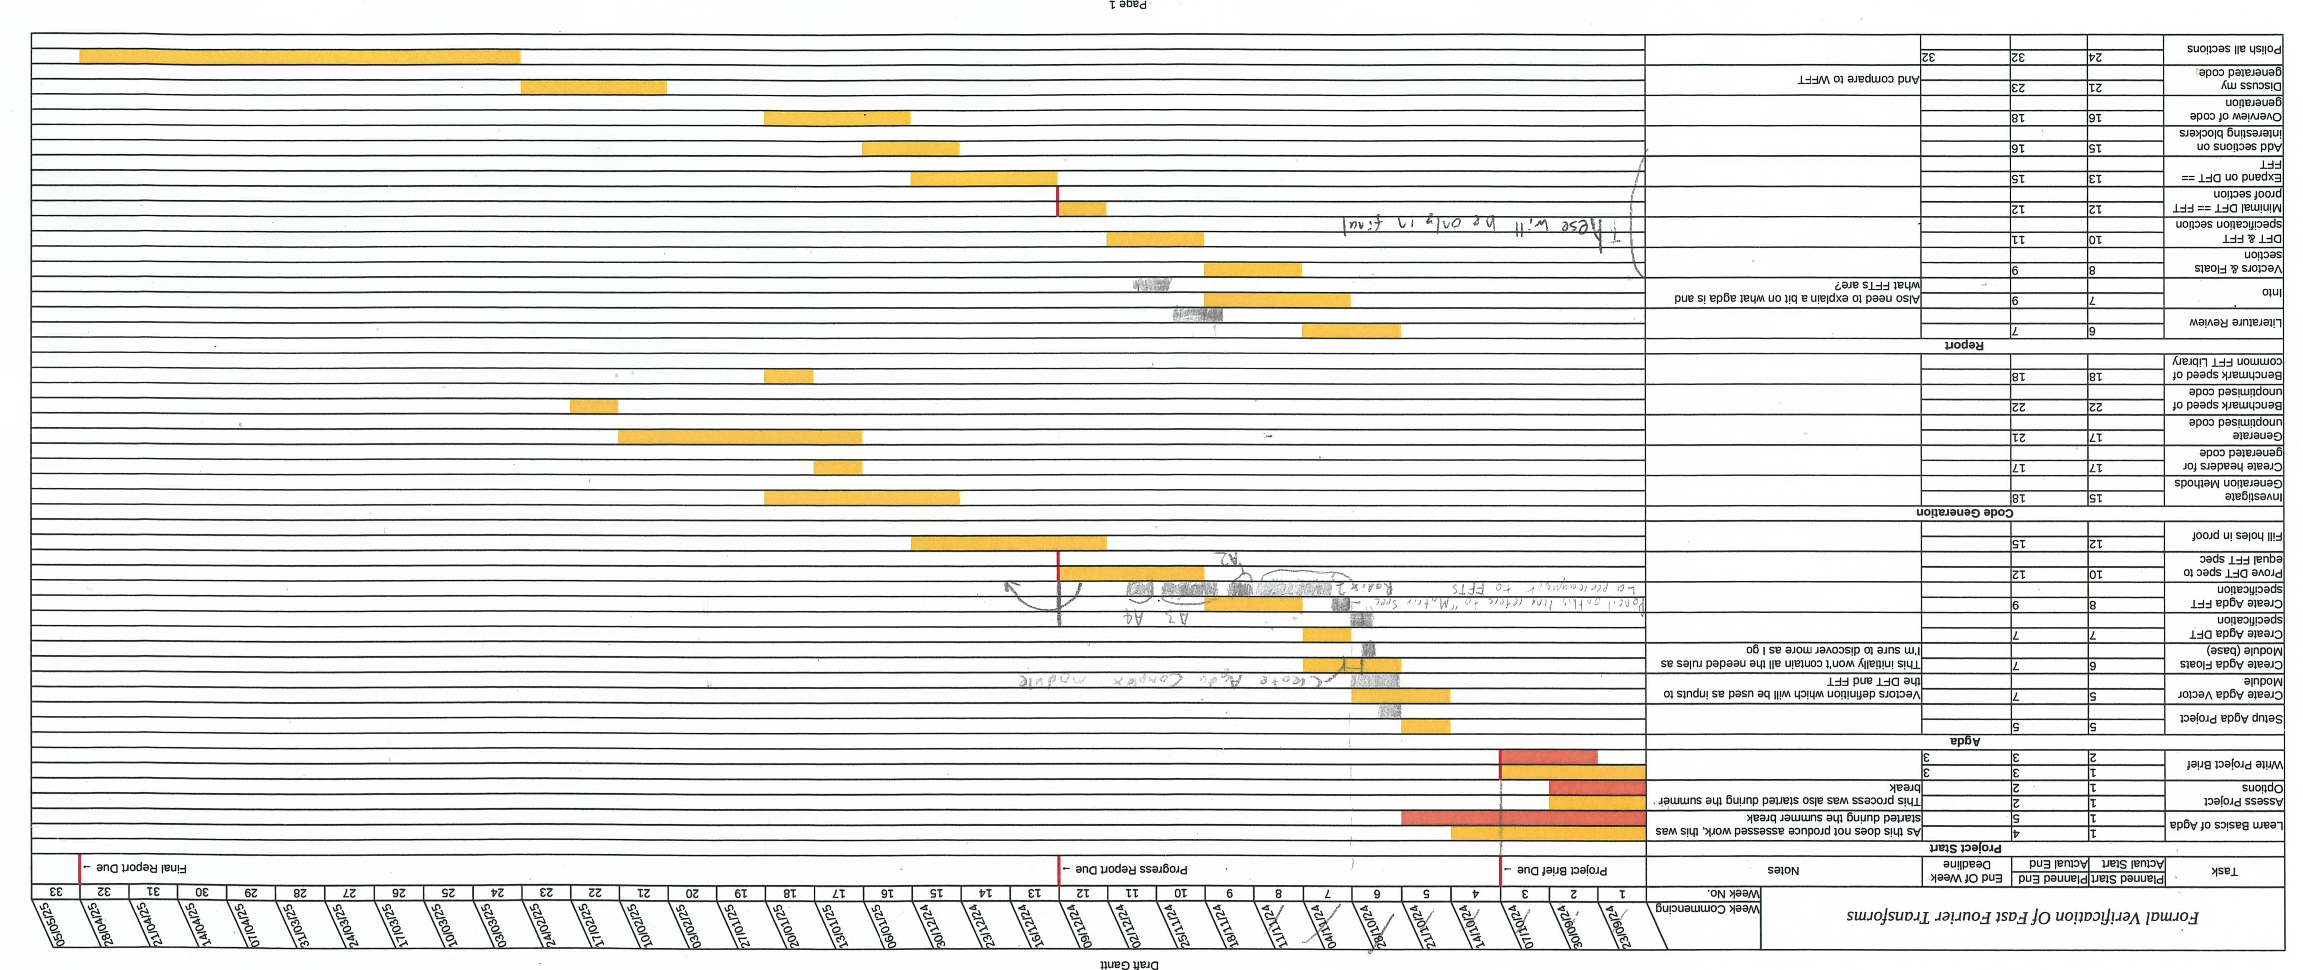
\includegraphics[angle=180, width=\linewidth]{Thesis/GanttHalfway.pdf}
        \caption{Gantt chart for the first half of the project}
        \label{fig:gantt_halfway}
    \end{figure}
\end{landscape}
\begin{landscape}
    \begin{figure}
        \centering
        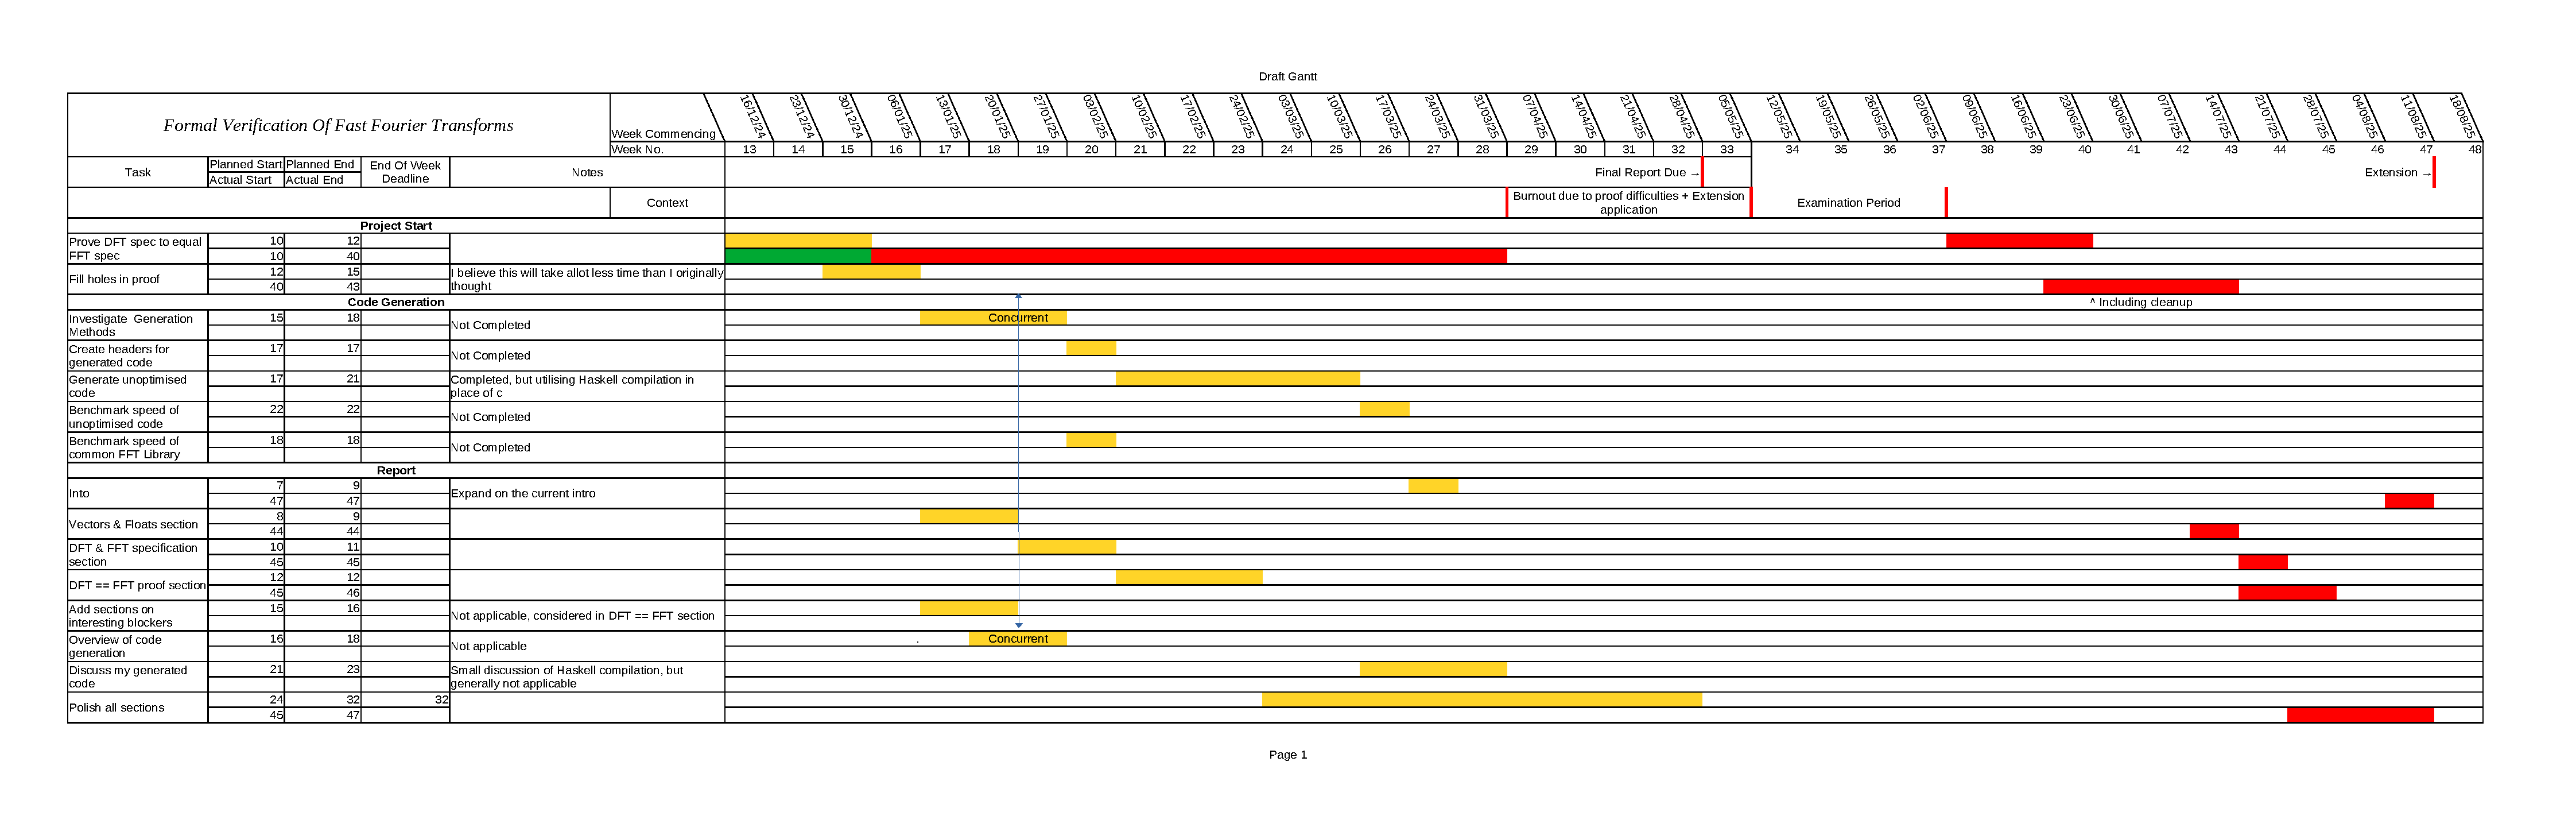
\includegraphics[width=\linewidth]{Thesis/GanttFinal.pdf}
        \caption{Final Gantt chart for the second half of the project}
        \label{fig:gantt_final}
    \end{figure}
\end{landscape}


\section{Conclusion}
This paper provides a formally verified implementation of the Cooley Tukey Fast 
Fourier Transform.
This implementation is built inductively, first defining representations of
tensors and complex numbers.
A trivial implementation of the Discrete Fourier Transform is then provided.
This is then used to define an implementation of the Fast Fourier Transform.

Unlike most verifiable implementations of the FFT, this implementations of the
FFT is radix generic and is defined on an abstract definition of Complex.
Defining the FFT generically allows for any non prime input
to be split optimally, and for the structure of any future parallelism to be 
defined at run time.

Given this general implementation of the FFT, I have then provided a proof that
it is equal to the DFT for all possible inputs.
With a basic implementation of the complex numbers, and a basic compiler,
this allowed for the generation of a runnable, verified, instance of the FFT.

In future research I wish to investigate the generation of optimised code, 
through translation into an intermediate language such as SaC.
The speed and floating point accuracy of such code would ideally be 
comparable to, or an improvement upon, the speed and accuracy of most similar
kernels in FFTW.
Should such comparison show significant improvement over the results of FFTW,
investigation into the generation of a kernel for FFTW would be possible.

Additionally, within the Agda community, this work allows future research 
projects to make use of the FFT interchangeably with the DFT.
This allows for future research into the verification of many signal processing 
algorithms, such as fast convolution or correlation, or for more general 
methods such as fast polynomial multiplication.


\clearpage
\bibliographystyle{IEEEtran}
\bibliography{Thesis/References}

\end{document}

